\documentclass[12pt,openany]{book}

%FIXME: for PRINT run for lulu or kdp, search for %PRINT

%\usepackage{pdf14}

\usepackage[shortlabels,inline]{enumitem}
\usepackage{ifpdf}
\usepackage[shortalphabetic,msc-links]{amsrefs}
\usepackage{mathtools}
\usepackage{amsmath}
\usepackage{amsfonts}
\usepackage{amssymb}
\usepackage{amsthm}
\usepackage{graphicx}
\usepackage{xcolor}
\usepackage{chngcntr}
\usepackage{titlesec}
\usepackage{import}
\usepackage{vogtwidebar}
\usepackage{nicefrac}
\usepackage{mathdots}
\usepackage{microtype}
\usepackage{cancel}
\usepackage{framed}
\usepackage{import}
\usepackage{varioref}
\usepackage{faktor}
\usepackage{tabto}

\usepackage{perpage}

\usepackage{tikz}
\usetikzlibrary{cd}
\usepackage{rotating}

\usepackage{cellspace}
\usepackage[toc,nopostdot,sort=use,nomain,automake]{glossaries}

%Palatino
\usepackage[theoremfont]{newpxtext}
\usepackage[vvarbb]{newpxmath}
\linespread{1.05}
\usepackage[scr=boondoxo]{mathalfa} % but we want the nice fancy script fonts

\usepackage[T1]{fontenc}

%symmetric for web
\usepackage[inner=1.2in,outer=1.2in,top=1in,bottom=1in]{geometry}
%PRINT asymetric for book
%\usepackage[inner=1.4in,outer=1.0in,top=1in,bottom=1in]{geometry}

\usepackage[margin=10pt,font=small,labelfont=bf,labelsep=colon,singlelinecheck=false]{caption}

%PRINT
% (not for the coil version or any version other than crown quatro using the
%  ghostscript conversion)
%Now cut page size a bit.  I'll run it through ghostcript anyway
%to convert to the right size, but this is good for crown quatro
%conversion, don't use for the full letter size versions
%\addtolength{\paperwidth}{-0.25in}
%\addtolength{\paperheight}{-0.5in}
%\addtolength{\topmargin}{-0.13in}
%\addtolength{\oddsidemargin}{-0.125in}
%\addtolength{\evensidemargin}{-0.125in}


\usepackage{url}
\usepackage{imakeidx}
\PassOptionsToPackage{hyphens}{url}
\usepackage{hyperref} % do NOT set [ocgcolorlinks] here!

%If you have an older tex installation you might need
%to comment out the next line:
%PRINT (COMMENT OUT FOR PRINT)
\usepackage[ocgcolorlinks]{ocgx2} %perhaps run without for lulu/kdp

\usepackage[all]{hypcap}

%\usepackage{draftwatermark}
%\SetWatermarkText{Work in progress!  Draft as of \today. May change substantially!}
%\SetWatermarkAngle{90}
%\SetWatermarkHorCenter{0.5in}
%\SetWatermarkColor[gray]{0.7}
%\SetWatermarkScale{0.16}
%\SetWatermarkScale{0.18}

\definecolor{gray75}{gray}{0.75}

\titleformat{\chapter}[hang]{\Huge\bfseries\filleft}%
{\thechapter$i$\hspace*{10pt}{\textcolor{gray75}{$\backslash\!\!\backslash$}}}%
{10pt}%
{}
[\vspace{-1ex}\rule{0.5\textwidth}{0.5pt}\rule{0.5\textwidth}{1pt}]

\titleformat{\section}[hang]{\Large\bfseries}%
{\thesection$i$\hspace*{10pt}{\textcolor{gray75}{$\backslash$}}}%
{10pt}%
{}%

\titleformat{\subsection}[hang]{\large\bfseries}%
{\thesubsection$i$\hspace*{10pt}{\textcolor{gray75}{$\cdot$}}}%
{10pt}%
{}%

\assignpagestyle{\chapter}{empty}


% Footnotes should use symbols, not numbers.  Numbered footnotes are
% evil, not using footmisc as it conflicts with hyperref
%\usepackage[perpage,symbol*]{footmisc}

\usepackage{footnote}

% The [2] would not use star
%\MakePerPage[2]{footnote}
\MakePerPage{footnote}
\renewcommand{\thefootnote}{\fnsymbol{footnote}}

% to avoid counter error on footnotes on first pass
\makeatletter
\gdef\@ctrerr{%
  \@latex@warning{Counter too large}}
\makeatother

% Enumitem extra penalties
\setlist[enumerate]{beginpenalty=100,midpenalty=-5}

% discourage pagebreak at end of display, put before \end{equation}
\newcommand{\avoidbreak}{\postdisplaypenalty=100}

\clubpenalty=500
\widowpenalty=500

%\overfullrule=10mm

% useful
\newcommand{\ignore}[1]{}

% analysis/geometry stuff
\newcommand{\ann}{\operatorname{ann}}
\renewcommand{\Re}{\operatorname{Re}}
\renewcommand{\Im}{\operatorname{Im}}
\newcommand{\Orb}{\operatorname{Orb}}
\newcommand{\hol}{\operatorname{hol}}
\newcommand{\aut}{\operatorname{aut}}
\newcommand{\Aut}{\operatorname{Aut}}
\newcommand{\codim}{\operatorname{codim}}
\newcommand{\sing}{\operatorname{sing}}
\newcommand{\ord}{\operatorname{ord}}
\newcommand{\dist}{\operatorname{dist}}
\newcommand{\Arg}{\operatorname{Arg}}
\newcommand{\Log}{\operatorname{Log}}

% reals
\newcommand{\esssup}{\operatorname{ess~sup}}
\newcommand{\essran}{\operatorname{essran}}
\newcommand{\innprod}[2]{\langle #1 | #2 \rangle}
\newcommand{\linnprod}[2]{\langle #1 , #2 \rangle}
\newcommand{\blinnprod}[2]{\bigl\langle #1 , #2 \bigr\rangle}
\newcommand{\supp}{\operatorname{supp}}
\newcommand{\Nul}{\operatorname{Nul}}
\newcommand{\Ran}{\operatorname{Ran}}
\newcommand{\sabs}[1]{\lvert {#1} \rvert}
\newcommand{\snorm}[1]{\lVert {#1} \rVert}
\newcommand{\babs}[1]{\bigl\lvert {#1} \bigr\rvert}
\newcommand{\bnorm}[1]{\bigl\lVert {#1} \bigr\rVert}
\newcommand{\Babs}[1]{\Bigl\lvert {#1} \Bigr\rvert}
\newcommand{\Bnorm}[1]{\Bigl\lVert {#1} \Bigr\rVert}
\newcommand{\bbabs}[1]{\biggl\lvert {#1} \biggr\rvert}
\newcommand{\bbnorm}[1]{\biggl\lVert {#1} \biggr\rVert}
\newcommand{\BBabs}[1]{\Biggl\lvert {#1} \Biggr\rvert}
\newcommand{\BBnorm}[1]{\Biggl\lVert {#1} \Biggr\rVert}
\newcommand{\abs}[1]{\left\lvert {#1} \right\rvert}
\newcommand{\norm}[1]{\left\lVert {#1} \right\rVert}

% sets (some)
\newcommand{\C}{{\mathbb{C}}}
\newcommand{\R}{{\mathbb{R}}}
\newcommand{\Z}{{\mathbb{Z}}}
\newcommand{\N}{{\mathbb{N}}}
\newcommand{\Q}{{\mathbb{Q}}}
\newcommand{\D}{{\mathbb{D}}}
\newcommand{\F}{{\mathbb{F}}}

% consistent
\newcommand{\bB}{{\mathbb{B}}}
\newcommand{\bC}{{\mathbb{C}}}
\newcommand{\bR}{{\mathbb{R}}}
\newcommand{\bZ}{{\mathbb{Z}}}
\newcommand{\bN}{{\mathbb{N}}}
\newcommand{\bQ}{{\mathbb{Q}}}
\newcommand{\bD}{{\mathbb{D}}}
\newcommand{\bF}{{\mathbb{F}}}
\newcommand{\bH}{{\mathbb{H}}}
\newcommand{\bO}{{\mathbb{O}}}
\newcommand{\bP}{{\mathbb{P}}}
\newcommand{\bK}{{\mathbb{K}}}
\newcommand{\bV}{{\mathbb{V}}}
\newcommand{\CP}{{\mathbb{CP}}}
\newcommand{\RP}{{\mathbb{RP}}}
\newcommand{\HP}{{\mathbb{HP}}}
\newcommand{\OP}{{\mathbb{OP}}}
\newcommand{\sA}{{\mathscr{A}}}
\newcommand{\sB}{{\mathscr{B}}}
\newcommand{\sC}{{\mathscr{C}}}
\newcommand{\sF}{{\mathscr{F}}}
\newcommand{\sG}{{\mathscr{G}}}
\newcommand{\sH}{{\mathscr{H}}}
\newcommand{\sM}{{\mathscr{M}}}
\newcommand{\sO}{{\mathscr{O}}}
\newcommand{\sP}{{\mathscr{P}}}
\newcommand{\sQ}{{\mathscr{Q}}}
\newcommand{\sR}{{\mathscr{R}}}
\newcommand{\sS}{{\mathscr{S}}}
\newcommand{\sI}{{\mathscr{I}}}
\newcommand{\sL}{{\mathscr{L}}}
\newcommand{\sK}{{\mathscr{K}}}
\newcommand{\sU}{{\mathscr{U}}}
\newcommand{\sV}{{\mathscr{V}}}
\newcommand{\sX}{{\mathscr{X}}}
\newcommand{\sY}{{\mathscr{Y}}}
\newcommand{\sZ}{{\mathscr{Z}}}
\newcommand{\fS}{{\mathfrak{S}}}

\newcommand{\interior}{\operatorname{int}}

% Topo stuff
\newcommand{\id}{\textit{id}}
\newcommand{\im}{\operatorname{im}}
\newcommand{\rank}{\operatorname{rank}}
\newcommand{\Tor}{\operatorname{Tor}}
\newcommand{\Torsion}{\operatorname{Torsion}}
\newcommand{\Ext}{\operatorname{Ext}}
\newcommand{\Hom}{\operatorname{Hom}}

%extra thingies
%\newcommand{\mapsfrom}{\ensuremath{\text{\reflectbox{$\mapsto$}}}}
\newcommand{\from}{\ensuremath{\leftarrow}}
\newcommand{\dhat}[1]{\hat{\hat{#1}}}

\definecolor{mypersianblue}{rgb}{0.11, 0.22, 0.73}

\hypersetup{
    pdfborderstyle={/S/U/W 0.5}, %this just in case ocg isn't there
    %PRINT (for print use the below and comment out the above):
    %pdfborder={0 0 0},
    citecolor=mypersianblue,
    filecolor=mypersianblue,
    linkcolor=mypersianblue,
    urlcolor=mypersianblue,
    pdftitle={Guide to Cultivating Complex Analysis},
    pdfsubject={Complex Analysis},
    pdfkeywords={one complex variable, complex analysis},
    pdfauthor={Jiri Lebl}
}

% Set up our index
\makeindex

% Very simple indexing
\newcommand{\myindex}[1]{#1\index{#1}}

% Quotes
\newcommand{\myquote}[1]{``#1''}

\author{Ji\v{r}\'i Lebl}

\title{Guide to Cultivating Complex Analysis}

% Don't include subsections
\setcounter{tocdepth}{1}

% Better "outline"
%\setcounter{tocdepth}{2}

\theoremstyle{plain}
\newtheorem{thm}{Theorem}[section]
\newtheorem{lemma}[thm]{Lemma}
\newtheorem{prop}[thm]{Proposition}
\newtheorem{cor}[thm]{Corollary}
\newtheorem{claim}[thm]{Claim}

\theoremstyle{remark}
\newtheorem{remark}[thm]{Remark}

\theoremstyle{definition}
\newtheorem{defn}[thm]{Definition}

\newtheoremstyle{exercise}% name
  {}% Space above
  {}% Space below
  {\itshape}% Body font
  {}% Indent amount 1
  {\bfseries \itshape}% Theorem head font
  {:}% Punctuation after theorem head
  {.5em}% Space after theorem head 2
  {}% Theorem head spec (can be left empty, meaning "normal")

% FIXME: Don't know if we should do this.  It is not as straightforward
%of a decision as it seems
% FIXME: It is also not finished in marking, chapter 1 till 1.4 is done
%\newcommand{\neededexmark}{$\blacklozenge$}
%\newcommand{\optneededexmark}{$\lozenge$}

\newenvironment{exbox}{%
    \def\FrameCommand{\vrule width 1pt \relax\hspace{10pt}}%
    \MakeFramed{\advance\hsize-\width\FrameRestore}%
}{%
    \endMakeFramed
}

\newenvironment{exparts}{%
    \leavevmode\begin{enumerate}[a),noitemsep,topsep=0pt,parsep=0pt,partopsep=0pt]
}{%
    \end{enumerate}
}
\newenvironment{exnumparts}{%
    \leavevmode\begin{enumerate}[1),noitemsep,topsep=0pt,parsep=0pt,partopsep=0pt]
}{%
    \end{enumerate}
}
\newenvironment{expartshor}[1]{%
    \begingroup%
    \NumTabs{#1}%
    \leavevmode%
    \par%
    \begin{enumerate*}[a),itemjoin={\tab}]
}{%
    \end{enumerate*}\endgroup\par
}

\newenvironment{myfig}{%
\begin{figure}[h!t]
\noindent\rule{\textwidth}{0.5pt}\vspace{12pt}\par\centering}%
{\par\noindent\rule{\textwidth}{0.5pt}
\end{figure}}

\newenvironment{myepigraph}{%
    \begin{quote}%
    \begingroup\itshape
}{%
    \endgroup%
    \end{quote}
}

\theoremstyle{exercise}
\newtheorem{exercise}{Exercise}[section]

\newtheoremstyle{example}% name
  {}% Space above
  {}% Space below
  {}% Body font
  {}% Indent amount 1
  {\bfseries}% Theorem head font
  {:}% Punctuation after theorem head
  {.5em}% Space after theorem head 2
  {}% Theorem head spec (can be left empty, meaning "normal")

\theoremstyle{example}
\newtheorem{example}[thm]{Example}

% referencing
\newcommand{\figureref}[1]{\hyperref[#1]{Figure~\ref*{#1}}}
\newcommand{\tableref}[1]{\hyperref[#1]{Table~\ref*{#1}}}
\newcommand{\chapterref}[1]{\hyperref[#1]{chapter~\ref*{#1}}}
\newcommand{\Chapterref}[1]{\hyperref[#1]{Chapter~\ref*{#1}}}
\newcommand{\Chdotref}[1]{\hyperref[#1]{Ch.~\ref*{#1}}}
\newcommand{\appendixref}[1]{\hyperref[#1]{appendix~\ref*{#1}}}
\newcommand{\Appendixref}[1]{\hyperref[#1]{Appendix~\ref*{#1}}}
\newcommand{\sectionref}[1]{\hyperref[#1]{section~\ref*{#1}}}
\newcommand{\subsectionref}[1]{\hyperref[#1]{\S~\ref*{#1}}}
\newcommand{\exerciseref}[1]{\hyperref[#1]{Exercise~\ref*{#1}}}
\newcommand{\exampleref}[1]{\hyperref[#1]{Example~\ref*{#1}}}
\newcommand{\thmref}[1]{\hyperref[#1]{Theorem~\ref*{#1}}}
\newcommand{\propref}[1]{\hyperref[#1]{Proposition~\ref*{#1}}}
\newcommand{\lemmaref}[1]{\hyperref[#1]{Lemma~\ref*{#1}}}
\newcommand{\corref}[1]{\hyperref[#1]{Corollary~\ref*{#1}}}
\newcommand{\defnref}[1]{\hyperref[#1]{Definition~\ref*{#1}}}
\newcommand{\remarkref}[1]{\hyperref[#1]{Remark~\ref*{#1}}}

% List of Symbols/Notation
\newglossary[nlg]{notation}{not}{ntn}{List of Notation}

\loadglsentries{notations}
\makeglossaries

\begin{document}

\ifpdf
  \pdfbookmark{Title Page}{title}
\fi
\newlength{\centeroffset}
\setlength{\centeroffset}{-0.5\oddsidemargin}
\addtolength{\centeroffset}{0.5\evensidemargin}
%\addtolength{\textwidth}{-\centeroffset}
\thispagestyle{empty}
\vspace*{\stretch{1}}
\noindent\hspace*{\centeroffset}\makebox[0pt][l]{\begin{minipage}{\textwidth}
\flushright
{\Huge\bfseries \sffamily Guide to Cultivating Complex Analysis}
\noindent\rule[-1ex]{\textwidth}{5pt}\\[2.5ex]
\hfill\emph{\Large \sffamily Working the Complex Field}
\end{minipage}}

\vspace{\stretch{1}}
\noindent\hspace*{\centeroffset}\makebox[0pt][l]{\begin{minipage}{\textwidth}
\flushright
{\bfseries 
%by
Ji{\v r}\'i Lebl\\[3ex]} 
\today
\\
(version 1.2)
\end{minipage}}

%\addtolength{\textwidth}{\centeroffset}
\vspace{\stretch{2}}


\pagebreak

\vspace*{\fill}

%\begin{small} 
\noindent
Typeset in \LaTeX.

\bigskip

\noindent
Copyright \copyright 2019--2021 Ji{\v r}\'i Lebl

%PRINT
% not for the coil version
%\noindent
%ISBN 979-8-6850-5792-1

%PRINT
% not for lulu
%\medskip
%\noindent
%Cover image: Field in South Czechia, \copyright 2008 Ji{\v r}\'i Lebl, all rights reserved.  Cover
%image cannot be reused in derivative works.


\bigskip

%\begin{floatingfigure}{1.4in}
%\vspace{-0.05in}
\noindent

\includegraphics[width=1.38in]{figures/license}
\quad

\includegraphics[width=1.38in]{figures/license2}
%\end{floatingfigure}

\bigskip

\noindent
\textbf{License:}
\\
This work is dual licensed under
the Creative Commons
Attribution-Non\-commercial-Share Alike 4.0 International License and
the Creative Commons
Attribution-Share Alike 4.0 International License.
To view a
copy of these licenses, visit
\url{https://creativecommons.org/licenses/by-nc-sa/4.0/}
or
\url{https://creativecommons.org/licenses/by-sa/4.0/}
or send a letter to
Creative Commons
PO Box 1866, Mountain View, CA 94042, USA\@.
%Creative Commons, 171 Second Street, Suite 300, San Francisco, California,
%94105, USA.

\bigskip

\noindent
You can use, print, duplicate, share this book as much as you want.  You can
base your own notes on it and reuse parts if you keep the license the
same.  You can assume the license is either the CC-BY-NC-SA or CC-BY-SA\@,
whichever is compatible with what you wish to do, your derivative works must
use at least one of the licenses.

\bigskip

\noindent
\textbf{Acknowledgments:}
\\
I would like to thank my students
Adam Cartisano,
Josiah Ireland,
Hoai Dao,
Haridas Das,
Uddhaba Pandey
for pointing out typos/errors
and helpful suggestions. 
%
%\bigskip
%
%\noindent
%During the writing of this book, 
%the author was in part supported by NSF grant DMS-1362337.

\bigskip

\noindent
\textbf{More information:}
\\
See \url{https://www.jirka.org/ca/} for more information
(including contacts).

\medskip

\noindent
The \LaTeX\ source for the book is available
for possible modification and customization
at github: \url{https://github.com/jirilebl/ca}


% For large print do this
%\large

\microtypesetup{protrusion=false}
\tableofcontents
\microtypesetup{protrusion=true}

%\addtocontents{toc}{\protect\vspace{-2\baselineskip}}
%\addtocontents{toc}{\protect\vspace{-\baselineskip}}
%\addtocontents{toc}{\protect\enlargethispage{\baselineskip}}

%%%%%%%%%%%%%%%%%%%%%%%%%%%%%%%%%%%%%%%%%%%%%%%%%%%%%%%%%%%%%%%%%%%%%%%%%%%%%%
%%%%%%%%%%%%%%%%%%%%%%%%%%%%%%%%%%%%%%%%%%%%%%%%%%%%%%%%%%%%%%%%%%%%%%%%%%%%%%
%%%%%%%%%%%%%%%%%%%%%%%%%%%%%%%%%%%%%%%%%%%%%%%%%%%%%%%%%%%%%%%%%%%%%%%%%%%%%%

\chapter*{Introduction} \label{ch:intro}
\addcontentsline{toc}{chapter}{Introduction}
\markboth{INTRODUCTION}{INTRODUCTION}

\begin{myepigraph}
If you cannot prove a man wrong, don't panic. You can always call him names.

---Oscar Wilde 
\end{myepigraph}

The purpose of this book is to teach a one-semester graduate course in
complex analysis for incoming graduate students.\footnote{I wrote it
specifically to teach Math 5283 at Oklahoma State University.}
The first seven chapters is a natural first semester in a two semester sequence where the second
semester could be several complex variables (e.g., \cite{scv:book})
or perhaps harmonic analysis.
It could perhaps be used for a more elementary two-semester sequence if the
appendix is covered first, and all the optional bits of the main text are
also covered.
We assume basic knowledge of undergraduate
analysis in the real variable, called advanced calculus in some schools.
The text assumes knowledge of metric spaces
and differential calculus in several variables, but if the reader is not
confident on these topics or has not yet seen them, the useful results
are presented (with proofs) in the appendices.
With that, a basic prerequisite for the
course would be at least a single semester of undergraduate analysis if the
appendices are also covered or read, and if the student has
seen metric spaces and mappings in $\R^2$, then the course
can just start in \Chapterref{ch:complexplane}.  Very basic undergraduate
linear and abstract algebra is also useful.

The analysis prerequisites can be mostly found in
\cites{ra:book,ra:book2,Rudin:principles}.  Further recommended
reading on complex analysis is \cites{Boas,Conway1,Conway2,Rudin,Ullrich}.
See the aptly named
\hyperref[ch:furtherreading]{Further Reading} chapter.

This book takes the view that we do not need to redefine and reprove
things that we have done in a basic undergraduate real analysis course,
especially with
regards to mappings of the plane.  We can quite quickly jump to
holomorphic functions as solutions of the Cauchy--Riemann equations,
for instance.
The connection is to understand both the derivative of 
a planar mapping and
multiplication by a complex number
as a $2 \times 2$ real matrix.
When we introduce line integrals, we connect
them to the line integrals the student has seen in calculus.
The inverse function theorem can be introduced early as
a consequence of the inverse function theorem in $\R^2$.
An outline of a pure complex analysis proof is left for later as an exercise.
These are not simply time saving measures.
The point is to stress that we are not defining some totally new and
different world.

We also try to introduce the $z,\bar{z}$ approach instead of just the
purely $x,y$ approach.  For example, we introduce and use the Wirtinger
operators.
It is really a better way to think about complex variables.

We try not to define any conflicting terminology or notation
with what the reader has learned before.
Mainly, the term \myquote{differentiable} is generally left for the real
derivative and we use \myquote{complex differentiable} when needed.  Although
to be sure, 
we generally write \myquote{(real) differentiable} or
\myquote{differentiable (in the real sense)} to
make it clear when we mean real differentiability.

Finally, some sections early in the book are marked with a $\star$ and those
can be easily skipped on first reading (though it does not mean they are not
important, just not necessary for what follows).  Skipping some may make it
possible to cover other later topics.

\medskip

The general dependence of the non-appendix chapters is the following diagram.
The way I ran my semester course was
to go through chapters
\ref{ch:complexplane}--\ref{ch:counting}, skipping the homotopy versions of
Cauchy, to get through basic theory of holomorphic functions,
then getting to \ref{ch:montelriemann} (Montel and Riemann mapping),
and some bits of \ref{ch:harmonic} (harmonic functions).
There are some extra topics for a different
plan such as
\ref{ch:weier} (Weierstrass factorization),
\ref{ch:runge} (Runge), and
\ref{ch:analcont} (analytic continuation).
\begin{equation*}
\begin{tikzcd}[cramped, row sep=small]
{\text{\Chdotref{ch:complexplane}}} \arrow[r] &
{\text{\Chdotref{ch:holanal}}} \arrow[r] &
{\text{\Chdotref{ch:cauchysimple}}} \arrow[r] &
{\text{\Chdotref{ch:log}}} \arrow[dl] \\
& & {\text{\Chdotref{ch:counting}}} \arrow[dl] \arrow[d]
\arrow[dr] \\
& {\text{\Chdotref{ch:montelriemann}}} \arrow[dl] \arrow[d] &
{\text{\Chdotref{ch:harmonic}}} &
{\text{\Chdotref{ch:weier}}}
\\
{\text{\Chdotref{ch:runge}}} &
{\text{\Chdotref{ch:analcont}}}
\\
\end{tikzcd}
\end{equation*}
The only reason why \ref{ch:runge} (Runge) depends on \ref{ch:montelriemann}
(Montel and Riemann mapping) is that we prove \lemmaref{lemma:patharoundK}
(around every compact there exists a cycle homologous to zero)
as an example application of Riemann mapping.

%%%%%%%%%%%%%%%%%%%%%%%%%%%%%%%%%%%%%%%%%%%%%%%%%%%%%%%%%%%%%%%%%%%%%%%%%%%%%%
%%%%%%%%%%%%%%%%%%%%%%%%%%%%%%%%%%%%%%%%%%%%%%%%%%%%%%%%%%%%%%%%%%%%%%%%%%%%%%
%%%%%%%%%%%%%%%%%%%%%%%%%%%%%%%%%%%%%%%%%%%%%%%%%%%%%%%%%%%%%%%%%%%%%%%%%%%%%%

\chapter{The Complex Plane} \label{ch:complexplane}

\begin{myepigraph}
It's clearly a budget. It's got a lot of numbers in it.

---George W.\ Bush
\end{myepigraph}

%%%%%%%%%%%%%%%%%%%%%%%%%%%%%%%%%%%%%%%%%%%%%%%%%%%%%%%%%%%%%%%%%%%%%%%%%%%%%%

\section{Complex numbers} \label{sec:complexnums}

Modern\footnote{In this context, \emph{modern}
means \myquote{later than the middle ages.}}
mathematics
is taking a false statement such as
\myquote{all polynomials have a root} and redefining what a
\myquote{root} could be, that is,
redefining \myquote{number,}
so that the statement is true.
In this instance, we arrive at the complex numbers.
Although this technique (moving the goalposts)
feels like cheating, it gave us
essentially all the mathematics we know, both pure and applied.
This same
technique starts with the natural numbers
\glsadd{not:N}$\N = \{ 1,2,3,\ldots \}$, the only
numbers obvious from nature,
and gives us zero and negative numbers producing the integers
\glsadd{not:Z}$\Z$, so that we can solve equations such as $n+2 = 1$.
From \glsadd{not:Z}$\Z$, we define the rational numbers
\glsadd{not:Z}$\Q$ to solve\footnote{%
Do we really solve $2x=1$ by writing $x = \nicefrac{1}{2}$?  After all, 
$\nicefrac{1}{2}$ is just a placeholder for an object that we can't describe
in a way other than
\myquote{whatever $1$ divided by $2$ would be if it existed.}}
equations such as $2x=1$.  We extend
\glsadd{not:Q}$\Q$ to the real numbers \glsadd{not:R}$\R$
to solve equations such as $x^2=2$.  Actually our definition 
of the real numbers is such that we get theorems like the
intermediate value theorem, Bolzano--Weierstrass,
etc.  It is then not much of a stretch to do the same thing when trying
to solve $z^2+1=0$.  Just as with the real numbers,
the consequences of adding $\sqrt{-1}$ to the mix are much more
profound than just finding roots of polynomials.

Interestingly, while the step into analysis with the real numbers
is a step into the abyss, the step into analysis with the complex numbers is a
step into a fairytale wonderland.  A first-year real analysis course
crushes the student's hopes and dreams.  Most reasonable statements
are false and bizarre counterexamples abound.
On the other hand, a complex analysis course fills the student with
unrealistic optimism.  It is replete with na\"ive and silly statements
that only a bad calculus student could entertain.\footnote{%
E.g.:  If you can differentiate once, you can differentiate twice.
Every function acts sort of like a linear function.
If all derivatives are zero at a point, the function is constant.
Etc.}
The two are the good-cop bad-cop, the yin-yang,
of contemporary analysis.

\subsection{The complex numbers as the plane}

You have surely seen the complex number field,
but let us review its definition anyway.
As a set, let the \emph{\myindex{complex number field}}
\glsadd{not:C}$\C$ be the set $\R^2 = \R \times \R$.
The set is a plane, so we call it the \emph{\myindex{complex plane}}%
\footnote{Although there is that odd mathematician out there that
thinks that the \emph{complex plane} is $\C^2 = \C \times \C$.
If you hear someone say that, politely whack them over the head for me.}.
To make it a field, we define addition and product:
\begin{align*}
(a,b) + (c,d) & \overset{\text{def}}{=} (a+b,c+d) , \\
(a,b) (c,d) & \overset{\text{def}}{=} (ac-bd,bc+da) .
\end{align*}

\begin{exbox}
\begin{exercise}%[\neededexmark]
Check that $\C$ is a field, where the additive
identity is $0=(0,0)$ and the multiplicative identity is $1=(1,0)$.
That is, $\C$ is an abelian group under addition,
the nonzero complex numbers are an abelian group under multiplication,
and the distributive law holds.  Hint: The multiplicative inverse of $(a,b)$
is $\left(\frac{a}{a^2+b^2},\frac{-b}{a^2+b^2}\right)$.
\end{exercise}
\end{exbox}

When we write a real number $x$, we identify it with the
complex number $(x,0)$.
With this identification $\R \subset \C$.
We also define the \emph{\myindex{imaginary unit}}%
\footnote{Beware of engineers; they think it is called $j$, despite there
being no \myquote{j} in \myquote{imaginary.}}%
\glsadd{not:i}
\begin{equation*}
i \overset{\text{def}}{=} (0,1) .
\end{equation*}
With this notation, $(x,y) = x+iy$.  From now on, $x+iy$ is the only way we
will write
the complex numbers in terms of the coordinates $x$ and $y$.
We call $x+iy$ the \emph{\myindex{cartesian}}
form of the complex number.
The number $i$ has the magical property that
\begin{equation*}
i^2 = -1 .
\end{equation*}
For this reason we sometimes%
\footnote{There are those that \emph{always} write $\sqrt{-1}$ instead of $i$.
Those people also deserve a good whack.}
write $i = \sqrt{-1}$.
Note that there is another square root of $-1$, that is, $-i$.
The numbers $i$ and $-i$ are the solutions to $z^2+1=0$.
We will prove later that every polynomial has roots over the complex numbers.

Given a complex number $z=x+iy$, its \myquote{evil twin} is 
the \emph{\myindex{complex conjugate}} of $z$:
\glsadd{not:conj}%
\begin{equation*}
\bar{z} \overset{\text{def}}{=} x-iy.
\end{equation*}
The number $x$ is called the
\emph{\myindex{real part}} and $y$ is called the
\emph{\myindex{imaginary part}}.  We write
\glsadd{not:real}%
\glsadd{not:imag}%
\begin{equation*}
\Re z = 
\Re (x+iy) =
\frac{z+\bar{z}}{2}
= x, \qquad 
\Im z = 
\Im (x+iy) =
\frac{z-\bar{z}}{2i}
=
y .
\end{equation*}
A particularly useful observation is that we wrote the
real part and the imaginary part in terms of $z$ and $\bar{z}$.
Any expression we write in terms of the real and imaginary parts of $z$,
 we can equally well write in terms of $z$ and $\bar{z}$.  And vice versa.
For example,
\begin{equation*}
x^3 + y^3 + 3ixy
=
{\left( \frac{z+ \bar{z}}{2} \right)}^3 + 
{\left( \frac{z- \bar{z}}{2i} \right)}^3 + 
3i {\left( \frac{z+ \bar{z}}{2} \right)} 
{\left( \frac{z- \bar{z}}{2i} \right)} ,
\end{equation*}
or
\begin{equation*}
z^2 - i \bar{z}^2 + z \bar{z}
=
{(x+iy)}^2 - i {(x-iy)}^2 + 
(x+iy)(x-iy) .
\end{equation*}
It may seem that an expression in terms of $z$ and $\bar{z}$ is more
complicated.  Namely, $z$ and $\bar{z}$ are not
\myquote{independent variables.}  However, it is particularly powerful to
think in terms of $z$ and $\bar{z}$ instead of $x$ and $y$, and to pretend
in many contexts as if $z$ and $\bar{z}$ were actually independent
variables.

\subsection{The geometry and topology of the plane}

The size of $z$ is measured by the so-called \emph{\myindex{modulus}},
which is just the \emph{\myindex{euclidean distance}}
of $0$ and $z$:
\glsadd{not:mod}%
\begin{equation*}
\sabs{z} \overset{\text{def}}{=} \sqrt{z \bar{z}} = \sqrt{x^2+y^2} .
\end{equation*}
More simply, ${\sabs{z}}^2 = z\bar{z}$.
Notice $\sabs{z} \geq 0$, and $\sabs{z} = 0$
if and only if $z=0$.

\begin{prop}[Cauchy--Schwarz and the triangle inequality]
If $z,w \in \C$, then
\begin{enumerate}[(i)]
\item
$\sabs{\Re z\bar{w}} \leq \sabs{z} \sabs{w}$ \quad (Cauchy--Schwarz inequality\footnote{%
Some say it should be Cauchy--Bunyakovsky--Schwarz, but that is wrong.
Bunyakovsky and Schwarz proved the infinite-dimensional version.  This is
just Cauchy inequality, but lamentably that name refers to a different
inequality, one that we will call the Cauchy estimates.}, note: $\Re z
\bar{w}$ is the real dot product),\index{Cauchy--Schwarz}
\item
$\sabs{z+w} \leq \sabs{z} + \sabs{w}$ \quad (Triangle inequality).%
\index{triangle inequality!complex numbers}
\end{enumerate}
\end{prop}

\begin{proof}
The modulus squared of a complex number is always nonnegative.
Thus,
\begin{equation*}
\begin{split}
0 & \leq {\sabs{z\bar{w}-\bar{z}w}}^2 \\
  & =    (z\bar{w}-\bar{z}w)(\bar{z}w-z\bar{w}) \\
  & =    2z\bar{z}w\bar{w} - z^2\bar{w}^2 - \bar{z}^2w^2 \\
  & =    4z\bar{z}w\bar{w} - {(z\bar{w}+\bar{z}w)}^2 \\
  & =    {\bigl(2\sabs{z}\sabs{w}\bigr)}^2 - {\bigl(2 \Re z\bar{w}\bigr)}^2 .
\end{split}
\end{equation*}
This proves Cauchy--Schwarz.  We prove the triangle inequality
via Cauchy--Schwarz:
\begin{equation*}
\begin{split}
{\sabs{z+w}}^2 & =    (z+w)(\bar{z}+\bar{w}) \\
               & =    z\bar{z} + w\bar{w} + z\bar{w} + \bar{z}w \\
               & \leq z\bar{z} + w\bar{w} + 2 \sabs{z}\sabs{w} \\
               & =    {\bigl(\sabs{z}+\sabs{w}\bigr)}^2 . \qedhere
\end{split}
\end{equation*}
\end{proof}

\begin{exbox}
\begin{exercise}
Prove the \emph{\myindex{polarization identity}}
$4 z\bar{w} =
{\sabs{z+w}}^2-{\sabs{z-w}}^2 +i \bigl( {\sabs{z+iw}}^2 - {\sabs{z-iw}}^2 \bigr)$.
\end{exercise}
\end{exbox}

The distance between two numbers $z$ and $w$ is measured by
\begin{equation*}
\sabs{z-w} .
\end{equation*}
This distance makes $\C$ into a complete metric space.  By complete, we mean that
Cauchy sequences have limits.  See \Appendixref{ap:metric}
for an introduction to metric spaces.

\begin{prop}
Complex addition, multiplication, division, and conjugation are continuous:
Suppose $\{ a_n \}$ and $\{ b_n \}$ are two convergent sequences
of complex numbers.  Then,
\begin{enumerate}[(i)]
\item
$\lim\limits_{n\to\infty} (a_n + b_n) = 
\left(\lim\limits_{n\to\infty} a_n \right) +
\left(\lim\limits_{n\to\infty} b_n \right)$,
\item
$\lim\limits_{n\to\infty} a_n b_n = 
\left(\lim\limits_{n\to\infty} a_n \right)
\left(\lim\limits_{n\to\infty} b_n \right)$,
\item
$\lim\limits_{n\to\infty} \frac{1}{a_n} = \frac{1}{\lim\limits_{n\to\infty} a_n}$,
as long as $\lim\limits_{n\to\infty} a_n \not= 0$,
\item
$\lim\limits_{n\to\infty} \bar{a}_n = 
\overline{\lim\limits_{n\to\infty} a_n}$.
\end{enumerate}
\end{prop}

\begin{exbox}
\begin{exercise}%[\neededexmark]
Prove the proposition.
\end{exercise}
\end{exbox}

The basic neighborhood (that is, an
open ball) in $\C$
is called a \emph{\myindex{disc}}.
Given $p \in \C$ and $r > 0$, define the disc of radius $r$ around
$p$
as
\glsadd{not:disc}%
\begin{equation*}
\Delta_r(p)
\overset{\text{def}}{=}
\bigl\{ z \in \C : \sabs{z-p} < r \bigr\} .
\end{equation*}
A disc centered at the origin of radius $1$ is called the
\emph{\myindex{unit disc}}
\glsadd{not:D}%
\begin{equation*}
\D
\overset{\text{def}}{=}
\Delta_1(0)
=
\bigl\{ z \in \C : \sabs{z} < 1 \bigr\} .
\end{equation*}
The unit disc will come up often in this course, as it turns out that
a lot of complex analysis can be done by looking at just the unit disc.

A useful \myquote{version} of the unit disc, is the \emph{\myindex{upper half-plane}}:
\glsadd{not:H}%
\begin{equation*}
\bH 
\overset{\text{def}}{=}
\bigl\{
z \in \C : \Im z > 0
\bigr\} .
\end{equation*}
We will see in a moment that $\D$ and $\bH$ are equivalent in a
very nice way.
Things done on the unit disc can just as well be done on the upper half-plane.

The following definition is perhaps somewhat unnecessary, but it is 
easier to write and say than \emph{open and connected}, and it is commonly
used in complex analysis.\footnote{We generally consider our sets
also nonempty, but usually the statements of results for empty open sets or
domains are simply vacuous.}

\begin{defn}
An open and connected set $U \subset \C$ is called a
\emph{\myindex{domain}}.\footnote{Perhaps \myquote{domain} is a tad unfortunate since
we also call the $X$ in $f \colon X \to Y$ a \myquote{domain} of the function,
even if $X$ is not a domain in the sense of topology.}
\end{defn}

\subsection{Complex-valued functions}

It is possible that the analysis you have seen so far in your mathematical
career has been for real-valued functions $f \colon X \to \R$.  In this
book, we are concerned with complex-valued functions $f \colon X \to \C$.
The results for real-valued functions are then applied by thinking of
either the components of $f$ separately or by thinking of $\C$ as the
real vector space $\R^2$.

When we find ourselves in the possession of a complex-valued function
$f \colon X \to \C$ we write $u = \Re f$
and $v = \Im f$ for real-valued functions $u,v \colon X \to \R$, and then
\begin{equation*}
f = u+iv .
\end{equation*}

If $X \subset \C$, then we think of $X \subset \R^2$.
A derivative in $x$ or $y$ (where $z=x+iy$) is then applied to the
components (just as if $f$ was valued in $\R^2$):
\begin{equation*}
\frac{\partial f}{\partial x} = 
\frac{\partial u}{\partial x} + i
\frac{\partial v}{\partial x}
\qquad\text{and}\qquad
\frac{\partial f}{\partial y} = 
\frac{\partial u}{\partial y} + i
\frac{\partial v}{\partial y} .
\end{equation*}

If $X \subset \R$, that is, if $f$ is a complex-valued
function of one real variable, then $f' = u' + iv'$.
Equivalently, we treat $f$ as a function from $\R$ to $\R^2$
and hence $f'$ is a $2 \times 1$ matrix---a column vector, or in other words
$f'$ represents a complex number if we are identifying $\C$ and $\R^2$.

Similarly when integrating.  For $f \colon [a,b] \to \C$,
we say $f$ is (Riemann) integrable if $u$ and $v$ are, and then
\begin{equation*}
\int_a^b f(t) \, dt = 
\int_a^b u(t) \, dt + i \int_a^b v(t) \, dt .
\end{equation*}
Indeed, that is the way one integrates vector-valued functions
for any vector space, and $\C = \R^2$ is a vector space.
Basic analysis tells us that
if given a Riemann integrable
real-valued function $u \colon [a,b] \to \R$,
then $\abs{u}$ is Riemann
integrable and $\abs{\int_a^b u(t) \, dt} \leq \int_a^b \sabs{u(t)} \, dt$.
Similar result holds for complex-valued functions.

\begin{prop} \label{prop:inttriangleineq}
Suppose $f \colon [a,b] \to \C$ is (Riemann) integrable.  Then $\sabs{f}$ is
(Riemann) integrable and
\begin{equation*}
\abs{\int_a^b f(t) \, dt} \leq 
\int_a^b \abs{f(t)} \, dt .
\end{equation*}
\end{prop}

\begin{exbox}
\begin{exercise}%[\neededexmark]
Prove the proposition.  Hint: After you know integrability, consider
a Riemann sum and the regular triangle inequality.
\end{exercise}
\end{exbox}

\subsection{Matrix representation of complex numbers}

As $\C$ is $\R^2$, we can think of
$\C$ as a real two-dimensional vector space by forgetting about the
complex multiplication.  The standard basis is $1$ and $i$.
To put multiplication back into the picture, we think of linear operators
on $\R^2$.
Given a complex number $\xi$, the map $z \mapsto  \xi z$ is a
real-linear operator\footnote{$L \colon \C \to \C$ is real-linear if
$L(a z + b w) = aL(z)+bL(z)$ for all $a,b \in \R$ and $z,w \in \C$.}.
A real-linear operator on $\R^2$ is given by a $2 \times 2$ real
matrix.
Namely, the complex number $a+ib$ can be represented by the $2 \times 2$ matrix
\begin{equation} \label{eq:complexnumbermatrix}
\begin{bmatrix}
a & -b \\
b & a
\end{bmatrix} .
\end{equation}
Let us check.
If we think of a complex number $a+ib$ as a matrix
and $c+id$ as a column vector,
then complex multiplication makes sense as matrices:
\begin{equation*}
\begin{bmatrix}
a & -b \\
b & a
\end{bmatrix}
\begin{bmatrix}
c \\
d 
\end{bmatrix}
=
\begin{bmatrix}
ac-bd \\
bc+ad
\end{bmatrix} .
\end{equation*}
The matrices
\begin{equation*}
1 \quad ``{}={}'' \quad
\begin{bmatrix}
1 & 0 \\
0 & 1
\end{bmatrix} \qquad \text{and} \qquad
i \quad ``{}={}'' \quad
\begin{bmatrix}
0 & -1 \\
1 & 0
\end{bmatrix} 
\end{equation*}
are the identity and the rotation counterclockwise by $90$ degrees
respectively.  Precisely what we expect multiplication by $1$ and $i$
to do.

Complex conjugation is also real-linear
operator and can be represented by the matrix $\left[ \begin{smallmatrix} 1 & 0 \\ 0 &
-1 \end{smallmatrix} \right]$.  Notice that complex conjugation is
not a multiplication by a complex number.
Below you will prove, however,
that multiplications by complex numbers together with conjugation do 
in fact \myquote{generate} all the real-linear operators.

For those matrices representing complex numbers,
we can also multiply the $2 \times 2$ matrices themselves,
and this matrix multiplication is the same as multiplication of the complex
numbers.  Similarly with addition.
That is, we can view the field of complex numbers as a subring of $M_2(\R)$
(exercise below).

\begin{exbox}
\begin{exercise}
Prove that a) the matrix multiplication on matrices of the form
\eqref{eq:complexnumbermatrix}
is commutative and b) reproduces the complex
number multiplication, and that these matrices form a subring of $M_2(\R)$.
c) Prove that nonzero matrices of this form are
invertible (the subring is a field).  Specifically, notice the
determinant appearing in the denominator for the multiplicative inverse.
\end{exercise}

\begin{exercise}
Prove that if the $2 \times 2$ matrix $M$ represents a complex number
$a+ib$, then $M$ has two eigenvalues: $a \pm i b$ with the corresponding
eigenvectors $\left[ \begin{smallmatrix} 1 \\ \mp i \end{smallmatrix}
\right]$.
\end{exercise}

\begin{exercise} \label{exercise:reallinmap}
Prove that every real-linear operator on $\C$ (that is, every 
$2 \times 2$ real matrix $M$) can be represented 
by two complex numbers $\xi$ and $\zeta$, and the formula
$z \mapsto \xi z + \zeta \bar{z}$.
\end{exercise}

\begin{exercise}
\begin{exparts}
\item
Suppose a $2 \times 2$ real matrix $M$ represents multiplication by $\xi \in \C$.
Show that $\det M = \sabs{\xi}^2$.
\item
Suppose a $2 \times 2$ real matrix $M$ is represented by $z \mapsto \xi z + \zeta
\bar{z}$ (see previous exercise).
Show that $\det M = \sabs{\xi}^2 - \sabs{\zeta}^2$.
\end{exparts}
\end{exercise}
\end{exbox}

This representation of complex numbers comes up quite often in applications.
For instance, 
an $m \times n$ complex matrix can be represented by a
$2m \times 2n$ real matrix by replacing each entry by a $2 \times 2$ matrix.
So software set up for working with real matrices can easily be duped into
working with complex matrices.

For us, the main application will be to understand the derivative of a
complex-valued function of a complex variable $f \colon \C \to \C$.
Thinking of the function as a mapping $f \colon \R^2 \to \R^2$,
the real derivative of $f$ is a $2 \times 2$ matrix.  The
object of study of complex analysis, the holomorphic (or analytic)
functions, are those functions whose real derivative matrix corresponds to a
multiplication by a complex number.

%%%%%%%%%%%%%%%%%%%%%%%%%%%%%%%%%%%%%%%%%%%%%%%%%%%%%%%%%%%%%%%%%%%%%%%%%%%%%%

\section{Polar form and the exponential}

\subsection{The exponential} \label{subsection:firstdefexp}

The exponential is the most fundamental and useful function in complex
analysis.  Assume we know $e^x$ for real numbers.  Define $e^z$
for complex numbers (see
\figureref{fig:complexexpgraphs}):
\glsadd{not:exp}%
\begin{equation*}
\exp(z) =
e^{z} = 
e^{x+iy}
\overset{\text{def}}{=}
e^x e^{iy}
=
e^x\cos y + i e^x \sin y .
\end{equation*}
\begin{myfig}
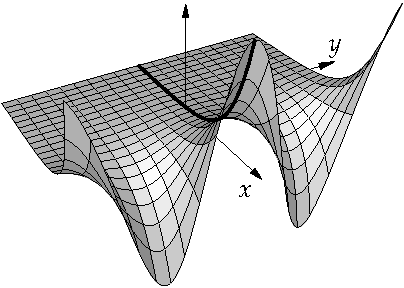
\includegraphics{figures/realexp}
\qquad
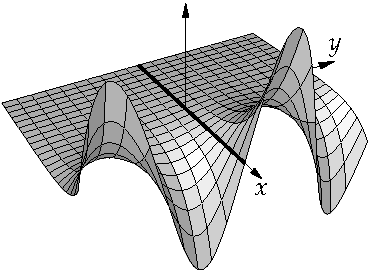
\includegraphics{figures/imagexp}
\caption{Graphs of the real part (left) and imaginary part (right)
of the complex exponential $e^z = e^{x+iy}$.
The plot of the real exponential ($y=0$)
is marked in a bold line.\label{fig:complexexpgraphs}}
\end{myfig}

The definition agrees with the standard exponential for real numbers (when
$y=0$).  Furthermore,
\begin{equation*}
e^{\bar{z}} = 
e^{x-iy} =
e^x\cos y - i e^x \sin y  = \overline{e^{z}} ,
\end{equation*}
and
\begin{equation*}
\sabs{e^{z}} = 
\sabs{e^{x-iy}} =
e^x .
\end{equation*}
It is possible to define the complex exponential without resorting to
the real exponential, sine, and cosine, and we will do so in due course.
But we are impatient and we want something to play around with now, without waiting.

\begin{prop}
For any two complex numbers $z,w \in \C$,
\begin{equation*}
e^{z+w} = e^z e^w .
\end{equation*}
\end{prop}

\begin{exbox}
\begin{exercise}%[\neededexmark]
Prove the proposition using the definition and trigonometric identities.
\end{exercise}
\end{exbox}

We remark that $e^z$ is the unique continuous
function on $\C$ that satisfies $e^{z+w} = e^z e^w$ and $e^0 = 1$.
Let us not worry about proving that.
For real $\theta$, the definition
of the exponential gives the so-called
\emph{\myindex{Euler's formula}}:
\begin{equation*}
e^{i\theta}
=
\cos \theta + i \sin \theta .
\end{equation*}
The formula says that for real $\theta$,
\begin{equation*}
\cos \theta = \Re e^{i\theta} = \frac{e^{i\theta}+e^{-i\theta}}{2} ,
\qquad
\sin \theta = \Im e^{i\theta} = \frac{e^{i\theta}-e^{-i\theta}}{2i} .
\end{equation*}
We define cosine and sine for complex numbers by plugging
those numbers
into the formulas above, now that we know how to evaluate the exponential:
\begin{equation*}
\cos z \overset{\text{def}}{=} \frac{e^{iz}+e^{-iz}}{2} ,
\qquad
\sin z \overset{\text{def}}{=} \frac{e^{iz}-e^{-iz}}{2i} .
\end{equation*}

\subsection{Polar coordinates}

As complex numbers are just the plane, we can use polar coordinates
to represent complex numbers.
That is, $x = r \cos \theta$ and $y= r \sin \theta$.
We write this form as
\begin{equation*}
z = x+iy = r e^{i \theta} .
\end{equation*}
Here, $r = \sabs{z} = \sqrt{x^2+y^2}$ is the modulus, and 
$\theta$ is the angle that $x+iy$ makes with the real axis (the $x$-axis).
The $\theta$ is called the \emph{\myindex{argument}}.  See
\figureref{fig:polarcoords}.
The reason for the notation is the
Euler's formula, so
\begin{equation*}
z = r e^{i\theta} = r\cos \theta + i r\sin \theta  = x+iy .
\end{equation*}

\begin{myfig}
\subimport*{figures/}{polarcoords.pdf_t}
\caption{Polar coordinates.\label{fig:polarcoords}}
\end{myfig}

Polar form is particularly nice for multiplication and for powers.
Suppose $z = r e^{i\theta}$ and $w = s e^{i \psi}$, then
\begin{equation*}
zw =
r e^{i \theta} s e^{i \psi} = 
rs e^{i (\theta+ \psi)},
\qquad
\frac{1}{z} =
\frac{1}{r e^{i \theta}} =
\frac{1}{r} e^{-i \theta} ,
\qquad
z^n =
{\bigl(r e^{i \theta}\bigr)}^n =
r^n e^{i n\theta} .
\end{equation*}
Multiplication rotates by the argument and scales by the modulus.
Namely, we see again that multiplication by $i = e^{i \pi / 2}$ is
rotation counterclockwise by $90$ degrees.
The downside is that the polar form is particularly terrible for addition.
You win some, you lose some.

\begin{exbox}
\begin{exercise}
Let $z,w$ be two nonzero complex numbers and let
$\ell_z$ and $\ell_w$ be the lines through the origin and
$z$ and $w$ respectively.  Write $\theta$ for the angle between $\ell_z$ and
$\ell_w$.  Then prove that
$\Re z\bar{w} = \sabs{z} \sabs{w} \cos \theta$.
Note that $\Re z\bar{w}$ is the standard real dot product in $\R^2$, and so
this is the formula for the dot product from calculus.
\end{exercise}
\end{exbox}

\subsection{The argument}

We attempt to define the argument of $z = re^{i\theta}$ as
\glsadd{not:arg}%
\begin{equation*}
\arg z
\overset{\text{def?}}{=}
\theta ,
\end{equation*}
but we run up against the problem that if $\theta$ is an argument of $z$,
then so is $\theta+2\pi$, $\theta-2\pi$, or $\theta + k 2\pi$ for any
integer $k$.  In other words,
$\arg z$ is not a function in the classical sense, but a
\emph{\myindex{multivalued function}}%
\footnote{Non-complex analysts will sometimes claim that a multivalued
function is nonsense, but you can safely ignore those troublemakers.}.  The correct
definition is
\glsadd{not:arg}%
\begin{equation*}
\arg z
\overset{\text{def}}{=}
\ldots,\theta - 4\pi,
\theta - 2\pi,
\theta ,
\theta + 2\pi,
\theta + 4\pi, \ldots
\end{equation*}
One more minor issue remains.  If $z=0$, then $z=0=0 e^{i\theta}$ for any
$\theta$ whatsoever.  Therefore, we only define the argument for nonzero
$z$.

It may at times be useful to nail down a particular number for the argument.
We define the \emph{\myindex{principal branch of $\arg$}} as
\glsadd{not:Arg}%
\begin{equation*}
\Arg z
\overset{\text{def}}{=}
\theta, \qquad \text{where } -\pi < \theta \leq \pi.
\end{equation*}
It may seem like a good solution to the multivaluedness of $\arg$, but
one's hopes are dashed by the cruel reality of $\Arg$ not being continuous
on the negative real axis.  See \figureref{fig:arggraph}.
The principal branch is somewhat less useful than one may think.
There is also the issue that not everyone agrees
on what \myquote{principal branch} means; some mathematicians sacrifice the
positive real axis and let $\theta$ be in the range $[0,2\pi)$.

\begin{myfig}
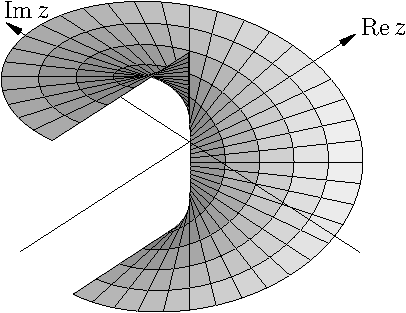
\includegraphics{figures/arggraph}
\caption{Graph of the principal branch of argument.\label{fig:arggraph}}
\end{myfig}

\begin{exbox}
\begin{exercise}
Show that $\Arg$ as defined above is not a continuous function on 
$\C \setminus \{ 0 \}$.
\end{exercise}
\end{exbox}

\subsection{Mapping properties of the exponential}

Let us see what the exponential does to the complex plane.
The identity $e^{z+w} = e^z e^w$ implies that the exponential
is never zero (exercise).
From the known properties of polar coordinates
and the real exponential, it follows that the complex exponential is
onto $\C \setminus \{ 0 \}$.
The complex exponential is not one-to-one, it is 
infinitely-many-to-one.  For any integer $k$,
\begin{equation} \label{eq:exponentialidentities}
e^{z+ik2\pi} = 
e^{z} e^{ik2\pi} =
e^z .
\end{equation}

\begin{exbox}
\begin{exercise} \label{exercise:exponetoonestrip}
Prove that \eqref{eq:exponentialidentities} are the only such identities by
showing that if $2k\pi < \Im z \leq 2(k+1)\pi$ and
$2k\pi < \Im w \leq 2(k+1)\pi$, then $e^z=e^w$ implies $z=w$.
\end{exercise}

\begin{exercise}%[\neededexmark]
Use $e^{z+w} = e^z e^w$ and $e^0 = 1 \not= 0$ to show that $e^z \not=0$ for all
$z \in \C$.  In other words, if a function $f$ satisfies $f(z+w)=f(z)f(w)$
and $f(0) = 1$, then $f(z) \not= 0$ for all $z$.
\end{exercise}
\end{exbox}

Consider a vertical line given by $x=c$.  As
\begin{equation*}
e^{z} = 
e^{x+iy} =
e^x e^{iy} ,
\end{equation*}
and $\sabs{e^{iy}} =1$, the exponential takes the vertical line $x=c$ to a
circle of radius $e^c$.  See \figureref{fig:expplotlines}.
Thus, the exponential takes the strip $a < x < b$ to the
annulus
\begin{equation*}
\bigl\{ z \in \C : e^a < \sabs{z} < e^b \bigr\} .
\end{equation*}

On the other hand, the horizontal line $y=c$
is taken to the ray from the origin to infinity where $\theta = c$ in polar
coordinates.  Again see \figureref{fig:expplotlines}.
Hence, the exponential takes the strip $a < y < b$ to the
sector
\begin{equation*}
\bigl\{ z \in \C : ``a < \arg z < b'' \bigr\} .
\end{equation*}
The reason for the quotation marks is that the inequality makes no
sense without interpreting it properly.  It means that one of the values
of $\arg z$ is between $a$ and $b$.
In particular, the exponential $e^z$ takes the set given by
$2k\pi < \Im z \leq 2(k+1)\pi$ in a one-to-one fashion
(see \exerciseref{exercise:exponetoonestrip})
onto $\C \setminus \{ 0 \}$.

\begin{myfig}
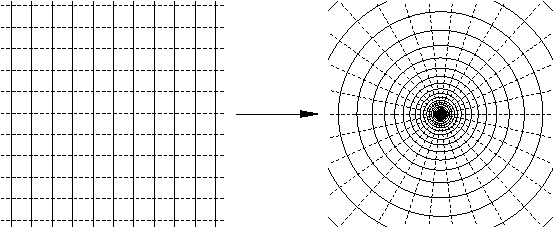
\includegraphics{figures/expplotlines}
\caption{Horizontal and vertical lines mapped by the exponential.  Note that
each horizontal line only goes to a ray from the
origin.\label{fig:expplotlines}}
\end{myfig}

%%%%%%%%%%%%%%%%%%%%%%%%%%%%%%%%%%%%%%%%%%%%%%%%%%%%%%%%%%%%%%%%%%%%%%%%%%%%%%

\section{The Riemann sphere}

It is sometimes useful to extend the real numbers by adding $\pm \infty$.
A similar concept exists for the complex plane, although
we only add one infinity.  We write
\glsadd{not:Cinfty}%
\glsadd{not:infty}%
\begin{equation*}
\C_{\infty} = \C \cup \{ \infty \} ,
\end{equation*}
and we call $\C_{\infty}$ the \emph{\myindex{Riemann sphere}}.
We want the topology of $\C_\infty$ to be the same as that of $\C$
when we are away from infinity.
Define the function $g \colon \C_\infty \to \C_\infty$ by
\begin{equation*}
g(z) =
\begin{cases}
\nicefrac{1}{z} & \text{if } z \not= 0 \text{ and } z \not= \infty, \\
\infty & \text{if } z = 0, \\
0 & \text{if } z = \infty.
\end{cases}
\end{equation*}
The function $g$ is bijective (one-to-one and onto).
Any neighborhood of the origin in $\C$ is taken to a set that
includes infinity and we call those the neighborhoods of
$\infty$.  When talking about a neighborhood of
infinity in $\C_{\infty}$, then we really want to think of this map,
and think of the corresponding neighborhood of the origin.

More concretely, we can give $\C_{\infty}$ a metric space structure.
Let $S^2$ be the unit sphere in $\R^3$,
that is, the set described by $x^2 + y^2 + z^2 = 1$ if $(x,y,z)$ are the
coordinates.\footnote{This is possibly the only instance in this book where
$z$ is a real number.}  The plane $\R^2$ with coordinates $(x,y)$ can be
identified with $\C$ with coordinate $\xi$ by taking $x+iy = \xi$.
Given any point $p \in S^2$ that is not the north pole $(0,0,1) \in S^2$,
there is a unique line in $\R^3$ through the point $(0,0,1)$ and $p$.
It is not difficult to prove that this line is never parallel to the
$xy$-plane, that is, to $\C$, and hence it must intersect $\C$ in a unique
point $\xi \in \C$ (a plane and a line intersect at a unique point unless
the two are parallel).  Define:
\begin{equation*}
\Phi(p) = \xi.
\end{equation*}
Let $\Phi\bigl((0,0,1)\bigr) = \infty$, so that we have a map
$\Phi \colon S^2 \to \C_\infty$.  This map is called the 
\emph{\myindex{stereographic projection}}.  See
\figureref{fig:riemannsphere}.
The map is bijective (exercise below),
and so define a metric on $\C_\infty$ by
using a metric on $S^2$, which can be the subspace
metric coming from the euclidean metric on $\R^3$.
Another possibility
could be the great circle distance, \exampleref{ms:greatcircle}, both
distances would lead to the same topology and so the same limits.

\begin{myfig}
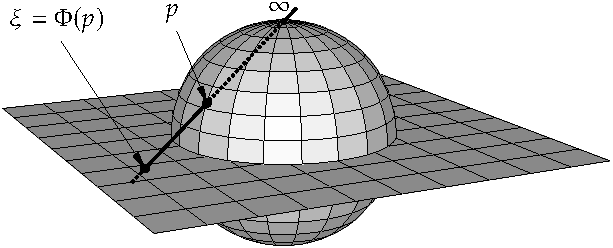
\includegraphics{figures/riemannsphere}
\caption{Stereographic projection of the Riemann sphere to the complex plane.\label{fig:riemannsphere}}
\end{myfig}

\begin{exbox}
\begin{exercise}%[\neededexmark]
Show that $\Phi$ is bijective.
\end{exercise}

\begin{exercise}
Suppose $(\phi,\theta)$
are spherical coordinates on $S^2$, where $0 \leq \phi \leq \pi$ is the zenith (angle made
with the $z$-axis) and $-\pi < \theta \leq \pi$ the azimuth, and we write
points in $\C$ using polar coordinates $re^{\theta}$.  Then prove that $\Phi$ of
$(\phi,\theta)$ is $\cot (\nicefrac{\phi}{2})\,e^{i\theta}$.
\end{exercise}

\begin{exercise}%[\neededexmark]
Show that the topology induced on $\C$ by the topology of $S^2$ using $\Phi$
as above is equivalent to the standard one.  That is, show that a set $U
\subset \C$
is open in the euclidean metric on $\C$ if and only if it is open using the
metric coming from $S^2$.
\end{exercise}
\end{exbox}

The point of the Riemann sphere is to give the value $\infty$ to certain
limits and to allow limits as $z$ tends to $\infty$.  For a
function $f \colon U \subset \C_\infty \to \C_\infty$, we define
\begin{equation*}
\lim_{z \to z_0} f(z) = L
\end{equation*}
as the metric space limit using the metric on the Riemann sphere, 
including
the cases when $z_0 = \infty$, $L = \infty$, or both.
Conveniently the Riemann sphere is compact.
Indeed, topologically, it is the same as the
\myquote{one-point compactification} of $\C$.

\begin{exbox}
\begin{exercise}%[\neededexmark]
Suppose $L \in \C$ and $z_0 \in \C$.
Show that $\lim_{z\to z_0} f(z) = L$ in the sense of the Riemann sphere
if and only if $\lim_{z \to z_0} f(z) = L$ in the usual sense (the euclidean
metric on $\C$).
\end{exercise}

\begin{exercise}%[\neededexmark]
Suppose $L \in \C$.
Show that $\lim_{z\to \infty} f(z) = L$ in the sense of the Riemann sphere
if and only if, for every $\epsilon > 0$ there exists an $M$ such that
$\sabs{f(z)-L} < \epsilon$ whenever $\sabs{z} > M$.
\end{exercise}

\begin{exercise}%[\neededexmark]
Suppose $z_0 \in \C$.
Show that $\lim_{z\to \infty} f(z) = \infty$ in the sense of the Riemann sphere
if and only if, for every $M > 0$ there exists a $\delta > 0$ such that
$\sabs{f(z)} > M$ whenever $\sabs{z-z_0} < \delta$.
\end{exercise}

\begin{exercise}%[\neededexmark]
Show that $\lim\limits_{z\to\infty} f(z) = L$ for some $L \in \C_\infty$ if and only if
$\lim\limits_{z \to 0} f(\nicefrac{1}{z}) = L$.
\end{exercise}

\begin{exercise}%[\neededexmark]
Show that $\lim\limits_{z\to z_0} f(z) = \infty$ for some $z_0 \in \C_\infty$ if and only if
$\lim\limits_{z \to z_0} \frac{1}{f(z)} = 0$.
\end{exercise}
\end{exbox}

It then makes sense to talk about the value of $\nicefrac{1}{z}$ at the origin
as $\infty$, and the value of $z$ at $\infty$ as $\infty$.
In fact, every nonconstant polynomial is $\infty$ at $\infty$.

\begin{exbox}
\begin{exercise}%[\neededexmark]
\label{exercise:polygoesinf}
Suppose $P(z) = a_d z^d + a_{d-1} z^{d-1} + \cdots + a_1 z + a_0$ is
a polynomial where $a_0,\ldots,a_d \in \C$.  Prove that if $d \geq 1$
and $a_d \not=0$ ($P$ is nonconstant),
then $\lim_{z \to \infty} P(z) = \infty$.
Hint: If $a_d = 1$, then using
$\abs{\frac{a_{d-1} z^{d-1} + \cdots + a_1 z + a_0}{z^d}}$, one finds
$\abs{P(z)} \geq \frac{1}{2} \sabs{z}^d$ for large $z$.
\end{exercise}
\end{exbox}

In calculus and in basic real analysis, you likely encountered
infinite limits in the sense of the extended reals.
Despite that the two types of infinite limits, either in the sense of the
extended reals or in the sense of the Riemann sphere,
look similar, and despite using essentially the same notation,
they are different.
For example,
\begin{equation*}
\lim_{x \to 0} \frac{1}{x} \quad \text{does not exist,} \qquad \text{but} \qquad
\lim_{z \to 0} \frac{1}{z} = \infty .
\end{equation*}
Here on the left-hand side we tacitly use the extended real sense
($x$ is real, no?) and on the
right-hand side we tacitly use the Riemann sphere sense ($z$ seems complex).
This could, obviously, cause confusion.
In this book, limits are going to be in the Riemann sphere sense
unless either otherwise noted or obvious.

\medskip

The arithmetic that one can 
reasonably define with the Riemann sphere $\infty$ is quite different from
the $\infty$ of the extended reals
(we may write the real infinity as $+\infty$ for emphasis).
No additions or subtractions make sense here.
Even something like
$\infty+\infty$ does not make sense, even though this is common for the
extended reals:  For instance, if $f(z) = z$ and $g(z) = -z$,
then $\lim_{z \to \infty} f(z) = \infty$,
$\lim_{z \to \infty} g(z) = \infty$, but $\lim_{z \to \infty}
\bigl(f(z)+g(z)\bigr) = 0$.
On the other hand, it is reasonable to define $\nicefrac{c}{0} = \infty$ for
$c \not= 0$, $\nicefrac{c}{\infty} = 0$ for $c \not= \infty$,
and $c \cdot \infty = \infty$ for $c \not= 0$.
Just make sure to definitely avoid doing any additions and subtractions of
infinities!

%%%%%%%%%%%%%%%%%%%%%%%%%%%%%%%%%%%%%%%%%%%%%%%%%%%%%%%%%%%%%%%%%%%%%%%%%%%%%%

\section{Linear fractional transformations}

A convenient set of transformations of the complex plane or the Riemann
sphere are the \emph{\myindex{linear fractional transformations}} (LFT)\index{LFT}
(sometimes called the \emph{\myindex{M\"obius transformations}}).
A function
\begin{equation*}
f(z) = \frac{a z + b}{c z + d}
\end{equation*}
is a linear fractional transformation if $ad \not= bc$.  The requirement on
$a$, $b$, $c$, $d$ guarantees that the ratio does not simplify and that the
function is nonconstant.

If $c\not=0$,
the expression is really defined only on
$\C \setminus \bigl\{ \nicefrac{-d}{c} \bigr\}$;
however, as in the last section, write
\begin{equation*}
f\left(\frac{-d}{c}\right) = \infty, \qquad \text{and} \qquad
f(\infty) = \frac{a}{c} .
\end{equation*}
If $c=0$, then set $f(\infty) = \infty$.  In either case, $f$ is a map of
the Riemann sphere to itself.

\begin{exbox}
\begin{exercise}%[\neededexmark]
Prove that an LFT is a bijective mapping of the Riemann sphere to itself.
\end{exercise}

\begin{exercise}%[\neededexmark]
Prove that an LFT extended to the Riemann sphere as above is continuous.
\end{exercise}
\end{exbox}

Any LFT is a composition of \emph{translations}\index{translation}
\begin{equation*}
T_a(z) = z + a ,
\end{equation*}
\emph{complex dilations}\index{complex dilation}
\begin{equation*}
D_a(z) = az ,
\end{equation*}
and \emph{inversions}\index{inversion}
\begin{equation*}
I(z) = \frac{1}{z}.
\end{equation*}
Consider an LFT $f(z) = \frac{az+b}{cz+d}$.
Without loss of generality, assume that either $c=1$ or $c=0$.
Suppose $c=1$ first,
\begin{equation*}
f(z)
=
\frac{a z + b}{z + d}
=
\frac{b-ad}{z+d}+a
=
T_a\biggr(D_{b-ad}\Bigr(I\bigl(T_d(z)\bigr)\Bigr)\biggr) .
\end{equation*}
If $c=0$, then we can also assume that $d=1$ and
so $f(z) = az + b$.
Then
\begin{equation*}
f(z) = az+b = T_b\bigl(D_a(z)\bigr) .
\end{equation*}

Translations are easy to understand, they just move the point.  Complex
dilation $D_a$ is the traditional euclidean plane-geometry dilation by $\sabs{a}$
and rotation by $\arg a$.  The inversion is the euclidean plane-geometry inversion
across the unit circle
and complex conjugation, see \figureref{fig:inversion}.  The euclidean
inversion across the circle simply inverts the distance to the origin:
\begin{equation*}
\frac{1}{\sabs{z}} e^{i \arg z} = 
\frac{\sabs{z}}{\sabs{z}^2} e^{i \arg z} = \frac{1}{\bar{z}} .
\end{equation*}
So to get our complex inversion $I(z)$ we also conjugate.

\begin{myfig}
\subimport*{figures/}{inversion.pdf_t}
\caption{Complex inversion.\label{fig:inversion}}
\end{myfig}

This sort of decomposition is quite useful in proving statements about
LFTs that are preserved under composition;
one only needs to prove them for $T_a$, $D_a$, and $I$.  This technique
will come in handy in just the next exercise.
Let us include straight lines in the set of circles.  After all, a straight
line is just a circle through infinity: Think about the circle of radius $r$
centered at $ir$ as $r \to \infty$.  Then an LFT takes circles to circles.
We leave this fact as an exercise.

\begin{exbox}
\begin{exercise}
Prove that if we include straight lines in the set of \myquote{circles,} then
an LFT takes circles to circles.
\end{exercise}

\begin{exercise} \label{exercise:anycircletorealline}
Prove that given any circle or a straight line, there exists an LFT
that takes that circle or line to the real line.
\end{exercise}
\end{exbox}

One way to view an LFT is as a $2 \times 2$ complex matrix.  For this purpose
we need to view the Riemann sphere as the so-called one-dimensional
\emph{\myindex{projective space}}.
Define the equivalence relation $\sim$ on $\C^2 \setminus \{ 0 \}$ by
$u \sim v$ if and only if $u = \lambda v$ for some $\lambda \in \C$.
The \emph{\myindex{one-dimensional complex projective}}
space is then defined by
\glsadd{not:CP1}%
\begin{equation*}
\C \bP^1
\overset{\text{def}}{=}
\faktor{\C^2 \setminus \{ 0\}}{\sim} \ .
\end{equation*}
In other words, $\C \bP^1$ is the set of \myquote{complex lines through the
origin} in $\C^2$, or yet in other words,
it is the set of one-dimensional vector
subspaces of $\C^2$.

We identify $\C\bP^1$ with $\C_\infty$ in the following
way.  Denote by
\glsadd{not:CP1pt}%
$[z:w] \in \C \bP^1$
the equivalence class (under $\sim$) of vectors in $\C^2$
that contains $(z,w) \in \C^2$.
Then define the map $\Psi \colon \C_\infty \to \C \bP^1$ as
\begin{equation*}
\Psi(z) =
\begin{cases}
[z:1] & \text{if } z \in \C , \\
[1:0] & \text{if } z=\infty .
\end{cases}
\end{equation*}

\begin{exbox}
\begin{exercise}
Prove that the $\Psi$ defined above is bijective.
\end{exercise}
\end{exbox}

Let us check that an LFT
\begin{equation*}
f(z) = \frac{a z + b}{c z + d}
\end{equation*}
corresponds to an invertible linear map given by the matrix
\begin{equation*}
M =
\begin{bmatrix}
a & b \\
c & d
\end{bmatrix} .
\end{equation*}
An invertible $M$ takes one-dimensional subspaces to one-dimensional
subspaces, so it sounds plausible.

First, $\Psi \circ f$ for $z \in \C \setminus \bigl\{ \nicefrac{-d}{c} \bigr\}$
is equal to
\begin{equation*}
\Psi \circ f(z) =
\left[\frac{a z + b}{c z + d}: 1 \right]
=
\left[a z + b: c z + d \right] ,
\end{equation*}
where the second inequality follows by definition of $\sim$.
When $z = \nicefrac{-d}{c}$, then $cz+d = 0$, or $f(0) = \infty$
and $\Psi(\infty) = [1:0] = [az+b : cz+d]$ as well.

Let us consider $\Psi \circ f \circ \Psi^{-1}$.
If $w \not= 0$, then $[z:w] = [ \nicefrac{z}{w}:1 ]$.  So
\begin{equation*}
\Psi \circ f \circ \Psi^{-1} \bigl([z:w]\bigr) =
\Psi \circ f \left(\frac{z}{w}\right) =
\left[a \frac{z}{w} + b : c \frac{z}{w} + d \right] =
\left[a z + b w: c z + d w \right] .
\end{equation*}
And one checks that the same equality holds if $w=0$.
As
$M \left[ \begin{smallmatrix} z \\ w \end{smallmatrix} \right]
= \left[ \begin{smallmatrix} 
a z + b w \\ c z + d w
\end{smallmatrix} \right]$,
the function $f$ corresponds to the linear map $v \mapsto Mv$ on $\C^2$.
The requirement $ad \not= bc$ implies $\det M \not= 0$,
or in other words, $M$ is invertible.
So every LFT is represented by an invertible $2 \times 2$ matrix $M$
(not uniquely), and
conversely every invertible $2 \times 2$ matrix $M$ corresponds to an LFT.

An invertible $2 \times 2$ matrix $M$ gives a map from
$\C^2 \setminus \{ 0 \}$ to $\C^2 \setminus \{ 0 \}$.
Let $\pi \colon \C^2 \setminus \{ 0 \} \to \C \bP^1$ be the map\footnote{The
\myquote{quotient map} or the \myquote{natural projection.}}
$\pi \bigl( (z,w) \bigr) =
[z:w]$.  The following commutative diagram\footnote{A diagram is
commutative if taking two different routes in the picture
gives the same map.}
may
illustrate the entire situation better:
\begin{equation*}
\begin{tikzcd}
\C^2 \setminus \{ 0 \} \arrow[r,"M"] \arrow[d,"\pi"] &
\C^2 \setminus \{ 0 \} \arrow[d,"\pi"] \\
\C \bP^1 \arrow[r,"\Psi \circ f \circ \Psi^{-1}"] \arrow[d,shift left,"\Psi^{-1}"] &
\C \bP^1 \arrow[d,shift left,"\Psi^{-1}"]
\\
\C_\infty \arrow[r,"f"]\arrow[u,shift left,"\Psi"] &
\C_\infty \arrow[u,shift left,"\Psi"]
\end{tikzcd}
\end{equation*}

\begin{example}
A handy LFT is the
\emph{\myindex{Cayley map}}:
\begin{equation*}
C(z)
=
\frac{z - i}{z + i} .
\end{equation*}
The map is clearly an LFT, and it
takes the upper half-plane $\bH = \{ z \in \C : \Im z > 0 \}$ to the
unit disc $\D$.  Let us see why.  The map takes $z \in \C$ to the unit disc if
\begin{equation*}
1 > \abs{\frac{z - i}{z + i} }
=
\frac{\sabs{z - i}}{\sabs{z + i}} .
\end{equation*}
In other words, $\sabs{z+i} > \sabs{z - i}$: The distance of $z$
to $-i$ is larger than the distance of $z$ to $i$.  It is straightforward
plane geometry to see this means that $z \in \bH$.  See
\figureref{fig:cayleydisc}.
\begin{myfig}
\subimport*{figures/}{cayleydisc.pdf_t}
\caption{Why does the Cayley map take $\bH$ to $\D$.\label{fig:cayleydisc}}
\end{myfig}
\end{example}

Any LFT is bijective if thought of as a map from $\C_\infty$
to itself, so $C^{-1}$ exists, and it is also a useful map.  We leave
it as an exercise to figure out the inverse.

\begin{exbox}
\begin{exercise}
Figure out what $C^{-1}$ (inverse of Cayley) is.  Hint: Think of $\C_\infty$ as $\C \bP^1$
and $C$ as a matrix.  It is really easy to invert $2 \times 2$ matrices.
\end{exercise}

\begin{exercise}
For every LFT $f(z) = \frac{az+b}{cz+d}$ find $f^{-1}$.
Hint: Same hint as above.
\end{exercise}
\end{exbox}

In the exercises, you have essentially just shown (or at least finished
showing) that LFTs form a group under composition,
called the \emph{\myindex{M\"obius group}}.
This group is generated by the elements
$T_a$, $D_a$, and $I$ for $a\in \C$.

%%%%%%%%%%%%%%%%%%%%%%%%%%%%%%%%%%%%%%%%%%%%%%%%%%%%%%%%%%%%%%%%%%%%%%%%%%%%%%

\section{Cross ratio \texorpdfstring{$\star$}{*}}

There is a certain quantity that is preserved by LFTs, the
\emph{\myindex{cross ratio}}:
\glsadd{not:crossratio}%
\begin{equation*}
(z_1,z_2;z_3,z_4)
=
\frac{(z_3-z_1)(z_4-z_2)}{(z_3-z_2)(z_4-z_1)}
=
\frac{z_3-z_1}{z_3-z_2} : 
\frac{z_4-z_1}{z_4-z_2} ,
\end{equation*}
where $z_1,z_2,z_3,z_4$ are complex numbers.  The cross ratio
was already described by the ancient Greeks\footnote{Pappus of Alexandria
lived in the early 4th century AD.  So it's not as impressively ancient as say
Thales's theorem from about a thousand years earlier.  Also, isn't
Alexandria in Egypt?}
and plays a key role in projective geometry.
The definition is extended to when one of the numbers is $\infty$ by simply
erasing the affected terms from the ratios.  For instance, if $z_1=\infty$,
then pretend that $z_3-\infty$
is really equal to $z_4-\infty$ and
thus they cancel---this makes sense as $\lim_{z\to\infty} \frac{z_3-z}{z_4-z} = 1$.
Consequently,
\begin{align*}
(\infty,z_2;z_3,z_4)
& =
\frac{z_4-z_2}{z_3-z_2}
,
&
(z_1,\infty;z_3,z_4)
& =
\frac{z_3-z_1}{z_4-z_1}
,
\\
(z_1,z_2;\infty,z_4)
& =
\frac{z_4-z_2}{z_4-z_1}
,
& 
(z_1,z_2;z_3,\infty)
& =
\frac{z_3-z_1}{z_3-z_2} .
\end{align*}

By \myquote{preserved by LFTs} we mean:

\begin{prop} \label{prop:crossratioinvariant}
Suppose that $f$ is an LFT, then
\begin{equation*}
(z_1,z_2;z_3,z_4) =
\bigl(f(z_1),f(z_2);f(z_3),f(z_4)\bigr) .
\end{equation*}
\end{prop}

\begin{exbox}
\begin{exercise}
Prove \propref{prop:crossratioinvariant}.
\end{exercise}

\begin{exercise}
Prove that four distinct points are on a line or a circle if and only if the cross
ratio is real.
Hint: See also \exerciseref{exercise:anycircletorealline}.
\end{exercise}
\end{exbox}

Cross ratios give a convenient way to describe LFTs.
For three distinct numbers $z_2,z_3,z_4$, the
function
\begin{equation*}
f(z) =
(z,z_2;z_3,z_4)
\end{equation*}
is an LFT such that $f(z_2) = 1$, $f(z_3)=0$ and $f(z_4) = \infty$.
In other words,
$(z,z_2;z_3,z_4) = 
\bigl(f(z),1;0,\infty\bigr)$.

\begin{exbox}
\begin{exercise}
Given two sets of distinct points $z_1,z_2,z_3 \in \C_\infty$
and $w_1,w_2,w_3 \in \C_\infty$, explicitly find an LFT $f$,
such that
$f(z_1) = w_1$,
$f(z_2) = w_2$, and
$f(z_3) = w_3$.
\end{exercise}

\begin{exercise}
Given distinct points $z_1,z_2,z_3 \in \C$ and
using the cross ratio definition of an LFT, explicitly find
the equation of a circle (or the straight line) through the three points.
Hint: Inverse image of the real line is a circle or a straight line.
\end{exercise}
\end{exbox}


%%%%%%%%%%%%%%%%%%%%%%%%%%%%%%%%%%%%%%%%%%%%%%%%%%%%%%%%%%%%%%%%%%%%%%%%%%%%%%
%%%%%%%%%%%%%%%%%%%%%%%%%%%%%%%%%%%%%%%%%%%%%%%%%%%%%%%%%%%%%%%%%%%%%%%%%%%%%%
%%%%%%%%%%%%%%%%%%%%%%%%%%%%%%%%%%%%%%%%%%%%%%%%%%%%%%%%%%%%%%%%%%%%%%%%%%%%%%

\chapter{Holomorphic and Analytic Functions} \label{ch:holanal}

\begin{myepigraph}
If this is coffee, please bring me some tea; but if this is tea, please bring me some coffee.

---Abraham Lincoln
\end{myepigraph}

%%%%%%%%%%%%%%%%%%%%%%%%%%%%%%%%%%%%%%%%%%%%%%%%%%%%%%%%%%%%%%%%%%%%%%%%%%%%%%

\section{Holomorphic functions and Cauchy--Riemann}
\label{sec:holfuncs}

\subsection{Holomorphic functions}

The functions we wish to study are those that in some sense
generalize polynomials in $z \in \C$;  we wish to study functions
that,
at least locally, behave like $P(z) = a_n z^n + a_{n-1} z^{n-1} + \cdots +
a_1 z + a_0$.  Polynomials are easy to understand and easy to work
with.  Alas, there aren't that many of them.  For instance, there is
no nonzero polynomial that solves the most basic of differential equations: $f' =
f$.  We must enlarge our horizons a bit.

Consider a polynomial $P(z)$ and expand it near some $z_0 \in \C$:
\begin{equation*}
P(z) = c_0 + c_1 (z-z_0) + c_2 {(z-z_0)}^2 + \cdots + c_n {(z-z_0)}^n .
\end{equation*}
In other words, $P(z_0+h) = c_0 + c_1 h + c_2 h^2 + \cdots + c_n h^n$.
Then
\begin{equation*}
\lim_{h \to 0} \frac{P(z_0+h) - P(z_0)}{h} =
\lim_{h \to 0} \frac{P(z_0+h) - c_0}{h} = c_1 .
\end{equation*}
So $P(z_0+h)$ is approximated (locally) by $c_0 + c_1 h$
up to an error that vanishes faster than $h$.
We should emphasize that the limits are as a complex $h$ goes to $0$.

Accordingly, we wish to study functions that are
locally approximated by $c_0 + c_1 h$ in the same way.  More formally,
we want functions such that
\begin{equation*}
f(z_0+h) = \underbrace{f(z_0)}_{c_0} + \underbrace{\xi h}_{c_1 h} + o(\sabs{h})
\end{equation*}
for some $\xi \in \C$, where
\glsadd{not:oofh}%
$o(\sabs{h})$ means any function of $h$
that goes to zero faster than $\sabs{h}$.

\begin{defn}
Suppose $U \subset \C$ is open.
Given $f \colon U \to \C$ and $z_0 \in U$, we say 
$f$ is \emph{\myindex{complex differentiable}} at $z_0$ if
the limit
\glsadd{not:cplxder}%
\begin{equation} \label{eq:complexdiff}
f'(z_0) \overset{\text{def}}{=}
\lim_{h \to 0} \frac{f(z_0+h) - f(z_0)}{h} \qquad ( = \xi )
\end{equation}
exists.
We call $f'(z_0)$ the \emph{\myindex{complex derivative}} of $f$
at $z_0$.  The notation
\glsadd{not:cplxderalt}%
 $\frac{df}{dz}$ is also useful.

A function $f \colon U \to \C$ is
\emph{\myindex{holomorphic}}
if it is complex differentiable at every point.  That is, if
\eqref{eq:complexdiff} exists for all $z_0 \in U$.
\end{defn}

Above, we proved the following proposition, which justifies our motivation
for the complex derivative.

\begin{prop}
If $P(z)$ is a polynomial, then $P \colon \C \to \C$ is holomorphic.
\end{prop}

The most basic result about holomorphic functions is that they are
continuous.
This can be proved either directly from the definition (exercise),
or using that a holomorphic function is
(real) differentiable as we will observe shortly.

\begin{prop} \label{prop:holiscont}
If $U \subset \C$ is open and $f \colon U \to \C$ is holomorphic, then $f$
is continuous.
\end{prop}

\begin{exbox}
\begin{exercise}
Directly from the definition of the complex derivative, show that a
holomorphic function is continuous (prove \propref{prop:holiscont}).
\end{exercise}

\begin{exercise}
Show that $f(z) = \bar{z}$ is not complex differentiable at any point.
\end{exercise}

\begin{exercise}
Show that $f(z) = z \bar{z} = \sabs{z}^2$ is complex differentiable
at the origin, but nowhere else.
\end{exercise}
\end{exbox}

\subsection{Cauchy--Riemann equations}

Suppose $U \subset \C$ is open, and
let $f \colon U \to \C$ be a
differentiable (in the real sense
and as a function of two real variables,
see \sectionref{sec:derinsv} in the appendix) function.
If we think of $\C$ as $\R^2$,
then the real derivative of $f$ is a $2 \times 2$ real matrix $D f$
that approximates $f$ locally.
That is, $f$ is (real) differentiable at $z_0$ if there exists
a $2 \times 2$ real matrix $Df|_{z_0}$ such that
\begin{equation*}
\lim_{h \to 0} \frac{\sabs{f(z_0+h) - f(z_0) - (Df|_{z_0}) h}}{\sabs{h}} = 0 .
\end{equation*}
We think of $h$ as a column vector in $\R^2$ 
to be able to apply it to the
$2 \times 2$ real matrix $Df|_{z_0}$.
A key point here is that the limit is taken
as $h$ moves in $\C$ (or $\R^2$ if you wish).
So $f(z_0+h) - f(z_0) - (Df|_{z_0}) h$ is $o(\sabs{h})$ as needed.
The trick is to see when $(Df|_{z_0}) h$ corresponds to $\xi h$
for some $\xi \in \C$.

Write $f = u+iv$, that is, as a
mapping into $\R^2$ it is $f = (u,v)$.  Then
\begin{equation*}
Df|_{z_0} =
\begin{bmatrix}
\frac{\partial u}{\partial x}\big|_{z_0} & \frac{\partial u}{\partial
y}\big|_{z_0} \\[5pt]
\frac{\partial v}{\partial x}\big|_{z_0} & \frac{\partial v}{\partial y}\big|_{z_0}
\end{bmatrix} .
\end{equation*}
We have seen in the last chapter that only a matrix of the form
$\left[ \begin{smallmatrix}
a & -b \\ b & a
\end{smallmatrix} \right]$ corresponds to multiplication a complex number $a+ib$.
Ergo, the derivative $Df|_{z_0}$ corresponds to multiplication by a
complex number only if it is of the form
$\left[ \begin{smallmatrix}
a & -b \\ b & a
\end{smallmatrix} \right]$, or in other words,
\begin{equation*}
\frac{\partial u}{\partial x}\Big|_{z_0} =
\frac{\partial v}{\partial y}\Big|_{z_0}
, \qquad
\frac{\partial v}{\partial x}\Big|_{z_0} =
-\frac{\partial u}{\partial y}\Big|_{z_0} .
\end{equation*}
In that event, $Df|_{z_0}$ corresponds to multiplication by the number
$\xi = \frac{\partial u}{\partial x}\big|_{z_0} + i \frac{\partial v}{\partial
x}\big|_{z_0}$, which is equal to
$\frac{\partial v}{\partial y}\big|_{z_0} - i \frac{\partial u}{\partial
y}\big|_{z_0}$.
Consequently,
\begin{equation*}
0 = \lim_{h \to 0} \frac{\sabs{f(z_0+h) - f(z_0) - \xi h}}{\sabs{h}} =
\lim_{h \to 0} \abs{\frac{f(z_0+h) - f(z_0)}{h} - \xi} ,
\end{equation*}
that is to say,
\begin{equation*}
\lim_{h \to 0} \frac{f(z_0+h) - f(z_0)}{h} = \xi .
\end{equation*}
So $f$ is complex differentiable at $z_0$ and $f'(z_0) = \xi$.

We proved that if $f$ is differentiable at $z_0$ (in the real sense), then 
the complex derivative exists at $z_0$ if and only if 
$\frac{\partial u}{\partial x}\big|_{z_0} = \frac{\partial v}{\partial
y}\big|_{z_0}$ and $\frac{\partial v}{\partial x}\big|_{z_0} = -\frac{\partial
u}{\partial y}\big|_{z_0}$.
By working backwards, it is immediate
that if $f$ is complex differentiable at $z_0$, then it is real
differentiable at $z_0$,
as the complex derivative $f'(z_0)$ gives the $Df|_{z_0}$.  Let us formalize
what we just proved.

\begin{prop}
Let $U \subset \C$ be open and $f = u+iv \colon U \to \C$ be a function.
Then
$f$ is complex differentiable at $z_0 \in U$
if and only if
$f$ (real) differentiable at $z_0 \in U$
with
$\frac{\partial u}{\partial x}\big|_{z_0} =
\frac{\partial v}{\partial y}\big|_{z_0}$
and
$\frac{\partial v}{\partial x}\big|_{z_0} =
-\frac{\partial u}{\partial y}\big|_{z_0}$ .
\end{prop}

If the partial derivatives exist and are continuous, then $f$ is
(real) differentiable (see \sectionref{sec:derinsv} again).
Thus we have the following, perhaps easier to apply, result
for continuously differentiable functions.

\begin{cor}
Let $U \subset \C$ be open and let $f = u+iv \colon U \to \C$ be a function
such that $\frac{\partial u}{\partial x}$, $\frac{\partial u}{\partial y}$, $\frac{\partial
v}{\partial x}$, and $\frac{\partial v}{\partial y}$ exist and are continuous (that is,
$f$ is continuously differentiable).
Then
\begin{equation} \label{eq:CReqreal}
\frac{\partial u}{\partial x} = \frac{\partial v}{\partial y} , \qquad
\frac{\partial v}{\partial x} = -\frac{\partial u}{\partial y}
\end{equation}
if and only if $f$ is complex differentiable at all $z \in U$, or in
other words, if
\begin{equation*}
f'(z) =
\lim_{h \to 0} \frac{f(z+h) - f(z)}{h}
\qquad
\text{exists for all $z \in U$.}
\end{equation*}
\end{cor}

The equations \eqref{eq:CReqreal} are called the
\emph{\myindex{Cauchy--Riemann equations}}\footnote{Interestingly,
the equations first appeared in the work of d'Alembert, and
it was Euler who first connected them to analytic functions.
Perhaps they had better be called the French-guy--German-guy equations,
except that Euler was really Swiss, he only lived in Germany for a long time.}.
Complex analysis, then, is the study of their solutions.

Hence, continuously differentiable functions that satisfy
the Cauchy--Riemann equations are holomorphic.
On the other hand,
a function that is complex differentiable everywhere (a holomorphic
function) is differentiable in the real sense,
and thus the partial derivatives exist and satisfy the Cauchy--Riemann
equations.  We will show later that holomorphic functions are
continuously differentiable---and not just differentiable, they are
infinitely differentiable.

\begin{exbox}
\begin{exercise} \label{exercise:exponentialholomorphic}
Show that the complex exponential function, and hence also sine and cosine,
is holomorphic, and show that $\exp' = \exp$.
\end{exercise}

\begin{exercise}
Let $U \subset \C$ be a domain (open and connected),
and $f \colon U \to \R$ be a real-valued function that is holomorphic.
Prove that $f$ is constant.
\end{exercise}

\begin{exercise}
Let $U \subset \C$ be open and $f \colon U \to \C$ holomorphic.
Write $f = u+iv$.  Show that $u$ and $v$ are \emph{\myindex{harmonic}},
that is,
$\frac{\partial^2 u}{\partial x^2} +  \frac{\partial^2 u}{\partial y^2} = 0$
and
$\frac{\partial^2 v}{\partial x^2} +  \frac{\partial^2 v}{\partial y^2} = 0$.
Feel free to assume that both $u$ and $v$ are twice continuously
differentiable.
\end{exercise}

\begin{exercise}
Let $U \subset \C$ be open and $f \colon U \to \C$ holomorphic.
Write $f = u+iv$.  Show that whenever the second derivative test applies 
to $u$ or $v$, you get a saddle, that is, prove that
$\frac{\partial^2 u}{\partial x^2} \frac{\partial^2 u}{\partial y^2}
-{\left(\frac{\partial^2 u}{\partial x \partial y}\right)}^2 \leq 0$
and
$\frac{\partial^2 v}{\partial x^2} \frac{\partial^2 v}{\partial y^2}
-{\left(\frac{\partial^2 v}{\partial x \partial y}\right)}^2 \leq 0$.
Feel free to assume that both $u$ and $v$ are twice continuously
differentiable.
\end{exercise}

\begin{exercise}
\begin{exparts}
\item
Show that in polar coordinates $z=re^{i\theta}$,
the Cauchy--Riemann equations (outside the origin) on $f=u+iv$ are
\begin{equation*}
\frac{\partial u}{\partial r} = \frac{1}{r} \frac{\partial v}{\partial \theta},
\qquad
\frac{\partial v}{\partial r} = \frac{-1}{r} \frac{\partial u}{\partial \theta}.
\end{equation*}
\item
Use the computation to (locally) find the form of all solutions to 
the Cauchy--Riemann equations where $\Re f = u$ does not depend on the
argument $\theta$.  By locally we mean only in some neighborhood $U$ of a
point $p \not= 0$.
\end{exparts}
\end{exercise}
\end{exbox}


%%%%%%%%%%%%%%%%%%%%%%%%%%%%%%%%%%%%%%%%%%%%%%%%%%%%%%%%%%%%%%%%%%%%%%%%%%%%%%

\section{Basic properties of holomorphic functions}

\subsection{Elementary calculus}

Let us solve a differential equation.  A common technique in analysis
to show an equality is to differentiate and then show that the derivative is
zero.

\begin{prop} \label{prop:zeroder}
Let $U \subset \C$ be a domain (open and connected),
and $f \colon U \to \C$ be holomorphic, and $f'(z) = 0$ for all $z \in U$.
Then $f$ is a constant.
\end{prop}

\begin{proof}
Follows from the standard real result,
see \thmref{thm:svzerodersol} in the appendix.
\end{proof}

\begin{prop}[Chain rule] \index{chain rule!complex derivative}
Let $U \subset \C$ and $V \subset \C$ be open, $f \colon U \to V$
complex differentiable at $z \in U$, and $g \colon V \to \C$ complex differentiable
at $f(z)$.  Then the composition $g \circ f$
is complex differentiable at $z$ and $(g \circ f)'(z) = g'\bigl(f(z)\bigr) f'(z)$.
\end{prop}

\begin{proof}
We offer two proofs.  The first works only for holomorphic
functions, and the second allow a generalization to nonholomorphic functions
with the Wirtinger operators in the next section (an exercise).

Let $h \not= 0$, and let $k = f(z+h) -f(z)$.  Then
\begin{equation*}
\begin{split}
\frac{(g \circ f)(z+h) - (g \circ f)(z)}{h}
& =
\frac{g \bigl( f(z+h) \bigr) - g\bigl( f(z) \bigr)}{f(z+h)-f(z)}
\frac{f(z+h)-f(z)}{h}
\\
& =
\frac{g \bigl( f(z) + k \bigr) - g\bigl( f(z) \bigr)}{k}
\frac{f(z+h)-f(z)}{h} .
\end{split}
\end{equation*}
A differentiable function is continuous, so $k \to 0$ as $h \to 0$.
The proof then follows by continuity of complex multiplication and taking
the limit as $h \to 0$.

Let's see the second proof.
Complex differentiable functions are real differentiable, so
we apply the standard real chain rule (\thmref{thm:realchain}).
Let $w = f(z) \in V$.  Then
\begin{equation*}
D(g \circ f)|_z = Dg|_w Df|_z .
\end{equation*}
The $2 \times 2$ matrices $Dg|_w$ and $Df|_z$ correspond to complex
numbers as $f$ and $g$ are both holomorphic.  A product $Dg|_w Df|_z$
of two such matrices again corresponds to a complex number, the product of
the two.
So $D(g \circ f)|_z$ corresponds to the pertinent complex number and $g \circ f$
complex differentiable at $z$, and the given equality holds.
\end{proof}

This simple statement of the chain rule still holds
if we plug a real differentiable function of one variable
into a complex differentiable
one.  If $\gamma \colon (a,b)
\to \C$ is a (real) differentiable function, where
$\gamma = \alpha + i \beta$,
then write $\gamma' = \alpha' + i \beta'$, which can also be interpreted
as a $2 \times 1$ matrix (column vector)
$\left[\begin{smallmatrix}\alpha'\\\beta'\end{smallmatrix}\right]$.

\begin{prop}[Chain rule]
\index{chain rule!composition of real and complex derivative}%
\label{prop:chainrule2}%
Let $U \subset \C$ be open,
$\gamma \colon (a,b) \to U$ (real) differentiable at $t \in (a,b)$,
and $f \colon U \to \C$ complex differentiable at $\gamma(t)$.
Then the composition $f \circ \gamma$ is (real) differentiable
at $t$ and $(f \circ \gamma)'(t) = f'\bigl(\gamma(t)\bigr) \gamma'(t)$.
\end{prop}

\begin{proof}
The first proof follows almost in the same way.  But it is useful to see
how we think of it in terms of real derivatives.
Let $z = \gamma(t)$.  Then 
\begin{equation*}
D(f \circ \gamma)|_{t} =
Df|_z D\gamma|_{t} .
\end{equation*}
That is an equation of real linear operators.  Now $Df|_z$ corresponds
to multiplication by the complex number $f'(z)$, and $D\gamma|_{t}$
is the $2 \times 1$ matrix (column vector) represented by $\gamma'(t)$.
The result follows.
\end{proof}

\begin{prop} \label{prop:sumproddiv}
Let $U \subset \C$ be open, and $f \colon U \to \C$ and
$g \colon U \to \C$ holomorphic.
\begin{enumerate}[(i)]
\item
$f+g$ is holomorphic and $\frac{d}{dz}\bigl[ f(z)+g(z) \bigr] = f'(z) + g'(z)$.
\item
$fg$ is holomorphic and $\frac{d}{dz}\bigl[f(z) g(z) \bigr] = f'(z)g(z) + f(z)g'(z)$.
\item
$\nicefrac{1}{g}$ is holomorphic on $\bigl\{ z \in U : g(z) \not= 0 \bigr\}$ and
$\frac{d}{dz}\bigl[\frac{1}{g(z)}\bigr] = \frac{-g'(z)}{{\bigl(g(z)\bigr)}^2}$.
\end{enumerate}
\end{prop}

The proof is left as an exercise below.  There are again several ways
to do it.  One way is almost identical to the
proof for functions of one real variable.
Note that
a holomorphic function is continuous, and so the set
$\bigl\{ z \in U : g(z) \not= 0 \bigr\}$ is open.

\begin{prop}[Power rule] \label{prop:powerrule}
\leavevmode
\begin{enumerate}[(i)]
\item For nonzero integers $n$, the function $z \mapsto z^n$ is holomorphic
where defined (outside the origin if $n$ negative) and $(z^n)' = n z^{n-1}$.
\item
A polynomial $P(z) = \sum_{n=0}^d c_n z^n$ is
holomorphic and
$P'(z) = \sum_{n=0}^{d-1} (n+1) c_{n+1} z^n$.
\item Rational functions $\frac{P(z)}{Q(z)}$
are holomorphic on the set where $Q$ is not zero.
\end{enumerate}
\end{prop}

The proof is again left as an exercise.

\begin{exbox}
\begin{exercise}
Prove \propref{prop:sumproddiv}.
Hint for product: 
$f(z+h)g(z+h) - f(z)g(z) =
f(z+h)g(z+h) - f(z)g(z+h) +
f(z)g(z+h) - f(z)g(z)$.
\end{exercise}

\begin{exercise}
Prove the first two items of \propref{prop:powerrule}.
Hint: For the power rule, first prove that $z$ is complex differentiable,
then prove $z^n$ is differentiable for positive $n$ (use product rule and
induction), and finally prove
that $z^n$ is differentiable for negative $n$.
Note: You are proving both that the complex derivative exists and
computing it.
\end{exercise}

\begin{exercise}
Prove the last two items of \propref{prop:powerrule}:
Polynonomials $P(z)$ are holomorphic on $\C$,
and rational functions
$\frac{P(z)}{Q(z)}$ is holomorphic on the set where $Q$ is nonzero.
\end{exercise}
\end{exbox}

Perhaps the reader may ask:
Is every solution to
the Cauchy--Riemann equations holomorphic?  Above, we saw that the answer
is affirmative for continuously differentiable functions, or at least
functions differentiable as functions of two variables.
Surprisingly, the answer is false%
\footnote{%
A good thorough account of this problem is:
J.\ D.\ Gray and  S.\ A.\ Morris,
\emph{When is a Function that Satisfies the Cauchy-Riemann Equations
Analytic?}  The American Mathematical Monthly, Vol.\ 85, No.\ 4 (Apr.,
1978), pp. 246--256.} if we only assume the existence of partial derivatives,
as the following exercise shows.

\begin{exbox}
\begin{exercise} \label{exercise:nonholCRsol}
Let $f(0) = 0$ and $f(z) = e^{-z^{-4}}$ for $z \not=0$.  Prove that partial
derivatives exist at every point (including the origin) and $f$
satisfies the Cauchy--Riemann equations at every point,
but $f$ is not complex differentiable at the origin ($f$ is not
even continuous).
\end{exercise}
\end{exbox}


\subsection{Wirtinger operators}

Suppose $z=x+iy$.
The so-called \emph{\myindex{Wirtinger operators}},
\begin{equation*}
\frac{\partial}{\partial z}
\overset{\text{def}}{=}
\frac{1}{2}
\left(
\frac{\partial}{\partial x} - i
\frac{\partial}{\partial y}
\right),
\qquad
\frac{\partial}{\partial \bar{z}}
\overset{\text{def}}{=}
\frac{1}{2}
\left(
\frac{\partial}{\partial x} + i
\frac{\partial}{\partial y}
\right)
,
\end{equation*}
provide a way to understand the
Cauchy--Riemann equations.\footnote{Despite the notation, these are
\emph{not} partial derivatives in $z$ and $\bar{z}$
(whatever that would mean).}
These operators are determined by insisting
\glsadd{not:wirt}%
\begin{equation*}
\frac{\partial}{\partial z} z = 1, \quad
\frac{\partial}{\partial z} \bar{z} = 0, \quad
\frac{\partial}{\partial \bar{z}} z = 0, \quad
\frac{\partial}{\partial \bar{z}} \bar{z} = 1.
\end{equation*}

The Cauchy--Riemann equations are then expressed as
\begin{equation} \label{eq:CReq}
\frac{\partial f}{\partial \bar{z}} = 0 .
\end{equation}
That seems a far nicer statement of the equations than \eqref{eq:CReqreal},
and it is just one complex equation.  
It says
a function is holomorphic if and only if it depends on $z$ but not on
$\bar{z}$.  That statement had better make no sense at first glance.
After all, the Wirtinger operators are not really derivatives with
respect to actual variables,
they are simply formal operators.
Also, and more importantly,
how could something possibly depend on $z$ but not on $\bar{z}$.
But let us humor ourselves and check what \eqref{eq:CReq} means:
\begin{equation*}
\frac{\partial f}{\partial \bar{z}} 
=
\frac{1}{2}
\left(
\frac{\partial f}{\partial x} + i
\frac{\partial f}{\partial y}
\right)
=
\frac{1}{2}
\left(
\frac{\partial u}{\partial x} 
+ i \frac{\partial v}{\partial x} 
+ i \frac{\partial u}{\partial y}
- \frac{\partial v}{\partial y}
\right) 
=
\frac{1}{2}
\left(
\frac{\partial u}{\partial x} 
- \frac{\partial v}{\partial y}
\right)
+
\frac{i}{2}
\left(
\frac{\partial v}{\partial x} 
+ \frac{\partial u}{\partial y}
\right) .
\end{equation*}
This expression is zero if and only if the real and imaginary
parts are zero.  Namely,
\begin{equation*}
\frac{\partial u}{\partial x} 
- \frac{\partial v}{\partial y}
= 0,
\qquad
\text{and}
\qquad
\frac{\partial v}{\partial x} 
+ \frac{\partial u}{\partial y} = 0
.
\end{equation*}
That is, the Cauchy--Riemann equations are satisfied.  For emphasis,
we state this result as a proposition.

\begin{prop}
\label{prop:WirtCR}
Let $U \subset \C$ be open.  Then $f \colon U \to \C$ is
holomorphic if and only if
$f$ is (real) differentiable and
\begin{equation*}
\frac{\partial f}{\partial \bar{z}} \equiv 0 .
\end{equation*}
\end{prop}


The Wirtinger derivative in $z$ computes the holomorphic derivative
if $f$ is holomorphic.  We can write
the $z$ derivative in two different ways:
\begin{equation*}
\begin{split}
\frac{\partial f}{\partial z} 
=
\frac{1}{2}
\left(
\frac{\partial u}{\partial x} 
+ \frac{\partial v}{\partial y}
\right)
+
\frac{i}{2}
\left( \frac{\partial v}{\partial x} - \frac{\partial u}{\partial y}
\right) 
& =
\frac{\partial u}{\partial x} 
+ i \frac{\partial v}{\partial x}
 =
\frac{\partial f}{\partial x}
\\
& =
\frac{1}{i} \left(
\frac{\partial u}{\partial y}
+ i
\frac{\partial v}{\partial y} 
\right)
 =
\frac{1}{i}
\frac{\partial f}{\partial y}
.
\end{split}
\end{equation*}
In the second form, we want to think of the derivative in
the imaginary direction as a derivative in $iy$ and not the partial
derivative in $y$.  That is why the $\nicefrac{1}{i}$ is there.
If $f$ is complex differentiable, $h$ can
approach zero from every direction:
\begin{equation*}
f'(z) =
\lim_{\substack{h \to 0\\h\in\C}}
\frac{f(z+h)-f(z)}{h}
=
\lim_{\substack{t \to 0\\t\in\R}}
\frac{f(z+t)-f(z)}{t}
=
\frac{\partial u}{\partial x} \Big|_z
+ i \frac{\partial v}{\partial x}\Big|_z
 =
\frac{\partial f}{\partial x} \Big|_z ,
\end{equation*}
and
\begin{equation*}
f'(z) =
\lim_{\substack{h \to 0\\h\in\C}}
\frac{f(z+h)-f(z)}{h}
=
\lim_{\substack{t \to 0\\t\in\R}}
\frac{f(z+it)-f(z)}{it}
=
\frac{1}{i}
\left(
\frac{\partial u}{\partial y}  \Big|_z
+ i \frac{\partial v}{\partial y} \Big|_z
\right)
 =
\frac{1}{i}
\frac{\partial f}{\partial y} \Big|_z .
\end{equation*}
So for a holomorphic function
\begin{equation*}
f' =
\frac{\partial f}{\partial z} .
\end{equation*}

The complex derivative $f'$, sometimes written as $\frac{df}{dz}$,
only exists for holomorphic functions.
The Wirtinger operators
$\frac{\partial f}{\partial z}$ and
$\frac{\partial f}{\partial \bar{z}}$ make sense for every real differentiable
function.
Do not confuse the notation
even though $\frac{df}{dz}$ and 
$\frac{\partial f}{\partial z}$ look similar.
Consider a polynomial $P$ in $x$ and $y$, or equivalently
in $z$ and $\bar{z}$.\footnote{Usually when we say \myquote{polynomial} in this
book, we mean a polynomial in $z$, so we will always explicitly mention
if we mean a polynomial in $x$ and $y$, or $z$ and $\bar{z}$.}
The Wirtinger operators exist and
work as if $z$ and $\bar{z}$ really were independent variables.  For example:
\begin{equation*}
\frac{\partial}{\partial z}
\left[ z^2 \bar{z}^3 + z^{10} \right]
=
2z \bar{z}^3 + 10 z^{9}
\qquad
\text{and}
\qquad
\frac{\partial}{\partial \bar{z}}
\left[ z^2 \bar{z}^3 + z^{10} \right]
=
z^2 ( 3 \bar{z}^2 ) + 0 .
\end{equation*}
So at least for polynomials, a function is holomorphic 
if it does not depend on $\bar{z}$.
However, the function $z^2 \bar{z}^3 + z^{10}$ is not holomorphic
and
$\frac{d}{dz} \bigl[ z^2 \bar{z}^3 + z^{10} \bigr]$
does not exist.

\begin{exbox}
\begin{exercise}
Justify the statement about Wirtinger operators:  Consider
the function $z^m\bar{z}^n$ for any nonnegative integrers $m$ and $n$.
Compute
$\frac{\partial}{\partial z} \left[ z^m\bar{z}^n \right]$
and
$\frac{\partial}{\partial \bar{z}} \left[ z^m\bar{z}^n \right]$.
\end{exercise}

\begin{exercise}
Let $f \colon U \subset \C \to \C$ be real differentiable at $p \in U$.
The derivative $Df|_{p}$ can be represented by two numbers $\xi$ and
$\zeta$: It is the real linear map $h \mapsto \xi h + \zeta \bar{h}$
(see \exerciseref{exercise:reallinmap}).
Show that $\frac{\partial f}{\partial z} \big|_p = \xi$ and
$\frac{\partial f}{\partial \bar{z}} \big|_p = \zeta$.
\end{exercise}

\begin{exercise}
Prove that $ix^2 - 2xy -iy^2 + 3x + 3iy + i$ is a holomorphic function of
$z = x+iy$, not by
differentiating, but by writing as a polynomial in $z$ and not $\bar{z}$.
That is, write $x$ and $y$ in terms of $z$ and $\bar{z}$, and then show
that $\bar{z}$ cancels.
\end{exercise}

\begin{exercise}%[\optneededexmark]
\label{exercise:wirtingerandbar}
Suppose $f \colon U \to \C$ is real differentiable and let $\bar{f}$
denote the complex conjugate of $f$.  Show
\begin{equation*}
\overline{\left(\frac{\partial f}{\partial z}\right)} = 
\frac{\partial \bar{f}}{\partial \bar{z}}
\qquad \text{and} \qquad
\overline{\left(\frac{\partial f}{\partial \bar{z}}\right)} = 
\frac{\partial \bar{f}}{\partial z} .
\end{equation*}
\end{exercise}

\begin{exercise}
Suppose $f \colon U \to \C$ is such that both $f$ and its conjugate
$\bar{f}$ is holomorphic.  Show that $f$ is constant.
\end{exercise}

\begin{exercise}%[\optneededexmark]
\label{exercise:wirtingerchain}
Prove a Wirtinger operator version of
the chain rule\index{chain rule!Wirtinger operators}
for real differentiable
functions:  Let $U \subset \C$ and $V \subset \C$ be open, and $f \colon U \to V$
(real) differentiable at $p \in U$, $g \colon V \to \C$ (real) differentiable
at $f(p) \in V$.  Write $\bar{f}$ for the function that is the complex conjugate
of $f$.  Then the composition $g \circ f$
is (real) differentiable at $p$ and
\begin{equation*}
\frac{\partial (g \circ f)}{\partial z}\Big|_p
=
\frac{\partial g}{\partial z}\Big|_{f(p)}
\frac{\partial f}{\partial z}\Big|_p
+
\frac{\partial g}{\partial \bar{z}}\Big|_{f(p)}
\frac{\partial \bar{f}}{\partial z}\Big|_p ,
\end{equation*}
and
\begin{equation*}
\frac{\partial (g \circ f)}{\partial \bar{z}}\Big|_p
=
\frac{\partial g}{\partial z}\Big|_{f(p)}
\frac{\partial f}{\partial \bar{z}}\Big|_p
+
\frac{\partial g}{\partial \bar{z}}\Big|_{f(p)}
\frac{\partial \bar{f}}{\partial \bar{z}}\Big|_p .
\end{equation*}
Remark: This almost makes it seem like a nonholomorphic function is a
function of not just $z$, but two \myquote{independent} variables $z$ and
$\bar{z}$.
\end{exercise}

\begin{exercise}
A function satisfying $\frac{\partial f}{\partial z} = 0$ is called
\emph{\myindex{antiholomorphic}}.
Suppose $U \subset \C$ is open and $f \colon U \to \C$.
Prove that if the following
limit exists
\begin{equation*}
g(z) = 
\lim_{h \to 0}
\frac{f(z+h)-f(z)}{\bar{h}}
\end{equation*}
for all $z \in U$ (note the bar on the $h$), then $f$ is real differentiable, and satisfies
\begin{equation*}
\frac{\partial f}{\partial z} \equiv 0, \qquad \text{and} \qquad
\frac{\partial f}{\partial \bar{z}}\Big|_{p} = g(p).
\end{equation*}
\end{exercise}

\begin{exercise}
\begin{exparts}
\item
Suppose $U \subset \C$ is open and $f \colon U \to \C$
is holomorphic.  Show that if $\frac{\partial f}{\partial z}$ is
continuous, then $\frac{\partial f}{\partial x}$ and
$\frac{\partial f}{\partial y}$ are continuous.
\item
Find an example of a function $f \colon \C \to \C$ for which 
$\frac{\partial f}{\partial x}$ and 
$\frac{\partial f}{\partial y}$ exist at all points,
$\frac{\partial f}{\partial z}$ is continuous, but
$\frac{\partial f}{\partial x}$ and
$\frac{\partial f}{\partial y}$ are discontinuous.
Hint: Consider the conjugate of the function from
\exerciseref{exercise:nonholCRsol}.
\end{exparts}
\end{exercise}
\end{exbox}

\subsection{Inverse function theorem and automorphisms}

To work with a new category of functions, one should always ask
what are the right changes of variables.

\begin{defn}
Let $U, V \subset \C$ be open sets.
A holomorphic function $f \colon U \to V$ that is bijective and
such that the inverse $f^{-1}$ is also holomorphic\footnote{%
Surprisingly, we will (later) show that this condition is superfluous.}
is called a
\emph{\myindex{biholomorphism}}.
If there exists a biholomorphism $f \colon U \to V$, we say that
$U$ and $V$ are \emph{\myindex{biholomorphic}}.
If $U = V$, then a biholomorphism $f$ is called an
\emph{\myindex{automorphism}}\footnote{%
The word automorphism is used in other contexts as well, it always means
that it maps the set to itself and
is the right sort of equivalence in the context you are in.
In topology it means a homeomorphism, in differential geometry a
diffeomorphism, in group theory an isomorphism.}.
Let $\operatorname{Aut(U)}$ denote the set of all automorphisms of $U$.
Traditionally,
a biholomorphism
$f \colon U \to V$ is called a \emph{\myindex{conformal mapping}} and
then $U$ and $V$ are said to be
\emph{\myindex{conformally equivalent}}.\footnote{In one complex variable only!
In higher dimensions the definitions differ.}
\end{defn}

For example, the Cayley map
$C(z)
=
\frac{z - i}{z + i}$
takes the upper half-plane
$\bH = \{ z \in \C : \Im z > 0 \}$ to the unit disc $\D$ and
has a holomorphic inverse.
In other words, $C|_{\bH} \colon \bH \to \D$ is a biholomorphism
making $\bH$ and $\D$ biholomorphic.

The reader can check that for a nonempty open $U \subset \C$, the set
$\operatorname{Aut}(U)$ is a group under
composition, although we will not be too worried about the group
structure.

\begin{exbox}
\begin{exercise}
Check that
$\operatorname{Aut(U)}$ is a group under composition:
Composition of two automorphisms is an automorphism,
there is an identity element,
composition is associative,
and there exists an inverse for every element.
\end{exercise}

\begin{exercise}
Show that for any constants $a,b \in \C$, $a \not= 0$, the function
$a z + b$ is an automorphism of $\C$.
\end{exercise}
\end{exbox}

A biholomorphism $f$ has the property that $f'(z) \not= 0$ for all $z$.
Indeed,
$f$ and $f^{-1}$ are holomorphic, so differentiate the
equality
$f^{-1}\bigl(f(z)\bigr) = z$ using the chain rule to find
$(f^{-1})' \bigl(f(z)\bigr) f'(z) = 1$.  Hence, $f'(z)$ cannot be zero.
If $w = f(z)$, then
\begin{equation*}
(f^{-1})'(w) = \frac{1}{f'(z)}
\qquad \text{or} \qquad
f'(z) =
\frac{1}{(f^{-1})'(w)} .
\end{equation*}

Locally, the relationship between nonzero derivative and invertibility is
the inverse function theorem.  Consider a holomorphic function
$f = u+iv$, its real derivative $Df$, and its complex derivative $f'$.
The real derivative as a matrix is
\begin{equation*}
Df =
\begin{bmatrix}
\frac{\partial u}{\partial x} & \frac{\partial u}{\partial y} \\[5pt]
\frac{\partial v}{\partial x} & \frac{\partial v}{\partial y}
\end{bmatrix} ,
\end{equation*}
so using the Cauchy--Riemann equations, we compute the Jacobian determinant,
\begin{equation*}
\det Df =
\frac{\partial u}{\partial x}
\frac{\partial v}{\partial y} -
\frac{\partial u}{\partial y} 
\frac{\partial v}{\partial x}
=
{\left(\frac{\partial u}{\partial x}\right)}^2
+
{\left(\frac{\partial v}{\partial x}\right)}^2
=
\abs{f'(z)}^2 .
\end{equation*}
The Jacobian determinant is nonzero (positive) and $Df$ is invertible
whenever $f'(z)$ is nonzero.
Among other things this computation
implies that the determinant of
$Df$ is always nonnegative, so a holomorphic function preserves orientation.

The real inverse function theorem (\thmref{thm:inverse})
for continuously differentiable
functions of $\R^2$ to $\R^2$
says that if $Df$ is invertible at some point $p$, then $f$ takes a
neighborhood $V$ of $p$ bijectively to a neighborhood $f(V)$
of $f(p)$ and the inverse on that neighborhood is continuously
differentiable with $D(f^{-1})|_{f(p)} = (Df|_p)^{-1}$.

An inverse of a $2 \times 2$ matrix that represents a complex number also
represents a complex number (the reciprocal).  So if $f$
satisfied the Cauchy--Riemann equations, so does the inverse.  We 
instantly obtain the holomorphic inverse function theorem.

\begin{thm}[Inverse function theorem for holomorphic functions]
\index{inverse function theorem!holomorphic functions}
\label{thm:inversehol}
Suppose $U \subset \C$ is open, $f \colon U \to \C$ is holomorphic,
$p \in U$, and $f'(p) \not= 0$.  Suppose further that $f$ is continuously
differentiable.
Then there exist open sets $V, W \subset \C$ such that
$p \in V \subset U$, $f(V) = W$, the restriction $f|_V$ is injective
(one-to-one),
and hence a $g \colon W \to V$ exists such that
$g(y) = (f|_V)^{-1}(y)$.
Furthermore, $g$ is holomorphic and
\begin{equation*}
g'(w) = \frac{1}{f'\bigl(g(w)\bigr)} \qquad \text{for all $w \in W$}.
\end{equation*}
\end{thm}

The hypothesis that $f$ is continuously differentiable is completely
superfluous.\footnote{Cauchy (early 1800s)
assumed continuity of the derivative for his work.
It was Goursat more than half a century later that showed that continuity of the
derivative came for free.}
Every holomorphic function is continuously
differentiable, although you will have to wait till around
\thmref{thm:holfuncinfder} for why that is true.

A holomorphic function whose derivative is nonzero
everywhere need not be globally invertible.  The exponential $e^z$
is never zero, and thus neither is its derivative.  However, $e^{z} = e^{z+2\pi i}$,
so the
exponential is not injective.
That the inverse of the
exponential, the logarithm,
has infinitely many values at each point is fundamental to complex analysis.
So much so that we've named a whole chapter after the logarithm.

Another interesting remark about biholomorphisms is that generally
there are very few biholomorphisms for a specific open sets $U$ and $V$.  We will
compute later the automorphism group of a few sets such as the disc or the
complex plane, and it is in fact rather small.
For instance, automorphisms of $\C$ are simply the affine maps $a
z + b$.  On the other hand, at each point, there are a huge number of
holomorphic functions with nonzero derivative.  So there are lots of local
coordinate changes, but few global coordinate changes.

In the following exercises, you may want to apply the inverse
function theorem to show that the inverse is holomorphic.

\begin{exbox}
\begin{exercise}
\begin{exparts}
\item
Find a biholomorphism from the horizontal strip
$S = \{ z \in \C : 0 < \Im z < \pi \}$ to
the upper half-plane $\bH = \{ z \in \C : \Im z > 0 \}$.
\item
Find a biholomorphism from the horizontal strip
$S$ to the unit disc $\D$.
\end{exparts}
\end{exercise}

\begin{exercise}
\pagebreak[2]
\begin{exparts}
\item
Show that $z^2$ is 2-to-1 on $\C \setminus \{ 0 \}$ while its
derivative is nonzero.
\item
Show that $z^2$ is a biholomorphism of the right half-plane
$\{ z \in \C : \Re z > 0 \}$
and the slit plane $\C \setminus (-\infty,0] = \{ z \in \C : \Im z \not= 0 \text{ or } \Re z > 0 \}$.
\end{exparts}
\end{exercise}

\begin{exercise} \label{exercise:segmentcomplement}
Consider $f(z) = z+ \nicefrac{1}{z}$.  Show that $f$ takes $\C \setminus
\overline{\D}$ biholomorphically to $\C \setminus [-2,2]$, and it also takes
$\D \setminus \{ 0 \}$ biholomorphically to $\C \setminus [-2,2]$.
\end{exercise}

\begin{exercise}
Consider $\Delta_1$ a closed disc of radius 1 centered at $i$ and $\Delta_2$ a closed disc of radius 1 centered $-i$.
Find a biholomorphism of $\C \setminus (\Delta_1 \cup \Delta_2)$
onto the unit disc.
Hint: Figure out what $\nicefrac{1}{z}$ does to the two circles.
\end{exercise}

\begin{exercise}
Let $f(z) = \frac{1-z^4}{1+z^4}$ and $g(z) = i {\left( \frac{1-z^2}{1+z^2}
\right)}^2$.  Let $S = \{ z \in \C : \sabs{z} < 1, \Re z > 0, \Im z > 0 \}$.
Find $f(S)$ and $g(S)$.  Then show that they are both biholomorphisms onto their
image.  Think about the functions as composition.
\end{exercise}

\begin{exercise}
\begin{exparts}
\item
Show that if $\Delta \subset \C$ is a disc such that $0 \notin \Delta$, then
there exist two distinct holomorphic functions $f \colon \Delta \to \C$ such that
${\bigl(f(z)\bigr)}^2 = z$.  In other words, $f(z) = \pm \sqrt{z}$ and the
square root and its negative is holomorphic on $\Delta$.
\item
Show that there does not exist a continuous $f \colon \C \setminus \{ 0 \} =
\C$ such that ${\bigl(f(z)\bigr)}^2 = z$.  That is, we cannot choose a
continuous square root in the punctured plane.  Hint: Just consider the unit
circle.
\end{exparts}
\end{exercise}

\begin{exercise}
\begin{exparts}
\item
Suppose $f$ is antiholomorphic, that is assume $f$ is (real) differentiable
and $\frac{\partial f}{\partial z} = 0$.  Show that
$\det Df\big|_p = - \babs{\frac{\partial f}{\partial \bar{z}}(p)}^2$.  In other words,
the Jacobian determinant is nonpositive, and $f$ flips orientation.
\item
More generally, if $f$ is (real) differentiable, then
$\det Df\big|_p = \babs{\frac{\partial f}{\partial z}(p)}^2 -
\babs{\frac{\partial f}{\partial \bar{z}}(p)}^2$.
\end{exparts}
\end{exercise}
\end{exbox}

\subsection{Conformality \texorpdfstring{$\star$}{*}}

The actual definition of \myquote{conformal mapping} is 
a (real) differentiable bijective mapping $f \colon U \to V$ of open
$U, V \subset \R^2$ that preserves
a)~orientation, and b)~angles.
Both of these are taken in the infinitesimal sense, that is, they are
statements about $Df$.  Consider two continuously differentiable curves
$\gamma \colon (-\epsilon,\epsilon) \to \R^2$ and
$\alpha \colon (-\epsilon,\epsilon) \to \R^2$, such that
$\gamma(0)=\alpha(0) = p \in \R^2$.  By preserving angles, we
mean that the curves $f \circ \gamma$ and $f \circ \alpha$ meet at the same
angle at $f(p)$, see \figureref{fig:conform}.  In other words,
\begin{equation*}
\text{angle between } Df|_p \gamma'(0) \text{ and }
Df|_p \alpha'(0)
\quad = \quad
\text{angle between } \gamma'(0) \text{ and } \alpha'(0) .
\end{equation*}
As we are preserving orientation,
we can take the angle to be the signed angle starting at one vector and
ending at the other vector. 

\begin{myfig}
\subimport*{figures/}{conform.pdf_t}
\caption{Preserving angles (and orientation).\label{fig:conform}}
\end{myfig}

By preserving angles we also mean that no vector can be taken to zero,
as zero does not make any well-defined angle with anything else.
Thus $Df$ must be invertible at every point for a conformal map.
We are really just doing linear algebra, so let us see the relevant
linear algebra statement.

\begin{prop}
A $2\times 2$ real matrix $M$
preserves orientation and angles
if and only if $M$ corresponds to the multiplication by a nonzero
complex number.
\end{prop}

\begin{proof}
Suppose that $M$ preserves orientation and angles.
As we said $M$ must be nonsingular.
Let $M =
\left[\begin{smallmatrix}a&b\\c&d\end{smallmatrix}\right]$.
As $M$ preserves angles, given two vectors $v$ and
$w$ in $\R^2$, the angle between $Mv$ and $Mw$ is the same as the angle
between $v$ and $w$.
The vectors
$v=\left[\begin{smallmatrix}1\\0\end{smallmatrix}\right]$ and
$w=\left[\begin{smallmatrix}0\\1\end{smallmatrix}\right]$ are
orthogonal, and so $Mv$ and $Mw$ are orthogonal:
\begin{equation*}
0 = Mv \cdot Mw = 
\begin{bmatrix} a\\c \end{bmatrix}
\cdot
\begin{bmatrix} b\\d \end{bmatrix}
=
ab+cd .
\end{equation*}
As $M$ is nonsingular, either $a$ or $c$ is nonzero.  In either case,
there must exist some nonzero $r \in \R$ such that
\begin{equation*}
M =
\begin{bmatrix}
a &-rc \\
c & ra
\end{bmatrix} .
\end{equation*}
A similar calculation using
$v=\left[\begin{smallmatrix}1\\1\end{smallmatrix}\right]$ and
$w=\left[\begin{smallmatrix}1\\-1\end{smallmatrix}\right]$ results in
$a^2+c^2 = b^2+d^2 = r^2(a^2+c^2)$.  Or in other words $r=\pm 1$.
That $M$ preserves orientation means $\det M > 0$.
As $\det M = r(a^2+c^2)$, we find $r=1$.
Hence,
\begin{equation*}
M =
\begin{bmatrix}
a & -c \\
c &  a
\end{bmatrix} .
\end{equation*}
In other words, $M$ corresponds to multiplication by the complex number
$a+ic$.

For the converse, assume $M$ is multiplication by the
nonzero complex number~$\xi$.
Let
$z = \sabs{z} e^{i\theta}$ and $w = \sabs{w} e^{i\psi}$ be two nonzero
complex numbers, thinking of them as vectors in $\R^2$.
The (signed) angle between them, $\theta-\psi$, can be
computed using
\begin{equation*}
\frac{z\bar{w}}{\sabs{z}\sabs{w}}
=
e^{i(\theta-\psi)} .
\end{equation*}
Similarly the angle between 
$\xi z$ and $\xi w$ can be computed using
\begin{equation*}
\frac{\xi z\overline{\xi w}}{\sabs{\xi z}\sabs{\xi w}} 
=
\frac{\sabs{\xi}^2 z\overline{w}}{\sabs{\xi}^2 \sabs{z}\sabs{w}} 
=
\frac{z\overline{w}}{\sabs{z}\sabs{w}} = e^{i(\theta-\psi)}.
\end{equation*}
So the (signed) angle is the same, and multiplication by $\xi$ preserves
orientation and angles.
\end{proof}

Another way to see that if $M$ is multiplication by $\xi$, then
$M$ preserves orientation is to note that
$\det M = \sabs{\xi}^2 > 0$.

Applying the proposition to $Df$ we find:

\begin{cor}
Let $U \subset \C$ be open.
A real differentiable function $f \colon U \to \C$
preserves orientation and angles
if and only if $f$ is holomorphic and $f'$ never vanishes.
\end{cor}

In other words, conformal maps are holomorphic, and holomorphic
maps with nonzero derivative preserve angles and orientation.
Once we prove later that
holomorphic maps are continuously differentiable and we will be able to
apply the inverse function theorem we have just presented in the previous
subsection, then we will see that conformal maps are also biholomorphic.

\begin{exbox}
\begin{exercise}
Prove that a $2 \times 2$ matrix $M$ preserves angles and reverses
orientation if and only if $M$ corresponds to the mapping $h \mapsto \xi
\bar{h}$ for some $\xi \in \C$.
\end{exercise}

\begin{exercise}
Let $U \subset \C$ be open.
Prove that real differentiable function $f \colon U \to \C$ preserves angles
and reverses orientation if and only if the conjugate $\bar{f}$ is
holomorphic and its derivative never vanishes.
\end{exercise}
\end{exbox}

%%%%%%%%%%%%%%%%%%%%%%%%%%%%%%%%%%%%%%%%%%%%%%%%%%%%%%%%%%%%%%%%%%%%%%%%%%%%%%

\section{Power series}
\label{sec:powerser}

\subsection{The function \texorpdfstring{$z^n$}{z to the n}}

To understand holomorphic functions locally, 
it is sufficient to understand $z \mapsto z^n$.  We will prove that
holomorphic functions are just power series and so we can always factor
a $z^n$ for some $n$ out of a power series that vanishes at the origin,
which is, after all, just a sum of such terms.  This means that every holomorphic
function really behaves like $z^n$ behaves near the origin for some $n$.

A key point about the function $z \mapsto z^n$ is that it is $n$-to-$1$.
That is, there are $n$ distinct roots of every complex number except $0$,
which has in some sense also $n$ roots but they are all $0$.  For a nonzero
number $w$, write $w = re^{i\theta}$.  It is easy to verify that
the $n$ $n$\textsuperscript{th} roots of $w$ are 
(using the polar form)
\begin{equation*}
r^{1/n} e^{i\theta/n}
, \quad
r^{1/n} e^{i\theta/n + 2\pi i /n}
, \quad \ldots, \quad
r^{1/n} e^{i\theta/n + 2\pi i (n-1)/n} .
\end{equation*}
Those are the $n$ different $z$s such that $z^n=w$.  They are equally
spaced out on a circle of radius $r^{1/n}$, see
\figureref{fig:roots}.  The roots of $w=1$ are
called the \emph{\myindex{roots of unity}}.

\begin{myfig}
\subimport*{figures/}{roots.pdf_t}
\caption{The eight $8$\textsuperscript{th} roots of a positive number $r$:
$r^{1/8}$, $r^{1/8} e^{i \pi / 4}$,  $r^{1/8} e^{i \pi / 2}$,
etc.\label{fig:roots}}
\end{myfig}

Another important thing about $z^n$ is what it does to angles.
If $z = re^{i\theta}$, then
\begin{equation*}
z^n = r^n e^{i n\theta} .
\end{equation*}
So $z^2$ takes sectors with vertex at the origin and doubles their angle.
See \figureref{fig:zsqplot}.
It takes the first quadrant
$\{ z \in \C : \Re z \geq 0, \Im z \geq 0 \}$
to the closed upper half-plane $\{ z \in \C : \Im z \geq 0 \}$.
Similarly, it takes the second quadrant
$\{ z \in \C : \Re z \leq 0, \Im z \geq 0 \}$
to the closed lower half-plane $\{ z \in \C : \Im z \leq 0 \}$.

\begin{myfig}
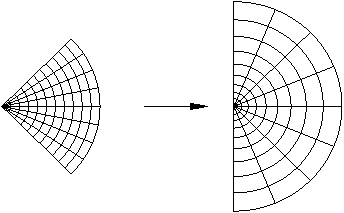
\includegraphics{figures/zsqplot}
\caption{What $z^2$ does to the sector
$\frac{-\pi}{2} \leq \operatorname{Arg} z \leq \frac{\pi}{2}$, $\sabs{z} <
1.1$.\label{fig:zsqplot}}
\end{myfig}

\begin{exbox}
\begin{exercise}
Prove that
\begin{exparts}
\item
If $\sabs{z}<1$, then $\lim\limits_{n\to \infty} z^n = 0$.
\item
If $\sabs{z}>1$, then $\lim\limits_{n\to \infty} z^n = \infty$.
\item
If $z \not= 1$ is such that $\sabs{z}=1$, then $z^n$ diverges as $n \to
\infty$.
\end{exparts}
\end{exercise}

\begin{exercise}[Easy]
On the unit circle parametrized by the angle $\theta$,
write $\sin(n\theta)$ and $\cos(n\theta)$ as a linear combination
of powers (including negative) of $z = e^{i\theta}$.
\end{exercise}
\end{exbox}

\subsection{Power series and radius of convergence}

A \emph{\myindex{power series}} around $p \in \C$ is simply the series
\glsadd{not:powerser}%
\begin{equation*}
\sum_{n=0}^\infty c_n {(z-p)}^n ,
\end{equation*}
where $c_n$ are some complex numbers.  Where it converges it defines a
function of $z$.  As the series clearly converges at $z=p$, we worry about
convergence at other points.  We say the series is
\emph{convergent}\index{convergent power series}, if there is
some $z \not= p$ where the series converges.

The most important series, and in some sense the only one that we really
know how to sum, is the \emph{\myindex{geometric series}}.

\begin{prop}[Geometric series]\label{prop:geomseries}
\leavevmode
\begin{enumerate}[(i)]
\item For $z \in \D$,
\begin{equation*}
\frac{1}{1-z} = \sum_{n=0}^\infty z^n .
\end{equation*}
\item For $z \not\in \D$,
\begin{equation*}
\sum_{n=0}^\infty z^n \quad \text{diverges.}
\end{equation*}
\item
Given $0 < r < 1$, then for all $z \in \overline{\Delta_r(0)}$
(that is, $\sabs{z} \leq r$)
\begin{equation*}
\abs{\frac{1}{1-z} - \sum_{n=0}^m z^n}
\leq \frac{r^{m+1}}{1-r} .
\end{equation*}
Consequently,
as $\frac{r^{m+1}}{1-r} \to 0$,
the geometric series converges uniformly
on $\overline{\Delta_r(0)}$.
\end{enumerate}
\end{prop}

\begin{proof}
All three items follow (details left as exercise) from
\begin{equation*}
1+z+z^2+\cdots+z^m = \frac{1-z^{m+1}}{1-z} ,
\end{equation*}
for all $z \not= 1$, which follows by expanding 
$(1-z)(1+z+z^2+\cdots+z^m)$.
\end{proof}

\begin{exbox}
\begin{exercise}
Fill in the details of the proof of \propref{prop:geomseries}.  Do not forget
about the boundary of the disc.
\end{exercise}
\end{exbox}

A power series converges absolutely if the following series converges:
\begin{equation*}
\sum_{n=0}^\infty \sabs{c_n} \sabs{z-p}^n .
\end{equation*}
For $N < M$,
\begin{equation*}
\abs{\sum_{n=N+1}^M c_n {(z-p)}^n}
\leq
\sum_{n=N+1}^M \sabs{c_n} \sabs{z-p}^n.
\end{equation*}
Hence, if the sequence of partial sums of 
$\sum \sabs{c_n} \sabs{z-p}^n$ is Cauchy, so is the sequence
of partial sums of $\sum c_n {(z-p)}^n$.  Thus,
an absolutely convergent series
actually converges.

Let $r = \sabs{z-p}$, then we have the real series $\sum \sabs{c_n} r^n$.  Define
\begin{equation} \label{eq:rconvdef}
R = \frac{1}{\limsup\limits_{n \to \infty} \sqrt[n]{\sabs{c_n}}} ,
\end{equation}
where we interpret $\nicefrac{1}{\infty} = 0$ and $\nicefrac{1}{0} = \infty$,
so $R=\infty$ is allowed.\footnote{%
This is not the \myquote{extended reals sense,}
we are really extending just the nonnegative reals, and that's why
something like $\nicefrac{1}{0}=\infty$ makes sense here, for the same
reason as on the Riemann sphere.}
By the standard root test, the series $\sum \sabs{c_n} r^n$
converges if
\begin{equation*}
\limsup_{n \to \infty} \sqrt[n]{\sabs{c_n} r^n} = 
r \limsup_{n \to \infty} \sqrt[n]{\sabs{c_n}} = r \frac{1}{R} < 1 ,
\end{equation*}
and it diverges if $r \frac{1}{R} > 1$.  In other words,
the series converges if
$r < R$
and diverges if
$r > R$.  See \figureref{fig:radiusconvcomplex}.
We have proved the following proposition:

\begin{prop}[Cauchy--Hadamard theorem\footnote{%
Cauchy published this result in 1821, and Hadamard, despite also being
French, didn't know about it and published it in his thesis in 1888.}]
\index{Cauchy--Hadamard theorem}
A power series $\sum c_n {(z-p)}^n$ converges absolutely if
$\sabs{z-p} < R$ and diverges if
$\sabs{z-p} > R$, where $R$ is defined by \eqref{eq:rconvdef}.
\end{prop}

\begin{myfig}
\subimport*{figures/}{radiusconvcomplex.pdf_t}
\caption{Radius of convergence.\label{fig:radiusconvcomplex}}
\end{myfig}

The number $R$ is called the \emph{\myindex{radius of convergence}}.
The power series converges absolutely
in the disc $\Delta_R(p)$, and diverges
in the complement of the closure $\overline{\Delta_R(p)}$.
Convergence (or divergence) on the boundary circle $\partial \Delta_R(p)$
is a tricky matter.

A useful criterion for convergence is that the sequence
$\bigl\{ \sabs{c_n} r^n \bigr\}$ is
bounded whenever $0 < r < R$.

\begin{prop} \label{prop:cnrnbounded}
The series $\sum c_n {(z-p)}^n$ converges in $\Delta_{R}(p)$ for some
$R > 0$ if and only if
for every $r$ with
$0 < r < R$ there exists an $M > 0$ such that
\begin{equation*}
\sabs{c_n} \leq \frac{M}{r^n} \qquad \text{for all } n .
\end{equation*}
\end{prop}

It is not necessarily true that $\bigl\{ \sabs{c_n} R^n \bigr\}$
is bounded if $R$ is the radius of convergence.
The series $\sum z^n$ and $\sum n z^n$ have
radius of convergence 1, while the sequence of coefficients
is bounded in the first case and
not in the second.  However, $\{ n r^n \}$ is bounded for all $r < 1$.

\begin{proof}
Suppose the series converges in $\Delta_{R}(p)$ and
$0 < r < R$, then $\sum \sabs{c_n}r^n$ converges,
and the terms of that series are bounded.

Conversely, fix $r$, suppose 
$\sabs{c_n} r^n \leq M$ for all $n$, and suppose $0 < s < r$.
Then
\begin{equation*}
\sqrt[n]{\sabs{c_n} s^n}=
\frac{s}{r}\sqrt[n]{\sabs{c_n} r^n} \leq \frac{s}{r} \sqrt[n]{M} .
\end{equation*}
The limsup of the right-hand side is strictly less than 1 as $\nicefrac{s}{r} < 1$.
So the series converges absolutely in
$\overline{\Delta_s(p)}$.  As $s$ and $r$ with $0 < s < r < R$ were
arbitrary,
the series converges (absolutely) in $\Delta_R(p)$.
\end{proof}

The proof is farily typical for convergence results of power series.
Convergence in $\Delta_R(p)$, means boundedness of
$\{ \sabs{c_n} r^n \}$ in a smaller $\Delta_r(p)$, which only gets us convergence
in $\Delta_s(p)$.  See \figureref{fig:threediscs}.  But since $s$ and $r$
are arbitrary we get convergence everywhere.
\begin{myfig}
\subimport*{figures/}{threediscs.pdf_t}
\caption{The three discs from the convergence proof.\label{fig:threediscs}}
\end{myfig}

\begin{exbox}
\begin{exercise}
Prove the triangle inequality for series.  If $\sum_{n=0}^\infty c_n$
converges, then $\abs{\sum_{n=0}^\infty c_n} \leq \sum_{n=0}^\infty
\sabs{c_n}$ (the right-hand side is possibly $\infty$).
\end{exercise}
\end{exbox}

The convergence inside the radius of convergence is even nicer than just absolute.
Let $K \subset \C$ be a set.
A power series $\sum c_n {(z-p)}^n$
\emph{\myindex{converges uniformly absolutely}}\index{uniform absolute convergence}
for $z \in K$ when $\sum \sabs{c_n} \sabs{z-p}^n$
converges uniformly for $z \in K$.
Suppose a series converges uniformly absolutely.  It converges absolutely,
so it converges, and 
\begin{equation*}
\abs{
\sum_{n=0}^\infty c_n {(z-p)}^n
-
\sum_{n=0}^{m} c_n {(z-p)}^n
}
=
\abs{\sum_{n=m+1}^\infty c_n {(z-p)}^n} \leq
\sum_{n=m+1}^\infty \sabs{c_n} \sabs{z-p}^n .
\end{equation*}
The right-hand side goes to zero uniformly in $z \in K$,
and so
a uniformly absolutely convergent series also converges
uniformly.  So the name fits the crime.

\begin{prop}
Let $\sum c_n {(z-p)}^n$ be a power series with radius of convergence $R
> 0$.  If $0 < r < R$, then the power series converges uniformly absolutely
in $\overline{\Delta_r(p)}$. Furthermore, let $U = \Delta_R(p)$ if $R < \infty$ and
$U = \C$ if $R=\infty$, and let $K \subset U$ be compact.
Then the series converges uniformly absolutely on $K$.
\end{prop}

Less formally, power series converges uniformly (absolutely) on
compact subsets of its domain of convergence.

\begin{proof}
Without loss of generality suppose $R < \infty$.
Suppose $0 < r < R$.  As $\sum c_n {(z-p)}^n$ converges absolutely
on $\Delta_R(p)$, the series
$\sum \sabs{c_n} r^n$ converges (and in particular any tail of
that series converges).  Thus for $z \in \overline{\Delta_r(p)}$,
\begin{equation*}
\abs{
\sum_{n=0}^\infty \sabs{c_n} \sabs{z-p}^n
-
\sum_{n=0}^{m} \sabs{c_n} \sabs{z-p}^n
}
\leq
\sum_{n=m+1}^\infty \sabs{c_n} r^n .
\end{equation*}
The right-hand side, which does not depend on $z$,
goes to zero as $m \to \infty$, and hence 
the series $\sum \sabs{c_n} \sabs{z-p}^n$ converges uniformly in $\overline{\Delta_r(p)}$.

If $K \subset \Delta_{R}(p)$ is compact, then there exists some $r <
R$ such that $K \subset \Delta_r(p)$ (consider an open cover of
$K$ by discs $\Delta_r(p)$ for all $r < R$).  The result follows.
\end{proof}

\begin{exbox}
\begin{exercise}
Show that the series $\sum_{n=1}^\infty \frac{1}{n^2} z^{n}$ has radius of
convergence $1$, and
show that it converges absolutely on the boundary of the unit disc.  Hence
it actually converges uniformly on the entire closed unit disc.
\end{exercise}

\begin{exercise}
Show that
$\sum_{n=0}^\infty n^n z^{n^n}$ has radius of convergence $1$,
while
$\sum_{n=0}^\infty n^n z^{n}$ is not convergent at all.
\end{exercise}

\begin{exercise}
Suppose
$\sum_{n=0}^\infty c_n z^{n}$ converges at $z=1$, but not absolutely.
Prove that the radius of convergence is 1.
\end{exercise}

\begin{exercise}[Weierstrass $M$-test]
\label{exercise:weierMtest}
Let $X$ be a set and suppose that $f_n \colon X \to \C$ is
a sequence of functions such that
$\abs{f_n(x)} \leq M_n$ for all $x \in X$ and $n \in \N$.  If $\sum M_n <
\infty$, then $\sum f_n(x)$ converges uniformly absolutely on $X$
($\sum \sabs{f_n(x)}$ converges uniformly on $X$).
\end{exercise}

\begin{exercise}
Suppose
$\sum_{n=0}^\infty a_n z^{n}$ and $\sum_{n=0}^\infty b_n z^{n}$
have a radius of convergence at least $r > 0$.  Show that
the sum series
$\sum_{n=0}^\infty (a_n+b_n) z^{n}$ has a radius of convergence at least
$r$ and converges to the sum of the two series.
\end{exercise}

\begin{exercise}
Given an $R > 1$, find two power series
$\sum_{n=0}^\infty a_n z^{n}$ and $\sum_{n=0}^\infty b_n z^{n}$,
such that both have radius of convergence exactly 1, but the 
sum
$\sum_{n=0}^\infty (a_n+b_n) z^{n}$ has a radius of convergence 
exactly $R$.  Hint: First figure out a series with radius of convergence
exactly $R$.
\end{exercise}

\begin{exercise}
Suppose
$\sum_{n=0}^\infty a_n z^{n}$ and $\sum_{n=0}^\infty b_n z^{n}$
have a radius of convergence at least $r > 0$.  Let 
$c_n = \sum_{k=0}^n a_{n-k}b_k$.  Show that
the series
$\sum_{n=0}^\infty c_n z^{n}$ has a radius of convergence at least
$r$ and converges to the product of the two series.
Hint: The key is to look at a point where both series converge absolutely,
then use the absolute convergence.
\end{exercise}
\end{exbox}

\begin{remark}
The last few exercises say that we can add and multiply series; however,
we won't really need them as the two results are easy for holomorphic
functions, and we will show later that power series are
holomorphic and vice versa.  You should still try them, they are good
practice.
\end{remark}

%%%%%%%%%%%%%%%%%%%%%%%%%%%%%%%%%%%%%%%%%%%%%%%%%%%%%%%%%%%%%%%%%%%%%%%%%%%%%%

\section{Analytic functions}
\label{sec:analfuncs}

\subsection{Definition}

Functions that possess a convergent power series are called analytic.
From the beginnings of calculus until the 19\textsuperscript{th} century, 
when mathematicians considered a \myquote{function} they really meant
\myquote{analytic function} (or something like it) in modern language.
One can talk about
both complex-analytic and real-analytic functions depending on if the
variables are real or complex, and they may depend on one or several variables,
but we are interested in complex-analytic functions of one variable. 
As there is little chance of confusion, we say just \myquote{analytic} instead of
\myquote{complex-analytic.}

\begin{defn}
Let $U \subset \C$ be open.  A function $f \colon U \to \C$
is \emph{\myindex{analytic}}\index{complex-analytic}
if for every $p \in U$, there exists 
an $r > 0$ and a
power series $\sum c_n {(z-p)}^n$ converging to $f$ on $\Delta_r(p) \subset
U \subset \C$.
\end{defn}

\begin{exbox}
\begin{exercise}[Easy]
Prove that polynomials $P(z)$ are analytic.
\end{exercise}

\begin{exercise}
Prove that $\nicefrac{1}{z}$ is analytic in $\C \setminus \{ 0 \}$
by explicitly writing down 
a power series at any $p \in \C \setminus \{ 0 \}$
using the geometric series.
\end{exercise}

\begin{exercise}
Suppose $f(z) = \sum_{n=0}^\infty a_n z^n$ converges and defines a
function on $\D$ such that $f(z) = f(-z)$ for all $z \in \D$ ($f$ is
\myquote{even}).
Prove that there exists a function defined by a power series
$g(z) = \sum_{n=0}^\infty b_n z^n$ converging in $\D$ such that
$f(z) = g(z^2)$.
\end{exercise}
\end{exbox}

\subsection{Analytic functions are holomorphic}

Eventually, we will see that analytic functions and holomorphic functions are
one and the same.\footnote{%
For this reason, some authors define \myquote{analytic} to mean complex differentiable,
which is no problem eventually, but right now it would be.}
We start by proving that
analytic functions are holomorphic, that is, they are complex
differentiable.

\begin{prop}
\pagebreak[2]
Let $f \colon \Delta_R(p) \to \C$ be defined by
\begin{equation*}
f(z) = \sum_{n=0}^\infty c_n {(z-p)}^n ,
\qquad \text{converging in } \Delta_R(p) .
\end{equation*}
Then $f$ is complex differentiable at every $z \in \Delta_R(p)$ and
\begin{equation*}
f'(z) = \sum_{n=1}^\infty n c_n {(z-p)}^{n-1} ,
\qquad \text{converging in } \Delta_R(p) .
\end{equation*}
\end{prop}

\begin{proof}
Without loss of generality, let $p=0$.
Differentiate $z^n$ at $z_0$ by considering the difference
quotient
\begin{equation*}
\frac{z^n-z_0^n}{z-z_0}
=
\sum_{k=0}^{n-1}
z^k z_0^{n-1-k} ,
\end{equation*}
which goes to $n z_0^{n-1}$ as $z \to z_0$.
Apply the formula to $f$
term-wise.  For $z_0,z \in \Delta_R(0)$,
\begin{equation*}
\frac{f(z) - f(z_0)}{z-z_0}
=
\sum_{n=1}^\infty c_n \frac{z^n-z_0^n}{z-z_0}
=
\sum_{n=1}^\infty c_n \sum_{k=0}^{n-1} z^k z_0^{n-1-k} .
\end{equation*}
The right-hand side is defined even if $z_0 = z$.
We must show that this expression is continuous as a function of $z$
at $z_0$.
It is continuous provided that the series
in the expression converges uniformly for $z$ in a
neighborhood of $z_0$.

The setup will be just like in \figureref{fig:threediscs}.
Let $r$ and $s$ be such that $0 < s < r < R$ and suppose that $z_0$ and $z$ are
in $\Delta_s(0)$.
\begin{equation*}
\abs{c_n \sum_{k=0}^{n-1} z^k z_0^{n-1-k}}
\leq
\sum_{k=0}^{n-1} 
\sabs{c_n} s^{n-1}
=
n
\sabs{c_n} s^{n-1}
=
n
\sabs{c_n} r^{n-1} {\left(\frac{s}{r}\right)}^{n-1} .
\end{equation*}
The expression
$\sabs{c_n} r^{n-1}$ is bounded by some $M > 0$ because the series for $f$ converges
in $\Delta_R(0)$ and $r < R$.
As
\begin{equation*}
\sqrt[n]{
n \sabs{c_n} s^{n-1}
}
=
\sqrt[n]{
n \sabs{c_n} r^{n-1} {\left(\frac{s}{r}\right)}^{n-1}
}
\leq
\sqrt[n]{
n M {\left(\frac{s}{r}\right)}^{n-1}
}
\quad\underset{\text{as } n \to \infty}{\to}\quad
\frac{s}{r} < 1 ,
\end{equation*}
the root test shows that
$\sum n \sabs{c_n} s^{n-1}$
converges.
So the series for the difference quotient,
\begin{equation*}
\sum_{n=1}^\infty c_n \sum_{k=0}^{n-1} z^k z_0^{n-1-k} ,
\end{equation*}
converges uniformly in $z$ on $\Delta_s(p)$, and
we can swap the limit $z \to z_0$ with the series limit:
\begin{equation*}
\lim_{z \to z_0}
\frac{f(z)-f(z_0)}{z-z_0}
=
\sum_{n=1}^\infty c_n \sum_{k=0}^{n-1} z_0^k z_0^{n-1-k}
=
\sum_{n=1}^\infty n c_n z_0^{n-1} .
\end{equation*}
As $s$ and $r$ were arbitrary, the convergence happens in all of
$\Delta_R(0)$.
\end{proof}

So the derivative of a power series is again given by a power series.
By induction, it follows that a power series is infinitely complex
differentiable.

\begin{cor} \label{cor:convpowserinfdif}
\pagebreak[2]
Let $f \colon \Delta_R(p) \to \C$ be defined by a convergent power series
\begin{equation*}
f(z) = \sum_{n=0}^\infty c_n {(z-p)}^n .
\end{equation*}
Then $f$ is infinitely complex differentiable in $\Delta_R(p)$,
and the $k$\textsuperscript{th} derivative is given by
\begin{equation*}
f^{(k)}(z) = \sum_{n=k}^\infty n(n-1)\cdots(n-k+1) c_n {(z-p)}^{n-k} ,
\qquad \text{converging in } \Delta_R(p) .
\end{equation*}
Furthermore,
\begin{equation*}
c_n =
\frac{f^{(n)}(p)}{n!} .
\end{equation*}
\end{cor}

\begin{exbox}
\begin{exercise}
Fill in the details of the proof of the corollary.
\end{exercise}
\end{exbox}

An important consequence of this corollary that should be
emphasized is that if $f$ is given by the convergent power series in
$\Delta_R(p)$ as above, then the power series is unique.  This conclusion
follows from the formula for the coefficients $c_n$.  In fact, the
coefficients depend only on the values of $f$ in an arbitrarily small
neighborhood of $p$.

If we apply the corollary to analytic functions at every point,
we find that they are infinitely differentiable:

\begin{cor} \label{cor:analinfdif}
An analytic function is infinitely complex differentiable, and each
derivative is analytic.
\end{cor}

\begin{remark}
A subtle issue is that while we proved that analytic functions are
complex differentiable because they have a power series representation,
we did not yet prove that a convergent power series defines an analytic
function.  What is left is to prove that a power series convergent
in $\Delta_R(p)$ can be
expanded about a different point in $\Delta_R(p)$.  That will follow
once we prove that holomorphic functions are analytic.
\end{remark}

\begin{exbox}
\begin{exercise}
Suppose $f \colon \Delta_R(0) \to \C$ is given by a convergent power
series
$f(z) = \sum_{n=0}^\infty c_n z^n$.
Suppose that for some $\epsilon > 0$, $f(x) = 0$ for all $x \in
(-\epsilon,\epsilon)$ (an interval on the real line).
Using the corollary,
prove that $c_n = 0$ for all $n$ and hence $f$ is identically zero.
\end{exercise}

\begin{exercise} \label{exercise:antidefpowerser}
Suppose $f \colon \Delta_R(p) \to \C$ is given by a convergent power
series
$f(z) = \sum_{n=0}^\infty c_n {(z-p)}^n$.
Antidifferentiate:
Show that there exists a power series converging in $\Delta_R(p)$
whose complex derivative is $f(z)$.
\end{exercise}

\begin{exercise} 
Suppose $f \colon \Delta_R(0) \to \C$ is given by a convergent power
series
$f(z) = \sum_{n=0}^\infty c_n {z}^n$ and $R > 1$.
Show that there is an $M>0$ such that
$\sabs{f^{(n)}(0)} \leq n! M$ for all $n$.
\end{exercise}
\end{exbox}

\subsection{The exponential}

We met the complex exponential $e^z$ before
(\subsectionref{subsection:firstdefexp}), and we proved
that it is holomorphic and its own derivative
(\exerciseref{exercise:exponentialholomorphic}).  We can now see this fact
from a different vantage point.\footnote{%
That vantage point being the same as that dark place in your past
that is the undergraduate differential equations class when you covered
power series methods for solving ODEs.}
We claim we could have defined the exponential
using a power series.

\begin{prop}
The power series
\begin{equation*}
f(z) = \sum_{n=0}^\infty \frac{1}{n!} z^n ,
\end{equation*}
is the unique convergent power series at the origin
such that $f(0)=1$ and $f'=f$.
Moreover, the series converges on $\C$ and
$f(z) = e^z$.
\end{prop}

\begin{proof}
It is not hard to check directly (exercise)
that the series converges in all of $\C$.
We now know that power series are holomorphic and we know how
to differentiate them, we do it term-by-term, that is, \myquote{formally.}
Let $f$ be a convergent power series at the origin
\begin{equation*}
f(z) = \sum_{n=0}^\infty c_n z^n ,
\end{equation*}
such that $f(0)=1$ and $f'=f$.
Obviously, $f(0)=1$ implies that $c_0 = 1$.
The trick is to figure out the rest of the series.
So,
\begin{equation*}
f'(z) =
\sum_{n=1}^\infty n c_n z^{n-1} =
\sum_{n=0}^\infty (n+1) c_{n+1} z^{n} .
\end{equation*}
As the coefficients of the power series at zero are unique, we get
$c_n = (n+1) c_{n+1}$.  By induction, $c_n = \frac{1}{n!}$.

Let us prove that $f$ is the exponential.  Both functions are
holomorphic, the exponential is never zero, and both are equal to their
derivatives.  So,
\begin{equation*}
\frac{d}{dz} \left[ \frac{f(z)}{\exp(z)} \right]
=
\frac{f'(z)\exp(z) - f(z) \exp'(z)}{{\bigl(\exp(z)\bigr)}^2}
=
\frac{f(z)\exp(z) - f(z) \exp(z)}{{\bigl(\exp(z)\bigr)}^2}
= 0.
\end{equation*}
Hence, $f(z) = C \exp(z)$ for some constant (\propref{prop:zeroder}).
As $f(0) = \exp(0) = 1$,
we conclude $C=1$.
\end{proof}

\begin{exbox}
\begin{exercise}
Prove that the series for the exponential converges by computing
the radius of convergence directly
(e.g., show that the series converges for every $z \in \C$).
\end{exercise}

\begin{exercise}
Compute the series for $\sin z$ and $\cos z$, then show that these satisfy
$f''(z) = -f(z)$.
\end{exercise}

\begin{exercise}
Show that there exists a holomorphic $f \colon \C \to \C$ that
solves $f'(z) + z f(z) = 0$ and such that $f(0) = 1$.  Hint: Solve formally
as a power series,
then see if you can guess the answer in \myquote{closed form,} that is, in terms
of the exponential.  Hint \#2: What is $f'(0)$?
\end{exercise}

\begin{exercise}
Given $a,b \in \C$, show that there exists a holomorphic $f \colon \C \to
\C$ such that $f''(z) = z f(z)$, and $f(0) = a$ and $f'(0) = b$.
Hint: Define formally and show convergence.
Note: These are the \emph{\myindex{Airy functions}}, and they have some
interesting behavior; on the real line they oscillate like sine and cosine
for negative $z$ and behave like an exponential for positive $z$.
\end{exercise}
\end{exbox}

\subsection{The identity theorem}

One of the main properties of analytic functions is that once you know them
in a neighborhood you know them everywhere.  In fact, a much more general
statement is true; you only need to know an analytic function on a set with
a limit point.

\begin{thm}[Identity]\index{identity theorem!holomorphic functions}%
\label{thm:identity}
Suppose $U \subset \C$ is a domain, 
and $f \colon U \to \C$ analytic.
If $Z_f = \bigl\{ z \in U : f(z) = 0 \bigr\}$
has a limit point in $U$, then $f$ is identically zero.
In other words, all points of $Z_f$ are isolated unless $f \equiv 0$.
\end{thm}

\begin{defn}
The points in the set $Z_f$ are called the \emph{zeros}\index{zero} of $f$.
\end{defn}

The \myquote{In other words} bit is
one consequence of this theorem that we will use very often.  More
concretely, if $f(p)=0$, but $f$ is not
identically zero, then there is a disc $\Delta_r(p)$ such that $f(z) \not=
0$ for all $z \in \Delta_r(p) \setminus \{ 0 \}$.

Another common application of the theorem is the following weaker statement:
\myquote{If the function is zero on a nonempty open subset, then $f \equiv 0$.}
Think of the implications:  If $f \colon U \to \C$ is analytic, and we know
$f$ in a tiny disc $\Delta_r(p)$ for an arbitrarily small $r$, then
we know $f$ on all of $U$.

\begin{proof}
Suppose $f$ is not identically zero.
The set $Z_f$ is closed as $f$ is continuous.  So we have to show
that points of $Z_f$ are isolated.
Without loss of generality suppose that $0 \in U$ and $0 \in Z_f$,
and suppose $0$ is not in the interior of $Z_f$.
Write $f$ near $0$ as
\begin{equation*}
f(z) = \sum_{n=0}^\infty c_n z^n .
\end{equation*}
As $f(0) = 0$, $c_0 =0$.  Let $k$ be the first $k$ such that $c_k \not=0$,
such a $k$ exists as otherwise $f$ would be identically zero near $0$
and we assumed $0$ is not in the interior of $Z_f$.  Then
\begin{equation*}
f(z) = z^k \sum_{n=k}^\infty c_n z^{n-k} = z^k g(z) .
\end{equation*}
The series $g(z)$ is a convergent power series and $g(0) = c_k \not=
0$.  A power series is continuous, and hence $g(z) \not= 0$ in a whole
neighborhood of $0$.
As $z^k$ is only zero at $0$, we find that $0$ is an isolated zero of $f$.

So the only points of $Z_f$ that are not isolated are those that are in the
interior of $Z_f$.  Let $Z_f' \subset Z_f$ be the set of nonisolated points
of $Z_f$.  This set must be closed as $Z_f$ is closed, and no sequence
of points in $Z_f'$ can
have an isolated point of $Z_f$ as a limit.
We have proved above that nonisolated
points must be interior points of $Z_f$ (and hence of $Z_f'$).
So $Z_f'$ is both open and closed.  As $U$ is connected and 
that $Z_f' \not= U$, we conclude $Z_f' = \emptyset$.
Thus all points of $Z_f$ are isolated.
\end{proof}

\begin{exbox}
\begin{exercise}
Suppose $U \subset \C$ is a domain,
$f \colon U \to \C$ and $g \colon U \to \C$ are analytic,
and the set $\bigl\{ z \in U : f(z) = g(z) \bigr\}$ has a limit
point in $U$.
Prove that $f \equiv g$.
\end{exercise}

\begin{exercise}
\begin{exparts}
\item
Suppose $U \subset \C$ is a domain,
$f \colon U \to \C$ and $g \colon U \to \C$ are analytic,
and $f(z)g(z) = 0$ for all $z \in U$.
Prove that either $f$ or $g$ is identically zero.
(In other words, the ring of holomorphic functions on $U$ is an integral
domain.)
\item
Find an open but disconnected $U$ and holomorphic $f$ and $g$,
such that still $fg = 0$, but neither $f$ nor $g$ is identically zero.
\end{exparts}
\end{exercise}

\begin{exercise}
Suppose $U \subset \C$ is a domain and $f \colon U \to \C$ is
analytic and not constant.  Show that if $K \subset U$ is compact,
then $Z_f \cap K$ is finite.
\end{exercise}

\begin{exercise}
Suppose $U \subset \C$ is a domain, $f \colon U \to \C$ and $g \colon U \to
\C$ are analytic, and $p \in U$.  Suppose that $f^{(k)}(p) = g^{(k)}(p)$
for $k=0,1,2,\ldots$.  Prove that $f \equiv g$.
\end{exercise}

\begin{exercise}
Suppose $U \subset \C$ is a domain and $f \colon U \to \C$ is analytic.
Prove that if $f'(z) = 0$ for
all $z$ in a neighborhood of some $z_0 \in U$, then $f$ is constant.
\end{exercise}

\begin{exercise}
Suppose $U \subset \C$ is a domain, $a, b, c \in \C$, and $z_0 \in U$.
Show that
an analytic solution $f$ on $U$ to the linear equation $f'(z) = a f(z) + b$
given $f(z_0) = c$ is unique.  Hint: Show that the power series at $z_0$ is uniquely
determined.
\end{exercise}
\end{exbox}

One of the downsides of analytic functions is that there are no compactly
supported analytic functions on $\C$.  The \emph{\myindex{support}}
of a function $f \colon U
\to \C$ is the closure (in $U$) of the set
$\bigl\{ z \in U : f(z) \not= 0 \bigr\}$, that is, 
the support is $\overline{U \setminus Z_f} \cap U$.

\begin{exbox}
\begin{exercise}
Let $U \subset \C$ be a domain and $f \colon U \to \C$ is analytic and
is not identically zero.
Show that the support of $f$ is $U$.
In particular, the support cannot be compact.
\end{exercise}
\end{exbox}



%%%%%%%%%%%%%%%%%%%%%%%%%%%%%%%%%%%%%%%%%%%%%%%%%%%%%%%%%%%%%%%%%%%%%%%%%%%%%%
%%%%%%%%%%%%%%%%%%%%%%%%%%%%%%%%%%%%%%%%%%%%%%%%%%%%%%%%%%%%%%%%%%%%%%%%%%%%%%
%%%%%%%%%%%%%%%%%%%%%%%%%%%%%%%%%%%%%%%%%%%%%%%%%%%%%%%%%%%%%%%%%%%%%%%%%%%%%%

\chapter{Line Integrals and Rudimentary Cauchy Theorems} \label{ch:cauchysimple}

\begin{myepigraph}
The Brain: Pinky, are you pondering what I am pondering?

Pinky:  Uh, I think so, Brain, but we'll never get a monkey to use dental floss.
\end{myepigraph}

%%%%%%%%%%%%%%%%%%%%%%%%%%%%%%%%%%%%%%%%%%%%%%%%%%%%%%%%%%%%%%%%%%%%%%%%%%%%%%

\section{Line integrals}
\label{sec:lineints}

\subsection{Paths}

\begin{defn}
\glsadd{not:contdifffuncs}%
A \emph{\myindex{piecewise-$C^1$ path}} or a \emph{\myindex{path}} for short
is
a continuous complex-valued piecewise continuously
differentiable function $\gamma \colon [a,b] \to \C$ 
such that $\gamma'(t)$ and all its one-sided limits are never
0.\footnote{Some authors do not require the derivative not being zero, and
in fact in the way that we use the paths, the requirement is not crucial,
but leaving it off does lead to allowing some strange paths.}
A path $\gamma$ is \emph{closed}\index{closed path} if $\gamma(a)=\gamma(b)$.
A path $\gamma$ is \emph{simple closed}\index{simple closed path}
if $\gamma(a)=\gamma(b)$ and $\gamma|_{(a,b]}$ is injective.
\end{defn}

Our paths will essentially all be piecewise-$C^1$,
so we may forget to mention it sometime.
By \myquote{piecewise-$C^1$,}
we mean that there exist numbers $t_0 = a < t_1 < \cdots
< t_k = b$ for some $k$ such that $\gamma|_{[t_{\ell-1},t_\ell]}$ is
continuously differentiable ($C^1$) up to
the boundary for every $\ell$ and its derivative is never zero.
In other words, $\gamma$ is continuously differentiable inside all the
subintervals $(t_{\ell-1},t_\ell)$, $\gamma'$ is never zero, the one-sided limits
\begin{equation*}
\lim_{t \uparrow t_\ell} \gamma'(t) \qquad
\lim_{t \downarrow t_\ell} \gamma'(t)
\end{equation*}
exist for all $\ell$ (except, of course, only one exists at $a$ or $b$),
and these limits are nonzero.
Another way to say it is that $\gamma'(t)$ extends to a nonzero
continuous function on each closed interval $[t_{\ell-1},t_{\ell}]$.
Allowing these \myquote{corners} makes working with paths easier
as we can define them easily piece-wise, and finitely many corners like
this make no difference for integrals.
Do note also that we are saying that paths are continuous.  We will allow
discontinuities just a little later with \myquote{chains.}

When we say that $\gamma$ is a path in $U \subset \C$\index{path in $U$},
we mean that
$\gamma \colon [a,b] \to U$ is a path.  Another common abuse of notation we
will freely and shamelessly commit is that if we refer to $\gamma$
as if it were a set we mean the image $\gamma\bigl([a,b]\bigr)$.
Nowhere will we really use or need that $\gamma'$ is never zero,
but leaving that off would allow some paths that one would generally not
wish to call piecewise-$C^1$,
as you will see in the exercises.

\begin{example} \label{example:squarepath}
The path $\gamma \colon [0,4] \to \C$, given by
\begin{equation*}
\gamma(t) =
\begin{cases}
t          & \text{if } t \in [0,1],\\
1 + i(t-1) & \text{if } t \in (1,2],\\
3-t + i    & \text{if } t \in (2,3],\\
i(4-t)     & \text{if } t \in (3,4],
\end{cases}
\end{equation*}
is a piecewise-$C^1$ path traversing the sides unit square.
See \figureref{fig:squarepath}.  You should check that the
conditions are satisfied.  For example, 
on $t \in (0,1)$, $\gamma'(t) = 1$, and so
$\lim_{t \uparrow 1} \gamma'(t) = 1$.  Similarly
$\lim_{t \downarrow 1} \gamma'(t) = i$, and so on.
\begin{myfig}
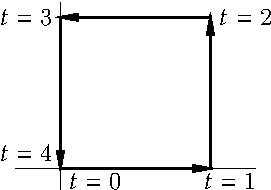
\includegraphics{figures/squarepath}
\caption{The path $\gamma$ traversing the unit square.\label{fig:squarepath}}
\end{myfig}
\end{example}

\subsection{The line integral}

\begin{defn}
Given a piecewise-$C^1$ path $\gamma \colon [a,b] \to \C$ and a continuous
function $f$ on 
$\gamma$, 
we define the \emph{\myindex{line integral}}\footnote{%
This integral is also called
a \emph{\myindex{path integral}}, 
a \emph{\myindex{curve integral}}, or
a \emph{\myindex{contour integral}}.}
\glsadd{not:pathint}%
\begin{equation*}
\int_{\gamma} f(z) \, dz
\overset{\text{def}}{=}
\int_a^b f\bigl(\gamma(t)\bigr) \gamma'(t) \, dt .
\end{equation*}
\end{defn}

The right hand side makes sense.
The integrand is undefined
at finitely many points (where $\gamma'(t)$ does not exist),
but it is piecewise continuous, and this is enough
to be Riemann integrable: On each closed interval
$[t_{\ell-1},t_\ell]$, the integrand extends to a continuous
function.
Note that the definition makes sense even if $\gamma'(t)$ is zero somewhere.

Let us compute the most important example of a line integral.

\begin{example} \label{example:integralpowerz}
Let $\gamma \colon [0,2\pi] \to \C$ given by $\gamma(t) = r e^{it}$ be
the circle of radius $r$ oriented counterclockwise,
that is, $\partial \Delta_r(0)$.  See \figureref{fig:circlepath}.
For $n \in \Z$, we claim that
\begin{equation*}
\int_\gamma z^n \, dz
=
\begin{cases}
2\pi i & \text{if } n=-1, \\
0 & \text{otherwise.}
\end{cases}
\end{equation*}

\begin{myfig}
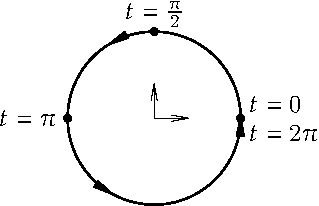
\includegraphics{figures/circlepath}
\caption{The path $\gamma$ traversing the circle.\label{fig:circlepath}}
\end{myfig}

First, $\gamma'(t) = i r e^{it}$.
To prove the claim we compute
\begin{equation*}
\int_\gamma z^n \, dz
=
\int_0^{2\pi}
r^n
e^{int} i r e^{it} \, dt
=
i r^{n+1}
\int_0^{2\pi}
e^{i(n+1)t} \, dt .
\end{equation*}
The result follows as the integral on the right-hand side is zero
(write it in terms of sines and cosines, exercise below), unless $n+1 = 0$,
in which case, the integral 
is $2\pi$ and $r^{n+1} = 1$.  Note in particular that the value of the
integral does not depend on $r$.
\end{example}

\begin{exbox}
\begin{exercise}
Prove that if $k\not= 0$, then $\int_0^{2\pi} e^{ik t} \, dt = 0$.
\end{exercise}

\begin{exercise}
Let $f(z) = \sum_{n=-d}^d c_n z^n$ and $\gamma$ as in
\exampleref{example:integralpowerz}.
Compute $\int_\gamma f(z) \, dz$.
\end{exercise}

\begin{exercise}
Compute $\int_\gamma \bar{z}^n \, dz$ for all $n \in \Z$ and $\gamma$ as in
\exampleref{example:integralpowerz}.
\end{exercise}
\end{exbox}

Our definition of the line integral is equivalent to the definition you
have seen in multivariable calculus.  Actually it is a special case of it.
Let $\gamma(t) = \bigl( x(t), y(t) \bigr)$, for $t \in [a,b]$, be a path,
and let $dz = dx + i\, dy$.
Then
\begin{equation*}
\begin{split}
\int_{\gamma} f(z) \, dz
& =
\int_{\gamma} f(z) \, (dx + i\, dy)
\\
& =
\int_{\gamma} f(z) \, dx + i f(z) \, dy
=
\int_a^b \underbrace{\Bigl( f\bigl(\gamma(t)\bigr) x'(t) + i f\bigl(\gamma(t)\bigr) y'(t) \Bigr)}_{f(\gamma(t)) \gamma'(t)} \, dt .
\end{split}
\end{equation*}
In the second line you should recognize the definition of a line integral
$\int_\gamma P\,dx + Q \, dy$ from calculus.  An arbitrary
line integral in the plane can be obtained if we also include $d\bar{z}$.  See the
exercise below.

\begin{exbox}
\begin{exercise} \label{exercise:realpathintegral}
\glsadd{not:dz}\glsadd{not:dzbar}%
Let $dz = dx + i \, dy$ and 
$d\bar{z} = dx - i \, dy$.  Show that for every (real- or complex-valued) continuous $P$ and $Q$,
there exist continuous (complex-valued) $F$ and $G$ such that
\begin{equation*}
\int_{\gamma} P \, dx + Q \, dy
=
\int_{\gamma} F \, dz + G \, d\bar{z} .
\end{equation*}
Then show that every line integral
can be computed even if you only know how to compute integrals of the form
$\int_\gamma f(z) \, dz$.
\end{exercise}
\end{exbox}

The value of the integral does not depend on how we parametrize the image of
the path, except that it does depend on orientation (which direction we
go).  It is easy to see why when
$\gamma \colon [a,b] \to \C$ is continuously differentiable and we have
an increasing continuously differentiable $h \colon [c,d] \to [a,b]$ such
that $h(c)=a$ and $h(d) = b$.  Then $\gamma \circ h$ is a new
$C^1$ path that is a different parametrization of $\gamma$.
Change of variable $t=h(s)$ from calculus says
\begin{equation*}
\begin{split}
\int_{\gamma} f(z) \, dz
& =
\int_a^b f\bigl( \gamma(t) \bigr) \gamma'(t) \, dt
\\
& =
\int_c^d f\Bigl( \gamma\bigl(h(s)\bigr) \Bigr) \gamma'\bigl(h(s)\bigr) h'(s) \, ds
=
\int_{\gamma \circ h} f(z) \, dz.
\end{split}
\end{equation*}
If, on the other hand, $h$ is decreasing and $h(c)=b$ and $h(d)=a$, then the
sign flips in the change of variables:
\begin{equation*}
\int_{\gamma} f(z) \, dz =
- \int_{\gamma \circ h} f(z) \, dz.
\end{equation*}

The general version of this result, a version of which we state below,
is a bit more difficult to prove.
As this result, while
morally important, is actually more of a technicality so that we only have
to refer to the image rather than the actual path parametrization, we will
leave its proof as an exercise.

\begin{prop}[Reparametrization]\index{reparametrization of paths}%
Suppose $\gamma \colon [a,b] \to \C$ and $\alpha \colon [c,d] \to \C$ are
piecewise-$C^1$ paths such that
$\gamma\bigl([a,b]\bigr) = \alpha\bigl([c,d]\bigr)$.
Suppose either
\begin{enumerate}[(i)]
\item
$\gamma$ and $\alpha$ are injective, or
\item
$\gamma|_{(a,b]}$ and
$\alpha|_{(c,d]}$ are injective and 
$\gamma(a)=\alpha(c)=\gamma(b)=\alpha(d)$ (simple closed paths).
\end{enumerate}
Then there exists a strictly monotone continuous $h \colon [c,d] \to [a,b]$ such
that $\gamma\bigl(h(t)\bigr) = \alpha(t)$ for all $t \in [c,d]$.
Furthermore:
\begin{enumerate}[(i)]
\item
If $h$ is increasing, then for every $f$ continuous on the path,
\begin{equation*}
\int_\gamma f(z) \, dz = \int_{\alpha} f(z) \, dz .
\end{equation*}
\item
If $h$ is decreasing, then for every $f$ continuous on the path,
\begin{equation*}
\int_\gamma f(z) \, dz = - \int_{\alpha} f(z) \, dz .
\end{equation*}
\end{enumerate}
\end{prop}

\begin{exbox}
\begin{exercise}
Prove the first case of the reparametrization proposition, that is,
suppose $\gamma$ and $\alpha$ are injective.
\begin{exparts}
\item
Prove the existence of $h$, its monotonicity, and continuity.
Hint: First prove $\gamma^{-1}$ is a continuous function on
$\gamma\bigl([a,b]\bigr)$ using that closed subsets of $[a,b]$
are compact.
\item
Prove in the case when $f=1$.
Hint: fundamental theorem of calculus.
\item
Prove the proposition for continuous $f$.
Hint: Cut the path into small pieces where
you can approximate $f$ by a constant and apply the
last part.
\end{exparts}
\end{exercise}

\begin{exercise}
Prove the second case of the reparametrization, that is,
for simple closed paths assuming only that $\gamma|_{(a,b]}$ and
$\alpha|_{(c,d]}$ are injective and
$\gamma(a)=\alpha(c)=\gamma(b)=\alpha(d)$.
\end{exercise}

\begin{exercise}
Any piecewise-$C^1$ path $\gamma \colon [a,b] \to \C$
can be reparametrized to a $C^1$ \myquote{path} as long as the derivative
is allowed to vanish at some points.
That is, there exists a strictly increasing
continuous $h \colon [a,b] \to [a,b]$ such that
$\gamma \circ h$ is $C^1$.
Hint: Make the derivative zero at the \myquote{corners}.
\end{exercise}

\begin{exercise}[Tricky]
Consider infinitely many nested circles all touching at one point
and let that point be the origin: Suppose $r_n$ is the radius of the
$n$\textsuperscript{th}
circle and the $n$\textsuperscript{th} circle is given by $r_n e^{i(-1)^n\theta} - r_n$, for $0 \leq
\theta \leq 2\pi$ (they are traversed in alternating directions).
If $\sum r_n < \infty$, then you can find a continuous
$C^1$ function $\gamma \colon
[0,1] \to \C$ that traverses all the circles.  If $\sum r_n = \infty$, then
you can find a continuous $\gamma \colon [0,1] \to \C$ that is $C^1$ on
$(0,1]$, but necessarily $\lim_{t \to 0} \gamma'(t)$ does not exist.
\end{exercise}
\end{exbox}

\begin{remark}
The last two exercises show why we must morally
require that $\gamma'(t)$ never vanishes (including the one-sided limits)
for piecewise-$C^1$ paths.
We think of the path
as the set
$\gamma\bigl([a,b]\bigr)$,
not the parametrization, and where the path is $C^1$
we want it to not have \myquote{corners.}
In practical terms, we don't often use this requirement,
but it does make some more geometric arguments quite a bit simpler.
\end{remark}

Due to the reparametrization result above,
we often write down the \myquote{boundary} of a certain open set
(as long as that boundary is piecewise-$C^1$ of course)
and consider any parametrization going counterclockwise
when integrating over it, without explicitly giving the parametrization.
For instance, given a disc $\Delta_r(p)$, we parametrize
the boundary $\partial \Delta_r(p)$ by
$\gamma  \colon [0,2\pi] \to \C$ given by $\gamma(t) = p +
re^{it}$, and then we write
\glsadd{not:boundaryascycle}%
\begin{equation*}
\int_{\partial \Delta_r(p)} f(z) \, dz
=
\int_{\gamma} f(z) \, dz .
\end{equation*}
This equality can be simply taken as a definition of integration over
$\partial \Delta_r(p)$.

Finally, there is the \myquote{$u$-substitution} from calculus.

\begin{prop} \label{prop:usubst}
Let $U,V \subset \C$ be open, $\gamma \colon [a,b] \to V$ 
piecewise-$C^1$ path, $g \colon V \to U$ holomorphic, and $f \colon U \to \C$
continuous.  Then $g \circ \gamma$ is a piecewise-$C^1$ path in $V$
(possibly with vanishing derivative\footnote{%
There does exist a reparametrization with nonvanishing derivative, if we really
really wanted one.},
however, if $g'$ is zero on $\gamma$) and
\begin{equation*}
\int_{\gamma} f\bigl(g(z)\bigr) g'(z) \, dz
=
\int_{g \circ \gamma} f(w) \, dw .
\end{equation*}
\end{prop}

\begin{proof}
That $g \circ \gamma$ is a piecewise-$C^1$ path (except with perhaps
vanishing derivative) is obvious.  To prove the equality,
apply the chain rule,
$(g \circ \gamma)'(t) = g'\bigl(\gamma(t)\bigr) \gamma'(t)$:
\begin{equation*}
\begin{split}
\int_{\gamma} f\bigl(g(z)\bigr) g'(z) \, dz
& =
\int_a^b
f\Bigl(g\bigl(\gamma(t)\bigr)\Bigr) g'\bigl(\gamma(t)\bigr) \gamma'(t) \, dt
\\
& =
\int_a^b
f\bigl((g \circ \gamma)(t)\bigr) (g \circ \gamma)'(t) \, dt
=
\int_{g \circ \gamma} f(w) \, dw . \qedhere
\end{split}
\end{equation*}
\end{proof}

\begin{exbox}
\begin{exercise}
Let $f \colon \partial \D \to \C$ be a continuous function.  Prove that
\begin{equation*}
\int_{\partial \D} f(z) \, dz
=
\int_{\partial \D} \frac{f\bigl(\frac{1}{z}\bigr)}{z^2} \, dz
=
\int_{\partial \D} f(\bar{z}) \bar{z}^2 \, dz .
\end{equation*}
\end{exercise}
\end{exbox}

\subsection{Arclength integral}

We can also integrate with respect to arclength, the $ds$ from calculus.
We will write $ds$ as $\sabs{dz}$.  For an $f$ continuous on
a piecewise-$C^1$ path $\gamma \colon [a,b] \to \C$,
we define
\glsadd{not:arclength}
\begin{equation*}
\int_\gamma f(z) \, \sabs{dz}
\overset{\text{def}}{=}
\int_a^b f\bigl( \gamma(t) \bigr) \sabs{\gamma'(t)} \, dt .
\end{equation*}

%With this definition we can do some estimates on line integrals.

\begin{prop}[Triangle inequality for line integrals]%
\index{triangle inequality!line integrals}
Suppose $\gamma \colon [a,b] \to \C$ is 
a piecewise-$C^1$ path and $f$ is a continuous function on
$\gamma$.  Then
\begin{equation*}
\abs{\int_\gamma f(z) \, dz} \leq \int_\gamma \sabs{f(z)} \, \sabs{dz} .
\avoidbreak
\end{equation*}
In particular, if $\sabs{f(z)} \leq M$ on $\gamma$ and $\ell = \int_\gamma ds
= \int_{\gamma} \sabs{dz}$ is the length of $\gamma$, then
\begin{equation*}
\abs{\int_\gamma f(z) \, dz} \leq M \ell .
\end{equation*}
\end{prop} 

\begin{proof}
We estimate using \propref{prop:inttriangleineq},
\begin{equation*}
\abs{\int_\gamma f(z) \, dz}
=
\abs{\int_a^b f\bigl( \gamma(t) \bigr) \gamma'(t) \, dt}
\leq
\int_a^b \abs{ f\bigl( \gamma(t) \bigr) }  \sabs{ \gamma'(t) } \, dt
\leq
M
\int_a^b \sabs{ \gamma'(t) } \, dt .
\qedhere
\end{equation*}
\end{proof}

Arclength is not preserved under uniform convergence of the paths.
In other words, just because the images of two paths are very close to each
other, does not mean that the integrals over them will be the same.
So one has to be careful when saying that two paths are close to each other.
You would need that the derivatives are close as well since $\gamma'$ appears
under the integral.

\begin{exbox}
\begin{exercise}
\begin{exparts}
\item
Find a sequence of piecewise-$C^1$ paths $\gamma_n \colon [0,1] \to \C$
that uniformly converge to a constant function (one could say a path of
length zero), but such that $\int_{\gamma_n} \sabs{dz} \geq n$.
\item
Suppose a sequence of $C^1$ paths $\gamma_n \colon [0,1] \to \C$
converges uniformly to a $C^1$ path $\gamma \colon [0,1] \to \C$
such that $\gamma_n'$ converges uniformly to $\gamma'$, then
$\int_{\gamma_n} \sabs{dz} \to
\int_{\gamma} \sabs{dz}$.
\end{exparts}
\end{exercise}
\end{exbox}

\subsection{Chains}

It is useful to combine paths; to have a certain \myquote{arithmetic} of paths.
The resulting objects are called \emph{chains}, and they
are just formal combinations of paths.  For example, if $\gamma$
and $\alpha$ are piecewise-$C^1$ paths, then the chain  $\gamma+\alpha$
is an object over which we can integrate functions that are continuous
on both paths:
\begin{equation*}
\int_{\gamma + \alpha} f(z) \, dz
\overset{\text{def}}{=}
\int_{\gamma} f(z) \, dz +
\int_{\alpha} f(z) \, dz .
\end{equation*}

\begin{defn}
A \emph{\myindex{chain}} in $U \subset \C$ is an expression
\begin{equation*}
\Gamma = a_1 \gamma_1 + \cdots + a_n \gamma_n ,
\end{equation*}
where $a_1,\ldots,a_n \in \Z$ and $\gamma_1,\ldots,\gamma_n$
are piecewise-$C^1$ paths in $U$.  We integrate over $\Gamma$ as
\glsadd{not:cycleint}%
\begin{equation*}
\int_{\Gamma} f(z) \, dz
=
\int_{a_1 \gamma_1 + \cdots + a_n \gamma_n} f(z) \, dz
\overset{\text{def}}{=}
a_1 \int_{\gamma_1} f(z) \, dz +
\cdots
+
a_n \int_{\gamma_n} f(z) \, dz .
\end{equation*}
Two chains $\Gamma_1$ and $\Gamma_2$ in 
$U$ are
\emph{equivalent}\index{equivalent chains} (we will write
\glsadd{not:cycleeq}%
$\Gamma_1=\Gamma_2$) if
\begin{equation*}
\int_{\Gamma_1} f(z) \, dz = 
\int_{\Gamma_2} f(z) \, dz ,
\end{equation*}
for all continuous functions $f \colon U \to \C$.
We define the \emph{\myindex{zero chain}} $0$ by defining 
$\int_0 f(z) \, dz = 0$ for all continuous $f \colon U \to \C$.
\end{defn}

The chain arithmetic is done in the obvious way as formal sums of paths:
If $\Gamma_1 = 2 \gamma_1 + \gamma_2$ and $\Gamma_2 = 3 \gamma_2 +
\gamma_3$, then $\Gamma_1 + \Gamma_2 = 2 \gamma_1 + 4 \gamma_2 + \gamma_3$.
Similarly for scalar multiplication: $3 \Gamma_1 = 6 \gamma_1 + 3 \gamma_2$.
\glsadd{not:cycleneg}%
We write $-\Gamma$ for $(-1)\Gamma$.
A chain $\Gamma$ is equivalent to the zero chain if
\begin{equation*}
\int_\Gamma f(z)\, dz = 0
\end{equation*}
for all continuous $f$, and
the chains $\Gamma_1$ and $\Gamma_2$ are equivalent if $\Gamma_1 - \Gamma_2 = 0$.
Chains in this book are always composed of piecewise-$C^1$ paths,
although that is not the most general definition used in the literature.

\begin{remark}
For the equivalence,
the set where the continuous $f$ is defined is not a big deal.  We could
take $f$ to be continuous on $U$, $\C$, or just the images of
$\Gamma_1$ and $\Gamma_2$.
By Tietze's extension theorem (a theorem in any metric space),
every continuous function on a closed subset of
$\C$ (such as the images of $\Gamma_1$ and $\Gamma_2$) extends to a
continuous function on $\C$.
The way we defined things, we do not need Tietze.
\end{remark}

\begin{remark}
It is important that the definition of equivalence is for all continuous
functions.  We will show later that if $U$ is say the disc, then for
any closed $\Gamma$ in $U$, $\int_\Gamma f(z) \, dz = 0$ for all holomorphic $f$.
Clearly that should not imply that $\Gamma$ is equivalent to the zero
chain.
See also \exerciseref{exercise:nonconstantnonzerochain}.
\end{remark}

\begin{exbox}
\begin{exercise}%[\neededexmark]
\label{exercise:pathsum}
Let $\gamma_1 \colon [a,b] \to \C$ and $\gamma_2 \colon [b,c] \to \C$
be two piecewise-$C^1$ paths and $\gamma_1(b)=\gamma_2(b)$.
Prove that the function $\gamma \colon [a,c] \to
\C$ defined by $\gamma(t) = \gamma_1(t)$ if $t \in [a,b]$ and $\gamma(t)
= \gamma_2(t)$ if $t \in [b,c]$ is a piecewise-$C^1$ path, and
for all $f$ continuous on the image of $\gamma$, we have
\begin{equation*}
\int_{\gamma} f(z)\,dz = \int_{\gamma_1 + \gamma_2} f(z) \, dz .
\end{equation*}
\end{exercise}

\begin{exercise}
Let $\partial \D$ denote the counterclockwise path around the unit disc.
Show that for every integer $n$, the chain $n \partial \D$ is equivalent to
the path $\gamma \colon [0,2\pi] \to \C$ given by $\gamma(t) = e^{int}$,
the path that goes $n$ times around the unit disc counterclockwise.
\end{exercise}

\begin{exercise} \label{exercise:nonconstantnonzerochain}
\begin{exparts}
\item
Suppose $U \subset \C$ is open and
$\gamma \colon [a,b] \to U$
is a piecewise-$C^1$
path and $\gamma|_{[a,b)}$ is injective (possibly a closed path,
$\gamma(a)=\gamma(b)$,
but otherwise injective).  Show that as chains, $\gamma$ is not equivalent to the zero chain.
Note: Closed $\gamma$ is trickier.
\item
Find a piecewise-$C^1$ path $\gamma \colon [a,b] \to \C$
that is equivalent to the zero chain.  Note that our definition of
\myquote{path}
prevents $\gamma$ being constant.
\end{exparts}
\end{exercise}
\end{exbox}

Using \exerciseref{exercise:pathsum},
any chain that is put together
from connecting paths can be converted and integrated as a single path,
and so in the sequel we may do this procedure implicitly.

\begin{defn}
\pagebreak[2]
\glsadd{not:segment}%
Given two points $z,w \in \C$, the \emph{\myindex{segment}} $[z,w]$ is the path
$\gamma \colon [0,1] \to \C$ given by $\gamma(t) = (1-t)z + tw$.
For the purposes of chain arithmetic, $-[z,w] = [w,z]$.
A path is \emph{\myindex{polygonal}} if it can be written as
(is equivalent to) a chain
$[z_1,z_2] + [z_2,z_3] + \cdots + [z_{k-1},z_k]$ for some complex numbers
$z_1,\ldots,z_k$.
\end{defn}

As the following exercise shows, we can, if we want to, get by
with just polygonal path for most practical purposes.
The paths that come up in applications are often constructed out of
segments and arcs anyhow.

\begin{exbox}
\begin{exercise}[Tricky]
Suppose $U \subset \C$ is open, $\gamma \colon [a,b] \to U$ is a
piecewise-$C^1$ path, and $f \colon U \to \C$ is continuous.  Then for every $\epsilon
> 0$, there exists a polygonal path (or chain) $\alpha$ in $U$ with the same
beginning and end point, such that
\begin{equation*}
\abs{\int_\alpha f(z)\, dz - \int_{\gamma} f(z) \, dz} < \epsilon .
\avoidbreak
\end{equation*}
Hint: Consider the Riemann sum.  Also $f$ is uniformly continuous on some
smaller $U$.
\end{exercise}
\end{exbox}

%%%%%%%%%%%%%%%%%%%%%%%%%%%%%%%%%%%%%%%%%%%%%%%%%%%%%%%%%%%%%%%%%%%%%%%%%%%%%%

\section{Starter versions of Cauchy}
\label{sec:simplecauchy}

\subsection{Primitives, cycles, and Cauchy for derivatives}

\begin{defn}
Let $U \subset \C$ be open and $f \colon U \to \C$
a function.  A holomorphic $F \colon U \to \C$ with $f = F'$
is called a (holomorphic)\footnote{%
We will usually say just \myquote{primitive} as it is generally clear that it must be
a holomorphic primitive, and besides, that is the only way that we will use
the word anyway.}
\emph{\myindex{primitive}}\index{holomorphic primitive} (or an \emph{\myindex{antiderivative}})
of $f$.
\end{defn}

Primitives do not always exist, but if they do, then they are unique up
to a constant.

\begin{prop} \label{prop:primunique}
Suppose $U \subset \C$ is a domain, and
$F \colon U \to \C$ and
$G \colon U \to \C$ are holomorphic functions such that $F' = G'$.  Then
there is a constant $C$ such that
$F(z) = G(z) + C$.
\end{prop}

\begin{exbox}
\begin{exercise}
Prove the proposition.
Make sure you use that $U$ is a domain (connected).
\end{exercise}
\end{exbox}

We have antiderivatives.  We have integrals.  We are in need of a
fundamental theorem.

\begin{thm}[Fundamental theorem of calculus for line integrals]
\index{fundamental theorem of calculus!line integrals}%
Suppose $U \subset \C$ is open and $f \colon U \to \C$
is continuous with a primitive $F \colon U \to \C$ (so $F' = f$).
Let $\gamma \colon [a,b] \to U$ be a piecewise-$C^1$ path.
Then
\begin{equation*}
\int_\gamma f(z) \, dz =
F\bigl( \gamma(b) \bigr) - F\bigl( \gamma(a)
\bigr) .
\end{equation*}
\end{thm}

\begin{proof}
We compute:
\begin{equation*}
\int_\gamma F'(z) \, dz
=
\int_a^b F'\bigl(\gamma(t)\bigr) \gamma'(t) \, dt 
=
\int_a^b \frac{d}{dt} \Bigl( F\bigl(\gamma(t)\bigr) \Bigr) \, dt 
=
F\bigl( \gamma(b) \bigr) - F\bigl( \gamma(a) \bigr) .
\end{equation*}
The computation uses the chain rule (\propref{prop:chainrule2})
and the fundamental theorem of calculus, where the
standard (real) fundamental theorem of calculus is applied to the real and imaginary parts
of the expression.
\end{proof}

\begin{remark}
The hypothesis that $f=F'$ is continuous is extraneous.
We will soon prove that a derivative of a holomorphic function is
holomorphic.  As that is not yet proved, we need $F'$ to be at least
continuous so that the integral makes sense.\footnote{%
A real derivative is only integrable
by a so-called gauge or Henstock--Kurzweil integral---Riemann or
even Lebesgue are not enough---so integrability is not an idle concern.
If the reader is willing to hunt ants with a sledgehammer, then
the statement and proof of the proposition is perfectly fine at this stage
if one uses the gauge integral even without any hypothesis on $f$.}
\end{remark}

\begin{defn}
A chain $\Gamma$ that is equivalent to
$a_1 \gamma_1 + \cdots + a_n \gamma_n$, where $\gamma_1, \ldots, \gamma_n$
are closed piecewise-$C^1$ paths
and $a_1,\ldots,a_n \in \Z$,
is called a \emph{\myindex{cycle}}.
\end{defn}

Recall that a path $\gamma \colon [a,b] \to \C$ is closed if $\gamma(a) = \gamma(b)$.
Note that we are not saying that $\Gamma$ \emph{is} a sum of closed
paths, we are saying it
\emph{is equivalent to} a sum of closed paths.  The square path in
\exampleref{example:squarepath} is a cycle, and could be written more
conveniently as a chain composed of four straight line segments $[0,1] +
[1,1+i]+[1+i,i]+[i,0]$.
The fundamental theorem has the following
immediate corollary.

\begin{cor}[Cauchy's theorem for derivatives] \label{cor:cauchyforders}
Suppose $U \subset \C$ is open and $f \colon U \to \C$
is continuous with a primitive
$F \colon U \to \C$.
Let $\Gamma$ be
a cycle
in $U$.
Then
\begin{equation*}
\int_\Gamma f(z) \, dz = 0 .
\end{equation*}
\end{cor}

We will prove several versions of Cauchy's theorem, although this one is
somewhat different from the others.  Usually there will be a restriction on
the $U$ or perhaps the path or cycle $\Gamma$ rather
than on the function being integrated.
A version of Cauchy's theorem can be taken as an \myquote{independence of path}
result saying that we can define a function at $z$ by a line integral
from some fixed point to $z$.  The result will be that such a function is a
primitive.  So the other versions of Cauchy's theorem will generally
either restrict which $\Gamma$ can be taken or
restrict to only those $U$ where every holomorphic function has a primitive.

The next corollary will be entirely
subsumed into the more general version of Cauchy we will prove later,
but right now it is rather appealing.

\begin{cor}[Cauchy's theorem for polynomials] \label{cor:cauchyforpoly}
Suppose $P(z)$ is a polynomial and $\Gamma$ is
a cycle (in $\C$).
Then
\begin{equation*}
\int_\Gamma P(z) \, dz = 0 .
\end{equation*}
\end{cor}

\begin{exbox}
\begin{exercise}
Prove Cauchy's theorem for polynomials.
\end{exercise}

\begin{exercise}
Suppose $f$ is given by a power series at $p$ that converges in $\Delta_R(p)$.  Let
$\Gamma$ be a cycle in $\Delta_R(p)$.  Prove that
\begin{equation*}
\int_\Gamma f(z) \, dz = 0 .
\avoidbreak
\end{equation*}
% This makes it too easy
%Hint: \exerciseref{exercise:antidefpowerser}.
\end{exercise}

\begin{exercise}
Suppose $U \subset \C$ is open, $f \colon U \to \C$ holomorphic, and
$\Gamma$ is a cycle in $U$.  
For $p \in U$, find a holomorphic $g \colon U \to \C$ with $g(p) = 0$
and $g'(p) = 0$ such that $\int_\Gamma g(z)\, dz = \int_\Gamma f(z) \, dz$.
\end{exercise}

\begin{exercise}
Let $n\not=-1$ be an integer and $\Gamma$ a cycle in $\C \setminus \{ 0 \}$.
Compute
\begin{equation*}
\int_\Gamma z^n \, dz .
\end{equation*}
\end{exercise}

\begin{exercise}
Using \exampleref{example:integralpowerz}, argue that $\nicefrac{1}{z}$ does
not have a primitive in $\C \setminus \{ 0 \}$.
\end{exercise}
\end{exbox}

\subsection{Cauchy--Goursat, the \myquote{Cauchy for triangles}}

\begin{defn}
A set $X$ is \emph{\myindex{convex}} if the segment $[a,b] \subset X$ for all $a,b \in
X$.
Let $a,b,c \in C$ be distinct points in $\C$ that do not lie on a
straight line.
A \emph{\myindex{triangle}} $T$
with vertices $a,b,c$ is the convex hull
of $\{ a,b,c \}$, that is,
the set of all points
\begin{equation*}
t_1 a + t_2 b + t_3 c ,
\avoidbreak
\end{equation*}
where $t_1,t_2,t_3 \in [0,1]$ and $t_1+t_2+t_3 = 1$.
\end{defn}

Another way to define
the convex hull is the intersection of all convex sets containing $\{ a,b,c \}$.
In particular, $T$ is the smallest convex set containing the vertices.
Do note that we have defined a triangle as the solid triangle, including
the inside.

Order the vertices so that the boundary $\partial T$ has positive orientation;
if we travel from $a$ to $b$ to $c$ the inside of the triangle 
is on the left.  More precisely, if we translate so that $a$ is
the origin and rotate so that $b$ is on the positive real line, then $c$
has positive imaginary part.  See \figureref{fig:triang}.  Define the boundary cycle
of $T$ as
\begin{equation*}
\partial T = [a,b] + [b,c] + [c,a] .
\end{equation*}
\begin{myfig}
\subimport*{figures/}{triang.pdf_t}
\caption{Positively oriented triangle.%
\label{fig:triang}}
\end{myfig}

\begin{thm}[Cauchy--Goursat\footnote{%
What makes this the Goursat theorem
rather than just another statement of Cauchy's theorem
is that in the proof, we are only assuming that the complex derivative exists
and not that it is continuous, which is what Cauchy
assumed.}]\index{Cauchy--Goursat theorem}\label{thm:cauchygoursat}
\pagebreak[2]
Suppose $U \subset \C$ is open, $f \colon U \to \C$ is
holomorphic,
and $T \subset U$ is a triangle.  Then
\begin{equation*}
\int_{\partial T} f(z) \, dz = 0 .
\end{equation*}
\end{thm}

It is important that $T \subset U$ means that the inside
of the triangle is in $U$, not just the boundary.  Otherwise the theorem
would not be true.

\begin{proof}
We proceed by contrapositive.
Suppose $f$ is at least continuous, and 
suppose there is a triangle $T$ over which the integral is not zero,
\begin{equation*}
\abs{\int_{\partial T} f(z) \, dz} = c \not= 0 .
\end{equation*}
We will find a point
where $f$ is not complex differentiable.

Cut $T$ into four subtriangles
$T_1$, $T_2$, $T_3$, $T_4$ by cutting each side of $T$ in half.  See
\figureref{fig:trianggoursat}.
\begin{myfig}
\subimport*{figures/}{trianggoursat.pdf_t}
\caption{Cutting a triangle into four triangles of half the size.%
\label{fig:trianggoursat}}
\end{myfig}

Each $T_k$ is positively oriented.
The sides of the inner $T_4$ triangle have the opposite
orientation as the inner sides of $T_1$, $T_2$, and $T_3$, and
so the line integral over these sides cancels.  Therefore,
\begin{equation*}
c = 
\abs{\int_{\partial T} f(z) \, dz }
=
\abs{\int_{\partial T_1} f(z) \, dz 
+
\int_{\partial T_2} f(z) \, dz 
+
\int_{\partial T_3} f(z) \, dz 
+
\int_{\partial T_4} f(z) \, dz } .
\end{equation*}
One of the four integrals, say that over $\partial T_j$,
must have modulus at least $\nicefrac{c}{4}$.  Label
that triangle $T^1 = T_j$:
\begin{equation*}
\abs{\int_{\partial T^1} f(z) \, dz } \geq \frac{c}{4} .
\end{equation*}
Now cut $T^1$ into subtriangles
$T_1^1$, $T_2^1$, $T_3^1$, $T_4^1$ as above and repeat the procedure.  There
is one of these four whose integral is at least $\frac{c}{4^2}$ let that be
$T^2$.  Rinse and repeat.
All in all, for the $k$\textsuperscript{th} triangle $T^k$,
\begin{equation*}
\abs{\int_{\partial T^k} f(z) \, dz } \geq \frac{c}{4^k} .
\end{equation*}
Furthermore, $T^k \subset T^{k-1} \subset \cdots \subset T$.
The subtriangles are all similar triangles (same angles),
but of exactly half the size.
In particular,
the largest possible distance for two points in the triangle 
gets halved each iteration.
In more formal language:\footnote{%
Here $\operatorname{diam}(T)= \sup \{ \sabs{p-q} : p,q \in T \}$
means the maximum distance between two points in $T$.}
\begin{equation*}
\operatorname{diam}(T^k) =
\frac{1}{2} \operatorname{diam}(T^{k-1})
=
\frac{1}{2^k} \operatorname{diam}(T) .
\end{equation*}
As $T$ is compact, the nested intersection of the $T^k$ must be nonempty.
And as the diameter goes to zero, it must be a single point:
\begin{equation*}
\{ z_0 \} = \bigcap_{k=1}^\infty T^k .
\end{equation*}

Write
\begin{equation*}
f(z) = f(z_0) + \alpha (z-z_0) + g(z) ,
\end{equation*}
for some continuous $g(z)$ and $\alpha \in \C$.
Were $f$ differentiable, there would be an $\alpha$ so that
$\frac{g(z)}{z-z_0}$ would go to zero as $z \to z_0$.
Let us prove that it doesn't go to zero for any $\alpha$.  Fix $\alpha$
and thus $g$.  If $g(z_0) \not= 0$,
then we are done, so assume $g(z_0) = 0$.
\hyperref[cor:cauchyforpoly]{Cauchy's theorem for polynomials} says
\begin{equation*}
\int_{\partial T^k} f(z) \, dz =
\int_{\partial T^k} \bigl( f(z_0) + \alpha (z-z_0) + g(z) \bigr) \, dz =
\int_{\partial T^k} g(z) \, dz .
\end{equation*}
And so
\begin{equation*}
\frac{c}{4^k} \leq
\abs{
\int_{\partial T^k} f(z) \, dz
} =
\abs{
\int_{\partial T^k} g(z) \, dz 
}
\leq
\int_{\partial T^k} \sabs{g(z)} \, \sabs{dz} .
\end{equation*}
Let $\ell$ be the sum of the length of the sides of $T$.
The sum of the length of the sides of $T^k$ is
$\frac{\ell}{2^k}$, so
by the mean value theorem for integrals\footnote{%
If $\varphi \colon [a,b] \to \R$ is continuous, then there is an $x \in [a,b]$
such that $\varphi(x) = \frac{1}{b-a} \int_a^b \varphi(t) \, dt$.
To apply it here, parametrize the entire triangle with unit speed.},
there is a $z_k \in \partial T^k$ such that
\begin{equation*}
\sabs{g(z_k)} = 
\frac{2^k}{\ell}
\int_{\partial T^k} \sabs{g(z)} \, \sabs{dz} .
\end{equation*}
We have $z_k \not= z_0$ as $g(z_0)=0$.
Let $d = \operatorname{diam}(T)$.  Then
$\sabs{z_k-z_0} \leq \frac{d}{2^k}$ and
\begin{equation*}
\abs{\frac{g(z_k)}{z_k-z_0}}
\geq
\frac{2^k\sabs{g(z_k)}}{d}
=
\frac{4^k}{d \ell}
\int_{\partial T^k} \sabs{g(z)} \, \sabs{dz}
\geq
\frac{4^k}{d \ell}
\frac{c}{4^k} = \frac{c}{d \ell} .
\end{equation*}
As $z_k \to z_0$, we find that $\frac{g(z)}{z-z_0}$ does not 
go to zero as $z \to z_0$.  So $f$ is not complex differentiable at $z_0$.
\end{proof}

\begin{exbox}
\begin{exercise}
Suppose $T \subset \C$ is a triangle and $f \colon T \to \C$ a
continuous function whose restriction to the interior of $T$ is holomorphic.
Prove that $\int_{\partial T} f(z) \, dz = 0$.
\end{exercise}

\begin{exercise}
A closed rectangle $R \subset \C$ is a set
$\bigl\{ z \in \C : a \leq \Re z \leq b , c \leq \Im z \leq d \bigr\}$
for real numbers $a < b$, $c < d$.  The boundary
is again oriented counterclockwise.  Prove Cauchy--Goursat for rectangles
(replace $T$ in the theorem with $R$).
\end{exercise}

\begin{exercise}
Let $R$ be a rectangle with vertices
$-1-i$, $1-i$, $1+i$, and $-1+i$ and notice that $0$ is in the interior.
Compute $\int_{\partial R} \frac{1}{z} \, dz$,
notice that it is nonzero, and argue why it does not violate the
Cauchy--Goursat theorem for rectangles (see the previous exercise).
Hint: We do not yet have the complex logarithm, so you can't use that,
but notice that for instance:
$\frac{1}{t-i} = \frac{t}{t^2+1} + i \frac{1}{t^2+1}$.
\end{exercise}
\end{exbox}

A triangle is one type of a convex set, but as convex sets come up
often, let us give some basic properties of convex sets as exercises.
These may be good to do in order and possibly use earlier ones in solving
the later ones.

\begin{exbox}
\begin{exercise}
Prove:
\begin{exparts}
\item
An arbitrary intersection of convex sets is convex.
\item
The interior of a convex set is convex.
\item
The closure of a convex set is convex.
\end{exparts}
\end{exercise}

\begin{exercise}
Let $X \subset \C$ be a convex set and $\xi \in \partial X$, then prove that
there exists a nonzero $w$ such that for all $z \in X$ we have
\begin{equation*}
\Re z\bar{w} \geq \Re \xi\bar{w} .
\end{equation*}
In other words, $X$ is in the closed half-plane
bounded by a straight line containing $\xi$ and
orthogonal to $w$.
Notice that $\Re z\bar{w}$ is the standard dot product from
vector calculus in $\R^2$.
\end{exercise}

\begin{exercise}
Let $X \subset \C$ be a closed convex set.
Prove that $X$ is an intersection of closed half-planes (see previous
exercise).
\end{exercise}

\begin{exercise}
Union of convex sets is normally not convex, but if $\{ X_n \}$ is a
sequence of convex sets such that $X_n \subset X_{n+1}$, then
prove that the union $\bigcup_n X_n$ is convex.
\end{exercise}
\end{exbox}

\subsection{Cauchy for star-like sets}

\begin{defn}
A set $U \subset \C$ is called \emph{\myindex{star-like}} (or more precisely
\emph{star-like with respect to $z_0$}) if there exists a
point $z_0 \in U$ such that the segment $[z_0,z] \subset U$ for every
$z \in U$.  See \figureref{fig:starshaped}.
\end{defn}

\begin{myfig}
\subimport*{figures/}{starshaped.pdf_t}
\caption{A domain that is star-like with respect to $z_0$.\label{fig:starshaped}}
\end{myfig}

A convex set is star-like, but not vice versa.

\begin{exbox}
\begin{exercise}%[\neededexmark]
\label{exercise:triangleinstarlike}
Prove that if $U \subset \C$ is star-like with respect to $z_0$ and $[a,b]
\subset U$, then the triangle $T$ with vertices $z_0$, $a$, and $b$ is entirely
contained in $U$.
\end{exercise}

\begin{exercise}
Suppose $U \subset \C$ is open and star-like.  Prove that $U$ is connected.
\end{exercise}

\begin{exercise}
\begin{exparts}
\item
Prove that if $U_1,\ldots,U_n \subset \C$ are convex and $U_1 \cap 
\cdots \cap U_n \not= \emptyset$, then the union $U_1 \cup \cdots \cup U_n$
is star-like.
\item
Find an example of convex $U_1,U_2,U_3 \subset \C$ where
$U_1 \cap U_2 \not= \emptyset$,
$U_1 \cap U_3 \not= \emptyset$, and
$U_2 \cap U_3 \not= \emptyset$, but such that $U_1 \cup U_2 \cup U_3$
is not star-like.
\end{exparts}
\end{exercise}
\end{exbox}

\begin{prop} \label{prop:primitiveinstarlike1}
Suppose $U \subset \C$ is open and star-like,
$f \colon U \to \C$ is continuous, and
\begin{equation*}
\int_{\partial T} f(z) \, dz = 0
\end{equation*}
for every triangle $T \subset U$.
Then $f$ has a primitive, that is,
there exists a holomorphic $F \colon U \to \C$
such that $F' = f$.
\end{prop}

\begin{proof}
Suppose $U$ is star-like with respect to $z_0 \in U$.
Define
\begin{equation*}
F(z) = \int_{[z_0,z]} f(\zeta) \, d\zeta .
\end{equation*}

Consider a small disc $\Delta_r(z) \subset U$.
If $\sabs{h} < r$, then
$z+h \in \Delta_r(z)$.
The line between $z$ and $z+h$ is in $U$, and
as $U$ is star-like with respect to $z_0$, 
the entire triangle with
vertices $z_0$, $z$, and $z+h$
is in $U$, see \figureref{fig:triangantidef}
(and \exerciseref{exercise:triangleinstarlike}).
\begin{myfig}
\subimport*{figures/}{triangantidef.pdf_t}
\caption{Star-like domain and the triangle with vertices
$z_0$, $z$, and $z+h$.\label{fig:triangantidef}}
\end{myfig}

The
hypothesis says
\begin{equation*}
\int_{[z_0,z]+[z,z+h]-[z_0,z+h]} f(\zeta) \, d\zeta = 0 .
\end{equation*}
So
\begin{equation*}
\begin{split}
\frac{F(z+h)-F(z)}{h} &=
\frac{1}{h}
\int_{[z_0,z+h]-[z_0,z]} f(\zeta) \, d\zeta
\\
& =
\frac{1}{h}
\int_{[z,z+h]} f(\zeta) \, d\zeta
=
\frac{1}{h}
\int_0^1 f(z+th) h \, dt
=
\int_0^1 f(z+th) \, dt .
\end{split}
\end{equation*}
In other words,
\begin{equation*}
\begin{split}
\abs{
\frac{F(z+h)-F(z)}{h} 
-
f(z)
}
& =
\abs{
\int_0^1 f(z+th) \, dt
-
\int_0^1 f(z) \, dt
}
\\
& \leq
\int_0^1 \abs{f(z+th)-f(z)} \, dt .
\end{split}
\end{equation*}
By continuity of $f$ at $z$,
\begin{equation*}
\lim_{h \to 0}
\frac{F(z+h)-F(z)}{h} 
=
f(z) . \qedhere
\end{equation*}
\end{proof}

Cauchy--Goursat (\thmref{thm:cauchygoursat}) says that the integral around
triangles is always zero if $f$ is holomorphic.  Thus we get
the following immediate corollary.

\begin{cor} \label{cor:primitiveinstarlike}
Suppose $U \subset \C$ is open and star-like
and $f \colon U \to \C$ is holomorphic.
Then $f$ has a primitive, that is,
there exists a holomorphic $F \colon U \to \C$
such that $F' = f$.
\end{cor}

We also get another corollary, which we call
a theorem as it is one of the fundamental results.

\begin{thm}[Cauchy's theorem for star-like domains]
\index{Cauchy's theorem!star-like domains}%
Suppose $U \subset \C$ is open and star-like, $f \colon U \to \C$ is holomorphic,
and $\Gamma$ is
a cycle
in $U$.  Then
\begin{equation*}
\int_{\Gamma} f(z) \, dz = 0 .
\end{equation*}
\end{thm}

\begin{proof}
\corref{cor:primitiveinstarlike} implies that there is
a primitive $F \colon U \to \C$, and
Cauchy's theorem for derivatives (\corref{cor:cauchyforders}) then implies that the integral is zero.
\end{proof}

\begin{exbox}
\begin{exercise}
Suppose $f \colon \C \setminus \{ 0 \} \to \C$ is a holomorphic function,
$\gamma \colon [a,b] \to \C \setminus \{ 0 \}$ is a closed piecewise-$C^1$ path
such that $\Re \gamma(t) < \sabs{\gamma(t)}$ for all $t \in [a,b]$.
Show that $\int_\gamma f(z) \, dz = 0$.
\end{exercise}

\begin{exercise}
Let $\gamma$ be the upper semicircle of the unit circle oriented from $1$ to
$-1$.   Suppose $f \colon \C \to \C$ is holomorphic, and $\int_0^1 f(x^2) \,
dx = \pi$.  Compute $\int_\gamma f(z^2) \, dz$.
\end{exercise}

\begin{exercise}
Suppose $U_1, U_2 \subset \C$ are star-like domains such that $U_1 \cap U_2$
is connected.  Prove Cauchy's theorem for $U = U_1 \cup U_2$, that is,
if $f \colon U \to \C$ is holomorphic and $\Gamma$ is a cycle in $U$,
then $\int_\Gamma f(z) \, dz = 0$.
\end{exercise}

\begin{exercise}
Suppose $U \subset \C$ is open and star-like and
$f \colon U \to \C$ is antiholomorphic, that is, it is the conjugate of a
holomorphic function.  Let $d\bar{z} = dx + i \, dy$ as before.  Suppose
$\Gamma$ is a cycle in $U$.  Prove that
$\int_\Gamma f(z) \, d\bar{z} = 0$.
\end{exercise}
\end{exbox}

\begin{remark}\label{remark:irrotvfield}
A complex-valued function can be thought of as a vector-field on $\R^2$.
\corref{cor:primitiveinstarlike}
is in fact a special case of a theorem you have seen
in vector calculus:  \emph{In a star-like domain $U \subset \R^2$, if a
$C^1$ vector field $(u,v) \colon U \to \R^2$
satisfies $\frac{\partial u}{\partial y} = \frac{\partial v}{\partial x}$
(the vector field is \emph{irrotational}\index{irrotational vector field}),
then there exists a real-valued $f \colon \R^2 \to \R$ such that
$\nabla f = (u,v)$ (the vector field is conservative, a gradient).}
More concisely, \emph{an irrotational vector field
in a star-like domain is conservative.}
See the \myquote{conservative vector fields} section
of your favorite calculus textbook.  You can gain a lot of
intuition on the current material on holomorphic functions by reviewing the
vector calculus analogues.
\end{remark}

\begin{exbox}
\begin{exercise}
Use the result on irrotational vector fields from
\remarkref{remark:irrotvfield} to prove 
\corref{cor:primitiveinstarlike}.
Assume you know that holomorphic functions are $C^1$.
\end{exercise}
\end{exbox}

\subsection{Cauchy's formula in a disc}

Perhaps the most fundamental theorem in complex analysis in one variable,
and the root cause of all the amazing properties of holomorphic functions
is the Cauchy integral formula.  Let us state it for a disc, and leave
more general statements for later.

\begin{thm}[Cauchy integral formula in a disc]
\index{Cauchy integral formula!disc}
Suppose $U \subset \C$ is open, $f \colon U \to \C$ is holomorphic,
$\overline{\Delta_r(p)} \subset U$.
Then for all $z \in \Delta_r(p)$,
\begin{equation*}
f(z)
=
\frac{1}{2\pi i}
\int_{\partial \Delta_r(p)}
\frac{f(\zeta)}{\zeta-z}
\,
d \zeta .
\end{equation*}
\end{thm}

What should be surprising about this theorem is that the values of a
holomorphic function inside the disc (a large set) are determined by their
values on the circle (a relatively small set).

\begin{proof}
Fix $z \in \Delta_r(p)$ and write
$\gamma$ for the boundary of $\Delta_r(p)$ oriented counterclockwise.
Let $\Delta_s(z)$ be a small disc with $\overline{\Delta_s(z)} \subset
\Delta_r(p)$, and write $\alpha$ for the boundary of $\Delta_s(z)$.

We connect $\alpha$ to $\gamma$
via two straight lines as in \figureref{fig:disccauchy}.
The two resulting regions between $\alpha$ and $\gamma$
give closed paths $c_1$ and $c_2$ with the counterclockwise
orientations marked in the figure.
\begin{myfig}
\subimport*{figures/}{disccauchy.pdf_t}
\caption{Connecting $\gamma$ and $\alpha$.%
\label{fig:disccauchy}}
\end{myfig}

As chains $c_1+c_2 = \gamma - \alpha$.  Each
$c_j$ lies in a star-like domain (some possibilities marked by dashed lines in the figure),
where $\frac{f(\zeta)}{\zeta-z}$ is holomorphic
as a function of $\zeta$ (since $z$ is outside each of these domains).
By Cauchy's theorem for star-like sets
\begin{equation*}
\int_{\gamma} \frac{f(\zeta)}{\zeta-z} \, d\zeta -
\int_{\alpha} \frac{f(\zeta)}{\zeta-z} \, d\zeta =
\int_{c_1} \frac{f(\zeta)}{\zeta-z} \, d\zeta + 
\int_{c_2} \frac{f(\zeta)}{\zeta-z} \, d\zeta = 0 .
\end{equation*}
So
\begin{equation*}
\frac{1}{2\pi i}
\int_{\gamma} \frac{f(\zeta)}{\zeta-z} \, d\zeta =
\frac{1}{2\pi i}
\int_{\alpha} \frac{f(\zeta)}{\zeta-z} \, d\zeta .
\end{equation*}

Let $\alpha(t) = z+s e^{i t}$ be the parametrization.
Then
\begin{equation*}
\frac{1}{2\pi i}
\int_{\alpha}
\frac{f(\zeta)}{\zeta-z}
\,
d \zeta
=
\frac{1}{2\pi i}
\int_0^{2\pi} \frac{f(z+se^{it})}{z + se^{it} - z} s i e^{it} \, dt
=
\frac{1}{2\pi}
\int_0^{2\pi} f(z+se^{it}) \, dt .
\end{equation*}
As the integral over $\gamma$ (which does not depend on $s$)
is equal to the integral over $\alpha$ for all $s > 0$ small enough,
we can take the limit as $s \to 0$.
By continuity of $f$ at $z$,
\begin{equation*}
\lim_{s \downarrow 0}
\frac{1}{2\pi i}
\int_{\alpha}
\frac{f(\zeta)}{\zeta-z}
\,
d \zeta
=
\lim_{s \downarrow 0}
\frac{1}{2\pi}
\int_0^{2\pi} f(z+se^{it}) \, dt
=
f(z) . \qedhere
\end{equation*}
\end{proof}

\begin{exbox}
\begin{exercise}
Make the construction of $c_1$ and $c_2$ and the two star-like domains
in the proof explicit.  That is, exactly describe the \myquote{cut} that makes
$c_1$ and $c_2$, and describe two starlike domains (you don't have to do the
two pictured).
\end{exercise}

\begin{exercise}
Show why the theorem should be surprising.  Given $a,b \in \C$ and $z \in \D$,
construct a continuous 
$f \colon \C \to \C$ such that $\frac{1}{2\pi i}\int_{\partial \D}
\frac{f(\zeta)}{\zeta -z} \, d\zeta = a$ and $f(z) = b$.
\end{exercise}

\begin{exercise}
Suppose $f$ is holomorphic in an open neighborhood of $\overline{\Delta_r(p)}$.
Show that $f$ at $p$ is the average of the values on $\partial \Delta_r(p)$.
That is, show
\begin{equation*}
f(p) = \frac{1}{2\pi} \int_0^{2\pi} f(p + r e^{it}) \, dt .
\end{equation*}
\end{exercise}

\begin{exercise}
Suppose $f$ is holomorphic in an open neighborhood of $\overline{\Delta_r(p)}$.
Show that $f$ at $p$ is the average of the values on $\Delta_r(p)$.
That is, show
\begin{equation*}
f(p) = \frac{1}{\pi r^2} \int_{\Delta_r(p)} f(z) \, dA ,
\end{equation*}
\glsadd{not:dA}%
where $dA = dx \, dy = r \, dr \, d\theta$ is the area measure.
\end{exercise}

\begin{exercise}
Compute 
\begin{equation*}
\int_\gamma \frac{\cos ( z^2 ) +z}{z(z-\sqrt{\pi})} \, dz
\end{equation*}
if $\gamma$ is:
\begin{exparts}
\item
The circle of radius $1$ centered at the origin oriented
counterclockwise.
\item
The circle of radius $2$ centered at the origin oriented
counterclockwise.  Hint: partial fractions.
\item
The circle of radius 5 centered at $i+1$ oriented clockwise.
\end{exparts}
\end{exercise}

\begin{exercise} \label{exercise:strongerCIFdisc}
Strenghten the theorem:  Show that the conclusion holds if
we only assume that $f \colon \overline{\Delta_r(p)} \to \C$
is continuous and $f$ is holomorphic on $\Delta_r(p)$.
\end{exercise}
\end{exbox}

%%%%%%%%%%%%%%%%%%%%%%%%%%%%%%%%%%%%%%%%%%%%%%%%%%%%%%%%%%%%%%%%%%%%%%%%%%%%%%

\section{Consequences of Cauchy}
\label{sec:consequencescauchy}

\subsection{Holomorphic functions are analytic}

Perhaps the most profound consequence of Cauchy's formula is
that holomorphic functions are analytic.  We have already seen
that analytic functions are holomorphic, and now we prove the converse.

\begin{thm} \label{thm:holpower}
Let $U \subset \C$ be open, $f \colon U \to \C$ be
holomorphic, $p \in U$, and $\Delta_R(p) \subset U$.
Then there exists a power series $\sum c_n {(z-p)}^n$
such that for all $z \in \Delta_R(p)$,
\begin{equation*}
f(z) = \sum_{n=0}^\infty c_n {(z-p)}^n .
\end{equation*}
Moreover,
\begin{equation*}
c_n = 
\frac{1}{2\pi i}
\int_{\gamma}
\frac{f(z)}{{(z-p)}^{n+1}}
\,
dz  ,
\avoidbreak
\end{equation*}
where $\gamma$ is any circle of radius $r$, $0 < r < R$, centered at
$p$ oriented counterclockwise.
\end{thm}

\begin{proof}
First fix an $r$ such that $0 < r < R$.
Thus $\overline{\Delta_r(p)} \subset U$, and in particular,
$\partial \Delta_r(p) \subset U$.
Fix a $z \in \Delta_r(p)$.
For $\zeta \in \partial \Delta_r(p)$, 
\begin{equation*}
\abs{\frac{z-p}{\zeta-p}} =
\frac{\sabs{z-p}}{r} < 1 .
\end{equation*}
So
the geometric series
\begin{equation*}
\sum_{n=0}^\infty
{\left(\frac{z-p}{\zeta-p}\right)}^n
=
\frac{1}{1-\frac{z-p}{\zeta-p}}
=
\frac{\zeta-p}{\zeta-z}
\end{equation*}
converges uniformly absolutely for $\zeta \in \partial \Delta_r(p)$.

Write $f(z)$ using the Cauchy integral formula:
\begin{equation*}
\begin{split}
f(z)
& =
\frac{1}{2\pi i}
\int_{\partial \Delta_r(p)}
\frac{f(\zeta)}{\zeta-z}
\,
d \zeta 
\\
& =
\frac{1}{2\pi i}
\int_{\partial \Delta_r(p)}
\frac{f(\zeta)}{\zeta-p}
\frac{\zeta-p}{\zeta-z}
\,
d \zeta 
\\
& =
\frac{1}{2\pi i}
\int_{\partial \Delta_r(p)}
\frac{f(\zeta)}{\zeta-p}
\sum_{n=0}^\infty
{\left(\frac{z-p}{\zeta-p}\right)}^n
\,
d \zeta 
\\
& =
\sum_{n=0}^\infty
\underbrace{
\left(
\frac{1}{2\pi i}
\int_{\partial \Delta_r(p)}
\frac{f(\zeta)}{{(\zeta-p)}^{n+1}}
\,
d \zeta 
\right)
}_{c_n}
{(z-p)}^n .
\end{split}
\end{equation*}
In the last equality, we were allowed to 
interchange the limit on the sum with the integral
via uniform convergence (uniform in the $\zeta \in \partial \Delta_r(p)$):
$z$ is fixed and if $M$ is the supremum of $\babs{\frac{f(\zeta)}{\zeta-p}} =
\frac{\sabs{f(\zeta)}}{r}$ on $\partial \Delta_r(p)$ (a compact set),
then
\begin{equation*}
\abs{
\frac{f(\zeta)}{\zeta-p}
{\left(\frac{z-p}{\zeta-p}\right)}^n
}
\leq
M 
{\left(\frac{\abs{z-p}}{r}\right)}^n,
\qquad \text{and} \qquad
\frac{\abs{z-p}}{r} < 1 .
\end{equation*}
Thus, $\sum 
\abs{
\frac{f(\zeta)}{\zeta-p}
{\left(\frac{z-p}{\zeta-p}\right)}^n
}$ converges uniformly in $\zeta \in \partial \Delta_r(p)$, and so
$\sum 
\frac{f(\zeta)}{\zeta-p}
{\left(\frac{z-p}{\zeta-p}\right)}^n$ converges uniformly absolutely
(and hence uniformly).

We found a power series converging to $f(z)$ for all $z \in \Delta_r(p)$.
By uniqueness of the power series (see \corref{cor:convpowserinfdif}),
the $c_n$ we compute are the same for every $r < R$.  Hence,
we get the same series for every $r$ and it converges in $\Delta_R(p)$.
\end{proof}

The key point in the proof is writing the \emph{\myindex{Cauchy kernel}}
$\frac{1}{\zeta-z}$ as
\begin{equation*}
\frac{1}{\zeta-z}
=
\frac{1}{\zeta-p}
\frac{\zeta-p}{\zeta-z}
\end{equation*}
and then using the geometric series.  This is a common technique:
Given an
integral of a function against a kernel,
take a feature of the kernel, in this case having a series, and prove that the
integral has that same feature.  In the proof above, the trick is to figure out
how to massage the kernel so that in the geometric series we get terms
that are something times ${(z-p)}^n$.

Not only have we proved
that $f$ has a power series, we computed
that the radius of convergence is at least $R$, where $R$ is the maximum $R$
such that $\Delta_R(p) \subset U$.  See \figureref{fig:largestr}.
That is a surprisingly powerful result.
Nothing like that is true for power series in a real variable,
see \exerciseref{exercise:realradconvhard}.
It allows for computation of the radius of convergence (or at least a lower
bound for it) just from knowing the 
domain of definition of a holomorphic function.  The radius of convergence
then gives us bounds on the derivatives, and so we know quite a bit about
the size of the derivatives of a function just from knowing how far away from a point is
it still holomorphic.

\begin{myfig}
\subimport*{figures/}{largestr.pdf_t}
\caption{Largest disc around $p$ that fits in $U$
is where the series at $p$
for a holomorphic $f \colon U \to \C$ converges.%
\label{fig:largestr}}
\end{myfig}

Let us state the main conclusion of this subsection once more.

\begin{cor}
Let $U \subset \C$ be an open set.  A function $f \colon U \to \C$
is holomorphic if and only if $f$ is analytic.
\end{cor}

As a corollary of this corollary, we find that all the results that we proved
for analytic functions are true for holomorphic functions.  And it goes the
other way too.  For example, it is easy to show that the composition of
holomorphic functions is holomorphic (the chain rule).  It is much
harder to prove directly that composition of power series is again a
power series.  Similarly for product of power series.
And we have just proved what we postponed in a remark: A convergent power
series defines an analytic function.  We only proved before that it defines
a holomorphic function.

\begin{exbox}
\begin{exercise}
Consider $f(z) = \frac{\sin(z)}{z}$ defined on $\C \setminus \{ 0 \}$.
The theorem gives you that the power series at $z=1$ converges in a disc of
radius 1.  Prove that the radius of convergence is actually infinity.  Hint:
Write $\sin(z)$ as a power series at the origin first.
\end{exercise}

\begin{exercise}
Find the radius of convergence of the series at zero of the holomorphic
function $f(z) =
e^{z^7}\sin\left(\cos\left(\frac{e^z}{z^2-25}\right)\right)e^{\frac{z}{z+4}}$.
Hint: Showing that it is at least something is the easier part, showing it
can be no larger than what you think it is, that is the harder part.
\end{exercise}

\begin{exercise}\label{exercise:realradconvhard}
\pagebreak[2]
Show that for the so-called real-analytic functions, the radius of
convergence cannot be read-off from the domain:
Prove that the function $f(x) = \frac{1}{1+x^2}$,
which is defined on the
entire real line, can be expressed as a real power series
$\sum_{n=0}^\infty c_n {(x-a)}^n$ for every $a \in \R$, but
this power series always has a finite radius of convergence.
Compute this radius of convergence for every $a$.  Hint: Consider
the holomorphic function $\frac{1}{1+z^2}$.
\end{exercise}

\begin{exercise}
Suppose that $f \colon \D \to \C$ is holomorphic and suppose that
$f$ is expanded in a power series around some $p \in \D$.
\begin{exparts}
\item
Write the best lower estimate of the radius of convergence in terms of
$\sabs{p}$.
\item
Given a $p$, find a function $f$ whose radius of convergence is precisely
given by the formula you found above.
\end{exparts}
\end{exercise}

\begin{exercise}
Suppose $f \colon \D \to \C$ is holomorphic such that
$f(z) = f(iz)$ for all $z \in \D$.  Show that there
exists a holomorphic $g \colon \D \to \C$ such that
$f(z) = g(z^4)$.
\end{exercise}

\begin{exercise}
Suppose $U \subset \C$ is a domain such that $\overline{\D} \subset U$,
the function $f \colon U \to \C$ is holomorphic, and
\begin{equation*}
\int_{\partial \D} f(z) \bar{z}^n \, dz = 0
\end{equation*}
for all $n \in \N$.  Prove that $f$ is identically zero.
\end{exercise}

\begin{exercise}
Suppose that $g \colon \D \to \C$ is such that
\begin{equation*}
\lim_{h \to 0}
\frac{g(z+h)-g(z)}{\bar{h}}
\end{equation*}
exists for all $z \in \D$ (note that conjugate on the $h$).
Prove that there exists
a sequence $\{ c_n \}$ such that for all $z \in \D$,
\begin{equation*}
g(z) = \sum_{n=0}^\infty c_n \bar{z}^n .
\end{equation*}
\end{exercise}
\end{exbox}

\subsection{Derivative is holomorphic and Morera}

Let us restate \corref{cor:analinfdif} in terms of
holomorphic functions, now that we know that holomorphic functions are
analytic.

\begin{thm} \label{thm:holfuncinfder}
Let $U \subset \C$ be open and $f \colon U \to \C$ holomorphic.  Then
$f$ is infinitely complex differentiable.  In particular, $f'$ is
holomorphic.
\end{thm}

The \myquote{in particular} is an important consequence.  It is also a somewhat
surprising consequence.
It says that if $f$ is differentiable in some way,
then so is the derivative.  Nothing like that is true for the real
derivative:
Any continuous function $g \colon (a,b) \to \R$ is a derivative
of a real differentiable function, e.g., $f(x) = \int_a^x g(t)\,dt$,
and continuous functions need not be differentiable anywhere.
Even worse, the real derivative could even be discontinuous.

\begin{exbox}
\begin{exercise}
Let $f \colon \R \to \R$ be defined by $f(0) = 0$ and $f(x) = x^2
\sin( \nicefrac{1}{x} )$ for $x \not= 0$.
\begin{exparts}
\item
Show that $f$ is
differentiable everywhere (including at $0$), but $f'$ is not continuous.
\item
Modify $f$ so that it is still differentiable everywhere, but $f'$ is not
even bounded.
\end{exparts}
\end{exercise}
\end{exbox}

The derivatives of a holomorphic function can be computed by
integration\footnote{Complex analysis allows you to integrate to find the
derivative and to differentiate to find an integral.  Now tell that to your
calculus students.} via the Cauchy integral formula as well.  Yeah that does sound
weird.  It is definitely not something that you should expect for any old
functions.

\begin{thm}[Cauchy integral formula for derivatives]
\index{Cauchy integral formula!derivatives}
Suppose $U \subset \C$ is open, $f \colon U \to \C$ is holomorphic,
$\overline{\Delta_r(p)} \subset U$.
Then for all $z \in \Delta_r(p)$ and all $k \in \N$
\begin{equation*}
f^{(k)}(z)
=
\frac{k!}{2\pi i}
\int_{\partial \Delta_r(p)}
\frac{f(\zeta)}{(\zeta-z)^{k+1}}
\,
d \zeta .
\end{equation*}
\end{thm}

\begin{proof}
We know that $f$ is infinitely complex differentiable, and we can compute
the derivatives using the Wirtinger operator.
By induction, suppose the theorem holds for some $k$
(the standard formula says it is true for $k=0$).  Fix some $z \in
\Delta_r(p)$.
\begin{equation*}
\begin{split}
f^{(k+1)}(z)
=
\frac{\partial }{\partial z}
\bigl[ f^{(k)}(z) \bigr]
& =
\frac{\partial }{\partial z}
\left[
\frac{k!}{2\pi i}
\int_{\partial \Delta_r(p)}
\frac{f(\zeta)}{(\zeta-z)^{k+1}}
\,
d \zeta
\right]
\\
& = 
\frac{k!}{2\pi i}
\int_{\partial \Delta_r(p)}
f(\zeta)
\frac{\partial }{\partial z}
\left[
\frac{1}{(\zeta-z)^{k+1}}
\right]
\,
d \zeta
\\
& = 
\frac{(k+1)!}{2\pi i}
\int_{\partial \Delta_r(p)}
\frac{f(\zeta)}{(\zeta-z)^{k+2}}
\,
d \zeta .
\end{split}
\end{equation*}
Here, we are really passing the partial derivatives in $x$ and $y$ (where $z=x+iy$)
underneath the integral,
which can be done by 
the Leibniz integral rule, \thmref{thm:Leibnizrule}, for instance.
Actually it requires the simple generalization in
\exerciseref{exercise:severalvariableLiebniz}.
We have used that the
$x$ and $y$ partial derivatives of 
$\frac{f(\zeta)}{(\zeta-z)^{k+2}}$ are continuous
functions of $(z,\zeta) \in \Delta_r(p) \times \partial \Delta_r(p)$.
\end{proof}

We could have also used the difference quotient instead of the
Wirtinger operator.  That requires slightly more care, you have to show
uniform convergence of the right limit of functions, but this technique
would not have needed the result
that holomorphic functions are analytic.  In fact,
it could give an independent proof that holomorphic functions are infinitely
complex differentiable.
We leave it as an exercise.

\begin{exbox}
\begin{exercise}
Compute
\begin{equation*}
\int_{\partial \D}
\frac{z^2 e^z}{(2z-1)^3} \, dz .
\end{equation*}
\end{exercise}

\begin{exercise}
Give a different proof of the Cauchy formula for derivatives by using the difference
quotient.  First show the formula for $f'$, then again using the difference
quotient and the fact that the kernel (the function inside) is holomorphic
in $z$, show the formula for $f''$, etc.  For this to work it is
not necessary to assume that $f'$ is holomorphic, it will follow from your
work.
\end{exercise}

\begin{exercise}%[\neededexmark]
\label{exercise:partialderscont}
Suppose $f(z,t)$ is a continuous function of $(z,t) \in U \times (a,b)$,
where $U \subset \C$ is open, and for every fixed $t \in (a,b)$, the function
$z \mapsto f(z,t)$ is holomorphic.  Prove that
$\frac{\partial f}{\partial z}$ is a continuous function of $U \times
(a,b)$.  Then show that this means that
$\frac{\partial f}{\partial x}$
and
$\frac{\partial f}{\partial y}$ are continuous (where $z=x+iy$).
\end{exercise}

\begin{exercise}
The previous exercise may seem trivial, but the key is that we can prove
(using Cauchy's formula) that the partials are continuous as a function of
$U \times (a,b)$ by using continuity of $f$ on $U \times (a,b)$.  No such
result is true for nonholomorphic functions.  Prove that the function defined by
$f(x,t) = t \sin(\nicefrac{x}{t})$ for $t \not= 0$ and $f(x,0) =  0$,
is continuous as a function of $\R^2$, and for each fixed $t$, the function
$x \mapsto f(x,t)$ is differentiable (infinitely differentiable in fact),
but $\frac{\partial f}{\partial x}$ is not continuous as a function of both
$x$ and $t$.
\end{exercise}
\end{exbox}

The fact that $f'$ is holomorphic, surprisingly, gives us a
certain converse to Cauchy.
Morera's theorem is quite a useful tool for showing
holomorphicity as it is often easier to integrate a continuous
function than to compute a derivative.

\begin{thm}[Morera]
\index{Morera's theorem}%
\label{thm:Morera}%
Let $U \subset \C$ be open and $f \colon U \to \C$ continuous.
Suppose that
\begin{equation*}
\int_{\partial T} f(z) \, dz = 0
\avoidbreak
\end{equation*}
for every triangle such that $T \subset U$.  Then $f$ is holomorphic.
\end{thm}

\begin{proof}
As holomorphicity is a local property, we can assume that $U$ is a disc.
\propref{prop:primitiveinstarlike1} then says that $f$ has
a primitive $F$ in the disc $U$, and $f = F'$ is thus holomorphic
as complex derivatives are holomorphic.
\end{proof}

Let us remark that in the proof,
the reduction to a disc (or some other simpler set)
is important.  It is not true
that every function satisfying the hypotheses of Morera's theorem has a
primitive in $U$ for a general $U$.  For example, $\nicefrac{1}{z}$ is
holomorphic in $U = \C \setminus \{ 0 \}$ and satisfies the hypotheses of
Morera's theorem; however, it does not have a primitive
in $\C \setminus \{ 0 \}$.  We will see much
more of its (nonexistent) primitive, the logarithm, shortly.

\begin{exbox}
\begin{exercise}
Show that if $f \colon \C \to \C$ is continuous and holomorphic on $\C
\setminus \R$, then $f$ is holomorphic everywhere.
\end{exercise}

\begin{exercise}
Let $U \subset \C$ be open and $f \colon U \to \C$ continuous.
Write $d\bar{z} = dx - i \, dy$.
Suppose that 
for every triangle such that $T \subset U$ we have
\begin{equation*}
\int_{\partial T} f(z) \, d\bar{z} = 0 .
\avoidbreak
\end{equation*}
Prove that $f$
is antiholomorphic, that is, the conjugate of $f$ is holomorphic.
\end{exercise}

\begin{exercise}
Let $U \subset \C$ be open and $f \colon U \to \C$ continuous.
Suppose that
\begin{equation*}
\int_{\partial T} \Re f(z) \, dz = 0
\qquad \text{and} \qquad
\int_{\partial T} \Im f(z) \, dz = 0
\avoidbreak
\end{equation*}
for every triangle such that $T \subset U$.  Prove that $f$ is constant.
\end{exercise}

\begin{exercise}
Prove Morera for rectangles.  That is, suppose that $U \subset \C$ is open,
$f \colon U \to \C$ is continuous,
and
\begin{equation*}
\int_{\partial R} f(z) \, dz = 0
\end{equation*}
for every rectangle $R \subset U$ of the form
$a < \Re z < b$, $c < \Im z < d$.  Prove that $f$ is holomorphic.
Hint:  You may need to prove an analogue of
\propref{prop:primitiveinstarlike1} for rectangles, which is trickier with
rectangles.
\end{exercise}
\end{exbox}

\subsection{The maximum modulus principle}

A simple and yet surprisingly useful consequence of Cauchy's formula is the
so-called \emph{maximum modulus principle}
(sometimes just \emph{maximum principle}),
which has several different versions.
We prove one statement and leave other versions as exercises.
The main idea is that the modulus of a holomorphic function never
achieves a maximum.  In other words, $\sabs{f(z)}$ is bounded
by its values near the boundary of the domain.
The basic idea of the proof is that Cauchy's integral formula tells us that
$f(z)$ is an average of the values of $f$ in a circle around $z$, and the
average can't be bigger than the numbers we're averaging.

\begin{thm}[Maximum modulus principle]
\index{maximum modulus principle}%
\index{maximum principle!holomorphic functions}%
Suppose $U \subset \C$ is a domain and
$f \colon U \to \C$ is holomorphic.
If $\sabs{f(z)}$ achieves a local maximum on $U$, then $f$ is constant.
\end{thm}

\begin{proof}
Suppose $\sabs{f(z)}$ achieves a local maximum at $p \in U$.
Without loss of generality suppose $p = 0$.
Also assume that $f(0)$ is nonnegative and real, otherwise multiply by 
some $e^{i\theta}$.
We write\footnote{%
Perhaps you're thinking to yourself: Of course we write that $\xi$ is
nonnegative by writing $\xi \geq 0$.
But we mean that \myquote{$\xi \geq 0$}
is a shortcut to \myquote{$\xi \in \R$ and $\xi \geq 0$.}}
that as $f(0) \geq 0$.

Let $\gamma_r$ be a small circle of radius $r$ traversed counterclockwise
centered at $0$.  As $0$ is a local maximum, suppose that $r$ is small enough
so that
$\sabs{f(z)} \leq \sabs{f(0)} = f(0)$ whenever $\sabs{z} \leq r$.
Cauchy's formula says
\begin{equation*}
\begin{split}
f(0) = \sabs{f(0)} =
\abs{\frac{1}{2\pi i}
\int_{\gamma_r}
\frac{f(z)}{z} \, dz
}
& =
\abs{
\frac{1}{2\pi i}
\int_0^{2\pi}
\frac{f(re^{it})}{re^{it}} \, ri e^{it} \, dt
}
\\
& \leq
\frac{1}{2\pi}
\int_0^{2\pi}
\sabs{f(re^{it})}\, dt
\leq
\frac{1}{2\pi}
\int_0^{2\pi}
f(0)\, dt = f(0) .
\end{split}
\end{equation*}
So all the inequalities above are equalities.
In addition, $f(0)-\sabs{f(re^{it})} \geq 0$ and
\begin{equation*}
\int_0^{2\pi}\Bigl( f(0)-\sabs{f(re^{it})} \Bigr) \ dt = 0 ,
\end{equation*}
so $\sabs{f(re^{it})} = f(0)$ for all $t$.
By applying Cauchy's formula
again, we find
\begin{equation*}
\frac{1}{2\pi}
\int_0^{2\pi}
\sabs{f(re^{it})}\, dt
=
f(0)
=
\frac{1}{2\pi}
\int_0^{2\pi}
f(re^{it})\, dt
\end{equation*}
or
\begin{equation*}
0 =
\Re \int_0^{2\pi}
\Bigl(\sabs{f(re^{it})}-f(re^{it})\Bigr)\, dt
=
\int_0^{2\pi}
\Bigl(\sabs{f(re^{it})}-\Re f(re^{it})\Bigr)\, dt .
\end{equation*}
The inequality $\sabs{w} - \Re w \geq 0$ holds for all $w \in \C$,
so
$\sabs{f(re^{it})}-\Re f(re^{it}) \geq 0$ for all $t$ and hence
$\sabs{f(re^{it})}=\Re f(re^{it})$.  Thus $\Im f(re^{it}) = 0$
and 
$f(re^{it})=\sabs{f(re^{it})} = f(0)$ for all $t$.
This is all true for every small enough $r$, and consequently the set where
$f(z) = f(0)$ contains a small disc.  As holomorphic functions are analytic
the identity theorem (\thmref{thm:identity}) implies that $f$ is constant in
$U$.
\end{proof}

We will find much use of the following version: If $f$
is holomorphic on a bounded $U$ and continuous on $\widebar{U}$,
then $\sabs{f}$ achieves a maximum on the boundary $\partial U$.

\begin{cor}[Maximum modulus principle, part deux]
\label{cor:maxmodprincpartdeux}
\index{maximum modulus principle}%
\index{maximum principle!holomorphic functions}%
Suppose $U \subset \C$ is nonempty, open, and bounded (so $\widebar{U}$ is compact).
If $f \colon \widebar{U} \to \C$ is continuous and the restriction $f|_{U}$
is holomorphic, then $\sabs{f(z)}$ achieves a maximum on $\partial U$.  In
other words,
\begin{equation*}
\sup_{z \in U} \sabs{f(z)} \leq
\sup_{z \in \partial U} \sabs{f(z)} .
\end{equation*}
\end{cor}

\begin{exbox}
\begin{exercise}
Prove \corref{cor:maxmodprincpartdeux}.
\end{exercise}

\begin{exercise}[Minimum modulus principle]\index{minimum modulus principle}
Suppose $U \subset \C$ is a domain and
$f \colon U \to \C$ is holomorphic.
\begin{exparts}
\item
Prove that if $\sabs{f(z)}$ has a local minimum at $p \in U$ and $f(p) \not= 0$,
then $f$ is constant.
\item
Show by example that the hypothesis
$f(p) \not= 0$ is necessary.
\end{exparts}
\end{exercise}

\begin{exercise}[Maximum modulus principle, part trois]
Suppose $U \subset \C$ is a domain, $f \colon U \to \C$ is a holomorphic
function, and $M > 0$ is a number such that
$\limsup_{z \to p} \sabs{f(z)} \leq M$ for all $p \in \partial U$,
and if $U$ is unbounded, then also 
$\limsup_{z \to \infty} \sabs{f(z)} \leq M$.  Prove that
$\sabs{f(z)} \leq M$ for all $z \in U$.
Note: For a real-valued $g \colon U \to \R$,
by definition,
$\limsup\limits_{z\to p} g(z) = \inf\limits_{r > 0} \sup \bigl\{ g(z) : z \in U
\cap \Delta_r(p) \bigr\}$.
\end{exercise}

\begin{exercise}
Suppose $U \subset \C$ is a bounded domain,
$f \colon \widebar{U} \to \C$ is continuous and the restriction $f|_{U}$
is holomorphic, and there is a constant $M$ such that $\sabs{f(z)} = M$
for all $z \in \partial U$.  Prove that $f$ is either constant or $f(z) = 0$
for some $z \in U$.
\end{exercise}

\begin{exercise}
Suppose $U \subset \C$ is open and $f \colon U \to \C$ is holomorphic.
Let $M > 0$ be fixed and
define $X = \bigl\{ z \in U : \sabs{f(z)} < M \bigr\}$.
Prove that $X$ is open and the closure of $X$ (in $U$, so $\widebar{X} \cap U$) is the set
$\bigl\{ z \in U : \sabs{f(z)} \leq M \bigr\}$.
\end{exercise}

\begin{exercise}
Let $P(z)$ be a nonconstant polynomial.  Show that for every $c > 0$,
each component of the set $\bigl\{ z \in \C : \sabs{P(z)} < c \bigr\}$
contains at least one zero (root) of $P$.  Hint: Do the two previous
exercises first.
\end{exercise}

\begin{exercise}
Let $f \colon \Delta_R(p) \to \C$ be holomorphic and nonconstant.
Prove that $M(r) = \sup \bigl\{ \sabs{f(z)} : z \in \partial \Delta_r(p)
\bigr\}$ is a strictly increasing function of $r \in [0,R)$.
\end{exercise}
\end{exbox}


\subsection{Cauchy estimates, Liouville, and the fundamental theorem of
algebra}

It may seem we are cramming quite a bit into one subsection, but
we have the tools to make three fundamental results just pop out
with little work.  The triangle inequality on
the Cauchy integral formula obtains an estimate on the size of the
coefficients of the power series.  These estimates immediately give
Liouville's theorem on entire holomorphic functions, which at once gives the
fundamental theorem of algebra.
Some analysts like to make fun of algebraists at this stage, saying that the
standard proof of their fundamental theorem uses analysis.
One can take this even further.
It is not a theorem of algebra at all!
It is a theorem in
complex analysis.\footnote{There! It's ours now and you can't have it back.}

For a set $K$, denote the \emph{\myindex{supremum norm}} or
\emph{\myindex{uniform norm}}:
\glsadd{not:uniformnorm}%
\begin{equation*}
\snorm{f}_K
\overset{\text{def}}{=}
\sup_{z \in K} \sabs{f(z)} .
\end{equation*}

\begin{thm}[Cauchy estimates]\index{Cauchy estimates}
Let $U \subset \C$ be open, $f \colon U \to \C$ be
holomorphic, and $\overline{\Delta_r(p)} \subset U$
a closed disc.  Expand $f(z) = \sum c_n {(z-p)}^n$.
Then for all $n$,
\begin{equation*}
\sabs{c_n} =
\abs{\frac{f^{(n)}(p)}{n!}}
\leq
\frac{\snorm{f}_{\partial \Delta_r(p)}}{r^{n}} .
\end{equation*}
\end{thm}

In other words, the sequence $\bigl\{ \sabs{c_n} r^n \bigr\}$ is bounded by
$\snorm{f}_{\partial \Delta_r(p)}$.  Compare to \propref{prop:cnrnbounded}.

\begin{proof}
The proof is a brute force estimation:
\begin{equation*}
\sabs{c_n}  = 
\abs{
\frac{1}{2\pi i}
\int_{\partial \Delta_r(p)}
\frac{f(\zeta)}{{(\zeta-p)}^{n+1}}
\,
d \zeta 
}
\leq
\frac{1}{2\pi}
\int_{\partial \Delta_r(p)}
\frac{\snorm{f}_{\partial \Delta_r(p)}}{r^{n+1}}
\,
\sabs{d \zeta} 
=
\frac{\snorm{f}_{\partial \Delta_r(p)}}{r^{n}} .
\qedhere
\end{equation*}
\end{proof}

A better estimate is not possible if we are only given the information
$M = \snorm{f}_{\partial \Delta_r(p)}$.
Cauchy estimates say that
$\sabs{c_n} \leq \frac{M}{r^n}$.
But if $f(z) = \frac{M}{r^n} z^n$, then
$\sabs{c_n} = \frac{M}{r^n}$.  It is left as an exercise that up to
multiplication by $e^{i\theta}$, this is the only such example.

\begin{exbox}
\begin{exercise}[Easy]
Suppose $f \colon \D \to \C$ is holomorphic and for each $M > 0$, there
exists an $n \in \N$ such that
\begin{equation*}
\abs{\frac{f^{(n)}(0)}{n!}} \geq M .
\end{equation*}
Prove that $f$ is unbounded.
\end{exercise}

\begin{exercise}[Easy]
Suppose $f \colon \D \to \D$ is holomorphic.
\begin{exparts}
\item
Prove that $\sabs{f^{(n)}(0)}
\leq n!$ for all $n$.
\item
For every $n$, find an example $f \colon \D \to \D$ such that
$\sabs{f^{(n)}(0)} = n!$.
\end{exparts}
\end{exercise}

\begin{exercise}
Let $\bH = \{ z \in \C : \Im z > 0 \}$ be the upper half-plane
and $f \colon \bH \to \D$ holomorphic.  Prove
\begin{equation*}
\lim_{\substack{t \to \infty\\t \in \R, t > 0}} f'(it) = 0 .
\end{equation*}
\end{exercise}

\begin{exercise}
Suppose $U \subset \C$ is a domain,
$\overline{\Delta_r(0)} \subset U$, and
$f \colon U \to \C$ is holomorphic such that
$\snorm{f}_{\partial \Delta_r(0)} = M$.
Cauchy estimates say that for every $n$,
$\sabs{f^{(n)}(0)} \leq \frac{n! M}{r^n}$.  Prove that if for some $n$, 
$\sabs{f^{(n)}(0)} = \frac{n! M}{r^n}$, then $f(z) = c z^n$ for some $c \in
\C$.  Hint: The inequalities are equalities in the proof (there are
really two inequalities in the proof).
\end{exercise}
\end{exbox}

\begin{defn}
A holomorphic function $f \colon \C \to \C$ is called
an \emph{\myindex{entire holomorphic function}} or perhaps
just \emph{entire} for short.
\end{defn}

Polynomials are one type of entire functions and we saw that 
nonconstant polynomials are unbounded.  While in general the behavior of
entire functions such as $\exp z$ as we approach infinity is wilder than that of the
polynomials, they are unbounded.

\begin{thm}[Liouville\footnote{%
Liouville proved a different (though similar) theorem.  This particular one
was proved by Cauchy (what a showoff).  But calling it Cauchy's theorem would be
unhelpful.}]
\index{Liouville's theorem}%
\label{thm:Liouville}%
A bounded entire holomorphic function is constant.
\end{thm}

\begin{proof}
Let $f$ be entire and suppose $\sabs{f(z)} \leq M$ for all $z \in \C$.
Expand $f$ at the origin.
\begin{equation*}
f(z) = \sum_{n=0}^\infty c_n z^n .
\end{equation*}
As $f$ converges in a disc of an arbitrary radius $r$, the Cauchy estimates
say
\begin{equation*}
\sabs{c_n} \leq \frac{\snorm{f}_{\partial \Delta_r(p)}}{r^n} \leq
\frac{M}{r^n} .
\end{equation*}
Letting $r \to \infty$ shows that $c_n = 0$ for $n \geq 1$.  In other
words, $f(z) = c_0$ for all $z$.
\end{proof}

\begin{exbox}
\begin{exercise}
Suppose $f$ is entire and $\sabs{f(z)} \leq e^{\Re z}$ for all $z \in
\C$.  Show that $f(z) = c e^z$ for all $z$.
\end{exercise}

\begin{exercise}
Suppose $f$ is entire, $n \in \N$, $M > 0$, and
$\sabs{f(z)} \leq M {(1+\sabs{z})}^n$ for all $z \in \C$.
Show that $f$ is a polynomial of degree at most $n$.
\end{exercise}

\begin{exercise}
Suppose $f$ is entire and $\Im f(z) > 0$ for all $z \in \C$.
Prove $f$ is constant.
\end{exercise}

\begin{exercise}
Suppose $f \colon \C \to \C$ is holomorphic and misses a segment,
that is, there exists a segment
$[a,b]$ such that $f(\C) \subset \C \setminus [a,b]$.
Show that $f$ is constant.  Hint: See the map from
\exerciseref{exercise:segmentcomplement}.
\end{exercise}

\begin{exercise}
While there doesn't exist a nonconstant holomorphic function $f \colon \C
\to \D$, there do exist surjective holomorphic functions $f \colon \D \to
\C$.  Find one.
\end{exercise}
\end{exbox}

\begin{thm}[Fundamental theorem of algebra]\index{fundamental theorem of algebra}
If $P(z)$ is a nonconstant polynomial, then $P$ has a root.
\end{thm}

\begin{proof}
If $P(z)$ does not have a root, then $R(z) = \frac{1}{P(z)}$ is
an entire holomorphic function.
If $P(z)$ is constant, $R(z)$ is bounded.
If $P(z)$ is nonconstant, then
in \exerciseref{exercise:polygoesinf} you proved that
$\lim_{z \to \infty} P(z) = \infty$ and so
$\lim_{z \to \infty} R(z) = 0$.  In other words, $R(z)$ is bounded.
Liouville says that $R(z)$ and therefore $P(z)$ must be constant.
\end{proof}

\begin{exbox}
\begin{exercise}
Prove that a polynomial $P(z)$ of degree $d$ can be written as
\begin{equation*}
P(z) = a \prod_{n=1}^d (z-z_n) = a (z-z_1) \cdots (z-z_d),
\end{equation*}
for some $a \in \C$ and $z_1,\ldots,z_d \in \C$.
Hint: Prove that $P(z_0) = 0$ implies $P(z) = Q(z) (z-z_0)$ for some
polynomial $Q$ of degree $d-1$.
\end{exercise}

\begin{exercise}[Easy]
Prove the one-dimensional version of the \emph{\myindex{Jacobian conjecture}}:
Suppose that $P(z)$ is a polynomial and $P'(z)$ is nonzero for all $z$,
then $P$ is an automorphism of $\C$, that is $P(z) = az+b$ and $a \not= 0$.
\end{exercise}

\begin{exercise}[Easy]
Let $P \colon \C \to \C$ be a nonconstant polynomial.  Show that $P$ is
onto.
\end{exercise}

\begin{exercise}
Suppose $f$ is entire and is never zero.  For $M > 0$, let
$X_M = \bigl\{ z \in \C : \sabs{f(z)} = M \bigr\}$ (note that $X_M$
is closed).
\begin{exparts}
\item Show that $X_M$ is nonempty for all $M > 0$.
\item Show that for every $M$, the set $X_M$ has no bounded topological components.
\end{exparts}
Hint: See the exercises for the maximum modulus principle.
\end{exercise}
\end{exbox}

%%%%%%%%%%%%%%%%%%%%%%%%%%%%%%%%%%%%%%%%%%%%%%%%%%%%%%%%%%%%%%%%%%%%%%%%%%%%%%

\section{The Cauchy transform and convergence}

\subsection{Holomorphic functions via integrals}

It is common to define functions using line integrals, for instance,
the Cauchy integral itself (usually called the Cauchy transform).

\begin{lemma} \label{lemma:holfuncbyintegral}
Suppose $U \subset \C$ is open, and
$\psi \colon U \times [0,1] \to \C$ is a continuous function such that
for each fixed $t \in [0,1]$, the function $z \mapsto \psi(z,t)$ is
holomorphic.  Then
\begin{equation*}
h(z) =
\int_0^1 \psi(z,t) \, dt
\avoidbreak
\end{equation*}
is a holomorphic function on $U$.
\end{lemma}

This kind of lemma has two common proofs,
and as they are both useful in other places, let us do both of them.

\begin{proof}[Proof A]
One proof is to use Morera's theorem (\thmref{thm:Morera}) and
Fubini's theorem \thmref{thm:fubini}).
Let $T \subset U$ be a triangle.  Then
\begin{equation*}
\int_{\partial T}
h(z)
\, dz
=
\int_{\partial T}
\int_0^1 \psi(z,t) \, dt
\, dz
=
\int_0^1
\int_{\partial T}
\psi(z,t)
\, dz
\, dt
= \int_0^1 0 \, dt = 0.
\end{equation*}
We used Fubini's theorem to swap the integrals:
The integral over $\partial T$ is really a sum of integrals over an interval
and the integrand in each is continuous, so Fubini applies.
Morera's theorem now says that $h(z)$ is
holomorphic.
\end{proof}

\begin{proof}[Proof B]
The second proof\footnote{%
For no good rational reason, this is the one I have seen more often,
possibly because complex analysts are often PDE
people and they rather differentiate than integrate.}
is to apply Wirtinger derivatives and differentiate under the integral:
\begin{equation*}
\frac{\partial}{\partial \bar{z}}
\bigl[
h(z)
\bigr]
=
\frac{\partial}{\partial \bar{z}}
\int_0^1 \psi(z,t) \, dt
=
\int_0^1
\frac{\partial}{\partial \bar{z}}
\bigl[
\psi(z,t)
\bigr]
\, dt
= \int_0^1 0 \, dt = 0.
\end{equation*}
As once before, we are really passing the partial derivatives in $x$
and $y$ under the integral via the Leibniz integral rule,
\thmref{thm:Leibnizrule} (or again really
\exerciseref{exercise:severalvariableLiebniz}).
Leibniz rule applies because 
\exerciseref{exercise:partialderscont} says that the partial
derivatives are continuous as functions of both variables.
Leibniz also implies that $h$ is continuously (real) differentiable,
and thus
the Cauchy--Riemann equations
(\propref{prop:WirtCR}) now
say that $h(z)$ is holomorphic.
\end{proof}

In either case, the idea is to swap some limits (something that must always
be justified),
and the two techniques above are two kinds of swaps that come up
often (Fubini, and differentiating under the integral).  By writing each
path in a chain as an integral of one real variable we obtain the following
corollary.

\begin{cor} \label{cor:holfuncbyintegral}
Suppose $U \subset \C$ is open, $\Gamma$ is a 
chain,
and
$\psi \colon U \times \Gamma \to \C$ is a continuous function such that
for each fixed $w \in \Gamma$, the function $z \mapsto \psi(z,w)$ is
holomorphic.  Then
\begin{equation*}
h(z) =
\int_\Gamma \psi(z,w) \, dw
\avoidbreak
\end{equation*}
is a holomorphic function $U$.
\end{cor}

For a continuous $f \colon \partial \Delta_r(p) \to \C$, define
the \emph{\myindex{Cauchy transform}} $Cf \colon \Delta_r(p) \to \C$ by
\glsadd{not:Cauchytransform}%
\begin{equation*}
Cf(z)
\overset{\text{def}}{=}
\frac{1}{2\pi i}
\int_{\partial \Delta_r(p)}
\frac{f(\zeta)}{\zeta-z}\, d\zeta .
\end{equation*}

\begin{cor}
For a continuous $f \colon \partial \Delta_r(p) \to \C$,
the Cauchy transform $Cf \colon \Delta_r(p) \to \C$ is holomorphic.
\end{cor}

The corollary gives a converse to Cauchy's formula.
If $f \colon \overline{\Delta_r(p)} \to \C$ is continuous and
\begin{equation*}
f(z) =
\frac{1}{2\pi i}
\int_{\partial \Delta_r(p)} \frac{f(\zeta)}{\zeta-z} \, d\zeta
\qquad \text{for all } z \in \Delta_r(p),
\avoidbreak
\end{equation*}
then $f|_{\Delta_r(p)}$ is holomorphic.

It is not necessarily true that $Cf$ tends to $f$ as we approach the
boundary of the disc unless $f$ came from 
a holomorphic function to begin with.  That is, $Cf$ might (or might not) have limits at
the boundary of the disc, but they need not be equal to $f$.


\begin{exbox}
\begin{exercise}
Explicitly compute
the Cauchy transform $Cf$ on $\D$ for $f \colon \partial \D \to \C$
given by $f(z) = \bar{z}$.  Then note that $Cf$ does not tend to $f$
as $z$ goes to $\partial \D$.
Hint: $\bar{\zeta} = \frac{1}{\zeta}$ for
$\zeta \in \partial \D$
and $\frac{1/\zeta}{\zeta-z} = \frac{1}{z(\zeta-z)} - \frac{1}{z \zeta}$.
\end{exercise}

\begin{exercise}
Suppose $g \colon \partial \Delta_r(p) \to \C$ and
there exists a continuous
$f \colon \overline{\Delta_r(p)} \to \C$ that is
holomorphic in $\Delta_r(p)$, where $g = f|_{\partial \Delta_r(p)}$.
Prove that $Cg$ extends to a
continuous function on $\overline{\Delta_r(p)}$ such that
$Cg(z) = g(z)$ for $z \in \partial \Delta_r(p)$.
In other words, if $g$ is
the boundary value of a holomorphic function, then $Cg$ does indeed tend to
$g$ as $z$ tends to the boundary $\partial \Delta_r(p)$.
Hint: See \exerciseref{exercise:strongerCIFdisc}.
\end{exercise}

\begin{exercise}[Easy]
Suppose $g \colon U \times [a,b] \to \C$ is continuous, 
for each fixed $t \in [a,b]$, $z\mapsto g(z,t)$ is holomorphic,
and $\sabs{g(z,t)} \leq M$ for all $(z,t) \in U \times
[a,b]$.  Prove that
\begin{equation*}
f(z) = \int_a^b g(z,t)  \, dt
\avoidbreak
\end{equation*}
is a holomorphic function on $U$
such that $\sabs{f(z)} \leq M(b-a)$ for all $z \in U$.
\end{exercise}

\begin{exercise}
Suppose $g \colon [-1,1] \to \C$ is continuous and define
\begin{equation*}
f(z) = \int_{-1}^1 \frac{g(t)}{t-z} \, dt .
\avoidbreak
\end{equation*}
Show that $f$ is holomorphic in $\C \setminus [-1,1]$ and
$\lim_{z \to \infty} f(z) = 0$.
\end{exercise}
\end{exbox}

\subsection{Convergence of sequences of holomorphic functions}

When dealing with a class of functions, any analyst worth their
salt\footnote{Apparently the salt thing
comes from Roman times, soldiers were
paid partly with salt to preserve their meats.  So if you didn't ask,
you will have to eat only vegetables.} will ask about the right topology for this class of
functions.
Another consequence of Cauchy's formula is that the right topology for
holomorphic functions is the same as that for continuous functions: uniform
convergence on compact subsets.  In fact, that's the convergence that we
used for power series.

\begin{defn}
A sequence of functions $f_n \colon U \to \C$ converges
\emph{\myindex{uniformly on compact subsets}}%
\index{convergence!uniformly on compact subsets}
to $f \colon U \to \C$ if for every compact $K \subset U$,
$f_n|_K$ converges uniformly to $f|_K$.
\end{defn}

What do we mean by \myquote{the right topology} for a class of functions?
Well, we mean the most natural
topology that preserves the class (limits in that topology are still in that
class).  
Results from introductory analysis
(see \thmref{thm:uniformlimitcont} and \corref{cor:uniformkptlimitcont})
say that a uniform limit of a continuous functions is continuous.
By concentrating on a compact neighborhood such as $\overline{\Delta_r(p)}$
we can see that uniform convergence on compact sets is enough.
In other words, uniform convergence on compact subsets is the right topology
for continuous functions.

It is rather surprising that this is the right topology for holomorphic
functions.  For real
differentiable functions nothing like that holds: $\sabs{x}^{1+1/n}$
is $C^1$ on $\R$ and converges uniformly on compact subsets to $\sabs{x}$,
which is not differentiable.

\begin{thm} \label{thm:unifoncompact}
Suppose $U \subset \C$ is open and $f_n \colon U \to \C$ is a sequence
of holomorphic functions converging uniformly on compact subsets to
$f \colon U \to \C$.  Then $f$ is holomorphic.
Moreover, for all $\ell$, the $\ell$\textsuperscript{th} derivative
$f_n^{(\ell)}$ converges uniformly on compact subsets to $f^{(\ell)}$.
\end{thm}

\begin{proof}
Let $p \in U$ be fixed.  Take closed disc $\overline{\Delta_r(p)} \subset
U$.  For any $z \in \Delta_r(p)$,
\begin{equation*}
f_n(z) = \frac{1}{2\pi i}
\int_{\partial \Delta_r(p)} \frac{f_n(\zeta)}{\zeta-z} \, d\zeta .
\end{equation*}
The set $\partial \Delta_r(p)$ is compact.  If the distance of $z$ to
$\partial \Delta_r(p)$ is $\delta > 0$, then for $\zeta \in \partial
\Delta_r(p)$
\begin{equation*}
\abs{\frac{f_n(\zeta)}{\zeta-z}
-
\frac{f(\zeta)}{\zeta-z}
}
\leq
\frac{\sabs{f_n(\zeta)-f(\zeta)}}{\sabs{\zeta-z}}
\leq
\frac{1}{\delta}
\sabs{f_n(\zeta)-f(\zeta)} .
\end{equation*}
In other words,
$\zeta \mapsto \frac{f_n(\zeta)}{\zeta-z}$ converges uniformly to 
$\zeta \mapsto \frac{f(\zeta)}{\zeta-z}$ on $\partial \Delta_r(p)$.
We can, therefore, take the limit as $n \to \infty$ underneath the integral
to obtain
\begin{equation*}
f(z) = \frac{1}{2\pi i}
\int_{\partial \Delta_r(p)} \frac{f(\zeta)}{\zeta-z} \, d\zeta .
\end{equation*}
This formula holds for all $z \in \Delta_r(p)$.
The function $f|_{\partial \Delta_r(p)}$ is continuous by uniform
convergence, and $f$ on $\Delta_r(p)$ is equal to
the Cauchy transform
$C[f|_{\partial \Delta_r(p)}]$, which is holomorphic.  In other words,
$f$ is holomorphic.

Suppose $K \subset U$ is compact.  If $U \not= \C$, then the distance of
$K$ and $\partial U$ is positive, say $d > 0$.  If $U=\C$, then take $d$ to be any positive number.  Consider 
\begin{equation*}
K' = \bigcup_{z \in K} \overline{\Delta_{d/2}(z)} .
\end{equation*}
Clearly $K \subset K' \subset U$.
See \figureref{fig:kkprime}.

\begin{myfig}
\subimport*{figures/}{kkprime.pdf_t}
\caption{Enlarging the set $K$ by half the distance to the boundary.  One of
the closed discs $\overline{\Delta_{d/2}(p)}$ is marked in dashed line.\label{fig:kkprime}}
\end{myfig}

The set $K'$ is also compact: It is clearly
bounded, let us show it is closed.  Suppose that $p$ is not in $K'$.
By compactness of $K$, there is a $q \in K$ such that $\sabs{p-q}$
is the distance of $p$ to $K$.  As $p \not\in K'$,
$\sabs{p-q} > \nicefrac{d}{2}$.
Every point in $\Delta_{\sabs{p-q}-d/2}(p)$
is also further than $\nicefrac{d}{2}$ from $K$, so
complement of $K'$ is open.

As $\{ f_n \}$ converges uniformly on compact subsets, it converges uniformly
on $K'$.  Given an $\epsilon > 0$, find an $N$ such that 
$\sabs{f(z)-f_n(z)} < \epsilon$ for all $z \in K'$ and
all $n \geq N$.
For any $p \in K$, use the Cauchy estimates in a $\nicefrac{d}{2}$ disc
on $f(z)-f_n(z)$:
\begin{equation*}
\abs{
f_n^{(\ell)}(p)
-
f^{(\ell)}(p)
}
\leq
\frac{\ell! \, \snorm{f-f_n}_{\partial \Delta_{d/2}(p)}}{{(d/2)}^{\ell}}
\leq
\frac{\ell!2^\ell}{d^\ell}\epsilon .
\end{equation*}
Thus $\bigl\{ f_n^{(\ell)} \bigr\}$ converges uniformly to $f^{(\ell)}$ on $K$.
\end{proof}

The fact that we can write all the derivatives as
integrals of the function, and hence obtain Cauchy estimates,
allows us to use a far weaker topology than one would think.
Integration is a far nicer operation than differentiation, and for
holomorphic functions, we can differentiate by integrating.

\begin{exbox}
\begin{exercise}
Let $U \subset \C$ be open, $K \subset U$ be compact, $r > 0$, and
$K' = \bigcup_{z\in K} \overline{\Delta_r(z)}$
is such that $K' \subset U$.  If $f \colon U \to \C$ is holomorphic,
prove that for every nonnegative integer $\ell$
\begin{equation*}
\snorm{f^{(\ell)}}_{K}
\leq
\frac{\ell!}{r^\ell}
\snorm{f}_{K'} .
\end{equation*}
\end{exercise}

\begin{exercise} \label{exercise:convergeboundary}
Suppose $U \subset \C$ is a bounded domain, and $f_n \colon \widebar{U} \to
\C$ continuous functions holomorphic on $U$ such that
the restrictions $f_n|_{\partial U}$ converge uniformly.  Prove that
$f_n$ converge uniformly on $\widebar{U}$ to a continuous
function $f \colon \widebar{U} \to \C$ that is holomorphic in $U$.
Hint: Maximum modulus principle gives that the sequence
$\{ f_n \}$
is Cauchy at each point (actually uniformly Cauchy).  Feel free to use the
fact that uniform limit of continuous functions is continuous.
\end{exercise}

\begin{exercise}
Consider $f_n(z) = \frac{\sin(nz)}{n}$.  Note that $f_n|_{\R}$ converge
uniformly to zero.
\begin{exparts}
\item
Show that for no $a < b$ is there a $\delta > 0$ such that
$f_n$ converges uniformly on the rectangle $R = \bigl\{ z \in \C : a \leq \Re z
\leq b , -\delta \leq \Im z \leq \delta \bigr\}$.
\item
In every $[a,b] \subset \R$, find 
an $x$ such that $f_n'(x)$ does not converge.
\end{exparts}
\end{exercise}

\begin{exercise}
\pagebreak[2]
Weierstrass approximation theorem says that every continuous function on an
interval $[a,b] \subset \R$ is uniformly approximated (on $[a,b]$) by
polynomials $P(z)$.  Prove why such a theorem cannot be proved
on a closed curve such as the unit circle $\partial \D$.  That is,
find a continuous function $f \colon \partial \D \to \C$ that is
not the uniform limit of a sequence polynomials $P_n(z)$ on $\partial \D$.
\end{exercise}

\begin{exercise}\label{exercise:polylimits}
\pagebreak[2]
Prove:
\begin{exparts}
\item
For every holomorphic $f \colon \D \to \C$ there
is a sequence of polynomials $P_n(z)$ that converges uniformly on compact
subsets of $\D$ to $f$.
\item
For every holomorphic $f \colon \bH \to \C$
($\bH$ is the upper half-plane) there
is a sequence of polynomials $P_n(z)$ that converges uniformly on compact
subsets of $\bH$ to $f$.
\end{exparts}
\end{exercise}

\begin{exercise}
\pagebreak[2]
Suppose $f \colon [0,\infty) \to \R$ is a continuous function such that
there is some $c > 0$ and some $M > 0$ and some $T > 0$ such that 
$\sabs{f(t)} \leq M e^{-ct}$ for all $t \geq T$ ($f$ is of
\emph{\myindex{exponential order}}.  Let $U = \{ z \in \C : \Re z > c \}$.  Prove that the Laplace transform
exists on $U$ and is holomorphic, that is, prove that
\begin{equation*}
F(z) = \int_0^\infty f(t) e^{-zt} \, dt = \lim_{r \to \infty} \int_0^r f(t)
e^{-zt} \, dt
\end{equation*}
converges uniformly on compact subsets to a holomorphic function on $U$.
Note: To use our setup, consider every sequence $\{ r_n \}$
of real numbers converging to $+\infty$.
\end{exercise}
\end{exbox}

%%%%%%%%%%%%%%%%%%%%%%%%%%%%%%%%%%%%%%%%%%%%%%%%%%%%%%%%%%%%%%%%%%%%%%%%%%%%%%

\section{Schwarz's lemma and automorphisms of the disc}
\label{sec:schwarz}

\subsection{Schwarz's lemma}

The following statement may
seem technical and specialized, but surprisingly it is incredibly
powerful.\footnote{In graduate school, on an exam in complex
analysis, I solved all the problems with a combination of
Schwarz's lemma and the Riemann
mapping theorem (which we will see later).
My advisor
felt compelled to remind me that there do exist other theorems in complex
analysis.}
Any disc can be translated and rescaled to unit disc $\D$, and any
bounded function can be rescaled to be valued in $\D$.

\begin{lemma}[Schwarz's lemma]\index{Schwarz's lemma}\label{lemma:schwarz}
Suppose $f \colon \D \to \D$ is holomorphic and $f(0) = 0$,
then 
\begin{enumerate}[(i)]
\item $\sabs{f(z)} \leq \sabs{z}$, and
\item $\sabs{f'(0)} \leq 1$.
\end{enumerate}
Furthermore, if $\sabs{f(z_0)} = \sabs{z_0}$ for some $z_0 \in \D \setminus
\{ 0 \}$
or $\sabs{f'(0)} = 1$, then
there is a $\theta \in \R$ such that $f(z) =
e^{i\theta} z$ for all $z \in \D$.
\end{lemma}

\begin{proof}
As $f(0) = 0$, the constant term is zero when $f$ is expanded at $0$, and hence
\begin{equation*}
f(z) = \sum_{n=1}^\infty c_n z^n = z \sum_{n=1}^\infty c_n z^{n-1} = z g(z) ,
\end{equation*}
where $g(z)$ is a holomorphic function of $\D$.  For
$z \in \partial \Delta_r(0)$
where $r < 1$, we have
\begin{equation*}
\sabs{g(z)} = \frac{\sabs{f(z)}}{\sabs{z}} \leq \frac{1}{r} .
\end{equation*}
The maximum modulus principle says that the inequality
$r \sabs{f(z)} \leq \sabs{z}$
holds for all $z \in \Delta_r(0)$.
Fix $z \in \D$ and take limit as $r \uparrow 1$. 
You find $\sabs{f(z)} \leq \sabs{z}$ or
$\sabs{g(z)} \leq 1$ for all $z
\in \D$.  Then
\begin{equation*}
\abs{f'(0)}
=
\abs{\lim_{z \to 0} \frac{f(z)}{z}} = \sabs{g(0)} \leq 1 .
\end{equation*}

If $\sabs{f(z_0)} = \sabs{z_0}$ for some $z_0 \in \D \setminus \{ 0 \}$,
then $g$ attains a maximum inside $\D$ and hence is constant.
It must be that $f(z) = e^{i \theta} z$.
As $g(0) = f'(0)$, the same conclusion, for the same reason,
holds if $\sabs{f'(0)} = 1$.
\end{proof}

It is good to notice what the theorem says about $f(z) = z^n$
for an integer $n > 1$.  The function $f$ takes the disc to the disc
and $f(0) = 0$.  For $z \in \D \setminus \{ 0 \}$,
\begin{equation*}
\sabs{z^n} =
\sabs{z}^n < \sabs{z} .
\end{equation*}
As $f'(z) = n z^{n-1}$ we get
$\sabs{f'(0)} = 0 < 1$, but notice that a bound on the derivative
does not hold at other points:
By picking the right $z$ and $n$,
we can make $\sabs{f'(z)}$ as large as we want.
We can also make $\sabs{z^n}$ arbitrarily small for $z \in \D$ by picking
large enough $n$, though we cannot make it bigger than $\sabs{z}$.  What is
interesting is that Schwarz's lemma says that all holomorphic functions
behave this way, not just $z^n$.

\begin{exbox}
\begin{exercise}
State and prove a version of Schwarz's lemma for a holomorphic
function $f \colon \Delta_r(p) \to \Delta_s(q)$ with $f(p)=q$.
\end{exercise}

\begin{exercise}
Let $\bH = \{ z \in \C : \Im z > 0 \}$ be the upper half-plane.
Prove that if $f \colon \bH \to \bH$ holomorphic such that $f(i) = i$, then
\begin{equation*}
\abs{\frac{f(z)-i}{\overline{f(z)}-i}} \leq
\abs{\frac{z-i}{\bar{z}-i}} 
\qquad
\text{and}
\qquad
\abs{f'(i)} \leq 1 .
\end{equation*}
\end{exercise}

\begin{exercise}[Tricky]
Prove a certain generalization of Schwarz's lemma.  Suppose $U \subset \C$
is bounded,
$f \colon U \to U$ is holomorphic,
$p \in U$,
and $f(p)=p$.
\begin{exparts}
\item
Show $\abs{f'(p)} \leq 1$.
\item
Show that if $f'(p) = 1$, then $f(z) = z$ for all $z \in U$.
\item
Find counterexamples to both statements for some unbounded $U$.
\end{exparts}
Hint: Normalize to have $p=0$.  Consider the power series
expansions of
$f^{\ell}$, the $\ell$\textsuperscript{th} composition of $f$ with itself,
$f(f(f(\cdots f(z) \cdots)))$.
For a), consider the linear term of $f^{\ell}$ when $\abs{f'(p)}
> 1$.  For b), consider the first term other
than the linear term that is nonzero, and compute it for $f^{\ell}$ in terms
of the one for $f$.  Then apply Cauchy estimates.
\end{exercise}
\end{exbox}

\subsection{Automorphisms of the disc}

Let us compute the automorphism group of the disc using
Schwarz's lemma.
We start with certain specific automorphisms.
For $a \in \D$, define\footnote{%
Careful when reading literature, some authors use $\frac{a-z}{1-\bar{a}z}$ as the definition.}
\glsadd{not:varphia}%
\begin{equation*}
\varphi_a(z) \overset{\text{def}}{=} \frac{z-a}{1-\bar{a}z}.
\end{equation*}

\begin{prop}
For every $a \in \D$,
\begin{enumerate}[(i)]
\item
$\varphi_a(a) = 0$, \enspace
$\varphi_a(0) = -a$, \enspace
$\varphi_a'(0) = 1 - \sabs{a}^2$, \enspace
$\varphi_a'(a) = \frac{1}{1 - \sabs{a}^2}$,
\item
$\varphi_a(\partial \D) = \partial \D$,
and
$\varphi_a(\D) = \D$
\item
$\varphi_a$ restricted to $\D$ is an automorphism of the disc and
\begin{equation*}
\varphi_a^{-1} = \varphi_{-a} .
\end{equation*}
\end{enumerate}
\end{prop}

\begin{exbox}
\begin{exercise}
Prove the proposition.
Hint: (i) is a direct computation, for (ii)
remember that
$\varphi_a$ is an LFT and what an LFT does to circles,
and (iii) is a direct computation.
\end{exercise}
\end{exbox}

See \figureref{fig:varphiplot} for an example of what $\varphi_a$ does to the disc.
Next, we prove that up to a rotation, all automorphisms of $\D$ are
$\varphi_a$.
\begin{myfig}
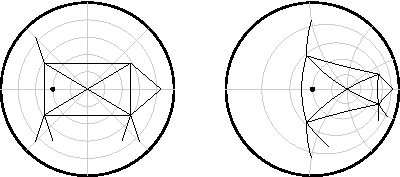
\includegraphics{figures/varphiplot}
\caption{What $\varphi_a$ does to the unit disc when $a=-0.4$.   The positions of $a$ and $0=\varphi_a(a)$ are marked with dots.%
\label{fig:varphiplot}}
\end{myfig}

\begin{prop}
If $f \in \operatorname{Aut}(\D)$, then there exists an $a \in \D$
and $\theta \in \R$ such that
\begin{equation*}
f(z) = e^{i\theta} \frac{z-a}{1-\bar{a}z} = e^{i\theta} \varphi_a(z).
\end{equation*}
\end{prop}

\begin{proof}
Suppose $f(0) = a$.
Consider $g = \varphi_a \circ f$, which is a biholomorphism,
and $g(0) = 0$ as
$\varphi_a(a) = 0$.
As in the proof of Schwarz's lemma, we find a holomorphic $h(z)$
such that $g(z) = z h(z)$.  By
Schwarz's lemma, if $z \in \D \setminus \{ 0 \}$, then
\begin{equation*}
\sabs{h(z)} = \frac{\sabs{g(z)}}{\sabs{z}} \leq 1 .
\end{equation*}
Consequently, $h$ is a map of the disc to the closed disc.

But $h$ can have no zeros:
$h(z) = \frac{g(z)}{z}$ cannot be zero for $z \not= 0$ as $g$ is injective
and it cannot have a zero at $z=0$
as $h(0) = \lim_{z\to 0} \frac{g(z)}{z} = g'(0) \not= 0$.  As $g$ is a biholomorphism, $g^{-1}$ is
continuous. So $g^{-1}(K)$ is compact for any compact $K \subset \D$.
In other words, $\sabs{g(z)}$ must approach $1$ as $z$
approaches the boundary $\partial \D$.
Then so must $\sabs{h(z)}$.
The function
$\sabs{h(z)}$ must, therefore, attain a minimum inside $\D$, or in other
words $\babs{\frac{1}{h(z)}}$ must attain a maximum inside $\D$.  So $h(z)$
is a constant, and $g(z) = \alpha z$ for some constant $\alpha$.
Clearly, 
$\sabs{\alpha} = 1$ or $\alpha = e^{i\theta}$.  Applying
$\varphi_{-a}$ to both sides of $e^{i\theta} z = \varphi_a \circ f$
we obtain
$f(z) = \varphi_{-a}(ze^{i\theta})
= e^{i \theta} \varphi_{-ae^{-i\theta}}(z)$.
\end{proof}

\begin{exbox}
\begin{exercise}
Justify the claim in the proof.  If a continuous
$g \colon \D \to \D$ is such that $g^{-1}(K)$ is compact
for every compact $K \subset \D$, then if $\{ z_n \}$ is a sequence
in $\D$ such that $\sabs{z_n} \to 1$, then
$\sabs{g(z_n)} \to 1$.
\end{exercise}

\begin{exercise}
Given two distinct $a,b \in \D$, show that there exists a unique 
$f \in \Aut(\D)$
such that $f(a) = b$ and $f(b) = a$.
\end{exercise}

\begin{exercise}
Prove that if $\bH = \{ z \in \C : \Im z > 0 \}$ is the upper half-plane
and $f \colon \bH \to \bH$ is an automorphism of $\bH$, then
\begin{equation*}
f(z) = \frac{a z +b}{c z + d}
\avoidbreak
\end{equation*}
for real numbers $a,b,c,d$ such that $ad-bc \not= 0$.
\end{exercise}

\begin{exercise}
Suppose $U \subset \C$ is a domain, $\overline{\D} \subset U$,
and $f \colon U \to \C$ is holomorphic.
Suppose $\sabs{f(z)}=1$ whenever $\sabs{z}=1$,
that is, $f(\partial \D) \subset \partial \D$.
Find a formula for $f$.  Use the following outline:
\begin{exparts}
\item
Show that $f$ must have finitely many zeros in $\D$.  That is, $f(z) = 0$
for at most finitely many $z \in \D$.
\item
Suppose that $f$ has no zeros in $\D$.  Prove that $f$ is constant
(and what sort of constant).
\item
If $f(a) = 0$, then prove that
$z \mapsto \frac{f(z)}{\phi_a(z)}$ is still holomorphic in $U$ and
still takes the circle to the circle.
\item
Now find a general formula for $f$.
\end{exparts}
\end{exercise}

\begin{exercise}
Suppose $f \colon \D \to \D$ is a holomorphic function with zeros at
$z_1,\ldots,z_n$, that is $f(z_\ell) = 0$ for $\ell=1,\ldots,n$.  Prove that
\begin{equation*}
\sabs{f(z)} \leq \sabs{\varphi_{z_1}(z)  
\varphi_{z_2}(z)
\cdots
\varphi_{z_n}(z)} .
\end{equation*}
\end{exercise}

\begin{exercise}
Prove the \emph{\myindex{Schwarz--Pick lemma}}:
If $f \colon \D \to \D$ is holomorphic, then
\begin{equation*}
\abs{
\frac{f(z)-f(\zeta)}{1-\overline{f(\zeta)}f(z)}
}
\leq
\abs{
\frac{z-\zeta}{1-\widebar{\zeta}z} 
}
\qquad
\text{and}
\qquad
\frac{\abs{f'(z)}}{1-\abs{f(z)}^2} \leq
\frac{1}{1-\abs{z}^2}
\end{equation*}
for all $z,\zeta \in \D$.
If equality holds in one of the 
inequalities for some $z \not= \zeta$,
then $f$ is an automorphism of $\D$.
Conversely if $f$ is an automorphism of $\D$,
then equality holds in both inequalities for
all $z,\zeta \in \D$.
\end{exercise}
\end{exbox}

\pagebreak[0]
In particular, the Schwarz--Pick lemma gives a bound on the derivative
at all points.  If
$f \colon \D \to \D$ is holomorphic, nonconstant, and $f(a) = b$,
then
\begin{equation*}
\sabs{f'(a)} \leq
\frac{1-\sabs{b}^2}{1-\sabs{a}^2} .
\end{equation*}
If equality holds, then $f(z) = \varphi_{-b}\bigl( e^{i\theta} \varphi_a(z)
\bigr)$ for some $\theta \in \R$.


%%%%%%%%%%%%%%%%%%%%%%%%%%%%%%%%%%%%%%%%%%%%%%%%%%%%%%%%%%%%%%%%%%%%%%%%%%%%%%
%%%%%%%%%%%%%%%%%%%%%%%%%%%%%%%%%%%%%%%%%%%%%%%%%%%%%%%%%%%%%%%%%%%%%%%%%%%%%%
%%%%%%%%%%%%%%%%%%%%%%%%%%%%%%%%%%%%%%%%%%%%%%%%%%%%%%%%%%%%%%%%%%%%%%%%%%%%%%

\chapter{The Logarithm and Cauchy} \label{ch:log}

\begin{myepigraph}
Never doubt the courage of the French. They were the ones who discovered that snails are edible.

---Doug Larson
\end{myepigraph}

%%%%%%%%%%%%%%%%%%%%%%%%%%%%%%%%%%%%%%%%%%%%%%%%%%%%%%%%%%%%%%%%%%%%%%%%%%%%%%

\section{The logarithm and the winding number}
\label{sec:log}

\subsection{The logarithm}

Let us ponder over the primitives of $z^n$ for $n \in \Z$.\footnote{It appears,
doesn't it, that elementary complex analysis is the study of $z^n$.}
When $n \geq 0$, 
then $z^n$ is defined in the entire plane, and a primitive is
simply $\frac{z^{n+1}}{n+1}$.  If $n < -1$, then $z^n$ is defined
in the punctured plane $\C \setminus \{0\}$, but again
a primitive is $\frac{z^{n+1}}{n+1}$.  What about $z^{-1} =
\nicefrac{1}{z}$?  It has a primitive, but never defined in
the entire punctured plane.

We demonstrated that in any star-like domain, a holomorphic function has a
primitive.  Consider the so-called \emph{\myindex{slit plane}}
\begin{equation*}
U = \C \setminus (-\infty,0] = \C \setminus \bigl\{ z \in \C : \Re z \leq 0 , \Im z = 0 \bigr\}.
\end{equation*}
It is a star-like domain and
so there exists a
primitive for $\nicefrac{1}{z}$ in $U$.
If we
require that this primitive is $0$ at $z=1$,
we get a function
\glsadd{not:Log}%
\begin{equation*}
\operatorname{Log} \colon U \to \C ,
\end{equation*}
called the \emph{\myindex{principal branch}} of the logarithm.
We saw another gadget before called the \myquote{principal branch,} 
the principal branch of the argument, $\Arg$.  Let us show that
\begin{equation*}
\Log z = \log \sabs{z} + i \Arg z ,
\end{equation*}
where $\log \sabs{z}$ is just the standard real logarithm of $\sabs{z}$.
Set $L(z) = \log \sabs{z} + i \Arg z$, and let us show that $L = \Log$.
Observe
\begin{equation*}
e^{L(z)}
=
e^{\log \sabs{z}} e^{i \Arg z}
=
\sabs{z} e^{i \Arg z} = z .
\end{equation*}
So $L$ is the inverse of the exponential, at least for $z \in U$.
This means in particular that $L$ is holomorphic by the inverse function
theorem.
Take the derivative of both sides of $z = e^{L(z)}$,
\begin{equation*}
1 = L'(z) e^{L(z)} = L'(z) z .
\end{equation*}
Et voil\`a!\footnote{Cauchy was French, n'est pas?}
We have $L'(z) = \nicefrac{1}{z}$, so $L = \Log$.

If we use a different branch of the argument we get another
antiderivative of $\nicefrac{1}{z}$.  We 
make the definition
\glsadd{not:log}%
\begin{equation*}
\log z \overset{\text{def}}{=} \log \sabs{z} + i \arg z .
\end{equation*}
This definition is totally bonkers at first glance.  First, the $\log$ on the
left is a different $\log$ than the $\log$ on the right.  On the right, it is the
standard real $\log$, that is, $\log \colon (0,\infty) \to \R$,
where $\log 1 = 0$.
But the $\log$ on the left
is not even a function, it has infinitely many values for every $z$,
since the $\arg$ on the right-hand side has infinitely many values.
The value of $\log (-1)$ is $\pi i$, but also $-\pi i$, $3\pi i$,
or $(\pi + 2\pi k)i$ for any $k \in \Z$.  So $\log$ is a function just as much
as $\arg$ is a function.  See \figureref{fig:loggraph}.
The double duty of \myquote{$\log$} is almost never a
problem and it is generally clear which $\log$ one is talking about based on
what sort of things are being plugged into it.


\begin{myfig}
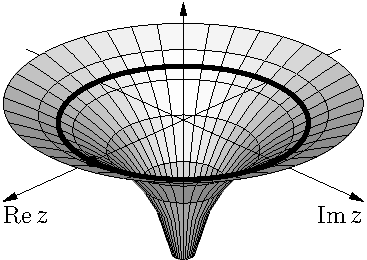
\includegraphics{figures/logrealgraph}
\qquad
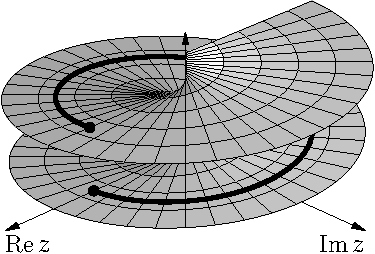
\includegraphics{figures/arggraph2}
\caption{\myquote{Graphs} of the real part (left) and imaginary part (right)
of the complex logarithm $\log z = \log \sabs{z} + i \arg z$.  The imaginary
part is an infinite spiral, only two turns are pictured.  A path on the
graph around the unit circle is marked.\label{fig:loggraph}}
\end{myfig}

While $\log$ is not really a function---it is a multivalued
function\footnote{%
Cauchy: Quel Malheur!  Je d{\'e}teste le logarithme! Je veux devenir plombier.}---it is
the definition that we want.
The principal branch,
useful when one wants to get some actual numbers, is often not what we
need; it is not as useful as one would think.
And beware that computers like to give back the principal branch even 
when it doesn't make any sense.

So how do we use $\log$?  Well it comes up in line integrals, which are used
to count and classify zeros and/or singularities of functions, or vice
versa---zeros and singularities are used to compute line integrals.
Let us compute the integral of $\nicefrac{1}{z}$ around the unit
circle $\partial \D$, oriented counterclockwise as usual (parametrized
by $e^{it}$).  Suppose we start and end the integration at 
$z=1$:
\begin{equation*}
\int_{\partial \D} \frac{1}{z} \, dz
= \log 1 - \log 1 = 2\pi i.
\end{equation*}
That makes no sense, no?  Well, it should really only be done
with quotation marks:
\begin{equation*}
\int_{\partial \D} \frac{1}{z} \, dz
\enspace
\text{``$=$''}
\enspace
\log 1 - \log 1
\enspace
\text{``$=$''}
\enspace
2\pi i.
\end{equation*}
That's a lot better,
no?\footnote{Non! Je veux aussi devenir plombier maintenant!}
The equalities are only true morally.
Interpreted correctly, it is exactly what is happening.  You really do subtract
one of the values of $\log 1$ from another value of $\log 1$.  To figure
out which from which, start with say $\log 1 = 0$, and follow the
function along the circle slowly and notice that $i \arg z$ grows from $0$ to
$2\pi i$.  So the $\log 1$ at the end is $2 \pi i$.  See the path
marked on \figureref{fig:loggraph}, the jump in the imaginary part between
the beginning and the end is precisely that $2\pi i$.

To make working with $\log$ easier, we usually talk about a
\emph{\myindex{branch of the logarithm}}.  So $L \colon U \to \C$ is a branch
of the logarithm if $L$ is holomorphic, $L'(z) = \nicefrac{1}{z}$, and $L(z)$ is equal
to some value of $\log z$ for every $z \in U$.  It is not possible to define
a branch of the logarithm in every $U$, but for example we can do it in every
star-like $U$ where $0 \notin U$.  In general, one can define a branch of
the logarithm in every simply connected domain, that is, a domain without holes,
that does not contain zero.
More on this later.  Similarly we define branches of $\log (z-p)$,
a primitive of $\frac{1}{z-p}$, in which case the domain
should not contain $p$.

We may also talk about branches more loosely, and talk
about following them along a path.  That doesn't mean that we really define
a single branch, it means that we define a branch in some small open set,
follow its values for a while, then switch to another branch that 
happens to agree with the first branch at least at the point where we
switch.  See \figureref{fig:followbranch}.  This is really what we did in the
\myquote{computation} above.  We followed $\log$ from $1$ along the circle until we
ended up at $1$ again, and our branches that we followed ended up $2\pi i$
off.  We will see an example of this briefly.

%Used in two places
\begin{myfig}
\subimport*{figures/}{followbranch.pdf_t}
\caption{Following a branch.
The branches are defined in the discs
(they do not have to be discs).
Points where the branches are supposed to equal
are marked.\label{fig:followbranch}}
\end{myfig}

\begin{exbox}
\begin{exercise}
Suppose $a \in \C \setminus \{ 0 \}$, and
$R_a = \{ \lambda a \in \C : \lambda \geq 0 \}$
is the ray from the origin through $a$.  Prove
that there exists a branch of the $\log$ in $\C \setminus R_a$.
\end{exercise}

\begin{exercise}
For $n \in \N$ let $\gamma \colon [0,2\pi] \to \C$ be $\gamma(t) = e^{int}$,
the unit circle traversed $n$ times counterclockwise.  Compute
$\int_\gamma \frac{1}{z} \, dz$.  Argue by splitting up the integral
into pieces and using branches of the $\log$.
\end{exercise}

\begin{exercise}
Suppose
$U \subset \C$ is open with
$\partial \D \subset U$,
$f \colon U \to \C$ is holomorphic,
such that
$f(z)$ is never negative real or zero.
Compute
$\int_{\partial \D} \frac{f'(z)}{f(z)} \, dz$.
\end{exercise}

\begin{exercise}
Suppose $\gamma \colon [a,b] \to \C \setminus \{ 0 \}$ is a piecewise-$C^1$
path such that $\gamma(a) = \gamma(b) = -1$, but $\gamma(t)$ is never
negative real for any $t \in (a,b)$.  Using the principal branch of the
$\log$, prove that
\begin{equation*}
\int_\gamma \frac{1}{z} \, dz = -2\pi i, 0, \text{ or } 2\pi i.
\avoidbreak
\end{equation*}
Find an explicit $\gamma$ that achieves each of these possibilities.
\end{exercise}
\end{exbox}

\subsection{Winding numbers}

OK.  Let's get more rigorous.

\begin{defn}\label{defn:windingnumber}
Let $\Gamma$ be
a cycle,
and $p \notin \Gamma$.  Then
\glsadd{not:windnum}%
\begin{equation*}
n(\Gamma;p)
\overset{\text{def}}{=}
\frac{1}{2\pi i} \int_\Gamma \frac{1}{z-p} \, dz
\end{equation*}
is called the
\emph{\myindex{winding number}} of $\Gamma$ around $p$, or
the 
\emph{\myindex{index}} of $\Gamma$ with respect to $p$.
\end{defn}

Intuitively, the winding number is the number of times that $\Gamma$ winds
around $p$.  This intuition is confirmed by integrating
$\nicefrac{1}{z}$ for the path $e^{it}$ for $t \in [0,2\pi]$ to get
a winding number $1$ around $p=0$,
as it goes once counterclockwise direction around zero.  If we do
the integral with $e^{2it}$, we go around zero twice in the
counterclockwise direction, and the winding number really is $2$.  Similarly
if we use $e^{-it}$, then we go around zero once in the
clockwise direction, and the winding number is $-1$.

The first thing to observe is that the winding number is an integer.

\begin{prop} \label{prop:indexinteger}
Suppose $\Gamma$ is a cycle and $p \notin \Gamma$.  Then
$n(\Gamma;p)$ is an integer.
%\begin{equation*}
%n(\Gamma;p) = \frac{1}{2\pi i} \int_\Gamma \frac{1}{z-p} \, dz
%\avoidbreak
%\end{equation*}
%is an integer.
\end{prop}

The proof is to take a closed path $\gamma$
and to follow a branch of $\log$ around $\gamma$, and
see by how much it changes.  See \figureref{fig:followbranch}, where we
go all the way around a loop.  Since we follow the argument
and we go some number of times around $p$ along $\gamma$, the
argument changes by some multiple of $2\pi$.

\begin{proof}
A cycle is (equivalent to) a linear combination (over the integers) of closed paths,
so we only need to consider closed piecewise-$C^1$ paths.
Let $\gamma \colon [0,1] \to \C$ be the path.
The path $\gamma$ as a set is compact.  It can be covered by finitely many
discs $D_1,\ldots,D_n$, none of which contain $p$, and such that there is a
partition $0 = t_0 < t_1 < t_2 < \cdots < t_n = 1$ such that
$\gamma\bigl([t_{j-1},t_j]\bigr) \subset D_j$.  Each $D_j$ is star-like and
does not contain $p$,
so in each one there exists a branch of $\log (z-p)$, call it $L_j$,
such that $L_j\bigl(\gamma(t_j)\bigr) = L_{j+1}\bigl(\gamma(t_j)\bigr)$.
Pick $L_1$ arbitrarily, then pick $L_2,\ldots,L_n$ accordingly.
Call $z_0 = \gamma(0) = \gamma(1)$.  So
\begin{multline*}
n(\gamma;p)
=
\frac{1}{2\pi i} \int_\gamma \frac{1}{z-p} \, dz
=
\frac{1}{2\pi i} \int_0^1 \frac{\gamma'(t)}{\gamma(t)-p} \, dt
=
\frac{1}{2\pi i} \sum_{j=1}^n \int_{t_{j-1}}^{t_j} \frac{\gamma'(t)}{\gamma(t)-p} \, dt
\\
=
\frac{1}{2\pi i} \sum_{j=1}^n L_j\bigl(\gamma(t_j)\bigr) -
L_j\bigl(\gamma(t_{j-1})\bigr)
=
\frac{1}{2\pi i} \bigl( L_n(z_0) - L_1(z_0) \bigr) .
\end{multline*}
As $L_n$ and $L_1$ are both branches of $\log$, their difference is
$2\pi k i$ for some $k \in \Z$, as each is $\log\sabs{z_0} + i \arg z_0$ for some value of
$\arg$.
\end{proof}

\begin{exbox}
\begin{exercise}
Fill in the details in the existence of the partition.  That is, once you
cover $\gamma$ by finitely many discs that do not contain $p$ show that
the partition $t_0,\ldots,t_n$ exists.  Hint: Some of the discs may
\myquote{repeat,} but make sure that you do not get \myquote{stuck} before reaching 1.
\end{exercise}
\end{exbox}

The second thing to observe is that $n(\Gamma;z)$ is constant as long as we
do not cross $\Gamma$.

\begin{prop} \label{prop:windingconstant}
Given a cycle $\Gamma$,
the function $z \mapsto n(\Gamma;z)$ is constant on the
topological components of $\C \setminus \Gamma$.
Furthermore, $n(\Gamma;z) = 0$ for $z$ on the unbounded component
of $\C \setminus \Gamma$.
\end{prop}

As $\Gamma$ is compact, there must be a unique unbounded component
of the complement $\C \setminus \Gamma$, and possibly several bounded
components.
See \figureref{fig:indexconstant} for example.

\begin{myfig}
\subimport*{figures/}{indexconstant.pdf_t}
\caption{Components of $\C \setminus \Gamma$ with the 
winding number around points in those components
marked.\label{fig:indexconstant}}
\end{myfig}

\begin{proof}
Let us show that the function
\begin{equation*}
p \mapsto n(\Gamma;p) = \frac{1}{2\pi i} \int_\Gamma \frac{1}{z-p} \, dz
\end{equation*}
is continuous on $\C \setminus \Gamma$.
Fix $p_0 \in \C \setminus \Gamma$, and let
\glsadd{not:distancetoset}%
$d = d(p_0,\Gamma)$ be the
distance from 
$p_0$ to $\Gamma$, namely
$d = \inf \bigl\{ \sabs{z-p_0} : z \in \Gamma \bigr\}$.
As $\Gamma$ is compact, $d > 0$.  
For any $p \in \Delta_{d/2}(p_0)$, we have $\sabs{z-p} \geq
\nicefrac{d}{2}$ for every $z \in \Gamma$.  Let $\ell$ be the length of
$\Gamma$, that is $\ell = \int_\Gamma \sabs{dz}$.  Then,
\begin{equation*}
\begin{split}
\abs{n(\Gamma;p_0)-n(\Gamma;p)}
=
\abs{\frac{1}{2\pi i} \int_\Gamma \frac{p_0-p}{(z-p_0)(z-p)} \, dz}
& \leq
\frac{1}{2\pi} \int_\Gamma \frac{\sabs{p_0-p}}{\sabs{z-p_0}\sabs{z-p}} \, \sabs{dz}
\\
& \leq 
\frac{\ell}{\pi {d}^2} \sabs{p_0-p} .
\end{split}
\end{equation*}
So, $n(\Gamma;p)$ is a continuous function of $p$.
As it is continuous
and integer-valued, it is constant on every connected component of
$\C \setminus \Gamma$ (the set where it is defined).

For any $p \in \C \setminus \Gamma$,
\begin{equation*}
\sabs{n(\Gamma;p)} \leq \frac{1}{2\pi} \int_\Gamma \frac{1}{\sabs{z-p}} \,
\sabs{dz} \leq \frac{1}{2\pi} \frac{\ell}{d(p,\Gamma)} .
\end{equation*}
On the unbounded component---as $\Gamma$ is compact---there are $p$
with $d(p,\Gamma)$ arbitrarily large, so $n(\Gamma;p)$ is arbitrarily small
on this component.  As it is constant, it is zero.
\end{proof}

\begin{exbox}
\begin{exercise}%[\neededexmark]
\label{exercise:windingcircle}
Show that $n\bigl(\partial \Delta_r(p);z\bigr) = 0$ if $z \notin
\overline{\Delta_r(p)}$ and 
$n\bigl(\partial \Delta_r(p);z\bigr) = 1$ if $z \in \Delta_r(p)$.
\end{exercise}

\begin{exercise}
Let $n \in \Z$ and $\gamma \colon [0,2\pi] \to \C$, where
$\gamma(t) = p + re^{in t}$ be a path, a path that goes $n$ times
counterclockwise around $\partial \Delta_r(p)$.
Prove that
$n\bigl(\gamma;z\bigr) = n$ if $z \in \Delta_r(p)$.
\end{exercise}

\begin{exercise}%[\neededexmark]
\label{exercise:windingcircles}
Suppose $0 < r_1 < r_2 < \infty$.
Let $\Gamma = \partial \Delta_{r_2}(p) - \partial \Delta_{r_1} (p)$
(that is, the outside circles goes counterclockwise, the inside circle goes
clockwise).
Prove that if $z \in \C$ is such that $\sabs{z-p} < r_1$, then
$n(\Gamma;z) = 0$.  If $r_1 < \sabs{z-p} < r_2$, then
$n(\Gamma;z) = 1$.  If $r_2 < \sabs{z-p}$, then
$n(\Gamma;z) = 0$.
\end{exercise}

\begin{exercise}%[\optneededexmark]
\label{exercise:rayktimes}
Suppose $\gamma \colon [a,b] \to \C$ is a closed $C^1$ path such that
$\gamma(a) = \gamma(b)$ is some real negative number.  Suppose
that $\gamma(t)$ is real and negative for only $k$ distinct $t$ (that
includes $t=a$ and $t=b$, so $k \geq 2$), and whenever $\gamma(t)$ is real and negative,
then $\Im \gamma'(t) < 0$.  Prove that $n(\gamma;0) = k-1$.  Hint: Use
the principal branch.
\end{exercise}
\end{exbox}


%%%%%%%%%%%%%%%%%%%%%%%%%%%%%%%%%%%%%%%%%%%%%%%%%%%%%%%%%%%%%%%%%%%%%%%%%%%%%%

\section{Homology versions of Cauchy}

\begin{defn}
Let $U \subset \C$ be a domain and $\Gamma$
a cycle
in $U$
such that $n(\Gamma;p) = 0$ for all $p \in \C \setminus U$,
 then we
say $\Gamma$ is \emph{\myindex{homologous to zero} in $U$}.
\end{defn}

What homologous to zero means is that $\Gamma$ does not wind around any
point in the complement of $U$.
Do note that \myquote{homologous to zero} does not mean
\myquote{equivalent to zero.}
For instance, if $U = \C$, then every $\Gamma$ is homologous to zero trivially.
Also note the dependence on $U$.  The unit circle is homologous to zero in
$U = \C$, but it is not homologous to zero in $U = \C \setminus \{ 0 \}$.

\begin{thm}[Cauchy integral formula (homology version)]
\index{Cauchy integral formula!homology}
\label{thm:CIFhomology}
Suppose $U \subset \C$ is open, $f \colon U \to \C$ is holomorphic, and
$\Gamma$ is
a cycle
in $U$
homologous to zero in $U$.
Then for $z \in U \setminus \Gamma$,
\begin{equation*}
n(\Gamma;z)
f(z)
=
\frac{1}{2\pi i}
\int_{\Gamma}
\frac{f(\zeta)}{\zeta-z}
\,
d \zeta .
\end{equation*}
\end{thm}

Before we prove the theorem let us remark
that in the proof, rather strangely, we will define an entire
function (even though $U$ may be small) and then we will use
Liouville's theorem (\thmref{thm:Liouville}).

\begin{proof}
Define $g \colon U \times U \to \C$ by
\begin{equation*}
g(\zeta,z) =
\begin{cases}
\frac{f(\zeta)-f(z)}{\zeta-z} & \text{if } \zeta \not= z , \\
f'(\zeta)                 & \text{if } \zeta = z .
\end{cases}
\end{equation*}

\begin{exbox}
\begin{exercise}
Prove that $g(\zeta,z)$ is continuous in $U \times U$, and that
the function $z \mapsto g(\zeta,z)$ is holomorphic for every fixed $\zeta \in U$.
Hint: The only mildly tricky piece of this proof is showing that $z \mapsto
g(\zeta,z)$ is
holomorphic at $z=\zeta$.
\end{exercise}
\end{exbox}

Let
\begin{equation}\label{eq:CIFdefofh}
h(z) = 
\begin{cases}
\int_\Gamma g(\zeta,z) \, d\zeta & \text{if } z \in U , \\
\int_\Gamma \frac{f(\zeta)}{\zeta-z} \, d\zeta & \text{if } z \not \in
\Gamma \text{ and } n(\Gamma;z) = 0 .
\end{cases}
\end{equation}
As $n(\Gamma;z) = 0$ for all $z \in \C \setminus U$
($\Gamma$ is homologous to zero)
the function $h(z)$ is defined for every $z \in \C$.
Unfortunately, at some points
we have two definitions.
To show that $h(z)$ is well-defined, we must show that if
$n(\Gamma;z) = 0$ and $z \in U$, then the two definitions agree.
Consider such a $z$ (in particular $z \notin \Gamma$).  Then,
\begin{equation*}
\int_\Gamma g(\zeta,z) \, d\zeta
=
\int_\Gamma \frac{f(\zeta)-f(z)}{\zeta-z} \, d\zeta
=
\int_\Gamma \frac{f(\zeta)}{\zeta-z} \, d\zeta
-
f(z) n(\Gamma;z)
=
\int_\Gamma \frac{f(\zeta)}{\zeta-z} \, d\zeta .
\end{equation*}
So $h \colon \C \to \C$ is well-defined.

Next we show that $h$ is
holomorphic.
Holomorphicity is a local property, so we only need to prove it 
in a neighborhood of every point.
The set where $n(\Gamma;z) = 0$ is open as it is a
union of topological components of $\C \setminus \Gamma$.
So each point has a neighborhood where $h$ is defined
entirely by one or the other expression in \eqref{eq:CIFdefofh}.
Given any point,
take a neighborhood where one of the expressions defines
$h$ and apply \corref{cor:holfuncbyintegral}.

The unbounded component of $\C \setminus \Gamma$ is contained in the
set where $n(\Gamma;z) = 0$, so on this component, $h$ is defined by the
second expression.  Consider a $z$ in this component.
Suppose $\sabs{f(\zeta)} \leq M$ for $\zeta \in \Gamma$, let $\ell$ be the length of
$\Gamma$, and let $d(z,\Gamma)$ be the distance of $z$ to $\Gamma$.
\begin{equation*}
\sabs{h(z)}
=
\abs{
\int_\Gamma \frac{f(\zeta)}{\zeta-z} \, d\zeta
}
\leq
\int_\Gamma \abs{\frac{f(\zeta)}{\zeta-z}} \, \sabs{d\zeta}
\leq
\frac{M \ell}{d(z,\Gamma)} .
\end{equation*}
As $z \to \infty$, so does $d(z,\Gamma) \to \infty$, and so $h(z) \to 0$.
In particular, $h$ is an entire bounded function and
Liouville says that $h$ is constant, and that constant must be zero.
So suppose $z \in U \setminus \Gamma$.  Then
\begin{equation*}
0 = h(z) =
\int_\Gamma \frac{f(\zeta)-f(z)}{\zeta-z} \, d\zeta
=
\int_\Gamma \frac{f(\zeta)}{\zeta-z} \, d\zeta
-
f(z) n(\Gamma;z) . \qedhere
\end{equation*}
\end{proof}

Cauchy's theorem actually follows immediately using the integral formula.

\begin{thm}[Cauchy's theorem (homology version)]
\index{Cauchy's theorem!homology}%
\label{thm:CThomology}%
Suppose $U \subset \C$ is open,
$f \colon U \to \C$ is holomorphic,
and $\Gamma$ is
a cycle
in $U$
homologous to zero in $U$.
Then
\begin{equation*}
\int_\Gamma f(z) \, dz = 0 .
\end{equation*}
\end{thm}

\begin{proof}
Fix $z \in U \setminus \Gamma$.  Apply 
the Cauchy integral formula for the function $\zeta \mapsto
(\zeta-z)f(\zeta)$ at $\zeta=z$:
\begin{equation*}
0 = n(\Gamma;z) (z-z)f(z) =
\frac{1}{2\pi i} \int_\Gamma \frac{(\zeta-z)f(\zeta)}{\zeta-z} \, d\zeta
=
\frac{1}{2\pi i} \int_\Gamma f(\zeta) \, d\zeta . \qedhere
\end{equation*}
\end{proof}

\begin{defn}
Two cycles
$\Gamma_0$ and $\Gamma_1$ in $U
\subset \C$ are \emph{\myindex{homologous}} in $U$
if $n(\Gamma_0;p) = n(\Gamma_1;p)$ for all $p \in \C \setminus U$.
\end{defn}

Equivalently, $\Gamma_0$ and $\Gamma_1$ are homologous in $U$ if
$n(\Gamma_0 - \Gamma_1;p) = 0$ for all $p \in \C \setminus U$,
that is, $\Gamma_0-\Gamma_1$ is homologous to zero in $U$.

\begin{cor} \label{cor:homologoussameint}
Let $U \subset \C$ be open and $f \colon U \to \C$ holomorphic.
If two cycles
$\Gamma_0$ and $\Gamma_1$ in $U$
are homologous in $U$, then
\begin{equation*}
\int_{\Gamma_0} f(z)\, dz = 
\int_{\Gamma_1} f(z)\, dz .
\end{equation*}
\end{cor}

The proof is immediate by applying Cauchy's theorem to $\Gamma_0-\Gamma_1$.

\begin{exbox}
\begin{exercise}[Easy]
Suppose that $\Gamma$ is a cycle such that
$n(\Gamma;0) = k$.  Compute
\begin{equation*}
\int_{\Gamma} \frac{\cos z}{z} \, dz .
\end{equation*}
\end{exercise}

\begin{exercise}
Let $\Gamma$ be
a cycle in $\C \setminus \{ 0 \}$.
Prove that $\Gamma$ is homologous in $\C \setminus \{ 0 \}$
to $n \partial \D$ for some $n \in \Z$.
\end{exercise}

\begin{exercise} \label{exercise:H1U}
\begin{exparts}
\item
Show that being homologous in $U$ is an equivalence relation on cycles.
\item
Prove that the addition of cycles makes the set of equivelence classes
into an abelian group, the
first \emph{\myindex{homology group}}\index{first homology group} of $U$,
usually written $H_1(U)$.
\item
Compute $H_1(\C \setminus \{ 0 \})$ (that is,
find what group is it isomorphic to).
\end{exparts}
\end{exercise}

\begin{exercise}
Prove that the two theorems
(the homology versions of Cauchy's theorem and the Cauchy integral formula)
are equivalent logically, that is, one follows
from the other.  We have already proved that the Cauchy integral formula
implies Cauchy's theorem.  So prove that
Cauchy's theorem implies the Cauchy integral formula.
\end{exercise}

\begin{exercise}
Let $U \subset \C$ is open and $\Gamma$ is a cycle in $U$
homologous to zero in $U$.
Suppose that $n(\Gamma;z_1) = k_1$ and  $n(\Gamma;z_2) = k_2$ for
some two distinct $z_1,z_2 \in U \setminus \Gamma$.
Let $f \colon U \setminus \{z_1,z_2\} \to \C$ be
holomorphic.
Suppose $0< \epsilon < \sabs{z_1-z_2}$ is small enough that
$\overline{\Delta_\epsilon(z_j)} \subset U$ for $j=1,2$,
and that
$\int_{\partial \Delta_\epsilon(z_1)} f(z) \, dz = A$ and 
$\int_{\partial \Delta_\epsilon(z_2)} f(z) \, dz = B$.
In terms of $k_1$, $k_2$, $A$, and $B$,
compute
\begin{equation*}
\int_{\Gamma} f(z) \, dz .
\end{equation*}
\end{exercise}
\end{exbox}


%%%%%%%%%%%%%%%%%%%%%%%%%%%%%%%%%%%%%%%%%%%%%%%%%%%%%%%%%%%%%%%%%%%%%%%%%%%%%%

\section{Simply connected domains}

A simply connected domain\footnote{%
There is no agreement among various mathematicians (I've asked a few) if
a (path-)disconnected set can be \myquote{simply connected.}
To avoid heated arguments with topologists of various stripes,
it's best to just not define the term for disconnected sets.
Hence, we only define it for domains.}
is one without any holes.  The following is
perhaps not the standard definition, but for domains in $\C$
(connected open sets)
it is equivalent to the correct one.
We will define the term \myquote{properly} once we get 
to homotopy.\footnote{Homotopy is in an optional section, which is the
reason why we make this \myquote{wrong} definition.}
We may sometimes say
\myquote{simply connected in the sense of homology}
to emphasize that we are using this particular definition.

\begin{defn} \label{defn:simplyconnected:homology}
A domain $U \subset \C$ is \emph{\myindex{simply connected}}
if every cycle in $U$
is homologous to zero in $U$.
\end{defn}

In other words, $U$ is simply connected
if $n(\Gamma;p) = 0$ for every cycle $\Gamma$ in $U$ and
every $p \in \C \setminus U$.
So in a simply connected domain, no cycle in $U$ can wind around any point
of $\C \setminus U$.  Examples of simply connected domains are $\C$, $\D$, or
$\bH$.  An example of a domain that is not simply connected is
$\C \setminus \{ 0 \}$.
See the exercises below.


\begin{exbox}
\begin{exercise}
\begin{exparts}
\item
Prove that every star-like domain (e.g., $\C$, $\D$, and $\bH$) in $\C$ is simply connected.
\item
Prove that $\C \setminus \{ 0 \}$ is not simply connected.
\end{exparts}
\end{exercise}

\begin{exercise}
Prove that if $U \subset \C$ is biholomorphic to $\D$, then $U$
is simply connected.
\end{exercise}

\begin{exercise}
Prove that $U \subset \C$ is simply connected if and only if
the first homology group
$H_1(U)$ is isomorphic to the trivial group $\{ 0 \}$.
See \exerciseref{exercise:H1U}.
\end{exercise}
\end{exbox}

A special (but common) case of the homology version of Cauchy,
\thmref{thm:CThomology}, can be stated as the simply connected case of Cauchy.

\begin{thm}[Cauchy's theorem (simply connected version)]
\index{Cauchy's theorem!simply connected}%
Let $U \subset \C$ be a simply connected domain and $f \colon U \to \C$
holomorphic.  If $\Gamma$ is a cycle in $U$, then
\begin{equation*}
\int_\Gamma f(z) \, dz = 0 .
\end{equation*}
\end{thm}

The proof follows at once from \thmref{thm:CThomology},
since if $U$ is simply connected, then
every $\Gamma$ in $U$ is homologous to zero in $U$.
In simply connected domains,
as Cauchy's theorem holds for all cycles,
we have primitives (antiderivatives).

\begin{thm}
Let $U \subset \C$ be a simply connected domain and
let $f \colon U \to \C$ be holomorphic.  Then $f$ has a
primitive in $U$.
\end{thm}

\begin{proof}
Fix some $p \in U$. As $U$ is path connected, for every $z \in U$, pick
some piecewise-$C^1$ path $\gamma$ from $p$ to $z$
and define
\begin{equation*}
F(z) = \int_\gamma f(\zeta) \, d\zeta .
\end{equation*}
A priory, the function $F(z)$ depends on $\gamma$, but Cauchy's
theorem says that if $\alpha$ is another path from $p$ to $z$, then
\begin{equation*}
\int_\gamma f(\zeta) \, d\zeta -
\int_\alpha f(\zeta) \, d\zeta 
=
\int_{\gamma-\alpha} f(\zeta) \, d\zeta  =  0 .
\end{equation*}
So $F$ is well-defined without specifying the path.

Let us reduce the proof to the proof for 
star-like domains (\propref{prop:primitiveinstarlike1} and
\corref{cor:primitiveinstarlike}).
Let $q \in U$ be a point and consider a disc $\Delta_r(q) \subset U$
(which is star-like with respect to $q$ in particular).
We take $\gamma$ to be the path from $p$ to $q$.
As $F$ does not depend on the path taken, then for $z \in \Delta_r(q)$,
\begin{equation*}
F(z) =
\int_{\gamma+[q,z]} f(\zeta) \, d\zeta
=
\int_{\gamma} f(\zeta) \, d\zeta
+
\int_{[q,z]} f(\zeta) \, d\zeta .
\end{equation*}
The first term in the sum is a constant, and the second term is precisely
the primitive of $f$ from the proof of
\propref{prop:primitiveinstarlike1},
that is, a primitive in
$\Delta_r(q)$.
See \figureref{fig:anyantidef}.
\end{proof}

\begin{myfig}
\subimport*{figures/}{anyantidef.pdf_t}
\caption{Existence of primitive in a simply connected
domain with $\Delta_r(q)$ marked.\label{fig:anyantidef}}
\end{myfig}

\begin{cor} \label{cor:simplyconimpleslog}
Let $U \subset \C$ be a simply connected domain and
let $f \colon U \to \C$ be a nowhere zero holomorphic
function.  Then there exists a holomorphic $g \colon U \to \C$
such that
\begin{equation*}
e^{g(z)} = f(z) .
\end{equation*}
\end{cor}

In particular,
if $U \subset \C \setminus \{ 0 \}$ is a simply connected domain, then
%(let $f(z) = z$) 
there exists a branch of the logarithm, that is,
a holomorphic $L \colon U \to \C$ such that
\begin{equation*}
e^{L(z)} = z .
\end{equation*}

\begin{proof}
The function $\frac{f'(z)}{f(z)}$ is holomorphic on $U$.
Find a primitive $g(z)$.  Compute,
\begin{equation*}
\frac{d}{dz} \left[ \frac{e^{g(z)}}{f(z)} \right] =
\frac{ e^{g(z)} g'(z) f(z) - e^{g(z)} f'(z) }{{\bigl(f(z)\bigr)}^2}
=
\frac{ e^{g(z)} f'(z) - e^{g(z)} f'(z) }{{\bigl(f(z)\bigr)}^2}
=
0 .
\end{equation*}
Thus, $\frac{e^{g(z)}}{f(z)}$ is constant
(\propref{prop:zeroder}).  It follows that
there is a $C \in \C$ such that
\begin{equation*}
e^{g(z) + C} = f(z) .
\qedhere
\end{equation*}
\end{proof}

If we have the logarithm, we can take roots.

\begin{cor}
Let $U \subset \C$ be a simply connected domain,
let $f \colon U \to \C$ be a nowhere zero holomorphic
function, and let $k \in \N$.
Then there exists a holomorphic $g \colon U \to \C$
such that
\begin{equation*}
{\bigl(g(z)\bigr)}^k = f(z) .
\end{equation*}
\end{cor}

\begin{proof}
Find a $\psi \colon U \to \C$ such that $e^{\psi(z)} = f(z)$.  Let
$g(z) = e^{\frac{1}{k} \psi(z)}$.  Check:
\begin{equation*}
{\bigl(g(z)\bigr)}^k
=
{\left( e^{\frac{1}{k} \psi(z)} \right)}^k
=
e^{\psi(z)} = f(z) . \qedhere
\end{equation*}
\end{proof}

On the other hand, the existence of primitives or
Cauchy's theorem without restriction on $\Gamma$ or existence of logs guarantees
simply-connectedness.  In particular, we have the following set of equivalent
versions of simply-connectedness for domains.

\begin{prop}
Let $U \subset \C$ be a domain.  The following are equivalent:
\begin{enumerate}[(i)]
\item \label{thm:simplyconnected:i}
$U$ is simply connected (in the homology sense).
\item \label{thm:simplyconnected:ii}
Every holomorphic $f \colon U \to \C$ has a primitive.
\item \label{thm:simplyconnected:iii}
Every nowhere zero holomorphic $f \colon U \to \C$ there exists
a holomorphic $g \colon U \to \C$ such that $e^{g(z)} = f(z)$.
\item \label{thm:simplyconnected:iv}
$\frac{1}{z-p}$ has a primitive in $U$ for every $p \in \C \setminus U$.
\item \label{thm:simplyconnected:v}
For every holomorphic $f \colon U \to \C$ and every
cycle $\Gamma$ in $U$, we have
\begin{equation*}
\int_\Gamma f(z) \, dz = 0 .
\end{equation*}
\item \label{thm:simplyconnected:vi}
For every $p \in \C \setminus U$ and every
cycle $\Gamma$ in $U$, we have
\begin{equation*}
\int_\Gamma \frac{1}{z-p} \, dz = 0 .
\end{equation*}
\end{enumerate}
\end{prop}

\begin{proof}
The logic of the proof is the following diagram:
\begin{equation*}
\begin{tikzcd}[cramped, row sep=small]
& \text{\ref{thm:simplyconnected:ii}} \arrow[d, Rightarrow] \arrow[r, Rightarrow] &
\text{\ref{thm:simplyconnected:iii}} \arrow[d, Rightarrow] \\
\text{\ref{thm:simplyconnected:i}} \arrow[ur, Rightarrow] & 
\text{\ref{thm:simplyconnected:v}} \arrow[d, Rightarrow] &
\text{\ref{thm:simplyconnected:iv}} \arrow[dl, Rightarrow] \\
& \text{\ref{thm:simplyconnected:vi}} \arrow[ul, Leftrightarrow] &
\end{tikzcd}
\end{equation*}
We proved
\ref{thm:simplyconnected:i} $\Rightarrow$
\ref{thm:simplyconnected:ii} above,
and
\ref{thm:simplyconnected:ii} $\Rightarrow$
\ref{thm:simplyconnected:iii}
is the same as proof of \corref{cor:simplyconimpleslog}.
Next, suppose \ref{thm:simplyconnected:iii} is true.  Find a $g$ such that
$e^{g(z)} = z-p$, and differentiate
\begin{equation*}
1 = 
\frac{d}{dz} \left[
z-p
\right]
=
\frac{d}{dz} \left[
e^{g(z)}
\right]
=
e^{g(z)} g'(z)
=
(z-p) g'(z) .
\end{equation*}
So \ref{thm:simplyconnected:iv} follows.
%\ref{thm:simplyconnected:iv} is immediate.
Using Cauchy's theorem for derivatives (\corref{cor:cauchyforders}),
\ref{thm:simplyconnected:iv} implies
\begin{equation*}
\int_\Gamma \frac{1}{z-p} \, dz = 0 
\end{equation*}
for every $p \in \C \setminus U$,
and hence 
\ref{thm:simplyconnected:vi} is true.
As 
\begin{equation*}
n(\Gamma;p) = 
\frac{1}{2\pi i}
\int_\Gamma \frac{1}{z-p} \, dz ,
\end{equation*}
\ref{thm:simplyconnected:vi} is simply a restatement of
\ref{thm:simplyconnected:i}.
Again by Cauchy's theorem for derivatives,
\ref{thm:simplyconnected:ii} $\Rightarrow$
\ref{thm:simplyconnected:v}.
Finally, \ref{thm:simplyconnected:v} $\Rightarrow$
\ref{thm:simplyconnected:vi} is immediate.
\end{proof}

The existence of roots, in particular the square root, can also be put on
the list, but as the proof of that fact follows easily from the argument principle
(\thmref{thm:argprinc} from the future),
we will leave it as an exercise in that upcoming section.

There is a simple topological criterion for
simply-connectedness of domains in the complex plane.
The theorem is actually an \myquote{if and only if,} but the other
direction is more difficult and so let's just prove the easy direction
at this point.
The harder direction will be much easier to prove once we have the Riemann
mapping theorem, see \subsectionref{subsec:patharoundK}, so we will
prove it there.

\begin{prop} \label{prop:scbycomplementeasy}
Let $U \subset \C$ be a domain.  If
$\C_\infty \setminus U$ is connected, then $U$ is simply connected.
\end{prop}

\begin{proof}
Take $S = \C_\infty \setminus U$ and let $\Gamma$ be a cycle in $U$.
The function $\varphi(z)= n(\Gamma;z)$ is continuous on 
$\C \setminus \Gamma$,
therefore $\varphi$ is a continuous function on $S \setminus \{
\infty \}$.  On the unbounded component of $\C \setminus \Gamma$ the
function is zero, and so $\varphi$ is zero in a neighborhood of $\infty$ and so
if we set $\varphi(\infty) = 0$, the function is continuous
on $\C_\infty \setminus \Gamma$.  As $S$ is connected
it is contained in
a single component of $\C_\infty \setminus \Gamma$ so $\varphi$ is
constant on $S$.  As $\varphi(\infty) = 0$, $\varphi|_S \equiv 0$.  In
other words, $U$ is simply connected.
\end{proof}

It is important to use $\C_\infty$ and not $\C$ in the proposition.
If $U = \C \setminus \{ 0 \}$ is the punctured plane, then
$\C \setminus U = \{ 0 \}$ is connected, but 
$\C_\infty \setminus U = \{ 0, \infty \}$ is not connected.

\begin{exbox}
\begin{exercise}
Suppose $U \subset \C$ is a domain, $\partial \Delta_r(p) \subset U$,
but there is a $z \in \Delta_r(p)$ such that $z \notin U$.
Prove that $U$ is not simply connected.
\end{exercise}

\begin{exercise}
Let $K \subset \C$ be nonempty and compact.
Prove that the unbounded component of $\C \setminus K$ is not a
simply connected domain.
\end{exercise}

\begin{exercise}
Let $U_1,U_2 \subset \C$ be two simply connected domains such that $U_1 \cap
U_2$ is nonempty and connected.
Prove that $U = U_1 \cup U_2$ is a simply connected domain.
\end{exercise}

\begin{exercise}
Let $U_1,U_2 \subset \C$ be two simply connected domains such that $U_1 \cap
U_2$ is nonempty and connected.
Prove that $U = U_1 \cap U_2$ is a simply connected domain.
Note: This is true in the plane but it is no longer true in the Riemann
sphere.
\end{exercise}

\begin{exercise}
Find two nonempty simply connected domains
$U_1,U_2 \subset \C$ such that $U_1 \cap U_2$ is nonempty and both
\begin{exnumparts}
\item
$U_1 \cup U_2$ is not a simply connected domain.
\item
$U_1 \cap U_2$ is not a simply connected domain (emphasis on domain).
\end{exnumparts}
\end{exercise}

\begin{exercise}
Suppose $U \subset \C$ is a simply connected domain such that $0 \notin U$,
there exist some positive real numbers in $U$, and that $r \in \R$.
Show that there exists a holomorphic $f \colon U \to \C$ such
that $f(x) = x^r$ for all $x > 0$ in $U$.
\end{exercise}

\begin{exercise}
Find a simply connected domain $U \subset \C$ such that $\C \setminus U$
has infinitely many components ($\C_\infty \setminus U$ is still going to
have just one component).
\end{exercise}
\end{exbox}

%%%%%%%%%%%%%%%%%%%%%%%%%%%%%%%%%%%%%%%%%%%%%%%%%%%%%%%%%%%%%%%%%%%%%%%%%%%%%%

\section{Laurent series}

One can also define a series for a holomorphic function around a hole, or a singularity.

\begin{defn}
Given $0 \leq r_1 < r_2 \leq \infty$ and $p \in \C$, define
\glsadd{not:annulus}%
\begin{equation*}
\ann(p;r_1,r_2)
\overset{\text{def}}{=}
\{ z \in \C : r_1 < \sabs{z - p} < r_2 \} .
\end{equation*}
When $0 < r_1 < r_2 < \infty$ we call this set an
\emph{\myindex{annulus}}\footnote{%
Q: What do you call a banana with a hole?
A: A banannulus.}.
\end{defn}

A common case is when $r_1 = 0$, that is,
the punctured disc
\begin{equation*}
\ann(p;0,r) = \Delta_r(p) \setminus \{ p \} .
\end{equation*}
When $r_2 = \infty$ on the other hand,
$\ann(p;r,\infty) = \C \setminus \overline{\Delta_{r}(p)}$ (if $r > 0$).  We will,
however, avoid temptation calling $\ann(p;r,\infty)$ an \myquote{annulus.}%
\footnote{\myquote{Holey plane} perhaps?  A punctured disc also ought not to be
called an \myquote{annulus,} and calling $\ann(0;0,\infty) = \C \setminus
\{ 0 \}$ an \myquote{annulus} is right out!}

\begin{thm}[\myindex{Existence of Laurent series}]
\index{Laurent series!existence}%
\label{thm:laurent}%
Suppose that $0 \leq r_1 < r_2 \leq \infty$ and
$f \colon \ann(p;r_1,r_2) \to \C$ is holomorphic.
Then there exist unique numbers $c_n \in \C$ for $n \in \Z$ such that
\glsadd{not:laurentser}%
\begin{equation*}
f(z) = \sum_{n=-\infty}^{\infty} c_n {(z-p)}^n ,
\end{equation*}
converging uniformly absolutely on compact subsets of
$\ann(p;r_1,r_2)$.  The numbers $c_n$ are given by
\begin{equation*}
c_n = 
\frac{1}{2\pi i}
\int_{\gamma}
\frac{f(z)}{{(z-p)}^{n+1}}
\,
dz  ,
\end{equation*}
where $\gamma$ is any circle of radius $s$, $r_1 < s < r_2$, centered at
$p$ oriented counterclockwise.
\end{thm}

Recall that convergence of a double series such as
\begin{equation*}
\sum_{n=-\infty}^{\infty} a_n
\end{equation*}
means
\begin{equation*}
\sum_{n=-\infty}^{\infty} a_n
=
\lim_{N\to -\infty}
\sum_{n=N}^{-1} a_n
+
\lim_{M\to \infty}
\sum_{n=0}^{M} a_n .
\end{equation*}
That is, the limits are taken independently.  However, for the series we
are interested in, we are generally talking
about absolute convergence, so the limit may be taken in any way,
and in any order.
When working with Laurent series in particular, we know even more.
Write a Laurent series as 
\begin{multline*}
\sum_{n=-\infty}^{\infty} c_n {(z-p)}^n
=
\sum_{n=0}^{\infty} c_n {(z-p)}^n
+
\sum_{n=-\infty}^{-1} c_n {(z-p)}^n
\\
=
\sum_{n=0}^{\infty} c_n {(z-p)}^n
+
\sum_{n=1}^{\infty} c_{-n} {\left(\frac{1}{z-p}\right)}^n .
\end{multline*}
So the Laurent series behaves like two power series: one in $z-p$ and one
in $\frac{1}{z-p}$.  You can therefore apply what you know about power
series.

\begin{proof}[Proof of the theorem]
Choose two numbers $s_1$ and $s_2$ such that $r_1 < s_1 < s_2 < r_2$.
Define the cycle
\begin{equation*}
\Gamma = \partial \Delta_{s_2}(p) - \partial \Delta_{s_1}(p) .
\end{equation*}
That is, $\Gamma$ goes around the larger ($s_2$) circle counterclockwise and
around the smaller ($s_1$) circle clockwise.
See \figureref{fig:twoannuli}.

\begin{myfig}
\subimport*{figures/}{twoannuli.pdf_t}
\caption{The two annuli, the smaller annulus is shaded darker.  The two
pieces of $\Gamma$ are noted with the circular arrows.\label{fig:twoannuli}}
\end{myfig}

If $q \in \C \setminus \ann(p;r_1,r_2)$, then $n(\Gamma;q) = 0$:
If $q$ is in the \myquote{hole} of the annulus $\ann(p;r_1,r_2)$, then
$n\bigl(\partial \Delta_{s_j}(p);q\bigr) = 1$ for both $j=1,2$, and 
if $q$ is outside the annulus altogether, then
$n\bigl(\partial \Delta_{s_j}(p);q\bigr) = -1$ for both $j=1,2$ 
(see \exerciseref{exercise:windingcircle} or
\exerciseref{exercise:windingcircles}).
So $\Gamma$ is homologous to zero in the annulus $\ann(p;r_1,r_2)$.
On the other hand if $q$ is in the (smaller) annulus $\ann(p;s_1,s_2)$,
then for similar reasons, $n(\Gamma;q) = 1$.

Via Cauchy's theorem (\thmref{thm:CThomology}), for every $z \in \ann(p;s_1,s_2)$,
\begin{equation*}
f(z) = 
\frac{1}{2\pi i}
\int_{\Gamma} \frac{f(\zeta)}{\zeta-z} \, d\zeta 
=
\frac{1}{2\pi i}
\int_{\partial \Delta_{s_2}(p)} \frac{f(\zeta)}{\zeta-z} \, d\zeta 
-
\frac{1}{2\pi i}
\int_{\partial \Delta_{s_1}(p)} \frac{f(\zeta)}{\zeta-z} \, d\zeta  .
\end{equation*}

Let us expand the two bits separately.  First
if $\zeta \in \partial \Delta_{s_2}$, then
$\babs{\frac{z-p}{\zeta-p}} = \frac{\sabs{z-p}}{s_2} < 1$ and so
we follow the logic of \thmref{thm:holpower}.  The reason that we can
swap the integral and the series limit is the same as in that theorem.
\begin{equation*}
\begin{split}
\frac{1}{2\pi i}
\int_{\partial \Delta_{s_2}(p)} \frac{f(\zeta)}{\zeta-z} \, d\zeta 
& =
\frac{1}{2\pi i}
\int_{\partial \Delta_{s_2}(p)} \frac{f(\zeta)}{\zeta-p}
\frac{1}{1-\frac{z-p}{\zeta-p}} \, d\zeta
\\
& =
\frac{1}{2\pi i}
\int_{\partial \Delta_{s_2}(p)} \frac{f(\zeta)}{\zeta-p}
\sum_{n=0}^\infty
{\left(\frac{z-p}{\zeta-p}\right)}^n \, d\zeta
\\
& =
\sum_{n=0}^\infty
\underbrace{
\left(
\frac{1}{2\pi i}
\int_{\partial \Delta_{s_2}(p)} \frac{f(\zeta)}{{(\zeta-p)}^{n+1}}
 \, d\zeta
\right)
}_{c_n}
{(z-p)}^n .
\end{split}
\end{equation*}

Similarly, 
if $\zeta \in \partial \Delta_{s_1}$, then
$\babs{\frac{\zeta-p}{z-p}} = \frac{s_1}{\sabs{z-p}} < 1$ and so
\begin{equation*}
\begin{split}
-\frac{1}{2\pi i}
\int_{\partial \Delta_{s_1}(p)} \frac{f(\zeta)}{\zeta-z} \, d\zeta 
& = 
\frac{1}{2\pi i}
\int_{\partial \Delta_{s_1}(p)} \frac{f(\zeta)}{z-p}
\frac{1}{1-\frac{\zeta-p}{z-p}} \, d\zeta
\\
& =
\frac{1}{2\pi i}
\int_{\partial \Delta_{s_1}(p)} \frac{f(\zeta)}{z-p}
\sum_{m=0}^\infty
{\left(\frac{\zeta-p}{z-p}\right)}^m \, d\zeta
\\
& =
\sum_{m=0}^\infty
\left(
\frac{1}{2\pi i}
\int_{\partial \Delta_{s_1}(p)} f(\zeta){(\zeta-p)}^{m}
 \, d\zeta
\right)
{(z-p)}^{-m-1} .
\\
& =
\sum_{n=-\infty}^{-1}
\underbrace{
\left(
\frac{1}{2\pi i}
\int_{\partial \Delta_{s_1}(p)} \frac{f(\zeta)}{{(\zeta-p)}^{n+1}}
 \, d\zeta
\right)
}_{c_n}
{(z-p)}^{n} .
\end{split}
\end{equation*}
Adding these together we have the right thing, except that the formula for $c_n$
is not quite right.  Given any $s$ such that
$r_1 < s < r_2$,
the cycle
$\partial \Delta_{s}(p) - \partial \Delta_{s_1}(p)$ is homologous to zero in
$\ann(p;r_1,r_2)$, and 
$z \mapsto \frac{f(z)}{{(z-p)}^{n+1}}$ is holomorphic in 
$\ann(p;r_1,r_2)$.  Cauchy's theorem (\thmref{thm:CThomology}) thus says
\begin{equation*}
0 = \int_{\partial \Delta_{s}(p) - \partial \Delta_{s_1}(p)}
\frac{f(\zeta)}{{(\zeta-p)}^{n+1}} \, d\zeta
=
\int_{\partial \Delta_{s}(p)}
\frac{f(\zeta)}{{(\zeta-p)}^{n+1}} \, d\zeta
-
\int_{\partial \Delta_{s_1}(p)}
\frac{f(\zeta)}{{(\zeta-p)}^{n+1}} \, d\zeta .
\end{equation*}
Similarly for $s_2$, and hence
\begin{equation*}
c_n = \frac{1}{2\pi i}
\int_{\partial \Delta_{s}(p)} \frac{f(\zeta)}{{(\zeta-p)}^{n+1}}
 \, d\zeta .
\end{equation*}
So we get the same $c_n$ no matter which $s$ we pick.

Next, convergence.
For any $\epsilon > 0$,
the geometric series used for the first part converges uniformly
absolutely when $\babs{\frac{z-p}{\zeta-p}} = \frac{\sabs{z-p}}{s_2} \leq
1-\epsilon$.  In other words, the series converges uniformly absolutely
on compact subsets of $\Delta_{s_2}(p)$ (when $\sabs{z-p} < s_2$).
%
The geometric series used for the second part converges uniformly
absolutely when $\babs{\frac{\zeta-p}{z-p}} = \frac{s_1}{\sabs{z-p}} \leq
1-\epsilon$.  In other words, the series converges uniformly absolutely
on compact subsets of $\C \setminus \Delta_{s_1}(p)$ (when $\sabs{z-p} > s_1$).
%
Hence both parts (and so the entire series) 
converge uniformly absolutely on compact
subsets of $\ann(p;s_1,s_2)$.  As $s_1$ and $s_2$ were arbitrary such that
$r_1 < s_1 < s_2 < r_2$, we get that the series
converges uniformly absolutely on compact subsets of $\ann(p;r_1,r_2)$.

Finally, uniqueness of $c_n$.  Suppose $\{ d_n \}$ is another sequence such
that
\begin{equation*}
f(z)
=
\sum_{n=-\infty}^{\infty} d_n {(z-p)}^{n} ,
\end{equation*}
converging uniformly absolutely on compact subsets of $\ann(p;r_1,r_2)$.
Then
\begin{equation*}
\begin{split}
c_m = \frac{1}{2\pi i}
\int_{\partial \Delta_{s}(p)} \frac{f(\zeta)}{{(\zeta-p)}^{m+1}}
 \, d\zeta 
& =
\frac{1}{2\pi i}
\int_{\partial \Delta_{s}(p)}
\left(\sum_{n=-\infty}^{\infty} d_n {(\zeta-p)}^{n} \right)
\frac{1}{{(\zeta-p)}^{m+1}}
 \, d\zeta 
\\
& =
\frac{1}{2\pi i}
\sum_{n=-\infty}^{\infty}
d_n
\int_{\partial \Delta_{s}(p)}
{(\zeta-p)}^{n-m-1}
 \, d\zeta 
\\
& =
d_m ,
\end{split}
\end{equation*}
as the only $n$ for which
$\int_{\partial \Delta_{s}(p)}
{(\zeta-p)}^{n-m-1}
 \, d\zeta$ is nonzero is when $n=m$, that is when we are integrating
${(\zeta-p)}^{-1}$, in which case we get $2 \pi i$.
\end{proof}

Similarly to the power series, due to the uniqueness of the Laurent series,
it does not matter how we obtain it.  For example, the function $e^{1/z}$
has the Laurent series
\begin{equation*}
e^{1/z}
=
\sum_{n=0}^{\infty} \frac{1}{n!} {\left(\frac{1}{z}\right)}^n
=
\sum_{n=-\infty}^0 \frac{1}{(-n)!} z^n ,
\end{equation*}
which converges uniformly absolutely on compact subsets of
$\C \setminus \{ 0 \}$.

The rational function $\frac{1}{1-z}$ that leads to the geometric series can
be expanded in a slightly different way if we want its Laurent series
expansion in $\ann(0;1,\infty) = \C \setminus \overline{\D}$:
\begin{equation*}
\frac{1}{1-z}
=
\frac{-1}{z}
\frac{1}{1-\frac{1}{z}}
=
\frac{-1}{z}
\sum_{n=0}^\infty
{\left(\frac{1}{z}\right)}^n
=
\sum_{n=-\infty}^{-1}
- z^{n} .
\end{equation*}

While in general a Laurent series is not a power series,
it could very well be when all the $c_n$ for negative $n$ are zero.

\medskip

Finally, we can differentiate and antidifferentiate
formally, in the same way as we did it for power series.  The one minor
hickup is that we cannot antidifferentiate the $c_{-1}{(z-p)}^{-1}$ term.
The proof is left as an exercise.

\begin{prop} \label{prop:diffantidifflaurent}
Suppose $p \in \C$, $0 \leq r_1 < r_2 \leq \infty$, and
$f \colon \ann(p;r_1,r_2) \to \C$ is defined by
\begin{equation*}
f(z) = \sum_{n=-\infty}^\infty c_n {(z-p)}^n ,
\end{equation*}
converging uniformly on compact subsets of $\ann(p;r_1,r_2)$.

Then $f$ is holomorphic and its 
derivative is defined by
\begin{equation*}
f'(z) = \sum_{n=-\infty}^\infty n c_n {(z-p)}^{n-1} ,
\end{equation*}
converging uniformly on compact subsets of $\ann(p;r_1,r_2)$.

Moreover, if $c_{-1} = 0$, then
\begin{equation*}
F(z) = \sum_{n=-\infty,n\not=-1}^\infty \frac{c_n}{n+1} {(z-p)}^{n+1}
\end{equation*}
converges uniformly on compact subsets 
$\ann(p;r_1,r_2)$ and $F' = f$.
\end{prop}

\begin{exbox}
\begin{exercise}
Prove \propref{prop:diffantidifflaurent}.  Hint: Consider positive and
negative powers separately.
\end{exercise}

\begin{exercise}[Easy]
Suppose $f \colon \Delta_r(p) \to \C$ is holomorphic, and suppose you expand
$f$ in a Laurent series in $\ann(p;r_1,r_2)$ for $0 \leq r_1 < r_2 \leq r$.
Prove that $c_n = 0$ for all negative $n$ and that $c_n$ for nonnegative $n$
are the coefficients of the power series of $f$ at $p$.
\end{exercise}

\begin{exercise}[Easy]
Suppose $f$ and $g$ are holomorphic functions defined on
$\ann(p;r_1,r_2)$.  Let $a_n$ be the coefficients in the Laurent series for
$f$ and $b_n$ be the coefficients in the Laurent series for $g$.  Suppose
that $\alpha,\beta \in \C$.  Show that the Laurent series for the function
$\alpha f + \beta g$ has coefficients $\alpha a_n + \beta b_n$.
\end{exercise}

\begin{exercise}[Easy]
Suppose $\sum_{n=-\infty}^m c_n {(z-p)}^n$ is a Laurent series with only
finitely many positive terms.  Show that either the series converges
nowhere, or there exists a number $r \geq 0$ such that the series
converges uniformly and absolutely on compact subsets of
$\ann(p;r,\infty)$.
\end{exercise}

\begin{exercise}
Expand the function $\frac{1}{(z-1)(z-2)}$ using Laurent (or power) series in 
\begin{exparts}
\item $\ann(0;0,1) = \D \setminus \{ 0 \}$,
\item $\ann(0;1,2)$,
\item $\ann(0;2,\infty)$.
\end{exparts}
\end{exercise}

\begin{exercise}
Suppose $U = \ann(p;r_1,r_2)$ and $r_1 < r < r_2$.
Show that every cycle $\Gamma$ in $U$ is homologous in $U$
to $n \partial \Delta_r(p)$ for some integer $n$.
\end{exercise}

\begin{exercise}
Suppose $f \colon \ann(p;r_1,r_2) \to \C$ is holomorphic,
$r_1 < s < r_2$, and
\begin{equation*}
\int_{\partial \Delta_{s}(p)} f(z){(z-p)}^n
 \, dz = 0
\end{equation*}
for all nonnegative integers $n$.  Prove that $f$ extends through the hole:
There exists a holomorphic $g \colon \Delta_{r_2}(p) \to \C$ such that 
$f = g$ on $\ann(p;r_1,r_2)$.
\end{exercise}

\begin{exercise}
Suppose $f$ is a holomorphic function defined in a domain that contains
the unit circle $\partial \D$, such that
\begin{equation*}
\int_{\partial \D} f(z)\bar{z}^n
 \, dz = 0
\end{equation*}
for all integers $n \in \Z$.  Prove that $f \equiv 0$.
\end{exercise}

\begin{exercise}
Show that for a Laurent series it is again enough to show convergence
somewhere.  Suppose $\sum_{n=-\infty}^\infty c_n {(z-p)}^n$ is a Laurent
series that converges at $z_1$ and $z_2$ where
$0 < \sabs{z_1} < \sabs{z_2} < \infty$.
Prove that the series converges uniformly absolutely on compact subsets
of $\ann\bigl(p;\sabs{z_1},\sabs{z_2}\bigr)$.
\end{exercise}
\end{exbox}

%%%%%%%%%%%%%%%%%%%%%%%%%%%%%%%%%%%%%%%%%%%%%%%%%%%%%%%%%%%%%%%%%%%%%%%%%%%%%%

\section{Homotopy version of Cauchy \texorpdfstring{$\star$}{*}}

\subsection{Homotopy}

We wish to make precise the notion of slowly deforming one path into
another.  This notion is usually called \emph{\myindex{homotopy}}.
First, let us define this concept for closed paths.

\begin{defn}\label{defn:homotopy}
Let $U \subset \C$ be open.
Two continuous\footnote{This definition
works for any continuous functions $\gamma_0$ and $\gamma_1$ such that
$\gamma_j(a)=\gamma_j(b)$, but we only need it for piecewise-$C^1$ paths in
this section.} functions
$\gamma_0 \colon [a,b] \to U$ and
$\gamma_1 \colon [a,b] \to U$
where $\gamma_j(a)=\gamma_j(b)$
are \emph{\myindex{homotopic}} in $U$
(or relative to $U$) if there exists a continuous function
$H \colon [a,b] \times [0,1] \to U$ such that
for all $t \in [a,b]$ and $s \in [0,1]$
\begin{equation*}
H(t,0) = \gamma_0(t), \qquad
H(t,1) = \gamma_1(t), \qquad \text{and} \qquad
H(a,s) = H(b,s) .
\end{equation*}
See \figureref{fig:homotopy}.
We also write $\gamma_s$, where $\gamma_s(t) = H(t,s)$, for the paths in the homotopy.
\end{defn}

\begin{myfig}
\subimport*{figures/}{homotopy.pdf_t}
\caption{Homotopy of two closed paths $\gamma_0$ and
$\gamma_1$ with intermediate paths $\gamma_s$ marked in gray.\label{fig:homotopy}}
\end{myfig}

\begin{exbox}
\begin{exercise}
Show that homotopy is an equivalence relation on continuous functions
$\gamma \colon [a,b] \to \C$ with $\gamma(a)=\gamma(b)$.
\end{exercise}
\end{exbox}

\begin{example} \label{example:homotopydiscsc}
Let $\gamma \colon [a,b] \to \D$ be continuous and $\gamma(a)=\gamma(b)$.  Define
$H \colon [a,b] \times [0,1] \to \D$ by
\begin{equation*}
H(t,s) = (1-s) \gamma(t) .
\end{equation*}
This is clearly a homotopy in $\D$, $H(t,0) = \gamma(t)$,
and $H(t,1) = 0$, so $\gamma$ is homotopic to the zero function.
So every path in $\D$ is homotopic to a constant.
\end{example}

What we want to do is to prove that if $\gamma_0$ and $\gamma_1$ are
piecewise-$C^1$ paths homotopic in $U$ and $f \colon U \to \C$ is holomorphic, then
$\int_{\gamma_0} f(z)\,dz = \int_{\gamma_1} f(z)\, dz$.
Consider the intermediate paths $\gamma_s(t) = H(t,s)$.
The path $\gamma_s$ is very close to
$\gamma_{s+\epsilon}$ and so it should not be hard to prove that their
winding number around various points is the same.
Everything is going swimmingly until we realize that $\int_{\gamma_s} f(z)
\, dz$ makes no sense whatsoever.  The problem is that $\gamma_s$ is only
continuous and not a piecewise-$C^1$ path.  We can't
even define $n(\gamma_s;z)$ using our prior definition.
OK, so first we need to define $n(\gamma_s;z)$ in a way that makes sense for
any continuous closed path.

\begin{lemma} \label{lemma:existenceoftheta}
Suppose $\gamma \colon [a,b] \to \C$ is continuous and $p \notin
\gamma$.  Given any $\theta_0 \in \R$ such that
$\gamma(a)-p = \sabs{\gamma(a)-p} e^{i\theta_0}$, that is,
$\theta_0$ is an argument of $\gamma(a)-p$.
Then there exists a continuous function
$\theta \colon [a,b] \to \R$ with $\theta(a) = \theta_0$ such that
\begin{equation*}
\gamma(t)-p = \sabs{\gamma(t)-p} e^{i\theta(t)}
\end{equation*}
for all $t \in [a,b]$, that is $\theta(t)$ is an argument of $\gamma(t)-p$.

Furthermore, if $\gamma$ is a piecewise-$C^1$ path, then
\begin{equation*}
\frac{1}{2\pi i} \int_\gamma \frac{1}{z-p} \, dz =
\frac{\theta(b)-\theta(a)}{2\pi} 
- i \frac{\log \sabs{\gamma(b)} - \log \sabs{\gamma(a)}}{2\pi} .
\end{equation*}
\end{lemma}

Again, what we'll do is follow $\log$ (or $\arg$) around $\gamma$ and see
how much it changes.  The proof follows the same logic as in
\propref{prop:indexinteger}.

\begin{proof}
The image $\gamma\bigl([a,b]\bigr)$ is compact, so it can be covered by finitely many
discs $D_1,\ldots,D_n$, none of which contain $p$, and such that there is a
partition $a = t_0 < t_1 < t_2 < \cdots < t_n = b$ such that
$\gamma\bigl([t_{j-1},t_j]\bigr) \subset D_j$.  Each $D_j$ is star-like and
does not contain $p$,
so in each one there exists a branch of $\log (z-p)$, call it $L_j$,
such that $L_j\bigl(\gamma(t_j)\bigr) = L_{j+1}\bigl(\gamma(t_j)\bigr)$.
We also ensure that $\Im L_1\bigl(\gamma(a)\bigr) = \theta_0$.
On each $[t_{j-1},t_j]$ define
\begin{equation*}
\theta(t)
=
\Im L_j\bigl(\gamma(t)\bigr) .
\end{equation*}
On $[t_{j-1},t_j]$ the function $\theta$ is continuous as $L_j$ is continuous on 
$\gamma\bigl([t_{j-1},t_j]\bigr)$.  The definitions match up at $t_{j-1}$
and $t_{j}$ with $L_{j-1}$ and $L_{j+1}$ respectively.  Thus
$\theta$ is a continuous function on $[a,b]$.
The formula $\gamma(t)-p = \sabs{\gamma(t)-p} e^{i\theta(t)}$ follows as
$L_j$ is a branch of the log.

The \myquote{Furthermore} bit follows as before:
\begin{equation*}
\begin{split}
\frac{1}{2\pi i} \int_\gamma \frac{1}{z-p} \, dz
& =
\frac{1}{2\pi i} \sum_{j=1}^n \int_{t_{j-1}}^{t_j} \frac{\gamma'(t)}{\gamma(t)-p} \, dt
\\
& =
\frac{1}{2\pi i} \sum_{j=1}^n L_j\bigl(\gamma(t_j)\bigr) -
L_j\bigl(\gamma(t_{j-1})\bigr)
=
\frac{1}{2\pi i} \Bigl( L_n\bigl(\gamma(b)\bigr) - L_1\bigl(\gamma(a)\bigr) \Bigr) 
\\
& =
\frac{\theta(b)-\theta(a)}{2\pi}
- i \frac{\log \sabs{\gamma(b)} - \log \sabs{\gamma(a)}}{2\pi} .
\qedhere
\end{split}
\end{equation*}
\end{proof}

The lemma allows us to define the winding number for continuous closed paths
by using the function $\theta$.  The \myquote{Furthermore} part of the
lemma makes sure that the following definition agrees with our previous
definition (\defnref{defn:windingnumber}).

\begin{defn}
Let $\gamma \colon [a,b] \to \C$ be continuous, $\gamma(a) = \gamma(b)$, and
$p \notin \gamma\bigl([a,b]\bigr)$.  Let $\theta$ be as in
\lemmaref{lemma:existenceoftheta}.  Define the
\emph{\myindex{winding number}} of $\gamma$ around $p$ or
the \emph{\myindex{index}} of $\gamma$ with respect to $p$
as
\glsadd{not:windnum}%
\begin{equation*}
n(\gamma;p)
\overset{\text{def}}{=}
\frac{\theta(b)-\theta(a)}{2\pi}.
\end{equation*}
\end{defn}

For a closed $\gamma$, as two different arguments of a complex number differ by
a multiple of $2 \pi$, we see that $n(\gamma;p)$ is always an integer.
Let us see how the $\theta$, and therefore $n(\gamma;p)$, changes 
as $\gamma$ changes (for instance in a homotopy).

\begin{lemma} \label{lemma:changeintheta}
Suppose $\gamma \colon [a,b] \to \C$ and $\theta \colon [a,b] \to \C$
are continuous, $p \notin \gamma$,
and $\gamma(t)-p = \sabs{\gamma(t)-p} e^{i\theta(t)}$ for all $t$.
For every $\epsilon > 0$ there is a $\delta > 0$ such that
if $\widetilde{\gamma} \colon [a,b] \to \C$ is continuous,
$p \notin \widetilde{\gamma}$, and
$\sabs{\gamma(t)-\widetilde{\gamma}(t)} < \delta$ for all $t \in [a,b]$,
there exists a $\widetilde{\theta} \colon [a,b] \to \R$ such that
$\sabs{\theta(t)-\widetilde{\theta}(t)} < \epsilon$ for all $t \in [a,b]$
and $\widetilde{\gamma}(t)-p = \sabs{\widetilde{\gamma}(t)-p}
e^{i\widetilde{\theta}(t)}$.
\end{lemma}

\begin{proof}
Let $t_j$, $D_j$, $L_j$ be the same as in the proof of
\lemmaref{lemma:existenceoftheta}, and fix some $\epsilon > 0$.
Let $\delta > 0$ be small enough so that if $\sabs{z-\zeta}
< \delta$ and $z,\zeta \in D_j$, then $\sabs{L_j(z)-L_j(\zeta)} < \epsilon$.
This can be done because $D_j$ could be picked slightly smaller if needed
to make sure that $p \not\in \overline{D_j}$ and so that each $L_j$
is uniformly continuous on $\overline{D_j}$ and therefore on $D_j$.

Next make $\delta > 0$ possibly even smaller so that a $\delta$-neighborhood of each
$\gamma\bigl([t_{j-1},t_j]\bigr)$ is within $D_j$.  Then
for $\widetilde{\gamma}$ that is uniformly within $\delta$ of $\gamma$ we
get
$\widetilde{\gamma}\bigl([t_{j-1},t_j]\bigr) \subset D_j$.
The $L_j$ and $L_{j-1}$ agree at one point of $D_{j-1} \cap D_j$ (at
$\gamma(t_{j-1})$) and since they are both branches of $\log (z-p)$, they
agree in the entire connected set $D_{j-1} \cap D_j$.  Thus they also
agree at $\widetilde{\gamma}(t_{j-1})$.
So
\begin{equation*}
\widetilde{\theta}(t)
=
\Im L_j\bigl(\gamma(t)\bigr)
\end{equation*}
is the function from \lemmaref{lemma:existenceoftheta}, as long as we make
$\widetilde{\theta}_0 = \Im L_1\bigl(\gamma(a)\bigr)$.
Hence,
\begin{equation*}
\babs{\theta(t) - \widetilde{\theta}(t)}
\leq
\babs{
L_j\bigl(\gamma(t)\bigr)
-
L_j\bigl(\widetilde{\gamma}(t)\bigr)
}
< \epsilon. \qedhere
\end{equation*}
\end{proof}

We can now check how $n(\gamma;p)$ changes, or not, by a homotopy.

\begin{prop} \label{prop:homotopicmeanshomologous}
Suppose $U \subset \C$ is open and suppose $\gamma_0$ and $\gamma_1$ are closed
piecewise-$C^1$ paths in $U$ that are homotopic in $U$.  Then
\begin{equation*}
n(\gamma_0;p) = n(\gamma_1;p) \qquad \text{for all } p \in \C \setminus U .
\end{equation*}
\end{prop}

\begin{proof}
Let $\gamma_s(t) = H(t,s)$ be the maps from the homotopy.
\lemmaref{lemma:changeintheta} says that $s \mapsto n(\gamma_s;p)$ is a
continuous function.  As $s \mapsto n(\gamma_s;p)$ is integer-valued it must
be constant.
\end{proof}

In particular, we've proved that $\gamma_0$ and $\gamma_1$ are homologous if
they are homotopic.  The converse is not true.  Let us just mention that 
the path in \figureref{fig:homologousnothomotopic} 
is not homotopic to a constant but it is homologous to the zero chain.

\begin{myfig}
\subimport*{figures/}{homologousnothomotopic.pdf_t}
\caption{A path that is homologous to the zero chain in $\C \setminus \{
-1,1\}$ but not homotopic to a constant in
$\C \setminus \{ -1,1 \}$.\label{fig:homologousnothomotopic}}
\end{myfig}

The following corollary is an immediate consequence
of \corref{cor:homologoussameint} and
\propref{prop:homotopicmeanshomologous}.

\begin{cor}
Suppose $U \subset \C$ is open, $f \colon U \to \C$ is holomorphic,
and suppose $\gamma_0$ and $\gamma_1$ are closed
piecewise-$C^1$ paths in $U$ that are homotopic in $U$.  Then
\begin{equation*}
\int_{\gamma_0} f(z) \, dz = \int_{\gamma_1} f(z) \, dz .
\end{equation*}
\end{cor}

A corollary of the corollary is the homotopy version of Cauchy's theorem.
While a constant is not technically a path in the way that we defined
\myquote{path,} the integral can easily be defined on it (it is zero),
and the integral of any function over it is zero.
The following version of Cauchy
is then just a special case of the corollary above.

\begin{thm}[Cauchy's theorem (homotopy version)]
\label{thm:cauchyhomotopy}%
\index{Cauchy's theorem!homotopy}%
Suppose $U \subset \C$ is open, $f \colon U \to \C$ is holomorphic,
and $\gamma$ is a piecewise-$C^1$ path in $U$ that is homotopic in $U$ to a
constant.  Then
\begin{equation*}
\int_{\gamma} f(z) \, dz = 0 .
\end{equation*}
\end{thm}

\begin{exbox}
\begin{exercise}
Let $U \subset \C$ be open and let $\gamma \colon [a,b] \to U$ is continuous
and $\gamma(a)=\gamma(b)$.  Prove that $\gamma$ is homotopic in $U$
to a closed piecewise-$C^1$ path $\alpha$ in $U$.
Hint: Make $\alpha$ a polygonal path.
\end{exercise}

\begin{exercise}
We could take a different approach to solving our issues with homotopy.  Let
$U \subset \C$ be open and let $\gamma_0$ and $\gamma_1$ be closed
piecewise-$C^1$ paths in $U$ that are homotopic in $U$.
Show that there exists a homotopy (possibly different one) such that
each $\gamma_s(t) = H(t,s)$ is a closed piecewise-$C^1$ path.
Hint: See previous exercise.
\end{exercise}

\begin{exercise}
\pagebreak[2]
Let $\gamma$ be a closed piecewise-$C^1$ path in $\C \setminus \{ 0 \}$.
\begin{exparts}
\item
Show that $\gamma$ is homotopic in $\C \setminus \{ 0 \}$ to
a piecewise-$C^1$ path whose image is in $\partial \D$.
The tricky bit is to make sure that the derivative is never zero.
\item
Using part a),
show that $\gamma$ is in fact homotopic to a path
$\alpha \colon [0,2\pi] \to \C$ given by $\alpha(t) = e^{int}$ for some
$n \in \Z$.
\end{exparts}
\end{exercise}
\end{exbox}

\subsection{The real definition of simply connected}

Let us give the real definition of simply connected.
For domains in $\C$ it
turns out that both definitions we give are equivalent.
We will prove one direction of this equivalence in this section,
and we will wait with the other direction until we prove the Riemann
mapping theorem in \sectionref{sec:RMT},
because that theorem makes the other direction trivial, see
\corref{cor:simplyconnhard}.

\begin{defn}
A domain $U \subset \C$ is
\emph{\myindex{simply connected (in the sense of homotopy)}}
if every continuous $\gamma \colon [a,b] \to U$ such that $\gamma(a) =
\gamma(b)$ is homotopic in $U$ to a constant function.
\end{defn}

Without further ado, here is the simple direction of the equivalence.

\begin{prop} \label{prop:simplyconneasy}
If a domain $U \subset \C$ is simply connected in the sense of homotopy,
then it is simply connected in the sense
of \defnref{defn:simplyconnected:homology}.
\end{prop}

\begin{proof}
Let $\gamma$ be a closed piecewise-$C^1$ path.  We need to show
that $n(\gamma;p) = 0$ for all $p \in \C \setminus U$.
We know that $\gamma$ is homotopic to a constant $C \in U$, and it is
trivial to see that $n(C;p) = 0$ (the $\theta$
is a constant, also notice that $p \not= C$).
Thus $n(\gamma;p) = 0$.
\end{proof}

\begin{example}
In lieu of a proof of the other direction, let us simply note that
$\C$, $\D$, or the upper half-plane $\bH$ are simply connected in the 
sense of homotopy.  For $\C$ and $\D$ we employ the homotopy of
example \exampleref{example:homotopydiscsc}.  For the half-plane,
we modify the homotopy of to $H(t,s) = (1-s)\gamma(t) + si$ to
get $\gamma$ homotopic to the constant $i$.
\end{example}

A consequence of the proposition is that
the simply connected version of Cauchy's theorem holds in the same
sense if we define simply-connectedness in terms of homotopy.  For
completeness, let us state the theorem again in the context of this section.

\begin{thm}[Cauchy's theorem (simply connected version)]
\index{Cauchy's theorem!simply connected}%
Suppose $U \subset \C$ is a simply connected domain (in the sense of
homotopy), $f \colon U \to \C$ is holomorphic,
and $\gamma$ is a piecewise-$C^1$ path in $U$.  Then
\begin{equation*}
\int_{\gamma} f(z) \, dz = 0 .
\end{equation*}
\end{thm}

\begin{exbox}
\begin{exercise}
Prove that a star-like domain is simply connected in the sense of homotopy.
\end{exercise}

\begin{exercise}
Let $U,V \subset \C$ be domains such 
there exists a homeomorphism
$f \colon U \to V$, that is, $f$ is bijective, and $f$ and $f^{-1}$ are
continuous.  Prove that $U$ is simply connected in the sense of homotopy if
and only if $V$ is simply connected in the sense of homotopy.
\end{exercise}
\end{exbox}

%%%%%%%%%%%%%%%%%%%%%%%%%%%%%%%%%%%%%%%%%%%%%%%%%%%%%%%%%%%%%%%%%%%%%%%%%%%%%%

\section{Cauchy via Green's \texorpdfstring{$\star$}{*}}

\subsection{Green's theorem in the complex plane}

Cauchy's theorem and Cauchy's integral formula can be obtained via 
Green's theorem.
We review Green's theorem first.
Write $dz = dx + i\, dy$ and $d\bar{z} = dx + i \, dy$ as before.
Given a piecewise-$C^1$ path $\gamma \colon [a,b] \to \C$, we define
\begin{align*}
& \int_\gamma
F(z) \, dz + G(z) \, d\bar{z}
\overset{\text{def}}{=}
\int_a^b 
\Bigl(F\bigl(\gamma(t)\bigr) \gamma'(t) + G\bigl(\gamma(t)\bigr)
\overline{\gamma'(t)} \Bigr) \, dt ,
\\
& \int_\gamma
P(z) \, dx + Q(z) \, dy
\overset{\text{def}}{=}
\int_a^b 
\Bigl(P\bigl(\gamma(t)\bigr) \Re \gamma'(t) + Q\bigl(\gamma(t)\bigr) \Im
\gamma'(t) \Bigr) \, dt .
\end{align*}
Actually, we only need to define one and then get the other via a simple
computation, see \exerciseref{exercise:realpathintegral}.

Let us state a version of Green's theorem without proof.
The hypotheses on the domain $U$ and the $f$ are given variously in the literature,
so if the reader is working off of a different version of Green's, then the
hypotheses of its corollaries in this section must be modified to suit.
We're using a version that is the simplest to state in our context.
See the next section for a perhaps more common version of the hypotheses.

\begin{thm}[Green's theorem]\index{Green's theorem} \label{thm:greens}
Let $\Gamma$ be a cycle
such that $n(\Gamma;z) = 1$ or $0$ for all $z \in \C$ and let
$U = \{ z \in \C : n(\Gamma;z) = 1 \}$.
Suppose 
$P,Q$ are continuously differentiable functions defined in a neighborhood
of $\widebar{U}$.
Then
\begin{equation*}
\int_{\Gamma} P(z) \, dx + Q(z) \, dy
=
\int_{U}
\left(
\frac{\partial Q}{\partial x}(z)
-
\frac{\partial P}{\partial y}(z)
\right)
\, dA .
\end{equation*}
Suppose $F,G$ are continuously differentiable functions defined in a neighborhood
of $\widebar{U}$.
In terms of the Wirtinger derivatives, $dz$, and $d \bar{z}$,
\begin{equation*}
\int_{\Gamma} F(z) \, dz + G(z) \, d\bar{z}
=
(-2i)
\int_{U}
\left(
\frac{\partial G}{\partial z}(z)
-
\frac{\partial F}{\partial \bar{z}}(z)
\right)
\, dA .
\end{equation*}
\end{thm}

\begin{exbox}
\begin{exercise}
Show that the second form of Green's theorem in terms of the Wirtinger
derivatives (the second equation in the theorem) is equivalent to the first
form.
\end{exercise}

\begin{exercise} \label{exercise:shortgreen}
Show that to prove Green's it would be sufficient to prove
\begin{equation*}
\int_{\Gamma} F(z) \, dz
=
2i
\int_{U}
\frac{\partial F}{\partial \bar{z}}(z)
\, dA .
\end{equation*}
\end{exercise}
\end{exbox}

Cauchy's theorem is an immediate corollary of Green's theorem: In the
Wirtinger version of the formula let $G=0$ and let $F$ be holomorphic.

\begin{cor}\label{thm:cauchybygreen}
Let $\Gamma$ be a cycle
such that $n(\Gamma;z) = 1$ or $0$ for all $z \in \C$ and let
$U = \{ z \in \C : n(\Gamma;z) = 1 \}$.
Suppose $f$ is a holomorphic function defined in a neighborhood of $\widebar{U}$.
\begin{equation*}
\int_{\Gamma} f(z) \, dz  = 0.
\end{equation*}
\end{cor}

\subsection{Generalized Cauchy integral formula}

Let us prove a more general version of Cauchy's formula for all functions,
not just holomorphic functions.
This version is called the \emph{\myindex{Cauchy--Pompeiu integral formula}}.

\begin{thm}[Cauchy--Pompeiu] \label{thm:generalizedcauchy}
Let $\Gamma$ be a cycle
such that $n(\Gamma;z) = 1$ or $0$ for all $z \in \C$ and let
$U = \{ z \in \C : n(\Gamma;z) = 1 \}$.
Suppose $f$ is a continuously differentiable function defined in a neighborhood
of $\widebar{U}$.
Then for $z \in U$:
\begin{equation*}
f(z) =
\frac{1}{2\pi i}
\int_{\Gamma}
\frac{f(\zeta)}{\zeta-z}
\,
d \zeta
-
\frac{1}{\pi}
\int_{U}
\frac{\frac{\partial f}{\partial \bar{\zeta}}(\zeta)}{\zeta-z}
\,
dA .
\end{equation*}
\end{thm}

If $f$ is holomorphic, then the second term is zero, and we
obtain the standard Cauchy integral formula.
Note that we cheated a little bit in the statement.  The
integral on the right-hand side is not an integral of a continuous function.
There is a singularity, but it turns out that it is still integrable.  That
is, we write the improper integral
\begin{equation*}
\int_{U}
\frac{\frac{\partial f}{\partial \bar{\zeta}}(\zeta)}{\zeta-z}
\,
dA 
=
\lim_{r \downarrow 0}
\int_{U \setminus \Delta_r(z)}
\frac{\frac{\partial f}{\partial \bar{\zeta}}(\zeta)}{\zeta-z}
\,
dA .
\end{equation*}
That the integral exists is left as an exercise.

\begin{exbox}
\begin{exercise}
Observe the singularity in the second term of the Cauchy--Pompeiu formula,
and prove that the integral still makes
sense (the function is integrable).  Hint: Use polar coordinates.
\end{exercise}

\begin{exercise}
The reader may be tempted to
differentiate in $\bar{z}$ under the second integral in the 
Cauchy--Pompeiu formula.  Why is this not possible?
Notice that it would lead to an impossible result.
\end{exercise}
\end{exbox}

\begin{proof}
Fix $z \in U$.  We wish to apply Green's theorem,
but the integrand is not even continuous at $z$.
Let $\Delta_r(z)$ be a small disc such that
$\overline{\Delta_r(z)} \subset U$.  Green's now applies on $U \setminus \Delta_r(z)$.  See
\figureref{fig:cauchypompeiu}.
\begin{myfig}
\subimport*{figures/}{cauchy-pompeiu.pdf_t}
\caption{Proof of Cauchy--Pompeiu.\label{fig:cauchypompeiu}}
\end{myfig}
We compute
\begin{equation*}
\int_{\Gamma} \frac{f(\zeta)}{\zeta-z}\,  d\zeta - 
\int_{\partial \Delta_r(z)} \frac{f(\zeta)}{\zeta-z}\,  d\zeta
=
2i
\int_{U \setminus \Delta_r(z)} \frac{\partial}{\partial \bar{\zeta}} \left(
\frac{f(\zeta)}{\zeta-z} \right) \, dA
=
2i
\int_{U \setminus \Delta_r(z)}  
\frac{\frac{\partial f}{\partial \bar{\zeta}}(\zeta)}{\zeta-z} \, dA .
\end{equation*}
The second equality follows because the denominator is holomorphic in
$\zeta$.
We now let the radius $r$ go to zero.
The integral over $U$ is computed as the improper integral
\begin{equation*}
\int_{U} \frac{\frac{\partial f}{\partial
\bar{\zeta}}(\zeta)}{\zeta-z} \, dA
=
\lim_{r \downarrow 0}
\int_{U \setminus \Delta_r(z)} \frac{\frac{\partial f}{\partial
\bar{\zeta}}(\zeta)}{\zeta-z} \, dA
=
\frac{1}{2i}
\int_{\Gamma} \frac{f(\zeta)}{\zeta-z}\,  d\zeta
- 
\lim_{r \downarrow 0}
\frac{1}{2i}
\int_{\partial \Delta_r(z)} \frac{f(\zeta)}{\zeta-z}\,  d\zeta .
\end{equation*}
By continuity of $f$,
\begin{equation*}
\lim_{r \downarrow 0}
\frac{1}{2\pi i}
\int_{\partial \Delta_r(z)} \frac{f(\zeta)}{\zeta-z}\,  d\zeta
=
\lim_{r \downarrow 0}
\frac{1}{2\pi}
\int_0^{2\pi} f(z + r e^{i\theta})\, d\theta
=
f(z) .
\end{equation*}
The theorem follows.
\end{proof}

\begin{exbox}
\begin{exercise}
Let $U \subset \C$, $\Gamma$, and $f$ be as in the theorem, but let $z \notin
\widebar{U}$.  Show that
\begin{equation*}
\frac{1}{2\pi i}
\int_{\Gamma}
\frac{f(\zeta)}{\zeta-z}
\,
d \zeta
-
\frac{1}{\pi}
\int_{U}
\frac{\frac{\partial f}{\partial \bar{\zeta}}(\zeta)}{\zeta-z}
\,
dA
= 0 .
\end{equation*}
\end{exercise}
\end{exbox}

%%%%%%%%%%%%%%%%%%%%%%%%%%%%%%%%%%%%%%%%%%%%%%%%%%%%%%%%%%%%%%%%%%%%%%%%%%%%%%

\section{Domains with piecewise-\texorpdfstring{$C^1$}{C1} boundary \texorpdfstring{$\star$}{*}}

The way Green's theorem, and hence Cauchy's theorem, is often given, and
the way it is most often used is for a domain with piecewise-$C^1$
boundary.  To treat open sets with piecewise-$C^1$ boundary, we must
prove the so-called Jordan curve theorem that is the rather obvious (but
surprisingly nontrivial to prove) statement that a simple closed path
divides the plane into two components, the interior and the exterior.

\begin{defn}
A bounded\footnote{It is trickier to handle the unbounded case, see the exercises.}
open set $U \subset \C$ has
\emph{\myindex{piecewise-$C^1$ boundary}} if $\partial U$
is a disjoint union of finitely many
simple closed piecewise-$C^1$ paths and 
every $p \in \partial U$ is in the closure of
$\C \setminus \widebar{U}$.
\end{defn}

Recall that $\gamma \colon [a,b] \to \C$ is simple closed if
$\gamma(a)=\gamma(b)$ and $\gamma|_{(a,b]}$ is injective.
The condition that every $p$ in the boundary is in the closure of $\C
\setminus \widebar{U}$ means that at every point the boundary divides
the plane into what's inside $U$ and what's outside $U$.  Let us consider
the local question of what a path does, that is,
an injective path divides the plane into two pieces.

\begin{lemma}
Let $\gamma \colon [a,b] \to \C$ be an injective piecewise-$C^1$ path.
Then for every $p \in \gamma \bigl((a,b)\bigr)$, there is a
connected open neighborhood $W$ of $p$ such that $W \setminus \gamma$
has exactly two components.
\end{lemma}

Recall that for a piecewise-$C^1$ path, $\gamma'$ is never
zero, including the one-sided limits of the derivative at the
\myquote{corners} or
the end points.  This means that a $C^1$ path is locally a graph:
If $\gamma \colon [-1,1] \to \C$ is a continuously differentiable function,
$\gamma(0) = 0$,
and $\Re \gamma'(0) \not= 0$, then
$z=x+iy = \gamma(t)$, or really the two equations
$x = \Re \gamma(t)$ and $y = \Im \gamma(t)$,
can be solved for $t$ and $y$ in terms of $x$ near $0$ by the implicit function
theorem.  In other words, $\gamma$ near $0$ is a graph $y=f(x)$ for a $C^1$
function $f$.

\begin{proof}
By rotating, choosing a small neighborhood of $p$, and scaling,
we assume that $a=-1$, $b=1$, and $p = \gamma(0)$.
We further assume that
$p=0$, $\Re \gamma(-1) = -1$,
$\gamma'$ exists for all $t \not=0$ (it may or may not exist at $t=0$),
and $\Re \gamma'(t)$ is
never zero, including the one-sided limits at $t=0$.

Without loss of generality, $\Re \gamma'(t) > 0$ for all $t$ from $-1$ to $0$,
including the left-hand one-sided limit at $0$.  Using the implicit function
theorem the set $\gamma\bigl([-1,0]\bigr)$ is a graph of $y$ over $x$, that
is, there is a $C^1$ function $f_1 \colon [-1,0] \to \R$ such that
$y=f_1(x)$ gives $\gamma\bigl([-1,0]\bigr)$ (as usual $z=x+iy$).

If the right-hand one-sided limit of $\gamma'(t)$ at $t=0$ also has positive real
part, then $\Re \gamma'(t) > 0$ for all $t > 0$ as it is never zero.
By the same argument as
above, $\gamma\bigl([0,1]\bigr)$ is a graph $y=f_2(x)$ for $x \in [0,1]$.
In other words, the entire $\gamma$ is a graph, $y=f(x)$.  If $M > 0$ is such that
$-M<f(x)<M$ for all $x$, then
we choose $W=(-1,1) \times (-M,M)$.  It is not hard to see that a
graph separates the rectangle $W$ into two parts.

Now suppose that the right-hand side limit of $\gamma'(t)$ has negative real
part.  In this case, we write $\gamma\bigl([0,1]\bigr)$ as a graph $y=f_2(x)$
for $x \in [-1,0]$.  Without loss of generality suppose $f_2(x) > f_1(x)$
for some $x < 0$, then by injectivity of $\gamma$ and intermediate value
theorem, we have $f_2(x) > f_1(x)$ for all $x \in [-1,0)$.
Pick $W$ in the same way ($M$ is such that $-M < f_j(x) < M$ for $x \in
[-1,1]$), it is not hard to see that the
set where either $x \geq 0$, or where $y > f_2(x)$ or where $y < f_1(x)$
is connected, and it is disconnected from the set between the graphs, that
is where $x < 0$ and $f_1(x) < y < f_2(x)$.  Again $W \setminus \gamma$ has
two components.  See \figureref{fig:localjordan}.
\begin{myfig}
\subimport*{figures/}{localjordan.pdf_t}
\caption{A path divides the plane into two pieces, the first case, $\Re
\gamma'(t) > 0$ for all $t$ is on the left, and the second case,
$\Re \gamma'(t) < 0$ for $t > 0$ is on the right.
\label{fig:localjordan}}
\end{myfig}
\end{proof}

\begin{exbox}
\begin{exercise}
Show that $W$ can be also chosen to be a disc.
This is not as trivial as it may seem.
Think about $\gamma$ oscillating wildly and going in and out of the disc.
\end{exercise}

\begin{exercise}
Find an example injective piecewise-$C^1$ path that is not a graph of a
function near some point even after an arbitrary rotation,
that is, an example where the second case of the
proof is really necessary.
\end{exercise}

\begin{exercise}
Find an example piecewise-$C^1$ path that is not injective and such that
the lemma fails.
\end{exercise}

\begin{exercise}
Find an example of a bounded open set $U$ whose boundary is a union of
infinitely many disjoint simple closed curves such that there is some point
on $p \in \partial U$ such that for every neighborhood $W$ of $p$,
the set $W \setminus \partial U$ has infinitely many components.
(In particular, this is not an open set with piecewise-$C^1$ boundary.)
\end{exercise}
\end{exbox}

The next theorem is usually stated for just continuous paths, but that makes
it harder to prove.  For piecewise-$C^1$ paths, the proof, apart from some
technicalities, is not hard, and we have actually already proved the
local part of it.  Main issue with continuous only paths would be that
locally they may not be a graph of a function, but a $C^1$ path is always
locally a graph with respect to one of the variables, and a piecewise-$C^1$
path, as we saw above, is almost a graph.

\begin{thm}[Jordan curve theorem for piecewise-$C^1$ paths]%
\index{Jordan curve theorem}
Suppose $\gamma$ is a simple closed piecewise-$C^1$ path.
Then $\C \setminus \gamma$ has two components,
and $n(\gamma;z) = 1$ or 
$n(\gamma;z) = -1$ for $z$ on the bounded component.
\end{thm}

The bounded component of $\C \setminus \gamma$ is called the
\emph{interior}\index{interior of a Jordan curve} of $\gamma$
and the unbounded component of $\C \setminus \gamma$ is called the
\emph{exterior}\index{exterior of a Jordan curve} of $\gamma$.

\begin{proof}
A ray is a set that is a straight line starting at some point $q$
going to infinity at some angle.
Consider
intersections of $\gamma$ with vertical lines.  For some vertical line,
the intersection with $\gamma$ with the largest $y$ coordinate ($z=x+iy$)
is at a point where $\gamma'$ exists and does not point along the vertical line (otherwise
simply move the line a little, there are only finitely many points where
$\gamma'$ does not exist).  Then near this intersection, the set $\gamma$
can be written as a graph $y=f(x)$ using the implicit function theorem.
Pick a point $q$ to be some point slightly below this graph, and let $R$ be the
ray going vertically up from $q$.  Note that $R$ intersects $\gamma$ exactly
once.
See \figureref{fig:rayjordan}.
\begin{myfig}
\subimport*{figures/}{rayjordan.pdf_t}
\caption{A ray that goes from the inside of $\gamma$ and intersects $\gamma$
only once.\label{fig:rayjordan}}
\end{myfig}

Without loss of generality after rotation and scaling, let $q$ be the origin and
the ray $R$ be the negative real axis.  Then $\gamma$ intersects the negative
real axis at exactly one point.
We reparametrize so that this negative real intersection
is the beginning and ending point of $\gamma \colon [0,1] \to \C$.  This
point is a point where $\gamma$ is $C^1$ and hence $\gamma'(0) =
\gamma'(1)$.  Also $\gamma'(0) = \gamma'(1)$ does not point along the ray,
that is, either $\Im \gamma'(0) = \Im \gamma'(1) > 0$ or it is negative.
We then apply
\exerciseref{exercise:rayktimes} to find that $n(\gamma;0) = 1$ or
$n(\gamma;0) = -1$ if the derivative was negative.

In any case, $\C \setminus \gamma$ has the unbounded component
and at least one bounded component that contains $q$,
in which the winding number is $1$ or $-1$.  We
need to show there is no other component.  Let $U$ be the component of $\C
\setminus \gamma$ that contains $q$.

For any point $p \in \gamma$, we find a small connected open neighborhood
$W$ such that $W \setminus \gamma$ has exactly two components.
If $p$ is the point on the ray (the negative real axis), then one of the
components of $W \setminus \gamma$ is a subset of $U$ and one of them is a
subset of the unbounded component of $\C \setminus \gamma$.

As $\gamma$ is compact, then there are only finitely many such $W$ needed.
Suppose $W_1$ is the neighborhood that contains the negative real point of
the boundary.  Take a $W_2$ be one of these neighborhoods such that the
intersection $W_1 \cap W_2 \cap \gamma$ is nonempty.  As some point of $\gamma$ is
in both $W_1$ and $W_2$, then each component of $W_2 \setminus \gamma$
must intersect one of the components of $W_1 \setminus \gamma$.  In
particular,
one of the components of $W_2 \setminus \gamma$ must be a subset of $U$,
and one must be a subset of the unbounded component of $\C \setminus
\gamma$.  After finitely many steps, as $\gamma$ is connected, we make this
conclusion for all $W_j$.

In particular, $\gamma \subset \partial U$.  But as $U$ is a component of $\C
\setminus \gamma$, we get $\partial U \subset \gamma$ and hence $\partial U =
\gamma$.
If $U'$ is any component of $\C \setminus \gamma$, then it must
have nonempty boundary and $\partial U' \subset \gamma$.  But the points
near $\gamma$ are only points of $U$ or the unbounded component, so it must
be that $U' = U$ or $U'$ is the unbounded component.
\end{proof}

Using the Jordan curve theorem we can piece together boundaries.

\begin{prop}
Suppose $U \subset \C$ is a bounded open set with piecewise-$C^1$ boundary.
Then there exists a cycle $\Gamma$ that is composed of the paths comprising
the boundary $\partial U$ such that $n(\Gamma;z) = 1$ for all $z \in U$ and
$n(\Gamma;z) = 0$ for all $z \notin \widebar{U}$.
\end{prop}

By a slight abuse of notation we write $\partial U$ for $\Gamma$ and we use
the boundary as a cycle.
Because the winding number is $1$ around the interior, we say that the boundary
is \emph{\myindex{positively oriented}}.

\begin{proof}
Without loss of generality, we assume that $U$ is connected by taking
one component.
Let $\gamma_1,\ldots,\gamma_k$ be the disjoint simple closed piecewise-$C^1$
paths comprising the boundary of $U$, suppose that they are all positively
oriented, that is the winding number around their interiors is $1$.
The set $\C \setminus U$
has one unbounded component and suppose $\gamma_1$ is a subset of the
unbounded component of $\C \setminus U$.  Let $U'$ be the interior of
$\gamma_1$.  As $U$ is connected it must therefore be that
$U \subset U'$.
In particular, no other $\gamma_j$ is in the exterior of $\gamma_1$ and so 
$\gamma_2,\ldots,\gamma_k \subset U'$.
See \figureref{fig:gammas}.
\begin{myfig}
\subimport*{figures/}{gammas.pdf_t}
\caption{The curves comprising the boundary.\label{fig:gammas}}
\end{myfig}

Let $\Gamma = \gamma_1 - \gamma_2 - \cdots - \gamma_k$.
We need to prove that the set of $z$ such that $n(\Gamma;z) = 1$ is equal to
$U$ and $n(\Gamma;z) = 0$ for all $z$ in the complement of $\widebar{U}$.

First suppose that $z \in U$.  Then $z \in U'$ so $n(\gamma_1;z) = 1$.
If $j\not=1$, then no point of the interior of $\gamma_j$ can be in $U$, as the
exterior of $\gamma_j$ contains $\gamma_1$ and therefore points of $U$.
So $U$ is a subset of the intersection of $U'$ and the exterior of
$\gamma_j$.
So $z$ is in the exterior of $\gamma_j$ and $n(\gamma_j;z) = 0$.  Hence
$n(\Gamma;z) = 1$.

On the other hand, if $z$ is in the complement $\widebar{U}$, then either it
is in the exterior of $\gamma_1$ and hence in the exterior of all the
$\gamma_j$, or it is in the interior of $\gamma_1$ and also in the interior
of some $\gamma_j$.  As $U$ is connected and contains exterior points
of all $\gamma_2,\ldots,\gamma_k$, it is not possible for a point to be in
the interior of two of these paths.  Hence if $z \in U'$, there is exactly one $j\not= 1$
such that $z$ is in the interior of $\gamma_j$.  In either case,
$n(\Gamma;z) = 0$.
\end{proof}

Green's theorem and the Cauchy integral formula for open sets with
piecewise-$C^1$ boundary follow immediately
using $\partial U$ instead of $\Gamma$.
For example, let us state the Green's theorem in the short version 
as in \exerciseref{exercise:shortgreen} for brevity.

\begin{thm}[Green's theorem] \label{thm:greens2}
\pagebreak[2]
Let $U \subset \C$ be a bounded open set with
piecewise-$C^1$ boundary oriented positively.
If $F$ is a continuously differentiable function defined in a neighborhood
of $\widebar{U}$, then
\begin{equation*}
\int_{\partial U} F(z) \, dz
=
2i
\int_{U}
\frac{\partial F}{\partial \bar{z}}(z)
\, dA .
\end{equation*}
\end{thm}

In fact, the conditions on $F$ can be weakened considerably.  For example,
a common and easy to prove statement is that $F$ needs to be continuous on
$\widebar{U}$ and $C^1$ only
inside $U$, but it needs to have bounded partial derivatives in order for the
right-hand side to be integrable.

\begin{exbox}
\begin{exercise}
If one uses the Lebesgue integral, or a carefully defined improper integral,
we can easily reduce the regularity of $F$ needed in Green's theorem above.
Using the theorem, obtain the conclusion with the
assumption on $F$ being that $F$ is continuous on $\widebar{U}$,
continuously differentiable on $U$ with bounded partial derivatives on $U$.
\end{exercise}

\begin{exercise}
Suppose we drop the requirement that each point in $\partial U$ is in the
closure of $\C \setminus \widebar{U}$ but require only that $\partial U$ is still
composed of disjoint simple closed piecewise-$C^1$ curves (and still bounded).
Find an explicit counterexample to
the Green's theorem as given above.  Hint: Consider the boundary being two
circles, and one of these circles is not in the closure of 
$\C \setminus \widebar{U}$.
\end{exercise}

\begin{exercise}
Prove that the following definition of piecewise-$C^1$ boundary is
equivalent to the one we gave for bounded open sets.  An open $U \subset
\C$ has piecewise-$C^1$ boundary if for every $p \in \partial U$
there exists an open neighborhood $W$ of $p$ and an injective piecewise-$C^1$ path $\gamma
\colon [a,b] \to \C$ such that $W \cap \partial U =
\gamma\bigl((a,b)\bigr)$, and every $p \in \partial U$ is in the closure
of $\C \setminus \widebar{U}$.
\end{exercise}
\end{exbox}

%%%%%%%%%%%%%%%%%%%%%%%%%%%%%%%%%%%%%%%%%%%%%%%%%%%%%%%%%%%%%%%%%%%%%%%%%%%%%%
%%%%%%%%%%%%%%%%%%%%%%%%%%%%%%%%%%%%%%%%%%%%%%%%%%%%%%%%%%%%%%%%%%%%%%%%%%%%%%
%%%%%%%%%%%%%%%%%%%%%%%%%%%%%%%%%%%%%%%%%%%%%%%%%%%%%%%%%%%%%%%%%%%%%%%%%%%%%%

\chapter{Counting Zeros and Singularities} \label{ch:counting}

\begin{myepigraph}
The people who cast the votes don't decide an election, the people who count
the votes do.

---Joseph Stalin
\end{myepigraph}

%%%%%%%%%%%%%%%%%%%%%%%%%%%%%%%%%%%%%%%%%%%%%%%%%%%%%%%%%%%%%%%%%%%%%%%%%%%%%%

\section{Zeros of holomorphic functions}

Per the identity theorem, zeros of a holomorphic function are
isolated (or the function is identically zero).  Let us investigate how a
holomorphic function behaves near a zero.
Several times before, we have used parts of the following rather simple
lemma.  We now give a more complete and formal statement.  

\begin{lemma}
Let $U \subset \C$ be open, $f \colon U \to \C$ be holomorphic, $p \in U$,
and $f$ has an isolated zero at $p$.
Then there exists a unique $k \in \N$ and a holomorphic $g \colon U
\to \C$ such that
\begin{equation*}
f(z) = {(z-p)}^k g(z)
\end{equation*}
and $g(p) \not= 0$.
Furthermore, $k$ is the smallest integer such that the $k$\textsuperscript{th}
derivative $f^{(k)}(p) \not= 0$.
\end{lemma}

Before we prove the lemma, let us give a name to this integer $k$.

\begin{defn}
Suppose $f$ has an isolated zero at $p$.
The $k$ from the lemma is called the \emph{order}\index{order of a zero}
of the zero at $p$.
If the order is $1$, we say $p$ is a \emph{\myindex{simple zero}}.
We will also call the order, for reasons that will be obvious very soon,
the \emph{multiplicity}\index{multiplicity of a zero}\footnote{%
To be anally retentive: $f$ is of order $k$ at $p$,
and $p$ is a zero of $f$ of multiplicity $k$.  Potayto, potahto.}
of the zero at $p$.
\end{defn}

Another way\footnote{Which is really the standard way of defining order of a
zero for nonholomorphic functions.}
of saying that a zero of $f$ has order $k$ at $p$ is to say that
$k$ is the largest integer such that $\frac{f(z)}{{(z-p)}^{k}}$ is bounded
near $p$.  That these possible definitions are equivalent
follows from the lemma.  See \exerciseref{exercise:order} below.

For completeness, the conclusion of the lemma holds also when $f(p) \not= 0$,
in which case
$k=0$ and $g = f$.  So one can (if one is really inclined to)
say that when $f(p) \not= 0$, then $p$ is
a zero of order $0$, which sounds somewhat idiotic, but it all fits a general
picture, and we will see that negative orders might also make sense
in just a little while.
However, when we say \myquote{$f$ has a zero at $p$,}
we never mean that it has a
\myquote{zero of order zero,} we mean an honest zero, $f(p) = 0$.

A consequence that may be good to emphasize is that if $f^{(k)}(p) = 0$
for all $k$, then all coefficients of the power series of $f$ at $p$ are
zero and $f$ is identically zero.  In other words, \emph{every isolated
zero of a holomorphic function is of finite order}.
In yet other words, \emph{a zero of a holomorphic function of
infinite order means that the function is identically zero}.
No such
thing is true for real differentiable functions (see the exercises).

\begin{proof}[Proof of the lemma]
On $U \setminus \{ p \}$ the function $g(z) = \frac{f(z)}{{(z-p)}^k}$ is
holomorphic for any $k$, so the trick is only near $p$.  We expand $f$ at
$p$,
that is, for $z$ in some disc $\Delta_r(p)$,
\begin{equation*}
f(z) =
\sum_{n=0}^\infty c_n {(z-p)}^n =
\sum_{n=k}^\infty c_n {(z-p)}^n 
= {(z-p)}^k
\sum_{n=0}^\infty c_{n+k} {(z-p)}^{n} ,
\end{equation*}
where $k$ is the smallest $n$ such that $c_n \not= 0$
(hence the \myquote{Furthermore}).
Clearly $k > 0$.
The series $\sum_{n=0}^\infty c_{n+k}{(z-p)}^n$
is equal to $\frac{f(z)}{{(z-p)}^k}$ on
the punctured disc $\Delta_r(p)\setminus \{ p \}$, where the series
for $f$ converges.
So it can define $g$ near $p$.  Uniqueness follows rather easily:
If ${(z-p)}^{k_1} g_1(z) = {(z-p)}^{k_2} g_2(z)$, where
$g_1(p) \not= 0$ and $g_2(p) \not= 0$.
Without loss of generality
$k_1 \leq k_2$, then 
$g_1(z) = {(z-p)}^{k_2-k_1} g_2(z)$.  Plug in $z=p$ to see that $k_2 =
k_1$.
\end{proof}

Next, near a zero of order $k$, a holomorphic function really acts like the
function $z^k$ acts near the origin.

\begin{thm}
Suppose $U \subset \C$ is open and $f \colon U \to \C$ is holomorphic.
Suppose $p \in U$ is a zero\footnote{In this theorem, do note
that $k \in \N$, in particular $k > 0$, and so this really is an actual zero
of $f$.} of $f$ of order $k \in \N$.  Then there exists an open neighborhood $V$
of $p$ and a holomorphic $g \colon V \to \C$ such that
\begin{equation*}
f(z) = {\bigl( g(z) \bigr)}^k,
\end{equation*}
where $g(p) = 0$ and $g'(p) \not= 0$.
\end{thm}

In more fancy language, $g$ is a local biholomorphic change of variables near
$p$ (see \thmref{thm:inversehol})
that makes $p$ into the origin, and makes $f$ into $z^k$.

\begin{proof}
Let $V = \Delta_r(p)$ be a disc such that $f(z) \not= 0$ for any $z \in
\Delta_r(p) \setminus \{ p \}$.  Use the lemma to get a function $h$ holomorphic
on $\Delta_r(p)$ such that $h(p) \not= 0$ and $f(z) = {(z-p)}^k h(z)$.  In particular,
$h(z) \not= 0$ for any $z \in \Delta_r(p)$.
As $h$ is nowhere zero on $\Delta_r(p)$, which is simply connected,
there exists a holomorphic function $\varphi$ on $\Delta_r(p)$ such that
$\varphi^k = h$.  Let $g(z) = (z-p)\varphi(z)$.  As
$g'(z) = (z-p) \varphi'(z) + \varphi(z)$, we have $g'(p) = \varphi(p) \not= 0$.
\end{proof}

\begin{exbox}
\begin{exercise}%[\neededexmark]
\label{exercise:order}
Suppose $U \subset \C$ is open and
$f \colon U \to \C$ holomorphic.
Show that $f$ has a zero of order $k$ at $p \in U$
if and only if
there is a disc $\Delta_r(p) \subset U$ and some $C_1 > 0$ and $C_2 > 0$
such that for
all $z \in \Delta_r(p)$,
\begin{equation*}
C_1 {\sabs{z-p}}^k
\leq
\sabs{f(z)}
\leq
C_2 {\sabs{z-p}}^k .
\end{equation*}
\end{exercise}

\begin{exercise}[Easy]
Suppose $U \subset \C$ is a domain and $f$ 
has zeros at $z_1, z_2, \ldots, z_n$ of
orders $k_1, k_2, \ldots, k_n$ and no other zeros.
Then there exists a holomorphic
$g \colon U \to \C$ that is never zero
such that $f(z) = {(z-z_1)}^{k_1}{(z-z_2)}^{k_2}\cdots{(z-z_n)}^{k_n} g(z).$
\end{exercise}

\begin{exercise}[Easy]
Strengthen the statement of the theorem.
Suppose $U \subset \C$ is simply connected and $f \colon U \to \C$
is holomorphic.
\begin{exparts}
\item
Suppose $f$ has a zero at $p$ of
order $k$ and no other zeros.
Then there exists a holomorphic
$g \colon U \to \C$ with $g(p) = 0$, $g'(p) \not= 0$
such that $f(z) = {\bigl( g(z) \bigr)}^k$.
\item
Suppose $f$ has a zero at $p$
of order $k$,
and it also has zeros at $z_1, z_2, \ldots, z_n$ of
orders $k_1, k_2, \ldots, k_n$ and no other zeros.
Then there exists a holomorphic
$g \colon U \to \C$ with $g(p) = 0$, $g'(p) \not= 0$
such that $f(z) = {(z-z_1)}^{k_1}{(z-z_2)}^{k_2}\cdots{(z-z_n)}^{k_n} {\bigl( g(z) \bigr)}^k$.
\end{exparts}
\end{exercise}

\begin{exercise}
The zero set of $\Re f$ looks like $\Re z^k$:
Show that if $f \colon U \to \C$ has a zero of order $k \in \N$ at $p \in
U$, then there exist $C^1$ curves
$\gamma_j \colon (-\epsilon, \epsilon) \to \C$ for
$j=1,\ldots,k$ with $\gamma_j(0) = p$
and $\gamma_j'(0) \not= 0$, such that the curves only intersect
one another
at $p$, and such that $\Re f\bigl( \gamma_j(t) \bigr) = 0$ for
all $t \in (-\epsilon,\epsilon)$.
\end{exercise}

\begin{exercise}
Suppose $f$ is holomorphic in an open neighborhood of a point $p$
and suppose $\Re f$ has a critical point at $p$ (derivative is zero).
Prove that $p$ is a saddle point of $\Re f$ (neither a local minimum nor a local maximum).
Hint: Apply the theorem and show that $k \geq 2$.  Note that $\Re z^k$ has a
saddle point at the origin.
\end{exercise}

\begin{exercise}
\begin{exparts}
\item
For $x \in \R$, let $f(x) = e^{-1/x^2}$ if $x \not=0$ and $f(0) = 0$.
Prove that $f$ is infinitely (real) differentiable, the origin is
an isolated zero (the only zero in fact), and $f^{(k)}(0) = 0$ for
all $k=0,1,2,\ldots$.  That is, the origin is a zero of infinite order.
\item
Prove that for $z \in \C \setminus \{ 0 \}$,
if we define $f(z) = e^{-1/z^2}$, then the function (while holomorphic in
all of $\C \setminus \{ 0 \}$) cannot be even
continuous at the origin, no matter how we'd try to define $f(0)$.
\end{exparts}
\end{exercise}
\end{exbox}

%%%%%%%%%%%%%%%%%%%%%%%%%%%%%%%%%%%%%%%%%%%%%%%%%%%%%%%%%%%%%%%%%%%%%%%%%%%%%%

\section{Isolated singularities}

\subsection{Types of singularities and Riemann extension}

\begin{defn}
Suppose $U \subset \C$ is open and $p \in U$.
A holomorphic function $f \colon U \setminus \{ p \} \to \C$ is said to have
an \emph{\myindex{isolated singularity}} at $p$.
An isolated singularity is \emph{removable}\index{removable singularity}
if there exists a holomorphic $F \colon U \to \C$
such that $f(z) = F(z)$ for all $z \in U \setminus \{ p \}$.
An isolated singularity $p$ is a \emph{\myindex{pole}} if 
\begin{equation*}
\lim_{z \to p} f(z) = \infty.
\end{equation*}
An isolated singularity that is neither removable nor a pole is 
an \emph{\myindex{essential singularity}}.
\end{defn}

In other words, $f$ has an isolated singularity at $p$ if it is defined
and holomorphic in a punctured neighborhood
$\Delta_r(p) \setminus \{ p \}$.  It is removable if the function extends
across, a pole if $f$ goes to infinity, and essential otherwise.
A holomorphic function must blow up in some way if a singularity is not
removable.  That is a rather surprising property of holomorphic functions
with a rather surprisingly simple proof.

\begin{thm}[\emph{\myindex{Riemann extension theorem}}]
\label{prop:riemannext}
Suppose $U \subset \C$ is open, $p \in U$,
and $f \colon U \setminus \{p\} \to \C$ holomorphic.
If $f$ is bounded (near $p$ is enough), then $p$ is a removable singularity.
\end{thm}

\begin{proof}
Define
$g(z) = {(z-p)}^2 f(z)$ for $z \not= p$ near $p$ and $g(p) = 0$.
The function $g$ is clearly holomorphic for $z \not= p$.  Consider the 
difference quotient
$\frac{g(z)-g(p)}{z-p} = (z-p) f(z)$.
As $f$ is bounded,
\begin{equation*}
\lim_{z\to p} \frac{g(z)-g(p)}{z-p} = \lim_{z\to p} (z-p) f(z) = 0 .
\end{equation*}
So $g$ is also complex differentiable at $p$ and so holomorphic on $U$.
The order $k$ of the zero of $g$ at $p$ is at least $2$ (as $g(p)=0$ and
$g'(p)=0$).  Write
$g(z) = {(z-p)}^k h(z)$, where $h$ is holomorphic near $p$.
Then $f(z) = {(z-p)}^{k-2}h(z)$, or in other words, $p$ is a removable 
singularity.
\end{proof}

\begin{exbox}
\begin{exercise}
Suppose that $S \subset \C$ is a closed discrete set (each point is isolated),
$f \colon \C \setminus S \to \C$ is holomorphic,
and $f(\C \setminus S) \subset \D$.
Show that $f$ is constant.
\end{exercise}

\begin{exercise}
Prove that if $f \colon \D \setminus \{ 0 \} \to \D \setminus \{ 0 \}$
is an automorphism, then $f(z) = e^{i\theta} z$ for some $\theta$.
\end{exercise}

\begin{exercise}
Prove that if
$f \colon \D \setminus \bigl\{ 0, \nicefrac{1}{2} \bigr\} \to \D \setminus
\bigl\{ 0 , \nicefrac{1}{2} \bigr\}$
is an automorphism, then $f(z) = z$ or $f(z) = \frac{1-2z}{2-z}$.
\end{exercise}

\begin{exercise}
Suppose $U \subset \C$ is open, and
$\{ z_n \}$ is a sequence in $U$ converging to $p \in U$.
Let $S = \{ z_n : n \in \N \} \cup \{ p \}$ and let
$f \colon U \setminus S \to \C$ be a bounded holomorphic function.
Prove that $f$ extends through $S$:  There exists a holomorphic
$F \colon U \to \C$ such that $F|_{U \setminus S} = f$.
\end{exercise}

\begin{exercise}
The Riemann extension theorem is (of course) not true for functions that are
not holomorphic.  Prove that $\frac{xy}{x^2+y^2}$ is a bounded infinitely 
(real) differentiable function
on $\R^2 \setminus \{ (0,0) \}$ with an isolated singularity, and this
function does not
extend through the singularity even continuously.
\end{exercise}

\begin{exercise}
Suppose that $f$ is an entire holomorphic function such that
$\sabs{f(z)} \leq e^{\sabs{\Im z}}$ for all $z$ and such that
$f'(0) =1$ and $f(n\pi) = 0$ for all integers $n$.
Prove that $f(z) = \sin z$.
\end{exercise}

\begin{exercise}
Suppose that $f$ and $g$ are entire functions and $\sabs{f} \leq \sabs{g}$
everywhere.  Show that $f = c g$ for some $c \in \C$.
Hint: Make sure to handle the zeros of $f$ and $g$.
\end{exercise}

\begin{exercise}
Prove that there does \emph{not} exist a nonzero holomorphic
$f \colon \Delta_r(0) \to \C$ (for every $r > 0$)
such that
$f(z) e^{1/z}$ is bounded in $\Delta_r(0) \setminus \{ 0 \}$.
\end{exercise}
\end{exbox}

Using the Riemann extension, we will show that
at nonessential isolated singularities
a function blows up to a finite integral order.
We thus obtain a criterion for poles, and classify
poles according to order just like zeros.

\begin{cor}
\pagebreak[2]
Suppose $U \subset \C$ is open, $p \in U$,
and $f \colon U \setminus \{p\} \to \C$ holomorphic.
\begin{enumerate}[(i)]
\item
If $p$ is a pole, then there exists a $k \in \N$ such that
\begin{equation*}
g(z) = {(z-p)}^k f(z)
\avoidbreak
\end{equation*}
is bounded near $p$ and hence $g$ has a removable singularity at $p$.
\item
Conversely, if there exists a $k \in \N$ such that
$g(z) = {(z-p)}^k f(z)$ has a removable singularity at $p$,
then $f(z)$ has a pole or a
removable singularity at $p$.
\end{enumerate}
\end{cor}

\begin{proof}
Suppose $f$ has a pole at $p$.
Then $f$ is not zero in some
punctured neighborhood $\Delta_r(p) \setminus \{p\}$ as it goes to infinity.
As $f$ goes to infinity,
$\nicefrac{1}{f}$ goes to zero, and so it is bounded in some $\Delta_r(p)
\setminus \{p\}$.
Thus, $\nicefrac{1}{f}$ has a removable singularity at $p$ by Riemann extension.
Let $h$ be holomorphic in $\Delta_r(p)$
such that $h(z) = \nicefrac{1}{f(z)}$ for $z \not= p$.  By continuity, $h(p) =
0$.  Hence $h(z) = {(z-p)}^k \psi(z)$ for some holomorphic $\psi$ and $k \in \N$,
where $\psi(p) \not= 0$.  As $\psi$ is continuous, $\psi$ is nonzero near $p$.
And for $z \not= p$ near $p$,
\begin{equation*}
{(z-p)}^k f(z)
=
{(z-p)}^k \frac{1}{{(z-p)}^k \psi(z)}
=
\frac{1}{\psi(z)} .
\end{equation*}

The converse statement follows by noting that if $g(z)$ has a removable
singularity, then $g(z) = {(z-p)}^\ell \varphi(z)$ where
$\varphi(p) \not= 0$.
Then
\begin{equation*}
f(z) = {(z-p)}^{\ell-k} \varphi(z) ,
\end{equation*}
and this either goes to $\infty$ if $k > \ell$ ($f$ has a pole) or is
bounded near $p$ if $k \leq \ell$ ($f$ has a removable singularity).
\end{proof}

\begin{defn}
Given a holomorphic function $f$ with a pole at $p$, the smallest $k \in \N$
such that ${(z-p)}^k f(z)$ is bounded near $p$ is called the
\emph{order}\index{order of a pole} of the pole.
A pole of order $1$ is called a \emph{\myindex{simple pole}}.
\end{defn}

What we've proved is that if $f$
has a pole at $p$, a function $f$ can be written as
\begin{equation*}
f(z) = \frac{g(z)}{{(z-p)}^k}
\end{equation*}
for some $g$ holomorphic and nonzero at $p$ and $k$ is the order of the pole.
There is a symmetry between zeros and poles:
If $f$ has a zero of order $k$ at $p$, then $\nicefrac{1}{f}$ has a pole of
order $k$ at $p$.
If $f$ has a pole of order $k$ at $p$, then $\nicefrac{1}{f}$
has a removable singularity, and the extended function has a zero of order
$k$ at $p$.
In other words, if $f$ has a pole or a removable singularity we can write
$f(z) = {(z-p)}^\ell g(z)$ for some $\ell$ and some holomorphic $g$ such
that $g(p) \not= 0$.
The point $p$ is a zero of order $\ell$ if $\ell
> 0$, and it is a pole of order $-\ell$ if $\ell < 0$.

\begin{exbox}
\begin{exercise}
Suppose $f$ has a pole of order $k \in \N$ at $p$.
Show that there exists a holomorphic $g$ defined near $p$
such that $g(p) = 0$ and $g'(p) \not= 0$ and such that near $p$
\begin{equation*}
f(z) = \frac{1}{{\bigl(g(z)\bigr)}^k} .
\end{equation*}
\end{exercise}

\begin{exercise}
Suppose $U \subset \C$ is open, $\overline{\D} \subset U$,
and $f \colon U \setminus \{0\} \to \C$ is holomorphic.
Suppose $f$ has a simple pole at $0$.  Prove that for all
$z \in \D \setminus \{ 0 \}$,
\begin{equation*}
f(z) =
\frac{1}{2\pi i} \int_{\partial \D}
\frac{f(\zeta)}{\zeta-z} \, d\zeta
+
\frac{1}{z}
\frac{1}{2\pi i} \int_{\partial \D}
f(\zeta) \, d\zeta .
\end{equation*}
\end{exercise}

\begin{exercise}
Suppose $f$ has an isolated singularity at $p$.  Suppose that
$\{ z_n \}$ and $\{ \zeta_n \}$ are two sequences such that
$\lim z_n = \lim \zeta_n = p$ and $\lim f(z_n) \not= \lim f(\zeta_n)$
(both limits exist).
Show that $f$ has an essential singularity at $p$.
\end{exercise}

\begin{exercise}
Suppose $f \colon \D \setminus \{0\} \to \C$ is holomorphic and
$f$ has infinitely many zeros in $\Delta_{1/2}(0) \setminus \{ 0 \}$.
Prove that $f$ has an essential singularity at $0$.
\end{exercise}
\end{exbox}

\subsection{Singularities and the Laurent series}

The terms of the Laurent series may be used to 
classify a singularity.

\begin{prop}
Suppose $f \colon \Delta_r(p) \setminus \{p\} \to \C$ is holomorphic,
and
\begin{equation*}
f(z) = \sum_{n=-\infty}^\infty c_n {(z-p)}^n ,
\end{equation*}
is the corresponding Laurent series.
The singularity at $p$ is
\begin{enumerate}[(i)]
\item \emph{removable} if and only if $c_n = 0$ for all $n < 0$.
\item \emph{pole} of order $k \in \N$ if and only if $c_n = 0$ for all $n < -k$ and
$c_{-k}
\not= 0$.
\item \emph{essential} if and only if $c_n \not= 0$ for infinitely many negative $n$.
\end{enumerate}
\end{prop}

The fundamental point is that a Laurent series in a punctured
disc $\Delta_r(p) \setminus \{p\}$ is unique,
so if the singularity is removable, the power
series for the extended function must equal the Laurent series.

\begin{exbox}
\begin{exercise}
Prove the proposition.
\end{exercise}
\end{exbox}

\begin{defn} \label{defn:principalpart}
At an isolated singularity, the negative part of the Laurent series
\begin{equation*}
\sum_{n=-\infty}^{-1} c_n {(z-p)}^n 
\end{equation*}
is called the \emph{\myindex{principal part}}.
\end{defn}

A singularity is
removable if the principal part is zero, it is a pole if the principal part
is finite, and it is essential if the principal part is infinite.
Consider
\begin{equation*}
e^{1/z}
=
\sum_{n=-\infty}^0 \frac{1}{(-n)!} z^n .
\end{equation*}
The principal part is infinite and $e^{1/z}$ has an essential
singularity at $0$.  This is the first function anyone ever thinks of
if asked for an example of an essential singularity.

Suppose $P(z)$ is the principal part of $f(z)$ at an isolated singularity.
It is sometimes useful to consider $f(z)-P(z)$, which then has a removable
singularity, as it is defined by a power series.

\medskip

For entire functions, we can talk about the
\myquote{singularity at infinity.}
If we think of $\C \subset \C_\infty$, then this makes perfect sense.
The mapping $z \mapsto \nicefrac{1}{z}$ is a self-mapping of the Riemann
sphere $\C_\infty$ that takes infinity to zero.  Given $f \colon \C \to
\C$, the function $z \mapsto f(\nicefrac{1}{z})$ has an isolated
singularity at the origin, and that is the singularity at infinity
of $f$.  That's exactly what happened with $e^{1/z}$ above.  The function
$e^z$ has an essential singularity at infinity.

\begin{exbox}
\begin{exercise}
Prove that if $f$ has a pole at the origin and $g$ has an essential
singularity at the origin, then $f+g$ has an essential singularity at the
origin.
\end{exercise}

\begin{exercise}
Find holomorphic functions $f$ and $g$ (different pairs for each part) with
essential singularities at $p$, such that
\begin{exparts}
\item
$f+g$ has a removable singularity at $p$,
\item
$fg$ has a removable singularity at $p$.
\end{exparts}
\end{exercise}

\begin{exercise}
Suppose $f$ is a nonconstant holomorphic function defined in an open neighborhood of the
origin such that $f(0)=0$ and $g$ is holomorphic with
an isolated singularity at the origin.  Write $g \circ f$ for the
composition where it is defined.  Show that $g \circ f$ has an isolated
singularity of the same type (removable, pole, essential) as $g$.
Moreover, if $f'(0) \not= 0$ and $g$ has a pole of order $k$, then $g \circ f$ has a
pole of order $k$.
\end{exercise}

\begin{exercise} \label{exercise:expofpole}
If $f$ has a pole at $p$, then $e^{f(z)}$ has an essential singularity at
$p$.  Hint: First do it for a simple pole.
\end{exercise}

\begin{exercise}
Show that an entire holomorphic $f \colon \C \to \C$ has a pole at infinity
if and only if it is a nonconstant polynomial.
The order of the pole is the degree of the polynomial.
\end{exercise}

\begin{exercise}
Show that if $f \colon \C \to \C$ is an automorphism, then
$f(z) = az + b$ for
some constants $a \not= 0$ and $b$.  Hint: Show that $f$ has a simple pole at
infinity.
\end{exercise}
\end{exbox}

\subsection{Wild world of essential singularities, Casorati--Weierstrass}

Functions near an essential singularity achieve essentially every value
arbitrarily close to the singularity.  The function is very wild (and
getting wilder and wilder) as it gets close to an essential singularity.

\begin{thm}[Casorati--Weierstrass\footnote{%
Some people say it should be called Casorati--Sokhotskii(--Weierstrass) theorem as
Casorati and Sokhotskii both published it in 1868, (Casorati in Italian
and Sokhotskii in Russian) while Weierstrass published it in 1876 (in
German).  But really it first appeared in a book by Briot and Bouquet in
1859 (in French), so really it should be called the Briot--Bouquet theorem,
no?  If we all still published in Latin, we wouldn't be in this
mess.}]\index{Casorati--Weierstrass theorem}\label{thm:casoratiweierstrass}
Suppose $U \subset \C$ is open and $f \colon U \setminus \{ p \} \to \C$ is
holomorphic with
an essential singularity at $p \in U$.  Then for every punctured disc
$\Delta_r(p) \setminus \{ p \} \subset U$, the image
\begin{equation*}
f\bigl(\Delta_r(p) \setminus \{ p \} \bigr)
=
\bigl\{ w \in \C : w = f(z), z \in \Delta_r(p) \setminus \{ p \} \bigr\}
\end{equation*}
is dense in $\C$.
\end{thm}

There is a stronger version
of this theorem called the Picard theorem saying that in any
punctured neighborhood $f$ achieves all values with at most one exception:
$f\bigl(\Delta_r(p) \setminus \{ p \} \bigr) = \C$ or 
$f\bigl(\Delta_r(p) \setminus \{ p \} \bigr) = \C \setminus \{ z_0 \}$ for
some $z_0$.
But that is much harder to prove.

The intuitive idea of the proof of Casorati--Weierstrass is that if there
is a whole disc $\Delta_s(q)$ missing from the image, then take $q$ to
$\infty$ by an LFT and $\Delta_s(q)$ will become the complement of a bounded
closed disc, allowing one to use Riemann extension.

\begin{proof}
Suppose $f \colon U \setminus \{ p \} \to \C$ is holomorphic,
$\Delta_r(p) \setminus \{ p \} \subset U$,
and that
there is a $q \in \C$ such that $\Delta_s(q) \subset \C
\setminus 
f\bigl(\Delta_r(p) \setminus \{ p \} \bigr)$.
Consider $g \colon \Delta_r(p) \setminus \{p\} \to \C$ defined by
\begin{equation*}
g(z) = \frac{1}{f(z) - q} .
\end{equation*}
By assumption, $\sabs{f(z)-q} \geq s$ for $z \in \Delta_r(p) \setminus
\{p\}$.
Hence $\sabs{g(z)} \leq \nicefrac{1}{s}$, and $g$ has a removable
singularity at $p$ by Riemann extension.  So
assume that $g$ is defined and holomorphic on all of
$\Delta_r(p)$.  For $z \in \Delta_r(p) \setminus \{ p \}$,
\begin{equation*}
f(z) = \frac{1}{g(z)} + q .
\end{equation*}
If $g$ has a zero at $p$, then $f$ has a pole at $p$.  If $g$ does not
have a zero at $p$, then $f$ has a removable singularity.  In any case,
$f$ does not have an essential singularity at $p$.
\end{proof}

\begin{exbox}
\begin{exercise}
Prove the converse of Casorati--Weierstrass.
Let $U \subset \C$ be open, $p \in U$, and
$f \colon U \setminus \{ p \} \to \C$
holomorphic.
Prove that if $f\bigl(\Delta_r(p)\bigr)$ is dense in $\C$
for all $r > 0$ such that $\Delta_r(p) \subset U$,
then $f$ has an essential singularity at $p$.
\end{exercise}

\begin{exercise}%[\optneededexmark]
\label{exercise:singofexp}
Suppose that $g \colon \Delta_r(p) \setminus \{ p \} \to \C$
has an isolated singularity.  Prove that $f(z) = e^{g(z)}$
has either a removable singularity, in which case $g$
has a removable singularity, or $f$ has an essential singularity.
Remark: See also \exerciseref{exercise:expofpole}.
\end{exercise}

\begin{exercise}
Suppose $f \colon \C \to \C$ is holomorphic and nonconstant.
Prove that $f(\C)$ is dense in $\C$.
Note that the so-called \myquote{little Picard theorem} says that $f(\C)$
is actually everything minus possibly one point,
but that is much harder to prove.
\end{exercise}

\begin{exercise}
\pagebreak[2]
\begin{exparts}
\item
Prove a \myquote{Picard for modulus} theorem.
Suppose $f \colon U \setminus \{ p \} \to \C$ has an essential singularity
at $p \in U$.
Prove that
for every 
$\Delta_r(p) \setminus \{ p \} \subset U$, the set
of all moduli of all the values of $f$ on $\Delta_r(p) \setminus \{ p \}$,
that is,
\begin{equation*}
\abs{f\bigl(\Delta_r(p) \setminus \{ p \} \bigr)}
=
\bigl\{ \sabs{w} \in \R : w = f(z), z \in \Delta_r(p) \setminus \{ p \}
\bigr\},
\end{equation*}
is $(0,\infty)$ or $[0,\infty)$.
\item
Show by example that both $(0,\infty)$ and $[0,\infty)$ are possible.
\end{exparts}
\end{exercise}

\begin{exercise}
Suppose $U \subset \C$ is open and $f \colon U \setminus \{ p \} \to \C$ is
holomorphic and has
an essential singularity at $p \in U$.  Then for every punctured disc
$\Delta_r(p) \setminus \{ p \} \subset U$ and every segment $[a,b] \subset
\C$, we have
$f\bigl(\Delta_r(p) \setminus \{ p \} \bigr) \cap [a,b] \not= \emptyset$.
Hint: See 
\exerciseref{exercise:segmentcomplement}.
\end{exercise}
\end{exbox}

%%%%%%%%%%%%%%%%%%%%%%%%%%%%%%%%%%%%%%%%%%%%%%%%%%%%%%%%%%%%%%%%%%%%%%%%%%%%%%

\subsection{Meromorphic functions}
\label{subsec:meromorphic}

\begin{defn}
A holomorphic function $f \colon U \setminus S \to \C$ with poles on a
discrete set $S \subset U$ is said to be \emph{\myindex{meromorphic}}.
\end{defn}

A meromorphic function can be extended to a function
\begin{equation*}
f \colon U \to \C_{\infty}
\end{equation*}
by simply setting $f(p) = \infty$ at all the poles.
By the definition of a pole, the extended function is then continuous.
In fact, a way to define
a meromorphic function is as a
\myquote{holomorphic function $f \colon U \to \C_{\infty}$.}
Holomorphicity at a pole can be
rephrased as holomorphicity of a function $\frac{1}{f(z)}$ at $p$.
There is a small technicality: Should one consider the function
that is constantly $\infty$ as a meromorphic function or not.
We will take the view that it is not a meromorphic function.

From now on, when we say that $f$ is
meromorphic, we mean that it is a holomorphic function with possible
poles in $U$.  We will assume that $f$ is defined to be $\infty$
at the poles, and
we will write this as $f \colon U \to \C_\infty$.  That is, even though we
could just say \myquote{$f \colon U \to \C_\infty$ is holomorphic,} we will, for emphasis,
say \myquote{$f \colon U \to \C_\infty$ is meromorphic.}

Similarly, we can define a function on subsets of $\C_\infty$, just as
we did with LFTs.
We define holomorphicity at $\infty$ when $U \subset
\C_\infty$ by saying that $f$ is \emph{\myindex{holomorphic at $\infty$}}
if $f(\nicefrac{1}{z})$ is holomorphic at $0$.
With this terminology, an LFT is a biholomorphic mapping $f \colon
\C_\infty \to \C_\infty$.  It is left as an exercise that
these are the only biholomorphisms of the Riemann sphere and so
$\Aut(\C_\infty)$ consists of all the LFTs.

\begin{exbox}
\begin{exercise}
Show that a holomorphic $f \colon \C_\infty \to \C_\infty$ has
at most finitely many poles and finitely many zeros.
\end{exercise}

\begin{exercise}
Show that a holomorphic $f \colon \C_\infty \to \C_\infty$ is
either constant or onto.
\end{exercise}

\begin{exercise}
Show that a holomorphic $f \colon \C_\infty \to \C_\infty$ is a
rational function (a polynomial divided by a polynomial).
\end{exercise}

\begin{exercise}
Show that an injective holomorphic $f \colon \C_\infty \to \C_\infty$ is an LFT.
\end{exercise}
\end{exbox}

%%%%%%%%%%%%%%%%%%%%%%%%%%%%%%%%%%%%%%%%%%%%%%%%%%%%%%%%%%%%%%%%%%%%%%%%%%%%%%

\section{Residue theorem}

If $f$ has an isolated singularity at $p$,
we expand
$f$ in the Laurent series on $\Delta_r(p) \setminus \{ p \}$:
\begin{equation} \label{eq:laurentser}
f(z) = \sum_{n=-\infty}^\infty c_n {(z-p)}^n .
\end{equation}
The only power ${(z-p)}^n$ that does not have a primitive in
$\Delta_r(p) \setminus \{ p \}$ is ${(z-p)}^{-1}$.  It is the only power
a line integral of $f$ around $p$ \myquote{sees,} that is, it is
what's left, or the \myquote{residue}\footnote{%
Q: Why did the mathematician name their dog Cauchy?
A: Because it left a residue at every pole.}
of integrating $f(z)$ around a closed path.

\begin{defn}
Let $f$ be a holomorphic function
with an isolated singularity at $p$.
Let the \emph{\myindex{residue}} of $f$ at $p$ be
\glsadd{not:Res}%
\begin{equation*}
\operatorname{Res}(f;p) = c_{-1} ,
\end{equation*}
where $c_{-1}$ is the coefficient of ${(z-p)}^{-1}$ in the Laurent series
expansion \eqref{eq:laurentser} in a punctured disc $\Delta_r(p) \setminus \{ p \}$.
\end{defn}

We know how to compute $c_{-1}$: For small enough $s > 0$,
\begin{equation*}
\operatorname{Res}(f;p) 
=
\frac{1}{2\pi i} \int_{\partial \Delta_{s}(p)} f(z) \, dz .
\end{equation*}
Via Cauchy's theorem, we relate any integral around
a cycle to the residues that lie inside the cycle.
With that, we can state a theorem that is often used for computing
integrals---even integrals that do not at all seem like line integrals or
have any complex numbers in them.

\begin{thm}[Residue theorem]\index{residue theorem}\label{thm:residue}
\pagebreak[2]
Suppose $U \subset \C$ is open, $S \subset U$ is a finite subset,
and $\Gamma$ is
a cycle
in $U \setminus S$
homologous to zero in $U$.\footnote{As usual, this means that
$n(\Gamma;z) = 0$ for all $z \in \C \setminus U$.}
Suppose $f \colon U \setminus S \to \C$ is holomorphic (isolated
singularities on $S$).
Then
\begin{equation*}
\frac{1}{2\pi i} \int_{\Gamma} f(z) \, dz = \sum_{p \in S} n(\Gamma;p) \operatorname{Res}(f;p) .
\end{equation*}
\end{thm}

\begin{proof}
Let $w_1,\ldots,w_\ell$ denote the elements of $S$.
Let $r_1,\ldots,r_\ell$ be positive numbers such that
the closed discs
$\overline{\Delta_{r_1}(w_1)},\ldots, \overline{\Delta_{r_\ell}(w_\ell)}$
are mutually disjoint (no pair of them intersects), and
$\overline{\Delta_{r_j}(w_j)} \subset U$ for all $j$.
See \figureref{fig:residues}.

\begin{myfig}
\subimport*{figures/}{residues.pdf_t}
\caption{Proof of residue theorem by putting small discs around all
singularities.  Note that $n(\Gamma;w_1) = 1$, $n(\Gamma;w_2)=0$, and
$n(\Gamma;w_3) = 2$.\label{fig:residues}}
\end{myfig}

Define the cycle
\begin{equation*}
\Lambda = \Gamma \,
- \, n(\Gamma;w_1) \, \partial \Delta_{r_1} (w_1)
\, -
\cdots
- \, n(\Gamma;w_\ell) \, \partial \Delta_{r_\ell} (w_\ell) .
\end{equation*}
We claim that
\begin{equation*}
n(\Lambda;p) = 0
\end{equation*}
for all $p \notin U \setminus S$.
The winding number is defined by an integral and so
\begin{equation*}
n(\Lambda;p) = n(\Gamma;p)
- n(\Gamma;w_1) \, n(\partial \Delta_{r_1} (w_1) ; p)
-
\cdots
- n(\Gamma;w_\ell) \, n(\partial \Delta_{r_\ell} (w_\ell) ; p) .
\end{equation*}
If $p \notin U$, then $n(\Gamma;p) = 0$ as $\Gamma$ is homologous to zero in
$U$,
and as 
$\overline{\Delta_{r_j}(w_j)} \subset U$ for all $j$, we get
$n\bigl( \partial \Delta_{r_j}(w_j) ; p\bigr) = 0$, and the claim follows.
If $p = w_k \in S$, then 
$n\bigl( \partial \Delta_{r_j}(w_j) ; p\bigr) = 0$ if $j \not= k$,
and
$n\bigl( \partial \Delta_{r_k}(w_k) ; p\bigr) = 1$.
The claim again follows.

By the homology version of the Cauchy theorem, \thmref{thm:CThomology}, we find
\begin{equation*}
0 = 
\frac{1}{2 \pi i}
\int_\Lambda f(z) \, dz
=
\frac{1}{2 \pi i}
\int_\Gamma f(z) \, dz
-
\sum_{k=1}^\ell
n(\Gamma;w_k)
\frac{1}{2 \pi i}
\int_{\partial \Delta_{r_k}(w_k)} f(z) \, dz .
\end{equation*}
We recognize the formula for the $c_{-1}$ term of the Laurent series at
$w_k$, that is,
\begin{equation*}
\frac{1}{2 \pi i}
\int_{\partial \Delta_{r_k}(w_k)} f(z) \, dz
= \operatorname{Res}(f;w_k) .  \qedhere
\end{equation*}
\end{proof}

The residue theorem is supposed to be useful in computing line integrals.
But at first glance it seems ridiculous.  How does one compute $c_{-1}$?  By
an integral.  Well how does that help then?  It helps because there are
easier ways to compute $c_{-1}$ than by the line integral.  The first one is
almost criminally trivial, but it may be good to emphasize all of them
by making them propositions.

\begin{prop}
Suppose $f$ is holomorphic in an open neighborhood of $p$ and $g$ is holomorphic
with an isolated singularity at $p$, then
$\operatorname{Res}(f+g;p) = \operatorname{Res}(g;p)$.
\end{prop}

\begin{proof}
For a small enough $\epsilon > 0$,
\begin{equation*}
\begin{split}
\operatorname{Res}(f+g;p)
& =
\frac{1}{2\pi i}
\int_{\partial \Delta_{\epsilon}(p)}
\bigl(f(z)+g(z)\bigr) \, dz
\\
& =
\cancelto{0}{
\frac{1}{2\pi i}
\int_{\partial \Delta_{\epsilon}(p)}
f(z) \, dz
}
+
\frac{1}{2\pi i}
\int_{\partial \Delta_{\epsilon}(p)}
g(z) \, dz
=
\operatorname{Res}(g;p) . \qedhere
\end{split}
\end{equation*}
\end{proof}

\begin{prop}
Suppose $f$ has a pole at $p$.
If $p$ is a simple pole of $f$, then
\begin{equation*}
\operatorname{Res}(f;p) = \lim_{z\to p} (z-p) f(z) .
\end{equation*}
More generally, if $p$ is a pole of $f$ of order $k$, then
\begin{equation*}
\operatorname{Res}(f;p) = \frac{1}{(k-1)!} \lim_{z\to p}
\frac{d^{k-1}}{dz^{k-1}}\bigl[ (z-p)^{k} f(z) \bigr] .
\end{equation*}
\end{prop}

\begin{exbox}
\begin{exercise}
Prove the proposition.
\end{exercise}
\end{exbox}

\begin{prop} \label{prop:residuesimpleratio}
Suppose $f(z) = \frac{h(z)}{g(z)}$ where $h$ and $g$ are holomorphic
at $p$ and $g$ has a simple zero at $p$ (so $f$ has a simple pole at $p$).
Then
\begin{equation*}
\operatorname{Res}(f;p) = \frac{h(p)}{g'(p)} .
\end{equation*}
\end{prop}

\begin{exbox}
\begin{exercise}
Prove the proposition.
\end{exercise}
\end{exbox}

A common application of the residue theorem is to compute certain real
integrals that are difficult by classical calculus.  Let us compute
a couple of examples.  They will also show you how one often computes
residues.

\begin{example}
\begin{equation*}
\int_{-\infty}^\infty \frac{1}{1+x^2} \, dx .
\end{equation*}
OK, this one is easy to compute by classical calculus, but let us ignore
that fact for the sake of the simplicity of the example.

Define the cycle $\Gamma_r = [-r,r] + \gamma_r$, where $\gamma_r(t) =
re^{it}$ for $t \in [0,\pi]$, that is, $\gamma_r$ is the upper semi-circle
of the circle of radius $r$ centered at the origin oriented counterclockwise.
See \figureref{fig:rhalfcircle}.

\begin{myfig}
\subimport*{figures/}{rhalfcircle.pdf_t}
\caption{The cycle $\Gamma_r$.\label{fig:rhalfcircle}}
\end{myfig}

We \myquote{complexify}\index{complexify}
$\frac{1}{1+x^2}$ to make it $\frac{1}{1+z^2}$.
That's just a fancy way of saying we are going to plug in complex numbers
into a real formula that happens to also work for complex numbers.
By partial fractions
\begin{equation*}
\frac{1}{1+z^2} = \frac{1}{(z+i)(z-i)} =
\frac{i}{2} \frac{1}{z+i} - 
\frac{i}{2} \frac{1}{z-i} .
\end{equation*}
There are isolated singularities at $\pm i$.  The cycle
$\Gamma_r$ goes around $i$ once, so $n(\Gamma_r;i) = 1$,
but not around $-i$, that is, $n(\Gamma_r;-i) = 0$.
So we only need to compute
the residue around $i$.  We can use any one of the techniques:
\begin{equation*}
\operatorname{Res}\left(\frac{1}{1+z^2};i\right) =
\operatorname{Res}\left(
\frac{-i}{2} \frac{1}{z-i};
i\right) = \frac{-i}{2} ,
\qquad
\operatorname{Res}\left(\frac{1}{1+z^2};i\right) =
\lim_{z \to i} \frac{z-i}{1+z^2}
=
\frac{1}{2i} = \frac{-i}{2}.
\end{equation*}

We compute,
\begin{equation*}
\pi 
=
2 \pi i \operatorname{Res}\left(\frac{1}{1+z^2};i\right) =
\int_{\Gamma_r} \frac{1}{1+z^2} \, dz
=
\int_{-r}^r \frac{1}{1+x^2} \, dx
+
\int_{\gamma_r} \frac{1}{1+z^2} \, dz .
\end{equation*}
Let us find the limit as $r \to \infty$ of the second term
via the triangle inequality.  The length of $\gamma_r$ is $r\pi$,
and on $\gamma_r$ (for large enough $r$),
$\sabs{1+z^2} \geq r^2-1$.  So
\begin{equation*}
\abs{
\int_{\gamma_r} \frac{1}{1+z^2} \, dz 
}
\leq
r \pi \frac{1}{r^2-1}
\quad\underset{\text{as } r \to \infty}{\to}\quad 0 .
\end{equation*}
Hence,
\begin{equation*}
\int_{-\infty}^\infty
\frac{1}{1+x^2} \, dx
=
\lim_{r\to \infty} \int_{-r}^r 
\frac{1}{1+x^2} \, dx
= \pi .
\end{equation*}
Why taking the symmetric limit is sufficient to compute the double improper
integral is left to the reader.  After all, usually one has to
take two independent limits.
\end{example}

\begin{exbox}
\begin{exercise}
Rigorously prove that in the example above
$n(\Gamma_r;i) = 1$ and
$n(\Gamma_r;i) = 0$.
\end{exercise}
\end{exbox}

Another application to real integrals is to recognize 
a path integral.  For example, integrals of trigonometric functions
are often integrals over the unit circle.  On the unit
circle, $\bar{z} = \nicefrac{1}{z}$.  So if $z=e^{i\theta}$,
$\cos \theta = \Re z = \frac{z+1/z}{2}$ and
$\sin \theta = \Im z = \frac{z-1/z}{2i}$.

\begin{example}
If $c > 1$, then
\begin{equation*}
\int_0^{2\pi} \frac{1}{c+\cos \theta} \, d\theta 
=
\int_{\partial \D} \frac{1}{c+\frac{z+1/z}{2}} \frac{1}{iz} \, dz
=
-2i
\int_{\partial \D} \frac{1}{z^2 + 2cz + 1} \, dz
.
\end{equation*}
The function $\frac{1}{z^2 + 2cz + 1}$ has two poles $-c \pm \sqrt{c^2-1}$,
one inside and one outside the unit circle.  Thus
\begin{equation*}
\int_0^{2\pi} \frac{1}{c+\cos \theta} \, d\theta 
=
(-2i)
(2 \pi i)
\operatorname{Res}
\left(\frac{1}{z^2 + 2cz + 1}; -c+\sqrt{c^2-1}\right)
=
\frac{2\pi}{\sqrt{c^2-1}}
.
\end{equation*}
\end{example}

\begin{savenotes}
\begin{exbox}
\begin{exercise}
For all integers $n \in \Z$, compute
\begin{equation*}
\int_{\partial \D} z^n e^{1/z} \, dz .
\end{equation*}
\end{exercise}

\begin{exercise}
Compute
(hint: $\cos(3x) = \Re e^{i3x}$)
\smallskip
\begin{expartshor}{2}
\item
$\displaystyle \int_{-\infty}^\infty \frac{1}{{(x^2+1)}^2} \, dx$,
\item
$\displaystyle \int_{-\infty}^\infty \frac{\cos(3x)}{x^4+1} \, dx$.
\end{expartshor}
\end{exercise}

\begin{exercise}[Inverse Laplace transform]
\index{inverse Laplace transform}
A common integral computed via the Residue theorem is
the inverse Laplace transform via \emph{\myindex{Mellin's inversion
formula}}. Given $F(s)$,
\begin{equation*}
f(t) = \sL^{-1}\bigl[F(s)\bigr] =
\frac{1}{2 \pi i }
\lim_{r \to \infty}
\int_{c-ir}^{c+ir}
e^{st}F(s) \, ds
\end{equation*}
for some $c \in \R$ (usually $c \geq 0$) is the inverse.  Compute
\smallskip
\begin{expartshor}{2}
\item
$\sL^{-1}\left[ \frac{1}{s(s+1)} \right]$,
\item
$\sL^{-1}\left[ \frac{s^2}{(s+2)^2(s^2+1)} \right]$.
\end{expartshor}
\smallskip
\noindent
Hint: Pick the correct vertical line (pick a $c$) and an arc that goes
around all the poles.
\end{exercise}

\begin{exercise}
\pagebreak[2]
Compute
\smallskip
\begin{expartshor}{2}
\item
$\displaystyle \int_0^{2\pi} \frac{\cos \theta}{2+\cos \theta} \, d\theta$,
\item
$\displaystyle \int_0^{\pi} \frac{\sin^2 \theta}{2+\cos \theta} \, d\theta$.
\end{expartshor}
\end{exercise}

\begin{exercise}
Suppose that $r > 1$ and $f \colon \Delta_r(0) \setminus \{ 1 \} \to \C$ is
holomorphic, and suppose $f$ has a simple pole with $\operatorname{Res}(f;1) = 1$.
If the power series for $f$ at 0 is $\sum_{n=0}^\infty c_n z^n$, show that
$\lim_{n\to \infty} c_n$ exists and compute what it is.  Hint: Try
subtracting the pole away.
\end{exercise}

\begin{exercise}
Suppose $f$ is holomorphic on $U = \{ z \in \C : \sabs{z} > R \}$ for 
some $R > 0$.  Define the residue of $f$ at $\infty$,
$\operatorname{Res}(f;\infty)$, to be the residue
of $g(z) = -z^{-2} f(z^{-1})$ at $0$.
\begin{exparts}
\item
Prove that for all $r > R$,
\begin{equation*}
\operatorname{Res}(f;\infty) = \frac{-1}{2\pi i} \int_{\partial \Delta_r(0)}
f(z) \, dz .
\end{equation*}
That is, going around a circle in reverse is going around infinity rather
than the center (if what we are \myquote{going around} is defined to be whaterver
is on our left).
\item
If $f$ is holomorphic on $\C$ except for finitely many isolated
singularities.  Prove that the sum of all residues of $f$ including the
residue at $\infty$ is zero.
\end{exparts}
\end{exercise}

% Best for this to be the last in this exbox,
% so that the footnote (due to the savenotes) appears
% (most likely) on the right page.
\begin{exercise}
Use the function $f(z) = \frac{e^{-z^2/2}}{1+e^{-\sqrt{\pi}(1+i)z}}$ and
the rectangular path with vertices $-r$, $r$, $r+i\sqrt{\pi}$,
and $-r+i\sqrt{\pi}$
to compute the integral $\int_{-\infty}^\infty e^{-x^2/2} \, dx$.\footnote{%
This nifty solution is due to H.\ Kneser. The tricky bit with using the
residue theorem is that $e^{-z^2/2}$ has no singularities itself,
so one has to find a function that does.}
\end{exercise}
\end{exbox}
\end{savenotes}

%%%%%%%%%%%%%%%%%%%%%%%%%%%%%%%%%%%%%%%%%%%%%%%%%%%%%%%%%%%%%%%%%%%%%%%%%%%%%%

\section{Counting zeros and poles}

\subsection{The argument principle}

Integration picks out singularities, and so it can count zeros and
poles of a function.

\begin{thm}[Argument principle]\index{argument principle}\label{thm:argprinc}
\pagebreak[2]
Suppose $U \subset \C$ is open, and $\Gamma$ is a cycle in $U$
homologous to zero in $U$.
Suppose $f \colon U \to \C_\infty$ is a meromorphic function with no zeros
or poles on $\Gamma$,
such that
$z_1,\ldots,z_n$ are the 
zeros of $f$ counted with multiplicity,
and $p_1,\ldots,p_\ell$ are the poles of $f$ counted with multiplicity.
Then
\begin{equation*}
\frac{1}{2\pi i}
\int_\Gamma \frac{f'(z)}{f(z)} \, dz
=
\sum_{k=1}^n n(\Gamma;z_k)
\quad
-
\quad
\sum_{k=1}^\ell n(\Gamma;p_k) .
\end{equation*}
Furthermore, if $h \colon U \to \C$ is holomorphic, then
\begin{equation*}
\frac{1}{2\pi i}
\int_\Gamma h(z) \frac{f'(z)}{f(z)} \, dz
=
\sum_{k=1}^n n(\Gamma;z_k)h(z_k) 
\quad
-
\quad
\sum_{k=1}^\ell n(\Gamma;p_k)h(p_k) .
\end{equation*}
\end{thm}

By
\emph{\myindex{zeros counted with multiplicity}}
we mean that if
a zero has multiplicity $m$, we repeat it $m$ times.
For instance, $f(z) = z^2{(z-1)}^3$ has the zeros $z_1,z_2,z_3,z_4,z_5 = 0,0,1,1,1$.
Same with poles.
The number of zeros or poles inside an open set is possibly countably
infinite (unless $f$ is identically zero in that open set).
But there are only ever finitely
many zeros or poles for which 
$n(\Gamma;z) \not= 0$ (see exercises below), as long as $\Gamma$ is
homologous to zero.  So there is always a slightly smaller $U$ that only
includes finitely many zeros and poles and $\Gamma$ is still homologous to
zero in that smaller $U$.

Why do we say that the theorem counts the number of zeros and poles?
Suppose $\Gamma$ only goes around every point in $z \in U$ at most once
in the positive direction or not at all.  That is,
$n(\Gamma;z) = 1$ or $0$ for all $z \in U$.  We think of the
\myquote{inside of $\Gamma$} as the points where $n(\Gamma;z)=1$.
If $f$ has $n$ zeros and $\ell$ poles (counting multiplicity)
inside $\Gamma$, then
\begin{equation*}
\frac{1}{2\pi i}
\int_\Gamma \frac{f'(z)}{f(z)} \, dz
= n - \ell .
\end{equation*}

The name \myquote{argument principle} comes from the fact that for a path
$\gamma$,
the integral
$\int_{\gamma} \frac{f'(z)}{f(z)} \, dz$
computes $i$ times the change in the argument of $f$ as we traverse $\gamma$:
The antiderivative of
$\frac{f'(z)}{f(z)}$
is $\log f(z)$.
We take some value of $\log f(z) = \log \sabs{f(z)} + i \arg f(z)$
at the beginning of $\gamma$, we follow it
around $\gamma$, and subtract the value of $\log f(z)$ at the end.
Another way to look at the integral is to write
\begin{equation*}
\frac{1}{2\pi i}
\int_{\gamma} \frac{f'(z)}{f(z)} \, dz = 
\frac{1}{2\pi i}
\int_{f \circ \gamma} \frac{1}{\zeta} \, d\zeta 
=
n(f \circ \gamma ; 0 )
.
\avoidbreak
\end{equation*}
The
argument principle counts the number of times 
$f \circ \gamma$ winds around zero.

\begin{proof}[Proof of the argument principle]
We prove the \myquote{Furthermore} as that proves the rest of the theorem by
considering the constant $h(z) = 1$.
The function $h(z) \frac{f'(z)}{f(z)}$ has isolated singularities
at the zeros and poles of $f$.  Let $S$ be the set of zeros and poles of $f$,
and apply the residue theorem:
\begin{equation*}
\frac{1}{2\pi i}
\int_\Gamma h(z) \frac{f'(z)}{f(z)} \, dz
=
\sum_{p \in S} n(\Gamma;p)\operatorname{Res}\left(h \frac{f'}{f};p\right) .
\end{equation*}
We simply compute the residues.
Consider a zero of $f$ of multiplicity $m$ or a pole of order $-m$, and
without loss of generality suppose it is the origin.
Write $f(z)  = z^m F(z)$ where $F(0) \not=0$
and $h(z) = h(0) + z H(z)$.
Then $f'(z) = m z^{m-1} F(z) + z^m F'(z)$, and so
\begin{multline*}
h(z) \frac{f'(z)}{f(z)}
=
\bigl( h(0) + z H(z) \bigr)
\frac{m z^{m-1} F(z) + z^m F'(z)}{z^m F(z)}
\\
=
m\, h(0) 
\frac{1}{z}
+
h(0) 
\frac{F'(z)}{F(z)}
+
H(z)
\frac{m F(z) + z F'(z)}{F(z)} .
\end{multline*}
Everything except $m\, h(0) \frac{1}{z}$ is holomorphic near $0$.
Hence, $\operatorname{Res}\left(h\frac{f'}{f};0\right) = m\, h(0)$.
The theorem follows.
\end{proof}

Besides all the theoretical implications we will see,
the argument principle can be used to locate zeros of polynomials
(or holomorphic functions more generally)
by numerical computations.  If we numerically estimate the integral to
within a precision of at least $0.5$ (so no need to be extremely precise),
then we know the number of zeros 
of the polynomial enclosed by the cycle.

Another interesting application is computing the power sums of the zeros of
polynomials.  Given a polynomial $f(z)$ and a cycle $\Gamma$ going at most
once around a certain region, such that $z_1,\ldots,z_n$ are the zeros of $f$
inside $\Gamma$, then
\begin{equation*}
\frac{1}{2\pi i}
\int_\Gamma z^k \frac{f'(z)}{f(z)} \, dz
=
z_1^k + \cdots + z_n^k .
\end{equation*}
For example, if there is at most one simple zero $z_0$ of
$f$ enclosed within $\Gamma$, then
\begin{equation*}
\frac{1}{2\pi i}
\int_\Gamma z \frac{f'(z)}{f(z)} \, dz
=
z_0 .
\end{equation*}
One particular consequence of this is that zeros of a polynomial $f$ vary continuously
(interpreted in the right way) as the coefficients of $f$ change.

\begin{exbox}
\begin{exercise}
Suppose $U \subset \C$ is open, $\Gamma$ is a cycle in $U$
homologous to zero in $U$,
and $f \colon U \to \C_\infty$ is meromorphic and
has no zeros or poles on $\Gamma$.
Show that there are only finitely many zeros and poles $z$ of $f$
such that $n(\Gamma;z) \not= 0$.
\end{exercise}

\begin{exercise}
Suppose $U \subset \C$ is open, $\Gamma$ is a cycle in $U$
homologous to zero in $U$,
and $f \colon U \to \C_\infty$ is meromorphic and
has no zeros or poles on $\Gamma$.
Show that there exists an open $U' \subset U$ such that
the only zeros or poles $z$ of the restriction $f|_{U'}$
are such that $n(\Gamma;z) \not= 0$.
\end{exercise}

\begin{exercise}
Compute $\int_{\partial \D} \frac{z^3}{2 z^2+1} \, dz$ with the argument
principle.  Hint: $\frac{z^3}{2 z^2+1}=\frac{z^2}{4} \frac{4z}{2z^2+1}$.
\end{exercise}

\begin{exercise}
Suppose $f$ is meromorphic on an open neighborhood of $\overline{\D}$
and has no pole or zero on $\partial \D$.  Suppose $\Re f(z) >
0$ for all $z \in \partial \D$, and $f(0) = 0$.  Prove that $f$ has a pole
in $\D$.
\end{exercise}

\begin{exercise}
Suppose $f(z)$ is a degree 3 polynomial, $f(0)=1$, and
\begin{equation*}
\frac{1}{2\pi i}
\int_{\partial \Delta_2(2i)} z \frac{f'(z)}{f(z)} \, dz = 2i+1 ,
\qquad
\frac{1}{2\pi i}
\int_{\partial \Delta_2(-2i)} z \frac{f'(z)}{f(z)} \, dz = -i ,
\end{equation*}
\begin{equation*}
\frac{1}{2\pi i}
\int_{\partial \Delta_1(5)} z \frac{f'(z)}{f(z)} \, dz = 5 .
\end{equation*}
Find $f$.  You may assume $f$ has no zeros on those 3 circles (the
integrals exist after all).
\end{exercise}

\begin{exercise}
Let $P_t(z) = z^n + c_{n-1}(t) z^{n-1} + \cdots + c_1(t) z + c_0(t)$
be a polynomial where all the coefficients $c_k$ are continuous functions
of $[a,b]$.
\begin{exparts}
\item
Prove that the power sums of the zeros of $P_t$ are
continuous functions of $t \in [a,b]$.
\item
Prove that if $\xi_0$ is a simple zero of $P_{t_0}$ for some $t_0 \in (a,b)$,
and is the unique zero in
$\Delta_{2r}(\xi_0)$, then
there exists an $\epsilon > 0$ and a continuous function $\xi \colon
(t_0-\epsilon,t_0+\epsilon) \to \Delta_r(\xi_0)$ such that $\xi(t)$
is the unique (simple) zero of $P_t$ in $\Delta_r(\xi_0)$.
\end{exparts}
\end{exercise}

\begin{exercise}
Prove that $U \subset \C$ is simply connected if and only if every nowhere
zero holomorphic $f \colon U \to \C$ has a square root, that is, there is a
holomorphic $g \colon U \to \C$ such that $g^2=f$.  Hint: One direction has
been proved already.  For the other direction for $p \notin U$,
find a $g$ such that $g^2 = z-p$, differentiate, and apply the argument
principle.
\end{exercise}
\end{exbox}

\subsection{Rouch\'e's theorem}

The next theorem allows us to count zeros (or poles) of a function that is
close to another function.  In rough terms,
\emph{the number of zeros minus the
number of poles (up to multiplicity) inside a curve does not change
if the function does not change much on the curve}.
For instance, the functions $z^2$ and $(z-\epsilon)(z+\epsilon)$
are close on $\partial \D$, and they have the same number of
zeros in the disc.
A nonzero point might \myquote{split} into a zero and a
pole, that is $\frac{z-\epsilon}{z+\epsilon}$ is very close to the function
$1$ on $\partial \D$.  So poles are allowed to \myquote{cancel} zeros, but this
balance is always maintained.  If we do not allow any poles
whatsoever, then the theorem says that the number of zeros does not change.

\begin{thm}[Rouch\'e\footnote{%
The stronger version we state was actually proved by Estermann in 1962.}]\index{Rouch\'e's theorem}\label{thm:rouche}
\pagebreak[2]
Suppose $U \subset \C$ is open, $\Gamma$ is a cycle
in $U$ homologous to zero in $U$,
and $n(\Gamma;z)$ is either $1$ or $0$ for all $z \in U$.
Suppose $f \colon U \to \C_\infty$ and $g \colon U \to \C_\infty$
are meromorphic functions with no zeros or poles on
$\Gamma$ such that
\begin{equation*}
\sabs{f(z)-g(z)} < \sabs{f(z)}+\sabs{g(z)}
\end{equation*}
for all $z \in \Gamma$.
Let $V = \bigl\{ z \in U : n(\Gamma;z) = 1 \bigr\}$.
Let $N_f$, $N_g$ be the number of zeros in $V$
and $P_f$, $P_g$ the number of poles in $V$ (both up to multiplicity)
of $f$ and $g$ respectively.
Then
\begin{equation*}
N_f - P_f = 
N_g - P_g.
\end{equation*}
\end{thm}

The condition on $\Gamma$ means that the
cycle is simple in the sense
that only goes around any particular point either once or not at all.
We then count the number of zeros and poles inside $\Gamma$.
The strictness of the inequality is the key point,
the nonstrict inequality is always true for any $f$ and $g$ by the triangle
inequality.
Often the theorem is only applied for holomorphic functions, that is,
functions without poles.

\begin{cor}[Rouch\'e]\label{thm:rouche2}
Let $U$, $\Gamma$ and $V$ be as in \thmref{thm:rouche}.
Suppose $f \colon U \to \C$ and $g \colon U \to \C$
are holomorphic such that
$\sabs{f(z)-g(z)} < \sabs{f(z)}+\sabs{g(z)}$
for all $z \in \Gamma$.  Then $f$ and $g$ have the same number of zeros (up
to multiplicity) in $V$.
\end{cor}

Observe that for holomorphic functions,
the inequality precludes any zeros of $f$ or
$g$ on $\Gamma$, so the statement of the hypotheses is simpler.
This observation is actually quite convenient in the
applications as it avoids having to show some technicalities.

The classical statement of the theorem uses the
inequality
\begin{equation*}
\sabs{f(z)-g(z)} < \sabs{f(z)}
\end{equation*}
as hypothesis.
This weaker statement of the theorem is enough for vast majority of
applications, and has a simpler geometric meaning.  The number of zeros (or
poles) of $f$
inside $\Gamma$ corresponds to the number times $f(z)$ winds around zero
as $z$ traverses $\Gamma$.  The classical visual \myquote{proof} using this weaker
inequality is a dog on a leash
with the master going around a tree.  The master is at $f(z)$, the tree is
at the origin, and the dog is at $g(z)$, so the length of the leash is
$\sabs{f(z)-g(z)}$ and the distance of the master from the tree is
$\sabs{f(z)}$.  So the \myquote{proof} of the theorem is to observe that if the
master walks around a tree $k$ times, and the dog is never further from the
master than the distance of the master to the tree, then the dog also walked
around the tree $k$ times.  See \figureref{fig:dogandtree}.

\begin{myfig}
\subimport*{figures/}{dogandtree.pdf_t}
\caption{Dog and tree proof of Rouch\'e's theorem.\label{fig:dogandtree}}
\end{myfig}

Let us get to the rigorous proof of the symmetric version of the
theorem.

\begin{proof}[Proof of Rouch\'e]
Write the inequality as
\begin{equation*}
\abs{\frac{f(z)}{g(z)} + 1} <
\abs{\frac{f(z)}{g(z)}} + 1 .
\end{equation*}
This inequality precludes $\frac{f(z)}{g(z)}$ ever being positive on
$\Gamma$, and hence in a neighborhood of $\Gamma$.  Let $L$ be a branch of
the logarithm defined on the set $\C \setminus [0,\infty)$.
Let $\varphi(z) = \frac{f(z)}{g(z)}$.
The function
$\frac{\varphi'}{\varphi}$ has a well-defined antiderivative
$L \circ \varphi$ on a neighborhood of $\Gamma$.
Cauchy's theorem for derivatives (\corref{cor:cauchyforders}) implies
\begin{equation*}
0
= \frac{1}{2\pi i} \int_{\Gamma} \frac{\varphi'(z)}{\varphi(z)} \, dz
= \frac{1}{2\pi i} \int_{\Gamma}
\left( \frac{f'(z)}{f(z)} - \frac{g'(z)}{g(z)} \right) \, dz .
\end{equation*}
The argument principle finishes the proof.
\end{proof}

\begin{example}
A typical application of Rouch\'e is to approximately locate zeros of
polynomials.  Consider $P(z) = z^n + 1$.  We can explicitly find the roots,
but let us forget we can do so,
and show using Rouch\'e that they are all on the unit circle.

First
consider $\Gamma$ to be the circle of radius $1-\epsilon$ ($\epsilon > 0$)
around the origin.  On $\Gamma$,
\begin{equation*}
\abs{P(z) - 1} = \abs{z}^n < 1 = \sabs{1}.
\end{equation*}
By Rouch\'e ($P(z)$ is the dog and $1$ is the master), $P(z)$
has the same number of zeros as the constant $1$ (that is, no zeros) in
$\Delta_{1-\epsilon}(0)$.

Second, take $z^n$ instead of $1$, and make $\Gamma$ be the circle of
radius $1+\epsilon$ around the origin.  Then on $\Gamma$,
\begin{equation*}
\abs{P(z) - z^n} = 1 < \abs{z^n} .
\end{equation*}
By Rouch\'e, $P(z)$ and $z^n$ have the same number of zeros in
$\Delta_{1+\epsilon}(0)$, that is, $n$ zeros.  As $\epsilon$ was arbitrary,
all the zeros of $P(z)$ must be on the unit circle.
\end{example}

\begin{example}
As a more complicated example, consider $P(z) = z^4+12z^3+24z^2+4z+6$.
When $\sabs{z}=1$,
\begin{multline*}
\abs{P(z)-(z^4+24z^2)} =
\abs{12z^3+4z+6} \leq
\abs{12z^3}+\abs{4z}+\abs{6} \\
= 22 < 23 = \abs{\,\sabs{24 z^2} - \sabs{z^4}\,}
\leq \abs{z^4+24z^2} .
\end{multline*}
It is easy to see that $z^4+24z^2$ has zeros at $\pm \sqrt{24} i$ (outside
the unit circle), and two zeros at the origin (inside the unit circle).
Thus, $P(z)$ also has two zeros in $\D$.

On the other hand, if $\sabs{z} > 46$, then
\begin{equation*}
\abs{P(z)-z^4} = \abs{12z^3+24z^2+4z+6}
\leq 46 \sabs{z}^3 < {\sabs{z}}^4 = \abs{z^4}.
\end{equation*}
So $P$ has all four zeros in a disc $\Delta_{46+\epsilon}(0)$ for any
$\epsilon > 0$,
in other words, all zeros of $P$ satisfy $\sabs{z} \leq 46$.
These are not the ideal estimates (largest zero of $P$ has modulus less than
10), but they are explicit and they were easy to come by.
\end{example}

\begin{exbox}
\begin{exercise}
Using Rouch\'e's theorem, count the number of zeros of $z^7-4z^3-11$ in $\ann(p;1,2)$.
\end{exercise}

\begin{exercise}
Suppose 
the monic polynomial
$P(z) = z^n + a_{n-1} z^{n-1} + \cdots + a_0$
has no zeros on the unit circle and $k \leq n$ zeros
(counting multiplicity)
in the unit disc.  Show that there exists an $\epsilon > 0$ such that
if $\sabs{b_j-a_j} < \epsilon$ for $j=0,\ldots,n-1$, then
$Q(z) = z^n + b_{n-1} z^{n-1} + \cdots + b_0$ has
exactly $k$ zeros (counting multiplicity) in $\D$.
\end{exercise}

\begin{exercise}
Suppose 
$P(z) = z^n + a_{n-1} z^{n-1} + \cdots + a_0$.
If $M > \max\left\{ 1, \sum_{j=0}^{n-1} \sabs{a_j} \right\}$,
prove that $P$ has $n$ zeros (up to multiplicity) in the disc $\Delta_M(0)$
and no zeros outside.  Do this without applying the fundamental theorem of
algebra.
\end{exercise}

\begin{exercise}
Suppose $U \subset \C$ is open, $\overline{\D} \subset U$,
and $f \colon U \to \C$ is a holomorphic function with no zeros on
$\D$.  Prove that there exists a $z \in \partial \D$
such that $\sabs{f(z)-z} \geq 1$.
\end{exercise}

\begin{exercise}
Suppose $U \subset \C$ is open, $\overline{\D} \subset U$,
and $f \colon U \to \C$ is a holomorphic function such
that $\sabs{f(z)} \geq 1$ whenever $z \in \partial \D$,
and such that for at least one $p \in \D$ we have $f(p) \in \D$.
Prove that $\D \subset f(\D)$.
\end{exercise}

\begin{exercise}
Suppose $U \subset \C$ is open, $\overline{\D} \subset U$,
and $f \colon U \to \C$ is a holomorphic function such
that $f\bigl(\overline{\D}\bigr) \subset \D$, then there exists
exactly one $z_0 \in \D$ such that $f(z_0) = z_0$.
\end{exercise}
\end{exbox}

\subsection{Hurwitz's theorem}

Let us see what happens to zeros under limits of functions.
That is, if we know the number of zeros of functions in a sequence,
what can one tell about the number of zeros of the limit.  Alternatively,
if we have a limit function with $k$ zeros, then what can
we say about the number of zeros of the functions in the sequence.
Recall that if a sequence of holomorphic
functions converges uniformly on compact sets, the limit is holomorphic
(see \thmref{thm:unifoncompact}).

\begin{thm}[Hurwitz]\index{Hurwitz's theorem}
Let $U \subset \C$ be open and $f_n \colon U \to \C$ a sequence of
holomorphic functions converging uniformly on compact subsets
to a holomorphic $f \colon U \to \C$.  Suppose $\Gamma$ is
a cycle in $U$ homologous to zero in $U$,
such that $n(\Gamma;z)$ is $0$ or $1$ for all $z \in U$.
Let $V = \bigl\{ z \in U : n(\Gamma;z) = 1 \bigr\}$.
Suppose $f$ has no zeros on $\Gamma$ and $k$ zeros (counting
multiplicity) in $V$.
Then there is an $N$ such that for all $n \geq N$,
$f_n$ has $k$ zeros (counting multiplicity) in $V$.
\end{thm}

\begin{proof}
As a set, $\Gamma$ is compact, and so
there is a $\delta > 0$ such that $\delta < \sabs{f(z)}$
for all $z \in \Gamma$.
The functions $f_n$
converge uniformly to $f$ on $\Gamma$.
So for all $n$ large enough,
\begin{equation*}
\sabs{f(z)-f_n(z)} < \delta < \sabs{f(z)}
\end{equation*}
for all $z \in \Gamma$.  By \hyperref[thm:rouche2]{Rouch\'e's theorem},
$f$ and $f_n$ have the same number of zeros in $V$.
\end{proof}

Note that it is necessary for $f$
to not be zero on $\Gamma$.  If $f(z) = z-1$, then it is zero on
the unit circle but not in the unit disc.
The sequences of functions $z-(1-\nicefrac{1}{n})$ and 
$z-(1+\nicefrac{1}{n})$ both converge uniformly to $z-1$, but
$z-(1-\nicefrac{1}{n})$ has one zero in the unit disc
and $z-(1+\nicefrac{1}{n})$ does not.

\begin{example}
For every integer $k > 0$, there is an $N$ such that
the polynomial
\begin{equation*}
P_d(z) = \sum_{n=0}^d \frac{{(-1)}^n}{(2n)!}z^{2n}
\end{equation*}
has exactly $2k$ zeros in $\Delta_{\pi k}(0)$ for all $d \geq N$.
This claim follows as $\cos(z)$ has exactly $2k$ zeros in that disc
and the polynomials $P_d$ are the partial sums of the power series of
cosine, which converges uniformly on compact subsets.
\end{example}
  
The $\Gamma$ in the theorem is there for defining the region
$V$, a compact set with interior and nice boundary.
Often the theorem is applied or stated with $\Gamma$ being a small disc:
That is, suppose $\{ f_n \}$ is a sequence of holomorphic
functions converging uniformly
on compact sets to $f$ on some open $U$.  Suppose $z_0$ is a zero of
$f$ of order $k$.  Then for a small enough disc $\Delta_r(z_0)$,
there exists an $N$ such that
for all $n \geq N$, $f_n$ has $k$ zeros up to multiplicity in
$\Delta_r(z_0)$.

\begin{example}
Hurwitz theorem does not work for real functions.  Let $f(x) =
x^2$ a function on $\R$.  Then $f$ has a zero (actually a zero of order 2)
at the $x=0$.  The functions $f_n(x) = x^2+\nicefrac{1}{n}$ converge uniformly
to $f$, but $f_n$ has no zero for any $x$.

On the other hand, consider $f(z) = z^2$ as a function of $\C$, and let
$f_n(z) = z^2+\nicefrac{1}{n}$.  Again $f_n$ goes to $f$ uniformly.  Now for
any $\epsilon > 0$, $z^2+\nicefrac{1}{n}$ has
two zeros in $\Delta_\epsilon(0)$ for large enough $n$.  In this case we can even compute
them: $\pm \nicefrac{i}{\sqrt{n}}$.
\end{example}

An interesting application of Hurwitz's theorem is that the limit of
injective functions is either injective or constant.
Injective holomorphic
functions are sometimes called \emph{\myindex{univalent}}.

\begin{cor} \label{cor:univalentlimit}
Suppose $U \subset \C$ is a domain and $f_n \colon U \to \C$ are
injective holomorphic functions that converge uniformly on compact sets
to $f \colon U \to \C$.  Then $f$ is either injective or constant.
\end{cor}

\begin{proof}
Assume $f$ is nonconstant.
Suppose there exist distinct $z_1$ and $z_2$ in $U$ such that $f(z_1) =
f(z_2) = w$.  Consider $f-w$, which has isolated zeros at $z_1$ and $z_2$.
Consider two small discs $\Delta_r(z_1)$ and $\Delta_r(z_2)$ contained in
$U$, whose closures are disjoint,
and such that $f-w$ is not zero on
$\overline{\Delta_r(z_1)} \setminus \{ z_1 \}$ or
$\overline{\Delta_r(z_2)} \setminus \{ z_2 \}$.
For a large enough $n$, Hurwitz says that $f_n-w$ has the same number of
zeros in $\Delta_r(z_1)$ as $f-w$ and the same for $\Delta_r(z_2)$.
So there are $z_1' \in \Delta_r(z_1)$ and
$z_2' \in \Delta_r(z_2)$ such that $f_n(z_1')=f_n(z_2')=w$.
In particular, $f_n$ is not injective.
\end{proof}

\begin{exbox}
\begin{exercise}
Suppose $U \subset \C$ is a domain,
$f_n \colon U \to \C$ are holomorphic and nowhere zero
and converge uniformly on compact subsets to $f \colon U \to \C$.
Show that either $f$ is nowhere zero, or $f$ is identically zero.
Give examples of both possible conclusions.
\end{exercise}

\begin{exercise}
\begin{exparts}
\item
Suppose $f_n \colon \D \to \C$ is a sequence converging
to $f \colon \D \to \C$ uniformly on compact sets such that
for each $0 < r < 1$ the number of zeros (up to multiplicity)
of $f_n$ in $\Delta_r(0)$ goes to infinity as $n \to \infty$.
Prove that $f \equiv 0$.
\item
Find an example sequence of such maps such that $f_n(\D) = \D$.
\end{exparts}
\end{exercise}

\begin{exercise}
Suppose 
$f_n \colon \C \to \C$ is a sequence of holomorphic
functions
converging uniformly on compact subsets to $f \colon \C \to \C$,
which is not identically zero.
Suppose that all the zeros of $f_n$ are real for all $n$.
Prove that all the zeros of $f$ are real.
\end{exercise}

\begin{exercise}
Suppose $U \subset \C$ is open,
$f_n \colon U \to \C$ are holomorphic
converging uniformly on compact subsets to $f \colon U \to \C$,
and $f(z_0) = w_0$ for some $z_0, w_0$.  
Prove that there exists a sequence $\{ z_n \}$ in $U$ such that
$\lim z_n = z_0$ and $f_n(z_n) = w_0$ for all large enough $n$.
\end{exercise}

\begin{exercise}
Suppose $P_t(z) = z^n + \sum_{k=0}^{n-1} a_k(t) z^k$ is a polynomial
with continuous coefficients $a_k \colon [0,1] \to \C$.  Suppose $P_t$ has
no zeros on $\partial \D$ for all $t \in [0,1]$.  Then the number of zeros
of $P_t$ (up to multiplicity) in $\D$ is constant as a function of $t$.
\end{exercise}

\begin{exercise}
\begin{exparts}
\item
Find an example sequence of automorphisms of $\D$ converging
uniformly on compact subsets of $\D$ to a constant.
\item
Automorphisms of $\D$ extend to be continuous on
$\overline{\D}$.  Prove that if a sequence
of automorphisms converges uniformly on $\overline{\D}$, then
the limit is an automorphism. Hint: Prove it is injective
and its derivative is never zero.
\end{exparts}
\end{exercise}

\begin{exercise}
Let $f_n(x) = \frac{x(x-1/n)(x+1/n)}{{(1/n)}^2+x^2}$ and $f(x)=x$.
\begin{exparts}
\item
Show that $\{ f_n \}$ converges uniformly on compact subsets of the real
line to $f$.
\item
Show that on every interval $(-\epsilon,\epsilon)$, $f_n$ has three distinct zeros
for large enough $n$, while $f(x)$ has a simple zero.
\item
Plug in complex values, $f_n(z)$, and show that $\{ f_n \}$ does not
converge uniformly to anything on any disc $\Delta_{\epsilon}(0)$.
\end{exparts}
\end{exercise}
\end{exbox}

%%%%%%%%%%%%%%%%%%%%%%%%%%%%%%%%%%%%%%%%%%%%%%%%%%%%%%%%%%%%%%%%%%%%%%%%%%%%%%

\section{The open mapping theorem}

A continuous function from a domain $U \subset \R^2$ to $\R^2$ can do all
sorts of things to the topology.  The surprisingly famous\footnote{%
It is called a \myquote{blow-up} and it is used in obtaining a Fields medal.
Alas, the medal has already been obtained by Hironaka, and you
have to find your own map if you want your own medal.}
map $(x,y) \mapsto (x,xy)$
takes all of $\R^2$, which is both an open and a closed set, to the
set $\bigl\{ (x,y) : x \not= 0 \text{ or } y=0 \bigr\}$, which is neither open nor
closed.
Holomorphic functions are always nice to your topology.
Recall that for a continuous map, $f^{-1}(V)$ is open whenever
$V$ is open.  Nonconstant holomorphic functions have this property also in
reverse.  So while not every holomorphic function is invertible, at least it
behaves as if it were as far as the topology is concerned.


\begin{thm}[Open mapping]\index{open mapping theorem}\label{thm:OMT}
Let $U \subset \C$ be a domain and $f \colon U \to \C$ be
holomorphic and nonconstant.  Then $f(V)$ is an open set for every open set
$V \subset U$.
\end{thm}

\begin{proof}
Suppose $f$ is not constant.  As $U$ is a connected, $f$ is not constant
near every point.
Let $V \subset U$ be open and $p \in V$.
Take 
a closed disc $\overline{\Delta_r(p)} \subset V$ small enough such that
$f(z) \not= f(p)$ for $z \in \partial \Delta_r(p)$, which we can do as $f$
is not constant near $p$.  There is a $\delta > 0$ such
that $\abs{f(z)-f(p)} > \delta$ for all $z \in \partial \Delta_r(p)$.
The function $z \mapsto f(z)-f(p)$ has at least one zero in $\Delta_r(p)$
(at $p$).  Take any $w \in \Delta_{\delta}\bigl(f(p)\bigr)$.  Then for
all $z \in \partial \Delta_r(p)$,
\begin{equation*}
\abs{\bigl( f(z)-w \bigr) - \bigl( f(z)-f(p) \bigr)} = \abs{f(p)-w} <
\delta < \abs{f(z)-f(p)} .
\end{equation*}
By \hyperref[thm:rouche2]{Rouch\'e}, $z \mapsto f(z)-w$ has at least one zero in $\Delta_r(p)$.
In other words,
\begin{equation*}
\Delta_{\delta}\bigl(f(p)\bigr) \subset
f\bigl(\Delta_r(p)\bigr) \subset f(V) .  \qedhere
\end{equation*}
\end{proof}

The open mapping theorem is really a stronger version of
the maximum modulus principle.
If for any $p$,
$f(p)$ is always in the interior of $f(V)$ for any neighborhood $V$ of
$p$, then $\sabs{f(z)}$ cannot achieve a maximum at $p$.
Notice also that the proof says something stronger than the theorem statement.  It
gives an explicit bound.  It says that if 
$\abs{f(z)-f(p)} > \delta$ for $z \in \partial \Delta_r(p)$,
then
$\Delta_{\delta}\bigl(f(p)\bigr) \subset f\bigl(\Delta_r(p)\bigr)$.

\begin{exbox}
\begin{exercise}[Easy]
Suppose $U,V \subset \C$ are open and $f \colon U \to \C$ is holomorphic
and bijective.  Prove that $f^{-1} \colon V \to U$ is continuous.
\end{exercise}

\begin{exercise}[Easy]
Let $U \subset \C$ be a domain and let $f \colon U \to \C$ be holomorphic
and let $f(U) \subset V$ for some closed set $V$.
Suppose $f(z) \in \partial V$
for some $z \in U$.  Prove $f$ is constant.
\end{exercise}

\begin{exercise}
Let $U \subset \C$ be a domain and let $f \colon U \to \C$ be holomorphic.
Prove that if $\abs{\Im f(z)} = \abs{\Re f(z)}$
for all $z \in U$,
then $f$ is constant.
\end{exercise}

\begin{exercise}
Let $U \subset \C$ be a domain and let $f \colon U \to \C$ be holomorphic.
Suppose $\sabs{f''(z)} \leq M$ for all $z \in U$ for some $M > 0$.
Suppose $p \in U$ where $f'(p) \not= 0$ and $r > 0$ is such that
$\frac{M}{2}r < \sabs{f'(p)}$ and $\overline{\Delta_r(p)} \subset U$.
Let $\delta = \sabs{f'(p)}r - \frac{M}{2} r^2
= r\bigl(\sabs{f'(p)} - \frac{M}{2} r\bigr) > 0$.  Prove that
$\Delta_{\delta}\bigl(f(p)\bigr) \subset f\bigl( \Delta_r(p) \bigr)$.
\end{exercise}

\begin{exercise}
Let $U \subset \C$ be a nonempty bounded domain and
let $f \colon U \to \C$ be holomorphic.
Suppose that $f$ is nonconstant and for every $p \in \partial U$,
\begin{equation*}
\lim_{z \to p} \abs{f(z)}=1 .
\end{equation*}
Prove that $f(U) = \D$.
\end{exercise}

\begin{exercise}
Let $f \colon \C \to \C$ be an entire holomorphic function 
that is real-valued on the unit circle $\partial \D$.  Show that $f$ is
constant.  What if $\partial \D$ is replaced by the real line?
\end{exercise}
\end{exbox}



%%%%%%%%%%%%%%%%%%%%%%%%%%%%%%%%%%%%%%%%%%%%%%%%%%%%%%%%%%%%%%%%%%%%%%%%%%%%%%

\section{Inverses of holomorphic functions} \label{sec:inverses}

The standard local relationship between derivative and injectivity of a
function is the inverse function theorem (\thmref{thm:inversehol}).
It says that if $f'(z)$ is nonzero somewhere, then locally $f$ is
injective and has an inverse $g$ such that
\begin{equation*}
g'(w) = \frac{1}{f'\bigl(g(w)\bigr)} .
\end{equation*}
You now have enough machinery to give a simple proof
of the inverse function theorem for holomorphic functions
without needing the real inverse function.

\begin{exbox}
\begin{exercise}
Prove the inverse function theorem \thmref{thm:inversehol}
using the following outline, without appealing to the real inverse function
theorem.
\begin{exparts}
\item Show that for some neighborhood $V$ of $p$, $f|_V$ is injective.
Hint: $f(z)-f(p)$ has a simple zero at $p$.
\item Show that $f(V) = W$ is open and the inverse $g \colon W \to V$ is
continuous.
\item By looking directly at the difference quotient $\frac{g(w)-g(w_0)}{w-w_0}$
show that $g$ is complex differentiable at all $w_0 \in W$.
\end{exparts}
\end{exercise}
\end{exbox}

So far, nothing really new for holomorphic functions.
It is the next
result that is surprising: Being injective
implies that the derivative is nonzero.
A priory, this should make no sense at all and it is not true for real functions.
A function $f \colon \R \to \R$ such as $f(x) = x^3$
is injective, but its derivative is zero at $x=0$, and $f^{-1}(x) =
\sqrt[3]{x}$ is not differentiable at $x=0$.
Intuitively the way to think about it is that a holomorphic function is
locally like $z^k$ for some $k$, and the only way that $z^k$ is injective
for complex $z$ is
if $k=1$, in which case the derivative is nonzero.
You can make that
argument into a proof as well, but it is a bit more complicated.

\begin{lemma} \label{lemma:dernonzero}
If $U \subset \C$ is open and $f \colon U \to \C$ is injective, then
$f'$ is never zero.
\end{lemma}

\begin{proof}
We will prove the contrapositive.
Suppose $f'(p) = 0$ for some $p$
and suppose $f$ is nonconstant (near $p$).
So $f'$ has
an isolated zero at $p$.
Let $\overline{\Delta_r(p)} \subset U$
be small enough so that $f'(z) \not= 0$ for all $z \in \Delta_r(p) \setminus \{ p \}$,
and such that $\sabs{f(z)-f(p)} > \delta > 0$ for all $z \in \partial
\Delta_r(p)$.
The function $z \mapsto f(z) - f(p)$ has a zero of multiplicity at least
two.
For $w \in \Delta_{\delta}\bigl(f(p)\bigr) \setminus \bigl\{ f(p) \bigr\}$,
we have that
$z \mapsto f(z)-w$ has at least two zeros in $\Delta_r(p)$ counting multiplicity via
\hyperref[thm:rouche2]{Rouch\'e} as
before.  As derivative of $f(z)$, hence also of $f(z)-w$, is nonzero in
the punctured disc, all these zeros are of multiplicity one.  Ergo, $f(z)-w$
has more than one distinct zero, and consequently, $f$ is not injective.
\end{proof}

\begin{lemma} \label{lemma:inverseasintegral}
Suppose $U \subset \C$ is open,
$f \colon U \to \C$ is holomorphic and injective, and
$\overline{\Delta_r(p)} \subset U$.  Then for all $w \in
f\bigl(\Delta_r(p)\bigr)$,
\begin{equation*}
f^{-1}(w) = \frac{1}{2\pi i} \int_{\partial \Delta_r(p)}
\frac{f'(z)z}{f(z)-w} \, dz .
\end{equation*}
\end{lemma}

\begin{proof}
Fix $w \in f\bigl(\Delta_r(p)\bigr)$ and suppose $\zeta \in \Delta_r(p)$
is such that $f(\zeta) = w$.
The derivative of $f$ is never zero, and so $z \mapsto f(z)-w$ has a simple
zero at $z=\zeta$.  By the residue theorem and
\propref{prop:residuesimpleratio},
\begin{equation*}
\frac{1}{2\pi i} \int_{\partial \Delta_r(p)}
\frac{f'(z)z}{f(z)-w} \, dz
=
\operatorname{Res}\left(\frac{f'(z)z}{f(z)-w};\zeta\right)
=
\frac{f'(\zeta)\zeta}{f'(\zeta)} = \zeta = f^{-1}(w) .
\qedhere
\end{equation*}
\end{proof}

Let us put the two lemmas together to get the main result of this section.

\begin{thm}
If $U \subset \C$ is open and $f \colon U \to \C$ is holomorphic and
injective, then $f(U)$ is open, $f'$ is never zero on $U$, and $f^{-1}
\colon f(U) \to U$ is holomorphic.
\end{thm}

\begin{proof}
If $f$ is injective, then it is not constant, and so $f(U)$ is open by
the \hyperref[thm:OMT]{open mapping theorem}.
By \lemmaref{lemma:dernonzero}, $f'$ is never zero
on $U$, by \lemmaref{lemma:inverseasintegral} the inverse is locally defined
by an integral, and by
\lemmaref{lemma:holfuncbyintegral},
$f^{-1}$ is holomorphic.
\end{proof}

\begin{exbox}
\begin{exercise}
Suppose $f$ is holomorphic in an open neighborhood of the closed unit disc
$\overline{\D}$ such that for every $z_0 \in \D$,
\begin{equation*}
\int_{\partial \D}
\frac{f'(z)}{f(z)-f(z_0)}
\, dz = 2\pi i .
\end{equation*}
Prove that $f|_{\D}$ is a biholomorphism of $\D$ and $f(\D)$.
\end{exercise}

\begin{exercise}
Suppose $U,V \subset \C$ are domains.
Suppose $f_n \colon U \to V$ are bijective holomorphic mappings
that converge uniformly on compact subsets to a nonconstant
holomorphic $f$ (which is injective by \corref{cor:univalentlimit}).
Show that $f(U) = V$ and that $\bigl\{ f_n^{-1} \bigr\}$ converges uniformly on
compact subsets to $f^{-1}$.
\end{exercise}

\begin{exercise} \label{exercise:ktoone}
Suppose $U,V \subset \C$ are open, $k \in \N$, and $f \colon U \to V$ is an
onto $k$-to-1
holomorphic map, that is, for each $w \in V$, $f^{-1}(w)$ is $k$ distinct
points.  Prove that $f'$ is never zero on $U$.
\end{exercise}

\begin{exercise}
Suppose $U \subset \C$ is open, $f \colon U \to \C$ is
holomorphic, $V = f(U)$, such that $z \mapsto f(z)-w$
has two zeros up to multiplicity for every $w \in V$.
Call the zeros
$z_1(w)$ and $z_2(w)$ (given in some unspecified order).
\begin{exparts}
\item
Prove that $w \mapsto z_1(w)+z_2(w)$ and 
$w \mapsto z_1(w)z_2(w)$ are holomorphic functions on $V$.
Hint: Argument principle.
\item
Show that $z_1(w)$ and $z_2(w)$ are solutions of
$z^2 + b(w) z + c(w) = 0$ for some functions $b$ and $c$ holomorphic on $V$.
\item
For $f(z) = z^2$, $U = V = \C$, show that neither $z_1$ nor $z_2$ is a continuous
function of $w$,
no matter how one orders the zeros.
\end{exparts}
\end{exercise}
\end{exbox}


%%%%%%%%%%%%%%%%%%%%%%%%%%%%%%%%%%%%%%%%%%%%%%%%%%%%%%%%%%%%%%%%%%%%%%%%%%%%%%
%%%%%%%%%%%%%%%%%%%%%%%%%%%%%%%%%%%%%%%%%%%%%%%%%%%%%%%%%%%%%%%%%%%%%%%%%%%%%%
%%%%%%%%%%%%%%%%%%%%%%%%%%%%%%%%%%%%%%%%%%%%%%%%%%%%%%%%%%%%%%%%%%%%%%%%%%%%%%

\chapter{Montel and Riemann} \label{ch:montelriemann}

\begin{myepigraph}
A round man cannot be expected to fit in a square hole right away. He must
have time to modify his shape.

---Mark Twain
\end{myepigraph}

%%%%%%%%%%%%%%%%%%%%%%%%%%%%%%%%%%%%%%%%%%%%%%%%%%%%%%%%%%%%%%%%%%%%%%%%%%%%%%

\section{Equicontinuity and the Arzel\`a--Ascoli theorem}
\label{sec:arzelaascoli}

\subsection{Convergence of subsequences}

The point of Montel's theorem is to find a simple criterion
for
relatively compact subsets of the set of holomorphic functions.  That is,
we will try to figure out when does a sequence of holomorphic functions
contain a convergent subsequence.  We would really like something like the
Bolzano--Weierstrass for sequences of numbers:  \emph{If $\{ z_n \}$ is a
bounded sequence, then it has a convergent subsequence.}
Interestingly, Montel provides just that kind of theorem for holomorphic
functions.
However, before we get to Montel, we must seek a weaker result
of this kind for continuous functions, the Arzel\`a--Ascoli theorem.
For continuous functions, we need something more than just boundedness
to get the convergent subsequence,
we need some sort of uniformity in the continuity.
But let us start with boundedness.

\begin{defn}
Let $X$ be any set.
Consider a sequence of functions $f_n \colon X \to \C$.  We say that
$\{ f_n \}$
is \emph{\myindex{pointwise bounded}} if for every $x \in X$, there is an $M_x \in \R$
such that
\begin{equation*}
\sabs{f_n(x)} \leq M_x \qquad \text{for all } n \in \N .
\end{equation*}
We say that
$\{ f_n \}$
is \emph{\myindex{uniformly bounded}} if there is an $M \in \R$
such that
\begin{equation*}
\sabs{f_n(x)} \leq M \qquad \text{for all } n \in \N \text{ and all } x \in X.
\end{equation*}
\end{defn}

A sequence of functions that converges pointwise is pointwise bounded.
The sequence $\bigl\{ \frac{n^2x}{1+n^2x^2} \bigr\}$
for $x \in \R$
is not uniformly bounded, but it is pointwise bounded as it converges
pointwise (exercise).
On the other hand,
a uniformly bounded sequence of functions may
not contain any subsequence that converges even pointwise.
For instance, $\sin(nx)$ on the real line is one such example.\footnote{%
A proof of this fact requires some measure theory, see the exercises.}
Below we show that for such a sequence there must always exist
a subsequence converging at countably
many points, but $\R$ (or any interval) is uncountable.
Moreover,
the functions $x^n$ are uniformly bounded
and converge pointwise to a function on the unit interval $[0,1]$, but the limit
is discontinuous.  We desire continuous
functions, ergo we must require better convergence than pointwise.  For now,
we ignore continuity and show that we get pointwise
converging subsequence on a countable set
if we start with pointwise bounded functions.
The proof is a nice example of a diagonalization argument.

\begin{prop} \label{prop:subsequenceoncountableX}
Let $X$ be a countable set and $\{ f_n \}$ a pointwise bounded
sequence of functions $f_n \colon X \to \C$.
Then $\{ f_n \}$ has a subsequence that converges pointwise.
\end{prop}

\begin{proof}
Let $x_1,x_2,x_3,\ldots$ be an enumeration of the elements of $X$.
The sequence $\{ f_n(x_1) \}_{n=1}^\infty$ is bounded and hence
there exists a subsequence of $\{ f_n \}_{n=1}^{\infty}$, which we denote by
$\{ f_{1,k} \}_{k=1}^\infty$,
such that
$\{ f_{1,k}(x_1) \}_{k=1}^\infty$ converges.
Suppose we already defined $\{ f_{m,k} \}_{k=1}^\infty$,
a subsequence of $\{ f_{m-1,k} \}_{k=1}^\infty$,
such that
$\{ f_{m,k}(x_j) \}_{k=1}^\infty$ converges for $j=1,2,\ldots,m$.
Let $\{ f_{m+1,k} \}_{k=1}^\infty$ be a subsequence of
$\{ f_{m,k} \}_{k=1}^\infty$
such that
$\{ f_{m+1,k}(x_{m+1}) \}_{k=1}^\infty$ converges (and hence it converges for all
$x_j$ for $j=1,2,\ldots,m+1$).  Rinse and repeat.

If $X$ is finite, we are done as the process stops at some point.
If $X$ is countably infinite,
we pick the sequence
$\{ f_{k,k} \}_{k=1}^\infty$.
This is a subsequence of the original sequence $\{ f_n \}_{n=1}^\infty$.
For any $m$, the tail $\{ f_{k,k} \}_{k=m}^\infty$ is a subsequence of $\{ f_{m,k}
\}_{k=1}^\infty$
and hence for any $m$ the sequence $\{ f_{k,k}(x_m) \}_{k=1}^\infty$ converges.
\end{proof}

\begin{exbox}
\begin{exercise}
Show that the sequence of functions $\bigl\{ \frac{n^2x}{1+n^2x^2} \bigr\}$
for $x \in \R$ is not uniformly bounded, but it is pointwise bounded (in
fact it converges pointwise).
\end{exercise}

\begin{exercise}
Prove that a uniformly convergent sequence of functions converging to a
bounded function is uniformly bounded.
\end{exercise}

\begin{exercise}
Define a sequence of continuous functions $f_n \colon \R \to [0,1]$ that
converges pointwise to a function that is 1 on a dense set and 0 on another
dense set.  Hint: Do it piecewise.
\end{exercise}

\begin{exercise}[Requires measure theory]
Prove that on no interval $[a,b] \subset \R$ does $\sin(nx)$
have a pointwise convergent subsequence.
First, if $f$ is the pointwise limit of a subsequence on $[a,b]$,
use Riemann--Lebesgue lemma to show that $f=0$ almost everywhere.
Second, use the dominated convergence theorem on $\int_{[a,b]} f^2\, dx$ to find 
a contradiction.
\end{exercise}
\end{exbox}

\subsection{Equicontinuity}

For larger than countable sets,
in order to find convergent subsequences of continuous functions
we need some uniformity of continuity across the sequence.

\begin{defn}
Let $(X,d)$ be a metric space.
A set $S$ of functions
$f \colon X \to \C$ is 
\emph{\myindex{equicontinuous}} at $x \in X$
when for every $\epsilon > 0$, there is a $\delta > 0$
such that if $y \in X$ with $d(x,y) < \delta$, then
\begin{equation*}
\sabs{f(x)-f(y)} < \epsilon \qquad \text{for all } f \in S .
\end{equation*}
We say $S$ is \emph{equicontinuous} if it is equicontinuous at every $x \in X$.

The set $S$ is 
\emph{\myindex{uniformly equicontinuous}}
when for every $\epsilon > 0$, there is a $\delta > 0$
such that if $x,y \in X$ with $d(x,y) < \delta$, then
\begin{equation*}
\sabs{f(x)-f(y)} < \epsilon \qquad \text{for all } f \in S .
\end{equation*}
\end{defn}

For finite sets $S$, equicontinuity and uniform equicontinuity
is the same as continuity and uniform continuity.
The notion is interesting for infinite sets.

\begin{exbox}
\begin{exercise}
Prove that a finite set of functions continuous at $x$ is
equicontinuous at $x$, and
a finite set of uniformly continuous functions is uniformly equicontinuous.
\end{exercise}
\end{exbox}

\begin{prop}
Let $(X,d)$ be a compact metric space.
Consider an
equicontinuous sequence of functions
$f_n \colon X \to \C$.
Then the sequence $\{ f_n \}$ is uniformly equicontinuous.
\end{prop}

\begin{proof}
Argue by contrapositive.  Suppose that $\{ f_n \}$ is not
uniformly equicontinuous.  Then there exists an $\epsilon > 0$
such that for every $k \in \N$, there
are $x_k,y_k \in X$ with $d(x_k,y_k) < \nicefrac{1}{k}$
such that $\sabs{f_{n_k}(x_k)-f_{n_k}(y_k)} \geq \epsilon$ for some $n_k$.
By compactness, $\{x_k\}$ and $\{ y_k\}$ have convergent subsequences, so
without loss of generality, suppose that they converge, in which case
they converge to the same $x \in X$.
For any $\delta > 0$, take $k$ such that
$d(x,x_k) < \delta$ and
$d(x,y_k) < \delta$.
Then
\begin{equation*}
\epsilon \leq 
\abs{f_{n_k}(x_k)-f_{n_k}(y_k)}
\leq
\abs{f_{n_k}(x_k)-f_{n_k}(x)} + \abs{f_{n_k}(x)-f_{n_k}(y_k)} .
\end{equation*}
So either 
$\abs{f_{n_k}(x_k)-f_{n_k}(x)}$ or $\abs{f_{n_k}(x)-f_{n_k}(y_k)}$ is
bigger than or equal to a fixed $\nicefrac{\epsilon}{2}$,
no matter how small $\delta$ is.
So $\{ f_n \}$ is not equicontinuous at $x$.
\end{proof}

\begin{exbox}
\begin{exercise}
Suppose $(X,d)$ is a compact metric space,
and a sequence of continuous functions $f_n \colon X \to \C$
converges uniformly. Prove that $\{ f_n \}$ is uniformly equicontinuous.
\end{exercise}

\begin{exercise}
Suppose $S$ is a set of differentiable functions $f \colon [0,1] \to \R$
such that $\sabs{f'(x)} \leq 1$ for all $x \in [0,1]$.
Prove that $S$ is uniformly equicontinuous.
\end{exercise}
\end{exbox}

\subsection{Arzel\`a--Ascoli}

For continuous functions, our analogue of Bolzano--Weierstrass is
the Arzel\`a--Ascoli theorem.
Unlike Bolzano--Weierstrass, Arzel\`a--Ascoli requires equicontinuity
in addition to boundedness.  We will start with the theorem on compact
metric spaces, and then move to open sets.
We start with a lemma, showing that a countable
dense set exists in any compact metric space.  We will then be able to apply our
result about countable sets.

\begin{prop}
A compact metric space $(X,d)$ contains a countable dense subset,
that is, there exists a countable $D \subset X$ such that $\widebar{D} = X$.
\end{prop}

Denote by $B(x,\delta) = \bigl\{ y \in X : d(x,y) < \delta \bigr\}$ the ball of radius
$\delta$.

\begin{proof}
As $X$ is compact, for every
$n \in \N$ there exist
$x_{n,1},x_{n,2},\ldots,x_{n,k_n} \in X$ such that
\begin{equation*}
X=
B(x_{n,1},\nicefrac{1}{n})
\cup \cdots \cup
B(x_{n,k_n},\nicefrac{1}{n}) .
\end{equation*}
Let $D = \bigcup_{n=1}^\infty \{ x_{n,1},x_{n,2},\ldots,x_{n,k_n} \}$.
The set $D$ is countable as it is a countable union of finite sets.
For every $x \in X$
and every $\epsilon > 0$, there exists an $n$ such that
$\nicefrac{1}{n} < \epsilon$ and an $x_{n,\ell} \in D$ such that
\begin{equation*}
x \in B(x_{n,\ell},\nicefrac{1}{n}) \subset B\left(x_{n,\ell},\epsilon\right) .
\end{equation*}
Hence $x \in \widebar{D}$, so $\widebar{D} = X$ and $D$ is dense.
\end{proof}


\begin{thm}[Arzel\`a--Ascoli]\index{Arzel\`a--Ascoli theorem}
\label{thm:arzelaascoli}
Let $(X,d)$ be a compact metric space, and let $\{ f_n \}$
be a pointwise bounded and equicontinuous sequence
of functions $f_n \colon X \to \C$.  Then
$\{f_n\}$ is uniformly bounded and contains a uniformly
convergent subsequence.
\end{thm}

\begin{proof}
First, we show that the sequence is uniformly bounded.
As $X$ is compact, the sequence $\{ f_n \}$ is uniformly
equicontinuous.
Hence,
there is a $\delta > 0$
such that
for all $x \in X$ and all $n \in \N$,
\begin{equation*}
B(x,\delta) \subset f_n^{-1}\bigl(B(f_n(x),1)\bigr) .
\end{equation*}
By compactness,
there exist $x_1,\ldots,x_k$, such that
\begin{equation*}
X = 
B(x_1,\delta)
\cup \cdots \cup
B(x_k,\delta) .
\end{equation*}
As $\{ f_n \}$ is pointwise bounded, there exists an $M$
such that for $\ell=1,\ldots,k$,
\begin{equation*}
\sabs{f_n(x_\ell)} \leq M \qquad \text{for all } n.
\end{equation*}
Given any
$x \in X$, $x \in B(x_\ell,\delta)$ for some $\ell$, and
hence
$x \in f_n^{-1}\bigl(B(f_n(x_\ell),1)\bigr)$
for all $n$.
In other words,
$\sabs{f_n(x)-f_n(x_\ell)} < 1$.  So $\{ f_n \}$ is uniformly bounded as
for all $n$,
\begin{equation*}
\sabs{f_n(x)} < 1+ \sabs{f_n(x_\ell)} \leq 1+M .
\end{equation*}

Next, pick a countable dense subset $D \subset X$.
By \propref{prop:subsequenceoncountableX}, find
a subsequence $\{ f_{n_j} \}$ that converges pointwise on $D$.
Write $g_j = f_{n_j}$ for simplicity.
The sequence $\{ g_n \}$ is 
uniformly equicontinuous.
Let $\epsilon > 0$ be given.  There exists a $\delta > 0$
such that for all $x \in X$ and all $n \in \N$,
\begin{equation*}
B(x,\delta) \subset g_n^{-1}\bigl(B(g_n(x),\nicefrac{\epsilon}{3})\bigr).
\end{equation*}
By density of $D$, every $x \in X$ is in some $B(y,\delta)$
for some $y \in D$.  By compactness of $X$,
there is a finite subset $\{ x_1,\ldots,x_k \} \subset D$
such that
\begin{equation*}
X = 
B(x_1,\delta)
\cup \cdots \cup
B(x_k,\delta) .
\end{equation*}
As there are finitely many points and $\{ g_n \}$
converges pointwise on $D$, there exists a single $N$ such that for 
all $n,m \geq N$,
\begin{equation*}
\sabs{g_n(x_\ell)-g_m(x_\ell)} < \nicefrac{\epsilon}{3}
 \qquad \text{for all } \ell=1,\ldots,k.
\end{equation*}

Let $x \in X$ be arbitrary.  There is some $\ell$ such that
$x \in B(x_\ell,\delta)$ and so for all $j \in \N$,
\begin{equation*}
\sabs{g_j(x)-g_j(x_\ell)} < \nicefrac{\epsilon}{3}.
\end{equation*}
So for $n,m \geq N$,
\begin{equation*}
\sabs{g_n(x)-g_m(x)} \leq
\sabs{g_n(x)-g_n(x_\ell)} +
\sabs{g_n(x_\ell)-g_m(x_\ell)} +
\sabs{g_m(x_\ell)-g_m(x)} <
\epsilon .
\end{equation*}
Hence, the sequence is uniformly Cauchy.  By completeness of $\C$,
it is uniformly convergent.
%FIXME: reference?
\end{proof}

Before we prove 
Arzel\`a--Ascoli for open sets in $\C$, we need a useful
lemma, which deserves to be stated separately.
It is sometimes called an \emph{\myindex{exhaustion by compact sets}}.

\begin{lemma}\label{lemma:compactexhaustion}
Let $U \subset \C$ be open.  Then there exists a sequence $K_n$
of compact subsets of $U$ such that $K_n \subset K^\circ_{n+1}$ (each set
is contained in the interior of the next), $\bigcup_{n=1}^\infty K_n = U$, and
for every compact $K \subset U$, there is an $n$ such that $K \subset K_n$.
\end{lemma}

\begin{proof}
Let $d(z,\partial U)$ denote the distance to the boundary of $U$.  Define
\begin{equation*}
K_n = \bigl\{
z \in U : d(z,\partial U) \geq \nicefrac{1}{n} \text{ and } \sabs{z} \leq
n
\bigr\} .
\end{equation*}
The set $K_n$ is compact: It is closed (in $\C$) by
\propref{prop:distcont} and obviously bounded.
It is also easy to see that $U = \bigcup K_n$.  The interior
of $K_n$ is given (exercise) by
\begin{equation*}
K^\circ_n =
\bigl\{
z \in U : d(z,\partial U) > \nicefrac{1}{n} \text{ and } \sabs{z} < n
\bigr\} .
\end{equation*}
From this it is clear that $K_n \subset K^\circ_{n+1}$, and
$U = \bigcup K^\circ_n$ (it is an open cover).
Therefore, any compact $K \subset U$
is contained in some $K^\circ_n$, and hence in $K_n$.
\end{proof}

\begin{exbox}
\begin{exercise}
Prove the formula of $K^\circ_n$.  That is, prove that the interior
of $K_n$ is
$K^\circ_n = \bigl\{
z \in U : d(z,\partial U) > \nicefrac{1}{n} \text{ and } \sabs{z} < n
\bigr\}$.  Then prove that $K_n \subset K^\circ_{n+1}$ for all $n$.
\end{exercise}
\end{exbox}

We now prove a version of Arzel\`a--Ascoli for open subsets of $\C$.
That is, a version that doesn't just work on one compact set but gets
us uniform convergence on compact subsets.

\begin{cor}[Arzel\`a--Ascoli]\index{Arzel\`a--Ascoli theorem}
\label{cor:arzelaascoliplane}
Let $U \subset \C$ be open and let $\{ f_n \}$
be a pointwise bounded and equicontinuous sequence
of functions $f_n \colon U \to \C$.  Then
$\{ f_n \}$ contains a subsequence
that converges uniformly on compact subsets.
\end{cor}

\begin{proof}
Find the exhaustion by compact sets $\{ K_\ell \}$ from the lemma.
Using the Arzel\`a--Ascoli theorem on compact sets,
find a subsequence $\{ f_{1,n} \}$  of $\{f_n\}$ that converges uniformly
on $K_1$.  Then find a subsequence
$\{ f_{2,n} \}$ of
$\{ f_{1,n} \}$ that converges uniformly on $K_2$, and so on.
Finally take the diagonal sequence $\{ f_{n,n} \}$.
Any compact $K \subset U$
is contained in some $K_\ell$.  The $\ell$-tail of the sequence $\{ f_{n,n}
\}$ is a subsequence of $\{ f_{\ell,n} \}$ and hence uniformly convergent on
$K_\ell$ and thus on $K$.
\end{proof}

\begin{exbox}
\begin{exercise}
Suppose that $f_n \colon [0,1] \to \C$ are functions that are pointwise
bounded, (real) differentiable, and for some $M> 0$ we have
$\sabs{f_n'(t)} \leq M$ for all $t \in [0,1]$ and all $n$.  Prove that there
exists a subsequence that converges uniformly on $[0,1]$.
\end{exercise}

\begin{exercise}
Let $f_n \colon [-1,1] \to \R$ be given by $f_n(x) = \frac{nx}{1+{(nx)}^2}$.
Prove that the sequence is uniformly bounded, converges pointwise to 0, but
does not converge uniformly to 0.
Which hypothesis of Arzel\`a--Ascoli
is not satisfied?  Prove your assertion.
\end{exercise}

\begin{exercise}
Suppose 
$f_n \colon \partial \D \to \C$ are uniformly bounded continuous functions.
Let $g(z,w)$ be a continuous function on $\overline{\D} \times \partial \D$.
Define
$F_n \colon \overline{\D} \to \C$ by
\begin{equation*}
F_n(z)  = \int_{\partial \D} f_n(w)\, g(z,w) \, dw . 
\end{equation*}
Show that $\{ F_n \}$ has a uniformly convergent subsequence.
\end{exercise}

\begin{exercise}
Suppose $(X,d)$ is a compact metric space and $\{ f_n \}$ an equicontinuous
sequence of functions on $X$.  If $\{ f_n \}$ converges
pointwise, show that it converges uniformly.
\end{exercise}

\begin{exercise}
Define $f_n \colon [0,1] \to \C$ by $f_n(t) = e^{i(2\pi t + n)}$.
\begin{exparts}
\item
Prove that $\{ f_n \}$ is a uniformly equicontinuous
uniformly bounded sequence.
\item
Let $\delta \in \R$ be given, and define $g(t) = e^{i(2\pi t + \delta)}$.
Prove that there exists 
a subsequence of $\{ f_n \}$ converging uniformly to $g$.
\end{exparts}
Hint: Feel free to use the \emph{\myindex{Kronecker density theorem}}:
The sequence $\{ e^{in} \}_{n=1}^\infty$ is dense in the unit circle.
\end{exercise}
\end{exbox}

%%%%%%%%%%%%%%%%%%%%%%%%%%%%%%%%%%%%%%%%%%%%%%%%%%%%%%%%%%%%%%%%%%%%%%%%%%%%%%

\section{Montel's theorem}
\label{sec:montel}

For holomorphic functions, if you have a bound on the function, you have a
bound on the derivative using the Cauchy integral formula.  A uniform
bound on the derivative gives equicontinuity, and
so it comes as no
surprise that if we have a uniformly bounded set of holomorphic functions,
then this set is equicontinuous.
Let us use some of the traditional language.\footnote{%
We wouldn't want the reader to miss out on all the possibilities of making
jokes about how Montel had a \myquote{normal family.}}

\begin{defn}
Let $U \subset \C$ be open.
A set $\sF$ of holomorphic functions $f \colon U \to \C$ is a
\emph{\myindex{normal family}} if every sequence in $\sF$ has a subsequence
that converges uniformly on compact sets (the limit need not be in $\sF$).

A set $\sF$ of functions on $U$ is \emph{\myindex{locally bounded}}
if for every $p \in U$, there is a disc $\Delta_r(p) \subset U$ and $M > 0$,
such that 
$\snorm{f}_{\Delta_r(p)} \leq M$ for all $f \in \sF$.
\end{defn}

In more modern language, a set $\sF$ is a normal family if it is precompact, or
relatively compact, in the space of holomorphic functions on $U$.  But we
didn't define an actual topology or metric on this space in this book, so
we will just use the traditional verbiage.

\begin{thm}[Montel]\index{Montel's theorem}
Let $U \subset \C$ be open and let $\sF$
be a locally bounded set of holomorphic functions on $U$.
Then $\sF$ is a normal family (every sequence has a subsequence that
converges uniformly on compact sets).
\end{thm}

The theorem allows quite incredible applications.  The thing is,
using just the definitions, it is easy to show that a sequence is bounded,
but it is hard to show that it converges (or has a subsequence that does).
One can generate \myquote{approximate} solutions to a problem without worrying
about them being close to something.
The reader has seen applications of this idea (using Bolzano--Weierstrass)
when working with sequences in $\C$ or $\R$ before (several times in this
book already in fact).

\begin{proof}
The point of the proof is to apply Arzel\`a--Ascoli, so let us go through
the hypotheses.
Clearly $\sF$ is pointwise bounded as it is bounded on discs around
every point.
We need to show that it is equicontinuous at every point.

Consider $p \in U$ and suppose $\overline{\Delta_r(p)} \subset U$
such that $\sF$ is bounded on it.
Say $\snorm{f}_{\overline{\Delta_r(p)}} \leq M$ for all $f \in \sF$.
For $z \in \overline{\Delta_{r/2}(p)}$,
\begin{equation*}
\begin{split}
\abs{f'(z)}
=
\abs{
\frac{1}{2\pi i}
\int_{\partial \Delta_r(p)}
\frac{f(\zeta)}{{(\zeta-z)}^2} \, d\zeta
}
& \leq
\frac{1}{2\pi}
\int_{\partial \Delta_r(p)}
\frac{\sabs{f(\zeta)}}{\sabs{\zeta-z}^2} \, \sabs{d\zeta}
\\
& \leq
\frac{1}{2\pi}
\int_{\partial \Delta_r(p)}
\frac{M}{{(r/2)}^2} \, \sabs{d\zeta}
=
\frac{4 M}{r}.
\end{split}
\end{equation*}
And so
\begin{equation*}
\abs{f(p)-f(z)}
=
\abs{
f(p)
-
\left(
f(p) + \int_{[p,z]} f'(\zeta) \, d\zeta
\right)
}
\leq
\int_{[p,z]} \abs{f'(\zeta)} \, \sabs{d\zeta}
\leq
\frac{4 M}{r} \sabs{p-z} .
\end{equation*}
As $M$ does not depend on the particular $f$, we get that $\sF$ is
equicontinuous at $p$ (it is in fact Lipschitz at $p$ with the same
Lipschitz constant for every $f \in \sF$).
Therefore, we may apply Arzel\`a--Ascoli, 
\corref{cor:arzelaascoliplane}, to any sequence in $\sF$
to find a convergent subsequence and hence $\sF$ is a normal family.
\end{proof}

Montel's theorem is very useful for solving extremal problems: 
finding a holomorphic function that satisfies a certain extremal condition
such as maximizing the derivative.  There are several examples of this
usage in the exercises below, and in fact our main application will be to
prove the Riemann mapping theorem which is proved by solving an extremal
problem using Montel's theorem.

Another common application of Montel is to use it via Vitali's theorem, which is
an exercise below.  Given a locally bounded sequence of holomorphic
functions, one only needs to prove pointwise convergence at \myquote{enough}
points to get that the sequence actually converges uniformly on compact subsets.

\begin{exbox}
\begin{exercise}
Prove the converse to Montel:
If $\sF$ is a normal family of holomorphic functions on an open set $U \subset \C$,
then $\sF$ is locally bounded.
\end{exercise}

\begin{exercise}
Prove that \myquote{locally bounded} means \myquote{bounded on compact sets,}
that is, $\sF$ is locally bounded if and only if
for every compact $K \subset U$ there is an $M >0$ such that
$\snorm{f}_K \leq M$ for all $f \in \sF$.
\end{exercise}

\begin{exercise}[Vitali's theorem]\index{Vitali's theorem}
Suppose $U \subset \C$ is a domain, $\{ f_n \}$ is a locally bounded
sequence of holomorphic functions $f_n \colon U \to \C$ that
converges pointwise on a set $E \subset U$,
and $E$ has a limit point in $U$.  Prove that $\{ f_n \}$
converges uniformly on compact sets in $U$.
\end{exercise}

\begin{exercise}
Let $U \subset \C$ be open and $\sF$ a normal family of
holomorphic functions on $U$.
Show that $\{ f' : f \in \sF \}$ is a normal family.
\end{exercise}

\begin{exercise}
Let $U \subset \C$ be open and $\sF$ a set of holomorphic
functions such that $\{ f' : f \in \sF \}$ is a normal family.
\begin{exparts}
\item
Show that $\sF$ need not be normal family.
\item
Add a simple
hypothesis (one that is weaker than \myquote{$\sF$ is locally bounded})
that would make it a normal family.
\end{exparts}
\end{exercise}

\begin{exercise}
Given $c \in [0,1)$ let $\sF_c$ be the set of holomorphic
$f \colon \D \to \D$ such that $f(0) = 0$ and $f(\nicefrac{1}{2}) = c$.
\begin{exparts}
\item
Prove that $\sF_c = \emptyset$ if and only if $c \in
(\nicefrac{1}{2},1)$.
\item
Prove that for each $c \in [0,\nicefrac{1}{2}]$, there exists an
$f \in \sF_c$
such that $\sabs{f'(0)}$ is minimal (among the functions in $\sF_c$),
and let $m_c = \inf \bigl\{ \sabs{f'(0)} : f \in \sF_c \bigr\}$.
\item
Prove that $m_c > 0$ if $c > \nicefrac{1}{4}$ and $m_c = 0$ if $c \leq \nicefrac{1}{4}$.
\end{exparts}
\end{exercise}

\begin{exercise}
Let $U \subset \C$ be a domain, $p \in U$,
and suppose there exists a nonconstant
bounded holomorphic function on $U$.
\begin{exparts}
\item
Prove that there exists a holomorphic $F \colon U \to \D$
such that
$F'(p) \not= 0$, and if
$f \colon U \to \D$ is holomorphic,
then $\sabs{f'(p)} \leq \sabs{F'(p)}$.
\item
Prove that necessarily $F(p) = 0$.
\end{exparts}
\end{exercise}

\begin{exercise}
Show that there exists
a holomorphic $f \colon \D \to \D$ such that
\begin{equation*}
\int_{\D} \abs{f'(x+iy)}^2 \, dx \, dy
\qquad \text{is maximal.}
\end{equation*}
\end{exercise}

\begin{exercise}
Find the largest domain $U \subset \C$ such that the family
of functions defined by $z \mapsto e^{cz}$, $c \geq 0$, is a
normal family and, of course, prove your assertion.
\end{exercise}

\begin{exercise}
Show that if the partial sums of a power series centered at $p$
are uniformly bounded on $\Delta_r(p)$ for some $r > 0$,
then the power series converges in $\Delta_r(p)$.
\end{exercise}
\end{exbox}

%%%%%%%%%%%%%%%%%%%%%%%%%%%%%%%%%%%%%%%%%%%%%%%%%%%%%%%%%%%%%%%%%%%%%%%%%%%%%%

\section{Riemann mapping theorem}
\label{sec:RMT}

\subsection{The theorem}

Every simply connected domain in $\C$ (except $\C$ itself) is really
equivalent (biholomorphically, conformally) to $\D$.
This is the content of the so-called Riemann mapping theorem.
It is a theorem that gets cited a lot in all sorts of branches of
mathematics.\footnote{For example, a beginning course on topology might cite
the theorem to say that any simply connected domain in $\R^2$
is homeomorphic to the disc, and that's despite the topologists only
needing the mapping to be continuous.}

\begin{thm}[Riemann mapping]\label{thm:RMT}
%\pagebreak[2]
Let $U \subset \C$ be a simply connected domain such that $U \not= \C$.
Let $p \in U$ be given.  Then there exists a biholomorphic (conformal)
map $f \colon U \to \D$ such that $f(p) = 0$.
Furthermore, the biholomorphic map $f \colon U \to \D$
such that $f(p) = 0$ and
$f'(p) > 0$ (real and positive) is unique.
\end{thm}

See \figureref{fig:riemannmap} for the mapping that takes the
upper half-disc to the unit disc.  You will explicitly construct this map in
\exerciseref{exercise:explicitriemann}.

\begin{myfig}
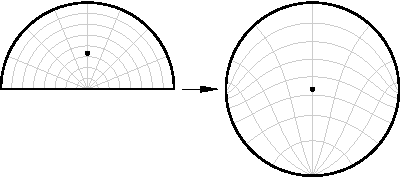
\includegraphics{figures/riemannmap}
\caption{The Riemann map for the upper half-disc with $p=(\sqrt{2}-1)i$.%
\label{fig:riemannmap}}
\end{myfig}

The proof of the theorem is a wonderful example of solving
a problem by formulating a related extremal problem.  The $f$
in the theorem maximizes
$\sabs{f'(p)}$ among injective holomorphic maps taking $p$ to 0.
We will prove that maximizing $\sabs{f'(p)}$ is equivalent to $f$ being
onto:
For any map that is not onto, we find one with a bigger
$\sabs{f'(p)}$ that still goes into the disc.  Such maps are bounded,
so Montel gives us a convergent sequence with $\sabs{f'(p)}$
going to the supremum, and the limit then has to be onto.
Why would one think of this extremal problem?  Well,
maximizing the derivative seems like a good way to spread out the values.
We wish to make the image as large as possible, and we get furthest if the
velocity is largest, no?

\begin{proof}
Consider $\sF$ to be the family of injective (univalent) holomorphic
$f \colon U \to \D$ such that $f(p) = 0$.  We're trying to find
an $f \in \sF$ that is onto.
Before we rush off to Montel, however, we must show that some
injective
$f \colon U \to \D$ actually exists,
that is, that $\sF$ is not empty.  This is where we
use that $U$ is not equal to the complex plane (by Liouville, $\sF$
would be empty if $U = \C$).  If the complement of $U$ contained an open
set, things would be easy, but we can only use that the complement of $U$
contains at least one point, and that $U$ is simply connected.  We will use
the simply-connectedness to construct a square root, as a square root squishes
things together.

Suppose $q \in \C \setminus U$.  The function $z \mapsto z-q$ is never
zero and $U$ is simply connected, so $z-q$ has a holomorphic square
root---there exists a $g \colon U \to \C$ such that
${\bigl(g(z)\bigr)}^2 = z-q$.
The set $g(U)$ is open by the \hyperref[thm:OMT]{open mapping theorem}.
If $g(z)=g(\zeta)$, then ${\bigl(g(z)\bigr)}^2={\bigl(g(\zeta)\bigr)}^2$ and so
$z=\zeta$.  Thus $g$ is injective.  What's more,
$g(z)=-g(\zeta)$ also implies $z=\zeta$.  Thus, $g(z) =
-g(\zeta)$ never happens since $g$ is never zero.
In other words, $g(U) \cap \bigl( - g(U) \bigr) = \emptyset$.  The set
$- g(U)$ (the set of negatives of all points in $g(U)$) is also open, and so
the complement of $g(U)$ contains an open disc $\Delta_r(\xi)$.  Hence,
\begin{equation*}
z \mapsto \frac{r}{g(z)-\xi}
\end{equation*}
takes $U$ to $\D$ and is injective.
By composing with the correct automorphism of the disc,
we find a map that takes $p$ to $0$.  Hence, $\sF$ is nonempty.

OK.  Now suppose that $f \colon U \to \D$ is an injective holomorphic map
such that $f(p) = 0$, but that $f$ is not onto.  There is a
$q \in \D \setminus f(U)$.
Recall that
$\varphi_q(z) = \frac{z-q}{1-\bar{q}z}$ is an automorphism of $\D$ that
takes $q$ to $0$, and consider $\varphi_q \circ f$.  This function is not
zero on $U$ and thus
there exists a holomorphic square root $g$ on $U$, that is,
${\bigl(g(z)\bigr)}^2 = \varphi_q\bigl(f(z)\bigr)$.
The square root of a number in $\D$ is still in $\D$, so $g$
takes $U$ to $\D$.
If $g(z)=g(\zeta)$, then $f(z)=f(\zeta)$ and as
$f$ is injective, $z=\zeta$.  So $g$ is injective.  
The function $g$ takes $p$ to one of the roots of $-q$.
Define
\begin{equation*}
h = \varphi_{g(p)} \circ g .
\end{equation*}
In particular, $h(p) = 0$, and $h \in \sF$.
The inverse of $\varphi_a$ is $\varphi_{-a}$, so
$g = \varphi_{-g(p)} \circ h$.
Next, differentiate
$\varphi_q \circ f = g^2$ at $p$, noting that
and $\varphi_a'(0) = 1-\sabs{a}^2$:
\begin{multline*}
\bigl(1-\sabs{q}^2\bigr) f'(p)
= \varphi_q'\bigl(f(p)\bigr) f'(p)
= 2 g(p) g'(p)
\\
= 2 \varphi_{-g(p)} (0) \varphi_{-g(p)}'(0) h'(p)
= 2 g(p) \bigl(1-\sabs{g(p)}^2\bigr) h'(p) .
\end{multline*}
As ${\bigl(g(p)\bigr)}^2 = -q$, then
\begin{equation*}
\sabs{f'(p)} =
\frac{2 \sabs{g(p)} \bigl(1-\sabs{g(p)}^2\bigr)}{1-\sabs{q}^2} \sabs{h'(p)}
=
\frac{2 \sqrt{\sabs{q}}}{1+\sabs{q}} \sabs{h'(p)}
\end{equation*}
If $\sabs{q} < 1$, then $\frac{2 \sqrt{\sabs{q}}}{1+\sabs{q}} < 1$
(calculus exercise).
In other words,
\begin{equation*}
\sabs{f'(p)} < \sabs{h'(p)} .
\end{equation*}

Take a sequence $\{ f_n \}$ in
$\sF$ such that
\begin{equation*}
\lim_{n \to \infty} \sabs{f_n'(p)} = \sup_{f \in \sF} \sabs{f'(p)}
\end{equation*}
As all functions in $\sF$ are bounded by $1$,
Montel says that there exists a subsequence that converges uniformly on
compact sets to some $f$.  Assume $\{ f_n \}$ is that subsequence.
By the corollary to Hurwitz,
\corref{cor:univalentlimit},
the function $f$ is injective or constant.  It clearly cannot be constant,
as we know that $f_n'(p)$ also converges (all derivatives do), and so it
cannot be zero as 
$\bigl\{ \sabs{f_n'(p)} \bigr\}$ is an increasing sequence.
We must have $f(p) = 0$ by taking the limit.
Similarly 
$\sabs{f(z)} \leq 1$ for all $z \in U$ by taking limits,
so $f(U) \subset \overline{\D}$.
By the \hyperref[thm:OMT]{open mapping theorem}, $f(U) \subset \D$, so $f \in
\sF$.  If $f$ was not onto, then it would not be the one that achieves the
supremum of $\sabs{f'(p)}$.  Thus $f(U) = \D$, and $f$ is the desired map.

The uniqueness is left as an exercise.
\end{proof}

\begin{exbox}
\begin{exercise}
Finish the proof of the theorem:
Given an open $U \subset \C$ and $p \in U$, prove
that a biholomorphic 
$f \colon U \to \D$ such that $f(p) = 0$ and $f'(p) > 0$ is unique if it exists.
\end{exercise}
\end{exbox}

\begin{remark}
The map from the theorem can be useful, but of course the theorem
itself doesn't tell you how to construct it.
There are entire books
written on the subject, collecting the techniques for constructing
these maps for various types of domains.
For instance, there is an explicit formula for the map given any polygon
called the Schwarz--Christoffel mapping.
Let us not worry about these constructions here.
\end{remark}


\begin{remark}
Another interesting question we will not address
is the boundary regularity of the map.  That is, does the map extend to
the closure $\widebar{U}$, and how \myquote{nice} it is.  If $U$ is
bounded by a Jordan curve, it is known that $f$ extends to be continuous on
$\widebar{U}$.  If $U$ has smooth boundary (locally a graph of a smooth
function), then $f$ extends smoothly to $\widebar{U}$.
If $U$ has real-analytic boundary (locally a graph of a real-analytic
function), then $f$ extends holomorphically a bit past the boundary.
Again, we refer the reader to more advanced literature.
\end{remark}

\begin{exbox}
\begin{exercise} \label{exercise:explicitriemann}
Find the unique biholomorphic map (the Riemann map)
$f \colon U \to \D$ explicitly
for the following $U$ and $p$, that is,
such that $f(p) = 0$ and $f'(p) > 0$:
\begin{exparts}
\item
The strip $U = \{ z : -1 < \Im z < 1 \}$, $p=0$.
\item
The quadrant $U = \{ z : \Re z > 0 \text{ and } \Im z > 0 \}$,
$p=\frac{1+i}{\sqrt{2}}$.
\item
The upper half-disc $U = \{ z : \sabs{z} < 1 \text{ and } \Im z > 1 \}$, $p
= (\sqrt{2}-1)i$.  Hint:  Start with the inverse of the Cayley map, and
don't worry about $p$ at first.  See \figureref{fig:riemannmap}.
\end{exparts}
\end{exercise}

\begin{exercise}
Suppose $V \subset \C$ is a simply connected domain, and $V \not= \C$.
Show that every holomorphic $f \colon \C \to V$ is constant.
\end{exercise}

\begin{exercise}
Suppose $U \subset \C$ is a simply connected domain.
Show that for every two points $z,w \in U$, there exists an automorphism
$\psi \in \Aut(U)$ such that $\psi(z) = w$.
\end{exercise}


\begin{exercise}
\begin{exparts}
\item
Suppose $U \subset \C$ is a simply connected domain, $U \not= \C$,
$p,q \in U$ are distinct points, and
$f \colon U \to U$ is holomorphic such that $f(p) = p$ and $f(q)=q$.
Prove that $f$ is the identity, that is, $f(z)=z$ for all $z \in U$.
\item
Find a counterexample if $U=\C$.
\end{exparts}
\end{exercise}

\begin{exercise}
A Riemann-mapping-like theorem for multiply connected domains (domains with
holes) is not true
(at least not in the most obvious way):
Show that the punctured disc $\ann(0;0,1) = \D \setminus \{ 0 \}$
and the annulus $\ann(0;1,2)$ are not biholomorphic.
\end{exercise}

\begin{exercise}
Suppose $U \subset \C$ is a domain.  Suppose one connected component of $\C_\infty
\setminus U$ is more than one point.
\begin{exparts}
\item
Prove that $U$ is biholomorphic to a subset of $\D$.
\item
If $\C_\infty \setminus U$ has finitely many connected components, then
$U$ is biholomorphic to $\D \setminus K$ for some (possibly empty) compact set
$K \subset \D$, where $K$ has finitely many components.
\end{exparts}
Hint: What if the component contained $\infty$?
\end{exercise}

\begin{exercise}
Let $S \subset \C$ be a countable closed subset.
Prove that $U = \C \setminus S$ is not biholomorphic
to any subset of $\D$.  Hint: A countable closed contains isolated points
since every nonempty perfect set is uncountable
(feel free to assume this fact).
\end{exercise}
\end{exbox}

\subsection{Simply connected is simply connected \texorpdfstring{$\star$}{*}}

Let us finally prove that simply connected (in the sense of homology,
\defnref{defn:simplyconnected:homology} that we have been using all this
time), is equivalent to simply connected in the sense of homotopy.
The proof of this corollary is a wonderful example of something that would
be quite difficult without the
\hyperref[thm:RMT]{Riemann mapping theorem}, and it is almost
trivial with the mapping theorem.

\begin{cor} \label{cor:simplyconnhard}
A domain $U \subset \C$ is simply connected in the sense of homotopy
if and only if
it is simply connected in the sense of \defnref{defn:simplyconnected:homology}.
\end{cor}

The key idea is that any path is trivially homotopic to the zero path in the
disc just by scaling.  See also \exampleref{example:homotopydiscsc}.

\begin{proof}
\propref{prop:simplyconneasy} says that if $U$ is
simply connected in the sense of homotopy, then $U$ is simply connected
in the sense of homology.  So let us prove the converse.

Suppose $U$ is simply connected in
the sense of homology.
Let $\gamma \colon [a,b] \to U$ be a continuous function with
$\gamma(a)=\gamma(b)$.  We wish to show that $\gamma$ is homotopic to a
constant in $U$.
The Riemann mapping theorem says that either $U =
\C$ or there is a biholomorphism $f \colon U \to \D$.

If $U = \C$, then define the homotopy $H \colon [a,b] \times [0,1] \to
\C$ as
\begin{equation*}
H(t,s) = (1-s) \gamma(t) .
\end{equation*}
If $U \not= \C$, define $H \colon [a,b] \times [0,1] \to U$ as
\begin{equation*}
H(t,s) = f^{-1} \Bigl( (1-s) f \bigl( \gamma(t) \bigr) \Bigr) .
\end{equation*}
In other words, we map $U$ to $\D$ and consider $f \circ \gamma$.
Then we define $H$ in the same way as we did for $\C$, and then we
take the whole thing back to $U$.
\end{proof}

\begin{remark}
Let us again emphasize that the definition
\myquote{simply connected in terms of homology} is not standard.
It is just a shortcut we took in case we wanted
to skip homotopy on first reading.  In the wild (outside of this book),
\myquote{simply connected} is
always in terms of homotopy.  Furthermore, while for domains in $\C$ the two
concepts happen to be the same, they are not the same for more
general topological spaces.
\end{remark}

\begin{exbox}
\begin{exercise}
Without using the Riemann mapping theorem, \corref{cor:simplyconnhard},
or mapping to the disc in any way, prove by constructing an explicit homotopy
that the slit plane $\C \setminus (-\infty,0]$ is simply connected in
the sense of homotopy, see the proof of the corollary.
\end{exercise}
\end{exbox}

\subsection{Cycles around compacts and simply-connectedness}\label{subsec:patharoundK}

As a second and perhaps much less obvious application of the Riemann
mapping theorem,
we will prove a lemma that around any compact set in some domain $U$
we can find a cycle that goes around this compact set and is homologous to
zero in $U$.
What's interesting is that there is no simply connected domain in sight
in this problem, but we can still use the
\hyperref[thm:RMT]{Riemann mapping theorem}
to greatly
simplify the topology of the situation.
There are more direct and
constructive (but no less technical) ways of proving the lemma below,\footnote{%
The typical proof will put a fine enough square grid on $\C$ and then
show that if we add up all these small cycles whose squares happen to intersect
the compact set and remove the doubled sides, we get the cycle we want.}
but I have an irrational affinity to using the mapping theorem, and this is
my book after all.

This lemma will allow us to finish the proof that simply
connected domains in $\C$ are precisely those 
where the complement in $\C_\infty$ is connected.  That is, we will prove
the converse of \propref{prop:scbycomplementeasy}.  First the lemma.

\begin{lemma}\label{lemma:patharoundK}
Let $U \subset \C$ be open and suppose that $K \subset U$ is compact and
nonempty.
Then there exists a cycle
$\Gamma$ in $U \setminus K$ such that $n(\Gamma;z) = 1$ for all $z \in K$ and
$n(\Gamma;z) = 0$ for all $z \in \C \setminus U$ ($\Gamma$ is homologous to
zero in $U$) and such that $n(\Gamma;z)$ is $0$ or $1$ for all $z \notin
\Gamma$.
\end{lemma}

The intuitive idea of the proof is rather simple.  Suppose $K$ is
connected.
Take one point of it to infinity by an LFT
(an inversion).
Then use the Riemann mapping theorem to make the complement of $K$ go to
the disc (or several discs).
Then the path is a backwards (clockwise) circle very close to the boundary of the disc
as this will \myquote{go around} (after reversing the inversion) what's
\myquote{outside the disc,} that is, it will go around $K$.
The complement of $U$
corresponds to a compact set inside the disc so this way we will not
\myquote{go around} the complement of $U$.
Then one repeat the procedure for all components of $K$.  See
\figureref{fig:cyclearoundcompact}.  As expected,
we hit a bunch of technicalities such as $K$ possibly having
infinitely many connected components, that the complement of a connected
$K$ can have multiple components, and of course that vague intuitive ideas are
nice, but we need to actually do some grubby computation to prove anything.

\begin{myfig}
\subimport*{figures/}{cyclearoundcompact.pdf_t}
\caption{The idea of the proof: The complement of $K$ with infinity goes to
the inside of the disc by Riemann mapping theorem.  The inversion is the
$\varphi$ and $\psi$ is the mapping from Riemann's theorem.
The outside of the disc on the right is not really the image of $K$, but
morally one could think of it that way (hence the quotes).\label{fig:cyclearoundcompact}}
\end{myfig}

\begin{proof}
We first enlarge $K$ so that it
has only finitely many components.  For a small enough $r > 0$, we cover
$K$ by finitely many discs $\Delta_r(z)$ such that $\overline{\Delta_r(z)}
\subset U$.  In particular, for some $z_1,\ldots,z_n$,
\begin{equation*}
K' =
\overline{\Delta_r(z_1)}
\cup \cdots \cup
\overline{\Delta_r(z_n)}
\end{equation*}
is a compact subset of $U$ and $K \subset K'$.
As $K'$ is a union of finitely many closed discs, it has
finitely many topological components.
If we find a $\Gamma$ in $U$ around $K'$, then we are done as $K \subset K'$.

Let $K_1,\ldots,K_n$ be the components of $K'$.
The components are closed, and as there are finitely many,
$K_2 \cup \cdots \cup K_n$ is also closed.
If we prove the lemma for the connected compact set $K_1$ and
the open set $U \setminus ( K_2 \cup \cdots \cup K_n )$ to find a cycle
$\Gamma_1$, then we claim we are done: We could repeat the procedure
for each $K_j$ to find $\Gamma_j$ and let $\Gamma = \Gamma_1 + \cdots +
\Gamma_n$.  As $\Gamma_j$ winds exactly once around every point of $K_j$
and does not wind around any point of $K_\ell$ for $\ell \not= j$,
then $\Gamma$ will wind exactly once around any point of $K'$,
and it still homologous to zero in $U$.

So, without loss of generality, assume that $K$ is connected.
Also assume that $0 \in K$.  If $K= \{0 \}$, we are done trivially, so
assume $K$ is larger than one point.
Consider $\varphi \colon \C_\infty \to \C_\infty$ be the inversion
LFT:
$\varphi(z) = \nicefrac{1}{z}$ for $z \in \C \setminus \{ 0 \}$,
$\varphi(0) = \infty$ and $\varphi(\infty) = 0$.
Being an LFT, $\varphi$ is a (bi)holomorphic
mapping of $\C_\infty$ to itself, where $\varphi^{-1} = \varphi$.  Let
\begin{equation*}
V = \varphi(\C_\infty \setminus K) .
\end{equation*}
Note that $\infty \notin V$, $0 \in V$, $V \not= \C$ ($K$ is more than one
point), and
$\C_\infty \setminus V = \varphi(K)$ is connected.
So each connected component of $V$ is a simply connected domain
by \propref{prop:scbycomplementeasy} (exercise).
As we can assume that $K$ is a finite union of closed discs,
$\C_\infty \setminus K$ and therefore $V$ has finitely many connected components.
Let $V_1,\ldots,V_m$ be the connected
components of $V$.
By the Riemann mapping theorem, there exists
a biholomorphic map from $V_j$ to $\Delta_1(q_j)$,
where $q_1,\ldots,q_m$ are some points
far enough apart so that the discs are disjoint.
Write $D = \Delta_1(q_1) \cup \cdots \cup \Delta_1(q_m)$.
In other words, there is
a biholomorphic $\psi \colon V \to D$.  We can arrange that $q_1=0$
and $\psi(0)=0$.

The set $\C_\infty \setminus U$ is compact: It is a closed subset of
a compact set $\C_\infty$.  As $\varphi$ is continuous,
$\varphi(\C_\infty \setminus U)$ is compact, and a subset of $V$.
And as $\psi$ is continuous,
\begin{equation*}
S = \psi\bigl(\varphi(\C_\infty \setminus U)\bigr)
\end{equation*}
is a compact subset of $D$.  There is an $r < 1$ such that
\begin{equation*}
S \subset \Delta_r(q_1) \cup \cdots \cup \Delta_r(q_m) .
\end{equation*}
Consider the paths $\gamma_j(t) = q_j + r e^{-it}$ for $t \in
[0,2\pi]$,
that is, $\gamma_j = -\partial
\Delta_r(q_j)$.
Let $\Gamma_j=\varphi^{-1} \circ \psi^{-1} \circ \gamma_j$, and $\Gamma = \Gamma_1 +
\cdots + \Gamma_m$.

Let us compute the winding numbers.
For any $p$ not on $\Gamma$ compute
the winding number (see \propref{prop:usubst}):
\begin{multline*}
n(\Gamma;p) = 
\sum_{j=1}^m
\frac{1}{2\pi i}
\int_{\varphi^{-1} \circ \psi^{-1} \circ \gamma_j}
\frac{1}{z-p} \, dz
=
\sum_{j=1}^m
\frac{1}{2\pi i}
\int_{\psi^{-1} \circ \gamma_j}
\frac{-1}{(1-\zeta p) \zeta} \, d\zeta
\\
=
\sum_{j=1}^m
\frac{1}{2\pi i}
\int_{\gamma_j}
\frac{-1}{ \bigl( 1-\psi^{-1}(\xi)p \bigr)
\,
\psi^{-1}(\xi)
\,
\psi' \bigl(\psi^{-1}(\xi)\bigr)} \, d \xi .
\end{multline*}

First suppose that $p \in \C \setminus U$.
The function 
\begin{equation*}
h(\xi) =
\frac{-1}{ \bigl( 1-\psi^{-1}(\xi)p \bigr)
\,
\psi^{-1}(\xi)
\,
\psi' \bigl(\psi^{-1}(\xi)\bigr)}
\end{equation*}
defined on $D$ has two poles: one at $\psi(\nicefrac{1}{p})$ and one
at $q_1=0$ (the third factor in the denominator is never zero).
They are both simple poles as is easy to check and the residues are (using
\propref{prop:residuesimpleratio})
\begin{equation*}
\operatorname{Res}(h;0) = 
\frac{-1}{ \bigl( 1-\psi^{-1}(0)p \bigr)
\,
\psi' \bigl(\psi^{-1}(0)\bigr)}
\,
\frac{1}{\frac{1}{\psi'(\psi^{-1}(0))}}
=
-1
\end{equation*}
and
\begin{equation*}
\operatorname{Res}\bigl(h;\psi(\nicefrac{1}{p})\bigr)
=
\frac{-1}{
\psi^{-1}\bigl(\psi(\nicefrac{1}{p})\bigr)
\,
\psi' \bigl(\psi^{-1}(\psi(\nicefrac{1}{p}))\bigr)
}
\,
\frac{1}{
\frac{-1}{\psi'(\psi^{-1}(\psi(1/p)))}
\, p
}
=
1 .
\end{equation*}
The path $\gamma_1$ goes around $q_1=0$.
Some $\gamma_j$ goes around
$\psi(\nicefrac{1}{p})$, as $r$ was picked sufficiently large
precisely so that the circles $\gamma_j$ go around $S$, that is points that
are the image of $\C \setminus U$,
in particular $\psi(\nicefrac{1}{p})$.
The sum of the residues which is zero, so 
by the \hyperref[thm:residue]{residue theorem},
\begin{equation*}
n(\Gamma;p) = 0 .
\end{equation*}

Next suppose $p \in K$.  As before
$n(\Gamma;p) = 
\sum_j
\frac{1}{2\pi i}
\int_{\gamma_j} h(\xi) \, d\xi$.
As $p \in K$, $\psi^{-1}(\xi) \not= p$ for all $\xi \in D$,
and so $h$ has just the pole at $0$.
Since $\gamma_1$ traverses the circle backwards,
\begin{equation*}
n(\Gamma;p) = 
\sum_{j=1}^m
\frac{1}{2\pi i}
\int_{\gamma_j} h(\xi) \, d\xi 
=
\frac{1}{2\pi i}
\int_{\gamma_1} h(\xi) \, d\xi 
= - \operatorname{Res}(h;0) = 1 .
\end{equation*}

If $p$ is any other point not on $\Gamma$, then $n(\Gamma;p)$
is either $0$ or $1$, depending on if there is a pole at
$\psi(\nicefrac{1}{p})$ and if $\Gamma$ goes around it or not.
\end{proof}

\begin{exbox}
\begin{exercise}
Prove that if $K \subset \C_\infty$ is compact and connected, then 
every component of $\C_\infty \setminus K$ is a simply connected domain.
Hint: Prove that the complement of each one of these components is connected.
\end{exercise}
\end{exbox}

We can now prove the simplest
topological characterization of simply connected domains in $\C$.

\begin{thm} \label{cor:scbycomplementhard}
Let $U \subset \C$ be a domain.  Then
$\C_\infty \setminus U$ is connected if and only if $U$ is simply connected.
\end{thm}

\begin{proof}
The forward direction is \propref{prop:scbycomplementeasy}.  Let's the do
the backwards direction by contrapositive.  Suppose $\C_\infty
\setminus U$ is disconnected.  Then there are two nonempty disjoint closed
sets $S$ and $K$ such that $S \cup K = \C_\infty \setminus U$. 
Assume $\infty \in S$.
The set $U' = U \cup K$ is open as $S$ is closed, $U' \subset \C$,
and $K \subset U'$ is compact.  Apply the lemma to find a cycle
$\Gamma$ in $U = U' \setminus K$ such that $n(\Gamma;z) = 1$ for all $z \in
K$.  In other words, $\Gamma$ is not homologous to zero in $U$.
\end{proof}

\begin{exbox}
\begin{exercise}
Suppose $K \subset \C$ is compact and connected, $\C \setminus K$ is
connected, and $K$ is more than one point.
Prove that there exists a biholomorphic
map $\psi \colon \C \setminus K \to \C \setminus \overline{\D}$.
\end{exercise}

\begin{exercise}
Construct an example compact set $K \subset \C$ with a connected component $K_1$
with the following property.
For every cycle $\Gamma$ in $\C \setminus K$ such that $n(\Gamma;z)=1$ for
all $z \in K_1$,
there exists a $\zeta \in K \setminus K_1$ where $n(\Gamma;\zeta)=1$.
Why does this not contradict the construction in the proof of the lemma?
\end{exercise}

\begin{exercise}
Suppose $\{ f_n \}$ is a sequence of holomorphic functions on an open set
$U \subset \C$ that converges uniformly on compact subsets to
$f \colon U \to \C$.  Let $K \subset U$ be a compact set.  Prove that
for every open neighborhood $V$ of $K$ in $U$ (so $K \subset V \subset U$) there exists
a smaller open neighborhood $W$ (so $K \subset W \subset V$) and an $N \in \N$
such that $f$ and $f_n$ have the same number of zeros in $W$ for all
$n \geq N$.
\end{exercise}

\begin{exercise}
Given an open $U \subset \C$, a compact nonempty $K \subset U$, and a $\delta > 0$,
prove there
exists a cycle $\Gamma$ in $U \setminus K$ homologous to zero in $U$,
such that $n(\Gamma;z)$ is either $0$ or $1$ for all $z \notin \Gamma$,
such that
$n(\Gamma;z) = 1$ for all $z \in K$, 
and such that for every $p \in \Gamma$ there is a $q \in K$ such that
$\sabs{p-q} < \delta$ ($\Gamma$ is within $\delta$ of $K$).
\end{exercise}
\end{exbox}

%%%%%%%%%%%%%%%%%%%%%%%%%%%%%%%%%%%%%%%%%%%%%%%%%%%%%%%%%%%%%%%%%%%%%%%%%%%%%%
%%%%%%%%%%%%%%%%%%%%%%%%%%%%%%%%%%%%%%%%%%%%%%%%%%%%%%%%%%%%%%%%%%%%%%%%%%%%%%
%%%%%%%%%%%%%%%%%%%%%%%%%%%%%%%%%%%%%%%%%%%%%%%%%%%%%%%%%%%%%%%%%%%%%%%%%%%%%%

\chapter{Harmonic Functions} \label{ch:harmonic}

\begin{myepigraph}
If you cannot get rid of the family skeleton, you may as well make it
dance.

---George Bernard Shaw
\end{myepigraph}

%%%%%%%%%%%%%%%%%%%%%%%%%%%%%%%%%%%%%%%%%%%%%%%%%%%%%%%%%%%%%%%%%%%%%%%%%%%%%%

\section{Harmonic functions}
\label{sec:harmonic}

Hitherto, we examined holomorphic functions as complex-valued functions.
However, to do analysis one needs inequalities, and complex numbers are not
ordered.  Let us consider the real and imaginary parts of holomorphic
functions, the so-called harmonic functions.  Interestingly, harmonic
functions come up often in applied mathematics, for example as steady state
heat or the distribution of electrostatic potential in a region without
charge.  Harmonic functions are used to study
holomorphic functions and vice versa, holomorphic functions are used to
study harmonic functions.

Most of the results
we will prove for harmonic functions are analogues of the results 
for holomorphic functions.  The reader is
encouraged to look for these connections.
Just as it is best to study animals in their natural habitat,
many results we proved for holomorphic functions are
better understood as results for harmonic functions.
Nevertheless, the results for harmonic functions are not
always a simple application of what has already been proved for holomorphic
functions, and even the
statements or proofs of the analogous results may be quite different.
Harmonic functions are somewhat more general than real and
imaginary parts of holomorphic functions.  They are real and imaginary parts
of holomorphic functions only locally, but perhaps not globally.


\subsection{Real and imaginary parts of holomorphic functions}

\begin{defn}
Let $U \subset \C$ be open.
A twice continuously (real) differentiable ($C^2$ for short) function $f \colon U \to \R$ is
\emph{\myindex{harmonic}} if
\glsadd{not:laplacian}%
\begin{equation*}
\nabla^2 f =
\frac{\partial^2 f}{\partial x^2} +
\frac{\partial^2 f}{\partial y^2} = 0
\quad \text{ on $U$.}
\end{equation*}
\end{defn}

The operator $\nabla^2$, sometimes written $\Delta$,
is the \emph{\myindex{Laplacian}}.\footnote{%
The Laplacian is defined in $\R^n$ for any $n$ by
$\nabla^2 f =
\frac{\partial^2 f}{\partial x_1^2} + \cdots +
\frac{\partial^2 f}{\partial x_n^2}$, and so there
are harmonic functions in any dimension.
We are interested in the complex plane, $n=2$,
which is surprisingly different from the $n \geq 3$ case.
When $n \geq 3$, the theory has far less to do with complex analysis.}
It is the trace of the Hessian matrix.  It is convenient 
to note that
\begin{equation*}
4
\frac{\partial^2}{\partial \bar{z}\partial z} f =
4
\left[
\frac{1}{2}
\left(
\frac{\partial}{\partial x} + i
\frac{\partial}{\partial y}
\right)
\right]
\left[
\frac{1}{2}
\left(
\frac{\partial}{\partial x} - i
\frac{\partial}{\partial y}
\right)
\right]
f
=
\left[
\frac{\partial^2}{\partial x^2} +
\frac{\partial^2}{\partial y^2}
\right]
f
=
\nabla^2 f .
\end{equation*}

Namely, $f$ is harmonic if and only if
$\frac{\partial f}{\partial z}$ is holomorphic.
Locally (in some neighborhood), we find a
primitive $g$ of $\frac{\partial f}{\partial z}$, and we write
\begin{equation*}
f(z) = g(z) + c(z) ,
\end{equation*}
where $g$ is holomorphic, $c$ is at least $C^2$, and $\frac{\partial c}{\partial z} \equiv 0$.
Let $h = \bar{c}$ be the complex conjugate of $c$.  Then 
\begin{equation*}
\frac{\partial h}{\partial \bar{z}}
=
\frac{\partial \bar{c}}{\partial \bar{z}}
=
\overline{
\frac{\partial c}{\partial z}
}
=
0 ,
\end{equation*}
so $h$ is holomorphic.  Thus, for some holomorphic $g$ and $h$,
\begin{equation*}
f(z) = g(z) + \overline{h(z)} .
\end{equation*}
Consider the holomorphic $\varphi(z) = g(z) + h(z)$.
As $f$ is real-valued,
\begin{equation*}
f(z) = \Re f(z) =
\frac{g(z) + \overline{h(z)} + \overline{g(z)}+h(z)}{2}
=
\frac{g(z) + h(z) + \overline{g(z)+h(z)}}{2}
=
\Re \varphi(z) .
\end{equation*}
So any harmonic function $f$ is locally the real part of a holomorphic
function.  Similarly $f$ is locally the imaginary part of a holomorphic
function.
This all works only in some neighborhood.  We cannot necessarily find a single
$\varphi$ (the $g$ and $h$ above) in the entire
domain $U$, unless $U$ is simply connected.  If not, we can always
pick a simply connected neighborhood, such as a disc.
If $U$ is simply connected, then
$\frac{\partial f}{\partial z}$ has a primitive in $U$,
and the computation above leads to
the following proposition.

\begin{prop} \label{prop:harmconj}
Let $U \subset \C$ be a simply connected domain and $f \colon U \to \R$ a
harmonic function.  Then there exists a holomorphic $\varphi \colon
U \to \C$ such that $f = \Re \varphi$.
\end{prop}

Conversely,
suppose that $f$ is the real-part of a holomorphic function $\varphi$:
\begin{equation*}
f(z) = \Re \varphi(z) =
\frac{1}{2}\bigl( \varphi(z) + \overline{\varphi(z)} \bigr) .
\end{equation*}
Notice that
\begin{equation*}
\nabla^2 =
4 \frac{\partial^2}{\partial \bar{z} \partial z}
=
4 \frac{\partial^2}{\partial z \partial \bar{z}} .
\end{equation*}
Then
\begin{equation*}
\nabla^2 f =
4 \frac{\partial^2}{\partial \bar{z} \partial z}
\left(
\frac{1}{2}\bigl( \varphi(z) + \overline{\varphi(z)} \bigr)
\right)
=
2
\left(
\frac{\partial}{\partial z}
\left(
\frac{\partial}{\partial \bar{z}}
\varphi(z)
\right)+
\frac{\partial}{\partial \bar{z}}
\left(
\frac{\partial}{\partial z}
\overline{\varphi(z)}
\right)
\right)
=
0 .
\end{equation*}
We have thus proved the following characterization of harmonic
functions.

\begin{prop} \label{prop:harmanal}
Let $U \subset \C$ be open and $f \colon U \to \R$ a function.
\begin{enumerate}[(i)]
\item
The function $f$ is harmonic if and only if
for every point $p \in U$ there exists an open neighborhood $V$ of $p$ and a
holomorphic $\varphi \colon V \to \C$ such that $f = \Re \varphi$
on $V$.
\item
The function $f$ is harmonic if and only if
for every $p \in U$, there exists a power series expansion
\begin{equation*}
f(z) =
c_0
+
\sum_{n=1}^\infty c_n {(z-p)}^n + \bar{c}_n {\overline{(z-p)}}^n
\end{equation*}
converging uniformly absolutely
on every closed disc $\overline{\Delta_r(p)} \subset U$.
\end{enumerate}
\end{prop}

As holomorphic functions are
infinitely differentiable, harmonic functions are as well.
Actually, we see above that harmonic functions have a real power series
(a power series in $x$ and $y$, or equivalently in $z$ and $\bar{z}$)
and so they are what is called real-analytic.

\begin{prop}
If $U \subset \C$ is open and $f \colon U \to \R$ is harmonic, then $f$ is infinitely (real) differentiable.
\end{prop}

Starting with a harmonic function $f$, finding the holomorphic function whose
real part is $f$ means finding another harmonic function such that $f+ig$ is
holomorphic.

\begin{defn}
Let $U \subset \C$ be open and $f \colon U \to \R$ harmonic.
If $g \colon U \to \R$ is harmonic and $f + i g$ is holomorphic,
then $g$ is called the \emph{\myindex{harmonic conjugate}} of $f$.
\end{defn}

\propref{prop:harmconj}
says that every harmonic function on a simply connected
domain has a harmonic conjugate.  On the other hand, on the punctured plane
$\C \setminus \{ 0 \}$, the harmonic function $\log \sabs{z}$ 
fails to have a harmonic conjugate.  If it did have a harmonic conjugate,
then $\log$ would have a branch in $\C \setminus \{0\}$, which it does not.
See \figureref{fig:loggraph}, the graph of the real part on the left is
continuous, but the corresponding imaginary part is not a function.
That we cannot find a different conjugate for $\log \sabs{z}$
follows from the following proposition.

\begin{prop} \label{prop:harmonicconjdifferbyconst}
If $U \subset \C$ is a domain $f \colon U \to \R$ is harmonic
and $g_1$ and $g_2$ are two harmonic conjugates of $f$,
then $g_1 = g_2 + C$ for some $C \in \R$.
\end{prop}

The proof is trivial: The hypothesis implies that
\begin{equation*}
\frac{(f + i g_1) - (f + i g_2)}{i} =  g_1-g_2
\end{equation*}
is holomorphic and it is real-valued on $U$, and thus constant.

The real and imaginary parts of a holomorphic function are harmonic;
however, the modulus $\sabs{f(z)}$ is not.  Not to fear,
$\log \sabs{f(z)}$ is harmonic, at least where $f$ is nonzero.
The fact that $\log \sabs{f(z)}$ is harmonic is just as useful
as that the real and imaginary parts of $f$ are.  The proof is left
as an exercise.

\begin{prop} \label{prop:logharm}
Suppose $U \subset \C$ is open, $f \colon U \to \C$ is holomorphic
and never zero.  Then
\begin{equation*}
z \mapsto \log \sabs{f(z)}
\end{equation*}
is harmonic.
\end{prop}

\begin{savenotes}
\begin{exbox}
\begin{exercise}
Prove \propref{prop:logharm}.
\end{exercise}

\begin{exercise}
Show that the following functions of $x$ and $y$ (where
$z = x+iy$) are
harmonic (either on $\C$ or on the set given)
and find their harmonic conjugate.
\smallskip
\begin{expartshor}{5}
\item
$y$
\item
$xy$
\item
$\arctan(y/x)$ on $x \not= 0$
\item
$\frac{x}{x^2+y^2}$ on $z\not=0$
\end{expartshor}
\end{exercise}

\begin{exercise}
Suppose that $U \subset \C$ is a simply connected domain
and $f \colon U \to \R$ a harmonic function.  Prove that there exists
a holomorphic function $\varphi \colon U \to \C$ such that
$f(z) = \log \sabs{\varphi(z)}$.
\end{exercise}

\begin{exercise}
Let $U,V \subset \C$ be open sets and
$f \colon U \to V$ be holomorphic. Prove:
\begin{exparts}
\item
If $g \colon V \to \R$ is harmonic, then
$g \circ f$ is harmonic.
\item
Let $f$ be a biholomorphism of $U$ and $V$.
Then $g \colon V \to \R$ is harmonic if and only if
$g \circ f$ is harmonic.
\end{exparts}
\end{exercise}

\begin{exercise}
Prove that if $f \colon \D \to \R$ is harmonic, then
$f(\nicefrac{z}{\sabs{z}^2})$ is harmonic in $\C \setminus
\overline{\D}$.
\end{exercise}

\begin{exercise}
Suppose $U \subset \C$ is a domain and
$f \colon U \to \C$ is holomorphic.  Prove that
if $z \mapsto \sabs{f(z)}^2$ is harmonic, then $f$ is constant.
\end{exercise}

\begin{exercise}
Suppose $f \colon \C \to \R$ is harmonic.
\begin{exparts}
\item
Show that there exists
a holomorphic $F \colon \C \setminus \{ 0 \} \to \C$
such that $F=f$ on $\partial \D$.
\item
Show that if $F$ from part a) has a pole at the origin, then $f$
is the real part of a holomorphic polynomial.
\end{exparts}
\end{exercise}

\begin{exercise}
Suppose $U \subset \C$ is open, $\overline{\D} \subset U$,
and $f \colon U \to \R$ is harmonic.  Expand
$f$ as a real power series at the origin as in \propref{prop:harmanal}, and find a formula
for the $c_n$ in terms
of an integral around $\partial \D$.
\end{exercise}

% Best for this to be the last in this exbox,
% so that the footnote (due to the savenotes) appears
% (most likely) on the right page.
\begin{exercise}\label{exercise:Liouvilleharmonic}
\pagebreak[2]
Prove the Liouville\footnote{%
See
Nelson, Edward
\emph{A proof of Liouville's theorem.}
Proc.\ Amer.\ Math.\ Soc.\ {\textbf{12}} (1961), 995
(one of the shortest published papers) for
an elegant proof for bounded functions.
But you can't use it, you don't have the
tools for it yet.} theorem\index{Liouville theorem!harmonic functions} for
harmonic functions:  If $f \colon \C \to \R$ is harmonic
and nonnegative, then $f$ is constant.
\end{exercise}
\end{exbox}
\end{savenotes}

\begin{remark}
As in \exerciseref{exercise:Liouvilleharmonic},
the analogue of \myquote{bounded} for holomorphic functions is
\myquote{nonnegative}
for harmonic functions.  Afterall, if $f$ is
a bounded holomorphic function, then $\log \sabs{f(z)+M}$ or $\Re f(z) + M$
is nonnegative for large enough $M$.  Conversely if $\log \sabs{f(z)} \geq
0$, then $\frac{1}{f(z)}$ is bounded, and if $\Re f(z) \geq 0$, then
$\frac{f(z)-1}{f(z)+1}$ is bounded (composing $f$ with an LFT taking the
right half-plane to the disc).
\end{remark}


\begin{remark}
The procedure above, writing
\begin{equation*}
\frac{\partial^2}{\partial x^2}+ \frac{\partial^2}{\partial y^2} = 
4 \frac{\partial^2}{\partial \bar{z} \partial z} ,
\end{equation*}
that is, a sum of derivatives as a composition of
different derivatives,
so that we could integrate in these two new variables, may
sound familiar.  In this case we obtained a harmonic $f$ as a function
of $z$ (a holomorphic function) plus a function of $\bar{z}$ (an
antiholomorphic function).

The procedure is analogous to the D'Alembert solution of the one-dimensional
wave equation you may have seen in undergraduate differential equations.
The wave operator is
$\frac{\partial^2}{\partial t^2}- \frac{\partial^2}{\partial x^2}$ with a
minus sign, and we use $x$ and $t$ as variables to be traditional.
The wave operator decomposes as
\begin{equation*}
\frac{\partial^2}{\partial t^2}- \frac{\partial^2}{\partial x^2}
=
\left[ \frac{\partial}{\partial t}- \frac{\partial}{\partial x}
\right]
\left[ \frac{\partial}{\partial t}+ \frac{\partial}{\partial x}
\right] .
\end{equation*}
So if we write $\mu = x+t$ and $\eta = x-t$ (the so-called characteristic
variables), then
\begin{equation*}
-4 \frac{\partial^2}{\partial \eta \partial \mu} = 
\frac{\partial^2}{\partial t^2}- \frac{\partial^2}{\partial x^2} .
\end{equation*}
As before, a solution $f$ to the wave equation is a function
of $\mu$ plus a function of $\eta$.  That is, $f(x,t) = A(\mu) + B(\eta) =
A(x+t)+B(x-t)$, two waves travelling in opposite directions.  The
functions $A$ and $B$ need not be nice at all, any twice real differentiable
functions.
It is interesting that one puny minus sign makes such a huge difference.
\end{remark}

\subsection{Identity and the maximum principle}

A consequence of the propositions above is the identity theorem
for harmonic functions.
The zero set of a harmonic function is allowed to have limit points.
For instance, $\Re z$ is zero on the entire imaginary
axis.  However, we are still not allowed open sets for nonconstant harmonic
functions.  It is really a property of real-analytic functions, that is,
functions that have a power series representation in terms of $x$ and $y$
or $z$ and $\bar{z}$, but we do not wish to get far into power series in two
variables.

\begin{thm}[Identity]\index{identity theorem!harmonic functions}
Let $U \subset \C$ be a domain and $f \colon U \to \R$ a harmonic function.
Suppose $V \subset U$ is a nonempty open subset and $f = 0$ on $V$.  Then $f
\equiv 0$.
\end{thm}

\begin{proof}
Let $Z_f$ be the zero set of $f$ and let $Z$ be the closure of the interior
of $Z_f$ in the subspace topology of $U$.
The set $Z$ is nonempty by hypothesis, so
consider some $p \in Z$.  For any disc $\Delta_r(p) \subset U$, $f$ is
zero on some open subset of the disc.  On $\Delta_r(p)$, the function
$f$ has a harmonic
conjugate $g$ and $f+i g$ is a holomorphic function that is purely imaginary on
an open subset of $\Delta_r(p)$ and hence constant on that open subset.
By the \hyperref[thm:identity]{identity theorem for holomorphic functions},
$f+ig$ is constant 
on $\Delta_r(p)$.
Since $f$ is zero somewhere on the
disc and constant, it is zero on the entire disc.  Thus $Z$
is open, $Z$ is also closed, so $Z=U$ as $U$ is connected.
\end{proof}

The maximum principle is really a theorem about harmonic functions rather
than holomorphic functions.  We will prove it using holomorphic functions
and the open mapping theorem (\thmref{thm:OMT})\footnote{%
The open mapping theorem is a stronger version of the maximum modulus principle.}
although there is a more natural proof using the mean value property,
which we will see later.

\begin{thm}[Maximum principle]
\index{maximum principle!harmonic functions}%
Suppose $U \subset \C$ is a domain and $f \colon U \to \R$
is harmonic.  If $f$ attains a local maximum (or a local minimum) in $U$, then $f$ is constant.
\end{thm}

\begin{proof}
Suppose that $f$ attains a local maximum at $p \in U$.
The statement for a minimum follows by considering $-f$.
Let $\Delta_r(p) \subset U$
be a disc such that $p$ is the maximum of $f$ on $\Delta_r(p)$.
There exists a holomorphic $h \colon \Delta_r(p) \to \C$
such that $f = \Re h$.
Then $h$ takes
$\Delta_r(p)$ to a subset of $X = \bigl\{ w \in \C : \Re w \leq f(p) \bigr\}$.
The point $h(p)$ is on the boundary of $X$ as $\Re h(p)= f(p)$.  Hence,
$h\bigl(\Delta_r(p)\bigr)$ is not open, which can only happen if $h$ is
constant by the open mapping theorem.  As $f$ is constant on $\Delta_r(p)$, it is constant on $U$ by the
identity theorem.
\end{proof}

\begin{exbox}
\begin{exercise}
Prove that
the maximum principle for harmonic functions implies the maximum
modulus principle for holomorphic functions.
Hint: Consider $\log \sabs{f(z)}$.
\end{exercise}

\begin{exercise}%[\neededexmark]
\label{exercise:maxprincsecondharmonic}
Prove the second version of the maximum principle: If $U \subset \C$
is a bounded domain and
$f \colon \widebar{U} \to \R$ is continuous and harmonic on $U$,
then $f$ achieves both its maximum and its minimum
on the boundary $\partial U$.
\end{exercise}

\begin{exercise}
Suppose $U \subset \C$ is open such that $\R \cap U \not= \emptyset$
and $\R \cap U$ is connected.
Suppose $f \colon U \to \R$ is harmonic
and the zero set of the restriction $f|_{\R \cap U}$ has a limit point in
$\R \cap U$.  Prove that $f|_{\R \cap U} \equiv 0$.
\end{exercise}

\begin{exercise}
Suppose $U \subset \C$ is a domain and
$f \colon U \to \R$ is harmonic.
Prove that $f(U)$ is an open interval or a single point.
\end{exercise}
\end{exbox}

%%%%%%%%%%%%%%%%%%%%%%%%%%%%%%%%%%%%%%%%%%%%%%%%%%%%%%%%%%%%%%%%%%%%%%%%%%%%%%

\section{The Dirichlet problem in a disc and applications}

\subsection{The Dirichlet problem in a disc and the Poisson kernel}

It is useful to find a harmonic function given boundary values:
Given an open $U \subset \C$
and a continuous $f \colon \partial U \to \R$,
find a continuous $g \colon \widebar{U} \to \R$,
harmonic on $U$, such that $g|_{\partial U} = f$.
This problem is called the \emph{\myindex{Dirichlet problem}}, and it is
solvable for many (though not all) open sets.  If the solution exists on a
bounded domain, then it is unique.  On unbounded domains, the solution need not
be unique, see \exerciseref{exercise:upperhalfplanedirichlet}.

\begin{prop}
Suppose $U \subset \C$ is a bounded domain, $f,g \colon \widebar{U} \to \R$
are continuous functions, harmonic on $U$,
such that $f = g$ on $\partial U$.
Then $f=g$ on $U$.
\end{prop}

\begin{proof}
Apply the maximum principle (second version,
\exerciseref{exercise:maxprincsecondharmonic}) to $f-g$.
\end{proof}

The solution of the problem in a disc is rather useful and rather explicit.
It is achieved by integration against the so-called
\emph{\myindex{Poisson kernel}}.
The
Poisson kernel
for the unit disc $\D \subset \C$,
is
\glsadd{not:Pr}%
\begin{equation*}
P_r(\theta)
= \frac{1}{2\pi} \frac{1-r^2}{1+r^2-2r \cos \theta}
= \frac{1}{2\pi}
\Re \left( \frac{1+re^{i\theta}}{1-re^{i\theta}}\right) ,
\qquad \text{for $0 \leq r < 1$.}
\end{equation*}
As a function of $z \in \D$
the Poisson kernel is (see \figureref{fig:poissongraph})
\begin{equation*}
z \mapsto \frac{1}{2\pi} \Re \left(
\frac{1+z}{1-z}\right).
\end{equation*}
\begin{myfig}
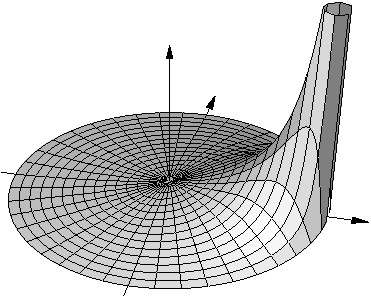
\includegraphics{figures/poisson-graph}
\caption{Graph of the Poisson kernel on $\D$, the pole at $z=1$ is cut off at 2.%
\label{fig:poissongraph}}
\end{myfig}

\begin{prop}\label{prop:Poissonprops}
\leavevmode
\begin{enumerate}[(i)]
\item
$P_r(\theta) > 0$ for all $0 \leq r < 1$ and all $\theta$.
\item
$\int_{-\pi}^{\pi} P_r(\theta) \, d\theta = 1$
for all $0 \leq r < 1$.
\item
For any given $\delta > 0$,
$\sup \bigl\{P_r(\theta) : \delta \leq \abs{\theta} \leq
\pi \bigr\} \to 0$ as $r \uparrow 1$.
\end{enumerate}
\end{prop}

In the proof, it is useful to visualize the graph of
$P_r$ as a function of $\theta$ for a fixed $r$.
See \figureref{fig:poisson2dgraph}.

\begin{myfig}
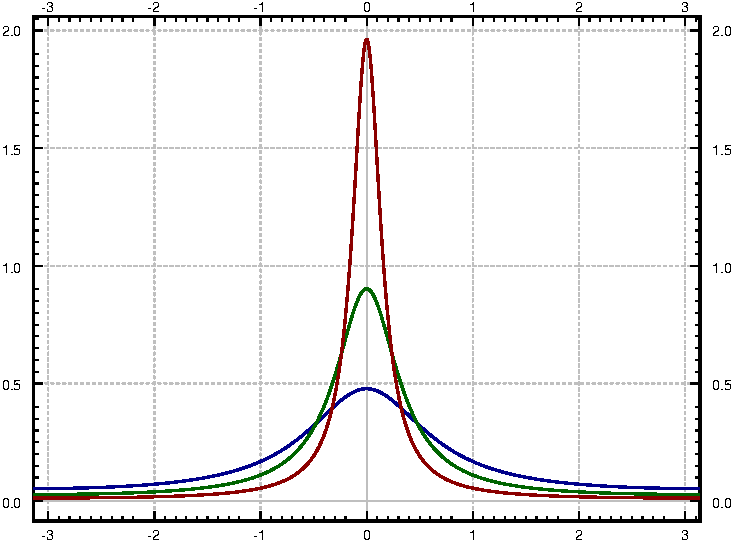
\includegraphics[width=0.5\textwidth]{figures/poisson-kernel.pdf}
\caption{The graph of $P_r$ as a function of $\theta$ on $[-\pi,\pi]$ for
$r=0.5$, $r=0.7$, and $r=0.85$.\label{fig:poisson2dgraph}}
\end{myfig}

\begin{proof}
The first item follows because $1-r^2$ is always positive if $0 \leq r < 1$,
and similarly
\begin{equation*}
1+r^2-2r \cos\theta \geq 1+r^2-2r = {(1-r)}^2 > 0 .
\end{equation*}

For the second item,
\begin{equation*}
\begin{split}
\int_{-\pi}^{\pi}
P_r(\theta) \, d\theta
& =
\frac{1}{2\pi}
\int_{-\pi}^{\pi}
\Re
\left(
\frac{1+re^{i\theta}}{1-re^{i\theta}}
\right)
\, d\theta
\\
& =
\Re
\frac{1}{2\pi i}
\int_{-\pi}^{\pi}
\frac{1+re^{i\theta}}{1-re^{i\theta}} \frac{1}{re^{i\theta}} \,
ire^{i\theta}
\, d\theta
\\
& = 
\Re
\frac{1}{2\pi i}
\int_{\partial \Delta_r(0)}
\frac{(1+z)/(1-z)}{z} \, dz
=
\Re \frac{1+0}{1-0} = 1 .
\end{split}
\end{equation*}
The equality on the third line follows by the Cauchy integral formula
using the function $\frac{1+z}{1-z}$ evaluated at $0$.

For the third item, we only need to prove the
result for $\delta \leq \theta \leq \pi$ by symmetry ($P_r$ is even).
On $(0,\pi)$, $P_r$ is strictly decreasing as $\cos \theta$ is strictly
increasing.  So we only need to show that $P_r(\delta)$ goes to $0$
as $r \to 1$ if $\delta > 0$.
This follows as $r \mapsto
\frac{1+re^{i\delta}}{1-re^{i\delta}}$
is continuous at $r=1$ and
\begin{equation*}
\frac{1+e^{i\delta}}{1-e^{i\delta}}
=
\frac{(1+e^{i\delta})(1-e^{-i\delta})}{(1-e^{i\delta})(1-e^{-i\delta})}
=
\frac{e^{i\delta}-e^{i\delta}}{\sabs{1-e^{i\delta}}^2}
=
i \frac{2\Im e^{i\delta}}{\sabs{1-e^{i\delta}}^2}
\end{equation*}
is purely imaginary.
\end{proof}

\begin{thm} \label{thm:dirichsol}
Let $f \colon \partial \D \to \R$ be continuous.
Then
$Pf \colon \overline{\D} \to \R$, defined by
\glsadd{not:Pf}%
\begin{equation*}
Pf(re^{i\theta})
=
\begin{cases}
\int_{-\pi}^\pi f(e^{it}) P_{r}(\theta-t) \, dt
&
\text{if $r < 1$,} \\
f(e^{i\theta}) & \text{if $r=1$,}
\end{cases}
\end{equation*}
is harmonic in $\D$ and continuous on $\overline{\D}$.
\end{thm}

\begin{proof}
Let $z = re^{i\theta}$.
Then for any fixed $t$,
\begin{equation*}
P_r(\theta-t)
=
\frac{1}{2\pi}
\Re
\left(
\frac{1+re^{i(\theta-t)}}{1-re^{i(\theta-t)}}
\right) 
=
\frac{1}{2\pi}
\Re
\left(
\frac{1+ze^{-it}}{1-ze^{-it}}
\right)
\end{equation*}
is harmonic as a function of $z=re^{i\theta}$.
By differentiating under the integral,
\begin{equation*}
Pf(z)
=
Pf(re^{i\theta})
=
\int_{-\pi}^\pi f(e^{it}) P_r(\theta-t) \, dt
=
\frac{1}{2\pi}
\int_{-\pi}^\pi f(e^{it}) 
\Re
\left(
\frac{1+z e^{-it}}{1-z e^{-it}}
\right) 
\, dt
\end{equation*}
is harmonic for $z = re^{i\theta} \in \D$.

As both $P_r$ and $f(e^{it})$ are $2 \pi$-periodic we 
change variables:
\begin{equation*}
Pf(re^{i\theta})
=
\int_{-\pi}^\pi f(e^{it}) P_r(\theta-t) \, dt
=
\int_{-\pi}^\pi f\bigl(e^{i(\theta-t)}\bigr) P_r(t) \, dt .
\end{equation*}
Let $M$ be the supremum of
$f$ on $\partial \D$.  Suppose $\epsilon > 0$ is given.
As $f$ is uniformly continuous on $\partial \D$, consider $\delta > 0$
small enough so that $\babs{f(e^{i(\theta-t)})-f(e^{i\theta})} <
\nicefrac{\epsilon}{2}$ whenever $\sabs{t} < \delta$.
\propref{prop:Poissonprops} says there exists
a $\delta' > 0$ such that if  
$1-\delta' < r < 1$, then
$0 < P_r(t) < \frac{\epsilon}{8M\pi}$
whenever $\delta \leq \sabs{t} \leq \pi$.

Since
$\int_{-\pi}^\pi P_r(t) \, dt = 1$,%
\footnote{This is a trick you see all the time in analysis, it is good to
remember it.}
\begin{equation*}
f(e^{i\theta})=
\int_{-\pi}^\pi f(e^{i\theta}) P_r(t) \, dt .
\end{equation*}
So
\begin{equation*}
\begin{split}
\sabs{
Pf(r e^{i\theta} ) - f(e^{i\theta})
}
& =
\abs{
\int_{-\pi}^{\pi} \bigl( f(e^{i(\theta-t)})-f(e^{i\theta}) \bigr) P_r(t) \, dt
}
\\
& \leq 
\abs{
\int_{-\pi}^{-\delta} \cdots \, dt
}
+
\abs{
\int_{-\delta}^{\delta} \cdots \, dt
}
+
\abs{
\int_{\delta}^\pi \cdots \, dt
} .
\end{split}
\end{equation*}
Let us estimate the three integrals.
First,
\begin{equation*}
\begin{split}
\abs{
\int_{-\pi}^{-\delta} \bigl( f(e^{i(\theta-t)})-f(e^{i\theta}) \bigr) P_r(t) \, dt
}
& \leq
\int_{-\pi}^{-\delta} \abs{ f(e^{i(\theta-t)})-f(e^{i\theta}) }
P_r(t) \, dt
\\
& \leq (\pi-\delta) 2M \frac{\epsilon}{8M\pi} < \frac{\epsilon}{4} .
\end{split}
\end{equation*}
The integral from $\delta$ to $\pi$ is exactly the same.
Next the middle integral,
\begin{equation*}
\begin{split}
\abs{
\int_{-\delta}^{\delta} \bigl( f(e^{i(\theta-t)})-f(e^{i\theta}) \bigr) P_r(t) \, dt
}
& \leq
\int_{-\delta}^{\delta} \abs{f(e^{i(\theta-t)})-f(e^{i\theta})}
P_r(t) \, dt
\\
& \leq
\int_{-\delta}^{\delta} \frac{\epsilon}{2} P_r(t) \, dt
\leq
\int_{-\pi}^{\pi} \frac{\epsilon}{2} P_r(t) \, dt
=\frac{\epsilon}{2} .
\end{split}
\end{equation*}
Putting it all together, as long as $1-\delta' < r < 1$,
\begin{equation*}
\sabs{
Pf(r e^{i\theta} ) - f(e^{i\theta})
} < \frac{\epsilon}{4} + \frac{\epsilon}{2} + \frac{\epsilon}{4} =
\epsilon.
\end{equation*}
And so $Pf(re^{i\theta}) \to f(e^{i\theta})$ uniformly in $\theta$
as $r \uparrow 1$.

Finally, for any $z_0 = e^{i\theta_0} \in \partial \D$,
we must show that
$Pf(z)$ tends to $Pf(z_0)=f(z_0)$ as $z \in \overline{\D}$ tends to $z_0$.
Let $\epsilon > 0$ be given.  As $f = Pf|_{\partial \D}$ is
uniformly continuous, pick a $\delta > 0$ such that
$\babs{Pf(e^{i\theta})-Pf(e^{i\theta_0})} < \nicefrac{\epsilon}{2}$
whenever $\sabs{\theta-\theta_0} < \delta$.
Also make $\delta$ small enough so that $\babs{Pf(re^{i
\theta})-Pf(e^{i\theta})} < \nicefrac{\epsilon}{2}$
when $1 - \delta < r \leq 1$ for all $\theta$.
Putting the two estimates together we get
\begin{equation*}
\babs{Pf(re^{i\theta})-Pf(e^{i\theta_0})}
\leq
\babs{Pf(re^{i\theta})-Pf(e^{i\theta})}
+
\babs{Pf(e^{i\theta})-Pf(e^{i\theta_0})}
< \epsilon
\end{equation*}
whenever $z=re^{i\theta}$ satisfies $1 - \delta < r \leq 1$ and
$\sabs{\theta-\theta_0} < \delta$.
See \figureref{fig:proofofdirichlet}.
Therefore, $Pf$ is
continuous at $z_0$.
\begin{myfig}
\subimport*{figures/}{proofofdirichlet.pdf_t}
\caption{Continuity of $Pf$ at $z_0$.\label{fig:proofofdirichlet}}
\end{myfig}
\end{proof}

We remark that in the proof we used the topology on $\overline{\D}$
given by the polar coordinates, and we estimated the coordinates separately.
Polar coordinates give a nice local homemorphism
(a continuous bijective map with a continuous inverse) outside of
the origin, which is sufficient for us as we only worried about points
on or near the boundary of $\D$.  The reader that is still unconvinced
should write out the details as an exercise.

\begin{exbox}
\begin{exercise}
We proved that given $\epsilon > 0$, there exists a $\delta > 0$ such that
$\babs{Pf(re^{i\theta})-Pf(e^{i\theta_0})} < \epsilon$
when $\sabs{\theta-\theta_0} < \delta$ and
$1 - \delta < r \leq 1$.  Prove that this really does mean that
$\lim_{z \to z_0} Pf(z) = f(z_0) = Pf(z_0)$.
\end{exercise}
\end{exbox}

Translation and scaling gives the more general version for
any disc.

\begin{cor} \label{cor:dirichsol}
Let $f \colon \partial \Delta_R(p) \to \R$ be continuous.
Then
$Pf \colon \overline{\Delta_R(p)} \to \R$, defined by
\glsadd{not:Pf}%
\begin{equation*}
Pf(p + re^{i\theta})
=
\begin{cases}
\int_{-\pi}^\pi f(p+Re^{it}) P_{r/R}(\theta-t) \, dt
&
\text{if $r < R$,} \\
f(p+Re^{i\theta}) & \text{if $r=R$,}
\end{cases}
\end{equation*}
is harmonic in $\Delta_R(p)$ and continuous on $\overline{\Delta_R(p)}$.
\end{cor}

\begin{exbox}
\begin{exercise}
Prove the corollary.
\end{exercise}
\end{exbox}

As the Poisson integral gives a solution of the Dirichlet problem on a disc,
and as the solution to the Dirichlet problem is unique,
the Poisson integral gives
a representation of harmonic functions in terms of boundary values, just
like the Cauchy integral formula does for holomorphic functions.
That is, if $\overline{\Delta_R(p)} \subset U$ and $f$ is harmonic in $U$,
then $P[f|_{\partial \Delta_R(p)}] = f|_{\overline{\Delta_R(p)}}$.
In particular, for $z = p+re^{i\theta} \in \Delta_R(p)$,
\begin{equation*}
f(z) = \int_{-\pi}^\pi f(p+Re^{it}) P_{r/R}(\theta-t) \, dt .
\end{equation*}
A difference with the Cauchy integral formula is that the Poisson kernel
changes based on the domain.  The Poisson kernel exists for other
domains than the disc (as long as the boundary is nice enough), although
in general we do not have an explicit formula.  In
the Cauchy integral formula the kernel is $\frac{1}{\zeta-z}$
no matter the path that we were integrating around, that is, no matter
what domain we were solving in.

The Poisson kernel is also a reproducing kernel for
holomorphic functions, as holomorphic functions are harmonic
(their real and imaginary parts are).  If $f$ gives the boundary
values for a holomorphic function, then $Pf$ is holomorphic and it equals
the Cauchy transform $Cf$ inside the disc.  Unlike the
Cauchy transform, however, $Pf$ is always continuous up to the boundary given
continuous data on the disc.  Thus, if $f$ is not the boundary value of
a holomorphic function, $Cf$ and $Pf$ are different in the disc.
For example, if $f=z+\bar{z}$ on the circle, then $Pf = z+\bar{z}$ in $\D$
but $Cf = z$ in $\D$.

%A Poisson kernel also exists for higher dimensions, that is in $\R^n$ for
%$n > 2$, and has
%analogous properties, although we will not study those here.

It is particularly useful to notice is that
in the corollary if we plug in $r=0$, we get
\begin{equation} \label{eq:averageofPf}
Pf(p) = \frac{1}{2\pi} \int_{-\pi}^{\pi}f(p + R e^{it}) \, dt .
\end{equation}
The value at the center of the disc, $Pf(p)$, is the average 
value of $f$ on $\partial \Delta_R(p)$.
In the next section, we will see that this property actually characterizes
harmonic functions.

\begin{exbox}
\begin{exercise}[Easy]
Prove that given any continuous $f \colon \partial \D \to \C$,
there exists a holomorphic $F \colon \D \to \C$ such that $\Re F$ extends
continuously to $\overline{\D}$ (agrees with a continuous function on
$\overline{\D}$) and such that $\Re F = \Re f$ on $\partial \D$.
That is, given arbitrary boundary data, we cannot in general find a
holomorphic function with those boundary values, but we can do it at least
for the real part.
\end{exercise}

\begin{exercise} \label{exercise:dirichDwithsings}
State and prove a version of \thmref{thm:dirichsol} for a function that is
bounded on $\partial \D$, and continuous at all but finitely many points on
$\partial \D$.  The conclusion should of course be then that $Pf(z)$ ($z \in
\D$) tends
to $f(z_0)$ ($z_0 \in \D$) only if $f$ is continuous at $z_0$.
Note: More advanced students should note that one does not need boundedness,
just $f \in L^1(\partial \D)$.
\end{exercise}

\begin{exercise} \label{exercise:upperhalfplanedirichlet}
Dirichlet problem on the upper half-plane $\bH = \{ z \in \C : \Im z > 0 \}$
does not have a unique solution.  Hint:  Find two distinct
harmonic functions that are zero on $\R$.
\end{exercise}

\begin{exercise}
\pagebreak[2]
Given a bounded continuous $f \colon \R \to \R$, prove that 
$Pf \colon \overline{\bH} \to \R$,
\begin{equation*}
Pf(x+iy)
=
\begin{cases}
\frac{1}{\pi}
\int_{-\infty}^{\infty} f(t) \frac{y}{{(x-t)}^2+y^2} \, dt
&
\text{if $y > 0$,} \\
f(x) & \text{if $y=0$,}
\end{cases}
\end{equation*}
is harmonic in $\bH$ and continuous on $\overline{\bH}$.
\end{exercise}

\begin{exercise}\label{exercise:martinfunctions}
Given an open $U \subset \C$,
a continuous function $f \colon \widebar{U} \to \R$,
positive and harmonic on $U$,
and zero on $\partial U$ is called a
\emph{\myindex{Martin function}}.
\begin{exparts}
\item
Find a Martin function on the upper half-plane $\bH$.
\item
Find a Martin function on $\{ z \in \C : \Re z > 0, 0 < \Im z < 1
\}$.  Hint: Hyperbolic sine.
\item
Prove that if $U$ is bounded, then there are no Martin functions on $U$.
\end{exparts}
\end{exercise}

\begin{exercise}
Explicitly solve the following Dirichlet problem:  Let $0 < r < R$ and $a,b
\in \R$ be given.  Find a continuous $f \colon \overline{\ann(0;r,R)} \to
\R$, harmonic on $\ann(0;r,R)$, such that $f=a$ on $\sabs{z}=r$ and $f=b$
on $\sabs{z}=R$.
\end{exercise}

\begin{exercise}
Derive the \emph{\myindex{Schwarz integral formula}}, which recovers
a holomorphic function out of the real parts of the boundary values
and the value of the imaginary part at one point.
If $f \colon \overline{\D} \to \C$ is continuous and holomorphic on
$\D$, then for all $z \in \D$,
\begin{equation*}
f(z) =
\frac{1}{2\pi i}
\int_{\partial \D}
\frac{\zeta+z}{\zeta-z} \frac{\Re f(\zeta)}{\zeta} \, d\zeta
+ i \Im f(0) .
\end{equation*}
\end{exercise}

\begin{exercise}
Let $q_1,q_2,\ldots$ be an enumeration of rational
numbers in $[0,1]$.
\begin{exparts}
\item
Define $\varphi \colon [0,1] \to {\mathbb R}$
by $\varphi(t) = \sum_{j=1}^\infty 2^{-j} \chi_{[q_j,1]}(t)$,
where $\chi_{[q_j,1]}(t) = 1$ if $t \in [q_j,1]$ and
zero otherwise (the indicator function).  Show that
$\varphi$ is discontinuous at every rational number in $(0,1]$,
nondecreasing and bounded (hence Riemann integrable).
\item
Define $\Phi(t) = \int_0^t \varphi(s)\, ds$, show that $\Phi$
is increasing, continuous, but not differentiable
on a dense set in $[0,1]$.  Use it to construct a
$\psi(t)$ that is $2\pi$-periodic, continuous and 
not differentiable on a dense subset of $\R$.
\item
Find a continuous $u \colon \overline{\D} \to \R$
such that $u|_{\D}$ is harmonic and
$u(e^{it}) = \psi(t)$, then find a holomorphic $h \colon \D \to \C$
such that $\Re h = u$.
\item
Show that $h$ does not extend through any point of
the boundary, that is for every
$z_0 \in \partial \D$ and every open neighborhood
$U$ of $z_0$, there exists no holomorphic $f \colon U \to \C$
such that $f = h$ on $\D \cap U$.
\end{exparts}
\end{exercise}
\end{exbox}

\subsection{Mean-value property}

We can define harmonic functions in one real variable
by saying $f$ is harmonic if and only if
$\nabla^2 f = \frac{\partial^2}{\partial x^2} f = f'' = 0$, that is, $f(x) = Ax+B$, an affine
linear function.  It is quite useful to think of harmonic functions on $\C$ as one
particular analogue of affine linear functions to $\C$, although we ought
not to take this analogy too far, of course.
One property of affine linear functions is a mean-value property, that is,
given $a < b$ then $f\bigl(\frac{a+b}{2}\bigr) = \frac{f(a)+f(b)}{2}$.  The
value at the center of the interval is equal to the average of values at the
ends.  In fact, if a continuous function satisfies this equality for all
intervals $[a,b]$, then it is
affine linear (exercise).  This mean-value property completely classifies affine
linear, that is harmonic, functions in $\R$.
It is rather interesting that the same kind of property characterizes
harmonic functions in $\C$ as well, although we have to replace an interval
with a disc.

\begin{thm}[Mean-value property]\label{thm:meanprop}\index{mean-value property}
\pagebreak[0]
Suppose $U \subset \C$ is open.
A continuous 
$f \colon U \to \R$
is harmonic if and only if for every $p \in U$, there exists an $R_p >0$
such that $\Delta_{R_p}(p) \subset U$ and
\begin{equation*}
f(p) = \frac{1}{2\pi} \int_{-\pi}^{\pi} f(p+re^{i\theta})\, d\theta
\qquad \text{for all } r < R_p .
\avoidbreak
\end{equation*}
Moreover, if $f$ is harmonic, then we may choose any
$R_p > 0$ such that $\Delta_{R_p}(p) \subset U$.
\end{thm}

\begin{proof}
One direction (and the \myquote{Moreover}) is simple.
Suppose $f$ is harmonic.
Take $p \in U$ and
any $R_p > 0$ such that $\Delta_{R_p}(p) \subset U$.
For any $r < R_p$,
solve the Dirichlet problem in $\Delta_r(p)$ using the Poisson kernel
given the boundary values
$f|_{\partial \Delta_r(p)}$.  Using \eqref{eq:averageofPf} and the
uniqueness of the solution of the Dirichlet problem, we find
\begin{equation*}
f(p) = P\bigl[f|_{\partial \Delta_r(p)}\big](p) =
\frac{1}{2\pi} \int_{-\pi}^{\pi}f(p + r e^{it}) \, dt .
\end{equation*}

Conversely, suppose $f$ is continuous and satisfies the
mean-value property for all $p$ and all $r < R_p$.
Let $\overline{\Delta_s(q)} \subset U$ be an
arbitrary closed disc.  Let $h = P\bigl[f|_{\partial \Delta_s(q)}\big]$
be the solution of the Dirichlet problem in $\Delta_s(q)$ with boundary
values given by $f$.  Consider $\varphi = f-h$,
which is continuous, identically zero
on $\partial \Delta_s(q)$ and satisfies the mean-value property
on the same discs as $f$ (as long as they lie in $\Delta_s(q)$).
Suppose for contradiction that $\varphi$ is positive
somewhere on $\Delta_s(q)$, let $\varphi$ achieve a maximum at $p \in
\Delta_s(p)$.
The set $X \subset \Delta_s(q)$ where $\varphi(z) = \varphi(p)$ is compact.
Assume $p$ is the point on $X$ closest to
$\partial \Delta_s(q)$.  For some small $r < R_p$, the circle
$\partial \Delta_r(p) \subset \Delta_s(q)$ and for a nonempty open subset
of $\partial \Delta_r(p)$ the function $\varphi$ must be less than some fixed
constant less than $\varphi(p)$.  See \figureref{fig:meanvalue}.

\begin{myfig}
%Note this figure is used later as well
\subimport*{figures/}{meanvalue.pdf_t}
\caption{The discs $\Delta_s(q)$ and $\Delta_r(p)$ and the set
$X$.\label{fig:meanvalue}}
\end{myfig}

In particular, as 
$\varphi$ is supposed to satisfy the
mean-value property on $\Delta_r(p)$, we get a contradiction
\begin{equation*}
\frac{1}{2\pi} \int_{-\pi}^{\pi} \varphi(p+re^{i\theta})\, d\theta <
\varphi(p) .
\end{equation*}

We have proved that $\varphi \leq 0$ on $\Delta_s(q)$.  By applying the same
logic to $-\varphi$, we find that $\varphi = 0$ on $\Delta_s(q)$.
Namely, $f=h$ and $h$ is harmonic, so $f$ is harmonic on
$\Delta_s(q)$ (and thus on $U$).
\end{proof}

One immediate consequence of the mean value property is that a uniform limit
on compact sets of harmonic functions is harmonic.  Just like for
holomorphic functions, this result would be hard to prove using the definition
of harmonic functions.  Given a sequence $\{ f_n \}$ of any old $C^2$
functions with uniform limit $f$,
the limit of $\nabla^2 f_n$ is not necessarily
$\nabla^2 f$ just because the convergence is uniform.  But
uniform limits do go under the integral.  The following result is one part
of what is called \emph{\myindex{Harnack's first theorem}} (there are several
results named for Harnack about harmonic functions).

\begin{thm}[Harnack's first]\label{thm:harnack1}
Let $U \subset \C$ be open, and let $f_n \colon U \to \R$ be a sequence of
harmonic functions converging uniformly on compact subsets to $f \colon U
\to \R$.  Then $f$ is harmonic.
\end{thm}

\begin{proof}
First, $f$ is continuous.
Given any disc $\overline{\Delta_r(p)} \subset U$,
we have that $\{ f_n \}$ converges uniformly on the boundary of the disc
and at $p$ and hence
\begin{equation*}
f(p) =
\lim_{n\to\infty} f_n(p)
=
\lim_{n\to\infty} 
\frac{1}{2\pi} \int_{-\pi}^{\pi} f_n(p+re^{i\theta})\, d\theta
=
\frac{1}{2\pi} \int_{-\pi}^{\pi} f(p+re^{i\theta})\, d\theta .
\end{equation*}
The result follows by the mean-value property.
\end{proof}

\begin{exbox}
\begin{exercise}
Suppose $f \colon \R \to \R$ is a continuous function such that
$f\bigl(\frac{a+b}{2}\bigr) = \frac{f(a)+f(b)}{2}$ whenever $a < b$.
Prove that $f(x) = Ax + B$ for some constants $A,B$.
\end{exercise}

\begin{exercise}
Prove the maximum principle for harmonic functions directly from the
mean-value property.
\end{exercise}

\begin{exercise}
Suppose $U \subset \C$ is open, $f \colon U \to \R$ is continuous, $p \in U$
and $f$ is harmonic on $U \setminus \{ p \}$.  Prove that $f$ is in fact
harmonic on all of $U$.
\end{exercise}

\begin{exercise}
Suppose $f$ is harmonic in a neighborhood of
$\overline{\Delta_r(0)}$ and
$f(0) = 0$.  Prove that
\begin{equation*}
\frac{1}{2} \int_{-\pi}^\pi \abs{f(re^{it})} \, dt = 
\int_{-\pi}^\pi \max \{ f(re^{it}), 0 \} \, dt .
\end{equation*}
\end{exercise}

\begin{exercise}
Suppose $f$ is harmonic in a neighborhood of
$\overline{\D}$, $f(0) = 0$, and $\int_{-\pi}^\pi \abs{f(e^{it})}\, dt =
4\pi$.
Prove that there exists a $t$ such that $f(e^{it}) = 1$ and an $s$ such that
$f(e^{is}) = -1$.
\end{exercise}

\begin{exercise}
Suppose $U \subset \C$ is open and
$f \colon U \times [0,1] \to \R$ is continuous
such that for every fixed $t \in [0,1]$, $z \mapsto f(z,t)$ is harmonic.
Prove that $g \colon U \to \R$ defined by
\begin{equation*}
g(z) = \int_0^1 f(z,t) \, dt
\avoidbreak
\end{equation*}
is harmonic.  Hint: Fubini not Leibniz.
\end{exercise}

\begin{exercise}
Let $U \subset \C$ be open.
Prove that a continuous $f \colon U \to \R$
is harmonic if it satisfies the
\emph{\myindex{disc mean-value property}} for every $\overline{\Delta_r(p)}
\subset U$:
\begin{equation*}
f(p) = 
\frac{1}{\pi r^2} \int_{\overline{\Delta_r(p)}} f(z) \, dA.
\end{equation*}
\end{exercise}

\begin{exercise}
With a little care,
it is not necessary to assume the mean-value property for all small enough discs.
Suppose $f \colon \overline{\D} \to \R$ is
continuous and such that for every $p \in \D$, there exists an $r$ such that
$\overline{\Delta_r(p)} \subset \D$ and 
\begin{equation*}
f(p) = \frac{1}{2\pi} \int_{-\pi}^{\pi} f(p+re^{i\theta})\, d\theta .
\end{equation*}
Prove that $f$ is harmonic in $\D$.
\end{exercise}
\end{exbox}

\subsection{Harnack's inequality}

Like holomorphic functions, harmonic functions defined in a
disc cannot just do whatever they want inside the disc.  Their behavior is
somewhat controlled by the size of the disc:  The further
\myquote{inside} their domain of definition the disc is, the more control we have.
The basic statement of this is
the \emph{Harnack's inequality}\index{Harnack's inequality!disc} in the disc.
For holomorphic functions, an analogous result is
\hyperref[lemma:schwarz]{Schwarz's lemma}, where we
require that the functions are bounded (they are valued in a disc).  For harmonic
functions, the analogue of boundedness is nonnegativity.

\begin{thm}[Harnack's inequality]
\label{thm:harnackineqdisc}
Suppose $f \colon \Delta_R(p) \to \R$ is harmonic and nonnegative,
and suppose $0 < r < R$.
Then for all $z \in \overline{\Delta_r(p)}$,
\begin{equation*}
\frac{R-r}{R+r} f(p) \leq f(z) \leq \frac{R+r}{R-r} f(p) .
\end{equation*}
\end{thm}

\begin{proof}
If we prove the inequality for $z$ on 
$\partial \Delta_r(p)$, i.e., $\sabs{z-p}=r$, we are done
as $\frac{R+r}{R-r}$ is increasing in $r$ and
$\frac{R-r}{R+r}$ is decreasing in $r$.  So 
assume $z = p+re^{i\theta}$.

Let $0 < S < R$.  Using \corref{cor:dirichsol} and the uniqueness of the
solution of the
Dirichlet problem,
\begin{multline*}
f(z)
=
f(p + re^{i\theta})
=
\int_{-\pi}^\pi f(p+Se^{it}) P_{r/S}(\theta-t) \, dt
\\
=
\frac{1}{2\pi} 
\int_{-\pi}^\pi f(p+Se^{it})
\frac{S^2-r^2}{S^2+r^2-2Sr \cos (\theta-t)}
\, dt .
\end{multline*}
We estimate
\begin{equation*}
\frac{S-r}{S+r}
=
\frac{S^2-r^2}{S^2+r^2+2Sr}
\leq
\frac{S^2-r^2}{S^2+r^2-2Sr \cos (\theta-t)}
\leq
\frac{S^2-r^2}{S^2+r^2-2Sr}
=
\frac{S+r}{S-r} .
\end{equation*}
For $z = p+re^{i\theta}$,
using that $f$ is nonnegative,
\begin{equation*}
f(z)
=
\int_{-\pi}^\pi f(p+Se^{it}) P_{r/S}(\theta-t) \, dt
\leq
\frac{S+r}{S-r} 
\left(
\frac{1}{2\pi}
\int_{-\pi}^\pi f(p+Se^{it}) \, dt
\right)
\leq
\frac{S+r}{S-r} 
f(p) .
\end{equation*}
The lower inequality follows in the same way.
As $S<R$ was arbitrary, the inequality in the theorem 
follows by taking a limit.
\end{proof}

The inequalities are optimal.  In the unit disc $\D$, the theorem says
\begin{equation*}
\frac{1-r}{1+r} f(0) \leq f(z) \leq \frac{1+r}{1-r} f(0) .
\end{equation*}
Consider the function $f(z) = \Re \frac{1+z}{1-z}$.  Except for the
$\frac{1}{2\pi}$ it is the Poisson kernel and so 
$f(z) > 0$ on $\D$.  Note that $f(0)=1$.  Plugging in $z=r$, we get
equality in the right-hand inequality above, and plugging in $z=-r$
we get equality in the left-hand inequality above.  In other words,
the two constants
$\frac{R-r}{R+r}$ and $\frac{R+r}{R-r}$ are optimal.

There is also a general version of Harnack's inequality on any domain.

\begin{cor}[Harnack's inequality]\index{Harnack's inequality!any domain}
Suppose $U \subset \C$ is a domain and $K \subset U$ is compact.
Then there exists a $C > 0$ such that
\begin{equation*}
\sup_{z \in K} f(z) \leq C \inf_{z\in K} f(z)
\end{equation*}
for every harmonic and nonnegative function $f$ defined on $U$.
\end{cor}

\begin{proof}
If we prove the theorem for a larger $K$ we are done, so replace $K$
by a larger connected compact subset of $U$.
First, make $K$ have only finitely many components by replacing it
by finitely many closed discs
(see the proof of \lemmaref{lemma:patharoundK}).  Then, $U$ is path
connected and so adding in finitely many paths to $K$ we can connect
the discs.

Suppose $r> 0$ is less than half the distance from $K$ to $\partial U$.
There exist $N$ discs $\Delta_{r}(z_1),\ldots,\Delta_{r}(z_N)$ that cover $K$,
where $z_j \in K$, and so $\Delta_{2r}(z_j) \subset U$ for every $j$.
Fix $\zeta,\xi \in K$.  After relabeling the discs,
$\zeta \in \Delta_{r}\bigl(z_{1}\bigr)$
and
$\xi \in \Delta_{r}\bigl(z_{n}\bigr)$ for some $n \leq N$.
As $K$ is connected, we also arrange that
$\Delta_{r}\bigl(z_{j}\bigr) \cap \Delta_{r}\bigl(z_{j+1}\bigr)$
is nonempty for all $j=1,\ldots,n-1$.
Not all the discs need to be used.
The proof is illustrated in \figureref{fig:harnacksgeneral}.

\begin{myfig}
\subimport*{figures/}{harnacksgeneral.pdf_t}
\caption{A chain of discs with centers $z_1,z_2,z_3,z_4$ connecting
$\zeta$ to $\xi$ in $K$ (marked in darker shade).  Midpoints of the segments
between $z_j$ and $z_{j+1}$ are marked as well.
The solid circles are discs of radius $r$ and
dashed circles are discs of radius $2r$.\label{fig:harnacksgeneral}}
\end{myfig}

Let $f$ be an arbitrary nonnegative harmonic function on $U$.
For any $j$, as $\Delta_{2r}(z_j) \subset U$, if we take any $w \in
\Delta_r(z_j)$ we find that 
\begin{equation*}
\frac{1}{3} f(z_j) = 
\frac{2r-r}{2r+r} f(z_j)
\leq
f(w)
\leq \frac{2r+r}{2r-r} f(z_j)
= 3 f(z_j) .
\end{equation*}
In other words, $f(w) \leq 3 f(z_j)$ and $f(z_j) \leq 3 f(w)$.

We now follow the chain of discs.
First, as $\zeta \in \Delta_r(z_1)$, we get 
\begin{equation*}
f(\zeta) \leq 3 f(z_1).
\end{equation*}
Second, let
$q$ be the midpoint between $z_{j}$ and $z_{j+1}$.
%The point $q$ may not be in $K$, but $z_j$ is and so is $z_{j+1}$.
Simple geometry dictates that
$q \in \Delta_{r}\bigl(z_{j}\bigr) \cap \Delta_{r}\bigl(z_{j+1}\bigr)$.
Thus,
\begin{equation*}
f(z_j) \leq 3 f(q) \leq 3 \bigl( 3 f(z_{j+1}) \bigr) = 3^2 f(z_{j+1}).
\end{equation*}
Third, as $\xi \in \Delta_r(z_n)$, we get 
\begin{equation*}
f(\zeta) \leq 3 f(z_n).
\end{equation*}
All in all,
\begin{equation*}
f(\zeta) \leq
3^{2n+2}
f(\xi)
\leq
3^{2N+2}
f(\xi) .
\end{equation*}
The number $N$ only depends on $K$, not on $\zeta$, $\xi$, or $f$.
As $\zeta$ and $\xi$ were arbitrary the theorem follows.
\end{proof}

The constant we get in the proof is not optimal, but it is explicit.
We can actually compute a specific $C$ by knowing the distance of $K$
to the boundary and the number of discs needed to cover $K$.

\begin{exbox}
\begin{exercise}[Easy]
Show by example that Harnack's general inequality does not hold if $U$
is not assumed to be connected.
\end{exercise}

\begin{exercise}[Easy]
Find the following counterexample of Harnack's inequality
if $f$ is not assumed to be
nonnegative.  For every $M > 0$ find
a harmonic function $f \colon \D \to \R$ such that $f(0) = 1$ and
$f(\nicefrac{1}{2}) \geq M$.
\end{exercise}

\begin{exercise}
Fix some $s > t > 0$.
Let $U = \{z \in \C : -s < \Re z < s, -1 < \Im z < 1 \}$.
Compute an explicit constant $C$
(doesn't need to be optimal)
for this following $K$ for the general
Harnack's inequality:
\smallskip
\begin{expartshor}{2}
\item
$K = [-t,t]$.
\item
$K = \{-t,t\}$.
\end{expartshor}
\end{exercise}

\begin{exercise}
Affine linear functions $Ax+B$ are the one-real-variable
versions of harmonic functions.  State and prove Harnack's inequality
(analogue of \thmref{thm:harnackineqdisc})
in the affine linear setting for an interval $[a,b]$ instead of a disc.
Find the optimal constants in the two inequalities just like we got for a disc,
and prove that the constants are optimal.
\end{exercise}

\begin{exercise}
Let $U = \D$ and $K=\overline{\Delta_r(0)}$, $r < 1$, in the general 
Harnack's inequality.  Prove that the $C$ that from the theorem
must necessarily go to infinity as $r \uparrow 1$.
\end{exercise}

\begin{exercise}
Use Harnack's inequality to prove a version of Liouville's theorem
for harmonic functions:\index{Liouville theorem!harmonic functions}
If $f \colon \C \to \R$ is harmonic
and nonnegative, then $f$ is constant.
\end{exercise}
\end{exbox}

\subsection{Harnack's principle}

Harnack's inequality yields that increasing 
sequences of harmonic functions converge to harmonic functions.
This theorem is variously called
Harnack's principle or Harnack's second theorem.

\begin{thm}[Harnack's principle]
\index{Harnack's principle}
\index{Harnack's second theorem}
Let $U \subset \C$ be a domain and $\{ f_n \}$ a sequence of
harmonic functions on $U$ such that $f_1 \leq f_2 \leq f_3 \leq \cdots$.
Then either $f_n \to +\infty$ uniformly on compact subsets, or
$f_n \to f$ for a harmonic $f \colon U \to \R$ uniformly on compact subsets.
\end{thm}

\begin{proof}
Without loss of generality assume that $f_n \geq 0$ for all $n$.
If not, apply the theorem to the functions $f_n-f_1$,
which are all nonnegative.

By monotonicity, $\{f_n\}$ converges pointwise (possibly to $+\infty$).
If $\lim f_n(p) = +\infty$ for some $p \in U$, let $K \subset U$
be compact, and let $K' = K \cup \{ p \}$.
Harnack's inequality (for $K'$) says there is a $C$ such that
\begin{equation*}
f_n(p) \leq \sup_{z \in K'} f_n(z) \leq C \inf_{z\in K'} f_n(z) \leq C \inf_{z\in K} f_n(z) .
\avoidbreak
\end{equation*}
Thus, $f_n(z) \to +\infty$ uniformly on $K$.

Therefore, suppose the limit of $\{ f_n(z) \}$ is finite
for every $z \in U$.  Let $f \colon U \to \R$ be the limit.
Let $K \subset U$ be any compact subset,
$C$ the constant from Harnack's inequality, and $p \in K$ any point.
Given $\epsilon > 0$,
there is an $N$
such that whenever $m > n \geq N$, we get
$f_m(p)-f_n(p) < \nicefrac{\epsilon}{C}$.  Then
\begin{equation*}
\sup_{z \in K} \bigl( f_m(z)- f_n(z) \bigr) \leq
C \inf_{z\in K} \bigl( f_m(z)-f_n(z) \bigr)
\leq
C \bigl( f_m(p)-f_n(p) \bigr)
< \epsilon .
\end{equation*}
In other words, $\{ f_n \}$ is uniformly Cauchy on $K$ and hence converges
uniformly on $K$ to $f$.  Furthermore, $f$ is harmonic by
Harnack's first theorem, 
\thmref{thm:harnack1}.
\end{proof}

Another way of stating Harnack's principle is for a sequence of nonnegative functions less
than some fixed harmonic function $f$.  If the sequence converges to $f$ at
one point, it converges uniformly on compact subsets.  Moreover, as
nonnegative harmonic functions are the harmonic analogues of bounded holomorphic
functions, we expect a version of Montel's theorem for nonnegative harmonic
functions, and Harnack delivers that as well.  We leave both proofs as
exercises.

\begin{exbox}
\begin{exercise}
Prove yet another version of Harnack's principle.
Suppose $U \subset \C$ is a domain,
$\{ f_n \}$ is a sequence of nonnegative harmonic functions on
$U$, and $p \in U$ is fixed.
\begin{exparts}
\item
If $f_n(p) \to +\infty$, then $\{ f_n \}$ converges to $+\infty$ uniformly on
compact subets.
\item
If $f \colon U \to \R$ is harmonic, $f_n(z) \leq f(z)$ for all $z \in U$,
and $f_n(p) \to f(p)$, then $\{ f_n \}$ converges to $f$ uniformly on
compact subsets.
\end{exparts}
\end{exercise}

\begin{exercise}
Prove a Montel-like theorem for harmonic functions.  Suppose $U \subset \C$
is open and $\{ f_n \}$ is a sequence of nonnegative harmonic functions.
Show that at least one (or both) of the following are true:
\begin{enumerate}[(i)]
\item
There exists a subsequence converging to $\infty$ uniformly on compact subsets.
\item
There exists a subsequence converging to a harmonic function
uniformly on compact subsets.
\end{enumerate}
\end{exercise}
\end{exbox}

%FIXME: do Hopf lemma in a disc perhaps?

%%%%%%%%%%%%%%%%%%%%%%%%%%%%%%%%%%%%%%%%%%%%%%%%%%%%%%%%%%%%%%%%%%%%%%%%%%%%%%

\section{Extending harmonic functions}

\subsection{Isolated singularities}

For harmonic functions we get the following classification of removable
singularities, which is, in fact, sharp.  The harmonic function $\log
\sabs{z}$ has a nonremovable singularity at the origin, and any function
that blows up any slower than that, doesn't actually blow up and, in fact,
extends to be
harmonic at the origin.

\begin{thm}
Suppose $U \subset \C$ is open, $p \in U$, and $f \colon U \setminus \{ p \}
\to \R$ is harmonic such that
\begin{equation*}
\lim_{z\to p} \frac{f(z)}{\log \sabs{z-p}} = 0 .
\end{equation*}
Then there exists a harmonic $F \colon U \to \R$ such that
$f = F|_{U \setminus \{ p \}}$.
\end{thm}

\begin{proof}
By considering $f(a z + b)$ we may assume, without loss of generality,
that $p = 0$ and $\overline{\D} \subset U$.  Solve the Dirichlet problem
to find a continuous $u \colon \overline{\D} \to \R$,
harmonic in $\D$ such that $u|_{\partial \D} = f|_{\partial \D}$.
We wish to show that $u$ equals $f$ in $\D \setminus \{0\}$.
The function
$g = f - u$ is harmonic in $\D \setminus \{ 0 \}$ and it is zero on
$\partial \D$.  Furthermore,
\begin{equation*}
\lim_{z \to 0} \frac{g(z)}{-\log \sabs{z}} = 0.
\end{equation*}
In other words, given any $\epsilon > 0$, there is a $\delta > 0$,
such that for all $z \in \overline{\Delta_\delta(0)} \setminus \{ 0 \}$, we have
\begin{equation} \label{eq:removableestimateharmonic}
-\epsilon (- \log\sabs{z})
\leq
g(z)
\leq
\epsilon (- \log\sabs{z}) .
\end{equation}
The estimate \eqref{eq:removableestimateharmonic} holds also when
$\sabs{z}=1$ as $g=0$ there.
The function $-\log\sabs{z}$ is harmonic outside of the origin, so
using the maximum principle (the version in
\exerciseref{exercise:maxprincsecondharmonic}) we have that
\eqref{eq:removableestimateharmonic} holds also for $\delta < \sabs{z} < 1$,
and thus for all $z \in \D \setminus \{ 0 \}$.
As $\epsilon$ was arbitrary, $g(z) = 0$ for all
$z \in \D \setminus \{0\}$, and so $u$ is the extension we are looking for.
\end{proof}

An isolated singularity of a harmonic function $g$ could be very wild, for
example $\Re e^{1/z}$ or similar.  But if $g$ is $\log \sabs{f(z)}$
for a holomorphic $f$ that has either a pole or a zero at the origin,
then near the origin $f$ behaves 
like $z^n$ for $n \in \Z$ and
\begin{equation*}
\log \abs{z^n} = 
n \log \sabs{z} .
\end{equation*}
In other words, the function $g$ behaves like $\log \sabs{z}$.
The expression is positive near the origin if $n < 0$ and negative if $n > 0$.
\emph{B\^{o}cher's theorem}\index{Bocher's theorem@B\^{o}cher's theorem}
is the converse of this reasoning:
A nonnegative harmonic function at an isolated singularity
at the origin can be written as
$g(z) - C \log \sabs{z}$, where $g$ is
harmonic at the origin.

\begin{thm}[B\^{o}cher]
Suppose $U \subset \C$ is open, $p \in U$, and
$f \colon U \setminus \{ p \} \to \R$ is
harmonic and nonnegative.  Then there exists a harmonic function
$g \colon U \to \R$ and a $C \geq 0$ such that
for all $z \in U \setminus \{ p \}$,
\begin{equation*}
f(z) = g(z) - C \log \sabs{z-p} .
\end{equation*}
\end{thm}

\begin{proof}
Without loss of generality suppose $p=0$ and $U = \D$.
We would like to use the theory of holomorphic functions,
but $\D \setminus \{ 0 \}$ is not simply connected.  We cannot simply find a
harmonic conjugate in the entire punctured disc.  However, we can find a harmonic
conjugate locally, and any two harmonic conjugates differ by a
constant (\propref{prop:harmonicconjdifferbyconst}).
Thus if $\Phi$ is locally a holomorphic function
such that $\Re \Phi = f$, then $\Phi'$ is well-defined in the entire
punctured disc $\D \setminus \{ 0 \}$.  Fix some $q \in \D \setminus \{ 0 \}$
and some $\Phi$ defined near $q$ such that $\Re \Phi = f$.
Then there exists a holomorphic $\varphi \colon
\D \setminus \{ 0 \} \to \C$ such that $\Phi' = \varphi$ near $q$.

Expand $\varphi$ in $\D \setminus \{ 0 \}$ using Laurent series,
\begin{equation*}
\varphi(z) = \sum_{n=-\infty}^\infty c_n {z}^n .
\end{equation*}
Using \propref{prop:diffantidifflaurent},
antidifferentiating $\nicefrac{1}{z}$ separately,
we find that locally near $q$,
\begin{equation*}
\Phi(z) =
A+
c_{-1} \log z +  
\sum_{n=-\infty,n\not=-1}^\infty \frac{c_n}{n+1} {z}^{n+1}
=
c_{-1} \log z +  
\psi(z),
\end{equation*}
for some branch of the $\log$, where $\psi$ is a holomorphic function
on $\D \setminus \{ 0 \}$.
Taking the real part we get $f$, a well-defined function on
$\D \setminus \{ 0 \}$.  That means that
$c_{-1} \log z$ has real part well-defined in $\D \setminus \{ 0 \}$,
meaning $c_{-1} \in \R$.
So
\begin{equation*}
f(z) = \Re \Phi(z) =
c_{-1} \log \sabs{z} +  
\Re \psi(z).
\end{equation*}
Nonnegativity of $f(z)$ says that
for some integer $k \leq c_{-1}$,
\begin{equation*}
-k \log \sabs{z} \leq
-c_{-1} \log \sabs{z} \leq  \Re \psi(z) .
\end{equation*}
Then
\begin{equation*}
\sabs{z^{-k}} \leq e^{\Re \psi(z)} = \babs{e^{\psi(z)}} ,
\end{equation*}
or 
$\sabs{z^{-k} e^{-\psi(z)}} \leq 1$, that is, $z^{-k} e^{-\psi(z)}$ has
a removable singularity at the origin.  So $e^{-\psi(z)}$ has
a pole or a removable singularity, but $e^{-\psi(z)}$ cannot have
a pole (see \exerciseref{exercise:singofexp}), so $e^{-\psi(z)}$
and thus $\psi(z)$ has a removable singularity.
As $\sabs{z}^{-c_{-1}} \leq \sabs{e^{-\psi(z)}}$, we also
find that $-c_{-1} \geq 0$.  We are done, $\psi$ extends through the origin
and
\begin{equation*}
f(z) = \Re \psi(z) - (-c_{-1}) \log \sabs{z} . \qedhere
\end{equation*}
\end{proof}

\begin{exbox}
\begin{exercise}
Prove that a holomorphic $f \colon \Delta_r(p) \setminus \{ p \} \to \C$
such that the real part of $f$ is bounded has a removable singularity at $p$.
Prove it using harmonic functions.
\end{exercise}

\begin{exercise} \label{exercise:nodirichletsolpuncturedD}
Prove that the Dirichlet problem is not solvable in the punctured disc $\D
\setminus \{ 0 \}$.
\end{exercise}

\begin{exercise}
Prove that given $f$, the function $g$ and the constant $C$ in 
B\^{o}cher's theorem are unique.
\end{exercise}

\begin{exercise}
Suppose $f \colon \D \setminus \{ 0 \} \to \R$ is nonnegative and harmonic.
Let $z=x+iy$.  Prove that the $C$ from B\^{o}cher's theorem can be computed by
\begin{equation*}
C =  \frac{-r}{2\pi} \int_0^{2\pi}
\bigl(
(\cos t) f_x (r\cos t,r\sin t) +
(\sin t) f_y (r\cos t,r\sin t) 
\bigr) \, dt .
\end{equation*}
\end{exercise}
\end{exbox}

\subsection{Schwarz reflection principle}

Classically, the Schwarz reflection principle is a theorem for holomorphic
functions, but it is also a theorem for harmonic functions.
We will prove the corresponding holomorphic version
(\thmref{thm:schwarzreflectionholo}) later separately.

Basically the reflection principle says that if a harmonic function vanishes on a nice enough
curve---such as the real line---then it extends (reflects) across.

\begin{thm}[Schwarz reflection principle for harmonic functions]
\index{Schwarz reflection principle!harmonic functions}
\label{thm:schwarzreflectionharm}
Suppose $U \subset \C$ is a domain symmetric across the real axis, that is,
$z \in U$ if and only if $\bar{z} \in U$.
Let $U_+ = \{ z \in U : \Im z > 0 \}$ and $L = U \cap \R$.
Suppose $f \colon U_+ \cup L \to \R$ is a continuous function that is
harmonic on $U_+$ and $f(z) = 0$ for all $z \in L$.

Then there exists a harmonic $F \colon U \to \R$ such that
$F|_{U_+ \cup L} = f$.
\end{thm}

See \figureref{fig:schwarzreflection} for a diagram.

\begin{myfig}
%Note this figure is used later as well
\subimport*{figures/}{schwarzreflection.pdf_t}
\caption{Schwarz reflection principle.\label{fig:schwarzreflection}}
\end{myfig}

\begin{proof}
The trick is to define what we want $F$ to be and then
check that it is harmonic.
For $z \in U$, define
\begin{equation*}
F(z) =
\begin{cases}
f(z) & \text{if } \Im z \geq 0, \\
-f(\bar{z}) & \text{else} .
\end{cases}
\end{equation*}

If $z \in U$ and $\Im z > 0$, then $F$ is harmonic at $z$ by hypothesis.
Suppose $z \in U$ and $\Im z < 0$.  Write $F(z) = F(x,y) = -f(x,-y)$, then
\begin{equation*}
\nabla^2|_{(x,y)} F
=
\nabla^2|_{(x,y)} \bigl( -f(x,-y) \bigr)
=
- \frac{\partial^2 f}{\partial x^2}\Big|_{(x,-y)}
- \frac{\partial^2 f}{\partial y^2}\Big|_{(x,-y)}
=
- \nabla^2|_{(x,-y)} f = 0 .
\end{equation*}
So suppose that $z \in L$, that is, $z \in \R$.
Let us compute the mean value at $z$ around any
$\partial \Delta_r(z)$ where $\overline{\Delta_r(z)} \subset U$:
\begin{equation*}
\frac{1}{2\pi} \int_{-\pi}^{\pi} F(z+re^{i\theta})\, d\theta
=
\frac{1}{2\pi} \int_{-\pi}^{0} -f(z+re^{-i\theta})\, d\theta
+
\frac{1}{2\pi} \int_{0}^{\pi} f(z+re^{i\theta})\, d\theta
=
0 .
\end{equation*}
In other words, the mean value equals $F(z) = 0$,
and the mean-value property is satisfied for all small enough
$r$ at every $z \in L$.
We proved above that $F$ is harmonic on $U \setminus L$ and
so the mean-value property
is satisfied for all small enough
$r$ around any of $U \setminus L$ as well.
By the mean-value property (\thmref{thm:meanprop}), $F$ is harmonic in $U$.
\end{proof}

\begin{exbox}
\begin{exercise}
Suppose $f \colon \C \to \C$ is an entire holomorphic function.
Suppose $f(x)$ is real for all $x \in \R$. Prove:
\begin{exparts}
\item
If $f(iy)$ is purely imaginary for all $y \in \R$,
then $f(z)=-f(-z)$ for all $z \in \C$.
\item
If $f(iy)$ is real for all $y \in \R$,
then $f(z)=f(-z)$ for all $z \in \C$.
\end{exparts}
\end{exercise}

\begin{exercise} \label{exercise:Hdirichuniq}
Prove that the Dirichlet problem has a unique bounded solution in $\bH$.
That is,
suppose $f,g \colon \overline{\bH} \to \R$ are 
continuous and harmonic in $\bH$ such that $f-g$ is bounded and
$f=g$ on $\partial \bH = \R$.  Prove that $f=g$ everywhere.
Compare to \exerciseref{exercise:upperhalfplanedirichlet}.
\end{exercise}

\begin{exercise}
Prove a version of reflection across the circle:  Let $U \subset
\C$ be a domain symmetric with respect to the inversion $z \mapsto
\nicefrac{z}{\abs{z}^2}$.  Suppose $f$ is a harmonic function defined on
$U \cap \overline{\D}$ and zero on $U \cap \partial \D$.
Prove that $f$ extends to a harmonic function on $U$.
\end{exercise}

\begin{exercise}
Suppose $f \colon \D \setminus \{ 0 \} \to \R$ is harmonic and $f = 0$
on $\R \cap \bigl( \D \setminus \{ 0 \} \bigr)$.
\begin{exparts}
\item
Show that $f$ has a harmonic conjugate in $\D \setminus \{ 0 \}$.
\item
Find an example $f$ that does not extend to be harmonic through the origin.
\end{exparts}
\end{exercise}

\begin{exercise}
Suppose $f \colon \overline{\bH} \to \R$ is continuous, harmonic on $\bH$, zero on $\R = \partial \bH$,
and positive on $\bH$  (a Martin function).
Prove that $f(z) = c \Im z$ for some $c > 0$.
Hint: Find an entire function whose imaginary part is $f$ and
show that it has a pole at infinity.
\end{exercise}

\begin{exercise}
\begin{exparts}
\item
Allow singularities in \exerciseref{exercise:Hdirichuniq}.
Suppose $S \subset \R$ is finite, and
$f,g \colon \overline{\bH} \setminus S \to \R$ are 
continuous and harmonic in $\bH$ such that $f-g$ is bounded and
$f=g$ on $\R \setminus S$.  Prove that $f=g$ everywhere.
\item
Show uniqueness of the bounded Dirichlet problem in $\D$ with
discontinuities:  Suppose $S \subset \partial \D$ is finite and
$f \colon \partial \D \setminus S \to \R$ is continuous and bounded.
By \exerciseref{exercise:dirichDwithsings}, a continuous $g \colon
\overline{\D} \setminus S \to \R$ harmonic in $\D$ exists such that $g=f$ on
$\partial D \setminus S$.  Prove that there is a unique such bounded $g$.
Hint: Part a) and Cayley.
\end{exparts}
\end{exercise}

\begin{exercise}
Suppose $f$ is an entire holomorphic function and
$\Re f(iy) = \Re f(1+iy) = 0$ for all $y \in \R$.  Prove
that $f$ is $2$-periodic: $f(z+2)=f(z)$ for all $z \in \C$.
\end{exercise}
\end{exbox}


%%%%%%%%%%%%%%%%%%%%%%%%%%%%%%%%%%%%%%%%%%%%%%%%%%%%%%%%%%%%%%%%%%%%%%%%%%%%%%

\section{Subharmonic functions \texorpdfstring{$\star$}{*}}
\label{sec:subharmonic}

Harmonic (and holomorphic) functions are very rigid.
There is a less restrictive (and much larger) set of functions that allows
us to study harmonic functions.  In essence, we replace equalities, which are
hard, by inequalities, which are easier to work with.

\subsection{Basic properties}

Recall that $f \colon U \to \R \cup \{ -\infty \}$
is \emph{\myindex{upper-semicontinuous}}\footnote{%
We do not require $U$ to be open for semicontinuity.}
if 
\begin{equation*}
\limsup_{\zeta \to z} f(\zeta) \leq f(z) \quad \text{ for all } z \in U.
\end{equation*}

\begin{defn}
Let $U \subset \C$ be open.
A function $f \colon U \to \R \cup \{ -\infty \}$ is 
\emph{\myindex{subharmonic}} if it is upper-semicontinuous
and for every closed disc $\overline{\Delta_r(p)} \subset U$,
and every continuous $g \colon \overline{\Delta_r(p)} \to \R$,
harmonic on $\Delta_r(p)$,
such that $f(z) \leq g(z)$ for $z \in \partial \Delta_r(p)$, we have
\begin{equation*}
f(z) \leq g(z) \quad \text{ for all } z \in \Delta_r(p) .
\end{equation*}
\end{defn}

In other words, a subharmonic function is a function that is less than every
harmonic function on every disc.
The best way to think about subharmonic functions is an analogy to convex
functions in $\R$.
We saw that harmonic functions in $\R$ are the affine linear functions:
A function $g(x)$ on $\R$ is harmonic if $g'' \equiv 0$, that is, $g(x) = Ax+B$.
A function of one real variable is
\emph{convex}\index{convex function} if 
for every interval it is less than the affine linear function with the same
end points.
That is,
the function $f$ is convex if for every $\alpha < \beta$,
and every affine linear $g$ such that
$f(\alpha) \leq g(\alpha)$
and
$f(\beta) \leq g(\beta)$,
we have
$f(x) \leq g(x)$ for all $x \in [\alpha,\beta]$.
%We can take the $g$ that is equal to $f$ at the endpoints.
See \figureref{fig:convexfunc}.
In $\R$, an interval $[\alpha,\beta]$ plays the role of a closed disc.
So in $\R$, \emph{convex} is the same as \emph{subharmonic}.
Graphs of real-valued functions of one real variable
are also much easier to draw than functions on $\C$.

\begin{myfig}
\subimport*{figures/}{convexfunc.pdf_t}
\caption{A convex function.\label{fig:convexfunc}}
\end{myfig}

\begin{exbox}
\begin{exercise}%[\neededexmark]
\label{exercise:uppersemicontclosedopen}
Consider $f \colon U \to \R \cup \{-\infty\}$.
\begin{exparts}
\item
Prove that $f$ is upper-semicontinuous if and only if
for every $a \in \R$
the set
$V = f^{-1}\bigl([-\infty,a)\bigr) = \bigl\{ z \in U : f(z) < a \bigr\}$
is open (in the subspace topology of $U$).
\item
Prove that $f$ is upper-semicontinuous if and only if
for every $a \in \R$
the set
$X = f^{-1}\bigl([a,+\infty)\bigr) = \bigl\{ z \in U : f(z) \geq a \bigr\}$
is closed (in the subspace topology of $U$).
\end{exparts}
\end{exercise}

\begin{exercise}%[\neededexmark]
\label{exercise:uppersemicontmax}
Prove that an upper-semicontinuous function defined on a compact set achieves a maximum.
\end{exercise}

\begin{exercise}
Prove that if $f \colon U \to \R$ is upper-semicontinuous and $-f$ is also
upper-semicontinuous (that is $f$ is also lower-semicontinuous), then $f$
is continuous.
\end{exercise}
\end{exbox}

Adding or subtracting 
harmonic functions does not kill subharmonicity.  The proof is rather simple
as a sum or difference of harmonic functions is harmonic and we leave it as
an exercise.

\begin{prop} \label{prop:fplushsubharmonic}
If $f \colon U \to \R \cup \{ - \infty \}$ is subharmonic and $h \colon U
\to \R$ is harmonic, then $f+h$ is subharmonic.
\end{prop}

\begin{exbox}
\begin{exercise}
Prove the proposition.
\end{exercise}
\end{exbox}

Suharmonic functions are also classified by a mean-value-like property,
although it is an inequality rather than an equality.  There is a subtle
issue of integrability.  For an upper-semicontinuous function
the integral in the theorem need not exist as a Riemann integral.
We will only prove this for the upper Darboux integral.
The proof is 
similar for the Lebesgue integral if the reader knows that, although
the statement with the Darboux integral is sufficient for us.

\begin{thm}[Sub-mean-value property]
\label{thm:submeanprop}
\index{sub-mean-value property}
Suppose $U \subset \C$ is open.
An upper-semicontinuous $f \colon U \to \R \cup \{ -\infty \}$
is subharmonic if and only if
for every $p \in U$ there exists an $R_p > 0$ such that
$\Delta_{R_p}(p) \subset U$ and
\begin{equation*}
f(p) \leq \frac{1}{2\pi} \int_{-\pi}^{\pi} f(p+re^{i\theta})\, d\theta
\qquad \text{for all } r < R_p .
\end{equation*}
The integral is either the Lebesgue integral or the upper Darboux integral.
Moreover, if $f$ is subharmonic, then we may choose any
$R_p > 0$ such that $\Delta_{R_p}(p) \subset U$.
\end{thm}

As $\partial \Delta_r(p)$ is compact and $f$ is upper-semicontinuous, then
$f$ is bounded from above and hence the upper Darboux integral is defined
and finite.
The upper Darboux integral of a function $f$ on $[a,b]$ bounded above is normally defined as
\begin{equation*}
\overline{\int_a^b} f(t) \,dt
\overset{\text{def}}{=}
\inf \left\{ \int_a^b s(t) \, dt : s
\text{ is a step function and } f(t) \leq s(t) \text{ for } t \in
[a,b] \right\} .
\end{equation*}
A step function is a finite sum of characteristic functions of intervals and
hence Riemann integrable.
Since continuous functions are Riemann integrable, we can approximate from
above by continuous functions $g$ such that
$\int_a^b g(t)\,dt$
approximates
$\int_a^b s(t)\,dt$.  In other words, in the definition we could replace
step functions with continuous functions, and that is what we will do in
the proof.

\begin{proof}
First suppose that $f$ is subharmonic.  Take $p \in U$ and any $R_p > 0$
such that $\Delta_{R_p}(p) \subset U$.
Fix $r < R_p$ and $\epsilon > 0$.
Find a continuous function $g \colon \partial \Delta_r(p) \to \R$
such that $f(p+ re^{i\theta}) \leq g(p+re^{i\theta})$ for all $\theta$
and such that
\begin{equation*}
\frac{1}{2\pi} \int_{-\pi}^{\pi} g(p+re^{i\theta})\, d\theta <
\frac{1}{2\pi} \overline{\int_{-\pi}^{\pi}} f(p+re^{i\theta})\, d\theta + \epsilon .
\end{equation*}
Solve the Dirichlet problem in the disc $\Delta_r(p)$ for $g$ and
with a slight abuse of notation call the solution on $\overline{\Delta_r(p)}$
also $g$.  As $g$ is harmonic and bigger than $f$, we have by
definition of subharmonicity and the mean-value property of harmonic
functions
\begin{equation*}
f(p) \leq g(p) =
\frac{1}{2\pi} \int_{-\pi}^{\pi} g(p+re^{i\theta})\, d\theta <
\frac{1}{2\pi} \overline{\int_{-\pi}^{\pi}} f(p+re^{i\theta})\, d\theta + \epsilon .
\end{equation*}

For the converse,
suppose that $f$ is upper-semicontinuous and
the estimate holds for all $p$ and all $r < R_p$.
Suppose for contradiction that
there exists a closed disc 
$\overline{\Delta_s(q)} \subset U$ and a continuous
$h \colon \overline{\Delta_s(q)} \to \R$, harmonic in $\Delta_s(q)$,
such that $f(z) \leq h(z)$ on $\partial \Delta_s(q)$ and
$f(p) > h(p)$ at some point $p \in \Delta_s(q)$.
Consider $\varphi = f-h$, which is upper-semicontinuous
on $\overline{\Delta_s(q)}$.
Let $p$ be the point where $\varphi$ attains the maximum 
(see \exerciseref{exercise:uppersemicontmax}).
Then $p \in \Delta_s(q)$,
$\varphi(p) > 0$, and $\varphi(z) \leq 0$
for all $z \in \partial \Delta_s(q)$.  The set
$X \subset \Delta_s(q)$ where $\varphi(z) = \varphi(p)$ is compact
(as a subset of $\overline{\Delta_s(q)}$ it is closed via
\exerciseref{exercise:uppersemicontclosedopen}).
Assume $p$ is the point of $X$ closest to
$\partial \Delta_s(q)$.
For some small $r < R_p$, the circle
$\partial \Delta_r(p) \subset \Delta_s(q)$ and for a nonempty open subset
of $\partial \Delta_r(p)$ the function $\varphi$ must be less than some fixed
constant less than $\varphi(p)$.  This again follows via 
\exerciseref{exercise:uppersemicontclosedopen}.
The setup is the same as in \figureref{fig:meanvalue}.
\begin{equation*}
\frac{1}{2\pi} \overline{\int_{-\pi}^{\pi}} \varphi(p+re^{i\theta})\, d\theta <
\varphi(p) .
\end{equation*}
So we obtain
a contradiction,
\begin{multline*}
f(p)-h(p)
\leq
\frac{1}{2\pi} \overline{\int_{-\pi}^{\pi}}
\bigl( \varphi(p+re^{i\theta}) -
h(p+re^{i\theta}) \bigr)
\, d\theta
+
\frac{1}{2\pi} \int_{-\pi}^{\pi} h(p+re^{i\theta}) \, d\theta
\\
\leq
\frac{1}{2\pi} \overline{\int_{-\pi}^{\pi}}
\varphi(p+re^{i\theta})
\, d\theta
+
\frac{1}{2\pi} \overline{\int_{-\pi}^{\pi}}
\bigl( - h(p+re^{i\theta}) \bigr)
\, d\theta
+
\frac{1}{2\pi} \int_{-\pi}^{\pi} h(p+re^{i\theta}) \, d\theta
\\
=
\frac{1}{2\pi} \overline{\int_{-\pi}^{\pi}} \varphi(p+re^{i\theta})\, d\theta <
\varphi(p) =
f(p)-h(p) .
\end{multline*}
The first inequality follows by the hypothesis for $f$ and the mean-value
property for $h$.  The second inequality
follows because the Darboux upper integral is
only subadditive ($\overline{\int} (a+b) \leq \overline{\int}a +
\overline{\int} b$).  Then that $h$ is Riemann integrable gives the next
equality, and the final inequality is the inequality we just proved above.
\end{proof}

From now on, we simply write the integral and
the reader substitutes the upper Darboux integral or the Lebesgue integral
according to the reader's taste.

An easy consequence of the sub-mean-value property is that subharmonic
functions, while not necessarily continuous, are a bit better then just
upper-semicontinuous.

\begin{prop}
Let $U \subset \C$ be open and
$f \colon U \to \R \cup\{- \infty \}$ be subharmonic.
Then 
\begin{equation*}
\limsup_{\zeta \to z} f(\zeta) = f(z) 
\qquad \text{for all $z \in U$.}
\end{equation*}
\end{prop}

\begin{exbox}
\begin{exercise}
Prove the proposition.
\end{exercise}
\end{exbox}

When we said that the maximum principle was really something about harmonic
functions, we lied.  It is really there because harmonic functions are
subharmonic.  Be careful, however, there is no minimum principle for
subharmonic functions.  To get a minimum principle, you look at superharmonic
functions.

\begin{thm}[Maximum principle]
\index{maximum principle!subharmonic functions}
Suppose $U \subset \C$ is a domain and $f \colon U \to \R \cup \{ -\infty \}$
is subharmonic.  If $f$ attains a maximum in $U$, then $f$ is constant.
\end{thm}

\begin{proof}
Suppose $f$ attains a maximum at $p \in U$.
If
$\overline{\Delta_r(p)} \subset U$, then
\begin{equation*}
f(p) \leq \frac{1}{2\pi} \int_{-\pi}^{\pi} f(p+re^{i\theta})\, d\theta \leq f(p)
.
\end{equation*}
Hence, on every subinterval of $\theta$, $f(p+re^{i\theta}) = f(p)$
somewhere (using either the Darboux or Lebesgue integral).
By upper-semicontinuity for any $\theta_0$,
$f(p+re^{i\theta_0}) = \limsup_{\theta \to \theta_0} f(p+re^{i\theta}) =
f(p)$.  So $f = f(p)$ everywhere on $\partial \Delta_r(p)$.
This is true for all $r$
with $\overline{\Delta_r(p)} \subset U$, so $f=f(p)$ on $\Delta_r(p)$,
and the set where $f=f(p)$ is open.  The set where an upper-semicontinuous
function attains a maximum is closed.  So $f=f(p)$ on $U$ as $U$ is
connected.
\end{proof}

\begin{exbox}
\begin{exercise}
Prove that subharmonicity is a local property.  That is, given an open set
$U \subset \C$, a function $f \colon U \to \R \cup \{ -\infty \}$ is subharmonic if
and only if for every $p \in U$ there exists an open neighborhood $W$ of $p$,
$W \subset U$, such that $f|_{W}$ is subharmonic.
%Hint: Perhaps try to use
%the maximum principle and \propref{prop:fplushsubharmonic}.
\end{exercise}

\begin{exercise}
Suppose $U \subset \C$ is bounded and open, $f \colon \widebar{U} \to \R
\cup \{-\infty\}$ is upper-semicontinuous such that $f|_U$
is subharmonic, and $g \colon \widebar{U} \to \R$ is continuous
such that $g|_U$ is harmonic and
$f(z) \leq g(z)$ for all $z \in \partial U$.  Prove that
$f(z) \leq g(z)$ for all $z \in U$.
\end{exercise}

\begin{exercise}
Let $g$ be a function
harmonic on a disc $\Delta \subset \C$ and continuous on
$\overline{\Delta}$.  Prove that for every $\epsilon > 0$ there exists
a function $g_\epsilon$, harmonic in an open neighborhood of $\overline{\Delta}$,
such that $g(z) \leq g_\epsilon(z) \leq g(z)+\epsilon$ for all $z \in
\overline{\Delta}$.
In particular, to test subharmonicity, we only need to consider those
$g$ that are harmonic a bit past the boundary of the disc.
\end{exercise}

\begin{exercise}
Prove the minimum principle for superharmonic functions ($f$ is
superharmonic if $-f$ is subharmonic).  That is, if a superharmonic function
defined on a domain $U$ achieves a local minimum inside $U$, then it is
constant.
\end{exercise}
\end{exbox}

To continue the analogy to convex functions, a $C^2$ function $f$ of one
real variable is convex if and only if $f''(x) \geq 0$ for all $x$.
We obtain the same kind of result for subharmonic functions 
by replacing $f''$ by the Laplacian as before.


\begin{prop} \label{prop:C2subharmonic}
Suppose $U \subset \C$ is an open set and $f \colon U \to \R$ is a $C^2$
(twice continuously differentiable) function.
The function $f$ is subharmonic if and only if
$\nabla^2 f \geq 0$.
\end{prop}

\begin{proof}
Suppose $f$ is a $C^2$ function on a subset of $\C$
with $\nabla^2 f \geq 0$.  We wish to show that $f$ is subharmonic.
Take a disc $\Delta$ such that $\overline{\Delta} \subset U$.
Consider a function
$g$ continuous on $\overline{\Delta}$,
harmonic on $\Delta$, and such that
$f \leq g$ on the boundary $\partial \Delta$.  Because
$\nabla^2 (f-g) = \nabla^2 f \geq 0$, we can assume $g = 0$ and $f \leq 0$
on the boundary $\partial \Delta$. 

Suppose $\nabla^2 f > 0$ at all points on $\Delta$.
Suppose $f$ attains a maximum in $\Delta$,
call this point $p$.  
The Laplacian $\nabla^2 f$ is the trace of the Hessian matrix, but for $f$ to have a
maximum, the Hessian must have only nonpositive eigenvalues at the critical
points, which is a
contradiction as the trace is the sum of the eigenvalues.  So $f$ has no
maximum inside, and therefore $f \leq 0$ on all of
$\overline{\Delta}$.

Next suppose $\nabla^2 f \geq 0$.
Let $M$ be the maximum of $x^2+y^2$ on $\overline{\Delta}$.
Take $f_n(x,y) = f(x,y) + \frac{1}{n}
( x^2+y^2 ) - \frac{1}{n}M$.  Clearly $\nabla^2 f_n > 0$ everywhere on
$\Delta$ and
$f_n \leq 0$ on the boundary, so $f_n \leq 0$ 
on all of $\overline{\Delta}$.  As $f_n \to f$, we obtain that
$f \leq 0$ on all of $\overline{\Delta}$.

The other direction is left as an exercise.
\end{proof}

\begin{exbox}
\begin{exercise}
Finish the proof of \propref{prop:C2subharmonic}.
\end{exercise}
\end{exbox}

The supremum of convex functions is convex.
Similarly,
the supremum of subharmonic functions is subharmonic, as long as
the supremum is upper-semicontinuous.  We can therefore
\myquote{piece together}
many subharmonic functions by taking suprema.

\begin{prop}
Suppose $U \subset \C$ is an open set and $f_\alpha \colon U \to \R \cup \{ -\infty \}$
is a family of subharmonic functions.  Let
\begin{equation*}
\varphi(z) = \sup_\alpha\, f_\alpha(z) .
\end{equation*}
If the family is finite, then $\varphi$ is subharmonic.
If the family is infinite, $\varphi(z) \not= +\infty$ for
all $z$, and $\varphi$
is upper-semicontinuous, then $\varphi$ is subharmonic.
\end{prop}

\begin{proof}
Suppose $\overline{\Delta_r(p)} \subset U$.  For any $\alpha$,
\begin{equation*}
\frac{1}{2\pi} \int_{-\pi}^{\pi} \varphi (p+re^{i\theta})\, d\theta 
\geq
\frac{1}{2\pi} \int_{-\pi}^{\pi} f_\alpha (p+re^{i\theta})\, d\theta 
\geq f_\alpha(p) .
\end{equation*}
Taking the supremum on the right over $\alpha$ obtains the result.
\end{proof}

\begin{exbox}
\begin{exercise}
Prove that if $\varphi \colon \R \to \R$ is a monotonically increasing
convex function, $U \subset \C$ is an open set, and $f \colon U \to \R$
is subharmonic, then $\varphi \circ f$ is subharmonic.
\end{exercise}

\begin{exercise}
Let $U \subset \C$ be open, $\{ f_n \}$ a sequence of 
subharmonic functions uniformly bounded above on compact subsets, and 
$\{ c_n \}$ a sequence of positive real numbers such that
$\sum_{n=1}^\infty c_n < +\infty$.
Prove that $f = \sum_{n=1}^\infty c_n f_n$ is subharmonic.  Make sure to prove
the function is upper-semicontinuous.
\end{exercise}

\begin{exercise}
Suppose $U \subset \C$ is a bounded open set, and $\{ p_n \}$ a sequence of points in
$U$. For $z \in U$, define
$f(z) = \sum_{n=1}^\infty 2^{-n} \log \sabs{z-p_n}$, possibly taking on the
value $-\infty$.
\begin{exparts}
\item
Show that $f$ is a subharmonic function in $U$.
\item
If $U = \D$ and $p_n = \nicefrac{1}{n}$, show that $f$ is discontinuous at $0$
(the natural topology on $\R \cup \{ -\infty \}$).
\item
If $\{ p_n \}$ is dense in $U$, show that $f$ 
is nowhere continuous.
Hint: Prove $f^{-1}(-\infty)$ is a small (but dense) set.
Hint \#2: Integrate the partial sums, and use polar coordinates.
\end{exparts}
\end{exercise}
\end{exbox}

\subsection{Applications, Rad\'o's theorem}

In complex analysis,
we are really interested in proving results for harmonic functions,
as we are interested in proving results for holomorphic functions.
However, harmonic functions are rigid, they cannot be
\myquote{put together} easily.
Furthermore, there aren't that many of them.  There are a lot of
subharmonic functions.
An example of the use of subharmonic functions to
the theory of holomorphic functions is the theorem of 
Rad\'o, which is a complementary result to the Riemann extension theorem.
Here, on the one hand, the function is
continuous and vanishes on the set you wish to extend across, but on the
other hand, you know nothing about the size of this set.

\begin{thm}[Rad\'o]\index{Rad\'o's theorem}\label{thm:rado}
Let $U \subset \C$ be open and $f \colon U \to \C$ a continuous
function that is holomorphic on the set where it is nonzero, that is,
$f$ is holomorphic on $\bigl\{ z \in U : f(z) \not= 0 \bigr\}$.
Then $f$ is holomorphic.
\end{thm}

\begin{proof}
Holomorphicity is local, so
it is enough to prove the theorem for a small disc $\Delta$
assuming $f$ is continuous
on the closure $\overline{\Delta}$.  Let $\Delta' \subset \Delta$ be the set
where $f$ is nonzero.  If $\Delta'$ is empty, then we are done, as
$f$ is just identically zero and hence holomorphic.

Let $u$ be the real part of $f$.  On $\Delta'$, $u$ is a harmonic function.
Write $Pu = P[u|_{\partial \Delta}]$ for the Poisson integral of $u$ on
$\overline{\Delta}$.  Hence $Pu$
equals $u$ on $\partial \Delta$, and $Pu$ is harmonic in all of $\Delta$.
Consider the function
$Pu(z) - u(z)$ on $\overline{\Delta}$.  The function is zero
on $\partial \Delta$ and it is harmonic on $\Delta'$.  By rescaling $f$,
we can without loss of generality assume that $\abs{f(z)} < 1$ for all $z
\in \overline{\Delta}$.  For any $t >0$, the function 
$z \mapsto t \log \abs{f(z)}$ is subharmonic on $\Delta'$ and
upper-semicontinuous on $\overline{\Delta'}$.  Further, it is negative
on $\partial \Delta$.  The function $z \mapsto -t \log \abs{f(z)}$ is
superharmonic (minus a subharmonic function) on $\Delta'$,
lower-semicontinuous on $\overline{\Delta'}$ and positive on $\partial
\Delta$.  On the set $\Delta \setminus \Delta'$, where $f$ is zero,
the two functions are $-\infty$ and $+\infty$ respectively.
See \figureref{fig:radosthm}.
Therefore, for all $t > 0$ and 
$z \in \partial \Delta \cup (\Delta \setminus \Delta')$,
\begin{equation} \label{eq:radobound}
t \log \abs{f(z)} \leq Pu(z)-u(z) \leq -t \log \abs{f(z)}  .
\end{equation}
Applying the maximum principle to the subharmonic functions
$z \mapsto t \log \abs{f(z)} - \bigl(Pu(z)-u(z)\bigr)$
and
$z \mapsto t \log \abs{f(z)} - \bigl(u(z)-Pu(z)\bigr)$
shows that 
\eqref{eq:radobound} holds for all $z \in \Delta'$ and all $t > 0$.

\begin{myfig}
\subimport*{figures/}{radosthm.pdf_t}
\caption{Proof of Rad\'o's theorem.\label{fig:radosthm}}
\end{myfig}

Taking the limit
$t \to 0$ shows that $Pu = u$ on $\Delta'$.
Let $W = \Delta \setminus \overline{\Delta'}$.
On $W$, $u=0$ and so $Pu-u$ is harmonic on $W$
and continuous on $\widebar{W}$.  Furthermore,
$Pu-u=0$ on $\overline{\Delta'} \cup \partial \Delta$,
and so $Pu-u=0$ on $\partial W$.  By the maximum principle, $Pu=u$ on $W$
and therefore on all of $\overline{\Delta}$.  All in all, $u$ is harmonic on
$\Delta$.
Repeating the whole procedure for $v$, the imaginary part of $f$, we find
that $v$ is harmonic as well.
As $\Delta$ is simply connected,
let $\tilde{v}$ be the harmonic conjugate of $u$ that equals $v$ at
some point of $\Delta'$.  As $f$ is holomorphic on $\Delta'$,
the harmonic functions $\tilde{v}$ and $v$
are equal the nonempty open subset $\Delta'$ of $\Delta$ and so
they are equal everywhere.  Consequently, $f = u +iv$ is holomorphic on
$\Delta$.
\end{proof}

\begin{exbox}
\begin{exercise}
Let $U \subset \C$ be a domain and $p \in \partial U$ is a nonisolated point
of $\partial U$.  Suppose $f \colon \widebar{U} \to \C$ is continuous,
holomorphic in $U$, and such that for some small disc $\Delta$ centered at
$p$, $f$ is zero on $\Delta \cap \partial U$.  Prove that $f \equiv 0$.
\end{exercise}
\end{exbox}

Another example of the use subharmonic functions is another solution
to the Dirichlet problem.  A solution can be had by considering all the
subharmonic functions that are less than the function given on the boundary.
Then one takes a supremum to obtain a harmonic function.  We will not go
through this technique, which is called the \emph{\myindex{Perron method}}.
Clearly, that technique would work far better than the Poisson kernel for
more complicated domains.  For instance, the Poisson kernel can be computed
for simply connected domains provided we know the Riemann map.  However,
the kernel is difficult to compute in general, and it requires a very nice
boundary to be able to integrate.  The Perron method works much more
generally provided you can construct enough subharmonic functions (which can
afterall be pieced together unlike harmonic functions).

If a solution exists, it clearly must equal to the Perron solution.

\begin{exbox}
\begin{exercise}[Easy]
\pagebreak[2]
Suppose $U \subset \C$ is a domain and
$u \colon \widebar{U} \to \R$ is continuous and
harmonic on $U$.  Prove that for all $p \in U$,
\begin{equation*}
u(p) = \sup_{v} v(p),
\avoidbreak
\end{equation*}
where $v$ ranges over all upper-semicontinuous functions on $\widebar{U}$
subharmonic on $U$,
such that $v|_{\partial U} \leq u|_{\partial U}$.
\end{exercise}
\end{exbox}

%%%%%%%%%%%%%%%%%%%%%%%%%%%%%%%%%%%%%%%%%%%%%%%%%%%%%%%%%%%%%%%%%%%%%%%%%%%%%%
%%%%%%%%%%%%%%%%%%%%%%%%%%%%%%%%%%%%%%%%%%%%%%%%%%%%%%%%%%%%%%%%%%%%%%%%%%%%%%
%%%%%%%%%%%%%%%%%%%%%%%%%%%%%%%%%%%%%%%%%%%%%%%%%%%%%%%%%%%%%%%%%%%%%%%%%%%%%%

\chapter{Weierstrass Factorization} \label{ch:weier}

\begin{myepigraph}
I became insane, with long intervals of horrible sanity.

---Edgar Allan Poe
\end{myepigraph}

%%%%%%%%%%%%%%%%%%%%%%%%%%%%%%%%%%%%%%%%%%%%%%%%%%%%%%%%%%%%%%%%%%%%%%%%%%%%%%

\section{Infinite products}
\label{sec:prod}

If a
function has zeros at $0$, $1$, and $i$ we
can write $f$ as
$f(z) = g(z) z(z-1)(z-i)$.  And if those are the only zeros, then 
$g$ is never zero.  If there are infinitely many zeros, however,
things become difficult.
Can we factor out the zeros out of $\sin z$?  Can we
write $\sin z$ as something times
\begin{equation*}
\prod_{n \in \Z} (z-\pi n) \, ?
\end{equation*}
Not quite, but sort of, if
we take care of convergence.\footnote{Beware of
formal expressions bearing gifts.
Especially ones with infinite sets in them.
For example, $\prod_{n \in \Z} (z-\pi n)$ does not make sense.}
Of course, we need to first
figure out what we mean by convergence.  Once we figure that out,
we will show that convergence happens the way we want to
if we use slightly more complicated factors.

\begin{defn}
The product
\glsadd{not:infprod}%
\begin{equation*}
\prod_{n=1}^\infty (1+a_n)
\end{equation*}
\emph{converges}\index{converges!infinite product} if the limit of the
sequence of \emph{\myindex{partial products}}
\begin{equation*}
\lim_{k\to \infty}
\prod_{n=1}^k (1+a_n) = (1+a_1)(1+a_2) \cdots (1+a_k)
\end{equation*}
exists.
The product
\emph{converges absolutely}\index{converges absolutely!infinite product}
if $\prod_{n=1}^\infty \bigl(1+\sabs{a_n}\bigr)$
converges.
\end{defn}

A product could converge in two different ways.  It either goes to 0 or it
does not.
One way to go to zero is if $1+a_n=0$ for some $n$, but there
are other possibilities.  For instance, if $\sabs{1+a_n} \leq r < 1$ for all
$n$, then the product also goes to zero, although in this case the
convergence will not be absolute (exercise below).

Suppose that the product converges to a nonzero number.
In particular, $a_n \not= -1$ for any $n$.  Then
\begin{equation*}
\frac{
\prod_{n=1}^{k+1} (1+a_n)
}{
\prod_{n=1}^{k} (1+a_n)
}
=1+a_k .
\end{equation*}
Taking the limit, we see that $1+a_k$ must go to 1, and so $a_k$ must go to 0.

A key idea about products is to relate infinite products to sums using the
logarithm, which is something we can easily do if dealing with positive
numbers.  This way, absolutely convergent products can be understood
if we understand absolutely convergent sums, which we do.

\begin{prop} \label{prop:infprodabsconvinfsum}
The product $\prod_{n=1}^\infty \bigl(1+\sabs{a_n}\bigr)$ converges if and only if
$\sum_{n=1}^\infty \sabs{a_n}$ converges.
\end{prop}

\begin{proof}
Suppose $\sum_{n=1}^\infty \sabs{a_n}$ converges.
The sequence of partial products is increasing:
\begin{equation*}
\prod_{n=1}^k \bigl(1+\sabs{a_n}\bigr) \leq
\prod_{n=1}^{k+1} \bigl(1+\sabs{a_n}\bigr) .
\end{equation*}
Thus it is sufficient to show that it is bounded.
Consider
\begin{equation*}
\log \prod_{n=1}^k \bigl(1+\sabs{a_n}\bigr)
=
\sum_{n=1}^k \log \bigl(1+\sabs{a_n}\bigr)
\leq
\sum_{n=1}^k \sabs{a_n} \leq
\sum_{n=1}^\infty \sabs{a_n} .
\end{equation*}

For the other direction, suppose that the sequence of partial products
converges.  For all but finitely many $n$, $\sabs{a_n} < 1$.
Otherwise the product would double infinitely often and go to
infinity.  So suppose that $\sabs{a_n} < 1$ for all $n \geq N$.
If $\sabs{a_n} < 1$, then $\sabs{a_n} \leq 2 \log \bigl(1+\sabs{a_n}\bigr)$,
and
\begin{equation*}
\sum_{n=N}^m \sabs{a_n}
\leq
\sum_{n=N}^m 2 \log \bigl(1+\sabs{a_n}\bigr)
\leq
2 \log \prod_{n=N}^m \bigl(1+\sabs{a_n}\bigr) .
\end{equation*}
The right-hand side is bounded as $m$ goes to infinity, and so the tail of
$\sum_{n=1}^\infty \sabs{a_n}$ converges.
\end{proof}

An immediate consequence is that if 
$\prod_{n=1}^\infty (1+a_n)$ converges absolutely, then
$\{ a_n \}$ converges to $0$.  Actually much more than that, they have to
go to zero fast enough to be absolutely summable.

As for series, we need to know that absolute convergence really is convergence.

\begin{prop} \label{prop:infproductwithlogs}
If $\prod_{n=1}^\infty (1+a_n)$ converges absolutely, then it converges.

Moreover, if $\Re a_n > -1$ for all $n$, then 
\begin{equation*}
\prod_{n=1}^\infty (1+a_n)
=
\exp\left(
\sum_{n=1}^\infty \Log(1+a_n)
\right),
\end{equation*}
and the series converges absolutely.  In particular, the product
converges to a nonzero number.
\end{prop}

\begin{proof}
If the product converges absolutely, then $\sabs{a_n}$ goes to $0$, and we
may assume that $\Re a_n > -1$ for all $n$.  In particular,
$\Log (1+a_n)$ is well-defined for the principal branch of the logarithm.
Let $m > k$ be two positive integers.
\begin{equation} \label{eq:infprodest1}
\begin{split}
\abs{
\sum_{n=1}^m 
\abs{\Log (1+a_n)}
-
\sum_{n=1}^k 
\abs{\Log (1+a_n)}
}
& \leq
\sum_{n=k+1}^m 
\abs{
\Log (1+a_n)
}
\\
& \leq
\sum_{n=k+1}^m 
\left(
\log \sabs{1+a_n}
+
\abs{ \Arg (1+a_n)}
\right) .
\end{split}
\end{equation}
As before,
\begin{equation*}
\sum_{n=1}^\ell \log \sabs{1+a_n} \leq
\sum_{n=1}^\ell \log \bigl(1+\sabs{a_n}\bigr)
\leq
\sum_{n=1}^\ell \sabs{a_n} ,
\end{equation*}
and the series on the right converges via \propref{prop:infprodabsconvinfsum}.
Next, $\Arg(1+a_n)$ is between $\nicefrac{-\pi}{2}$ and
$\nicefrac{\pi}{2}$, and $a_n$ is going to zero.  So for all $n$ large
enough, $\babs{\Arg(1+a_n)} \leq 2\sabs{a_n}$.  As $\sum
\sabs{a_n}$ converges, 
$\sum \babs{\Arg (1+a_n)}$ converges.

In other words, the right-hand side in \eqref{eq:infprodest1} goes to zero
as $k$ goes to infinity.  Thus, $\sum \babs{\Log(1+a_n)}$ is Cauchy and hence
converges.  When taking an exponential, it does not matter which branch of
the logarithm we take, and therefore the following makes sense, where we use
$\log$ to denote any branch of logarithm whatsoever.
\begin{equation*}
\exp\left(
\sum_{n=1}^k \Log(1+a_n)
\right)
=
\exp\left(
\log \prod_{n=1}^k (1+a_n)
\right)
=
\prod_{n=1}^k (1+a_n) .
\end{equation*}
We thus find that the product converges.
\end{proof}

It is important that the principal branch is used as otherwise the imaginary
parts of the logs will not converge.  It is also important to emphasize
above that it is not necessarily true that
$\sum_{n=1}^k \Log z_n = \Log \prod_{n=1}^k z_n$.
However,
$\sum_{n=1}^k \Log z_n = \log \prod_{n=1}^k z_n$ for some branch of the
logarithm because the arguments might add up to something outside the range
$(-\pi,\pi]$, but it will be off by some multiple of $2\pi$.


\begin{prop}
If $\prod_{n=1}^\infty (1+a_n)$ converges absolutely to $0$, then there
exists a $n$ such that $a_n=-1$.
\end{prop}

\begin{proof}
As before, because $\sabs{a_n}$ goes to zero,
$\Re a_n > -1$ for all large enough $n$.  The product
of those terms converges to a nonzero number by the \myquote{Moreover} part of the
proposition.  The only way to get zero as a limit is for one of the initial
terms to be zero, that is, if $a_n=-1$ for some $n$.
\end{proof}

Just as series, an absolutely convergent power series can be reordered.

\begin{prop}
Suppose $\prod_{n=1}^\infty (1+a_n)$ converges absolutely to $L$.
If $\varphi \colon \N \to \N$ is a bijection, then 
$\prod_{n=1}^\infty (1+a_{\varphi(n)})$ also converges absolutely to $L$.
\end{prop}

\begin{proof}
That the reordered series converges absolutely follows from 
\propref{prop:infprodabsconvinfsum} and the corresponding result for series.
If $L=0$, then we just proved that one of the terms is zero,
and the reordered product converges to $0$.
Suppose $L\not= 0$.
By ignoring finitely many terms, we assume without loss of generality
that $\Re a_n > -1$.  Then $\sum \Log(1+a_n)$ converges absolutely and
\begin{equation*}
L = \exp\left(\sum_{n=1}^\infty \Log(1+a_n)\right) .
\end{equation*}
The sum converges absolutely, so it can be reordered and hence the product
can be reordered and the limit remains the same.
\end{proof}

\begin{defn}
Given functions $g_n \colon X \to \C$, the product
$\prod_{n=1}^{\infty} \bigl(1+g_n(x)\bigr)$ 
\emph{converges uniformly absolutely}%
\index{converges absolutely uniformly!infinite product}%
\index{uniform absolute convergence!infinite product}
if
$\prod_{n=1}^{\infty} \bigl(1+\sabs{g_n(x)}\bigr)$ 
converges uniformly in $x \in X$.
\end{defn}

Uniformly absolute convergence of the product is the same as uniformly
absolute convergence of the sum.

\begin{prop}
For $g_n \colon X \to \C$, the product
$\prod_{n=1}^{\infty} \bigl(1+\sabs{g_n(x)}\bigr)$ 
converges uniformly if and only if
$\sum_{n=1}^{\infty} \sabs{g_n(x)}$ converges uniformly.
\end{prop}

\begin{exbox}
\begin{exercise}
Prove the proposition.  Hint:
Use log to convert the partial products to partial sums.
Then apply the estimates in \propref{prop:infprodabsconvinfsum} to
show that one sequence of partial sums is uniformly Cauchy if and only if
the other one is.
\end{exercise}
\end{exbox}

As for series, uniform absolute convergence means uniform
convergence.

\begin{prop} \label{prop:unifabsconvprod}
For $g_n \colon X \to \C$, if
$\prod_{n=1}^{\infty} \bigl(1+g_n(x)\bigr)$ 
converges uniformly absolutely, then
$\prod_{n=1}^{\infty} \bigl(1+g_n(x)\bigr)$ 
converges uniformly.
\end{prop}

\begin{exbox}
\begin{exercise}
Prove the proposition.
\end{exercise}
\end{exbox}

\begin{cor}
Suppose $U \subset \C$ is open, $f_n \colon U \to \C$ are holomorphic,
and $f(z) = \prod_{n=1}^\infty f_n(z)$ converges uniformly absolutely
on compact subsets of $U$.  Then $f$ is holomorphic.  Furthermore, $f(z)=0$
for some $z \in U$
if and only if there exists an $n$ such that $f_n(z)=0$.
\end{cor}

\begin{proof}
As uniform absolute convergence implies uniform convergence, $f$
is holomorphic.  For absolutely convergent products, the only
way to get zero is for one of the terms to be zero.
\end{proof}

\begin{exbox}
\begin{exercise}
Suppose $\sabs{1+a_n} \leq r < 1$ for all
$n$, 
prove that $\prod_{n=1}^\infty (1+a_n)$ converges to 0, but that the
convergence is not absolute.
\end{exercise}

\begin{exercise}
Suppose $\Re a_n > -1$ for all $n$.  
Prove 
$\prod_{n=1}^\infty (1+a_n)$
converges to a nonzero number if and only if
$\sum_{n=1}^\infty \Log (1+a_n)$ converges.  Note: We already proved one
direction.
\end{exercise}

\begin{exercise}%[\neededexmark]
\label{exercise:proddiff}
Suppose $U \subset \C$ is a domain,
$f_n \colon U \to \C$ are holomorphic, and
\begin{equation*}
F(z) = \prod_{n=1}^\infty f_n(z)
\end{equation*}
converges uniformly absolutely
on compact subsets of $U$.  Prove that
\begin{equation*}
F'(z) = \sum_{n=1}^\infty f_n'(z) \prod_{k=1, k\not=n}^\infty f_k(z) ,
\end{equation*}
converging uniformly absolutely on compact subsets of $U$.
\end{exercise}
\end{exbox}

%%%%%%%%%%%%%%%%%%%%%%%%%%%%%%%%%%%%%%%%%%%%%%%%%%%%%%%%%%%%%%%%%%%%%%%%%%%%%%

\section{Weierstrass factorization and product theorems}
\label{sec:weier}

\subsection{In the plane}

To factor an arbitrary holomorphic function such as the sine,
we have to be a smidge trickier than just trying to factor out $(z-z_n)$
for all the zeros.  To
get the product to converge, we multiply the factor by something to
make the factor closer to $1$.  We start with functions that have a zero at
$z=1$.

\begin{defn}
Define the \emph{\myindex{elementary factors}}
\glsadd{not:elemfact}%
\begin{equation*}
E_0(z) = 1-z, \qquad
E_m(z) = (1-z) \exp\left( z +\frac{z^2}{2} + \cdots + \frac{z^m}{m} \right)
.
\end{equation*}
\end{defn}

The function $E_m(\nicefrac{z}{a})$ has a zero of order 1 at $a$.
As we are relating the absolute convergence of $\prod (1+a_n)$ to $\sum
\sabs{a_n}$, let us consider what happens to $\babs{E_m(z)-1}=\babs{1-E_m(z)}$.
Before we do so, we prove a useful estimate for holomorphic functions
on the disc.
By the maximum modulus principle, the maximum is attained at the boundary.
If the derivatives at the origin are all positive, then it is attained
at a very specific point.

\begin{lemma} \label{lemma:maxprincpositive}
Suppose $f$ is a holomorphic function on a neighborhood of the closed
disc $\overline{\D}$ and suppose $f^{(n)}(0) \geq 0$ for all $n$.
Then $f(1)$ is real and for $z \in \overline{\D}$,
\begin{equation*}
\babs{f(z)} \leq f(1) .
\end{equation*}
\end{lemma}

\begin{proof}
Expand $f(z) = \sum c_n z^n$.  As $f^{(n)}(0) \geq 0$,
then $c_n \geq 0$.
Thus for $z \in \overline{\D}$,
\begin{equation*}
\babs{f(z)} =
\abs{\sum_{n=0}^\infty c_n z^n}
\leq
\sum_{n=0}^\infty c_n \sabs{z}^n
\leq
\sum_{n=0}^\infty c_n = f(1) .  \qedhere
\end{equation*}
\end{proof}

\begin{lemma} \label{lemma:elemfactbound}
$\sabs{1-E_m(z)} \leq \sabs{z}^{m+1}$ for all $m = 0,1,2,\ldots$ and all 
$z \in \overline{\D}$.
\end{lemma}

\begin{proof}
The lemma clearly holds for $m=0$.
Differentiating $1-E_m(z)$ and using the finite geometric sum, we find
\begin{multline*}
-E'_m(z) =
\exp\left( z +\frac{z^2}{2} + \cdots + \frac{z^m}{m} \right)
-
(1-z) (1 +z  + \cdots + z^{m-1} ) \exp\left( z +\frac{z^2}{2} + \cdots + \frac{z^m}{m} \right)
\\
=
%- \exp\left( z +\frac{z^2}{2} + \cdots + \frac{z^m}{m} \right)
%+
%(1+z^m) \exp\left( z +\frac{z^2}{2} + \cdots + \frac{z^m}{m} \right)
%=
z^m \exp\left( z +\frac{z^2}{2} + \cdots + \frac{z^m}{m} \right) .
\end{multline*}
Notably, $1-E_m(z)$ has a zero of order $m+1$ at $z=0$.  Thus $f(z) =
\frac{1-E_m(z)}{z^{m+1}}$ has a removable singularity.  From the formula for
the derivative $-E_m'(z)$, it is clear the coefficients of the power series
for $f$ at $0$ are be nonnegative.  By \lemmaref{lemma:maxprincpositive},
\begin{equation*}
\abs{\frac{1-E_m(z)}{z^{m+1}}} \leq
\frac{1-E_m(1)}{1^{m+1}} = 1
\qquad \text{for $z \in \overline{\D}$}.  \qedhere
\end{equation*}
\end{proof}

The Weierstrass product theorem says that
we can prescribe the zeros of an entire function arbitrarily.
The only requirement is the obvious one from the identity theorem:
The zeros have no limit point in $\C$.

\begin{thm}[Weierstrass product theorem in $\C$]
\index{Weierstrass product theorem in $\C$}
Suppose $\{ c_k \}$ is a sequence of distinct points in $\C$
with no limit points in $\C$ and $\{ m_k \}$ is a sequence of
natural numbers.
Then there exists an entire holomorphic $f \colon \C \to \C$ that
has zeros exactly at $c_k$, with orders given by $m_k$.

More precisely, suppose $\{ a_n \}$ is the sequence of nonzero $\{ c_k \}$ with points
repeated according to the multiplicities $\{ m_k \}$ and $m$
is the order of the zero at the origin.
Then there exists a
sequence $\{ \ell_n \}$ such that one such $f$ is given by
\begin{equation*}
f(z) = z^m \prod_{n=1}^\infty E_{\ell_n}\left(\frac{z}{a_n}\right) ,
\avoidbreak
\end{equation*}
converging uniformly absolutely on compact subsets.
In fact, any sequence $\{ \ell_n \}$ such that
\begin{equation} \label{eq:pnconvergence}
\sum_{n=1}^\infty {\abs{\frac{r}{a_n}}}^{\ell_n+1}
\avoidbreak
\end{equation}
converges for all $r > 0$ can be used.
\end{thm}

\begin{proof}
Ignore the zero at the origin, and just consider the nonzero
zeros $\{ a_n \}$.  We claim that at least one sequence $\{ \ell_n \}$
such that \eqref{eq:pnconvergence} converges for all $r > 0$ exists.
Indeed, choosing $\ell_n = n-1$ would suffice:
As $\{ a_n \}$ has no limit points in $\C$ it must
\myquote{escape to infinity.}
For any $r > 0$, we get $\sabs{a_n} \geq 2r$ or
$\nicefrac{r}{\abs{a_n}} < \nicefrac{1}{2}$
for all large enough $n$.
If $\ell_n = n-1$, a tail of the series is bounded
by the geometric series $\sum {(\nicefrac{1}{2})}^n$.

Consider a compact set $K$ in the plane.  It is contained in some closed disc
$\overline{\Delta_r(0)}$.  We want to get uniformly absolute convergence
of the product, and so we need
\begin{equation*}
\sum_{n=1}^\infty \abs{ E_{\ell_n}\left(\frac{z}{a_n}\right)-1}
\end{equation*}
to converge uniformly on $K$.
If $z \in K$, then $\sabs{z}\leq r$.  As $a_n$ goes to
infinity,
$\sabs{a_n} \geq r$
and so $\babs{\frac{z}{a_n}} \leq 1$
for all $n$ large enough.
By \lemmaref{lemma:elemfactbound},
\begin{equation*}
\abs{ E_{\ell_n}\left(\frac{z}{a_n}\right)-1}
\leq
\abs{\frac{z}{a_n}}^{\ell_n+1}
\leq
\abs{\frac{r}{a_n}}^{\ell_n+1} .
\end{equation*}
Thus the series converges as its tail converges.  The convergence
is uniform in $K$, as the far right-hand side above does not depend on $z$.
\end{proof}

There are many choices for the sequence $\{ \ell_n \}$.  The proof says
that the convergence of \eqref{eq:pnconvergence} 
for every $r>0$ guarantees convergence of the product, but we may try
to make a convenient choice of $\{ \ell_n \}$, and often
there is a more convenient choice than $\ell_n=n-1$.

Now that we can prescribe zeros of an entire function, we
use it to divide out all the zeros of any other entire function, and
obtain a factorization.

\begin{cor}[Weierstrass factorization theorem]\index{Weierstrass factorization theorem}
Let $f$ be an entire holomorphic function, not identically zero,
with zeros (repeated according to multiplicity) at points of
the sequence $\{ a_n \}$ except the zero at
the origin, whose order is $m$ (possibly $m=0$).  Then there exists an
entire holomorphic function $g$ and a sequence $\{ \ell_n \}$ such that
\begin{equation*}
f(z) = z^m e^{g(z)} \prod_{n=1}^\infty E_{\ell_n}\left(\frac{z}{a_n}\right) ,
\end{equation*}
converges uniformly absolutely on compact subsets.
\end{cor}

\begin{proof}
Let $h \colon \C \to \C$ be the entire function
\begin{equation*}
h(z) = \prod_{n=1}^\infty E_{\ell_n}\left(\frac{z}{a_n}\right) ,
\end{equation*}
where the $\{ \ell_n \}$ comes from the product theorem.  The function
$\varphi(z) = \frac{f(z)}{h(z)z^m}$
has only removable singularities, so $\varphi$ can be made entire.
As $\varphi$ has no zeros, $\varphi(z) =
e^{g(z)}$ for an entire function $g$ because $\C$ is simply connected.
\end{proof}

\begin{exbox}
\begin{exercise}[Easy]
Suppose $\{ a_n \}$ is a sequence such that there is some $\epsilon>0$ and
$\sabs{a_n} \geq n^{1+\epsilon}$ for all $n$.  Prove that
\begin{equation*}
\prod_{n=1}^\infty
\left(1-\frac{z}{a_n} \right)
\end{equation*}
converges uniformly absolutely on compact subsets of $\C$.
\end{exercise}

\begin{exercise}[Easy]
Explicitly find an infinite product for an entire holomorphic function
with simple zeros precisely at $\Z \times \Z$ (that is points with integer
coefficients).
\end{exercise}

\begin{exercise}
Suppose that $\{ a_n \}$ is a sequence converging to $0$.  Show that there
exists a holomorphic function $f \colon \C \setminus \{ 0 \} \to \C$
with zeros (counting multiplicity) at $a_n$.
\end{exercise}

\begin{exercise}
Suppose $\{ a_k \}$, $\{ b_k \}$ are
sequences of distinct points in $\C$
with no limit points, and $\{ n_k \}$, $\{ m_k \}$ are sequences of
natural numbers.
Prove that
there exists a meromorphic function $f \colon \C \to \C_\infty$ whose
zeros are exactly at $a_k$, with orders given by $n_k$, and
poles are exactly at $b_k$, with orders given by $m_k$.
\end{exercise}

\begin{exercise}
Suppose $\{ a_n \}$ is a sequence of distinct points in $\C$
with no limit points, and $\{ c_n \}$ an arbitrary sequence of complex
numbers.  Construct an entire function $f$ such that $f(a_n) = c_n$.
Hint:  For any radius $r > 0$, a point $p \in \C$, $\sabs{p} > r$, and
an $\epsilon > 0$, try to find a function with some prescribed zeros
such that $f(p) =1$ and $\sabs{f(z)} < \epsilon$ for all $z \in \Delta_r(0)$.
Another hint:
If $\sabs{w} < 1$, then $\sabs{w}^n$ goes to zero.
\end{exercise}
\end{exbox}

\subsection{Factorization of sine}

Let us use the Weierstrass factorization theorem to factor the sine function
as promised.  The function $\sin(\pi z)$ has zeros at the integers $\Z$.
We start with the positive integers.  Note that
\begin{equation*}
\sum_{n=1}^\infty \abs{\frac{r}{n}}^{2}
\end{equation*}
converges for every $r > 0$.  Similarly for the negative integers.  Thus we
may choose $\ell_n =1$ in the product theorem.  Write
\begin{equation*}
f(z) =
\pi z \prod_{n \in \Z \setminus \{ 0 \}} E_1\left(\frac{z}{n}\right)
= 
\pi z \prod_{n \in \Z \setminus \{ 0 \}} \left(1-\frac{z}{n}\right) e^{z/n} .
\end{equation*}
We write the product in no particular order as the product converges
absolutely.
The $\pi$ out front can be guessed by thinking what would we get if we
differentiate $\sin(\pi z)$ and evaluate at $0$.
Differentiating the product (using product rule) would give you $\pi \cdot 1
+ 0=1$, as any time the derivative falls on some factor other that $z$, when
you evaluate at 0, you get 0.  We can do this formal computation on the
finite products as the product converges uniformly on compact subsets and
therefore so does the derivative.  See also \exerciseref{exercise:proddiff}.

We group some terms together for convenience
\begin{equation*}
f(z) =
\pi z \prod_{n=1}^\infty 
\left(1-\frac{z}{n}\right) e^{z/n}
\left(1-\frac{z}{-n}\right) e^{-z/n}
=
\pi z \prod_{n=1}^\infty 
\left(1-\frac{z^2}{n^2}\right) .
\end{equation*}
That's a rather nice factorization.  Of course we still do not know if $f(z)$ is
$\sin(\pi z)$.
All we know is that the two have the same zeros,
and the derivative at 0 is $\pi$ as it should be.
As $f$ captures the zeros of $\sin(\pi z)$, we write
(as in the factorization theorem),
\begin{equation*}
\sin(\pi z)
= 
e^{g(z)} f(z)
=
\pi z
e^{g(z)}
\prod_{n=1}^\infty 
\left(1-\frac{z^2}{n^2}\right)
\end{equation*}
for some entire function $g$.  We need to show that $g \equiv 0$.  By the
computation of the derivative above, $g(0) = 0$.

We wish to convert the product to a series using the
logarithm, as series are simpler to handle\footnote{Any calculus student
will tell you so when they try to differentiate a product with many
factors.}.  Unfortunately, if $\varphi(z) =
\sin(\pi z)$, the function
$\log \varphi(z)$ is not well-defined.
But as we saw a couple of times before, while $\log \varphi(z)$ is not
well-defined, the logarithmic derivative
\begin{equation*}
\frac{d}{dz} \left[
\log \varphi(z)
\right]
=
\frac{\varphi'(z)}{\varphi(z)}
\end{equation*}
is well-defined.  We can find the logarithmic derivative by differentiating
the series for $\log \varphi(z)$
since for the derivative we only need to work locally and we can use
any branch of the logarithm.
Locally, using any branch of the logarithm,
pick $k$ large enough so that $\Re \bigl( 1-\frac{z^2}{n^2} \bigr) > 0$
for all $n \geq k$, and
\propref{prop:infproductwithlogs} applies:
\begin{multline*}
\pi \cot (\pi z) =
\frac{\pi \cos (\pi z)}{\sin(\pi z)}
=
\frac{d}{dz} \left[
\log \sin (\pi z)
\right]
=
\frac{d}{dz} \left[
\log 
\left(
\pi z
e^{g(z)}
\prod_{n=1}^\infty 
\left(1-\frac{z^2}{n^2}\right)
\right)
\right]
\\
=
\frac{d}{dz} \left[
\log(\pi z)
+
g(z)
+
\sum_{n=1}^k 
\log
\left(1-\frac{z^2}{n^2}\right)
+
\sum_{n=k+1}^\infty
\Log
\left(1-\frac{z^2}{n^2}\right)
\right]
\\
=
\frac{1}{z}
+
g'(z)
+
\sum_{n=1}^\infty 
\frac{2z}{z^2-n^2} .
\end{multline*}
The penultimate equality would not be true without the derivative as what's
inside the square brackets may differ by a constant.
Since the far left-hand side and the far right-hand side do not have any
logarithms in them they are clearly well-defined.
The equality hods with $g'=0$, which is 
a nice exercise in applying the residue theorem, and we
leave it to the reader.

\begin{exbox}
\begin{exercise}
Let $\gamma_n$ be the rectangular path with vertices
$n+\nicefrac{1}{2} - in$, 
$n+\nicefrac{1}{2} + in$, 
$-\bigl(n+\nicefrac{1}{2}\bigr) + in$, 
$-\bigl(n+\nicefrac{1}{2}\bigr) - in$.
\begin{exparts}
\item
Using the residue theorem, for $z \notin \Z$, evaluate
\begin{equation*}
\int_{\gamma_n}\frac{\pi \cot (\pi \xi)}{\xi^2-z^2} \, d\xi .
\end{equation*}
\item
Show that
\begin{equation*}
\lim_{n\to \infty}
\int_{\gamma_n}\frac{\pi \cot (\pi \xi)}{\xi^2-z^2} \, d\xi = 0 .
\end{equation*}
\item
Prove that
\begin{equation*}
\pi \cot (\pi z) =
\frac{1}{z}
+
\sum_{n=1}^\infty 
\frac{2z}{z^2-n^2} ,
\avoidbreak
\end{equation*}
with uniform convergence on compact subsets of $\C \setminus \Z$.
\end{exparts}
\end{exercise}
\end{exbox}

In particular, the exercise says that $g'(z)=0$, and as $g(0)=0$, we find $g \equiv 0$.
We have thus proved the following proposition.

\begin{prop}
For all $z \in \C$,
\begin{equation*}
\sin(\pi z) =
\pi z \prod_{n=1}^\infty 
\left(1-\frac{z^2}{n^2}\right) ,
\avoidbreak
\end{equation*}
with uniform absolute convergence on compact subsets.
\end{prop}


\begin{exbox}
\begin{exercise}
Find a factorization for cosine.  Hint: There is a hard way and an
easy way to do this (now that we know the factorization of sine).
\end{exercise}

\begin{exercise}
Find a factorization for $\sinh(z) = \frac{e^z-e^{-z}}{2}$.
\end{exercise}

\begin{exercise}
Suppose $U \subset \C$ is a domain and
\begin{equation*}
F(z) = \prod_{n=1}^\infty f_n(z)
\end{equation*}
for holomorphic functions $f_n \colon U \to \C$ converges uniformly 
on compact subsets of $U$.  Prove that
\begin{equation*}
\frac{F'(z)}{F(z)} = \sum_{n=1}^\infty \frac{f_n'(z)}{f_n(z)} ,
\avoidbreak
\end{equation*}
converging uniformly on compact subsets of $U$.
\end{exercise}
\end{exbox}

\subsection{The product theorem in any open set}

The product theorem holds in any open set.  The proof is very similar too.
What changes is that the zeros can no longer congregate on any point of
the boundary as well as at infinity.  There are a couple of ways to handle
this, one is to move infinity first and make sure all the zeros are bounded.
The other way is to not move anything by splitting up the sequence of zeros in a
smart way into a sequence that goes to infinity and has no finite limit
points and a sequence that has limit points on the boundary.  The tricky
business is that the part of the series that has limit points at the
boundary could also go to infinity, so we ensure that it at least gets
closer and closer to the boundary as it marches off.

\begin{thm}[Weierstrass product theorem]\index{Weierstrass product theorem}
\label{thm:weierprod}
Suppose $U \subset \C$ is open, $\{ c_k \}$ is
a sequence of distinct points in $U$
with no limit points in $U$, and $\{ m_k \}$ is a sequence of
natural numbers.
Then there exists a holomorphic $f \colon U \to \C$ with
zeros exactly at $c_k$, with orders given by $m_k$.
\end{thm}

\begin{proof}
Suppose $\{ a_n \}$ is the sequence of points $\{ c_k \}$ repeated
according to the multiplicities $\{ m_k \}$.
As the case $U=\C$ has already been proved, we assume $\C \setminus
U$ is nonempty.
Let
\begin{equation*}
D = \left\{ z \in U :
d(z,\C \setminus U) < \frac{1}{\sabs{z}+1}
\right\} ,
\end{equation*}
where $d(z,\C\setminus U) = \inf_{\zeta \in \C \setminus U}
\sabs{z-\zeta}$.  For $z \in U$ it is the distance to the boundary.
Divide $\{ a_n \}$ into two parts:
Let $\{ a^1_n \}$ be those $a_n$ that lie in $D$ and $\{ a^2_n \}$
be those that do not.
We will generate a function $f_1$ with zeros at $\{ a^1_n \}$ and
a function $f_2$ with zeros at $a^2_n$.  Let $f = f_1 f_2$
to finish the proof.
Without loss of generality assume both sequences are infinite.

First consider $\{ a^1_n \}$.  Let $\{ p_n \}$ be a sequence of points in
$\C \setminus U$ such
that
\begin{equation*}
\sabs{a^1_n-p_n} = d(z,\C \setminus U).
\end{equation*}
See \figureref{fig:weiergeneral}.
We claim that 
$\sabs{a^1_n-p_n}$ goes to zero as $n$ goes to infinity.
Indeed, suppose not, then there is an $\epsilon > 0$ and
a subsequence such that 
$\abs{a^1_{n_k}-p_{n_k}} > \epsilon$ for all $k$.  As these are the
distances to the boundary and $a^1_{n_k} \in D$,
we must have that $\sabs{a^1_{n_k}} < \nicefrac{1}{\epsilon}-1$ for all $k$.
In particular, these $\{ a^1_{n_k} \}$ must have a limit point and since they
are all at least $\epsilon$ away from the boundary this limit point would be
in $U$.  That is a contradiction.  Hence
$\sabs{a^1_n-p_n}$ goes to $0$.

\begin{myfig}
\subimport*{figures/}{weiergeneral.pdf_t}
\caption{The sequence of $\{ a_n \}$ with respect to $D$.  The 
points of $\{ a_n \}$ that lie in $D$ are the $\{ a^1_n \}$ and for those we
pick the $\{ p_n \}$, which will lie at the closest place on the boundary of
$U$ (the thick dotted line).\label{fig:weiergeneral}}
\end{myfig}

Let $K \subset U$ be compact, then for $z \in K$
\begin{equation*}
\abs{\frac{a^1_n-p_n}{z-p_n}}
\leq
\frac{\sabs{a^1_n-p_n}}{d(p_n,K)}
\leq
\frac{\sabs{a^1_n-p_n}}{d(\C \setminus U,K)} .
\end{equation*}
So for all $n$ large enough
$\abs{\frac{a^1_n-p_n}{z-p_n}} < \nicefrac{1}{2}$.
Then by \lemmaref{lemma:elemfactbound},
\begin{equation*}
\abs{E_n\left(
\frac{a^1_n-p_n}{z-p_n}
\right)-1} \leq \frac{1}{2^{n+1}} ,
\end{equation*}
and hence
\begin{equation*}
f_1(z)
=
\prod_{n=1}^\infty
E_n\left(
\frac{a^1_n-p_n}{z-p_n}
\right)
\end{equation*}
converges uniformly on $K$.  As $K$ is arbitrary, $f_1$ converges
uniformly on compact subsets of $U$.  We are thus done with $f_1$.

For $f_2$, note that $\{a^2_n\}$ must go to infinity and has no finite limit
points.  Indeed, if $\sabs{a^2_n} \leq r$, then $d(a^2_n,\C\setminus U)
\geq \frac{1}{r+1}$, and $\{ a^2_n \}$ has no limit points in
$U$.
We can, therefore, construct an entire function with
these zeros.
\end{proof}

If $f = \nicefrac{g}{h}$ for two holomorphic functions $g$ and $h$, then $f$
is meromorphic with poles at the zeros of $h$.  Conversely,
if $f$ has a pole of order $m$ at $p$, then $f(z) = \frac{g(z)}{{(z-p)}^m}$
for some holomorphic $g$, so $f$ is a quotient of holomorphic functions
(near $p$).
Using the Weierstrass product theorem, we get this converse globally:
A meromorphic function on a domain is a quotient of holomorphic functions on
that same domain.
In more fancy language, the set of meromorphic functions on a
domain in $\C$ is the field of fractions of the ring of holomorphic
functions.\footnote{It is important that it is a
domain in $\C$.  We saw meromorphic functions on $\C_\infty$,
and those are not quotients of two holomorphic functions, since there are
no nonconstant holomorphic functions on $\C_\infty$.}

\begin{cor}
Suppose $U \subset \C$ is open and $f \colon U \to \C_{\infty}$ is
meromorphic.  Then there exist holomorphic $g,h \colon U \to \C$ such that
$f = \nicefrac{g}{h}$.
\end{cor}

\begin{proof}
By the product theorem there exists a holomorphic function $h$ that has
zeros exactly where $f$ has poles, and of the same order.  The function $fh$
therefore has removable singularities at all the poles of $f$.  In other
words, there is a holomorphic $g$ such that $g=fh$.
\end{proof}

\begin{remark}
When we introduced the corollary, we mentioned domain, but then we proved it
for an open set.  The issue is a bit of algebra.  If $U$ is not connected,
then the set of holomorphic functions is not an integral domain, it has zero
divisors, and a field of fractions is only defined for integral domains.
\end{remark}

\begin{exbox}
\begin{exercise}
Given a domain $U \subset \C$ and $f,g \colon U \to \C$ holomorphic, neither of
which is identically zero.  Prove that there exist functions $h$, $F$,
and $G$ holomorphic on $U$, such that $F$ and $G$ have no common zeros and
$f=hF$ and $g=hG$.
\end{exercise}

\begin{exercise}
Let $S = \bigl\{ e^n \in \C : n \in \Z \bigr\}$.
Explicitly construct a holomorphic function on $\C \setminus \{ 0 \}$
that has simple zeros at
points of $S$.
\end{exercise}

\begin{exercise}
Given a domain $U \subset \C$ and a sequence $\{ a_n \}$ of distinct points in $U$
with no limit points in $U$.  Find a holomorphic function on
$U \setminus \{ a_n \}$, that has essential
singularities at $\{ a_n \}$.
\end{exercise}

\begin{exercise}
Show that there exists a holomorphic function $f \colon \D \to \C$ that does
not extend holomorphically to any domain $U$ where $\D \subsetneq U$.  Hint:
Consider a sequence of points in $\D$ whose limit set is the circle.
\end{exercise}

\begin{exercise}
Suppose $U \subset \C$ is a simply connected domain and $f \colon U \to \C$
a nonconstant function.  Show that there exists a holomorphic $g \colon U
\to \C$ such that $g^2 = f$ if and only if every zero of $f$ has even order.
\end{exercise}
\end{exbox}

%%%%%%%%%%%%%%%%%%%%%%%%%%%%%%%%%%%%%%%%%%%%%%%%%%%%%%%%%%%%%%%%%%%%%%%%%%%%%%
%%%%%%%%%%%%%%%%%%%%%%%%%%%%%%%%%%%%%%%%%%%%%%%%%%%%%%%%%%%%%%%%%%%%%%%%%%%%%%
%%%%%%%%%%%%%%%%%%%%%%%%%%%%%%%%%%%%%%%%%%%%%%%%%%%%%%%%%%%%%%%%%%%%%%%%%%%%%%

\chapter{Rational Approximation} \label{ch:runge}

\begin{myepigraph}
It has been said that man is a rational animal. All my life I have been searching for evidence which could support this.

---Bertrand Russell
\end{myepigraph}


%%%%%%%%%%%%%%%%%%%%%%%%%%%%%%%%%%%%%%%%%%%%%%%%%%%%%%%%%%%%%%%%%%%%%%%%%%%%%%

\section{Polynomial approximation}
\label{sec:polyapprox}

In real analysis, you may have seen the very useful
Weierstrass approximation theorem (or the more general
Stone--Weierstrass approximation theorem), which says that a continuous function
on a compact interval $[a,b]$ can be uniformly approximated by polynomials
of a real variable.  For holomorphic polynomials---polynomials in $z$---we have a
similar theorem, but for holomorphic functions not
continuous functions.  That makes sense.  After all, uniform limits of
holomorphic functions are holomorphic, so we can't expect to approximate all
continuous functions.

\begin{example}
Let $z = x+iy$.
By Stone--Weierstrass,
every continuous function on the closed unit disc $\overline{\D}$
is a uniform limit of a sequence of polynomials
$Q_n(x,y)$ (polynomials of both $x$ and $y$), but only a function that is
holomorphic on $\D$ can be the uniform limit of polynomials
$P_n(z)$ (polynomial of $z$).
More explicitly the function $z \mapsto \bar{z}=x-iy$ is not only a limit of
polynomials in $x$ and $y$, it is a polynomial in $x$ and $y$.  However, as
the function is not holomorphic on $\D$, it cannot be a
uniform limit of holomorphic polynomials on $\overline{\D}$.
\end{example}

From now on, all polynomials will again be polynomials in $z$, as they were
up until the example above.  So when we say polynomial, it will be
a polynomial in $z$, in other words, a holomorphic polynomial.

A function holomorphic on a disc $\Delta_r(p)$ is limit of the partial sums
of the power series $\sum_{n=0}^m c_n {(z-p)}^n$.  See also
\exerciseref{exercise:polylimits}.  However, suppose we take a function that
is holomorphic on an open neighborhood of the square $[-1,1] \times [-1,1]$, say
$f(z) = \frac{1}{(z-1.1)(z+1.1)}$.  If we expand $f$ around any point, the
series will never converge on all of $[-1,1] \times [-1,1]$.  However, we can
(exercise below) still find a sequence of polynomials that converge to $f$
on $[-1,1] \times [-1,1]$.

\begin{exbox}
\begin{exercise}
Let 
$f(z) = \frac{1}{(z-1.1)(z+1.1)}$.  Find an explicit (that is, find a
formula for it, do not just prove that it exists) sequence of polynomials
$P_n(z)$
that converges uniformly to $f$ on the square $[-1,1] \times [-1,1]$.
\end{exercise}
\end{exbox}

Sometimes, we are thwarted in polynomial approximation by topology.
For example, there is no sequence of
polynomials $P_n(z)$ that converge to $\nicefrac{1}{z}$ uniformly on $\partial
\D$.  This follows by \hyperref[thm:rouche]{Rouch\'e} (or
\exerciseref{exercise:convergeboundary} and Cauchy's theorem), see the
following exercise.

\begin{exbox}
\begin{exercise}
For any polynomial $P(z)$, there exists a $z_0 \in \partial \D$ such that
$\babs{P(z_0)-\frac{1}{z_0}} \geq 1$.
\end{exercise}
\end{exbox}

The problem with the unit circle is that it goes around a hole.  We can approximate
any function holomorphic in an open neighborhood of $\partial \D$ by rational
functions if we allow a pole at $0$.  The function $\nicefrac{1}{z}$ is already
a rational function with a pole at zero.

A polynomial is really just a rational function that has a pole at infinity.
Once we will prove Runge's theorem, we will prove that it really is the hole
that is the problem.  We can approximate a holomorphic function
by polynomials on any set whose complement is connected.

\begin{exbox}
\begin{exercise}
Suppose a sequence of polynomials $\{ P_n \}$ converges uniformly on
$\partial \D$.  Show that $\{ P_n \}$ converges uniformly on
$\overline{\D}$.
\end{exercise}

\begin{exercise}
Prove that if a sequence of polynomials $\{ P_n \}$ converges uniformly on
$\C$,
then there is an $N$ such that $P_n - P_m$ is a constant for all $n,m \geq N$
(so the limit is $P_N$ plus a constant).
\end{exercise}
\end{exbox}


%%%%%%%%%%%%%%%%%%%%%%%%%%%%%%%%%%%%%%%%%%%%%%%%%%%%%%%%%%%%%%%%%%%%%%%%%%%%%%

\section{Runge's theorem}
\label{sec:runge}

We first prove rational approximation without any control of the poles.
The key is to find a cycle around a compact set $K$
(see \subsectionref{subsec:patharoundK})
and then to apply Cauchy's integral formula for points of $K$.
The Riemann sums of the
integral are the rational functions.

\begin{lemma} \label{lemma:ratapproxriemann}
Let $U \subset \C$ be open, $K \subset U$ compact, $f \colon U \to \C$
holomorphic, and $\Gamma$ a cycle in $U$ homologous to zero in $U$
such that $\Gamma \cap K = \emptyset$ and $n(\Gamma;z) = 1$ for all $z \in
K$.  Then for every $\epsilon > 0$, there exists a rational function $R(z)$ with
poles on $\Gamma$ such that $\sabs{f(z)-R(z)} < \epsilon$ for all $z \in K$.
\end{lemma}

\begin{proof}
The hypotheses mean that \hyperref[thm:CIFhomology]{Cauchy's integral formula}
applies for any $z \in K$:
\begin{equation*}
f(z) =
\frac{1}{2\pi i}
\int_\Gamma
\frac{f(\zeta)}{\zeta-z} \, d \zeta .
\end{equation*}
The cycle $\Gamma$ is a finite sum of closed piecewise-$C^1$ paths.
If we prove that the Riemann sums corresponding to each path
converge uniformly on $K$, then their sum also converges uniformly
and it converges to $f$.
Thus consider just one path $\gamma \colon [0,1] \to U$, and
let $\epsilon > 0$ be given.
The function
\begin{equation*}
(z,t) \mapsto
\frac{f\bigl(\gamma(t)\bigr)}{\gamma(t)-z}
\end{equation*}
is uniformly continuous on the compact set $K \times [0,1]$.
As $\gamma'$ is bounded, there is a $\delta > 0$, such that
\begin{equation*}
\abs{
\frac{f\bigl(\gamma(t)\bigr)}{\gamma(t)-z}\gamma'(t)
-
\frac{f\bigl(\gamma(\tau)\bigr)}{\gamma(\tau)-z}\gamma'(t)
} < \epsilon
\end{equation*}
for all $z \in K$ and all $t,\tau \in [0,1]$ such that $\sabs{t-\tau} <
\delta$.
Partition $[0,1]$ into $0 = t_0 < t_1 < \cdots < t_k = 1$, where
$t_j-t_{j-1} < \delta$.
Write
\begin{equation*}
\int_\gamma
\frac{f(\zeta)}{\zeta-z} \, d\zeta
=
\sum_{j=1}^k
\int_{t_{j-1}}^{t_j}
\frac{f\bigl(\gamma(t)\bigr)}{\gamma(t)-z}
\gamma'(t)
\, dt .
\end{equation*}
We estimate each bit of this integral by a rational function
of $z$
(note the use of the fundamental theorem of calculus):
\begin{multline*}
\abs{
\int_{t_{j-1}}^{t_j}
\frac{f\bigl(\gamma(t)\bigr)}{\gamma(t)-z}
\gamma'(t)
\, dt
\enspace
-
\enspace
\frac{f\bigl(\gamma(t_j)\bigr)}{\gamma(t_j)-z}
\bigl( \gamma(t_j)-\gamma(t_{j-1}) \bigr)
}
\\
=
\abs{
\int_{t_{j-1}}^{t_j}
\left(
\frac{f\bigl(\gamma(t)\bigr)}{\gamma(t)-z}
\gamma'(t)
-
\frac{f\bigl(\gamma(t_j)\bigr)}{\gamma(t_j)-z}
\gamma'(t)
\right)
\, dt
}
\\
\leq
\int_{t_{j-1}}^{t_j}
\abs{
\frac{f\bigl(\gamma(t)\bigr)}{\gamma(t)-z}
\gamma'(t)
-
\frac{f\bigl(\gamma(t_j)\bigr)}{\gamma(t_j)-z}
\gamma'(t)
}
\, dt
\leq \epsilon (t_j-t_{j-1}) .
\end{multline*}
Summing these bits together and using the triangle inequality, we find
\begin{equation*}
\abs{
\int_{\gamma} \frac{f(\zeta)}{\zeta-z} \, d\zeta
-
\sum_{j=1}^k
\frac{f\bigl(\gamma(t_j)\bigr)}{\gamma(t_j)-z}
\bigl( \gamma(t_j)-\gamma(t_{j-1}) \bigr)
}
\leq \sum_{j=1}^k \epsilon (t_j-t_{j-1}) = \epsilon .
\end{equation*}
Thus the integral over $\gamma$ converges uniformly for $z \in K$, and
we are done by summing up over all the paths in $\Gamma$.
\end{proof}

In some parts of the proof below, to simplify the verbiage, we will say that
functions of a certain type (uniformly) approximate $f$ on $K$
if for every $\epsilon > 0$ there exists a function $g$
of a the given type such that
$\sabs{f(z)-g(z)} < \epsilon$ on $K$.  We leave the following statement as
a simple exercise in chasing those epsilons.

\begin{exbox}
\begin{exercise} \label{exercise:approxbyfamily}
Let $K$ be a set and $\sF$ a set of functions on $K$.  Rigorously prove:
\begin{exparts}
\item
If functions from $\sF$ uniformly approximate a function $f$ on $K$,
then functions from $\sF$ uniformly approximate $f^n$ for any $n \in \N$.
\item
Suppose
$f_1,\ldots,f_n$ are functions on $K$ that can be individually
uniformly approximated
by functions from $\sF$.  Then for any numbers $c_1,\ldots,c_n$, the
function $c_1 f_1 + \cdots + c_n f_n$ can be uniformly approximated on $K$
by functions in $\sF$.
\item
If $\sG$ is another set of functions on $K$, and
$f$ can be uniformly approximated by functions in $\sG$
and every function in $\sG$ can be uniformly approximated by functions in
$\sF$, then $f$ can be uniformly approximated by functions in $\sF$.
\end{exparts}
\end{exercise}
\end{exbox}

Let us now approximate simple poles of the form $\frac{1}{z-p}$ by rational
functions with poles in a given set.  This procedure is called
\emph{\myindex{pole pushing}} as we are going to \myquote{push} the poles along a
path to where we need them to be.

\begin{lemma} \label{lemma:polepushing}
Suppose $K \subset \C$ is compact,
$p \in \C \setminus K$, and
$q \in \C_{\infty} \setminus K$ is
in the same component of $\C_{\infty} \setminus K$ as $p$.
Then for every $\epsilon > 0$,
there exists a rational function $R$ with pole at $q$ such that
\begin{equation*}
\abs{\frac{1}{z-p}-R(z)} < \epsilon \qquad \text{for all $z \in K$.}
\end{equation*}
\end{lemma}

\begin{proof}
Suppose first that $q \not= \infty$.
As the component of $\C_\infty \setminus K$ is open and connected, it is
path connected,
so we connect $p$ and $q$ by a path.
And as a path is compact,
we cover the path by finitely many discs as follows: 
There exist points $p=z_1,z_2,\ldots,z_n=q$ and
finitely many discs $\Delta_{r}(z_1),\ldots,\Delta_{r}(z_n)$
of some radius $r > 0$
such that $z_{j+1} \in \Delta_{r}(z_j)$
and $\Delta_{2r}(z_j) \cap K = \emptyset$ for all $j$.
See \figureref{fig:rungepolepush}.

\begin{myfig}
\subimport*{figures/}{rungepolepush.pdf_t}
\caption{Pole pushing from $p$ to $q$.\label{fig:rungepolepush}}
\end{myfig}

As there are finitely many discs, if we show that we can approximate
$\frac{1}{z-p}$ on $K$ by a rational function with a pole at $z_2 \in
\Delta_r(p)$, then we claim we are done.  A rational function $R$ with a pole
at $z_2$ may be written as
a finite linear combination of terms of the form $\frac{1}{{(z-z_2)}^k}$
or $(z-z_2)^k$.  If we can uniformly approximate $\frac{1}{z-z_2}$ on $K$ by a rational
function with a pole at $z_3$, we can approximate $R$ by a rational function
with a pole at $z_3$, see \exerciseref{exercise:approxbyfamily}.
And so we can approximate $\frac{1}{z-p}$ with a rational function with a pole at $z_3$.
Rinse and repeat.

So without loss of generality suppose $z_1=p$ and $z_2=q$.
Then
\begin{equation*}
\frac{1}{z-p}
=
\frac{1}{z-q}
\frac{1}{1-\frac{p-q}{z-q}}
=
\frac{1}{z-q}
\sum_{k=0}^\infty
{\left(\frac{p-q}{z-q}\right)}^k ,
\end{equation*}
which converges uniformly on $K$ as if $z \in K$, then
\begin{equation*}
\abs{\frac{p-q}{z-q}}
\leq 
\frac{r}{\sabs{z-q}}
\leq
\frac{r}{2r} = \frac{1}{2} .
\end{equation*}
A partial sum of the series is the rational function we seek.

Now suppose $q =\infty$. Find a rational function
that approximates $\frac{1}{z-p}$ uniformly on $K$ and has a pole
at some $q_1$, where
$K \subset \Delta_M(0)$ and $\sabs{q_1} > M$.
As above, without loss of generality, suppose that this function
is $\frac{1}{z-q_1}$.
Next
\begin{equation*}
\frac{1}{z-q_1}
=
\frac{-1}{q_1}
\frac{1}{1-\nicefrac{z}{q_1}}
=
\frac{-1}{q_1}
\sum_{k=0}^\infty
{\left(\frac{z}{q_1}\right)}^k ,
\end{equation*}
which converges uniformly on $\overline{\Delta_M(0)}$ as  $\sabs{q_1} > M$.
Taking partial sums, $\frac{1}{z-q_1}$ can be approximated
uniformly on $K$ by polynomials (rational functions with a pole at
$\infty$),
and hence $\frac{1}{z-p}$ can also be uniformly approximated on $K$ by polynomials.
\end{proof}


We can now prove Runge.

\begin{thm}[Runge on a compact set]\index{Runge's theorem on a compact set}%
\label{thm:rungecpt}
Suppose $U \subset \C$ is open, $K \subset U$ is compact, $S \subset \C_{\infty} \setminus K$
intersects every component of $\C_\infty \setminus K$,
and $f \colon U \to \C$ is holomorphic.
Then for every $\epsilon > 0$,
there exists a rational function $R$ with poles in $S$ such that
\begin{equation*}
\abs{f(z)-R(z)} < \epsilon \qquad \text{for all $z \in K$.}
\end{equation*}
\end{thm}

\begin{proof}
\lemmaref{lemma:patharoundK} gives a cycle $\Gamma$
around $K$ homotopic
to zero in $U$.  Use \lemmaref{lemma:ratapproxriemann} to approximate
$f$ uniformly on $K$ by a rational function with poles on $\Gamma$.
That rational function is a linear combination of
terms such as $\frac{1}{z-p_j}$ for $p_j \in \Gamma$.
Using \lemmaref{lemma:polepushing}, approximate each of these terms
by a rational function with poles in $S$.
\end{proof}

\begin{example}
There exists a sequence of polynomials $\{ P_n \}$ such that
\begin{equation*}
\lim_{n \to \infty} P_n(z)
=
\begin{cases}
1 & \text{if } z \in \R, \\
0 & \text{else.}
\end{cases}
\end{equation*}
Proof: Let $K_n = \bigl\{ z \in \C : \sabs{z} \leq n, \Im z \in
(-\infty,\nicefrac{-1}{n}] \cup \{ 0 \} \cup
[\nicefrac{1}{n},\infty) \bigr\}$.  The set $\C \setminus K_n$ is connected and
$K_n$ is compact and has three components.  There is a function $f$
that is holomorphic on a neighborhood of $K_n$, and it equals $0$ on $K_n \setminus \R$
and $1$ on $K_n \cap \R$.
Indeed, pick three disconnected neighborhoods of the three components of
$K_n$, and set the function to be identically $0$ or $1$ on the corresponding
component.  Constants are holomorphic.
Runge says that there is a polynomial $P_n(z)$ such that $\sabs{P_n(z)-f(z)}
\leq \nicefrac{1}{n}$ for $z \in K_n$.  The sequence $\{ P_n \}$ then does
the job.  Since $K_n \subset K_{n+1}$ for all $n$ and $\bigcup K_n = \C$,
eventually any $z$ is in some $K_n$ (and all the later sets).
It follows that $\lim P_n(z)$ goes to $0$ or $1$ as required.

But be careful with what we proved.  We have a pointwise limit only.  The sequence
does \emph{not} converge uniformly on compact subsets of $\C$.  That is easy to see,
otherwise the limit would be continuous.
\end{example}

To prove a version of Runge for open sets,
we need a slightly stronger version of
\lemmaref{lemma:compactexhaustion}.  We need to add 
an extra property about the complements.

\begin{lemma}\label{lemma:compactexhaustion2}
Let $U \subset \C$ be open.  Then there exists a sequence $K_n$
of compact subsets of $U$ such that $K_n \subset K^\circ_{n+1}$,
$\bigcup K_n = U$,
for any compact $K \subset U$, there is an $n$ such that $K \subset K_n$,
and each component of $\C_\infty \setminus K_n$ contains a point of
$\C_\infty \setminus U$.
\end{lemma}

\begin{proof}
Let $\{ K'_n \}$ be the sequence of sets from
\lemmaref{lemma:compactexhaustion}.
For each $n$, let $K_n$ be the set $K'_n$ together with any 
component of $\C_\infty \setminus K'_n$ that is completely contained in $U$.
In particular, we added only bounded components.
The set $K_n$ is still closed (in $\C$) and bounded and hence compact.
If $X$ is a component of $\C_\infty \setminus K'_n$ that we added into
$K_n$, then $X \subset K_{m}$ for all $m > n$, and as $X$ is open,
$X$ is in the interior of $K_{m}$.  So all the conditions are 
satisfied.
\end{proof}

\begin{cor}[Runge]\index{Runge's theorem}
\label{cor:rungeseq}
Suppose $U \subset \C$ is open, $S \subset \C_{\infty} \setminus U$
intersects every component of $\C_\infty \setminus U$,
and $f \colon U \to \C$ is holomorphic.
Then there exists a sequence $\{ R_n \}$ of rational functions with poles in $S$
that converges to $f$ uniformly on compact subsets of $U$.
\end{cor}

\begin{proof}
Let $\{ K_n \}$ be the sequence of sets from the lemma.
Each component of $\C_\infty \setminus K_n$ intersects $S$.
Let $R_n$ be a rational function such that
\begin{equation*}
\abs{f(z)-R_n(z)} < \nicefrac{1}{n}
\quad
\text{for all } z \in K_n .
\end{equation*}
For a compact $K \subset U$, find an $N$ such that $K \subset K_n$ for
all $n \geq N$.  Then $\abs{f(z)-R_n(z)} < \nicefrac{1}{n}$ for all
$n \geq N$. So $\{ R_n \}$ converges to $f$ uniformly on compact subsets.
\end{proof}

\begin{exbox}
\begin{exercise}
Prove a version of \corref{cor:rungeseq}, where we only require that the
closure $\bar{S}$ intersects every component of $\C_\infty \setminus U$.
\end{exercise}

\begin{exercise}
Prove that if $U \subset V \subset \C$ are open sets such that
$\C_\infty \setminus V$ intersects every component of
$\C_\infty \setminus U$, then every holomorphic $f \colon U \to \C$
can be written as a limit of a sequence of functions holomorphic in $V$
converging uniformly on compact subsets of $U$.
\end{exercise}

\begin{exercise}
Suppose $U \subset \C$ is open, $K \subset U$ is compact, $S \subset
\C_\infty \setminus K$ intersects every component of $\C_\infty \setminus K$,
and $f \colon U \to \C$ is holomorphic.
\begin{exparts}
\item
If $S$ is open,
prove that $f$ can be uniformly approximated on $K$ by a rational function
with only simple poles in $S$.
\item
Find an example $U$, $K$, $S$, and $f$, where $S$ is not open and
$f$ cannot be approximated by a rational functions with only simple poles
in $S$.
\end{exparts}
\end{exercise}

\begin{exercise}
Prove that there exists a sequence of polynomials $\{ P_n \}$ such that
pointwise
for all $z \in \C$,
\begin{equation*}
\lim_{n \to \infty}
P_n(z) =
\begin{cases}
1 & \text{if } z = 0, \\
0 & \text{else.}
\end{cases}
\avoidbreak
\end{equation*}
Note that the convergence will not be uniform in any neighborhood of the
origin.
\end{exercise}

\begin{exercise}
Prove that there exists a sequence of polynomials $\{ P_n \}$ such that
pointwise
for all $z \in \C$,
\begin{equation*}
\lim_{n \to \infty}
P_n(z) = \lfloor \Re z \rfloor ,
\avoidbreak
\end{equation*}
where $\lfloor x \rfloor$ means the largest integer less than or equal to
$x$. 
\end{exercise}

\begin{exercise}
Let $U \subset \C$ be a domain and $f \colon U \to \C$ be holomorphic.
\begin{exparts}
\item
Suppose that for every $p \in \partial U$ there exists a disc
$\Delta_\epsilon(p)$ such that $\Delta_\epsilon(p) \setminus \widebar{U}$
is nonempty and connected.
Prove that there exists an open $W \subset \C$ such that $\widebar{U}
\subset W$ such that for every holomorphic $f \colon U \to \C$
there is a sequence of holomorphic $f_n \colon W \to \C$ such that converge
uniformly on compact subsets of $U$ to $f$.
\item
Suppose there is at least one $p \in \partial U$ such that
$\Delta_\epsilon(p) \setminus \widebar{U}$ is empty for some $\epsilon > 0$.
Find a counterexample $U$ and $f$ to the conclusion of part a).
\item
Suppose there is at least one $p \in \partial U$ such that
$\Delta_\epsilon(p) \setminus \widebar{U}$ is nonempty but disconnected for
every $\epsilon > 0$.
Find a counterexample $U$ and $f$ to the conclusion of part a).
\end{exparts}
\end{exercise}
\end{exbox}

%%%%%%%%%%%%%%%%%%%%%%%%%%%%%%%%%%%%%%%%%%%%%%%%%%%%%%%%%%%%%%%%%%%%%%%%%%%%%%

\section{Polynomial hull and simply-connectedness}
\label{sec:polyhull}

\begin{defn}
Let $K \subset \C$ be a compact set.  
The \emph{\myindex{polynomial hull}} of $K$ is the set
\glsadd{not:polyhull}%
\begin{equation*}
\widehat{K}
\overset{\text{def}}{=}
\bigl\{ z \in \C :
\babs{P(z)} \leq \sup_{\zeta \in K} \babs{P(\zeta)} \text{ for every polynomial } P
\bigr\} .
\end{equation*}
A set $U \subset \C$ is \emph{\myindex{polynomially convex}} if for
every compact $K \subset U$, we get $\widehat{K} \subset U$.
\end{defn}

Hulls can (and often are) defined for other classes of functions than
polynomials, and they are a generalization of the idea of convexity.  Classical
convexity is convexity with respect to affine linear functions (see the
exercises).


\begin{prop}
If $K \subset \C$ is compact, then $K \subset \widehat{K}$ and $\widehat{K}$
is compact.
\end{prop}

\begin{proof}
Clearly $K \subset \widehat{K}$.  As $\widehat{K}$
is the intersection of closed sets, that is sets where
$\babs{P(z)} \leq \sup_{\zeta \in K} \babs{P(\zeta)}$ for some specific $P$, it is closed.
It must be
bounded since $K$ is bounded:  If $\sabs{z} \leq M$ for some $M$ on $K$,
then all points of $\widehat{K}$ also satisfy $\sabs{z} \leq M$ (use $P(z)=z$).
Thus $\widehat{K}$ is compact.
\end{proof}

\begin{example}
Let $K = \partial \D$.  By the maximum principle,
$\babs{P(z)} \leq \sup_{\zeta \in K} \babs{P(\zeta)}$ for any $z \in \D$
and any polynomial $P$.
Furthermore, as above, $\sabs{z} \leq 1$ for all $z \in \widehat{K}$.
So, $\widehat{K} = \overline{\D}$.
\end{example}

\begin{prop} \label{prop:convergenceonKhat}
Suppose $K \subset \C$ is compact, $\widehat{K}$ is its polynomial hull,
and $\{ P_n \}$ is a sequence of polynomials converging uniformly on
$K$.  Then $\{ P_n \}$ converges uniformly on $\widehat{K}$.  
\end{prop}

\begin{exbox}
\begin{exercise}
Prove the proposition.  Hint: Show that $\{ P_n \}$ is uniformly Cauchy on
$\widehat{K}$.
\end{exercise}
\end{exbox}

In one complex variable, polynomial hulls are easy to
describe.\footnote{In the analysis of several complex variables,
polynomial hulls are far more difficult to handle, and they are the subject
of ongoing research.}
They are given simply by a topological property: The polynomial
hull just \myquote{fills in the holes.}


\begin{thm}\label{thm:polyhull}
Suppose $K \subset \C$ is compact and $X$ is the unbounded component of
$\C \setminus K$.  Then $\widehat{K} = \C \setminus X$.
\end{thm}

\begin{proof}
Suppose $p \in X$.  Then $Q=\{ p \} \cup ( \C \setminus X )$ is a compact set
whose
complement (in either $\C$ or $\C_\infty$) is connected.
The function that is $1$ at $p$ and $0$ on $\C \setminus X$ is
holomorphic in a neighborhood of $Q$.
Use \hyperref[thm:rungecpt]{Runge} to approximate this function on $Q$
by a polynomial $P(z)$ to within $\nicefrac{1}{2}$.  In other words,
$\abs{P(p)-1} < \nicefrac{1}{2}$ so 
$\abs{P(p)} > \nicefrac{1}{2}$, and for all $z \in \C \setminus X$ (and
therefore all $z \in K$),
we have 
$\abs{P(z)} < \nicefrac{1}{2}$.  Thus, $p \notin \widehat{K}$.

Conversely, suppose $p \notin X$.
If $p \in K$, then $p \in \widehat{K}$, so suppose $p \notin K$.
Then $p \in B$ where $B$
is one of the bounded components of $\C \setminus K$.  The boundary
$\partial B \subset K$, and so the second version of the maximum
principle says that 
\begin{equation*}
\sabs{P(p)} \leq
\sup_{z \in \partial B} \sabs{P(z)}
\leq
\sup_{z \in K} \sabs{P(z)}.
\avoidbreak
\end{equation*}
So $p \in \widehat{K}$.
\end{proof}

\begin{myfig}
\subimport*{figures/}{fillholes.pdf_t}
\caption{Polynomial hull is \myquote{filling holes.}\label{fig:fillholes}}
\end{myfig}

Note that the components of $\C \setminus K$ are open sets.
The polynomial hull of $K$ is $K$ together with all the bounded components
of $\C \setminus K$.  See \figureref{fig:fillholes}.
As a corollary we get the following equivalence.

\begin{cor}
Let $U \subset \C$ be a domain.  The following are equivalent.
\begin{enumerate}[(i)]
\item\label{cor:polyhull:i}
The domain $U$ is simply connected.
\item\label{cor:polyhull:ii}
Every holomorphic $f \colon U \to \C$ is a limit of polynomials
converging uniformly on compact subsets of $U$.
\item\label{cor:polyhull:iii}
The domain $U$ is polynomially convex.
\end{enumerate}
\end{cor}

\begin{proof}
Suppose \ref{cor:polyhull:i} is true.
Then $\C_\infty \setminus U$ has exactly one component.
\hyperref[cor:rungeseq]{Runge} says that we can approximate any function
holomorphic on $U$ by polynomials
(rational functions with a pole at $\infty$) uniformly on compact sets.
Namely \ref{cor:polyhull:ii} holds.

Suppose \ref{cor:polyhull:ii} is true.
Consider any $K \subset U$.  Suppose $p \in \widehat{K} \setminus U$ exists
(for contradiction).
Then $p$ is not in $K$ and so $p$ is in one of the bounded components of $\C \setminus K$.
Consider $f(z) = \frac{1}{z-p}$, which is holomorphic on $U$, so find
a sequence of polynomials $\{ P_n \}$ converging uniformly to $f$ on compact
subsets.
By \propref{prop:convergenceonKhat},
the sequence converges uniformly on $\widehat{K}$.
Thus it converges to a holomorphic function on
$g$ defined on $U \cup \widehat{K}$, which is an open set by
\thmref{thm:polyhull}, and it is connected as each component of $\C \setminus K$ we added
has boundary in $U$, which is connected.
The function $f$ is defined on $\C \setminus \{ p \}$,
and the boundary of the component of $\C \setminus K$ that includes $p$ must
have a limit point (exercise below).
Thus $g$ equals $f$ on $(U \cup \widehat{K}) \setminus \{ p \}$, which is
impossible as $g$ is bounded near $p$ while $f$ has a pole there.  So no
such $p$ exists and \ref{cor:polyhull:iii} is true.

Suppose \ref{cor:polyhull:iii} is true.  Suppose $\C_\infty \setminus U$
has a component $K$ that does not include $\infty$.  The set $K$ is compact.
By \lemmaref{lemma:patharoundK}, there exists a cycle $\Gamma$ 
in $U$ such that $n(\Gamma;z) = 1$ on $K$.  That means that $K$ is
not in the unbounded component of $\C \setminus \Gamma$ (by
\propref{prop:windingconstant}).  By \thmref{thm:polyhull},
$K \subset \widehat{\Gamma}$.
This contradicts $U$ being polynomially convex.  Thus the only component of $\C_\infty
\setminus U$ is the one that contains $\infty$ and so $U$ is simply
connected.
\end{proof}

\begin{exbox}
\begin{exercise}
Suppose that $U \subset \C$ is a polynomially convex domain such that for each
$p \in \C$ there exists an $M$ such that $\partial \Delta_M(p) \subset U$.
Prove that $U = \C$.
\end{exercise}

\begin{exercise}
If $W \subset \C$ is a bounded open set.  Prove that $\partial W$ has a
limit point.
\end{exercise}

\begin{exercise}
Suppose $K_1 \subset K_2 \subset \C$ are compact.  Prove that
$\widehat{K}_1 \subset \widehat{K}_2$.
\end{exercise}

\begin{exercise}
Let $U \subset \C$ be a domain.  Prove that $U$
is simply coonnected if and only if there exists a sequence $K_n$
of compact subsets of $U$ such that $K_n \subset K^\circ_{n+1}$,
$\bigcup K_n = U$, and such that $\widehat{K_n} = K_n$.
\end{exercise}

\begin{exercise}
Suppose $U_1 \subset U_2 \subset \cdots$ is a sequence
of nested polynomially convex domains in $\C$.  Let $U = \bigcup U_n$.
Prove that $U$ is polynomially convex.
\end{exercise}

\begin{exercise}
Instead of polynomials define
\begin{equation*}
\widehat{K} = \bigl\{ z \in \C : f(z) \leq \sup_{\zeta \in K}
f(\zeta) \text{ for every } f(x+iy) = ax+by + c, 
a,b,c \in \R
\bigr\}.
\avoidbreak
\end{equation*}
Prove that a set $U$ is convex if and only
if for every compact $K \subset U$ we have $\widehat{K} \subset U$.
\end{exercise}

\begin{exercise}
Prove that if the hull is defined in terms of continuous functions on $\C$
rather than polynomials, then $\widehat{K} = K$ for every compact $K$.
\end{exercise}
\end{exbox}

%%%%%%%%%%%%%%%%%%%%%%%%%%%%%%%%%%%%%%%%%%%%%%%%%%%%%%%%%%%%%%%%%%%%%%%%%%%%%%

\section{Mittag-Leffler}
\label{sec:mittaglefler}

Given a \hyperref[defn:principalpart]{principal part} of a function with a pole at $p$,
\begin{equation*}
P(z) = \sum_{n=1}^{k} \frac{c_n}{{(z-p)}^n} ,
\end{equation*}
we ask for a meromorphic function with that pole exactly.  That
is not hard: $P(z)$.  How about two principal parts, $P_1(z)$ and $P_2(z)$
for two different poles.  Well, $P_1(z)+P_2(z)$ works wonderfully, no?
Given a sequence of poles and principal parts
$P_1(z),P_2(z),\ldots$, we wish to take
\begin{equation*}
\sum_{\ell=1}^\infty P_\ell(z) .
\end{equation*}
But can we?  The sum may not converge.  We must be a tad
trickier, and this is where \hyperref[cor:rungeseq]{Runge's theorem} is useful:  Adding
a holomorphic function doesn't change the principal part, but it may make
the terms in the sum smaller and make things converge.
We obtain the
Mittag-Leffler theorem.\footnote{It sucks when you have a hyphenated name:
Mittag always has to share fame with that Leffler guy.}

\begin{thm}[Mittag-Leffler]\index{Mittag-Leffler theorem}
Suppose $U \subset \C$ is open, $S \subset U$ is a countable set with no
limit point in $U$, and for every $p \in S$ there is a principal part
\begin{equation*}
P_p(z) = \sum_{n=1}^{k_p} \frac{c_{p,n}}{{(z-p)}^n}
\end{equation*}
of a pole of order $k_p$.  Then there exists a meromorphic function $f$ in $U$
with poles precisely at points of $S$, and for each $p \in S$,
the principal part of $f$ at $p$ is $P_p$.
\end{thm}

\begin{proof}
Start with applying \lemmaref{lemma:compactexhaustion2} to get an exhaustion
of $U$ by compact sets $\{ K_n \}$.  Let $S_1 = K_1 \cap S$ and
$S_n$ be the set $K_n \cap S \setminus K_{n-1}$, then $S$ is the disjoint
union of $S_1,S_2,\ldots$.  Each $S_n$ is finite as $S$ has no limit point
in $U$.
Let
\begin{equation*}
f_n(z) = \sum_{p \in S_n} P_p(z) .
\end{equation*}

Let $R_1=0$.  Suppose $n \geq 2$.
Every component of $\C_\infty \setminus K_{n-1}$ contains a point of
$\C_\infty \setminus U$, and $f_n$ is holomorphic on a neighborhood of
$K_{n-1}$ (it has finitely many poles on $K_n \setminus K_{n-1}$).
\hyperref[cor:rungeseq]{Runge's theorem}
gives a rational function $R_n$ with poles in 
$\C_\infty \setminus U$ such that $\sabs{f_n(z)-R_n(z)} < 2^{-n}$
for all $z \in K_{n-1}$.  We only care that $R_n$ is holomorphic in $U$, we
do not use its poles or that it is rational.

We wish to define
\begin{equation*}
f(z) = \sum_{n=1}^\infty \bigl( f_n(z) - R_n(z) \bigr) .
\end{equation*}
We claim that this series converges uniformly on compact subsets of $U \setminus S$,
and the resulting function has poles on $S$
with principal parts $P_p$ at $p \in S$.

First suppose that $K \subset U \setminus S$ is compact.  Then $K \subset
K_\ell$ for some $\ell$.  Write
\begin{equation*}
\sum_{n=1}^\infty \bigl( f_n(z) - R_n(z) \bigr)
=
\sum_{n=1}^{\ell} \bigl( f_n(z) - R_n(z) \bigr)
+
\sum_{n=\ell+1}^\infty \bigl( f_n(z) - R_n(z) \bigr) .
\end{equation*}
The first term has poles on $K_\ell$ (but not on $K$),
but the second term does not.  Furthermore, for all $z \in K_\ell$, and
hence in $K$, we have
\begin{equation*}
\sum_{n=\ell+1}^\infty \abs{ f_n(z) - R_n(z) }
\leq
\sum_{n=\ell+1}^\infty 2^{-n} .
\end{equation*}
The sum converges uniformly absolutely on $K$ (Weierstrass $M$-test,
\exerciseref{exercise:weierMtest}).
So the series for $f$ converges uniformly absolutely
on compact subsets of $U \setminus S$ and $f$ is holomorphic on $U
\setminus S$.  Let us see that it has the right sort of singularities.
Suppose $p \in S_\ell$.  A neighborhood of $p$ contains no other
singularities.  Then
\begin{equation*}
f(z) = 
\sum_{n=1}^{\ell-1} \bigl( f_n(z) - R_n(z) \bigr)
+
\bigl( f_\ell(z) - R_\ell(z) \bigr)
+
\sum_{n=\ell+1}^\infty \bigl( f_n(z) - R_n(z) \bigr) .
\end{equation*}
The first sum and the last sum are holomorphic on a neighborhood of $p$:
The first sum has all its poles in $K_{\ell-1}$ and
the last sum has no singularities on $K_\ell$.
The function $R_\ell$ is holomorphic in all of $U$.
So $f$ has the same singularity at $p$ as $f_\ell$ and the same principal
part, and $f_\ell$ was set up precisely so that it has a principal part
$P_p$ at $p$.
\end{proof}

\begin{example}
Sometimes convergence happens simply by grouping the terms correctly.
In other words, given the right $\{ K_n \}$ one can choose $R_n = 0$.  
Suppose we want a function with a poles at all $n \in \Z$ with
singular parts $\frac{1}{z-n}$.  Regrettably,
\begin{equation*}
\sum_{n\in \Z} \frac{1}{z-n}
\end{equation*}
does not converge, but
\begin{equation*}
\frac{1}{z} + 
\sum_{n=1}^\infty
\left(
\frac{1}{z+n} + 
\frac{1}{z-n}
\right)
=
\frac{1}{z}
+
\sum_{n=1}^\infty
\frac{2z}{z^2-n^2}
\end{equation*}
does converge uniformly on compact subsets of $\C \setminus \Z$.
This corresponds to the choice of $K_n =
\overline{\Delta_n(0)}$.  See the exercises.
\end{example}

The Mittag-Leffler theorem is a sister theorem to
the
\hyperref[thm:weierprod]{Weierstrass product theorem}.
In Weierstrass's theorem
we prescribe zeros rather than poles.  In fact, with just a little bit
of trickery, one could use the Mittag-Leffler theorem to prove
the Weierstrass theorem.  Again, see the exercises.

\begin{exbox}
\begin{exercise}
Prove the statements in the example: 
$\sum_{n\in \Z} \frac{1}{z-n}$
converges for no $z \in \C \setminus \Z$, but
$\sum_{n=1}^\infty
\frac{2z}{z^2-n^2}$
converges uniformly on compact subsets of $\C \setminus \Z$.
\end{exercise}

\begin{exercise}
Suppose $U = \C$, $S = \N$, $P_n(z) = \frac{-n}{z-n}$, $K_n =
\overline{\Delta_n(0)}$.  Use the geometric sum $1+x+\cdots+x^n =
\frac{1-x^{n+1}}{1-x}$ to find an explicit $R_n$ that will make the proof
of the theorem work.
Note that one part of the formula may be somewhat ugly, c'est la vie.
\end{exercise}

\begin{exercise}
Suppose $U \subset \C$ is open, $f \colon U \to \C$ holomorphic,
$p \in U$, and
$P(z) = \sum_{n=1}^{k} \frac{c_n}{{(z-p)}^n}$.
Suppose
$K \subset U \setminus \{ p \}$ such that $p$ is in the unbounded
component of $\C \setminus K$.  Show that for every $\epsilon > 0$,
there exists a function $g$ holomorphic in $U \setminus \{ p \}$
with a pole at $p$ and principal part $P$ at $p$ and such that
$\sabs{f(z)-g(z)} < \epsilon$ for all $z \in K$.
\end{exercise}

\begin{exercise}
Prove that for every open $U \subset \C$ there exists a meromorphic function
$f \colon U \to \C_\infty$ such that for every $p \in \partial U$
and every $\epsilon > 0$, there are infinitely many poles of $f$ in
$\Delta_{\epsilon}(p) \cap U$.  Hint: The trick is constructing $S$.
\end{exercise}

\begin{exercise}
Suppose that instead of principal parts of poles, $P_p(z)$ are principal
parts of essential singularities, which converge in $\C \setminus \{ p \}$.
Prove the Mittag-Leffler with this setup.
\end{exercise}

\begin{exercise}
\begin{exparts}
\item
Prove that in the Mittag-Leffler theorem, the function $f$ can be chosen
so that $f$ has no zeros in $U \setminus S$.
\item
Use part a) to prove the Weierstrass product theorem.
\end{exparts}
\end{exercise}
\end{exbox}

%%%%%%%%%%%%%%%%%%%%%%%%%%%%%%%%%%%%%%%%%%%%%%%%%%%%%%%%%%%%%%%%%%%%%%%%%%%%%%
%%%%%%%%%%%%%%%%%%%%%%%%%%%%%%%%%%%%%%%%%%%%%%%%%%%%%%%%%%%%%%%%%%%%%%%%%%%%%%
%%%%%%%%%%%%%%%%%%%%%%%%%%%%%%%%%%%%%%%%%%%%%%%%%%%%%%%%%%%%%%%%%%%%%%%%%%%%%%

\chapter{Analytic Continuation} \label{ch:analcont}

\begin{myepigraph}
May the forces of evil become confused on the way to your house.

---George Carlin
\end{myepigraph}

%%%%%%%%%%%%%%%%%%%%%%%%%%%%%%%%%%%%%%%%%%%%%%%%%%%%%%%%%%%%%%%%%%%%%%%%%%%%%%

\section{Schwarz reflection principle}

One of the consequences of the identity theorem is that once we know a
function in a neighborhood we know it in the whole domain.
If a holomorphic function $f$ is defined in a
domain $U$ and $U \subset W$ for some other domain $W$,
then we may want to find a holomorphic function in $W$ that agrees with
$f$ on $U$.  By the identity theorem, the extension is unique, but it may not
always exist.  If $f(z) =
\nicefrac{1}{z}$ in $U = \C \setminus \{ 0 \}$, there is no way
of extending it to $W = \C$.

One type of continuation is reflection, namely the Schwarz reflection
principle\footnote{Sometimes it is called
\emph{\myindex{Riemann--Schwarz principle}} as Riemann saw it first, but he 
didn't properly justify it, so Schwarz has dibs on it.},
which 
says that we can, under some conditions, reflect values across some boundary.
We have seen the harmonic version (see \thmref{thm:schwarzreflectionharm})
of this theorem.
The proof of the principle works the same for both
harmonic and holomorphic functions.
We simply write down the candidate function by using
the right reflection and then show that the reflection is harmonic or
holomorphic.  Then over the line where they meet, we use either the
mean-value property or Morera's theorem.

\begin{thm}[Schwarz reflection principle]
\index{Schwarz reflection principle!holomorphic functions}
\label{thm:schwarzreflectionholo}
Suppose $U \subset \C$ is a domain symmetric across the real axis, that is,
$z \in U$ if and only if $\bar{z} \in U$.
Let $U_+ = \{ z \in U : \Im z > 0 \}$ and $L = U \cap \R$.
Suppose $f \colon U_+ \cup L \to \C$ is a continuous function that is
holomorphic on $U_+$ and real-valued on $L$, that is,
$\Im f(z) = 0$ for all $z \in L$.

Then there exists a holomorphic function $F \colon U \to \R$ such that
$F|_{U_+ \cup L} = f$.
\end{thm}

The setup is the same as for the harmonic version of the theorem.
See \figureref{fig:schwarzreflection} for a diagram of the setup.

\begin{proof}
For $z \in U$, define
\begin{equation*}
%The reason that this is not using {cases} is that it looks confusing with
%the bars ... just try it
F(z) =
f(z) \quad \text{if } \Im z \geq 0,
\qquad
F(z) =
\overline{f(\bar{z})} \quad \text{else} .
\end{equation*}
If $z \in U$ and $\Im z > 0$, then $F$ is holomorphic at $z$ by hypothesis.
Suppose $z \in U$ and $\Im z < 0$.  The easiest to see that $F$
if holomorphic is by using the Wirtinger derivative and the
identities proved in \exerciseref{exercise:wirtingerandbar} and
the Wirtinger chain rule \exerciseref{exercise:wirtingerchain}:
\begin{equation*}
\frac{\partial}{\partial \bar{z}}
F(z)
=
\frac{\partial}{\partial \bar{z}}
\overline{f(\bar{z})}
=
\overline{
\frac{\partial}{\partial z}
f(\bar{z})
}
=
0 .
\end{equation*}
The chain rule came up because we are taking the $z$ derivative of $f$
composed with a conjugation map, and the $z$ derivative of the conjugation
map is zero.
Another way to see it is to write down the power series representation.

In any case, it is enough to prove that $F$ is holomorphic on $L$.
For this, it is enough to apply Morera's theorem.  It is enough to check
triangles that intersect the real line.  Such a triangle can be split into
several triangles, each of which lies on one side of the line $L$ and
intersects $L$ either at a vertex or side.  See \figureref{fig:splittriang}.

\begin{myfig}
\subimport*{figures/}{splittriang.pdf_t}
\caption{Splitting triangles to use Morera.\label{fig:splittriang}}
\end{myfig}

Call such a triangle $T$, and suppose it is above the axis.
In either case, we can translate the triangle by $\epsilon$, that is
consider $T_\epsilon = \{ z \in T : z-i\epsilon \in T \}$.
The triangle $T_\epsilon \in U_+$ and so
the integral over $\partial T_\epsilon$
is zero.  We can write the integral over $\partial T_\epsilon$
as
\begin{equation*}
0 = \int_{\partial T_\epsilon} F(z) \, dz =
\int_{\partial T} F(z+i\epsilon) \, dz .
\end{equation*}
The function $F$ is uniformly continuous on some neighborhood of $T$,
thus $F(z+i\epsilon)$ converges uniformly to $F(z)$ as $\epsilon \to 0$.
Consequently, $\int_{\partial T} F(z) \, dz = 0$.
Morera then implies that $F$ is holomorphic.
\end{proof}

The theorem is often applied by first mapping some curve to the real line.
This curve must be nice enough, that is, real-analytic.  Similarly the fact
that $f$ is real-valued can be replaced by being valued in some
real-analytic curve.
A set
$C \subset \C$ is a \emph{\myindex{real-analytic curve}}
if it is the image of an interval under an injective real-analytic
map $\gamma \colon (a,b) \to \C$ with non-vanishing derivative.

By $\gamma$ being real-analytic we mean that at each point it has a power
series expansion.  Equivalently, a real-analytic function is a
restriction of a holomorphic function to the real line by just plugging
complex numbers into the power series.  Therefore, the actual definition we
will use is the following.

\begin{defn}
A set $C \subset \C$ is a \emph{real-analytic curve}
if there exist a domain $V \subset \C$ such that
$V \cap \R = (a,b)$ and an injective holomorphic $\varphi \colon V \to \C$
such that $\varphi\bigl( (a,b) \bigr) = C$.
\end{defn}

The images $\varphi(V_+)$ and $\varphi(V_-)$ of the sets
$V_+ = \{ z \in V : \Im z > 0 \}$ and $V_- = \{ z \in V : \Im z < 0 \}$
are the two \myquote{sides} of $C$.
We can \myquote{switch sides} by rotation and translation.

\begin{cor}[Schwarz reflection principle for curves]
\index{Schwarz reflection principle!holomorphic functions, general version}
Let $U \subset \C$ be open,
$C \subset \partial U$ a real-analytic curve with one side
not in $U$ and one side in $U$, that is, there is domain $V$,
$V \cap \R = (a,b)$ and an injective holomorphic $\varphi \colon V \to \C$
such that $\varphi\bigl( (a,b) \bigr) = C \subset \partial U$,
and such that $\varphi(V_+) \subset U$ and $\varphi(V_-) \cap U =
\emptyset$.  Suppose that $f \colon U \cup C \to \C$ is a continuous
function, holomorphic on $U$, such that $f(C) \subset D$ for some
other real-analytic curve $D$.

Then there exists a neighborhood $W$ of $C$ and a holomorphic
function $F \colon U \cup W \to \C$ such that $F|_{U \cup C} = f$.
\end{cor}

\begin{proof}
First start with $D$.  As it is defined by some invertible holomorphic
function,
there must be a neighborhood $H$ of $D$, and an injective
holomorphic $\psi \colon H \to \C$ such that $\psi(D) \subset \R$.
We can pick $V$ small enough so that it is symmetric across the real-axis,
and such that $f\bigl(\varphi(V_+)\bigr) \subset H$.
Write $L = (a,b) = V \cap \R$ as before.
Consider the composition $\psi \circ f \circ \varphi$, which is
holomorphic in $V_+$, continuous on $V_+ \cup L$, and
real-valued on $L$.  So the Schwarz reflection principle holds,
and we get a holomorphic $G \colon V \to \C$ extending
$\psi \circ f \circ \varphi$.

We possibly make $V$ smaller yet to ensure that $G(V) \subset \psi(H)$ so that
we may invert $\psi$ on the image.
The set $W$ is $\psi(V)$ and on $W$
we then write $F = \psi^{-1} \circ G \circ \varphi^{-1}$, it agrees with
$f$ on $W \cap U$, and so we get our extension.
\end{proof}

The corollary says that we can extend holomorphic functions across
real-analytic boundaries as long as the function is continuous and valued in
a real-analytic curve on the boundary.  However, the downside of this more
general statement is that it
does not say how to figure out exactly the size of the neighborhood $W$.
One could note the sizes of the neighborhoods $V$ and $H$
and then follow \myquote{reductions of $V$} in the proof to work out how far
the extension goes, but that does require understanding how far the
functions defining the curves extend as invertible functions.

In practice, the extension is often applied to rather special curves such as
a straight line or a circle and so we can
explicitly figure out the form of the extension and where it is defined.
The original version is for a
straight line, so let us give the circle version.
The reflection across the unit circle, $\nicefrac{1}{\bar{z}}$, is the inversion from
euclidean geometry.
If $z = re^{i\theta}$, then the reflection
$\nicefrac{1}{\bar{z}} = (\nicefrac{1}{r}) e^{i\theta}$ is on the same ray from
the origin but the modulus is the reciprocal.

\begin{cor}[Schwarz reflection principle for a circle]
\index{Schwarz reflection principle!holomorphic functions, circle version}
\label{thm:schwarzreflectioncircleholo}
Suppose $U \subset \C \setminus \{ 0 \}$ is a domain, $\partial \D \subset U$,
and $U$ is symmetric with respect to reflection across $\partial \D$,
that is, $z \in U$ implies $\nicefrac{1}{\bar{z}} \in U$.
Let $U_{\text{in}} = U \cap \D$ and $U_{\text{out}} = U \setminus \overline{\D}$.
If $f \colon U \cap \overline{\D} \to \C$ is a continuous
function holomorphic on $U_{\text{in}}$ such that $f(\partial \D) \subset \partial
\D$, then there exists a holomorphic $F \colon U \to \C$ such that
$F|_{U \cap \overline{\D}} = f$.
\end{cor}

The proof is left as an exercise, but the idea is to define
$F(z) = f(z)$ on $U \cap \overline{\D}$, and for $z \in U_{\text{out}}$, define
\begin{equation*}
F(z) = \frac{1}{~\overline{f(\nicefrac{1}{\bar{z}})}~} .
\end{equation*}

\begin{exbox}
\begin{exercise}
Prove \corref{thm:schwarzreflectioncircleholo}.  Hint: Cayley.
\end{exercise}

\begin{exercise}
Suppose $U = \{ z \in \C : \Im z > 0 \text{ and } \Re z > 0 \}$
and $f \colon \widebar{U} \to \C$ is continuous, holomorphic 
on $U$, real-valued when $\Im z =0$, and imaginary-valued
when $\Re z = 0$.  Prove that $f$ extends to an entire holomorphic function.
\end{exercise}

\begin{exercise}
Suppose that $U \subset \bH$ is a domain in the upper half-plane
such that the $\widebar{U} \cap \R$ contains an interval $(a,b)$.
Suppose $f \colon U \cup (a,b) \to \C$ is continuous and holomorphic on $U$
and $f$ is zero on $(a,b)$.  Prove that $f$ is identically zero.
\end{exercise}

\begin{exercise}
Let $T = \{ e^{it} : \alpha < t < \beta \}$ be a small arc of the unit
circle.  Suppose $f \colon \D \cup T \to \C$ and $g \colon \D \cup T \to \C$
are continuous and holomorphic in $\D$ such that $g = f$ on $T$.  Prove that
$f=g$ on $\D$.
\end{exercise}

\begin{exercise}
Suppose $f \colon \C \to \C$ is holomorphic and $f$ is real-valued
on the line $\Re z = 0$ and the line $\Re z = 1$.  Prove that $f$ is
2-periodic, that is, $f(z+2) = f(z)$ for all $z$.
\end{exercise}

\begin{exercise}
Let $U = \{ z \in \C : \Re z > 0 \}$ and
$g \colon U  \to \C$ be holomorphic
such that ${\bigl(g(z)\bigr)}^2 = z$ for
all $z \in U$ and $g(1) = 1$ ($g$ is one of the square roots).
\begin{exparts}
\item
Show that
$\sabs{\Im g(z)} \leq \Re g(z)$
for all $z \in U$.
\item
Show that $f(z) = e^{-1/g(z)}$ is holomorphic in $U$
and extends to a continuous function on the closure
$\widebar{U}$.  (The hard part is continuity at $z=0$.)
\item
Show that $f$ does not extend holomorphically through the
origin.  That is, for any open neighborhood $V$ of $0$ there
exists no holomorphic
$\varphi \colon V \to \C$ such that $\varphi = f$ on $U \cap V$.
\item
Show that $f$ extends as a
$C^\infty$ (infinitely real differentiable) function on $\widebar{U}$.
Hint: It is enough to show that
all real partial derivatives of $f$ of all orders on $U$
are locally bounded on $\widebar{U}$: In particular, for any $z \in \partial U$ 
and any real derivative,
there is a neighborhood $V$ of $z$ such that the derivative
is bounded on $U \cap V$, and that is only tricky at $z=0$.
\end{exparts}
This is an example for 
boundary behavior of holomorphic functions.  A
holomorphic function can be smooth up to the
boundary but still not extend.
\end{exercise}
\end{exbox}

%%%%%%%%%%%%%%%%%%%%%%%%%%%%%%%%%%%%%%%%%%%%%%%%%%%%%%%%%%%%%%%%%%%%%%%%%%%%%%

\section{Analytic continuation along paths}
\label{sec:analcontelts}

\subsection{Definition}

More generally than a reflection, we define a continuation along a path.
We have seen such continuation with
the logarithm.  We define a function locally and \myquote{continue} it
uniquely to another point of the domain along some path.
We have also seen some problems with this approach:
When dealing with the log in the punctured plane, we could go around the origin
and not end up where we started.

Geometry and topology may get in the way, and so it is easiest
to work with discs.  We will cover a path with discs and try to
extend from one disc to another.  The advantage of discs is that if two
discs intersect, then their intersection is connected, and a union of two
intersecting discs is always simply connected, in fact, it is star-like.
Since any path can be reparametrized to $[0,1]$, we will, for simplicity,
consider all paths to have the parameter in $[0,1]$ in this section.

\begin{defn} \label{defn:analcont}
Suppose $\gamma \colon [0,1] \to \C$ is continuous with $\gamma(0) = p$,
and $U \subset \C$ an open connected neighborhood of $p$.
A holomorphic 
$f \colon U \to \C$
can be
\emph{analytically continued}\index{analytic continuation}
along $\gamma$
if for every $t \in [0,1]$ there exists
a disc $D_t$ centered at $\gamma(t)$ and a holomorphic function
$f_t \colon D_t \to \C$, such that:
\begin{enumerate}[(i)]
\item
$D_0 \subset U$ and $f_0 = f|_{D_0}$.
\item
For each $s \in [0,1]$ there is an
$\epsilon > 0$ such that if $\sabs{t-s} < \epsilon$, then
$f_t = f_s$ in $D_t \cap D_s$.
\end{enumerate}
We refer to the continuation as $f_t$ or perhaps $(f_t,D_t)$.
The function together with the domain such as $(f,U)$, or $(f_t,D_t)$
is called a \emph{\myindex{function element}}.
\end{defn}

The value
$f_t\bigl(\gamma(t)\bigr)$ is really what we mean by the value of
the extension at $\gamma(t)$, and what we would really want
\myquote{$f\bigl(\gamma(t)\bigr)$} to be.
Though of course, $f\bigl(\gamma(t)\bigr)$ is not defined for $\gamma(t)$ outside of
$U$.
The identity theorem implies that the definition of
$f_t\bigl(\gamma(t)\bigr)$ is unique.

\begin{prop}
Suppose that $f$ and $\gamma$ are as in \defnref{defn:analcont},
and
$f$ can be continued along $\gamma$.
The value $f_t\bigl(\gamma(t)\bigr)$ is uniquely
defined for every $t \in [0,1]$.
\end{prop}

\begin{exbox}
\begin{exercise}
Prove the proposition.
\end{exercise}

\begin{exercise}
Prove that in the definition we could take $D_t$ to not be centered at
$\gamma(t)$.  We simply need to require $\gamma(t) \in D_t$.
\end{exercise}
\end{exbox}

Since $\gamma$ (as a set) is compact, we can use only finitely many
discs.  See \figureref{fig:followbranch2}.
This was the way we were continuing the logarithm back in
\chapterref{ch:log}.

\begin{prop} \label{prop:finitedisccont}
Suppose that $f$, $U$, and $\gamma$ are as in \defnref{defn:analcont}.
Prove that $f$ can be analytically continued along $\gamma$
if and only if there exist numbers $0 = t_0 < t_1 < \cdots < t_n = 1$
and open discs
$\Delta_1,\ldots,\Delta_n$ that cover $\gamma$ (as a set),
and holomorphic functions $\varphi_j \colon \Delta_j \to \C$,
such that for all $j$, $[t_{j-1},t_j] \subset \Delta_j$,
$\varphi_{j-1} = \varphi_j$ on $\Delta_{j-1} \cap \Delta_j$,
and such that $\varphi_1 = f$ on $\Delta_1 \cap U$.
Furthermore, if $(f_t,D_t)$ is a continuation and $t \in [t_{j-1},t_j]$,
then $\varphi_j\bigl(\gamma(t)\bigr) = f_t\bigl(\gamma(t)\bigr)$.
\end{prop}

%Used in two places
\begin{myfig}
\subimport*{figures/}{followbranch.pdf_t}
\caption{Analytic continuation with finitely many discs.  The endpoints of
the subintervals are marked.\label{fig:followbranch2}}
\end{myfig}

\begin{exbox}
\begin{exercise}
Prove the proposition.
\end{exercise}

\begin{exercise}
There's good reason to use discs in analytic continuation.  Find two domains
$U_1, U_2 \subset \C$, $U_1 \cap U_2 \not= \emptyset$,
$p \in U_1$, $q \in U_2$, holomorphic functions
$f_1 \colon U_1 \to \C$ and $f_2 \colon U_2 \to \C$,
a path $\gamma$ in $U_1 \cup U_2$ from $p$ to $q$, and two discs $\Delta_1,\Delta_2$
as in the proposition such that $\Delta_1 \subset U_1$ and $\Delta_2 \subset
U_2$, such that $\gamma \subset \Delta_1 \cup \Delta_2$, and these are the
discs giving the analytic continuation of $f_1$ from $p$ to $q$, and $f_1 =
f_2$ on $\Delta_1 \cap \Delta_2$, but such that $f_1$ is not equal to $f_2$
on $U_1 \cap U_2$.
\end{exercise}
\end{exbox}

\begin{prop} \label{prop:continuationclose}
Let $f$ and $\gamma$ be as in \defnref{defn:analcont}.
Suppose $f$ continues analytically along $\gamma$, and let
$f_t$ be the continuation.
There exists an $\epsilon > 0$ such that if
a continuous
$\sigma \colon [0,1] \to \C$ is such that $p=\sigma(0)=\gamma(0)$,
$q=\sigma(1)=\gamma(1)$, and
$\sabs{\sigma(t)-\gamma(t)} < \epsilon$ for all $t$,
then
$f$ can be analytically continued as $g_t$ along $\sigma$ and
$g_1(q)=f_1(q)$.
\end{prop}

\begin{proof}
We use \propref{prop:finitedisccont} and its notation.  
The image of each subinterval $\gamma \bigl([t_{j-1},t_j]\bigr)$ is compact
in $\Delta_j$ and so it is a positive distance away from the boundary $\partial
\Delta_j$.  Let $\epsilon > 0$ be smaller than this distance for all
$j=1,\ldots,n$.  Suppose $\sigma$ is as in the statement.
Then $\sigma \bigl([t_{j-1},t_j]\bigr)$ is still in $\Delta_j$.  We can thus
use the same $\varphi_j$ and $\Delta_j$ to get a continuation using
\propref{prop:finitedisccont} again.
\end{proof}

We defined continuation for continuous $\gamma$, but we could have used
piecewise-$C^1$ paths since we can approximate $\gamma$ by a piecewise-$C^1$
path, or even a polygonal path.  See the following exercise.

\begin{exbox}
\begin{exercise}
Suppose $U$ is open, $p \in U$, and a holomorphic $f \colon U \to \C$
continues analytically along a
continuous $\gamma \colon [0,1] \to \C$ with $\gamma(0) = p$,
$\gamma(1)=q$, then for
every $\epsilon > 0$, there
exists a polygonal path $\sigma \colon [0,1] \to \C$ such 
that $\sabs{\sigma(t)-\gamma(t)} < \epsilon$ for all $t$,
$\sigma(0)=\gamma(0)$, $\sigma(1)=\gamma(1)$, the
function $f$ continues analytically along $\sigma$,
and the value of the continuation at $\gamma(1)=\sigma(1)$ is
the same for $\sigma$ or $\gamma$.
\end{exercise}
\end{exbox}

\subsection{Unrestricted continuation}

The general problem we are interested in is to start with a domain $U$ and a holomorphic $f$
defined in a small subset of $U$.  Then we want to extend $f$
to all of $U$.

\begin{defn}
Let $U \subset \C$ be a domain, $p \in U$, and $W \subset U$
an open connected neighborhood of $p$.
A holomorphic $f \colon W \to \C$
\emph{\myindex{admits unrestricted continuation}}\index{unrestricted
continuation} to $U$
if for every $q \in U$ and \emph{every} continuous
$\gamma \colon [0,1] \to U$, $\gamma(0) = p$, $\gamma(1) = q$,
$f$ can be analytically continued along $\gamma$.\footnote{The definition
depends on $p$, but it does not matter as $W$ is connected, see
\exerciseref{exercise:startingpointcont}.}
\end{defn}

The logarithm, and in general every primitive (exercise below),
admits unrestricted
continuation in the domain where the derivative is defined.
We do not necessarily get a unique value.
For instance for the logarithm,
if $U = \C \setminus \{ 0 \}$, $\Delta_r(p) \subset U$, then we
can define a branch of the logarithm in $\Delta_r(p)$, and it admits
unrestricted continuation
to all of $\C \setminus \{ 0 \}$, but the continuation
is not well-defined, it depends on the path taken.
%For any $q$ there exists infinitely many
%paths to $q$ along which the logarithm continues and along each it continues to
%a different value.
Moreover,
not every function allows unrestricted continuation even if it allows
continuation along some path to every point.

\begin{example}
Consider a branch of the square root $\sqrt{z}$ such that $\sqrt{1}=1$
defined in some neighborhood of $1$.  The logarithm allows
unrestricted continuation in $\C \setminus \{ 0 \}$, and so does the square root.
If we continue from $z=1$ along a closed path that does not go around the origin and comes
back to $z=1$, the continuation of the root also has the value $1$ there.  However,
if we go around a path that goes once around the origin, the continuation
will have a value of $-1$ at $z=1$.  OK, nothing new so far.

Now consider the function $f(z) = \frac{1}{1+\sqrt{z}}$, where the square
root is as before.  As we can continue the square root, we can try to
continue $f$.  If we take a path starting at $z=1$ that does not go around the origin
(such as a small loop near $1$), then we obtain the square root being $1$
and so $f$ also continues along this loop.  However, if we take the
unit circle and go once around the origin, the square root becomes $-1$
once we get back to $z=1$,
and so $f$ cannot be analytically continued along this path.  That is, $f$
does not allow unrestricted continuation in $\C \setminus \{ 0 \}$ even
though it allows continuation to every point of $\C \setminus \{ 0 \}$
along some path.  Just not every path.
\end{example}

Inverses can often be continued for some paths, but as we saw in the
example above, where
we tried to continue the inverse of
$w \mapsto {(\nicefrac{1}{w}-1)}^2$, inverses may not admit 
unrestricted continuation.  However, if the mapping is a so-called covering
map (for example, a $k$-to-1 onto holomorphic map), then its inverse does
admit such continuation.

\begin{defn}
Suppose $U,V \subset \C$ are open, $f \colon U \to V$ is holomorphic
and onto, and for every $p \in V$, there exists a neighborhood $W \subset
V$ such that $f^{-1}(W)$ is a disjoint union of open connected sets
$\Omega_1,\Omega_2,\ldots$ such that $f|_{\Omega_j}$ is a biholomorphism of
$\Omega_j$ and $W$.
Then we call $f$ a \emph{\myindex{holomorphic covering map}}.
\end{defn}

\begin{example}
The map $z^2$ is a covering map of $\C \setminus \{ 0 \}$ onto $\C \setminus \{ 0 \}$.
\end{example}

\begin{example}
The exponential $e^z$ is a covering map of $\C$ onto $\C \setminus \{ 0 \}$.
\end{example}

\begin{example}
Suppose $U,V \subset \C$ are open, $f \colon U \to V$ holomorphic, $k$-to-1,
and onto.
Using \exerciseref{exercise:ktoone}, $f'$ never vanishes and
it is locally invertible.  It is not hard to
prove that $f$ is a covering map.  We leave this as an exercise.
\end{example}

\begin{prop}
Suppose $U \subset \C$ is open, $V \subset \C$ is a domain,
$f \colon U \to V$ is a holomorphic covering map, and $p \in V$.
Then $f^{-1}$ can be defined in some neighborhood
of $p$, and admits unrestricted analytic continuation to $V$.
\end{prop}

\begin{proof}
Consider a continuous $\gamma \colon [0,1] \to V$, where $\gamma(0) = p$.
At each point $w$ of $\gamma$ using the definition of covering map,
we can find a disc $\Delta \subset V$ centered at $w$ such that $f^{-1}(D)$ has 
disjoint components and for each component $f^{-1}$ can be defined as a
holomorphic map onto that component.  As $\gamma$ is compact, finitely many
such discs $\Delta_1,\ldots,\Delta_n$ cover $\gamma$ such that $\Delta_{j-1}
\cap \Delta_j \not= \emptyset$ and $p \in \Delta_1$.  Given any choice
of $f^{-1}$ at $p$, we can define $f^{-1}$ in $\Delta_j$ that agrees with
our choice of on $\Delta_{j-1}$ for all $j$.  In other words, we can continue $f^{-1}$
along $\gamma$.
\end{proof}

\begin{exbox}
\begin{exercise}
Let $U \subset \C$ be a domain, $W \subset U$ a connected open subset,
$p \in W$ and $f \colon U \to \C$ holomorphic.  Prove that the restriction
$f|_W$ allows unrestricted continuation to $U$ with $p$ as a starting point.
\end{exercise}

\begin{exercise}%[\neededexmark]
\label{exercise:startingpointcont}
Let $U \subset \C$ be a domain, $W \subset U$ a nonempty connected open subset,
and $f \colon W \to \C$ holomorphic.  Suppose $f$ admits unrestricted
continuation to $U$ with $p_1 \in W$ as a starting point.  Prove
that for any other $p_2 \in W$, $f$ admits unrestricted continuation
to $U$ with $p_2$ as a starting point.
\end{exercise}

\begin{exercise}
Let $U \subset \C$ be a domain and let
$f \colon U \to \C$ be holomorphic.  Locally near some $p \in U$,
suppose $F$ is an antiderivative of $f$.  Prove that $F$ admits unrestricted
continuation to $U$.
\end{exercise}

\begin{exercise}
Let $U \subset \C$ be a domain and $f \colon U \to \C$ be holomorphic and
not identically zero.  Let $Z_f$ be the set of zeros of $f$.  Given any $p
\in U \setminus Z_f$, we can locally (in some neighborhood) define some branch of $\log f(z)$.
Show that this branch allows unrestricted continuation to $U \setminus Z_f$.
\end{exercise}

\begin{exercise}
Given two domains $U,V \subset \C$,
prove that a $k$-to-1 onto holomorphic mapping $f \colon U \to V$ is a covering map.
\end{exercise}
\end{exbox}

\subsection{Monodromy theorem}

We can continue a function along many different paths and the continuation
will be the same if the paths do not change much.  We therefore want to
introduce a topological equivalence that tells us how we navigate the domain
around the various holes, an equivalence that doesn't care exactly what
path we take as long as we can deform one path to the other.
We have seen that for closed paths, homotopy is such an equivalence, although
here we look at paths from one fixed point to another.  The definition
is almost the same (compare \defnref{defn:homotopy}), except instead of
\myquote{closed} we require that the paths
are \myquote{from $p$ to $q$.}

\begin{defn}
Let $U \subset \C$ be open and $p,q \in U$.
Two continuous functions
$\gamma_0 \colon [0,1] \to U$ and
$\gamma_1 \colon [0,1] \to U$ where
$\gamma_0(0)=\gamma_1(0)=p$
and
$\gamma_0(1)=\gamma_1(1)=q$
are
\emph{\myindex{fixed-endpoint homotopic}} in $U$
(or relative to $U$) if there exists a continuous function
$H \colon [0,1] \times [0,1] \to U$ such that
for all $s$ and $t$ in $[0,1]$
\begin{equation*}
H(t,0) = \gamma_0(t), \qquad
H(t,1) = \gamma_1(t), \qquad
H(0,s) = p, \qquad
\text{and} \qquad
H(1,s) = q .
\end{equation*}
See \figureref{fig:homotopyfixed}.
We also write $\gamma_s$, where $\gamma_s(t) = H(t,s)$, for the paths in the homotopy.
\end{defn}

\begin{myfig}
\subimport*{figures/}{homotopyfixed.pdf_t}
\caption{Fixed endpoint homotopy of two paths $\gamma_0$ and
$\gamma_1$ with intermediate paths marked in gray.\label{fig:homotopyfixed}}
\end{myfig}

The key property of fixed-endpoint homotopy in the context of continuation is that 
the value of the continuation at $q$ is the same for homotopic paths.

\begin{prop}
\pagebreak[2]
Suppose $U \subset \C$ is a domain,
$p \in U$,
$W \subset U$ is an open connected neighborhood of $p$,
and $f \colon W \to \C$ is holomorphic and admits unrestricted continuation
to $U$.  Suppose further that
$\gamma_0 \colon [0,1] \to U$ and
$\gamma_1 \colon [0,1] \to U$ are continuous, $\gamma_0(0)=\gamma_1(0)=p$
and
$\gamma_0(1)=\gamma_1(1)=q$, and $\gamma_0$ and $\gamma_1$ are fixed-endpoint
homotopic in $U$.
Then the value at $q$ of the continuation of $f$ along $\gamma_0$ is equal to the
value at $q$ of the continuation of $f$ along $\gamma_1$.
\end{prop}

\begin{proof}
Let $H(t,s)$ be the homotopy.
Let $\varphi(s)$ be the value of the continuation at $q$ for the path
$\gamma_s$.
By \propref{prop:continuationclose}, $\varphi(s)$ is locally constant (that
is, each $s$ has a neighborhood in which $\varphi$ is constant).  
As $[0,1]$ is connected, $\varphi$ is constant.
\end{proof}

The monodromy theorem says that as long as there are
no holes, analytic continuation defines a function uniquely.

\begin{thm}[Monodromy theorem]\index{Monodromy theorem}
Suppose $U \subset \C$ is a simply connected domain, $W \subset U$ is a
nonempty connected open subset, and
$f \colon W \to \C$ is holomorphic and admits unrestricted continuation
to $U$.  Then there exists
a unique holomorphic function $F \colon U \to \C$ such that $F|_W = f$.
\end{thm}

\begin{proof}
As $U$ is simply connected, then by the
\hyperref[thm:RMT]{Riemann mapping theorem}
we can
assume that $U=\D$ or $U = \C$.
We have to show that no matter how we extend to any point $q \in U$, we
always get the same value, no matter what path we continue along.
Suppose $\gamma_0 \colon [0,1] \to U$ and
$\gamma_1 \colon [0,1] \to U$ are continuous,
$\gamma_0(0)=\gamma_1(0) \in W$
and
$\gamma_0(1)=\gamma_1(1)=q$.  Let
\begin{equation*}
H(t,s) = (1-s)\gamma_0(t)+s\gamma_1(t) .
\end{equation*}
As $U$ is convex, $H(t,s) \in U$ for all $(t,s) \in
[0,1]\times[0,1]$.  Furthermore
$H(0,s) = \gamma_0(0)=\gamma_1(0)$ and
$H(1,s) = \gamma_0(1)=\gamma_1(1)$.  So $H$ is a fixed-endpoint homotopy in
$U$, and by the proposition, the value of the extension at
$q$ is the same whether we extend along $\gamma_0$ or $\gamma_1$.
\end{proof}

\begin{cor}
Suppose that $U,V \subset \C$ are simply connected domains and
$f \colon U \to V$ is a holomorphic covering map.  Then
$f$ is a biholomorphism.
\end{cor}

\begin{proof}
We have seen that any local inverse of a covering map admits unrestricted
continuation.  By the monodromy theorem the local inverse extends to a
global one defined on all of $V$.
\end{proof}

If $U$ is a simply connected, then
a covering map $f \colon U \to V$ is called a \emph{\myindex{universal
covering map}} (or \emph{\myindex{universal cover}} for short) of $V$
and $U$ is called the \emph{\myindex{universal covering space}} of $V$.
We will not prove so, but every domain in
$\C$ has a universal cover.\footnote{Actually every reasonably nice topological space
has a topological universal cover, where the \myquote{local biholomorphism} is
replaced by \myquote{local homeomorphism.}}
What we proved above is that the only universal covering of a simply
connected domain is essentially just a biholomorphism.
The \hyperref[thm:RMT]{Riemann mapping theorem}
implies that every domain has a universal cover that
is either $\C$ or $\D$.  In fact, the little Picard theorem, which we do
not prove, says that any entire function misses at most one value.  So
the only domains with $\C$ as a universal cover are $\C$ itself (the identity) and
$\C \setminus \{ p \}$ (the exponential, $e^{z-p}$).
Every other domain in $\C$ has $\D$ as the universal cover.

Why is it called a universal cover?  Because it covers any cover.
We leave the proof as an exercise.

\begin{cor} \label{cor:coverscover}
Suppose $U,V,W \subset \C$ are domains, $h \colon U \to V$ is a 
holomorphic covering map and $f \colon W \to V$ is a holomorphic universal cover ($W$ is
simply connected).  Then there exists a holomorphic covering map
$g \colon W \to U$ such that $f = h \circ g$.
\end{cor}

In other words, you have the following diagram:
\begin{equation*}
\begin{tikzcd}[column sep=small]
& W \arrow[dl,"g"'] \arrow[dr,"f"] \\
U \arrow[rr,"h"]                   & & V
\end{tikzcd}
\end{equation*}

After you prove this corollary, via the monodromy theorem, you can quickly
prove
that the universal cover is unique up to biholomorphism.

\begin{cor} \label{cor:univcoveruniqe}
Suppose $U_1,U_2,V \subset \C$ are domains and $f \colon U_1 \to V$ and $g \colon
U_2 \to V$ are
universal holomorphic covering maps ($U_1$ and $U_2$ are simply connected).
Then there
exists a biholomorphism $\varphi \colon U_1 \to U_2$
such that $f = g \circ \varphi$.
\end{cor}

In other words, you have the following diagram:
\begin{equation*}
\begin{tikzcd}[column sep=small]
U_1 \arrow[rr,"\varphi"] \arrow[dr,"f"'] & & U_2 \arrow[dl,"g"] \\
                               & V
\end{tikzcd}
\end{equation*}

As an example for the setup of both corollaries,
notice that $e^z$ is a universal covering map taking $\C$ to $\C \setminus \{ 0 \}$.
The map $z^2$ is a covering map from $\C \setminus \{ 0 \}$ to itself.
We might think that we can compose the two and obtain a new covering map:
\begin{equation*}
{\bigl(e^z\bigr)}^2 = e^{2z} ,
\end{equation*}
and darnit, $2z$ is an automorphism of $\C$.  Since we're already drawing diagrams,
let's also draw this one:
\begin{equation*}
\begin{tikzcd}[column sep=small]
& \C \arrow[dl,"e^z"'] \arrow[dr,"e^{2z}"] \arrow[rr,"2z"] & & \C \arrow[dl,"e^z"] \\
\C \setminus \{ 0 \} \arrow[rr,"z^2"'] & & \C \setminus \{ 0 \} 
\end{tikzcd}
\end{equation*}

\begin{exbox}
\begin{exercise}
Explicitly find the universal cover of $\D \setminus \{ 0 \}$.
\end{exercise}

\begin{exercise}
Prove \corref{cor:coverscover}.  Hint: A holomorphic covering map
admits unrestricted analytic continuation.
\end{exercise}

\begin{exercise}
Prove \corref{cor:univcoveruniqe}.
%Hint: Use \corref{cor:coverscover}.
\end{exercise}

\begin{exercise}
Explicitly find the universal cover of $\C \setminus [-2,2]$.
See \exerciseref{exercise:segmentcomplement}.
\end{exercise}

\begin{exercise}
Suppose $K \subset \C$ is compact, connected, and contains more than one
point.  Show that there
exists a universal cover $f \colon \D \to \C \setminus K$.
\end{exercise}

\begin{exercise}
Suppose $U \subset \C$ is a domain and $f \colon U \to U$ is a holomorphic
covering map that is not injective.  Prove that the universal covering map
of $U$ is infinite-to-one.
\end{exercise}
\end{exbox}

%%%%%%%%%%%%%%%%%%%%%%%%%%%%%%%%%%%%%%%%%%%%%%%%%%%%%%%%%%%%%%%%%%%%%%%%%%%%%%
%%%%%%%%%%%%%%%%%%%%%%%%%%%%%%%%%%%%%%%%%%%%%%%%%%%%%%%%%%%%%%%%%%%%%%%%%%%%%%
%%%%%%%%%%%%%%%%%%%%%%%%%%%%%%%%%%%%%%%%%%%%%%%%%%%%%%%%%%%%%%%%%%%%%%%%%%%%%%

\appendix

%%%%%%%%%%%%%%%%%%%%%%%%%%%%%%%%%%%%%%%%%%%%%%%%%%%%%%%%%%%%%%%%%%%%%%%%%%%%%%
%%%%%%%%%%%%%%%%%%%%%%%%%%%%%%%%%%%%%%%%%%%%%%%%%%%%%%%%%%%%%%%%%%%%%%%%%%%%%%
%%%%%%%%%%%%%%%%%%%%%%%%%%%%%%%%%%%%%%%%%%%%%%%%%%%%%%%%%%%%%%%%%%%%%%%%%%%%%%

\chapter{Metric Spaces} \label{ap:metric}

\begin{myepigraph}
Except in mathematics, the shortest distance between point A and point B is seldom a straight line. I don't believe in mathematics.

---Albert Einstein
\end{myepigraph}

Let us give an introduction to metric spaces for the student that may not
have seen metric spaces in full generality.
This appendix is an adapted and shortened
version of chapter 7 from \cite{ra:book}.

%%%%%%%%%%%%%%%%%%%%%%%%%%%%%%%%%%%%%%%%%%%%%%%%%%%%%%%%%%%%%%%%%%%%%%%%%%%%%%

\section{Metric spaces}
\label{sec:metric}

The main idea in analysis is to take limits and talk about continuity.
We wish to abstract what it means to be able to take limits in various
contexts.  The most basic such abstraction is a
\emph{\myindex{metric space}}.
While it
is not sufficient to describe every type of limit we find in modern
analysis, it gets us very far indeed.

\begin{defn}
\glsadd{not:metric}%
Let $X$ be a set, and let
$d \colon X \times X \to \R$
be a function such that for all $x,y,z \in X$
\begin{enumerate}[(i)]
%
\item \label{metric:pos}
\makebox[2.8in][l]{$d(x,y) \geq 0$}
(nonnegativity),
%
\item \label{metric:zero}
\makebox[2.8in][l]{$d(x,y) = 0$ if and only if $x = y$}
(identity of indiscernibles),
%
\item \label{metric:com}
\makebox[2.8in][l]{$d(x,y) = d(y,x)$} 
(symmetry),
%
\item \label{metric:triang}
\makebox[2.8in][l]{$d(x,z) \leq d(x,y)+ d(y,z)$}
(\emph{\myindex{triangle inequality}}).
\end{enumerate}
\glsadd{not:metricspace}%
The pair $(X,d)$ is called a \emph{\myindex{metric space}}.  The
function $d$ is called the \emph{\myindex{metric}} or the
\emph{\myindex{distance function}}.
If the metric is clear from context,
we may write simply $X$ instead of $(X,d)$.
\end{defn}

The geometric idea is that $d$ is the distance between two points. 
Items \ref{metric:pos}--\ref{metric:com} have obvious geometric
interpretation: Distance is always nonnegative, the only point that is
distance $0$ away from $x$ is $x$ itself, and that the distance from
$x$ to $y$ is the same as the distance from $y$ to $x$.  The triangle
inequality \ref{metric:triang} has the interpretation given in
\figureref{fig:mstriang}.
\begin{myfig}
\subimport*{figures/}{ms-triang.pdf_t}
\caption{Diagram of the triangle inequality in metric spaces.\label{fig:mstriang}}
\end{myfig}

For the purposes of drawing, it is convenient to draw figures and
diagrams in the plane with the metric being the euclidean distance.
However, that is only one particular metric space.  Just because a
certain fact seems to be clear from drawing a picture does not mean it is
true in every metric space.  You might be getting sidetracked by intuition from euclidean
geometry,
whereas the concept of a metric space is a lot more general.

\begin{example}
The set of real numbers $\R$ is a metric space with the metric
\begin{equation*}
d(x,y) = \sabs{x-y} .
\end{equation*}
Items \ref{metric:pos}--\ref{metric:com} of the definition
are easy to verify.  The
triangle inequality \ref{metric:triang} follows immediately
from the standard triangle inequality for real numbers:
\begin{equation*}
d(x,z) = \sabs{x-z} = 
\sabs{x-y+y-z} \leq
\sabs{x-y}+\sabs{y-z} =
d(x,y)+ d(y,z) .
\end{equation*}
This metric is the \emph{\myindex{standard metric on $\R$}}.  If we talk
about $\R$ as a metric space without mentioning a specific metric, we 
mean this particular metric.
\end{example}

The 
$n$-dimensional \emph{\myindex{euclidean space}}
%\glsadd{not:euclidspace}
$\R^n = \R \times \R \times \cdots \times \R$ is also a metric space.
In this book
we mostly see $\R^2$, but let us give the example in more generality.
We use the following
notation for points: $x =(x_1,x_2,\ldots,x_n) \in \R^n$.
Before making $\R^n$ a metric space, let us prove an important inequality, the
so-called Cauchy--Schwarz inequality.

\begin{lemma}[\myindex{Cauchy--Schwarz inequality}%
\footnote{%
Sometimes it is called the \myindex{Cauchy--Bunyakovsky--Schwarz inequality}.
What we
stated should really be called the Cauchy inequality, as
Bunyakovsky and Schwarz provided proofs for infinite dimensional versions.}]
If $x =(x_1,x_2,\ldots,x_n) \in \R^n$, $y =(y_1,y_2,\ldots,y_n) \in
\R^n$, then
\begin{equation*}
{\biggl( \sum_{j=1}^n x_j y_j \biggr)}^2
\leq
\biggl(\sum_{j=1}^n x_j^2 \biggr)
\biggl(\sum_{j=1}^n y_j^2 \biggr) .
\end{equation*}
\end{lemma}

\begin{proof}
A square of a real number is nonnegative and so a sum of squares is
nonnegative:
\begin{equation*}
\begin{split}
0 & \leq 
\sum_{j=1}^n \sum_{k=1}^n {(x_j y_k - x_k y_j)}^2
\\
& =
\sum_{j=1}^n \sum_{k=1}^n \bigl( x_j^2 y_k^2 + x_k^2 y_j^2 - 2 x_j x_k y_j
y_k \bigr)
\\
& =
\biggl( \sum_{j=1}^n x_j^2 \biggr)
\biggl( \sum_{k=1}^n y_k^2 \biggr)
+
\biggl( \sum_{j=1}^n y_j^2 \biggr)
\biggl( \sum_{k=1}^n x_k^2 \biggr)
-
2
\biggl( \sum_{j=1}^n x_j y_j \biggr)
\biggl( \sum_{k=1}^n x_k y_k \biggr) .
\end{split}
\end{equation*}
We relabel and divide by $2$ to obtain the needed inequality:
\begin{equation*}
0 \leq 
\biggl( \sum_{j=1}^n x_j^2 \biggr)
\biggl( \sum_{j=1}^n y_j^2 \biggr)
-
{\biggl( \sum_{j=1}^n x_j y_j \biggr)}^2 . \qedhere
\end{equation*}
\end{proof}

\begin{example}
Let us construct the
standard metric\index{standard metric on $\R^n$} for $\R^n$.  Define
\begin{equation*}
d(x,y) =
%\sqrt{
%{(x_1-y_1)}^2 + 
%{(x_2-y_2)}^2 + 
%\cdots +
%{(x_n-y_n)}^2
%} =
\sqrt{
\sum_{j=1}^n
{(x_j-y_j)}^2 
} .
\end{equation*}
For $n=1$, the real line, this metric agrees with what we did above.  Again,
the only tricky part of the definition to check is the triangle inequality.
The trick is to work with 
the square of the metric and apply
the Cauchy--Schwarz inequality.
\begin{equation*}
\begin{split}
{\bigl(d(x,z)\bigr)}^2 & =
\sum_{j=1}^n
{(x_j-z_j)}^2 
\\
& =
\sum_{j=1}^n
{(x_j-y_j+y_j-z_j)}^2 
\\
%& =
%\sum_{j=1}^n
%\Bigl(
%{(x_j-y_j)}^2+{(y_j-z_j)}^2 + 2(x_j-y_j)(y_j-z_j)
%\Bigr)
%\\
& =
\sum_{j=1}^n
{(x_j-y_j)}^2
+
\sum_{j=1}^n
{(y_j-z_j)}^2 
+
2
\sum_{j=1}^n
(x_j-y_j)(y_j-z_j)
\\
& \leq
\sum_{j=1}^n
{(x_j-y_j)}^2
+
\sum_{j=1}^n
{(y_j-z_j)}^2 
+
2
\sqrt{
\sum_{j=1}^n
{(x_j-y_j)}^2
\sum_{j=1}^n
{(y_j-z_j)}^2
}
\\
& =
{\left(
\sqrt{
\sum_{j=1}^n
{(x_j-y_j)}^2
}
+
\sqrt{
\sum_{j=1}^n
{(y_j-z_j)}^2 
}
\right)}^2
=
{\bigl( d(x,y) + d(y,z) \bigr)}^2 .
\end{split}
\end{equation*}
Taking the square root of both sides we obtain the correct inequality.
\end{example}

\begin{example} \label{example:mscomplex}
The set of complex numbers $\C$ is a metric space using the standard
euclidean metric on $\R^2$
by identifying $x+iy \in \C$ with $(x,y) \in \R^2$.
\end{example}

\begin{example} \label{example:msC01}
Let $C([a,b],\R)$\glsadd{not:contfuncs} be the set of continuous real-valued functions on the
interval $[a,b]$.  Define the metric on $C([a,b],\R)$ as
\begin{equation*}
d(f,g) = \sup_{x \in [a,b]} \abs{f(x)-g(x)} .
\end{equation*}
Let us check the properties.  First, $d(f,g)$ is finite as
$\babs{f(x)-g(x)}$ is a continuous function on a closed bounded interval
$[a,b]$, and so is bounded.
Clearly $d(f,g) \geq 0$. 
If $f = g$,
then $\abs{f(x)-g(x)} = 0$ for all $x$ and hence $d(f,g) = 0$.  Conversely,
if $d(f,g) = 0$, then for any $x$ we have $\abs{f(x)-g(x)} \leq d(f,g) = 0$,
and hence $f=g$.  That $d(f,g) = d(g,f)$
is equally trivial.  The triangle inequality follows from the 
triangle inequality on $\R$.
\begin{equation*}
\begin{split}
d(f,g) & =
\sup_{x \in [a,b]} \babs{f(x)-g(x)} =
\sup_{x \in [a,b]} \babs{f(x)-h(x)+h(x)-g(x)}
\\
& \leq
\sup_{x \in [a,b]} \Bigl( \babs{f(x)-h(x)}+\babs{h(x)-g(x)} \Bigr)
\\
& \leq
\sup_{x \in [a,b]} \babs{f(x)-h(x)}+
\sup_{x \in [a,b]} \babs{h(x)-g(x)} = d(f,h) + d(h,g) .
\end{split}
\end{equation*}
When treating $C([a,b],\R)$ as a metric space without mentioning a metric, we mean this
particular metric.
\end{example}

\begin{example} \label{ms:greatcircle}
The sphere with the so-called
\emph{\myindex{great circle distance}} is also a metric space.
Let $S^2$ be the \myindex{unit sphere}\index{sphere} in $\R^3$,
that is, $S^2 = \bigl\{ x \in \R^3 : x_1^2+x_2^2+x_3^2 = 1 \bigr\}$.
Take $x$ and $y$ in $S^2$, draw a line through the origin and $x$,
and another line through the origin and $y$,
and let $\theta$ be the angle that the two lines make.
Then define $d(x,y) = \theta$, see \figureref{fig:spheremetric}.
The law of cosines from vector calculus says
$d(x,y) = \arccos(x_1y_1+x_2y_2+x_3y_3)$.
It is relatively easy to see that this function satisfies the first three
properties of a metric.
Triangle inequality is harder to prove, and requires a bit more
trigonometry and linear algebra than we wish to indulge in right now, so let
us leave it without proof.
\begin{myfig}
\subimport*{figures/}{spheremetric.pdf_t}
\caption{The great circle distance on the unit sphere.\label{fig:spheremetric}}
\end{myfig}
\end{example}

Oftentimes it is useful to consider a subset of a larger metric space
as a metric space itself.  We obtain the following proposition, which has
a trivial proof.

\begin{prop}
Let $(X,d)$ be a metric space and $Y \subset X$.  Then the restriction
$d|_{Y \times Y}$ is a metric on $Y$.
\end{prop}

\begin{defn}
If $(X,d)$ is a metric space, $Y \subset X$, and $d' = d|_{Y \times Y}$,
then $(Y,d')$ is said to be a \emph{\myindex{subspace}} of $(X,d)$.
\end{defn}

It is common to simply write $d$ for the metric on $Y$, as it is 
the restriction of the metric on $X$.  We say $d'$ is
the \emph{\myindex{subspace metric}} and $Y$ has the
\emph{\myindex{subspace topology}}.

\begin{defn}
Let $(X,d)$ be a metric space.  A subset $S \subset X$ is said to be
\emph{bounded}\index{bounded set} if there exists a $p \in X$ and a
$B \in \R$ such that
\begin{equation*}
d(p,x) \leq B \quad \text{for all } x \in S.
\end{equation*}
We say $(X,d)$ is bounded if $X$ itself is a bounded subset.
\end{defn}

For instance, the set of real numbers with the standard metric is not a
bounded metric space.  
On the other hand, the real numbers with the
\emph{\myindex{discrete metric}},
$d(x,y) = 1$ if $x\not=y$, and $d(x,x) = 0$,
is a bounded metric space.  Any set with the
discrete metric is bounded.

Suppose $X$ is nonempty.
Then $S \subset X$ is bounded if and only if
\begin{enumerate}[(i)]
\item
for every $p \in X$, there exists a $B > 0$ such that $d(p,x) \leq B$ for
all $x \in S$.
\item 
\glsadd{not:diam}%
$\operatorname{diam}(S) = \sup \{ d(x,y) : x,y \in S \} < \infty$.
\end{enumerate}
See the exercises.
The quantity $\operatorname{diam}(S)$ is called the
\emph{\myindex{diameter}} of a set and is usually only defined for
a nonempty set.

\begin{exbox}
\begin{exercise}
Show that for any given set $X$, the discrete metric ($d(x,y) = 1$ if $x\not=y$ and
$d(x,x) = 0$) does give a metric space $(X,d)$.
\end{exercise}

\begin{exercise}
Suppose $(X,d)$ is a metric space and
$\varphi \colon [0,\infty) \to \R$ is
an increasing function such that 
$\varphi(t) \geq 0$ for all $t$ and $\varphi(t) = 0$ if and only if
$t=0$.  Also suppose $\varphi$ is \emph{\myindex{subadditive}},
that is, $\varphi(s+t) \leq \varphi(s)+\varphi(t)$.
Show that with $d'(x,y) = \varphi\bigl(d(x,y)\bigr)$, we obtain a new
metric space $(X,d')$.
\end{exercise}

\begin{exercise} \label{exercise:mscross}
Let $(X,d_X)$ and $(Y,d_Y)$ be metric spaces.
\begin{exparts}
\item
Show that $(X \times Y,d)$ with
$d\bigl( (x_1,y_1), (x_2,y_2) \bigr) = d_X(x_1,x_2) + d_Y(y_1,y_2)$ is
a metric space.
\item
Show that $(X \times Y,d)$ with
$d\bigl( (x_1,y_1), (x_2,y_2) \bigr) = \max \{ d_X(x_1,x_2) , d_Y(y_1,y_2) \}$ is
a metric space.
\end{exparts}
\end{exercise}

\begin{exercise}
Let $X$ be the set of continuous functions on $[0,1]$.  Let $\varphi \colon
[0,1] \to (0,\infty)$ be continuous.  Define
\begin{equation*}
d(f,g) = \int_0^1 \babs{f(x)-g(x)}\varphi(x)\,dx .
\end{equation*}
Show that $(X,d)$ is a metric space.
\end{exercise}

\begin{exercise} \label{exercise:mshausdorffpseudo}
Let $(X,d)$ be a metric space.  For nonempty bounded subsets $A$ and $B$ let
\begin{equation*}
d(x,B) = \inf \bigl\{ d(x,b) : b \in B \bigr\}
\qquad \text{and} \qquad
d(A,B) = \sup \bigl\{ d(a,B) : a \in A \bigr\} .
\end{equation*}
Now define the \emph{\myindex{Hausdorff metric}} as
\begin{equation*}
d_H(A,B) = \max \bigl\{ d(A,B) , d(B,A) \bigr\} .
\end{equation*}
Note: $d_H$ can be defined for arbitrary nonempty subsets if we allow the
extended reals.
\begin{exparts}
\item
Let $Y$ be the set of bounded nonempty subsets of $X$.
Prove that
$(Y,d_H)$ is a so-called \emph{\myindex{pseudometric space}}:
$d_H$ satisfies the metric properties
\ref{metric:pos},
\ref{metric:com}, 
\ref{metric:triang}, and further
$d_H(A,A) = 0$ for all $A \in Y$. 
\item
Show by example that $d$ itself is not symmetric, that is $d(A,B) \not=
d(B,A)$.
\item
Find a metric space $X$ and two different
nonempty bounded subsets $A$ and $B$ such that $d_H(A,B) = 0$.
\end{exparts}
\end{exercise}

\begin{exercise}
Let $(X,d)$ be a nonempty metric space and $S \subset X$ a subset.  Prove:
\begin{exparts}
\item
$S$ is bounded if and only if
for every $p \in X$, there exists a $B > 0$ such that $d(p,x) \leq B$ for
all $x \in S$.
\item
A nonempty $S$ is bounded if and only if
$\operatorname{diam}(S) = \sup \{ d(x,y) : x,y \in S \} < \infty$.
\end{exparts}
\end{exercise}

\begin{exercise}
\begin{exparts}
\item
Find a metric $d$ on $\N$, such that $\N$ is an unbounded set in $(\N,d)$.
\item
Find a metric $d$ on $\N$, such that $\N$ is a bounded set in $(\N,d)$.
\item
Find a metric $d$ on $\N$ such that for every $n \in \N$ and
every $\epsilon > 0$,
there exists an $m \in \N$ such that $d(n,m) < \epsilon$.
\end{exparts}
\end{exercise}

\begin{exercise} \label{exercise:C1ab}
Let $C^1([a,b],\R)$\glsadd{not:contdifffuncs} be the set of once continuously differentiable
functions on $[a,b]$.
Define
\begin{equation*}
d(f,g) = \snorm{f-g}_{[a,b]} + \snorm{f'-g'}_{[a,b]},
\end{equation*}
where $\snorm{f}_{X} = \sup_{x\in X} \sabs{f(x)}$ is the uniform norm.  Prove that $d$ is a metric.
\end{exercise}

\begin{exercise}
The set of sequences $\{ x_n \}$
of real numbers
such that $\sum_{n=1}^\infty x_n^2 < \infty$ is called $\ell^2$.
\begin{exparts}
\item
Prove the \myindex{Cauchy--Schwarz inequality} for two sequences
$\{x_n \}$ and $\{ y_n \}$ in $\ell^2$:
\begin{equation*}
{\biggl( \sum_{n=1}^\infty x_n y_n \biggr)}^2
\leq
\biggl(\sum_{n=1}^\infty x_n^2 \biggr)
\biggl(\sum_{n=1}^\infty y_n^2 \biggr) .
\end{equation*}
\item
Prove that $\ell^2$ is a metric space with the metric
$d(x,y) = \sqrt{\sum_{n=1}^\infty {(x_n-y_n)}^2}$.
\end{exparts}
\end{exercise}
\end{exbox}

%%%%%%%%%%%%%%%%%%%%%%%%%%%%%%%%%%%%%%%%%%%%%%%%%%%%%%%%%%%%%%%%%%%%%%%%%%%%%%

\section{Open and closed sets}
\label{sec:mettop}

\subsection{Topology}

\begin{defn}
Let $(X,d)$ be a metric space, $x \in X$, and $\delta > 0$.
The \emph{\myindex{open ball}} or simply \emph{\myindex{ball}} of radius $\delta$
around $x$ is
\glsadd{not:openball}
\begin{equation*}
B(x,\delta) \overset{\text{def}}{=} \{ y \in X : d(x,y) < \delta \} .
\end{equation*}
Similarly the \emph{\myindex{closed ball}} is
\glsadd{not:closedball}
\begin{equation*}
C(x,\delta) \overset{\text{def}}{=} \{ y \in X : d(x,y) \leq \delta \} .
\end{equation*}
\end{defn}

When we are dealing with different metric spaces, we may
emphasize which metric space the ball is in by
writing $B_X(x,\delta) = B(x,\delta)$ or $C_X(x,\delta) = C(x,\delta)$.

\begin{example}
Consider $\R$ with the standard metric.  For
$x \in \R$ and $\delta > 0$,
\begin{equation*}
B(x,\delta) = (x-\delta,x+\delta) \qquad \text{and} \qquad
C(x,\delta) = [x-\delta,x+\delta] .
\end{equation*}
\end{example}

\begin{example}
Consider the 
metric space $[0,1]$ as a subspace of $\R$. Then
\begin{equation*}
B(0,\nicefrac{1}{2}) = B_{[0,1]}(0,\nicefrac{1}{2})
= \bigl\{ y \in [0,1] : \sabs{0-y} < \nicefrac{1}{2} \bigr\}
= [0,\nicefrac{1}{2}) .
\end{equation*}
This is different from $B_{\R}(0,\nicefrac{1}{2}) =
(-\nicefrac{1}{2},\nicefrac{1}{2})$.
The important thing to keep in mind is which metric space we are working
in.
\end{example}

\begin{defn}
Let $(X,d)$ be a metric space.  A subset $V \subset X$
is \emph{open}\index{open set}
if for every $x \in V$, there exists a $\delta > 0$ such that
$B(x,\delta) \subset V$.  See \figureref{fig:msopenset}.
A subset $E \subset X$ is 
\emph{closed}\index{closed set} if the complement $E^c = X \setminus E$ is open.
If the ambient space $X$ is not clear from context,
we say \emph{$V$ is open in $X$} and \emph{$E$ is closed in $X$}.
The set of open sets is called the \emph{\myindex{topology}} on $X$.

If $x \in V$ and $V$ is open, then
$V$ is an \emph{\myindex{open neighborhood}} of $x$ (or
simply \emph{\myindex{neighborhood}}).
More generally a \emph{neighborhood} of $x$ is a set that contains an open
neighborhood of $x$, but unless otherwise specified we usually mean
open neighborhood.
\end{defn}

\begin{myfig}
\subimport*{figures/}{msopenset.pdf_t}
\caption{Open set in a metric space.  Note that $\delta$ depends on $x$.\label{fig:msopenset}}
\end{myfig}

Intuitively, an open set $V$ is a set that does not include its
\myquote{boundary.}
Wherever we are in $V$,
we are allowed to \myquote{wiggle} a little bit and
stay in $V$.  Similarly, a set $E$ is closed if everything not in $E$
is some distance away from $E$.
The open and closed balls are examples of open and closed sets
(this must still be proved).
Not every set is either open or closed, most subsets are neither.

\begin{example}
The set $(0,\infty) \subset \R$ is open:  Given any $x \in (0,\infty)$,
let $\delta = x$.  %Then $B(x,\delta) = (0,2x) \subset (0,\infty)$.

The set $[0,\infty) \subset \R$ is closed:  Given $x \in (-\infty,0) =
{[0,\infty)}^c$,
let $\delta = -x$.  %  Then $B(x,\delta) = (-2x,0) \subset (-\infty,0) = {[0,\infty)}^c$.

The set $[0,1) \subset \R$ is neither open nor closed.
Every $B(0,\delta) = (-\delta,\delta)$, contains negative
numbers and hence is not contained in $[0,1)$.  So $[0,1)$ is not open.
Every $B(1,\delta) = (1-\delta,1+\delta)$, contains
numbers in $[0,1)$.
Thus ${[0,1)}^c = \R \setminus
[0,1)$ is not open, and $[0,1)$ is not closed.
\end{example}

\begin{prop} \label{prop:topology:open}
Let $(X,d)$ be a metric space.
\begin{enumerate}[(i)]
\item \label{topology:openi} $\emptyset$ and $X$ are open.
\item \label{topology:openii} If $V_1, V_2, \ldots, V_k$ are open, then
\begin{equation*}
V_1 \cap V_2 \cap \cdots \cap V_k
\avoidbreak
\end{equation*}
is also open.  That is, a finite intersection of open sets is open.
\item \label{topology:openiii} If $\{ V_\lambda \}_{\lambda \in I}$ is
an arbitrary collection of open sets, then
\begin{equation*}
\bigcup_{\lambda \in I} V_\lambda
\avoidbreak
\end{equation*}
is also open.  That is, a union of open sets is open.
\end{enumerate}
\end{prop}

%The index set $I$ in \ref{topology:openiii} can be arbitrarily large.
%By $\bigcup_{\lambda \in I} V_\lambda$ we simply mean the set of
%all $x$ such that $x \in V_\lambda$ for at least one $\lambda \in I$.

\begin{proof}
Item \ref{topology:openi} is obvious.
%The sets $X$ and $\emptyset$ are obviously open in $X$.
%
Let us prove \ref{topology:openii}.
If $x \in \bigcap_{\ell=1}^k V_\ell$, then $x \in V_\ell$ for all $\ell$.
As $V_\ell$ are all open, for every $\ell$ there exists a $\delta_\ell > 0$ 
such that $B(x,\delta_\ell) \subset V_\ell$.  Take $\delta = \min \{
\delta_1,\delta_2,\ldots,\delta_k \}$ and notice $\delta > 0$.  Then
$B(x,\delta) \subset B(x,\delta_\ell) \subset V_\ell$ for every $\ell$ and so
$B(x,\delta) \subset \bigcap_{\ell=1}^k V_\ell$.
%
Let us prove \ref{topology:openiii}.
If $x \in \bigcup_{\lambda \in I} V_\lambda$, then $x \in V_\lambda$ for some
$\lambda \in I$.
As $V_\lambda$ is open,
$B(x,\delta) \subset V_\lambda$
for some $\delta > 0$.
But then $B(x,\delta) \subset \bigcup_{\lambda \in I} V_\lambda$.
\end{proof}

Item \ref{topology:openii} is not true for an arbitrary intersection:
$\bigcap_{n \in \N} (-\nicefrac{1}{n},\nicefrac{1}{n}) = \{ 0
\}$ is not open.

\begin{prop} \label{prop:topology:closed}
Let $(X,d)$ be a metric space.
\begin{enumerate}[(i)]
\item \label{topology:closedi} $\emptyset$ and $X$ are closed.
\item \label{topology:closedii} If $\{ E_\lambda \}_{\lambda \in I}$ is
an arbitrary collection of closed sets, then
\begin{equation*}
\bigcap_{\lambda \in I} E_\lambda
\avoidbreak
\end{equation*}
is also closed.  That is, an intersection of closed sets is closed.
\item \label{topology:closediii} If $E_1, E_2, \ldots, E_k$ are closed, then
\begin{equation*}
E_1 \cup E_2 \cup \cdots \cup E_k
\avoidbreak
\end{equation*}
is also closed.  That is, a finite union of closed sets is closed.
\end{enumerate}
\end{prop}

\begin{exbox}
\begin{exercise}
Prove \propref{prop:topology:closed}.
%  Hint: Consider the complements of the
%sets and apply \propref{prop:topology:open}.
\end{exercise}
\end{exbox}

We have not yet shown that the open ball is open and the closed ball is
closed.  Let us show this fact now to justify the terminology.

\begin{prop} \label{prop:topology:ballsopenclosed}
Let $(X,d)$ be a metric space, $x \in X$, and $\delta > 0$.  Then
$B(x,\delta)$ is open and 
$C(x,\delta)$ is closed.
\end{prop}

\begin{proof}
Let $y \in B(x,\delta)$.  Let $\alpha = \delta-d(x,y)$.  As $\alpha
> 0$, consider $z \in B(y,\alpha)$.  Then
\begin{equation*}
d(x,z) \leq d(x,y) + d(y,z) < d(x,y) + \alpha = d(x,y) + \delta-d(x,y) =
\delta .
\end{equation*}
Therefore, $z \in B(x,\delta)$ for every $z \in B(y,\alpha)$.  So $B(y,\alpha) \subset B(x,\delta)$ and
$B(x,\delta)$ is open.

\begin{myfig}
\subimport*{figures/}{ballisopen.pdf_t}
\caption{Proof that $B(x,\delta)$ is open: $B(y,\alpha) \subset
B(x,\delta)$ with the triangle inequality illustrated.\label{fig:ballisopen}}
\end{myfig}

The proof that $C(x,\delta)$ is closed is left as an exercise.
\end{proof}

\begin{exbox}
\begin{exercise}
Finish the proof of \propref{prop:topology:ballsopenclosed} by
proving that $C(x,\delta)$ is closed.
\end{exercise}
\end{exbox}

Be careful about what metric space you find yourself in.
As $[0,\nicefrac{1}{2})$ is
an open ball in $[0,1]$, this means that $[0,\nicefrac{1}{2})$ is
an open set in $[0,1]$.  On the other hand $[0,\nicefrac{1}{2})$
is neither open nor closed in $\R$.

\begin{prop} \label{prop:topology:intervals:openclosed}
Let $a < b$ be two real numbers.  Then $(a,b)$, $(a,\infty)$,
and $(-\infty,b)$ are open in $\R$.
Also $[a,b]$, $[a,\infty)$,
and $(-\infty,b]$ are closed in $\R$.
\end{prop}

%Keep in mind that there are many other open and
%closed sets in the set of real numbers.

\begin{exbox}
\begin{exercise}
Prove \propref{prop:topology:intervals:openclosed}.
\end{exercise}
\end{exbox}

\begin{prop} \label{prop:topology:subspaceopen}
Suppose $(X,d)$ is a metric space, and $Y \subset X$.  Then $U \subset Y$
is open in $Y$ (i.e., in the subspace topology), if and only if
there exists an open set $V \subset X$ (so open in $X$), such that
$V \cap Y = U$.
\end{prop}

For example, let $X = \R$, $Y=[0,1]$, $U = [0,\nicefrac{1}{2})$.
We saw that $U$ is an open set in $Y$.
We may take $V = (-\nicefrac{1}{2},\nicefrac{1}{2})$.

\begin{proof}
Suppose $V \subset X$ is open and $x \in V \cap Y$.
Let $U = V \cap Y$.
As $V$ is open, there
exists a $\delta > 0$ such that $B_X(x,\delta) \subset V$.
Then
\begin{equation*}
B_Y(x,\delta) = B_X(x,\delta) \cap Y \subset V \cap Y = U .
\end{equation*}

The proof of the opposite direction, that is, that if $U \subset Y$
is open in the subspace topology there exists a $V$ is left as
an exercise.
\end{proof}

\begin{exbox}
\begin{exercise}
Finish the proof of \propref{prop:topology:subspaceopen}.
Suppose $(X,d)$ is a metric space and $Y \subset X$.  Show that
with the subspace metric on $Y$, if a set $U \subset Y$
is open (in $Y$), then there exists an open set $V \subset X$ such
that $U = V \cap Y$.
\end{exercise}
\end{exbox}

For an open subset of an open set or a closed subset of a closed
set, matters are simpler.

\begin{prop} \label{prop:topology:subspacesame}
Suppose $(X,d)$ is a metric space, $V \subset X$ is open,
and $E \subset X$ is closed.
\begin{enumerate}[(i)]
\item \label{prop:topology:subspacesame:i}
$U \subset V$ is open in the subspace topology if and only if $U$ is open
in $X$.
\item \label{prop:topology:subspacesame:ii}
$F \subset E$ is closed in the subspace topology if and only if $F$ is
closed in $X$.
\end{enumerate}
\end{prop}

\begin{proof}
Let us prove
\ref{prop:topology:subspacesame:i}
and leave 
\ref{prop:topology:subspacesame:ii} to an exercise.

If $U \subset V$ is open in the subspace topology, by
\propref{prop:topology:subspaceopen}, there exists a set $W \subset X$
open in $X$, such that $U = W \cap V$.  Intersection of two open sets
is open so $U$ is open in $X$.

Now suppose $U$ is open in $X$, then $U = U \cap V$. So
$U$ is open in $V$ again by \propref{prop:topology:subspaceopen}.
\end{proof}

\begin{exbox}
\begin{exercise}
Finish the proof of \propref{prop:topology:subspacesame}.
\end{exercise}

\begin{exercise}
Show that in any metric space,
every open set can be written as a union of closed sets.
\end{exercise}

\begin{exercise}
Let $X$ be a set and $d$, $d'$ be two metrics on $X$.
Suppose there exists an $\alpha > 0$ and $\beta > 0$
such that $\alpha d(x,y) \leq d'(x,y) \leq \beta d(x,y)$ for all $x,y \in X$.
Show that $U \subset X$ is open in $(X,d)$ if and only if $U$ is open in $(X,d')$.
That is, the topologies of $(X,d)$ and $(X,d')$ are the same.
\end{exercise}

\begin{exercise}
Let $(X,d)$ be a metric space.
\begin{exparts}
\item
For every $x \in X$ and $\delta > 0$, show
$\overline{B(x,\delta)} \subset C(x,\delta)$.
\item
Is it always true that
$\overline{B(x,\delta)} = C(x,\delta)$?  Prove or find a counterexample.
\end{exparts}
\end{exercise}

\begin{exercise}
Let $(X,d)$ be a metric space.  Show that there exists a bounded metric
$d'$ such that $(X,d')$ has the same open sets, that is, the topology is
the same.
\end{exercise}

\begin{exercise}
For every $x \in \R^n$ and every $\delta > 0$ define the \myquote{rectangle}
$R(x,\delta) =
(x_1-\delta,x_1+\delta) \times
(x_2-\delta,x_2+\delta) \times \cdots \times
(x_n-\delta,x_n+\delta)$.  Show that these sets generate the same open
sets as the balls in standard metric.  That is, show that a set $U \subset \R^n$
is open in the sense of the standard metric if and only if for every
point $x \in U$, there exists a $\delta > 0$ such that $R(x,\delta) \subset
U$.
\end{exercise}
\end{exbox}


\subsection{Connected sets}

A set is connected if we can continuously move from one point of it to
another point without jumping.  For example, an interval in $\R$.
We usually study functions on connected sets.

\begin{defn}
A nonempty%
\footnote{Some authors do not exclude the empty set from the definition,
and the empty set would then be connected.
We avoid the empty set for essentially the same reason why
$1$ is neither a prime nor a composite number:  Our connected sets have exactly
two clopen subsets and disconnected sets have more than two.  The empty set
has exactly one.  We will not dwell on this technicality.}
metric space $(X,d)$ is \emph{\myindex{connected}} if the
only subsets of $X$ that are both open and closed (so-called
\emph{\myindex{clopen}} subsets) are $\emptyset$ and $X$ itself.
If a nonempty $(X,d)$ is not connected we say it is
\emph{\myindex{disconnected}}.

When we apply the term \emph{connected} to a nonempty subset $A \subset X$, we 
mean that $A$ with the subspace topology is connected.
\end{defn}

In other words, a nonempty $X$ is connected if whenever we write
$X = X_1 \cup X_2$ where $X_1 \cap X_2 = \emptyset$ and $X_1$ and $X_2$ are
open, then either $X_1 = \emptyset$ or $X_2 = \emptyset$.
So to show $X$ is disconnected, we find nonempty
disjoint open sets $X_1$ and
$X_2$ whose union is $X$.
We state this idea as a proposition for subsets.

\begin{prop}
Let $(X,d)$ be a metric space.
A nonempty set $S \subset X$ is disconnected if and only if
there exist open sets $U_1$ and
$U_2$ in $X$, such that $U_1 \cap U_2 \cap S = \emptyset$,
$U_1 \cap S \not= \emptyset$,
$U_2 \cap S \not= \emptyset$, and
\begin{equation*}
S = 
\bigl( U_1 \cap S \bigr)
\cup
\bigl( U_2 \cap S \bigr) .
\end{equation*}
\end{prop}

The proposition is illustrated in \figureref{fig:disconsubset}.

\begin{myfig}
\subimport*{figures/}{disconsubset.pdf_t}
\caption{Disconnected subset.  Note that $U_1 \cap U_2$ need
not be empty, but $U_1 \cap U_2 \cap S = \emptyset$.\label{fig:disconsubset}}
\end{myfig}


\begin{proof}
The proof follows by \propref{prop:topology:subspaceopen}.
If $U_1$ and $U_2$ as in the statement are open in $X$,
then $U_1 \cap S$ and $U_2 \cap S$ are open in $S$.
From the discussion above it follows that $S$ is disconnected.

For the other direction start with nonempty disjoint $S_1$ and $S_2$ that are
open in $S$ and such that $S = S_1 \cup S_2$.  Then use
\propref{prop:topology:subspaceopen} again to find $U_1$ and $U_2$
open in $X$ such that $U_1 \cap S = S_1$ and
$U_2 \cap S = S_2$.
\end{proof}

\begin{example}\label{example:disconnectedsetinR}
Let $S \subset \R$ be such that $x < z < y$ with $x,y \in S$
and $z \notin S$.  Claim: \emph{$S$ is disconnected}.  Proof:
\begin{equation*}
\bigl( (-\infty,z) \cap S \bigr)
\cup
\bigl( (z,\infty) \cap S \bigr)
= S .
\end{equation*}
\end{example}

\begin{prop}
A nonempty set $S \subset \R$ is connected if and only if it is
an interval or a single point.
\end{prop}

\begin{proof}
Suppose $S$ is connected.  If $S$ is a single point,
then we are done.  So suppose $x < y$ and $x,y \in S$.  If $z \in \R$ is such
that $x < z < y$, then by same logic as in
\exampleref{example:disconnectedsetinR}, $z \in S$.
So $S$ is an interval.

If $S$ is a single point, it is connected.
Therefore, suppose $S$ is an interval.
Consider open subsets $U_1$ and $U_2$ of $\R$, such that
$U_1 \cap S$ and $U_2 \cap S$ are nonempty, and
$S = 
\bigl( U_1 \cap S \bigr)
\cup
\bigl( U_2 \cap S \bigr)$.  We will show that $U_1 \cap S$
and $U_2 \cap S$ contain a common point, so they are not disjoint,
proving that $S$ is connected.
Suppose $x \in U_1 \cap S$
and $y \in U_2 \cap S$.  Without loss of generality, assume $x < y$.
As $S$ is an interval, $[x,y] \subset S$.
Note that $U_2 \cap [x,y] \not= \emptyset$, and
let $z = \inf (U_2 \cap [x,y])$.
%We wish to show that $z \in U_1$.
If $z = x$, then $z \in U_1$.
If $z > x$,
then for any $\delta > 0$ the ball $B(z,\delta) =
(z-\delta,z+\delta)$ contains points of $[x,y]$ not in $U_2$,
as $z$ is the infimum of such points.
So $z \notin U_2$ as $U_2$ is open.
Therefore, $z \in U_1$. % as every point of $[x,y]$ is in $U_1$ or $U_2$.
As $U_1$ is open,
$B(z,\delta) \subset U_1$ for a small enough $\delta > 0$.
As $z$ is the infimum of the nonempty set $U_2 \cap [x,y]$, 
there must exist some $w \in U_2 \cap [x,y]$
such that $w \in [z,z+\delta) \subset B(z,\delta) \subset U_1$.
%Therefore, $w \in U_1 \cap U_2 \cap [x,y]$.
So $U_1 \cap S$ and $U_2 \cap S$ are not disjoint, and
$S$ is connected.
\end{proof}

\begin{myfig}
\subimport*{figures/}{intervalcon.pdf_t}
\caption{Proof that an interval is connected.\label{fig:intervalcon}}
\end{myfig}

\begin{example}
The ball $B(x,\delta)$ may or may not be connected,
depending on the metric space.
Take the space $\{ a, b\}$ with the discrete metric.
The ball $B(a,2) = \{ a , b \}$ is not
connected as $B(a,1) = \{ a \}$ and 
$B(b,1) = \{ b \}$ are open and disjoint.
\end{example}

\begin{exbox}
\begin{exercise}
Suppose $(X,d)$ is a nonempty metric space with the discrete topology.  Show
that $X$ is connected if and only if it contains exactly one element.
\end{exercise}

\begin{exercise}
Take $\Q$ with the standard metric, $d(x,y) = \sabs{x-y}$, as our metric space.
Prove that $\Q$ is
\emph{\myindex{totally disconnected}}, that is, show 
that for every $x, y \in \Q$ with $x \not= y$, there exists an
two open sets $U$ and $V$, such that $x \in U$, $y \in V$,
$U \cap V = \emptyset$, and $U \cap V = \Q$.
\end{exercise}

\begin{exercise}
Suppose $\{ S_i \}$, $i \in \N$,
is a collection of connected subsets of a metric space $(X,d)$,
and there exists an $x \in X$ such that $x \in S_k$ for all $k \in \N$.
Show that $\bigcup_{k=1}^\infty S_k$ is connected.
\end{exercise}
\end{exbox}

\subsection{Closure and boundary}

Sometimes we wish to take a set and throw in everything that we can approach
from within the set.  This concept is called the closure.
More precisely the closure of $A$ is the intersection of all closed sets that contain $A$.

\begin{defn}
Let $(X,d)$ be a metric space and $A \subset X$.
The \emph{\myindex{closure}} of $A$ is the set
\glsadd{not:closure}%
\begin{equation*}
\widebar{A} \overset{\text{def}}{=} \bigcap \{ E \subset X : E
\text{ is closed and } A \subset E \} .
\end{equation*}
We say $A$ is \emph{\myindex{dense}} in $X$ if $\widebar{A} = X$.
\end{defn}


\begin{prop}
Let $(X,d)$ be a metric space and $A \subset X$.
Then, $A \subset \widebar{A}$ and $\widebar{A}$ is closed.
Furthermore, if $A$ is closed, then $\widebar{A} = A$.
\end{prop}

\begin{proof}
There is at least one closed set containing $A$, the set $X$ itself,
so $A \subset \widebar{A}$.
The closure is an intersection of closed sets, so $\widebar{A}$ is closed.
If $A$ is closed, then $A$ is a closed set that contains $A$
and $\widebar{A} \subset A$.  So $A = \widebar{A}$.
\end{proof}

\begin{example}
The closure of $(0,1)$ in $\R$ is $[0,1]$.  Proof:  If
$E$ is closed and contains $(0,1)$, then $0,1 \in E$.
Thus $[0,1] \subset E$.  But $[0,1]$ is also closed.
Thus, $\overline{(0,1)} = [0,1]$.
\end{example}

\begin{example}
Always notice what ambient metric space you are working with.
If $X = (0,\infty)$, then
the closure of $(0,1)$ in $(0,\infty)$ is $(0,1]$.  Proof:  Similarly as
above $(0,1]$ is closed in $(0,\infty)$ (why?).  Any closed set $E$
that contains $(0,1)$ must contain $1$ (why?).  Therefore, $(0,1] \subset E$,
and hence $\overline{(0,1)} = (0,1]$ when working in $(0,\infty)$.
\end{example}

Let us justify the statement that the closure is everything that we can
\myquote{approach} from the set.

\begin{prop} \label{prop:msclosureappr}
Let $(X,d)$ be a metric space and $A \subset X$.  Then $x \in \widebar{A}$
if and only if for every $\delta > 0$, $B(x,\delta) \cap A \not=\emptyset$.
\end{prop}

\begin{proof}
We will prove the two contrapositives.
%Let us show that $x \notin \widebar{A}$ if and only if there exists
%a $\delta > 0$ such that $B(x,\delta) \cap A = \emptyset$.
First suppose $x \notin \widebar{A}$.  As $\widebar{A}$ is
closed,
$B(x,\delta) \subset \widebar{A}^c$
for some $\delta > 0$.
Furthermore, $\widebar{A}^c \subset A^c$, and hence
$B(x,\delta) \cap A = \emptyset$.

On the other hand, suppose 
$B(x,\delta) \cap A = \emptyset$ for some $\delta > 0$. 
In other words,
$A \subset {B(x,\delta)}^c$.
As 
${B(x,\delta)}^c$ is a closed set, $x \not \in {B(x,\delta)}^c$,
and $\widebar{A}$ is the intersection
of closed sets containing $A$, we have $x \notin \widebar{A}$.
\end{proof}

We also talk about the interior of a set
(points we cannot approach from the complement)
and the boundary of a set (points we can
approach both from the set and its complement).

\begin{defn}
Let $(X,d)$ be a metric space and $A \subset X$.
The \emph{\myindex{interior}} of $A$ is the set
\glsadd{not:interior}%
\begin{equation*}
A^\circ \overset{\text{def}}{=} \{ x \in A : \text{there exists a } \delta > 0
\text{ such that } B(x,\delta) \subset A \} .
\end{equation*}
The \emph{\myindex{boundary}} of $A$ is the set
\glsadd{not:boundary}%
\begin{equation*}
\partial A \overset{\text{def}}{=} \widebar{A}\setminus A^\circ.
\end{equation*}
\end{defn}

\begin{example}
Consider $X = \R$ and $A=(0,1]$.  Then $\widebar{A}=[0,1]$, $A^\circ = (0,1)$,
and $\partial A = \{ 0, 1 \}$.
\end{example}

\begin{example}
Suppose $X = \{ a, b \}$ with the discrete metric is the metric space
and
$A = \{ a \}$.  Then $\widebar{A} = A^\circ = A$ and $\partial A =
\emptyset$.
\end{example}


\begin{prop}
Let $(X,d)$ be a metric space and $A \subset X$.  Then $A^\circ$ is open
and $\partial A$ is closed.
\end{prop}

\begin{proof}
Given $x \in A^\circ$, there is a $\delta > 0$ such that $B(x,\delta)
\subset A$.  If $z \in B(x,\delta)$, then as open balls are open,
there is an $\epsilon > 0$ such that $B(z,\epsilon) \subset B(x,\delta)
\subset A$.  So $z \in A^\circ$.  Therefore, $B(x,\delta) \subset
A^\circ$, and $A^\circ$ is open.

As $A^\circ$ is open, then
$\partial A = \widebar{A} \setminus A^\circ = \widebar{A} \cap
{(A^\circ)}^c$ is closed.
\end{proof}

The boundary is the set of points that are close to both the set and its
complement.  See \figureref{fig:msboundary} for the a diagram
of the next proposition.

\begin{prop}
Let $(X,d)$ be a metric space and $A \subset X$.  Then $x \in \partial A$
if and only if for every $\delta > 0$,
$B(x,\delta) \cap A$ and
$B(x,\delta) \cap A^c$ are both nonempty.
\end{prop}

\begin{myfig}
\subimport*{figures/}{msboundary.pdf_t}
\caption{Boundary is the set where every ball contains points in the set and
also its complement.\label{fig:msboundary}}
\end{myfig}

\begin{proof}
Suppose $x \in \partial A =  \widebar{A} \setminus A^\circ$ and
let $\delta > 0$ be arbitrary.
By \propref{prop:msclosureappr}, $B(x,\delta)$ contains
a point of $A$.  If $B(x,\delta)$ contained no points of $A^c$,
then $x$ would be in $A^\circ$.  Hence $B(x,\delta)$ contains a point of
$A^c$ as well.

Suppose $x \notin \partial A$, so $x \notin \widebar{A}$ or $x \in A^\circ$.
If $x \notin \widebar{A}$, then
$B(x,\delta) \subset \widebar{A}^c$
for some $\delta > 0$ as $\widebar{A}$ is closed.
So $B(x,\delta) \cap A$ is empty, because $\widebar{A}^c \subset
A^c$.
If $x \in A^\circ$, then
$B(x,\delta) \subset A$ for some $\delta > 0$,
so $B(x,\delta) \cap A^c$ is empty.
\end{proof}

The proposition above and \propref{prop:msclosureappr} give the following
corollary.

\begin{cor}
Let $(X,d)$ be a metric space and $A \subset X$.
Then $\partial A = \widebar{A} \cap \widebar{A^c}$.
\end{cor}

\begin{exbox}
\begin{exercise}
In any metric space, prove:
\begin{exparts}
\item
$E$ is closed if and only if $\partial E \subset E$.
\item
$U$ is open if and only if $\partial U \cap U = \emptyset$.
\end{exparts}
\end{exercise}

\begin{exercise}
In any metric space, prove:
\begin{exparts}
\item
Show that $A$ is open if and only if $A^\circ = A$.
\item
Suppose that $U$ is an open set and $U \subset A$.  Show
that $U \subset A^\circ$.
\end{exparts}
\end{exercise}

\begin{exercise}
Let $A$ be a connected set in a metric space.
\begin{exparts}
\item
Is $\widebar{A}$ connected?  Prove or find a counterexample.
\item
Is $A^\circ$ connected?  Prove or find a counterexample.
\end{exparts}
Hint: Think of sets in $\R^2$.
\end{exercise}

\begin{exercise}
Prove that
$A^\circ = \bigcup \{ V : V \text{ is open and } V \subset A \}$.
\end{exercise}
\end{exbox}

%%%%%%%%%%%%%%%%%%%%%%%%%%%%%%%%%%%%%%%%%%%%%%%%%%%%%%%%%%%%%%%%%%%%%%%%%%%%%%

\section{Sequences and convergence}
\label{sec:metseqs}

\subsection{Sequences}

\begin{defn}
A \emph{\myindex{sequence}} in a metric space $(X,d)$ is a function
$x \colon \N \to X$.  We write $x_n$ for the $n$\textsuperscript{th} element in
the sequence and
\glsadd{not:sequence}%
\begin{equation*}
\{ x_n \} \quad \text{or} \quad
\{ x_n \}_{n=1}^\infty 
\end{equation*}
for the entire sequence.

A sequence $\{ x_n \}$ is \emph{bounded}\index{bounded sequence} if
there exists a $p \in X$ and $B \in \R$ such that
\begin{equation*}
d(p,x_n) \leq B \qquad \text{for all } n \in \N.
\end{equation*}
That is, the sequence $\{x_n\}$ is bounded whenever
the set $\{ x_n : n \in \N \}$
is bounded.

If $\{ n_k \}_{k=1}^\infty$ is a sequence of natural numbers
such that $n_{k+1} > n_k$ for all $k$, then
the sequence $\{ x_{n_k} \}_{k=1}^\infty$\glsadd{not:subsequence}
is said to be
a \emph{\myindex{subsequence}} of $\{x_n \}$.
\end{defn}

In what follows, we cheat a little
and use the definite article in front of the word \emph{limit}
before we prove that the limit is unique.

\begin{defn}
A sequence $\{ x_n \}$ in a metric space $(X,d)$ is said
to \emph{converge} to a point
$p \in X$, if for every $\epsilon > 0$, there exists an $M \in \N$ such
that $d(x_n,p) < \epsilon$ for all $n \geq M$.  The point $p$
is said to be the \emph{limit}\index{limit!of a sequence in a metric space}
of $\{ x_n \}$.  We write\glsadd{not:limseq}
\begin{equation*}
\lim_{n\to \infty} x_n \overset{\text{def}}{=} p .
\end{equation*}
A sequence
that converges is \emph{convergent}\index{convergent!sequence in a metric
space}.
Otherwise, the sequence is 
\emph{divergent}\index{divergent!sequence in a metric space}.
See \figureref{fig:sequence-convergence-metric} for an idea of
the definition.
\begin{myfig}
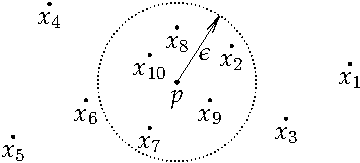
\includegraphics{figures/sequence-convergence-metric}
\caption{Sequence converging to $p$.  The first 10 points 
are shown and $M=7$ for this $\epsilon$.\label{fig:sequence-convergence-metric}}
\end{myfig}
\end{defn}

\begin{prop} \label{prop:mslimisunique}
A convergent sequence in a metric space has a unique limit.
\end{prop}

\begin{proof}
Suppose the sequence $\{ x_n \}$ has limits $x$ and $y$.
Take an arbitrary $\epsilon > 0$.
From the definition find an $n$ such that 
$d(x_n,x) < \nicefrac{\epsilon}{2}$ and
$d(x_n,y) < \nicefrac{\epsilon}{2}$.  Then
\begin{equation*}
d(y,x)
\leq
d(y,x_n) + d(x_n,x)
<
\frac{\epsilon}{2} + \frac{\epsilon}{2} = \epsilon .
\end{equation*}
So $x=y$, and the limit (if it exists) is unique.
\end{proof}

The proofs of the following propositions are left as exercises.

\begin{prop} \label{prop:msconvbound}
A convergent sequence in a metric space is bounded.
\end{prop}

\begin{prop} \label{prop:msconvifa}
A sequence $\{ x_n \}$ in a metric space $(X,d)$ converges to $p \in X$
if and only
if there exists a sequence $\{ a_n \}$ of real numbers such that
\begin{equation*}
d(x_n,p) \leq a_n \quad \text{for all } n \in \N,
\qquad \text{and} \qquad
\lim_{n\to\infty} a_n = 0.
\end{equation*}
\end{prop}

\begin{prop} \label{prop:mssubseq}
Let $\{ x_n \}$ be a sequence in a metric space $(X,d)$.
\begin{enumerate}[(i)]
\item If $\{ x_n \}$ converges to $p \in X$, then every subsequence $\{ x_{n_k} \}$
converges to $p$.
\item If for some $K \in \N$ the $K$-tail $\{ x_n \}_{n=K+1}^\infty$
converges to $p \in X$, then
 $\{ x_n \}$ converges to $p$.
\end{enumerate}
\end{prop}

\begin{exbox}
\begin{exercise}
Prove \propref{prop:msconvbound}.
\end{exercise}

\begin{exercise}
Prove \propref{prop:msconvifa}.
\end{exercise}

\begin{exercise}
Prove \propref{prop:mssubseq}.
\end{exercise}
\end{exbox}

\begin{example}
The set of continuous functions $C([a,b],\R)$, see \exampleref{example:msC01},
is a metric space.  Convergence of a sequence of functions
in this metric space is the same as uniform convergence.  See also
\sectionref{sec:puconv} in the next appendix.
\end{example}

\begin{exbox}
\begin{exercise}
\begin{exparts}
\item
Show that $d(x,y) = \min \bigl\{ 1, \sabs{x-y} \bigr\}$ defines a metric on $\R$.
\item
Show that a sequence converges in $(\R,d)$ if and only if it converges
in the standard metric.
\item
Find a bounded sequence in $(\R,d)$ that
contains no convergent subsequence.
\end{exparts}
\end{exercise}

\begin{exercise}
Suppose $\{x_n\}_{n=1}^\infty$ converges to $x$.  Suppose $f \colon \N
\to \N$ is a one-to-one function.  Show that
$\{ x_{f(n)} \}_{n=1}^\infty$ converges to $x$.
\end{exercise}

\begin{exercise}
Let $(X,d)$ be a metric space where $d$ is the discrete metric.  Suppose 
$\{ x_n \}$ is a convergent sequence in $X$.  Show that there exists
a $K \in \N$ such that for all $n \geq K$ we have $x_n = x_K$.
\end{exercise}

\begin{exercise}
A set $S \subset X$ is said to be \emph{dense} in $X$ if
$X \subset \widebar{S}$ or in other words if for every $x \in X$,
there exists a sequence $\{ x_n \}$ in $S$ that converges to $x$.  Prove
that $\R^n$ contains a countable dense subset.
\end{exercise}

\begin{exercise} \label{exercise:extendedrealsmetric}
Take $\R^* = \{ -\infty \} \cup \R \cup \{ \infty \}$ be the extended reals.
Define $d(x,y) = \babs{\frac{x}{1+\sabs{x}} - \frac{y}{1+\sabs{y}}}$
if $x, y \in \R$,
define $d(\infty,x) = \babs{1 - \frac{x}{1+\sabs{x}}}$,
$d(-\infty,x) = \babs{1 + \frac{x}{1+\sabs{x}}}$
for all $x \in \R$, and
let $d(\infty,-\infty) = 2$.
\begin{exparts}
\item
Show that $(\R^*,d)$ is a metric space.
\item
Suppose $\{ x_n \}$ is a sequence of real numbers such that
for every $M \in \R$, there exists an $N$ such that
$x_n \geq M$ for all $n \geq N$.  Show that $\lim\, x_n = \infty$ in
$(\R^*,d)$.
\item
Show that a sequence of real numbers converges to a real number
in $(\R^*,d)$ if and
only if it converges in $\R$ with the standard metric.
\end{exparts}
\end{exercise}

\begin{exercise}
Let $(X,d)$ be a metric space and $\{ x_n \}$ a sequence in $X$.
Prove that $\{ x_n \}$ converges to $p \in X$
if and only if
every subsequence of $\{ x_n \}$ has a subsequence that
converges to $p$.
\end{exercise}
\end{exbox}

\subsection{Convergence in euclidean space}

In $\R^n$, a sequence converges if and only if every
component converges:

\begin{prop} \label{prop:msconveuc}
Let $\{ x_j \}_{j=1}^\infty$ be a sequence in $\R^n$,
where $x_j = \bigl(x_{j,1},x_{j,2},\ldots,x_{j,n}\bigr) \in \R^n$.
Then $\{ x_j \}_{j=1}^\infty$ converges if and only if
$\{ x_{j,k} \}_{j=1}^\infty$ converges for every $k=1,2,\ldots,n$, in which case
\begin{equation*}
\lim_{j\to\infty}
x_j =
\Bigl(
\lim_{j\to\infty} x_{j,1},
\lim_{j\to\infty} x_{j,2},
\ldots,
\lim_{j\to\infty} x_{j,n}
\Bigr) .
\end{equation*}
\end{prop}

\begin{proof}
Suppose
the sequence
$\{ x_j \}_{j=1}^\infty$ converges to
$y = (y_1,y_2,\ldots,y_n) \in \R^n$.
Given $\epsilon > 0$, there exists an $M$, such that for all
$j \geq M$,
\begin{equation*}
d(y,x_j) < \epsilon.
\end{equation*}
Fix some $k=1,2,\ldots,n$.  For $j \geq M$,
\begin{equation*}
\bigl\lvert y_k - x_{j,k} \bigr\rvert
=
\sqrt{{\bigl(y_k - x_{j,k} \bigr)}^2}
\leq
\sqrt{\sum_{\ell=1}^n {\bigl(y_\ell-x_{j,\ell}\bigr)}^2}
= d(y,x_j) < \epsilon .
\end{equation*}
Hence the sequence $\{ x_{j,k} \}_{j=1}^\infty$ converges to $y_k$.

For the other direction, suppose 
$\{ x_{j,k} \}_{j=1}^\infty$ converges to $y_k$ for every $k=1,2,\ldots,n$.
Given $\epsilon > 0$, pick an $M$, such that if $j \geq M$, then 
$\bigl\lvert y_k-x_{j,k} \bigr\rvert < \nicefrac{\epsilon}{\sqrt{n}}$ for all
$k=1,2,\ldots,n$.  Then
\begin{equation*}
d(y,x_j)
=
\sqrt{\sum_{k=1}^n {\bigl(y_k-x_{j,k}\bigr)}^2}
<
\sqrt{\sum_{k=1}^n {\left(\frac{\epsilon}{\sqrt{n}}\right)}^2}
=
\sqrt{\sum_{k=1}^n \frac{{\epsilon^2}}{n}}
= \epsilon .
\end{equation*}
That is, the sequence $\{ x_j \}$ converges to
$y = (y_1,y_2,\ldots,y_n) \in \R^n$.
\end{proof}

\begin{example}
For $\C$, the proposition says that
$\{ z_j \}_{j=1}^\infty = \{ x_j + iy_j \}_{j=1}^\infty$ converges
to $z = x+iy$
if and only if $\{ x_j \}$ converges to $x$ and 
$\{ y_j \}$ converges to $y$.
\end{example}

\begin{exbox}
\begin{exercise}
Consider $\R^n$, and let $d$ be the standard euclidean metric.
Let $d'(x,y) = \sum_{\ell=1}^n \sabs{x_\ell-y_\ell}$
and $d''(x,y) = \max \bigl\{ \sabs{x_1-y_1},\sabs{x_2-y_2},\cdots,\sabs{x_n-y_n}
\bigr\}$.
\begin{exparts}
\item
Use \exerciseref{exercise:mscross}, to show that
$(\R^n,d')$ and
$(\R^n,d'')$ are metric spaces.
\item
Let $\{ x_j \}_{j=1}^\infty$ be a sequence in $\R^n$ and $p \in \R^n$.
Prove that the following statements are equivalent:
\begin{exnumparts}
\item
$\{ x_j \}$ converges to $p$ in $(\R^n,d)$.
\item
$\{ x_j \}$ converges to $p$ in $(\R^n,d')$.
\item
$\{ x_j \}$ converges to $p$ in $(\R^n,d'')$.
\end{exnumparts}
\end{exparts}
\end{exercise}
\end{exbox}

\subsection{Convergence and topology}

The topology---the set of open sets of a space---encodes which
sequences converge.

\begin{prop} \label{prop:msconvtopo}
Let $(X,d)$ be a metric space and $\{x_n\}$ a sequence in $X$.  Then
$\{ x_n \}$ converges to $x \in X$ if and only if for every open neighborhood
$U$ of $x$, there exists an $M \in \N$ such that for all $n \geq M$
we have $x_n \in U$.
\end{prop}

\begin{proof}
Suppose $\{ x_n \}$ converges to $x$.  Let $U$ be an open neighborhood
of $x$, then there exists an $\epsilon > 0$ such that $B(x,\epsilon) \subset
U$.  As the sequence converges, find an $M \in \N$ such that for all $n \geq
M$ we have $d(x,x_n) < \epsilon$, or in other words $x_n \in B(x,\epsilon)
\subset U$.

Let us prove the other direction.  Given $\epsilon > 0$, let $U =
B(x,\epsilon)$ be the neighborhood of $x$.  Then there is an $M \in \N$
such that for $n \geq M$ we have $x_n \in U = B(x,\epsilon)$ or in other
words, $d(x,x_n) < \epsilon$.
\end{proof}

A closed set contains the limits of its convergent sequences.

\begin{prop} \label{prop:msclosedlim}
Let $(X,d)$ be a metric space, $E \subset X$ a closed set,
and $\{ x_n \}$ a sequence in $E$ that converges to some $x \in X$.
Then $x \in E$.
\end{prop}

\begin{proof}
Let us prove the contrapositive.
Suppose $\{ x_n \}$ is a sequence in $X$ that converges to $x \in E^c$.
As $E^c$ is open, \propref{prop:msconvtopo} says that there is
an $M$ such that for all $n \geq M$,
$x_n \in E^c$.  So $\{ x_n \}$  is not a sequence in $E$.
\end{proof}

To take a closure of a set $A$, we take $A$, and we throw in 
points that are limits of sequences in $A$.

\begin{prop} \label{prop:msclosureapprseq}
Let $(X,d)$ be a metric space and $A \subset X$.
Then $x \in \widebar{A}$ if and only if there exists a sequence $\{ x_n \}$ of
elements in $A$ such that $\lim\, x_n = x$.
\end{prop}

\begin{proof}
Let $x \in \widebar{A}$.  For every $n \in \N$,
by
\propref{prop:msclosureappr} there
exists a point $x_n \in B(x,\nicefrac{1}{n}) \cap A$.
As $d(x,x_n) < \nicefrac{1}{n}$, we have $\lim\, x_n = x$.

For the other direction, see \exerciseref{exercise:reverseclosedseq}.
\end{proof}

\begin{exbox}
\begin{exercise}%[\neededexmark]
\label{exercise:reverseclosedseq}
Finish the proof of 
\propref{prop:msclosureapprseq}.
Let $(X,d)$ be a metric space and
let $A \subset X$.  Let $E$ be the set of all $x \in X$ such that there
exists a sequence $\{ x_n \}$ in $A$ that converges to $x$.  Show 
$E = \widebar{A}$.
\end{exercise}

\begin{exercise}
Suppose $\{ U_n \}_{n=1}^\infty$ is a decreasing ($U_{n+1} \subset U_n$ for
all $n$) sequence of open sets in a metric space $(X,d)$ such that
$\bigcap_{n=1}^\infty U_n = \{ p \}$ for some $p \in X$.  Suppose 
$\{ x_n \}$ is a sequence of points in $X$ such that $x_n \in U_n$.  Does
$\{ x_n \}$ necessarily converge to $p$?  Prove or construct a counterexample.
\end{exercise}

\begin{exercise}
Let $E \subset X$ be closed and
let $\{ x_n \}$ be a sequence in $X$ converging to $p \in X$.  Suppose
$x_n \in E$ for infinitely many $n \in \N$.  Show $p \in E$.
\end{exercise}

\begin{exercise}
Suppose $\{ V_n \}_{n=1}^\infty$ is a sequence of open sets
in $(X,d)$
such that $V_{n+1} \supset V_n$ for all $n$.  Let $\{ x_n \}$ be a sequence
such that $x_n \in V_{n+1} \setminus V_n$ and suppose 
$\{ x_n \}$ converges to $p \in X$.  Show that $p \in \partial V$
where $V = \bigcup_{n=1}^\infty V_n$.
\end{exercise}
\end{exbox}

%%%%%%%%%%%%%%%%%%%%%%%%%%%%%%%%%%%%%%%%%%%%%%%%%%%%%%%%%%%%%%%%%%%%%%%%%%%%%%

\section{Completeness and compactness}
\label{sec:metcompact}

\subsection{Cauchy sequences and completeness}

\begin{defn}
Let $(X,d)$ be a metric space.
A sequence $\{ x_n \}$ in $X$ is a \emph{\myindex{Cauchy sequence}} if
for every $\epsilon > 0$ there exists an $M \in \N$ such that
for all $n \geq M$ and all $k \geq M$ we have
\begin{equation*}
d(x_n, x_k) < \epsilon .
\end{equation*}
\end{defn}

\begin{prop}
A convergent sequence in a metric space is Cauchy.
\end{prop}

\begin{proof}
Suppose $\{ x_n \}$ converges to $x$.
Given $\epsilon > 0$, there is an $M$ such that
$d(x,x_n) < \nicefrac{\epsilon}{2}$ for all $n \geq M$.
Hence,
$d(x_n,x_k) \leq d(x_n,x) + d(x,x_k) < \nicefrac{\epsilon}{2} +
\nicefrac{\epsilon}{2} = \epsilon$
for all $n,k \geq M$.
\end{proof}

\begin{defn}
Let $(X,d)$ be a metric space.  We say $X$ is
\emph{\myindex{complete}} or \emph{\myindex{Cauchy-complete}}
if every Cauchy sequence $\{ x_n \}$ in $X$
converges to an $x \in X$.
\end{defn}

\begin{prop}
The space $\R^n$ with the standard metric is a complete metric space.
\end{prop}

We assume the reader has seen the proof of completeness in $\R = \R^1$,
and we reduce the completeness in $\R^n$ to the one dimensional case.

\begin{proof}
Let $\{ x_j \}_{j=1}^\infty$ be a Cauchy sequence
in $\R^n$, where $x_j = \bigl(x_{j,1},x_{j,2},\ldots,x_{j,n}\bigr) \in \R^n$.
Given $\epsilon > 0$, there exists an $M$ such that
$d(x_i,x_j) < \epsilon$
for all
$i,j \geq M$.

Fix some $k=1,2,\ldots,n$.  For $i,j \geq M$,
\begin{equation*}
\bigl\lvert x_{i,k} - x_{j,k} \bigr\rvert
=
\sqrt{{\bigl(x_{i,k} - x_{j,k}\bigr)}^2}
\leq
\sqrt{\sum_{\ell=1}^n {\bigl(x_{i,\ell}-x_{j,\ell}\bigr)}^2}
= d(x_i,x_j) < \epsilon .
\end{equation*}
Hence the sequence $\{ x_{j,k} \}_{j=1}^\infty$ is Cauchy.  As $\R$ is
complete the sequence converges; there exists a $y_k \in \R$ such that
$y_k = \lim_{j\to\infty} x_{j,k}$.
Write $y = (y_1,y_2,\ldots,y_n) \in \R^n$.
By \propref{prop:msconveuc}, $\{ x_j \}$ converges
to $y \in \R^n$, and hence $\R^n$ is complete.
\end{proof}

A subset of $\R^n$ with the subspace metric need not be
complete.  For example, $(0,1]$ with the subspace metric is not
complete as $\{ \nicefrac{1}{n} \}$ is a Cauchy sequence in $(0,1]$
with no limit in $(0,1]$.
However,
once we have one complete metric space, any closed subspace is
also a complete metric space.  After all, one way
to think of a closed set is that it contains all points
that can be reached from the set via a sequence.
The proof is again an exercise.

\begin{prop} \label{prop:closedcomplete}
Suppose $(X,d)$ is a complete metric space and $E \subset X$
is closed, then $E$ is a complete metric space with the subspace topology.
\end{prop}

\begin{exbox}
\begin{exercise}%[\neededexmark]
Prove \propref{prop:closedcomplete}.
\end{exercise}
\end{exbox}

\begin{example}
Another very useful example of a complete metric space is the space of
continuous functions on a closed interval with the uniform norm, $C([a,b],\R)$.
See \corref{cor:CSRcomplete} in the next appendix.
\end{example}

\subsection{Compactness}

\begin{defn}
Let $(X,d)$ be a metric space and $K \subset X$. 
The set $K$ is said to be \emph{\myindex{compact}}
if for any collection
of open sets $\{ U_{\lambda} \}_{\lambda \in I}$ such that
\begin{equation*}
K \subset \bigcup_{\lambda \in I} U_\lambda ,
\end{equation*}
there exists a finite subset
$\{ \lambda_1, \lambda_2,\ldots,\lambda_k \} \subset I$
such that
\begin{equation*}
K \subset U_{\lambda_1} \cup U_{\lambda_2} \cup \cdots \cup U_{\lambda_k} .
\end{equation*}
\end{defn}

A collection of open sets $\{ U_{\lambda} \}_{\lambda \in I}$ as above is
said to be an \emph{\myindex{open cover}} of $K$.  A way to say that
$K$ is compact is to say that \emph{every open cover of $K$ has a finite
\myindex{subcover}}.

\begin{example}
Let $\R$ be the metric space with the standard metric.

The set $\R$ is not compact.  Proof: Take the sets $U_n = (-n,n)$.
It is an open cover, but the union of a finite subset of these sets
is just $(-n,n)$ for some $n$.

The set $(0,1) \subset \R$ is also not compact.  Proof:  Take the 
sets $U_{n} = (\nicefrac{1}{n},1-\nicefrac{1}{n})$ for $n=3,4,5,\ldots$.
As above $(0,1) = \bigcup_{n=3}^\infty U_n$, but the union of finitely many
is just $U_n$ again and not all of $(0,1)$.

The set $\{ 0 \} \subset \R$ is compact.  Proof: Given any open cover $\{
U_{\lambda} \}_{\lambda \in I}$, there must exist a $\lambda_0$ such that $0
\in U_{\lambda_0}$ as it is a cover, so $U_{\lambda_0}$ gives a
finite subcover.

We will prove below that $[0,1]$, and in fact any closed and bounded
interval $[a,b]$ is compact.
\end{example}

\begin{exbox}
\begin{exercise}
Let $(X,d)$ be a metric space and $A$ a finite subset of $X$.
Show that $A$ is compact.
\end{exercise}

\begin{exercise}
Let $A = \{ \nicefrac{1}{n} : n \in \N \} \subset \R$.
\begin{exparts}
\item
Show that $A$ is
not compact directly using the definition.
\item
Show that $A \cup \{ 0 \}$ is
compact directly using the definition.
\end{exparts}
\end{exercise}

\begin{exercise}
\begin{exparts}
\item
Show that the union of finitely many compact sets is a compact set.
\item
Find an example where the union of infinitely many compact sets is not
compact.
\end{exparts}
\end{exercise}
\end{exbox}

\begin{prop}
Let $(X,d)$ be a metric space.  A compact set $K \subset X$ is closed and
bounded.
\end{prop}

\begin{proof}
Let $K$ be a compact set.
Fix $p \in X$.  We have the open cover
\begin{equation*}
K \subset \bigcup_{n=1}^\infty B(p,n) = X .
\end{equation*}
If $K$ is compact, then there exists some set of indices
$n_1 < n_2 < \ldots < n_k$ such that
\begin{equation*}
K \subset
B(p,n_1)
\cup
B(p,n_2)
\cup \cdots \cup
B(p,n_k)
= B(p,n_k) .
\end{equation*}
So $K$ is bounded.
See left-hand side of \figureref{fig:compactbndclosed}.

Next, we show a set that is not closed is not compact.  Suppose 
$\widebar{K} \not= K$, that is, there is a point $x \in \widebar{K}
\setminus K$.
We have the open cover
\begin{equation*}
K \subset \bigcup_{n=1}^\infty {C(x,\nicefrac{1}{n})}^c .
\end{equation*}
If we take any
finite collection of indices $n_1 < n_2 < \ldots < n_k$, then 
\begin{equation*}
{C(x,\nicefrac{1}{n_1})}^c 
\cup
{C(x,\nicefrac{1}{n_2})}^c 
\cup \cdots \cup
{C(x,\nicefrac{1}{n_k})}^c 
=
{C(x,\nicefrac{1}{n_k})}^c 
\end{equation*}
As $x$ is in the closure of $K$,
then
$C(x,\nicefrac{1}{n_k}) \cap K \not= \emptyset$.  So there is no
finite subcover and $K$ is not compact.
See right-hand side of \figureref{fig:compactbndclosed}.
\end{proof}

\begin{myfig}
\subimport*{figures/}{compactbnd.pdf_t}
\qquad \qquad
\subimport*{figures/}{compactclosed.pdf_t}
\caption{Proving compact set is bounded (left) and closed (right).\label{fig:compactbndclosed}}
\end{myfig}

We prove below that 
in a finite dimensional euclidean space
every closed bounded set is compact.
So closed bounded sets
of $\R^n$ are examples of compact sets.
It is not true that in every metric space, closed and bounded is equivalent
to compact.  A simple example is an incomplete metric space such as
$(0,1)$ with the subspace metric from $\R$.
There are many complete and very useful metric spaces
where closed and bounded is not
enough to give compactness: $C([a,b],\R)$ is a complete metric
space, but the closed unit ball $C(0,1)$ is not compact, see
\exerciseref{exercise:msclbounnotcompt}.  However, see also
\exerciseref{exercise:mstotbound}.  As this issue is such a common mistake, let me
repeat it in italic: \emph{Closed and bounded is not the same as compact.}

A useful property of compact sets in a metric space is that every
sequence in the set has a convergent subsequence converging
to a point in the set.
Such sets are called
\emph{\myindex{sequentially compact}}.
Let us prove that in the
context of metric spaces, a set is compact if and only if it is sequentially
compact.
First we prove a lemma.

\begin{lemma}[Lebesgue covering lemma%
\footnote{The number $\delta$ is sometimes called the
\myindex{Lebesgue number} of the cover.}]\label{ms:lebesgue}
\index{Lebesgue covering lemma}
Let $(X,d)$ be a metric space and $K \subset X$.  Suppose 
every sequence in $K$ has a subsequence convergent in $K$.  Given
an open cover $\{ U_\lambda \}_{\lambda \in I}$ of $K$, there exists a
$\delta > 0$ such that for every $x \in K$, there exists a $\lambda \in I$
with $B(x,\delta) \subset U_\lambda$.
\end{lemma}

\begin{proof}
We prove the lemma by contrapositive.
If the conclusion is not true, then
there is
an open cover $\{ U_\lambda \}_{\lambda \in I}$ of $K$ with
the following property.
For every $n \in \N$ there exists an $x_n \in K$ such that
$B(x_n,\nicefrac{1}{n})$ is not a subset of any $U_\lambda$.
Take any $x \in K$.  There is
a $\lambda \in I$ such that $x \in U_\lambda$.  As $U_\lambda$ is open,
there is an $\epsilon > 0$ 
such that $B(x,\epsilon) \subset U_\lambda$.  Take $M$ such that
$\nicefrac{1}{M} < \nicefrac{\epsilon}{2}$.  If $y \in 
B(x,\nicefrac{\epsilon}{2})$ and $n \geq M$, then 
\begin{equation*}
B(y,\nicefrac{1}{n}) \subset
B(y,\nicefrac{1}{M}) \subset
B(y,\nicefrac{\epsilon}{2}) \subset B(x,\epsilon)
\subset U_\lambda ,
\end{equation*}
where 
$B(y,\nicefrac{\epsilon}{2}) \subset B(x,\epsilon)$
follows by triangle inequality.
See \figureref{fig:lebesguedelta}.
In other words, for all $n \geq M$, $x_n \notin B(x,\nicefrac{\epsilon}{2})$. 
The sequence cannot have a subsequence converging to $x$.  As $x \in K$ was
arbitrary we are done.
\end{proof}

\begin{myfig}
\subimport*{figures/}{lebesguedelta.pdf_t}
\caption{Proof of Lebesgue covering lemma.
Note that $B(y,\nicefrac{\epsilon}{2}) \subset
B(x,\epsilon)$ by triangle inequality.\label{fig:lebesguedelta}}
\end{myfig}

It is important to recognize what the lemma says.  It says that
if $K$ is sequentially compact, then given any
cover there is a single $\delta > 0$.  The $\delta$ depends on the cover,
but of course it does not depend on $x$.

For example, let $K = [-10,10]$ and for $n \in \Z$ let $U_n =
(n,n+2)$ define an open cover.
Take $x \in K$. There is an $n \in \Z$, 
such that $n \leq x < n+1$.
If $n \leq x < n+\nicefrac{1}{2}$, then
$B\bigl(x,\nicefrac{1}{2}\bigr) \subset U_{n-1}$.
If $n+ \nicefrac{1}{2} \leq x < n+1$, then
$B\bigl(x,\nicefrac{1}{2}\bigr) \subset U_{n}$.  So $\delta =
\nicefrac{1}{2}$.  If instead we take the open cover by $U'_n =
\bigl(\frac{n}{2},\frac{n+2}{2} \bigr)$, the best $\delta$ is $\nicefrac{1}{4}$.

\begin{thm} \label{thm:mscompactisseqcpt}
Let $(X,d)$ be a metric space.  Then $K \subset X$ is compact if
and only if every sequence in $K$ has a subsequence converging to
a point in $K$.
\end{thm}

\begin{proof}
Claim: \emph{Let $K \subset X$ be a subset of $X$ and
$\{ x_n \}$ a sequence in $K$.  Suppose that for each $x \in K$,
there is a ball $B(x,\alpha_x)$ for some $\alpha_x > 0$ such that
$x_n \in B(x,\alpha_x)$ for only finitely many $n \in \N$.
Then $K$ is not compact.}

Proof of the claim:
Notice
\begin{equation*}
K \subset \bigcup_{x \in K} B(x,\alpha_x) .
\end{equation*}
Any finite collection of these balls is going to contain only finitely many
$x_n$.  Thus for any finite collection of such balls there is an $x_n \in K$
that is not in the union.  Therefore, $K$ is not compact and the claim is
proved.

Suppose $K$ is compact and $\{ x_n \}$ is a sequence in $K$.
Then there exists an $x \in K$ such that
for any $\delta > 0$,
$B(x,\delta)$ contains $x_k$ for infinitely many $k \in \N$.
%We define the subsequence inductively.
The ball $B(x,1)$ contains some $x_k$ so let $n_1 = k$.
Suppose $n_{j-1}$ is defined.
There must exist an $\ell > n_{j-1}$
such that $x_\ell \in B(x,\nicefrac{1}{j})$.  So define
$n_j = \ell$.
We now posses a subsequence $\{ x_{n_j} \}_{j=1}^\infty$.
Since
$d(x,x_{n_j}) < \nicefrac{1}{j}$,  \propref{prop:msconvifa} says
$\lim\, x_{n_j} = x$.

For the other direction, suppose every sequence in $K$
has a 
subsequence converging in $K$.
Take
an open cover $\{ U_\lambda \}_{\lambda \in I}$ of $K$.
Using the Lebesgue covering lemma above, find a $\delta > 0$
such that for every $x \in K$, there is a $\lambda \in I$ with
$B(x,\delta) \subset U_\lambda$.

Pick $x_1 \in K$ and find $\lambda_1 \in I$ such that $B(x_1,\delta) \subset
U_{\lambda_1}$.
If $K \subset U_{\lambda_1}$, we stop as we have found a
finite subcover.
Otherwise, there must be
a point $x_2 \in K \setminus U_{\lambda_1}$.
Note that $d(x_2,x_1) \geq \delta$.
There must exist some $\lambda_2 \in I$ such that
$B(x_2,\delta) \subset U_{\lambda_2}$.
We work inductively.  Suppose $\lambda_{n-1}$ is defined.
Either
$U_{\lambda_1} \cup
U_{\lambda_2} \cup \cdots \cup
U_{\lambda_{n-1}}$ is a finite cover of $K$, in which case we
stop, or
there must be 
a point $x_n \in K \setminus \bigl( U_{\lambda_1} \cup
U_{\lambda_2} \cup \cdots \cup
U_{\lambda_{n-1}}\bigr)$.
Note that $d(x_n,x_j) \geq \delta$ for all $j = 1,2,\ldots,n-1$.
Next, there must be some $\lambda_n \in I$
such that $B(x_n,\delta) \subset U_{\lambda_n}$.
See \figureref{fig:seqcompactiscompact}.

\begin{myfig}
\subimport*{figures/}{seqcompactiscompact.pdf_t}
\caption{Covering $K$ by $U_{\lambda}$.  The points
$x_1,x_2,x_3,x_4$, 
the three sets 
$U_{\lambda_1}$,
$U_{\lambda_2}$,
$U_{\lambda_2}$,
and 
the first three balls
of radius $\delta$ are drawn.\label{fig:seqcompactiscompact}}
\end{myfig}

Either at some point we obtain a finite subcover of $K$,
or we obtain an
infinite
sequence $\{ x_n \}$ as above.
For contradiction, suppose that
there is no finite subcover and we have the sequence $\{ x_n \}$.
For all $n$ and $k$, $n \not= k$, 
we have $d(x_n,x_k) \geq \delta$,
so no subsequence of $\{ x_n \}$ can be
Cauchy.  Hence no subsequence of $\{ x_n \}$ can be convergent,
which is a contradiction.
\end{proof}

\begin{example}
The Bolzano--Weierstrass theorem for sequences of real numbers
says that a bounded sequence in $\R$ has a convergent
subsequence.  Therefore, any sequence in a closed interval $[a,b] \subset \R$ has 
a convergent subsequence.  The limit must also be in $[a,b]$ as limits
preserve non-strict inequalities.  Hence a closed bounded interval $[a,b]
\subset \R$ is compact.
\end{example}

\begin{prop}
Let $(X,d)$ be a metric space and let $K \subset X$ be compact.  If
$E \subset K$ is a closed set, then $E$ is compact.
\end{prop}

\begin{proof}
Because $K$ is closed then $E$ is closed in $K$ if
and only if it is closed in $X$,
see \propref{prop:topology:subspacesame}.
Let $\{ x_n \}$ be a sequence in $E$.  It is also a sequence in $K$.
Therefore, it has a convergent subsequence $\{ x_{n_j} \}$ that converges to
some $x \in K$.  As $E$ is closed the limit of a sequence in $E$ is also in $E$
and so $x \in E$.  Thus $E$ must be compact.
\end{proof}

\begin{thm}[Heine--Borel] \index{Heine--Borel theorem}
\label{thm:msbw}
A closed bounded subset $K \subset \R^n$ is compact.
\end{thm}

So subsets of $\R^n$ are compact if and only if they are closed and bounded,
a condition that is much easier to check.
Let us reiterate that the Heine--Borel theorem only holds for $\R^n$ and not
for metric spaces in general.  In general, compact implies closed and
bounded, but not vice versa.

\begin{proof}
For $\R = \R^1$ if $K \subset \R$ is closed and bounded, then
any sequence $\{ x_k \}$ in $K$ is bounded, so it has a convergent
subsequence by
the Bolzano--Weierstrass theorem.
As $K$ is closed, the limit of the subsequence must be an element of
$K$.  So $K$ is compact.

Let us carry out the proof for $n=2$ and leave arbitrary $n$ as an exercise.
As $K \subset \R^2$ is bounded, there exists a set
$B=[a,b]\times[c,d] \subset \R^2$ such that $K \subset B$.  We will show
that $B$ is compact.  Then $K$, being a closed subset of a compact $B$, is
also compact.  

Let $\bigl\{ (x_k,y_k) \bigr\}_{k=1}^\infty$ be a sequence in $B$.  That is,
$a \leq x_k \leq b$ and
$c \leq y_k \leq d$ for all $k$.  A bounded sequence of real numbers
has a convergent
subsequence so there is a subsequence $\{ x_{k_j} \}_{j=1}^\infty$
that is convergent.  The subsequence 
$\{ y_{k_j} \}_{j=1}^\infty$ is also a bounded sequence so there exists
a subsequence
$\{ y_{k_{j_\ell}} \}_{\ell=1}^\infty$ that is convergent.  A subsequence of a
convergent sequence is still convergent, so 
$\{ x_{k_{j_\ell}} \}_{\ell=1}^\infty$ is convergent.
Let
\begin{equation*}
x = \lim_{\ell\to\infty} x_{k_{j_\ell}}
\qquad \text{and} \qquad
y = \lim_{\ell\to\infty} y_{k_{j_\ell}} .
\end{equation*}
By \propref{prop:msconveuc},
$\bigl\{ (x_{k_{j_\ell}},y_{k_{j_\ell}}) \bigr\}_{\ell=1}^\infty$ converges to $(x,y)$.
As $a \leq x_k \leq b$ and
$c \leq y_k \leq d$ for all $k$, we know that $(x,y) \in B$.
\end{proof}

\begin{exbox}
\begin{exercise}
Prove \thmref{thm:msbw} for arbitrary dimension.
Hint: The trick is to use the correct notation.
\end{exercise}
\end{exbox}

\begin{prop}
Suppose $(X,d)$ is a metric space
and $E_1$, $E_2$, \ldots, are
nonempty compact subsets of $X$ such that
$E_1 \supset E_2 \supset E_3 \supset \cdots$.  Then
\begin{equation*}
\bigcap_{k=1}^\infty E_k \not= \emptyset .
\end{equation*}
\end{prop}

\begin{proof}
Suppose $E_1,E_2,\ldots$ are as in the statement except we do not
assume they are nonempty.
Compact sets are closed so their complement is open.  Consider
$U_k = X \setminus E_k$.  Suppose that the intersection is empty.
Then $\{ U_k \}$ is an open cover of $E_1$, which is compact,
and hence there is a finite subcover.
As the sets are nested,
$U_\ell \subset U_{\ell+1}$ for all $\ell$,
we have $E_1 \subset U_k$ for some $k$.   Thus $E_k$ is empty.
\end{proof}

\begin{example}
Let $(X,d)$ be a metric space with the discrete metric, that is, $d(x,y) = 1$
if $x \not= y$.  Suppose
$X$ is an infinite set.  Then:
\begin{enumerate}[(i)]
\item $(X,d)$ is a complete metric space.
\item Any subset $K \subset X$ is closed and bounded.
\item A subset $K \subset X$ is compact if and only if it is a finite set.
\item The conclusion of the Lebesgue covering lemma is always satisfied
with any $\delta \in (0,1)$, even for noncompact $K \subset X$.
\end{enumerate}
The proofs
of the statements are either trivial or are relegated to the exercises
below.
\end{example}

\begin{remark}
A subtle point about Cauchy sequences, completeness, compactness,
and convergence is that compactness and convergence only depend on the
topology, that is, on which sets are the open sets.  On the other hand,
Cauchy sequences and completeness depend on the actual metric.
\end{remark}

\begin{exbox}
\begin{exercise}
Let $(X,d)$ be a metric space with the discrete metric.
\begin{exparts}
\item
Prove that $X$ is complete.
\item
Prove that $X$ is compact if and only if $X$ is a finite set.
\end{exparts}
\end{exercise}

\begin{exercise}
Show that a compact set $K$ is a complete metric space (using the subspace
metric).
\end{exercise}

\begin{exercise}
Show that there exists a metric on $\R$ that makes $\R$ into a compact set.
\end{exercise}

\begin{exercise} \label{exercise:msclbounnotcompt}
Let $C([0,1],\R)$ be the metric space of \exampleref{example:msC01}.  Let $0$
denote the zero function.  Show that the closed ball
$C(0,1)$ is not compact (even though it is closed and bounded).
Hint: Construct continuous functions $f_n \colon [0,1] \to \R$ such that
$d(f_n,0) = 1$ and $d(f_n,f_k) = 1$ for all $n \not= k$.
\end{exercise}

\begin{exercise}
Let $C([0,1],\R)$ be the metric space of \exampleref{example:msC01}.
Let $K$ be the set of $f \in C([0,1],\R)$ such that
$f$ is equal to a quadratic polynomial, i.e., $f(x) = a+bx+cx^2$, and such that
$\abs{f(x)} \leq 1$ for all $x \in [0,1]$,
that is $f \in C(0,1)$.  Show that $K$ is compact.
\end{exercise}

\begin{exercise} \label{exercise:mstotbound}
Let $(X,d)$ be a complete metric space.
Show that $K \subset X$ is compact if and only if $K$ is closed
and such that for every $\epsilon > 0$
there exists a finite set of points $x_1,x_2,\ldots,x_n$ with
$K \subset \bigcup_{j=1}^n B(x_j,\epsilon)$.
Note: Such a set $K$ is said to be \emph{\myindex{totally bounded}},
so in a complete metric space a set is compact if and only
if it is closed and totally bounded.
\end{exercise}

\begin{exercise}
Take $\N \subset \R$ using the standard metric.  Find an open cover of $\N$
such that the conclusion of the Lebesgue covering lemma does not hold.
\end{exercise}

\begin{exercise}
Prove the general \myindex{Bolzano--Weierstrass theorem}:
Any bounded sequence $\{ x_k
\}$ in $\R^n$ has a convergent subsequence.
\end{exercise}

\begin{exercise}
Let $X$ be a metric space and
$C$ the set of nonempty compact subsets of $X$.
Using the Hausdorff metric from \exerciseref{exercise:mshausdorffpseudo},
show that $(C,d_H)$ is a metric space.  That is, show that
if $L$ and $K$ are nonempty compact subsets, then $d_H(L,K) = 0$
if and only if $L=K$.
\end{exercise}

\begin{exercise}
Let $(X,d)$ be an incomplete metric space.  Show that there exists a
closed and bounded set $E \subset X$ that is not compact.
\end{exercise}

\begin{exercise}
Let $(X,d)$ be a metric space and $K \subset X$.
Prove that $K$ is compact as a subset of $(X,d)$ if and only if $K$ is
compact as a subset of itself with the subspace metric.
\end{exercise}

\begin{exercise}
Let $(X,d)$ be a complete metric space.
We say a set $S \subset X$ is \emph{\myindex{relatively compact}}
if the closure $\widebar{S}$ is compact.
Prove that $S \subset X$ is relatively compact if and only if
given any sequence $\{ x_n \}$ in $S$, there exists a subsequence
$\{ x_{n_k} \}$ that converges (in $X$).
\end{exercise}
\end{exbox}

%%%%%%%%%%%%%%%%%%%%%%%%%%%%%%%%%%%%%%%%%%%%%%%%%%%%%%%%%%%%%%%%%%%%%%%%%%%%%%

\section{Continuous functions}
\label{sec:metcont}

\subsection{Continuity}

\begin{defn}
Let $(X,d_X)$ and $(Y,d_Y)$ be metric spaces and $c \in X$.
Then $f \colon X \to Y$ is
\emph{continuous at $c$}\index{continuous at $c$}
if for every $\epsilon > 0$
there is a $\delta > 0$ such that whenever $x \in X$ and $d_X(x,c) <
\delta$, then
$d_Y\bigl(f(x),f(c)\bigr) < \epsilon$.

If $f \colon X \to Y$ is continuous at all $c \in X$, then we say
that $f$ is a \emph{continuous function}\index{continuous function!in a
metric space}\index{function!continuous}.
\end{defn}

\begin{prop} \label{prop:contiscont}
Let $(X,d_X)$ and $(Y,d_Y)$ be metric spaces.
Then $f \colon X \to Y$ is
continuous at $c \in X$
if and only if for every sequence $\{ x_n \}$ in $X$
converging to $c$, the sequence $\{ f(x_n) \}$ converges
to $f(c)$.
\end{prop}

\begin{proof}
Suppose $f$ is continuous at $c$.  Let $\{ x_n \}$ be a
sequence in $X$ converging to $c$.  Given $\epsilon > 0$,
there is a $\delta > 0$ such that $d_X(x,c) < \delta$ implies
$d_Y\bigl(f(x),f(c)\bigr) < \epsilon$.  So take $M$ such that
for all $n \geq M$, we have $d_X(x_n,c) < \delta$, then
$d_Y\bigl(f(x_n),f(c)\bigr) < \epsilon$.  Hence $\{ f(x_n) \}$
converges to $f(c)$.

Now suppose $f$ is not continuous at $c$.
Then there exists an $\epsilon > 0$,
such that for every $n \in \N$ there is an $x_n \in X$,
with
$d_X(x_n,c) < \nicefrac{1}{n}$ such that $d_Y\bigl(f(x_n),f(c)\bigr) \geq
\epsilon$.  So $\{ x_n \}$ converges to $c$, but $\{ f(x_n) \}$
does not converge to $f(c)$.
\end{proof}

\begin{example}
Suppose $f \colon \R^2 \to \R$ is a polynomial.  That is,
\begin{equation*}
\begin{split}
f(x,y) & =
\sum_{k=0}^d
\sum_{\ell=0}^{d-k}
a_{k\ell}\,x^ky^\ell \\
& =
a_{0\,0} + a_{1\,0} \, x +
a_{0\,1} \, y+  
a_{2\,0} \, x^2+  
a_{1\,1} \, xy+  
a_{0\,2} \, y^2+ \cdots +
a_{0\,d} \, y^d ,
\end{split}
\end{equation*}
for some $d \in \N$ (the degree) and $a_{k\ell} \in \R$.  Then we claim 
$f$ is continuous.  Let $\{ (x_n,y_n) \}_{n=1}^\infty$ be a sequence
in $\R^2$ that converges to $(x,y) \in \R^2$.  We proved that this
means $\lim\, x_n = x$ and $\lim\, y_n = y$.  Then
\begin{equation*}
\lim_{n\to\infty}
f(x_n,y_n) =
\lim_{n\to\infty}
\sum_{k=0}^d
\sum_{\ell=0}^{d-k}
a_{k\ell} \, x_n^ky_n^\ell 
=
\sum_{k=0}^d
\sum_{\ell=0}^{d-k}
a_{k\ell} \, x^ky^\ell
=
f(x,y) .
\end{equation*}
So $f$ is continuous at $(x,y)$, and as $(x,y)$ was arbitrary $f$ is
continuous everywhere.  Similarly, a
polynomial in $n$ variables is continuous.
\end{example}

Be careful about taking limits separately.  It is not enough that
for every $y$, the function $g(x) = f(x,y)$ is
continuous, and for every $x$, the function $h(y) = f(x,y)$
is continuous.  The function $f(x,y)$ could still be discontinuous.

\begin{exbox}
\begin{exercise}
Let $f \colon \R^2 \to \R$ be defined by $f(0,0) = 0$, and
$f(x,y) = \frac{xy}{x^2+y^2}$ if $(x,y) \not= (0,0)$.
See \figureref{fig:xyxsqysq}.
\begin{exparts}
\item
Show that for each fixed $x$,
the function that takes $y$ to $f(x,y)$ is continuous.  Similarly
for each fixed $y$, the function that takes $x$ to $f(x,y)$ is continuous.
\item
Show that $f$ is not continuous.
\end{exparts}
\end{exercise}
\end{exbox}

\begin{myfig}
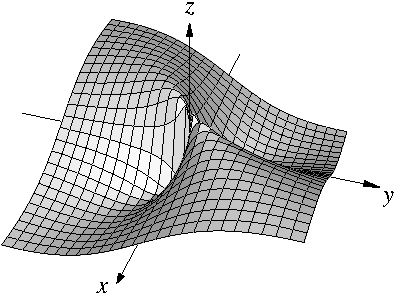
\includegraphics{figures/xyxsqysq}
\caption{Graph of $\frac{xy}{x^2+y^2}$.\label{fig:xyxsqysq}}
\end{myfig}

\begin{example}
Consider
$f \colon X \to \C$ 
on a metric space $X$.
Write $f(p) = u(p) + i v(p)$, where $u \colon X \to \R$
and $v \colon X \to \R$ are the real and imaginary parts.
Then $f$ is continuous at $c \in X$ if and only if its real
and imaginary parts are continuous at $c$.  
This fact follows because $\bigl\{ f(p_n) = u(p_n) + i v(p_n) \bigr\}_{n=1}^\infty$
converges to $f(p) = u(p) + i v(p)$ if and only if
$\bigl\{ u(p_n) \bigl\}$ converges to $u(p)$ and
$\bigl\{ v(p_n) \bigl\}$ converges to $v(p)$.
\end{example}

\begin{prop}\label{prop:distcont}
Let $(X,d)$ be a metric space.
\begin{enumerate}[(i)]
\item\label{prop:distcont:i}
If $p \in X$,
then $f \colon X \to \R$ defined
by $f(x) = d(x,p)$ is continuous.
\item\label{prop:distcont:ii}
Given a nonempty set $S \subset X$, the function
\begin{equation*}
f(x) = \inf_{p \in S} d(x,p)
\end{equation*}
is continuous.
\end{enumerate}
\end{prop}

\begin{proof}
The reverse triangle inequality
$\sabs{f(x)-f(y)} = \sabs{d(x,p)-d(y,p)} \leq d(x,y)$
gives part \ref{prop:distcont:i}.

For \ref{prop:distcont:ii}, $S$ being nonempty implies that $f$ is
real-valued.  For any $\epsilon > 0$, there exists a $q$ such that
$\inf_{p \in S} d(y,p) \geq d(y,q) + \epsilon$.  Suppose that $f(x) > f(y)$.
Then again the reverse triangle inequality gives
\begin{equation*}
f(x)-f(y) =
\inf_{p \in S} d(x,p)
-
\inf_{p \in S} d(y,p)
\leq
\inf_{p \in S} d(x,p) - d(y,q) + \epsilon 
\leq d(x,y) + \epsilon.
\avoidbreak
\end{equation*}
Since it holds for every $\epsilon$, $f$ is continuous.
\end{proof}

\begin{exbox}
\begin{exercise} \label{exercise:continuousintoperator}
Take the metric space of continuous functions $C([0,1],\R)$.  Let
$k \colon [0,1] \times [0,1] \to \R$ be a continuous function.
Given $f \in C([0,1],\R)$ define
\begin{equation*}
\varphi_f(x) = \int_0^1 k(x,y) f(y)  \, dy .
\end{equation*}
\begin{exparts}
\item
Show that $T(f) = \varphi_f$ defines a function $T \colon C([0,1],\R) \to
C([0,1],\R)$.
\item
Show that $T$ is continuous.
\end{exparts}
\end{exercise}

\begin{exercise} \label{exercise:metriccontinuous}
Let $(X,d)$ be a metric space.
Define a metric on $X \times X$ as in \exerciseref{exercise:mscross} part
b, and show that $g \colon X \times X \to \R$ defined by
$g(x,y) = d(x,y)$ is continuous.
\end{exercise}

\begin{exercise}
Let $C([a,b],\R)$ be the set of continuous functions and
$C^1([a,b],\R)$ the set of once continuously differentiable
functions on $[a,b]$.
Define
\begin{equation*}
d_{C}(f,g) = \snorm{f-g}_S
\qquad \text{and} \qquad
d_{C^1}(f,g) = \snorm{f-g}_S + \snorm{f'-g'}_S,
\end{equation*}
where $\snorm{\cdot}_S$ is the uniform norm.
By \exampleref{example:msC01} and \exerciseref{exercise:C1ab},
$C([a,b],\R)$ with $d_C$ is a metric space and
so is
$C^1([a,b],\R)$ with $d_{C^1}$.
\begin{exparts}
\item
Prove that the derivative operator $D \colon 
C^1([a,b],\R) \to C([a,b],\R)$ defined by
$D(f) = f'$ is continuous.
\item
On the other hand if we consider the metric $d_C$ on $C^1([a,b],\R)$,
then prove the derivative operator is no longer continuous.  Hint: Consider
$\sin(n x)$.
\end{exparts}
\end{exercise}

\begin{exercise}
Define
\begin{equation*}
f(x,y) =
\begin{cases}
\frac{2xy}{x^4+y^2} & \text{if } (x,y) \not= (0,0) \\
0 & \text{if } (x,y) = (0,0) .
\end{cases}
\end{equation*}
\begin{exparts}
\item
Show that for every fixed $y$ the function that takes $x$ to $f(x,y)$
is continuous and hence Riemann integrable.
\item
For every fixed $x$, the function that takes $y$ to $f(x,y)$ is continuous.
\item
Show that $f$ is not continuous at $(0,0)$.
\item
Now show that $g(y) = \int_0^1 f(x,y)\,dx$ is not continuous at $y=0$.
\end{exparts}
Note: Feel free to use what you know about $\arctan$ from calculus,
in particular that $\frac{d}{ds} \bigl[ \arctan(s) \bigr] = \frac{1}{1+s^2}$.
\end{exercise}
\end{exbox}


\subsection{Compactness and continuity}

Continuous maps do not map closed sets to closed sets.  For example,
$f \colon (0,1) \to \R$ defined by $f(x) = x$ takes the set $(0,1)$, which
is closed in $(0,1)$, to the set $(0,1)$, which is not closed in $\R$.
On the other hand continuous maps do preserve compact sets.

\begin{lemma} \label{lemma:continuouscompact}
Let $(X,d_X)$ and $(Y,d_Y)$ be metric spaces
and $f \colon X \to Y$ a continuous function.  If
$K \subset X$ is a compact set, then $f(K)$ is a compact set.
\end{lemma}

\begin{proof}
A sequence in $f(K)$ can be written as
$\{ f(x_n) \}_{n=1}^\infty$, where
$\{ x_n \}_{n=1}^\infty$ is a sequence in $K$.  The set $K$ is compact, so
there is a subsequence
$\{ x_{n_\ell} \}_{\ell=1}^\infty$ that converges to some $x \in K$.
By continuity,
\begin{equation*}
\lim_{\ell\to\infty} f(x_{n_\ell}) = f(x) \in f(K) .
\end{equation*}
So every sequence in $f(K)$ has a subsequence convergent to 
a point in $f(K)$, and $f(K)$ is compact by \thmref{thm:mscompactisseqcpt}.
\end{proof}

As before, $f \colon X \to \R$ achieves an
\emph{\myindex{absolute minimum}} at $c \in X$ if
\begin{equation*}
f(x) \geq f(c) \qquad \text{for all } x \in X.
\end{equation*}
On the other hand, $f$ achieves an 
\emph{\myindex{absolute maximum}} at $c \in X$ if
\begin{equation*}
f(x) \leq f(c) \qquad \text{for all } x \in X.
\end{equation*}

\begin{thm}
Let $(X,d)$ be a compact metric space
and $f \colon X \to \R$ a continuous function.  Then
$f$ achieves an absolute minimum and maximum on $X$.
In particular, $f$ is bounded.
\end{thm}

\begin{proof}
As $X$ is compact and $f$ is continuous, then
$f(X) \subset \R$ is compact.  Hence $f(X)$ is closed
and bounded.  In particular,
$\sup f(X) \in f(X)$ and
$\inf f(X) \in f(X)$, because both the sup and the inf
can be achieved by sequences in $f(X)$ and $f(X)$ is closed.
Therefore, there is some $x \in X$ such that $f(x) = \sup f(X)$
and some $y \in X$ such that $f(y) = \inf f(X)$.
\end{proof}

\begin{exbox}
\begin{exercise}
Let $(X,d)$ be a metric space.
Use \exerciseref{exercise:metriccontinuous} to prove that
if $K_1$ and $K_2$ are compact subsets of $X$, then
there exists a $p \in K_1$ and $q \in K_2$ such that $d(p,q)$ is minimal,
that is, $d(p,q) = \inf \{ d(x,y) \colon x \in K_1, y \in K_2 \}$.
\end{exercise}

\begin{exercise}
Let $(X,d)$ be a compact metric space, let $C(X,\R)$ be the set
of real-valued continuous functions.  Define
\begin{equation*}
d(f,g) = \snorm{f-g}_S = \sup_{x \in X} \abs{f(x)-g(x)} .
\end{equation*}
\begin{exparts}
\item
Show that $d$ makes $C(X,\R)$ into a metric space.
\item
Show that for each $x \in X$, the evaluation function
$E_x \colon C(X,\R) \to \R$ defined by $E_x(f) = f(x)$
is a continuous function.
\end{exparts}
\end{exercise}
\end{exbox}

\subsection{Continuity and topology}

Let us see how to define continuity in terms of the topology, that is,
the open sets.  We have already seen that topology determines which 
sequences converge, and so it is no wonder that the topology also
determines continuity of functions.

\begin{lemma} \label{lemma:mstopocontloc}
Let $(X,d_X)$ and $(Y,d_Y)$ be metric spaces.
A function $f \colon X \to Y$ is continuous at $c \in X$
if and only if for every open neighborhood $U$ of $f(c)$ in $Y$, the set
$f^{-1}(U)$ contains an open neighborhood of $c$ in $X$.
See \figureref{fig:mscontfuncpt}.
\end{lemma}

In other words, $f^{-1}(U)$ is a not-necessarily-open neighborhood of $c$.

\begin{myfig}
\subimport*{figures/}{mscontfuncpt.pdf_t}
\caption{For every neighborhood $U$ of $f(c)$, the set $f^{-1}(U)$ contains an open
neighborhood $W$ of $c$.\label{fig:mscontfuncpt}}
\end{myfig}

\begin{proof}
First suppose that $f$ is continuous at $c$.
Let $U$ be an open neighborhood of $f(c)$
in $Y$, then $B_Y\bigl(f(c),\epsilon\bigr) \subset U$ for some $\epsilon >
0$.  By continuity of $f$, there exists a $\delta > 0$
such that whenever $x$ is such that $d_X(x,c) < \delta$, then
$d_Y\bigl(f(x),f(c)\bigr) < \epsilon$.  In other words,
\begin{equation*}
B_X(c,\delta) \subset f^{-1}\bigl(B_Y\bigl(f(c),\epsilon\bigr)\bigr) \subset
f^{-1}(U) ,
\end{equation*}
and $B_X(c,\delta)$ is an open neighborhood of $c$.

For the other direction,
let $\epsilon > 0$ be given.  If
$f^{-1}\bigl(B_Y\bigl(f(c),\epsilon\bigr)\bigr)$ contains an open
neighborhood $W$ of $c$, it contains a ball.  That is, there is some $\delta > 0$
such that
\begin{equation*}
B_X(c,\delta) \subset W \subset f^{-1}\bigl(B_Y\bigl(f(c),\epsilon\bigr)\bigr) .
\end{equation*}
That means precisely that if $d_X(x,c) < \delta$ then $d_Y\bigl(f(x),f(c)\bigr)
< \epsilon$, and so $f$ is continuous at $c$.
\end{proof}

\begin{thm} \label{thm:mstopocont}
Let $(X,d_X)$ and $(Y,d_Y)$ be metric spaces.  A function $f \colon X \to Y$
is continuous if and only if
for every open $U \subset Y$, $f^{-1}(U)$ is open in $X$.
\end{thm}

The proof follows from \lemmaref{lemma:mstopocontloc} and is left as
an exercise.

\begin{exbox}
\begin{exercise}
Prove \thmref{thm:mstopocont}.  Hint: Use \lemmaref{lemma:mstopocontloc}.
\end{exercise}
\end{exbox}


\begin{example}
Let $f \colon X \to Y$ be a continuous function.
\thmref{thm:mstopocont} tells us that if $E \subset Y$ is closed, then 
$f^{-1}(E) = X \setminus f^{-1}(E^c)$ is also closed.  Therefore,
given
a continuous $f \colon X \to \R$, the
\emph{\myindex{zero set}} of $f$, that is, 
$f^{-1}(0) = \{ x \in X :
f(x) = 0 \}$, is closed.

The set where $f$ is nonnegative, that is,
$f^{-1}\bigl( [0,\infty) \bigr) = \{ x \in X :
f(x) \geq 0 \}$ is closed.  On the other hand, the
set where $f$ is positive,
$f^{-1}\bigl( (0,\infty) \bigr) = \{ x \in X :
f(x) > 0 \}$ is open.  
\end{example}

\begin{exbox}
\begin{exercise}
Consider $\N \subset \R$ with the standard metric.  Let $(X,d)$ be a
metric space and $f \colon X \to \N$ a continuous function.
\begin{exparts}
\item
Prove that if $X$ is connected,
then $f$ is constant (the range of $f$ is a single value).
\item
Find an example where $X$ is disconnected and $f$ is not constant.
\end{exparts}
\end{exercise}

\begin{exercise} 
Suppose $(X,d_X)$, $(Y,d_Y)$ are metric spaces and
$f \colon X \to Y$ is continuous.
Let $A \subset X$.
\begin{exparts}
\item
Show that $f(\widebar{A}) \subset \overline{f(A)}$.
\item
Show that the subset can be proper.
\end{exparts}
\end{exercise}

\begin{exercise} \label{exercise:msconnconn}
Suppose $f \colon X \to Y$ is continuous for metric spaces $(X,d_X)$
and $(Y,d_Y)$.  Show that if $X$ is connected, then $f(X)$ is connected.
\end{exercise}

\begin{exercise}
Prove the following version of the
intermediate value theorem.  Let $(X,d)$ be a connected
metric space and $f \colon X \to \R$ a continuous function.  Suppose that
there exist $x_0,x_1 \in X$ and $y \in \R$ such that $f(x_0) < y < f(x_1)$.
Then prove that there exists a $z \in X$ such that $f(z) = y$.
Hint: See \exerciseref{exercise:msconnconn}.
\end{exercise}

\begin{exercise}
Let $(X,d_X)$ and $(Y,d_Y)$ be metric spaces and
$f \colon X \to Y$ be a one-to-one and onto continuous function.  Suppose
$X$ is compact.  Prove that the inverse $f^{-1} \colon Y \to X$
is continuous.
\end{exercise}
\end{exbox}

\subsection{Uniform continuity}

As for continuous
functions on the real line, in the definition of continuity
it is sometimes convenient to be able to pick
one $\delta$ for all points.

\begin{defn}
Let $(X,d_X)$ and $(Y,d_Y)$ be metric spaces.
Then $f \colon X \to Y$ is
\emph{uniformly continuous}\index{uniformly continuous!in a metric space}
if for every $\epsilon > 0$
there is a $\delta > 0$ such that whenever $p,q \in X$ and $d_X(p,q) <
\delta$, then
$d_Y\bigl(f(p),f(q)\bigr) < \epsilon$.
\end{defn}

A uniformly continuous function is continuous, but not necessarily
vice versa.  It is \myquote{vice versa} if $X$ is compact.

\begin{thm} \label{thm:Xcompactfunifcont}
Let $(X,d_X)$ and $(Y,d_Y)$ be metric spaces.
Suppose $f \colon X \to Y$ is continuous and $X$ is compact.  Then
$f$ is uniformly continuous.
\end{thm}

\begin{proof}
Let $\epsilon > 0$ be given.  For each $c \in X$, pick $\delta_c > 0$ such that
$d_Y\bigl(f(x),f(c)\bigr) < \nicefrac{\epsilon}{2}$
whenever
$x \in B(c,\delta_c)$.
The balls
$B(c,\delta_c)$ cover $X$, and the space $X$ is compact.  
Apply the \hyperref[ms:lebesgue]{Lebesgue covering lemma} to obtain a 
$\delta > 0$ such that for every $x \in X$, there is a $c \in X$
for which $B(x,\delta) \subset B(c,\delta_c)$.

If $p, q \in X$ where $d_X(p,q) < \delta$,
find a $c \in X$ such that $B(p,\delta) \subset B(c,\delta_c)$.
Then $q \in B(c,\delta_c)$.  By the triangle inequality
and the definition of $\delta_c$,
\begin{equation*}
d_Y\bigl(f(p),f(q)\bigr)
\leq
d_Y\bigl(f(p),f(c)\bigr)
+
d_Y\bigl(f(c),f(q)\bigr)
<
\nicefrac{\epsilon}{2}+
\nicefrac{\epsilon}{2} = \epsilon .  \qedhere
\end{equation*}
\end{proof}


\begin{example}
Useful examples of uniformly continuous functions are the so-called
\emph{Lipschitz continuous}%
\index{Lipschitz continuous!in a metric space}%
\index{function!Lipschitz}
functions.  That is, if
$(X,d_X)$ and $(Y,d_Y)$ are metric spaces, then $f \colon X \to Y$
is called Lipschitz or $K$-Lipschitz if there exists a $K \in \R$ such that
\begin{equation*}
d_Y\bigl(f(p),f(q)\bigr) \leq K d_X(p,q)
\qquad \text{for all } p,q \in X.
\end{equation*}
A Lipschitz function is uniformly continuous:
Take $\delta = \nicefrac{\epsilon}{K}$.
A function can be uniformly continuous
but not Lipschitz:
$\sqrt{x}$ on $[0,1]$
is uniformly continuous but not Lipschitz (exercise).

It is worth mentioning that,
if a function is Lipschitz, it tends to be
easiest to simply show it is Lipschitz even if we are only
interested in knowing continuity (or uniform continuity).
\end{example}

\begin{exbox}
\begin{exercise}
Show that $\sqrt{x}$ is uniformly continuous on $[0,1]$ but not Lipschitz.
\end{exercise}

\begin{exercise}
\begin{exparts}
\item
Show that $f \colon (c,\infty) \to \R$ for some $c > 0$
defined by $f(x) = \nicefrac{1}{x}$ is Lipschitz continuous.
\item
Show that $f \colon (0,\infty) \to \R$
defined by $f(x) = \nicefrac{1}{x}$ is not Lipschitz continuous nor uniformly
continuous.
\end{exparts}
\end{exercise}

\begin{exercise}
Suppose $f \colon \R \to \R$ is a differentiable
function such that $f'$ is a bounded function.  Prove
$f$ is a Lipschitz continuous function.
\end{exercise}

\begin{exercise}
Prove that the map $T$ defined in \exerciseref{exercise:continuousintoperator}
is Lipschitz continuous.
\end{exercise}

\begin{exercise}
Let $f \colon \R \to \R$ be a polynomial of degree 
$d \geq 2$.  Show that $f$ is not Lipschitz
continuous.
\end{exercise}
\end{exbox}

\subsection{Cluster points and continuous limits}

\begin{defn}
Let $(X,d)$ be a metric space and
$S \subset X$. A point $p \in X$ is called
a \emph{cluster point}\index{cluster point!in a metric space} of $S$
if for every $\epsilon > 0$, the set $B(p,\epsilon) \cap S
\setminus \{ p \}$ is not empty.
\end{defn}

\begin{defn}
\index{limit!of a function in a metric space}%
Let $(X,d_X)$, $(Y,d_Y)$ be metric spaces, $S \subset X$, $p \in X$ a cluster point of $S$,
and $f \colon S \to Y$ a function.
Suppose there exists an $L \in Y$ and for every $\epsilon > 0$,
there exists a $\delta > 0$ such that whenever $x \in S \setminus \{ p \}$
and $d_X(x,p) < \delta$, then
\begin{equation*}
d_Y\bigl(f(x),L\bigr) < \epsilon .
\end{equation*}
Then $f(x)$
\emph{converges}\index{converges!function in a metric space} to $L$ as $x$ goes
to $p$, and $L$ is the \emph{limit} of $f(x)$ as $x$
goes to $p$.  We write
\glsadd{not:limfunc}%
\begin{equation*}
\lim_{x \to p} f(x) \overset{\text{def}}{=} L .
\end{equation*}
If $f(x)$ does not converge as $x$ goes to $p$, we say $f$
\emph{diverges}\index{diverges!function in a metric space} at $p$.
\end{defn}

We again used the definite article without showing that the
limit is unique.  We leave the proof of uniqueness as an exercise.

\begin{prop} \label{prop:mslimitisunique}
Let $(X,d_X)$ and $(Y,d_Y)$ be metric spaces, $S \subset X$, $p \in X$
a cluster point of $S$, and let $f \colon S \to Y$ be a function
such that $f(x)$ converges as $x$ goes to $p$.  Then
the limit of $f(x)$ as $x$ goes to $p$ is unique.
\end{prop}

\begin{exbox}
\begin{exercise}
Prove \propref{prop:mslimitisunique}.
\end{exercise}
\end{exbox}


In a metric space, continuous limits may be replaced by sequential limits.
We leave the proof as an exercise.
The upshot is that we really only need to prove things for sequential limits.

\begin{lemma}\label{ms:seqflimit:lemma}
Let $(X,d_X)$ and $(Y,d_Y)$ be metric spaces, $S \subset X$, $p \in X$
a cluster point of $S$, and let $f \colon S \to Y$ be a function.

Then
$f(x)$ converges to $L \in Y$ as $x$ goes to $p$ if and only if for every sequence $\{ x_n \}$
in $S \setminus \{p\}$
such that $\lim\, x_n = p$,
the sequence $\bigl\{ f(x_n) \bigr\}$ converges to $L$.
\end{lemma}

\begin{exbox}
\begin{exercise}
Prove \lemmaref{ms:seqflimit:lemma}.
\end{exercise}
\end{exbox}

By applying \propref{prop:contiscont} or the definition directly we find
(exercise) that for cluster points $p$ of $S
\subset X$, the function
$f \colon S \to Y$ is continuous at $p$ if and only if
\begin{equation*}
\lim_{x \to p} f(x) = f(p) .
\end{equation*}

\begin{exbox}
\begin{exercise}
Let $(X,d)$ be a metric space, $S \subset X$, and $p \in X$.  Prove that
$p$ is a cluster point of $S$ if and only if $p \in \overline{S \setminus \{
p \}}$.
\end{exercise}

\begin{exercise}
Let $(X,d_X)$ and $(Y,d_Y)$ be metric spaces, $S \subset X$, $p \in X$
a cluster point of $S$, and let $f \colon S \to Y$ be a function.
Prove that
$f \colon S \to Y$ is continuous at $p$ if and only if
$\lim_{x \to p} f(x) = f(p)$.
\end{exercise}
\end{exbox}

%%%%%%%%%%%%%%%%%%%%%%%%%%%%%%%%%%%%%%%%%%%%%%%%%%%%%%%%%%%%%%%%%%%%%%%%%%%%%%
%%%%%%%%%%%%%%%%%%%%%%%%%%%%%%%%%%%%%%%%%%%%%%%%%%%%%%%%%%%%%%%%%%%%%%%%%%%%%%
%%%%%%%%%%%%%%%%%%%%%%%%%%%%%%%%%%%%%%%%%%%%%%%%%%%%%%%%%%%%%%%%%%%%%%%%%%%%%%

\chapter{Results From Basic Analysis} \label{ap:basicanal}

\begin{myepigraph}
I refuse to answer that question on the grounds that I don't know the
answer.

---Douglas Adams
\end{myepigraph}

For this book,
we assume as a prerequisite a basic knowledge of analysis on the real line.
Let us, however, survey some basic results that the reader might not have
seen in such a course, and that are useful in the text.  Furthermore,
we require some of these results in metric spaces and although their proofs
are essentially the same as on the real line it is worth it to put them down.
The text is partly adapted from \cite{ra:book} and \cite{ra:book2}.
Those two texts are useful to find more details.

%%%%%%%%%%%%%%%%%%%%%%%%%%%%%%%%%%%%%%%%%%%%%%%%%%%%%%%%%%%%%%%%%%%%%%%%%%%%%%

\section{Sequences of functions}
\label{sec:puconv}

\subsection{Pointwise and uniform convergence and the uniform norm}

In the following, $S$ is any set.

\begin{defn}
\index{pointwise convergence}
The sequence
$\{ f_n \}_{n=1}^\infty$ of functions $f_n \colon S \to \R$
\emph{\myindex{converges pointwise}} to $f \colon S \to \R$, if for every $x
\in S$,
\begin{equation*}
f(x) =
\lim_{n\to\infty} f_n(x) .
\end{equation*}
\end{defn}

If we say $f_n \colon S \to \R$
\emph{converges to $f$ on $T \subset S$}
we mean that
the restrictions of $f_n$ to $T$ converge pointwise to $f$.
As limits of sequences of numbers are unique, the limit function $f$ is unique.

Pointwise convergence does not preserve much structure about $f$.
For example a pointwise limit of continuous functions is not continuous,
see the exercises.

\begin{defn}
\index{uniform convergence}
Let $f_n \colon S \to \R$
and $f \colon S \to \R$
be functions.  The sequence $\{ f_n \}$
\emph{\myindex{converges uniformly}} to $f$, if for
every $\epsilon > 0$ there exists an $N \in \N$ such that 
for all $n \geq N$,
\begin{equation*}
\abs{f_n(x) - f(x)} < \epsilon \qquad \text{for all } x \in S.
\end{equation*}
\end{defn}

In uniform convergence, $N$ cannot depend on $x$.  Given $\epsilon > 0$,
we must find an $N$ that works for all $x \in S$.  See
\figureref{fig:uniformconv} for an illustration.
It can easily be seen that uniform convergence implies pointwise
convergence.  The converse does not hold.
\begin{myfig}
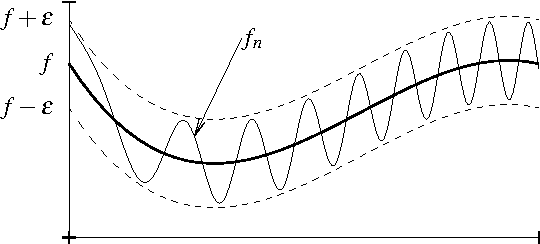
\includegraphics{figures/uniformconv}
\caption{In uniform convergence,
for $n \geq N$,
the functions $f_n$ are within a strip of $\pm\epsilon$ from $f$.%
\label{fig:uniformconv}}
\end{myfig}

\begin{exbox}
\begin{exercise} \label{exercise:limitnotcont}
Let $f_n(x)=x^n$ be functions on $[0,1]$.
\begin{exparts}
\item
Show that $\{ f_n \}$ converges pointwise to a discontinuous function.
\item
Prove that $\{ f_n \}$ converges
pointwise but not uniformly.
\end{exparts}
\end{exercise}

\begin{exercise}
Suppose $f_n \colon S \to \R$ are functions that converge uniformly
to $f \colon S \to \R$.  Suppose $A \subset S$.  Show that
the sequence of restrictions $\{ f_n|_A \}$ converges uniformly to $f|_A$.
\end{exercise}

\begin{exercise}
\begin{exparts}
\item
Suppose $\{ f_n \}$ and $\{ g_n \}$ defined on some set $A$ converge to
$f$ and $g$ respectively pointwise, and let $a,b \in \R$.
Show that $\{ a f_n+ b g_n \}$ converges
pointwise to $a f+ b g$.
\item
Show the same for uniform convergence.
\end{exparts}
\end{exercise}

\begin{exercise}
Find an example of a sequence of functions $\{ f_n \}$ and $\{ g_n \}$
that converge uniformly to some $f$ and $g$ on some set $A$, but such that
$\{ f_ng_n \}$ (the multiple) does not converge uniformly to $fg$ on $A$.
\end{exercise}

\begin{exercise}
Suppose there exists a sequence of functions $\{ g_n \}$ uniformly
converging to $0$ on $A$.  Now suppose we have a sequence of functions
$\{ f_n \}$ and a function $f$ on $A$ such that
\begin{equation*}
\abs{f_n(x) - f(x)} \leq g_n(x) 
\end{equation*}
for all $x \in A$.  Show that $\{ f_n \}$ converges uniformly to $f$ on $A$.
\end{exercise}

\begin{exercise}
Let $\{ f_n \}$, $\{ g_n \}$ and $\{ h_n \}$ be sequences of functions on
some set $S$.
Suppose $\{ f_n \}$ and $\{ h_n \}$ converge uniformly to some function
$f \colon S \to \R$ and suppose $f_n(x) \leq g_n(x) \leq h_n(x)$
for all $x \in S$.  Show that $\{ g_n \}$ converges uniformly to $f$.
\end{exercise}

\begin{exercise}
Prove that
if a sequence of functions $f_n \colon S \to \R$
converge uniformly to a bounded function $f \colon S \to \R$,
then there exists an $N$ such that for all $n \geq N$, the $f_n$
are bounded.
\end{exercise}
\end{exbox}

\begin{defn} \label{def:unifnorm}
For $f \colon S \to \R$, define
the \emph{\myindex{uniform norm}},
\glsadd{not:uniformnorm}%
\begin{equation*}
\snorm{f}_S
\overset{\text{def}}{=}
\sup \bigl\{ \sabs{f(x)} : x \in S \bigr\} .
\end{equation*}
\end{defn}

Note that if $f$ is not bounded, then $\snorm{f}_S = \infty$.  Therefore,
unless dealing with bounded functions, we treat the norm as an extended real,
so it is not what people would call a \myquote{norm} unless we restrict to bounded functions.

\begin{prop}
A sequence $f_n \colon S \to \R$ converges
uniformly to $f \colon S \to \R$ if and only if
\begin{equation*}
\lim_{n\to\infty} \snorm{f_n - f}_S = 0 .
\end{equation*}
\end{prop}

\begin{exbox}
\begin{exercise}
Prove the proposition.
\end{exercise}
\end{exbox}

We may say
\emph{$\{ f_n \}$ converges to $f$ in uniform norm}
\index{converges in uniform norm}%
\index{uniform norm convergence}%
instead of \emph{converges uniformly}.  The proposition
says that the two notions are the same thing.
It is generally easiest to think about uniform convergence of functions
using metric spaces.
A Cauchy sequence of functions in the uniform norm is said to be
\emph{\myindex{Cauchy in the uniform norm}} or
\emph{\myindex{uniformly Cauchy}}.

\begin{prop}
The set of bounded real-valued functions on $S$ is a complete metric space with
the metric $d(f,g) = \snorm{f-g}_S$.
In particular, if a sequence is uniformly Cauchy, then it is uniformly
convergent.
\end{prop}

\begin{exbox}
\begin{exercise}
Prove the proposition.  There are two things to prove.  First,
prove that the set is a metric space, that is, $d(f,g)$ is a metric.
Second, prove that it is complete.
\end{exercise}
\end{exbox}

\begin{remark}
It is perhaps surprising that on the set of functions $f \colon S \to
\R$ for an uncountable $S$, there is no metric that gives pointwise convergence.
You could even require $f$ to be bounded and/or continuous, and there is
still no metric.
A metric space $(X,d)$ is so-called \emph{\myindex{first countable}}, that
is, at each $x \in X$ there exists a sequence of neighbourhoods $U_j$ such
that any neighbourhood $U$ of $x$ contains one of the $U_j$s, a so-called
countable neighborhood basis.  In a metric space, $B(x,\nicefrac{1}{n})$
does the job.  But functions on an uncountable set $S$ with pointwise
convergence does not have a first countable topology.  We do not want to
wade too deep into into general topology to prove this fact.
\end{remark}

\subsection{Continuity of the limit}

If we have a sequence $\{ f_n \}$ of continuous functions,
is the limit continuous?  We have seen that for pointwise
convergence, this need not be the case, see \exerciseref{exercise:limitnotcont}.
If we, however, require the convergence to be uniform, the limits can
be interchanged.

\begin{thm} \label{thm:uniformlimitcont}
Let $S$ be a metric space.
Let $\{ f_n \}$ be 
a sequence of continuous functions $f_n \colon S \to \R$ converging
uniformly to  $f \colon S \to \R$.  Then $f$ is continuous.
\end{thm}

\begin{proof}
Let $x \in S$ be fixed.  Let $\{ x_n \}$ be a sequence in $S$
converging to $x$.
Let $\epsilon > 0$ be given.
As $\{ f_k \}$ converges uniformly to $f$, we find a $k \in \N$ such that
\begin{equation*}
\abs{f_k(y)-f(y)} < \nicefrac{\epsilon}{3}
\end{equation*}
for all $y \in S$.  As $f_k$ is continuous at $x$,
we find an $N \in \N$ such that for $m \geq N$
we have 
\begin{equation*}
\abs{f_k(x_m)-f_k(x)} < \nicefrac{\epsilon}{3} .
\end{equation*}
Thus for
$m \geq N$,
\begin{equation*}
\begin{split}
\abs{f(x_m)-f(x)}
& =
\abs{f(x_m)-f_k(x_m)+f_k(x_m)-f_k(x)+f_k(x)-f(x)}
\\
& \leq
\abs{f(x_m)-f_k(x_m)}+
\abs{f_k(x_m)-f_k(x)}+
\abs{f_k(x)-f(x)}
\\
& <
\nicefrac{\epsilon}{3} +
\nicefrac{\epsilon}{3} +
\nicefrac{\epsilon}{3} = \epsilon .
\end{split}
\end{equation*}
Therefore, $\{ f(x_m) \}$ converges to $f(x)$ and hence $f$ is continuous at
$x$.  As $x$ was arbitrary, $f$ is continuous everywhere.
\end{proof}

In the language of metric spaces,
as uniform limits of continuous functions are continuous,
the set of bounded continuous functions is a complete metric space.
The proof is left as an exercise.
More precisely,
let $C_b(S,\R)$ denote the set of bounded real-valued continuous functions on $S$.
We use the uniform norm as metric and $C_b(S,\R)$ is a metric space
for any $S$.  If $S$ is compact, then all continuous functions are bounded
and $C(S,\R)$ itself is a metric space.

\begin{cor} \label{cor:CSRcomplete}
Let $S$ be a metric space.  Then $C_b(S,\R)$ is a complete metric space.
If $S$ is compact, then $C(S,\R)$ is a complete metric space.
\end{cor}

\begin{exbox}
\begin{exercise}%[\neededexmark]
Prove \corref{cor:CSRcomplete}.
\end{exercise}
\end{exbox}

\begin{defn}
A sequence of functions $f_n \colon S \to \R$
\emph{\myindex{converges uniformly on compact subsets}}
\index{uniform convergence on compact subsets}
if for every compact $K \subset S$
the sequence $\{ f_n \}$ converges uniformly on $K$.
\end{defn}

\begin{cor} \label{cor:uniformkptlimitcont}
Let $U \subset \R^n$ be open.
If $f_n \colon U \to \R$ is a sequence of
continuous functions converging uniformly on compact subsets, then
the limit is continuous.
\end{cor}

\begin{exbox}
\begin{exercise}
Prove the corollary.
\end{exercise}
\end{exbox}

\subsection{Integral of the limit}

Again, if we simply require pointwise convergence, then the integral
of a limit of a sequence of functions need not be equal to the limit
of the integrals.

\begin{example}
Let $\chi_{T}$ be the characteristic function of a set $T$, that is, $\chi_T(x) =
1$ if $x \in T$ and $\chi_T(x) = 0$ otherwise.
The functions $n \chi_{(0,\nicefrac{1}{n})}$ all integrate (on the interval
$[0,1]$) to $1$.  Their
pointwise limit is $0$ (whose integral is $0$).
\end{example}

If we require the convergence to be uniform, the limits can
be interchanged.

\begin{thm} \label{integralinterchange:thm}
Let $\{ f_n \}$ be a sequence of Riemann integrable
functions
$f_n \colon [a,b] \to \R$
converging uniformly to $f \colon [a,b]
\to \R$.  Then $f$ is Riemann integrable and
\begin{equation*}
\int_a^b f(x) \, dx = \lim_{n\to\infty} \int_a^b f_n(x) \, dx .
\end{equation*}
\end{thm}

In the following, let 
$\overline{\int_a^b} f(x)\, dx$ and 
$\underline{\int_a^b} f(x)\, dx$ denote the upper and lower Darboux integral.
Briefly,
\begin{align*}
& \overline{\int_a^b} f(t) \,dt
\overset{\text{def}}{=}
\inf \left\{ \int_a^b s(t) \, dt : s
\text{ is a step function and } f(t) \leq s(t) \text{ for } t \in
[a,b] \right\} ,
\\
& \underline{\int_a^b} f(t) \,dt
\overset{\text{def}}{=}
\inf \left\{ \int_a^b s(t) \, dt : s
\text{ is a step function and } s(t) \leq f(t) \text{ for } t \in
[a,b] \right\} .
\end{align*}


The definition of the Riemann integral using Darboux sums and integrals is
beyond the scope of this book, but let us just mention that 
if the upper and lower Darboux integrals are equal, then a function is
Riemann integrable, and the common value is the integral.  Given this,
let us prove the theorem.

\begin{proof}
Let $\epsilon > 0$ be given.
As $f_n$ goes to $f$ uniformly, we find an $M \in \N$ such that
for all $n \geq M$ we have 
$\abs{f_n(x)-f(x)} < \frac{\epsilon}{2(b-a)}$ for all $x \in [a,b]$.
In particular, by reverse triangle inequality
$\abs{f(x)} < \frac{\epsilon}{2(b-a)} + \abs{f_n(x)}$ for all $x$,
hence $f$ is bounded
as $f_n$ is bounded.
Note that $f_n$ is integrable and compute
\begin{align*}
\overline{\int_a^b} & f(x) \, dx
-
\underline{\int_a^b} f(x) \, dx
\\
& =
\overline{\int_a^b} \bigl( f(x) - f_n(x) + f_n(x) \bigr) \, dx
-
\underline{\int_a^b} \bigl( f(x) - f_n(x) + f_n(x) \bigr) \, dx
\displaybreak[0]\\
& \leq
\overline{\int_a^b} \bigl( f(x) - f_n(x) \bigr) \, dx +  \overline{\int_a^b}
f_n(x) \, dx
-
\underline{\int_a^b} \bigl( f(x) - f_n(x) \bigr) \, dx -
\underline{\int_a^b} f_n(x) \, dx
\displaybreak[0]\\
& =
\overline{\int_a^b} \bigl( f(x) - f_n(x) \bigr)\, dx +  \int_a^b f_n(x) \, dx
-
\underline{\int_a^b} \bigl( f(x) - f_n(x) \bigr)\, dx -  \int_a^b f_n(x) \, dx
\displaybreak[0]\\
& =
\overline{\int_a^b} \bigl( f(x) - f_n(x) \bigr)\, dx
-
\underline{\int_a^b} \bigl( f(x) - f_n(x) \bigr)\, dx
\\
& \leq
\frac{\epsilon}{2(b-a)} (b-a) + 
\frac{\epsilon}{2(b-a)} (b-a) = \epsilon .
\end{align*}
The first inequality
is due to the upper integral being
only subadditive ($\overline{\int} (a+b) \leq \overline{\int}a +
\overline{\int} b$) and the lower integral being superadditive.
The final inequality follows from
the fact that for all $x \in [a,b]$ we have
$\frac{-\epsilon}{2(b-a)} < f(x)-f_n(x) < \frac{\epsilon}{2(b-a)}$.
As $\epsilon > 0$ was arbitrary, $f$ is Riemann integrable.

We compute $\int_a^b f(x)\,dx$.
For $n \geq M$ ($M$ is the same as above),
\begin{equation*}
\begin{split}
\abs{\int_a^b f(x)\,dx - \int_a^b f_n(x) \, dx} & = 
\abs{\int_a^b \bigl(f(x) - f_n(x)\bigr) \, dx}
\\
& \leq
\frac{\epsilon}{2(b-a)} (b-a) = \frac{\epsilon}{2} < \epsilon .
\end{split}
\end{equation*}
Therefore $\bigl\{ \int_a^b f_n(x) \,dx \bigr\}$ converges to $\int_a^b f(x) \,dx$.
\end{proof}

\begin{remark}
While we will not require the Lebesgue integral in this book, note that
for Lebesgue integral a much stronger convergence theorem holds.  In
particular, the dominated convergence theorem implies that if
$\{ f_n \}$ is a sequence of measurable functions on $[a,b]$,
converging pointwise to $f \colon [a,b] \to \R$, and such that
$\{ f_n \}$ is uniformly bounded (there is a single $B \in \R$ such that
$\snorm{f_n}_{[a,b]} \leq B$ for all $n$), then
\begin{equation*}
\int_a^b f(x) \, dx = \lim_{n\to\infty} \int_a^b f_n(x) \, dx .
\end{equation*}
Where of course all the integrals would have to be the Lebesgue integrals,
not the Riemann integrals.  The pointwise limit of Riemann integrable
functions need not even be Riemann integrable.
\end{remark}

\begin{exbox}
\begin{exercise}
Compute
$\displaystyle \lim_{n\to\infty} \int_1^2 e^{-nx^2} \,dx$.
\end{exercise}

\begin{exercise}
Find a sequence of Riemann integrable functions $f_n \colon [0,1] \to \R$ such
that $\{ f_n \}$ converges to zero pointwise, and such that
\begin{exparts}
\item
$\bigl\{ \int_0^1 f_n(x)\,dx \bigr\}_{n=1}^\infty$ increases without bound,
\item
$\bigl\{ \int_0^1 f_n(x)\,dx \bigr\}_{n=1}^\infty$ is the sequence $-1,1,-1,1,-1,1, \ldots$.
\end{exparts}
\end{exercise}
\end{exbox}

\subsection{Derivative of the limit}

While uniform convergence is enough to swap limits with integrals, it is not,
however, enough to swap limits with derivatives, unless you also have
uniform convergence of the derivatives themselves.

\begin{example}
The functions $f_n(x) = \frac{\sin(nx)}{n}$
converge uniformly to $0$.
See \figureref{fig:conv1nsinxn}.
The derivative of the limit is $0$.
But $f_n'(x) = \cos(nx)$,
which does not converge even pointwise,
for example, $f_n'(\pi) = {(-1)}^n$.
Furthermore, $f_n'(0) = 1$ for all $n$, which does converge, but not to $0$.
\begin{myfig}
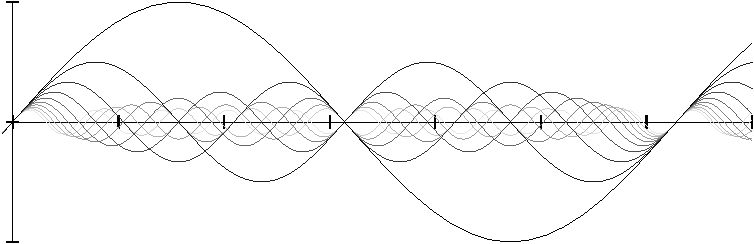
\includegraphics{figures/conv1nsinxn}
\caption{Graphs of $\frac{\sin(nx)}{n}$ for
$n=1,2,\ldots,10$, with higher $n$ in lighter gray.%
\label{fig:conv1nsinxn}}
\end{myfig}
\end{example}

The following theorem is true even if 
we do not assume continuity of the derivatives, but the proof is more
difficult.

\begin{thm} \label{thm:dersconverge}
Let $I$ be a bounded interval and let
$f_n \colon I \to \R$ be continuously differentiable functions.
Suppose $\{ f_n' \}$ converges uniformly to $g \colon I \to \R$,
and suppose $\{ f_n(c) \}_{n=1}^\infty$ is a
convergent sequence for some $c \in I$.  Then $\{ f_n \}$ converges uniformly to 
a continuously differentiable function $f \colon I \to \R$, and $f' = g$.
\end{thm}

\begin{proof}
Define $f(c) = \lim_{n\to \infty} f_n(c)$.
As $f_n'$ are continuous and hence Riemann integrable,
then
via the fundamental theorem of calculus, we find that for $x \in I$,
\begin{equation*}
f_n(x) = f_n(c) + \int_c^x f_n' (t)\, dt.
\end{equation*}
As $\{ f_n' \}$ converges uniformly on $I$, it converges uniformly
on $[c,x]$ (or $[x,c]$ if $x < c$).
Thus, the limit on the right-hand side exists.
Define $f$ at the remaining points by
\begin{equation*}
f(x) =
\lim_{n\to\infty} f_n(c) + \lim_{n\to\infty} \int_c^x f_n' (t)\, dt
=
f(c) + \int_c^x g(t)\,dt .
\end{equation*}
The function $g$ is continuous, being the uniform limit of continuous
functions.  Hence, $f$ is differentiable and $f'(x) = g(x)$ for all $x \in I$
by the fundamental theorem of calculus.

It remains to prove
uniform convergence.
Suppose $I$ has a lower bound $a$ and upper bound $b$.
Let $\epsilon > 0$ be given.  Take $M$
such that for $n \geq M$ we have
$\abs{f(c)-f_n(c)} < \nicefrac{\epsilon}{2}$
and
$\abs{g(x)-f_n'(x)} < \frac{\epsilon}{2(b-a)}$
for all $x \in I$.  Then,
\begin{equation*}
\begin{split}
\abs{f(x) - f_n(x)} & =
\abs{f(c) + \int_c^x g - f_n(c) - \int_c^x f_n'(t)\,dt}
\\
& \leq
\abs{f(c) - f_n(c)} + \abs{\int_c^x g(t)\,dt - \int_c^x f_n'(t)\,dt}
\\
& =
\abs{f(c) - f_n(c)} + \abs{\int_c^x \bigl(g(t) - f_n'(t)\bigr) \, dt}
\\
& <
\frac{\epsilon}{2}
+
\frac{\epsilon}{2(b-a)}
(b-a)
=\epsilon. \qedhere
\end{split}
\end{equation*}
\end{proof}

The proof goes through without boundedness of $I$, except for the
uniform convergence of $f_n$ to $f$.  For an example let $I = \R$ and
$f_n(x) = \nicefrac{x}{n}$.  Then $f_n'(x)=\nicefrac{1}{n}$, which
converges uniformly to $0$.  However, $\{f_n\}$ converges to $0$ only pointwise.

\begin{example}
In \exerciseref{exercise:C1ab}, you proved that
the set of once continuously differentiable functions on $[a,b]$, that is,
$C^1([a,b],\R)$, is a metric space with the so-called
$C^1$ metric (or $C^1$ norm)
\begin{equation*}
d(f,g) =
\snorm{f-g}_{C^1([a,b],\R)}
\overset{\text{def}}{=}
\snorm{f-g}_{[a,b]} + \snorm{f'-g'}_{[a,b]}.
\end{equation*}
The theorem says that $C^1([a,b],\R)$ is a complete metric space.
\end{example}

\begin{exbox}
\begin{exercise}
Find an explicit example of a sequence of
differentiable functions on $[-1,1]$ that converge uniformly to
a function $f$ such that $f$ is not differentiable.
Hint:
Perhaps $\sqrt{x^2+{(\nicefrac{1}{n})}^2}$?
\end{exercise}

\begin{exercise}
Let $f_n(x) = \frac{x^n}{n}$.  Show that $\{ f_n \}$ converges uniformly to
a differentiable function $f$ on $[0,1]$ (find $f$).  However, show that
$f'(1) \not= \lim\limits_{n\to\infty} f_n'(1)$.
\end{exercise}
\end{exbox}

%%%%%%%%%%%%%%%%%%%%%%%%%%%%%%%%%%%%%%%%%%%%%%%%%%%%%%%%%%%%%%%%%%%%%%%%%%%%%%

\section{Continuity, Fubini, derivatives under the integral}
\label{sec:contlimitsunderint}

\subsection{Continuity}

Let $f(x,y)$ be a function of two variables and define
\begin{equation*}
g(y) = \int_a^b f(x,y) \,dx .
\end{equation*}
Question is: Is $g$ is continuous?
We are really asking when do two limiting operations commute,
which is not always possible, so some extra hypothesis
is necessary.  A sufficient (but not
necessary) condition is that $f$ is continuous on a closed rectangle.

\begin{prop} \label{prop:integralcontcont}
If $f \colon [a,b] \times [c,d] \to \R$ is a continuous function,
then $g \colon [c,d] \to \R$ defined by
\begin{equation*}
g(y) = \int_a^b f(x,y) \,dx  \qquad \text{is continuous}.
\end{equation*}
\end{prop}

\begin{proof}
Fix $y \in [c,d]$, and let $\{ y_n \}$ be a sequence in $[c,d]$
converging to $y$.
Let $\epsilon > 0$ be given.
As $f$ is continuous on $[a,b] \times [c,d]$, which is compact, $f$
is uniformly continuous.  
In particular, there exists a $\delta > 0$ such that
whenever $\widetilde{y} \in [c,d]$ and
$\abs{\widetilde{y}-y} < \delta$ we have
$\abs{f(x,\widetilde{y})-f(x,y)} < \epsilon$ for all $x \in [a,b]$.
Let $h_n(x)= f(x,y_n)$ and $h(x) = f(x,y)$.
We have just shown that
$h_n \colon [a,b] \to \R$ converges uniformly 
to
$h \colon [a,b] \to \R$ as $n\to \infty$.
So we can take the limit underneath the integral:
\begin{equation*}
\lim_{n\to \infty}
g(y_n)
=
\lim_{n\to \infty}
\int_a^b 
f(x,y_n) \,dx 
= 
\int_a^b 
\lim_{n\to \infty}
f(x,y_n) \,dx 
= 
\int_a^b 
f(x,y) \,dx = g(y) . \qedhere
\end{equation*}
\end{proof}

In applications, if we are interested in continuity at $y_0$, we just
need to apply the proposition in $[a,b] \times [y_0-\epsilon,y_0+\epsilon]$
for some small $\epsilon > 0$.  For example, if $f$ is continuous in
$[a,b] \times \R$, then $g$ is continuous on $\R$.

\begin{exbox}
\begin{exercise} \label{exercise:integralcontcontextra}
Prove a stronger version of \propref{prop:integralcontcont}:
If $f \colon (a,b) \times (c,d) \to \R$ is a bounded continuous function,
then $g \colon (c,d) \to \R$ defined by
\begin{equation*}
g(y) = \int_a^b f(x,y) \,dx  \qquad \text{is continuous}.
\end{equation*}
Hint: First integrate over $[a+\nicefrac{1}{n},b-\nicefrac{1}{n}]$.
\end{exercise}
\end{exbox}

\subsection{Fubini's theorem}

Fubini's theorem says that under some mild conditions one can generally
swap the order of of integrals in an iterated integral.
We prove the following simple case of Fubini that is generally
enough for the purposes of this book.

\begin{thm}[Fubini]\index{Fubini's theorem}\label{thm:fubini}
Suppose $f \colon [a,b] \times [c,d] \to \R$ is continuous.  Then
\begin{equation*}
\int_c^d \int_a^b f(x,y) \, dx \, dy =
\int_a^b \int_c^d f(x,y) \, dy \, dx .
\end{equation*}
\end{thm}

One of the tricky bits about Fubini for the Riemann integral
is that the integrand of the outer integral, for example
$\int_a^b f(x,y) \, dx$ as a function of $y$, is not necessarily 
Riemann integrable even if $f(x,y)$ is Riemann integrable as a function of
two variables.  However, by the previous subsection, if $f$ is continuous,
then $\int_a^b f(x,y) \, dx$ is a continuous function of $y$ and hence
integrable.  So for continuous functions we sidestep the integrability
issues.\footnote{For more complicated scenarios, the reader is
encouraged to just learn the Lebesgue integral.}

\begin{proof}
As $[a,b] \times [c,d]$ is compact, $f$ is uniformly continuous.
So for
any $\epsilon > 0$, there is a $\delta > 0$ such that if
$\sabs{x-x'} < \delta$ and 
$\sabs{y-y'} < \delta$, then $\sabs{f(x,y) -f(x',y')} < \epsilon$.
Let
\begin{equation*}
g_n(x,y)
=
\begin{cases}
f(a,y) & \text{if } x=a ,
\\
f\left(a+\frac{k(b-a)}{n},y\right)
& \text{if } a+\frac{(k-1)(b-a)}{n} < x \leq a+\frac{k(b-a)}{n} , ~
k=1,\ldots,n.
\end{cases}
\end{equation*}
This is the \myquote{right-hand rule} step function with sub
interval length $\frac{b-a}{n}$:
Integrating $g_n$ with respect to $x$ is the right-hand rule for integrating $f$.
Let $n$ be large enough so that $\frac{b-a}{n} < \delta$.  Then,
via the uniform continuity estimate, we find that $\babs{f(x,y)-g_n(x,y)} < \epsilon$
for all $x$ and $y$. So
\begin{equation*}
\abs{
\int_a^b
f(x,y)
\, dx
-
\int_a^b
g_n(x,y)
\, dx
}
\leq
\int_a^b
\babs{
f(x,y)
-
g_n(x,y)
}
\leq (b-a)\epsilon .
\end{equation*}
So $\int_a^b g_n(x,y) \, dx$ converges uniformly as a function of $y$ to
$\int_a^b f(x,y) \, dx$.  Finally, the integral of $g_n$ is just the right
hand rule.  Putting it all together,
\begin{equation*}
\begin{split}
\int_c^d \int_a^b f(x,y) \, dx \, dy
& =
\int_c^d
\left(
\lim_{n \to \infty}
\int_a^b g_n(x,y) \, dx
\right) \, dy
\\
& =
\lim_{n \to \infty}
\int_c^d
\left(
\int_a^b g_n(x,y) \, dx
\right) \, dy
\\
& =
\lim_{n \to \infty}
\int_c^d
\left(
\sum_{k=1}^n
\frac{b-a}{n} f\left(a+\frac{k(b-a)}{n},y\right)
\right) \, dy
\\
& =
\lim_{n \to \infty}
\sum_{k=1}^n
\frac{b-a}{n} 
\int_c^d
f\left(a+\frac{k(b-a)}{n},y\right)
\, dy
\\
& =
\int_a^b
\int_c^d
f(x,y)
\, dy \, dx .
\end{split}
\end{equation*}
The final equation is simply the realization that  
$\int_c^d
f(x,y)
\, dy$ is a continuous function of $x$, hence integrable, and what we have
is just the right-hand rule for the integral of this function over $[a,b]$.
\end{proof}

\begin{exbox}
\begin{exercise}
Suppose $f(x,y) = 1$ if $x \in \Q$ and $y=\nicefrac{1}{2}$ and $0$ otherwise.
Using the Riemann integral, prove that one of
$\int_0^1 \int_0^1 f(x,y) \, dx \, dy$ and
$\int_0^1 \int_0^1 f(x,y) \, dy \, dx$ exists and the other does not (the
integrand is not a well-defined function).
\end{exercise}

\begin{exercise}
Compute
\begin{equation*}
\int_0^1 \int_0^1 \frac{x^2-y^2}{{(x^2+y^2)}^2} \, dx \, dy
\qquad \text{and} \qquad
\int_0^1 \int_0^1 \frac{x^2-y^2}{{(x^2+y^2)}^2} \, dy \, dx .
\end{equation*}
You will need to interpret the integrals as improper, that
is, the limit of $\int_\epsilon^1$ as $\epsilon \downarrow 0$.
\end{exercise}
\end{exbox}

\subsection{Differentiation under the integral}
\label{subsec:diffunderint}

Let $f(x,y)$ be a function of two variables and
\begin{equation*}
g(y) = \int_a^b f(x,y) \,dx .
\end{equation*}
If $f$ is continuous on $[a,b] \times [c,d]$, then
\propref{prop:integralcontcont}
says that $g$ is continuous on $[c,d]$.
Suppose $f$ is differentiable in $y$.
Can we \myquote{differentiate under the integral?}
Differentiation is a limit and we are again asking when do the
two limiting operations, integration and differentiation, commute.
The first
question we face is the integrability of
$\frac{\partial f}{\partial y}$, but the formula can fail even if
$\frac{\partial f}{\partial y}$ is integrable as a function of $x$ for every
fixed $y$.
We prove a simple, but perhaps the most useful, version of the theorem.

\begin{thm}[\myindex{Leibniz integral rule}]
\label{thm:Leibnizrule}
Suppose $f \colon [a,b] \times [c,d] \to \R$ is a continuous function,
such that $\frac{\partial f}{\partial y}$ exists for all $(x,y) \in [a,b]
\times [c,d]$ and is continuous.  Define
\begin{equation*}
g(y) = \int_a^b f(x,y) \,dx .
\end{equation*}
Then $g \colon [c,d] \to \R$ is continuously differentiable and
\begin{equation*}
g'(y) = \int_a^b \frac{\partial f}{\partial y}(x,y) \,dx .
\end{equation*}
\end{thm}

The hypotheses on $f$ and $\frac{\partial f}{\partial y}$ can be
weakened to a degree. See, e.g., \exerciseref{exercise:strongerleibniz}.
The proof below requires that
$\frac{\partial f}{\partial y}$ exists and is continuous
as a function of two variables, and the $x$ interval must be the entire
closed interval $[a,b]$.
The $y$ interval
$[c,d]$ can be replaced by a small (open or closed) interval if
needed, and in applications, we often make $[c,d]$ be a
small interval around the point where we need to differentiate.

\begin{proof}
Fix $y \in [c,d]$ and let $\epsilon > 0$ be given.
As $\frac{\partial f}{\partial y}$ is continuous on $[a,b] \times [c,d]$, it
is uniformly continuous.  In particular, there exists $\delta > 0$ such that
whenever $y_1 \in [c,d]$ with
$\sabs{y_1-y} < \delta$ and all $x \in [a,b]$ we have
\begin{equation*}
\abs{\frac{\partial f}{\partial y}(x,y_1)-\frac{\partial f}{\partial y}(x,y)} < \epsilon .
\end{equation*}

Suppose $h$ is such that $y+h \in [c,d]$ and $\sabs{h} < \delta$.
Fix $x$ for a moment
and apply the mean value theorem to find a $y_1$ between $y$ and $y+h$ such that
\begin{equation*}
\frac{f(x,y+h)-f(x,y)}{h}
=
\frac{\partial f}{\partial y}(x,y_1) .
\end{equation*}
As $\sabs{y_1-y} \leq \sabs{h} < \delta$,
\begin{equation*}
\abs{
\frac{f(x,y+h)-f(x,y)}{h}
-
\frac{\partial f}{\partial y}(x,y) 
}
=
\abs{
\frac{\partial f}{\partial y}(x,y_1) 
-
\frac{\partial f}{\partial y}(x,y) 
}
< \epsilon .
\end{equation*}
This argument worked for every $x \in [a,b]$.  Therefore, as a function of
$x$
\begin{equation*}
x \mapsto \frac{f(x,y+h)-f(x,y)}{h}
\quad
\text{converges uniformly to}
\quad
x \mapsto \frac{\partial f}{\partial y}(x,y)
\quad
\text{as } h \to 0 .
\end{equation*}
We defined uniform convergence for sequences although the idea is the
same.  You may replace $h$ with a sequence of nonzero 
numbers $\{ h_n \}$
converging to $0$ such that $y+h_n \in [c,d]$ and let $n \to \infty$.

Consider the difference quotient of $g$,
\begin{equation*}
\frac{g(y+h)-g(y)}{h}
=
\frac{\int_a^b f(x,y+h) \,dx -
\int_a^b f(x,y) \,dx }{h}
=
\int_a^b \frac{f(x,y+h)-f(x,y)}{h} \,dx .
\end{equation*}
Uniform convergence implies the limit can be taken underneath the integral.
So
\begin{equation*}
\lim_{h\to 0}
\frac{g(y+h)-g(y)}{h}
= 
\int_a^b 
\lim_{h\to 0}
\frac{f(x,y+h)-f(x,y)}{h} \,dx 
=
\int_a^b 
\frac{\partial f}{\partial y}(x,y) \,dx .
\end{equation*}
Then $g'$ is continuous on $[c,d]$ by
\propref{prop:integralcontcont}.
\end{proof}

\begin{example} \label{example:counterexamplediffunder}
Consider
\begin{equation*}
\int_0^{1} \frac{x-1}{\ln(x)} \,dx .
\end{equation*}
The integral exists as the function under the integral 
extends continuously to $[0,1]$, see \exerciseref{exercise:counterexamplediffunder}.
Trouble is finding it.  Introduce a parameter $y$
and define a function:
\begin{equation*}
g(y) = \int_0^{1} \frac{x^y-1}{\ln(x)} \,dx .
\end{equation*}
The function
$\frac{x^y-1}{\ln(x)}$
also extends to a continuous function of $x$ and $y$
for $(x,y) \in [0,1] \times [0,1]$ (also in the exercise).
See \figureref{fig:diffunderexample}.
\begin{myfig}
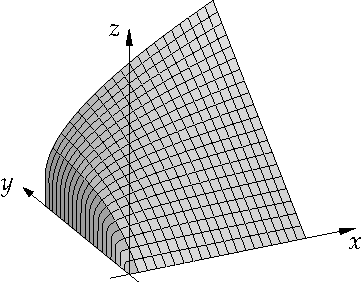
\includegraphics{figures/diffunderexample}
\caption{The graph $z= \frac{x^y-1}{\ln(x)}$ on $[0,1] \times [0,1]$.\label{fig:diffunderexample}}
\end{myfig}

Therefore,
$g$ is a continuous function of on $[0,1]$, and $g(0) = 0$.
For $0 < \epsilon < 1$, the $y$ derivative of the integrand, $x^y$,
is continuous on $[0,1] \times [\epsilon,1]$.  Therefore,
for $y >0$ we may differentiate under the integral sign
\begin{equation*}
g'(y) =
\int_0^{1} \frac{\ln(x) x^y}{\ln(x)} \,dx 
=
\int_0^{1} x^y \,dx =
\frac{1}{y+1} .
\end{equation*}
We know $g$ is continuous on $[0,1]$, $g(0)=0$, and
for $y \in (0,1)$, $g$ is differentiable and
$g'(y) = \frac{1}{y+1}$.  So $g(1) = \int_0^1 g'(y)\,dy = \ln(2)$.
In other words,
\begin{equation*}
\int_0^{1} \frac{x-1}{\ln(x)} \,dx  = \ln(2).
\end{equation*}
\end{example}

\begin{exbox}
\begin{exercise} \label{exercise:counterexamplediffunder}
Prove the two statements that were asserted in
\exampleref{example:counterexamplediffunder}:
\begin{exparts}
\item
Prove $\frac{x-1}{\ln(x)}$ extends to a continuous function of
$[0,1]$.  That is, there exists a continuous function on $[0,1]$
that equals $\frac{x-1}{\ln(x)}$ on $(0,1)$.
\item
Prove $\frac{x^y-1}{\ln(x)}$ extends to a continuous function
on $[0,1] \times [0,1]$.
\end{exparts}
\end{exercise}

\begin{exercise}
Suppose $h \colon \R \to \R$ is continuous and $g
\colon \R \to \R$ is continuously differentiable and compactly
supported ($g$ is zero outside a compact interval).  Define
\begin{equation*}
f(x) = \int_{-\infty}^\infty h(y)g(x-y) \, dy  .
\end{equation*}
Show that $f$ is differentiable.
\end{exercise}

\begin{exercise}
Suppose $f \colon \R \to \R$ is an infinitely differentiable function (all derivatives exist)
such that $f(0) = 0$.
\begin{exparts}
\item
Show that there exists an infinitely
differentiable function $g \colon \R \to \R$ such that $f(x) = x\,g(x)$.
\item
Show that
if $f'(0) \not= 0$, then $g(0) \not= 0$.
\end{exparts}
Hint: First write
$f(x) = \int_0^x f'(s) \,ds$ and then rewrite the integral to go
from $0$ to $1$.
\end{exercise}

\begin{exercise}%[\neededexmark]
\label{exercise:severalvariableLiebniz}
Let $U \subset \R^n$ be open and suppose
$f(x,y_1,y_2,\ldots,y_n)$ is a continuous
function defined on $[0,1] \times U \subset \R^{n+1}$.
Suppose
$\frac{\partial f}{\partial y_1},
\frac{\partial f}{\partial y_2},\ldots,
\frac{\partial f}{\partial y_n}$
exist and are continuous on $[0,1] \times U$.
Prove that $F \colon U \to \R$ defined by
\begin{equation*}
F(y_1,y_2,\ldots,y_n) =
\int_0^1
f(x,y_1,y_2,\ldots,y_n)
\, dx
\end{equation*}
is continuously differentiable (the partial derivatives exist and are
continuous).
\end{exercise}

\begin{exercise}
\pagebreak[2]
Work out the following counterexample:  Let
\begin{equation*}
f(x,y) =
\begin{cases}
\frac{xy^3}{{(x^2+y^2)}^2} & \text{if } x\not=0 \text{ or  } y\not= 0,\\
0 & \text{if } x=0 \text{ and } y=0.
\end{cases}
\end{equation*}
\begin{exparts}
\item
Prove that for each fixed $y$ the function $x \mapsto f(x,y)$ is
Riemann integrable on $[0,1]$ and
\begin{equation*}
g(y) = \int_0^1 f(x,y) \, dx = \frac{y}{2y^2+2} .
\end{equation*}
Therefore $g'(y)$ exists and we get the continuous function
\begin{equation*}
g'(y) = \frac{1-y^2}{2{(y^2+1)}^2} .
\end{equation*}
\item
Prove $\frac{\partial f}{\partial y}$ exists at all $x$ and $y$ and
compute it.
\item
Show that for all $y$
\begin{equation*}
\int_0^1 \frac{\partial f}{\partial y} (x,y) \, dx
\qquad
\text{exists, but}
\qquad
g'(0) \not= \int_0^1 \frac{\partial f}{\partial y} (x,0) \, dx .
\end{equation*}
\end{exparts}
\end{exercise}

\begin{exercise}
Work out the following counterexample:  Let
\begin{equation*}
f(x,y) =
\begin{cases}
x \,\sin \left(\frac{y}{x^2+y^2}\right) & \text{if } (x,y) \not= (0,0),\\
0 & \text{if } (x,y)=(0,0).
\end{cases}
\end{equation*}
\begin{exparts}
\item
Prove $f$ is continuous on all of $\R^2$.
Therefore the following function is well-defined for every $y \in \R$:
\begin{equation*}
g(y) = \int_0^1 f(x,y) \, dx .
\end{equation*}
\item
Prove $\frac{\partial f}{\partial y}$ exists for all $(x,y)$,
but is not continuous at $(0,0)$.
\item
Show that $\int_0^1 \frac{\partial f}{\partial y}(x,0) \, dx$ does not
exist even if we take improper integrals, that is,
that the limit
$\lim\limits_{h \downarrow 0} \int_h^1 \frac{\partial f}{\partial y}(x,0) \, dx$
does not exist.
\end{exparts}
Note: Feel free to use what you know about sine and cosine from calculus.
\pagebreak[2]
\end{exercise}

\begin{exercise} \label{exercise:strongerleibniz}
Strengthen the Leibniz integral rule in the following way.
Suppose $f \colon (a,b) \times (c,d) \to \R$ is a bounded continuous function,
such that $\frac{\partial f}{\partial y}$ exists for all $(x,y) \in (a,b)
\times (c,d)$ and is continuous and bounded.  Define
\begin{equation*}
g(y) = \int_a^b f(x,y) \,dx .
\end{equation*}
Then $g \colon (c,d) \to \R$ is continuously differentiable and
\begin{equation*}
g'(y) = \int_a^b \frac{\partial f}{\partial y}(x,y) \,dx .
\end{equation*}
Hint: See also \exerciseref{exercise:integralcontcontextra} and
\thmref{thm:dersconverge}.
\end{exercise}
\end{exbox}

%%%%%%%%%%%%%%%%%%%%%%%%%%%%%%%%%%%%%%%%%%%%%%%%%%%%%%%%%%%%%%%%%%%%%%%%%%%%%%

\section{The derivative in several real variables} \label{sec:derinsv}

\subsection{The derivative}

In the following, the norm $\snorm{\cdot}$ of a vector in $\R^n$
is the euclidean norm
\glsadd{not:euclidnorm}%
$\snorm{x} = \sqrt{x_1^2+\cdots+x_n^2}$.
When applied to a linear mapping (a matrix) it is the
\glsadd{not:operatornorm}%
\emph{\myindex{operator norm}}:
\begin{equation*}
\snorm{A} \overset{\text{def}}{=} \sup_{\snorm{x} = 1} \snorm{Ax} .
\end{equation*}
The following exercise collects some key facts about the operator norm
for the reader who has not seen this norm yet.

\begin{exbox}
\begin{exercise}
\begin{exparts} 
\item
Prove that if $A$ is a linear mapping between finite dimensional vector
spaces, then $\snorm{A} < \infty$.
\item
Prove that if $A$ is a linear mapping of vector spaces, then
$\snorm{Ax} \leq \snorm{A} \snorm{x}$.
\item
Find an explicit $2 \times 2$ matrix $A$ and a vector $x \in \R^2$
such that $\snorm{Ax} < \snorm{A} \snorm{x}$.
\item
If $A$ is a $1 \times n$ or $n \times 1$ matrix, then the operator norm
$\snorm{A}$ is the same as the euclidean norm of the entries of $A$.
\end{exparts} 
\end{exercise}
\end{exbox}

The derivative of $f \colon \R \to \R$ at $x \in \R$
exists if there is a number $a$ (the derivative of $f$ at $x$) such that
\begin{equation*}
\lim_{h \to 0} \abs{\frac{f(x+h)-f(x)}{h} - a} =
\lim_{h \to 0} \frac{\sabs{f(x+h)-f(x) - ah}}{\sabs{h}}
= 0.
\end{equation*}
Multiplying by $a$ is a linear map in one dimension:
$h \mapsto ah$.  So the derivative is a linear map.
Let us extend this idea to more variables.

\begin{defn}
Let $U \subset \R^n$ be open.  We say $f \colon U \to \R^m$
is \emph{(real) differentiable\index{real differentiable}}
at $x \in U$ if there exists
a linear $A \colon \R^n \to \R^m$ such that
\begin{equation*}
\lim_{\substack{h \to 0\\h\in \R^n}}
\frac{\snorm{f(x+h)-f(x) - Ah}}{\snorm{h}} = 0 .
\end{equation*}
We write $Df|_x = A$\glsadd{not:mvder} and
we say $A$ is the \emph{(real) derivative\index{real derivative}} of $f$ at $x$.
When $f$ is (real) differentiable at
every $x \in U$, we say that $f$ is \emph{(real) differentiable}.  See
\figureref{fig:svder}.
\end{defn}

\begin{myfig}
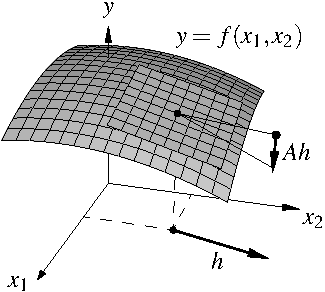
\includegraphics{figures/svder}
\caption{Illustration of a derivative for a function $f \colon \R^2 \to \R$.  The vector $h$ is shown
in the $x_1x_2$-plane based at $(x_1,x_2)$, and the vector
$Ah \in \R^1$ is shown along the $y$ direction.\label{fig:svder}}
\end{myfig}

Intuitively, $f$ is differentiable at $x$ if $f$ \myquote{infinitesimally close}
to a linear map near $x$.
We cheated a bit and said that $A$
is \emph{the} derivative, let us prove that we were justified.

\begin{prop}
Let $U \subset \R^n$ be open, $f \colon U \to \R^m$ a function,
$x \in U$, and 
$A,B \colon \R^n \to \R^m$ are linear such that
\begin{equation*}
\lim_{h \to 0}
\frac{\snorm{f(x+h)-f(x) - Ah}}{\snorm{h}} = 0
\qquad \text{and} \qquad
\lim_{h \to 0}
\frac{\snorm{f(x+h)-f(x) - Bh}}{\snorm{h}} = 0 .
\end{equation*}
Then $A=B$.
\end{prop}

\begin{proof}
Suppose $h \in \R^n$, $h \not= 0$.  Compute
\begin{equation*}
\begin{split}
\frac{\snorm{(A-B)h}}{\snorm{h}} & =
\frac{\snorm{f(x+h)-f(x) - Ah - (f(x+h)-f(x) - Bh)}}{\snorm{h}} \\
& \leq
\frac{\snorm{f(x+h)-f(x) - Ah}}{\snorm{h}} + \frac{\snorm{f(x+h)-f(x) -
Bh}}{\snorm{h}} .
\end{split}
\end{equation*}
So 
$\frac{\snorm{(A-B)h}}{\snorm{h}} = \bnorm{(A-B)\frac{h}{\snorm{h}}} \to 0$
as $h \to 0$.  Any point on the unit sphere can be written as $\frac{h}{\snorm{h}}$
for an arbitrarily small $h$, and a linear mapping vanishing on the unit sphere is
zero everywhere.
\end{proof}

\begin{example}
If $f(x) = Ax$ for a linear mapping $A$, then
$Df|_x = A$:
\begin{equation*}
\frac{\snorm{f(x+h)-f(x) - Ah}}{\snorm{h}}
=
\frac{\snorm{A(x+h)-Ax - Ah}}{\snorm{h}}
=
\frac{0}{\snorm{h}} = 0 .
\end{equation*}
\end{example}

\begin{example}
Let $f \colon \R^2 \to \R^2$ be defined by
\begin{equation*}
f(x,y) = \bigl(f_1(x,y),f_2(x,y)\bigr) = (1+x+2y+x^2,2x+3y+xy).
\end{equation*}
Let us show that $f$ is differentiable at the origin and 
compute the derivative,
directly using the definition.  If the
derivative exists, it can be
represented by a $2$-by-$2$ matrix
$\left[\begin{smallmatrix}a&b\\c&d\end{smallmatrix}\right]$.  Suppose $h =
(h_1,h_2)$.  We need the following expression to go to zero.
\begin{multline*}
\frac{\snorm{
f(h_1,h_2)-f(0,0)
-
(ah_1 +bh_2 , ch_1+dh_2)}
}{\snorm{(h_1,h_2)}}
=
\\
\frac{\sqrt{
{\bigl((1-a)h_1 + (2-b)h_2 + h_1^2\bigr)}^2
+
{\bigl((2-c)h_1 + (3-d)h_2 + h_1h_2\bigr)}^2}}{\sqrt{h_1^2+h_2^2}} .
\end{multline*}
If we choose $a=1$, $b=2$, $c=2$, $d=3$, the expression becomes
\begin{equation*}
\frac{\sqrt{
h_1^4 + h_1^2h_2^2}}{\sqrt{h_1^2+h_2^2}}
=
\sabs{h_1}
\frac{\sqrt{
h_1^2 + h_2^2}}{\sqrt{h_1^2+h_2^2}}
= \sabs{h_1} .
\end{equation*}
And this expression does indeed go to zero as $h \to 0$.  The
function $f$ is differentiable at the origin and 
the derivative $Df|_0$ is represented by the matrix
$\left[\begin{smallmatrix}1&2\\2&3\end{smallmatrix}\right]$.
\end{example}

\begin{prop}
Let $U \subset \R^n$ be open and $f \colon U \to \R^m$ be
differentiable at $p \in U$.  Then $f$ is continuous at $p$.
\end{prop}

\begin{proof}
Another way to write the differentiability of $f$ at $p$ is to first write
\begin{equation*}
r(h) = f(p+h)-f(p) - Df|_p h ,
\end{equation*}
and $\frac{\snorm{r(h)}}{\snorm{h}}$ must go to zero as $h \to 0$.
So
$r(h)$ itself must go to zero.  The mapping $h \mapsto Df|_p h$
is a linear mapping between finite dimensional spaces, it is
therefore continuous
and goes to zero as $h \to 0$.  So
$f(p+h)$ must go to $f(p)$ as $h \to 0$.
\end{proof}

The derivative is itself a linear operator on the space of differentiable
functions.

\begin{prop}
Suppose $U \subset \R^n$ is open,
$f \colon U \to \R^m$ and
$g \colon U \to \R^m$ are differentiable at $p$,
and $\alpha \in \R$.  Then the functions $f+g$ and $\alpha f$
are differentiable at $p$, and
\begin{equation*}
D(f+g)|_p = Df|_p + Dg|_p \qquad \text{and} \qquad D(\alpha f)|_p = \alpha
Df|_p .
\end{equation*}
\end{prop}

\begin{proof}
Let $h \in \R^n$, $h \not= 0$.  The proposition follows from the following
estimates:
\begin{multline*}
\frac{\norm{f(p+h)+g(p+h)-\bigl(f(p)+g(p)\bigr) - \bigl(Df|_p + Dg|_p\bigr)h}}{\snorm{h}}
\\
\leq
\frac{\norm{f(p+h)-f(p) - Df|_ph}}{\snorm{h}}
+
\frac{\norm{g(p+h)-g(p) - Dg|_ph}}{\snorm{h}} ,
\end{multline*}
and
\begin{equation*}
\frac{\norm{\alpha f(p+h) - \alpha f(p) - \alpha Df|_p h}}{\snorm{h}}
=
\sabs{\alpha} \frac{\norm{f(p+h))-f(p) - Df|_ph}}{\snorm{h}} .
\qedhere
\end{equation*}
\end{proof}

If $A \colon X \to Y$ and $B \colon Y \to Z$ are linear maps, then 
they are their own derivative.  The composition
$BA$, a linear map from $X$ to $Z$, is also its own derivative, and
so the derivative of the composition is the composition
of the derivatives.
As differentiable maps are \myquote{infinitesimally close}
to linear maps, they have the same property:

\begin{thm}[Chain rule]\index{chain rule!real derivative} \label{thm:realchain}
Let $U \subset \R^n$ be open and let $f \colon U \to \R^m$ be
differentiable at $p \in U$.  Let $V \subset \R^m$ be open,
$f(U) \subset V$ and let $g \colon V \to \R^\ell$ be differentiable
at $f(p)$.  Then
\begin{equation*}
F(x) = g\bigl(f(x)\bigr)
\end{equation*}
is differentiable at $p$ and
\begin{equation*}
DF|_p = Dg|_{f(p)} Df|_p .
\end{equation*}
\end{thm}

\begin{proof}
Let $A = Df|_p$ and $B = Dg|_{f(p)}$.  Take $h \in \R^n$
and write $q = f(p)$, $k = f(p+h)-f(p)$.  Let
\begin{equation*}
r(h) = f(p+h)-f(p) - A h .
\end{equation*}
Then $r(h) = k-Ah$ or $Ah = k-r(h)$, and $f(p+h) = q+k$.
\begin{equation*}
\begin{split}
\frac{\snorm{F(p+h)-F(p) - BAh}}{\snorm{h}}
& =
\frac{\snorm{g\bigl(f(p+h)\bigr)-g\bigl(f(p)\bigr) - BAh}}{\snorm{h}}
\\
& =
\frac{\snorm{g(q+k)-g(q) - B\bigl(k-r(h)\bigr)}}{\snorm{h}}
\\
& \leq
\frac
{\snorm{g(q+k)-g(q) - Bk}}
{\snorm{h}}
+
\snorm{B}
\frac
{\snorm{r(h)}}
{\snorm{h}}
\\
& =
\frac
{\snorm{g(q+k)-g(q) - Bk}}
{\snorm{k}}
\frac
{\snorm{f(p+h)-f(p)}}
{\snorm{h}}
+
\snorm{B}
\frac
{\snorm{r(h)}}
{\snorm{h}} .
\end{split}
\end{equation*}
First, $\snorm{B}$ is constant and $f$ is differentiable at $p$,
so
the term $\snorm{B}\frac{\snorm{r(h)}}{\snorm{h}}$ goes to $0$.
Next as $f$ is continuous at $p$, we have that as 
$h$ goes to $0$, then $k$ goes to $0$.  Therefore,
$\frac
{\snorm{g(q+k)-g(q) - Bk}}
{\snorm{k}}$ goes to $0$ because $g$ is differentiable at $q$.
Finally,
\begin{equation*}
\frac
{\snorm{f(p+h)-f(p)}}
{\snorm{h}}
\leq
\frac
{\snorm{f(p+h)-f(p)-Ah}}
{\snorm{h}}
+
\snorm{A} .
\end{equation*}
As $f$ is differentiable at $p$,
for small enough $h$, the quantity
$\frac{\snorm{f(p+h)-f(p)-Ah}}{\snorm{h}}$ is bounded.
Therefore, the term
$
\frac
{\snorm{f(p+h)-f(p)}}
{\snorm{h}}
$
stays bounded as $h$ goes to $0$.  Hence, 
$\frac{\snorm{F(p+h)-F(p) - BAh}}{\snorm{h}}$ goes to zero, and
$DF|_p = BA$, which is what was claimed.
\end{proof}

Let us prove a \myquote{mean value theorem} for vector-valued functions.
For a function $\varphi \colon [a,b] \to \R^n$, we think of the derivative
$D\varphi|_{t_0}$ as a vector, and so 
it is often just written as $\varphi'(t_0)$, it is not hard to check that
the entries of the matrix $D\varphi|_{t_0}$ are just the derivatives of the
components of $\varphi$, and $D\varphi|_{t_0} h = \varphi'(t_0) \cdot h$,
where $h$ is the dot product.  Then
$\snorm{\varphi'(t_0)}$
is the euclidean norm in $\R^n$.  And in fact, in this setting it is the same
as the operator norm.

\begin{lemma}
If $\varphi \colon [a,b] \to \R^n$ is differentiable on $(a,b)$ and
continuous on $[a,b]$, then there exists a $t_0 \in (a,b)$ such that
\begin{equation*}
\snorm{\varphi(b)-\varphi(a)} \leq (b-a) \snorm{\varphi'(t_0)} .
\end{equation*}
\end{lemma}

\begin{proof}
By the mean value theorem on the scalar-valued function
$t \mapsto \bigl(\varphi(b)-\varphi(a) \bigr) \cdot \varphi(t)$,
where the dot is the dot product, we obtain
that
there is a $t_0 \in (a,b)$ such that
\begin{equation*}
\begin{split}
\snorm{\varphi(b)-\varphi(a)}^2
& =
\bigl( \varphi(b)-\varphi(a) \bigr)
\cdot
\bigl( \varphi(b)-\varphi(a) \bigr)
\\
& =
\bigl(\varphi(b)-\varphi(a) \bigr) \cdot \varphi(b) - 
\bigl(\varphi(b)-\varphi(a) \bigr) \cdot \varphi(a)
\\
& = 
(b-a)
\bigl(\varphi(b)-\varphi(a) \bigr) \cdot \varphi'(t_0) .
\end{split}
\end{equation*}
By the Cauchy--Schwarz inequality
\begin{equation*}
\snorm{\varphi(b)-\varphi(a)}^2
=
(b-a)\bigl(\varphi(b)-\varphi(a) \bigr) \cdot \varphi'(t_0)
\leq
(b-a)
\snorm{\varphi(b)-\varphi(a)} \, \snorm{\varphi'(t_0)} . \qedhere
\end{equation*}
\end{proof}

Recall that a set $U$ is convex
if whenever $x,y \in U$, the line segment from
$x$ to $y$ lies in $U$.

\begin{prop} \label{mv:prop:convexlip}
Let $U \subset \R^n$ be a convex open set, $f \colon U \to \R^m$
a differentiable function, and $M$ be such that
\begin{equation*}
\snorm{Df|_x} \leq M
\qquad \text{for all } x \in U.
\end{equation*}
Then $f$ is Lipschitz with constant $M$, that is,
\begin{equation*}
\snorm{f(x)-f(y)} \leq M \snorm{x-y}
\qquad
\text{for all } x,y \in U.
\end{equation*}
\end{prop}

\begin{proof}
Fix $x,y \in U$.  By convexity,
$(1-t)x+ty \in U$ for all $t \in [0,1]$.
Next
\begin{equation*}
\frac{d}{dt} \Bigl[f\bigl((1-t)x+ty\bigr)\Bigr]
=
Df|_{((1-t)x+ty)} (y-x) .
\end{equation*}
By the mean value theorem above, for
some $t_0 \in (0,1)$,
\begin{equation*}
\begin{split}
\snorm{f(x)-f(y)} & \leq
\norm{\frac{d}{dt} \Big|_{t=t_0} \Bigl[ f\bigl((1-t)x+ty\bigr) \Bigr] }
\\
& \leq
\norm{Df|_{((1-t_0)x+t_0y)}} \, \snorm{y-x} \leq
M \snorm{y-x} . \qedhere
\end{split}
\end{equation*}
\end{proof}

Let us solve the differential equation $Df = 0$.

\begin{cor} \label{thm:svzerodersol}
If $U \subset \R^n$ is open and connected, $f \colon U \to \R^m$ is differentiable,
and $Df|_x = 0$ for all $x \in U$, then $f$ is constant.
\end{cor}

\begin{proof}
For any $x \in U$, there is an open ball $B(x,\delta) \subset U$.  The ball
$B(x,\delta)$ is convex.  Since
$\snorm{Df|_y} \leq 0$ for all $y \in B(x,\delta)$, then
$\snorm{f(x)-f(y)} \leq 0 \snorm{x-y} = 0$.
Thus $f^{-1}(c)$ is open for any $c \in \R^m$.  Suppose
$f^{-1}(c)$ is nonempty.  
The two sets
\begin{equation*}
U' = f^{-1}(c), \qquad U'' = f^{-1}\bigl(\R^m\setminus\{c\}\bigr)
\end{equation*}
are open and disjoint, and further $U = U' \cup U''$.  As $U'$ is nonempty
and $U$ is connected, then $U'' = \emptyset$.  So $f(x) = c$ for all $x \in U$.
\end{proof}

\begin{exbox}
\begin{exercise}
Using only the definition of the derivative, show that
the following $f \colon \R^2 \to \R^2$ are differentiable at the origin and
find their derivative.
\begin{exparts}
\item
$f(x,y) = (1+x+xy,x)$,
\item
$f(x,y) = \bigl(y-y^{10},x \bigr)$,
\item
$f(x,y) = \bigl( {(x+y+1)}^2 , {(x-y+2)}^2 \bigr)$.
\end{exparts}
\end{exercise}

\begin{exercise}
Define $f \colon \R^2 \to \R^2$ by $f(x,y) =
\bigl(x,y+\varphi(x)\bigr)$ for some differentiable function $\varphi$ of one
variable.  Show $f$ is differentiable and find $Df$.
\end{exercise}

\begin{exercise}
Suppose $f \colon \R^n \to \R$ and $h \colon \R^n \to \R$ are two 
differentiable functions such that $Df|_x = Dh|_x$ for all $x \in \R^n$.
Prove that
if $f(0) = h(0)$, then $f(x) = h(x)$ for all $x \in \R^n$.
\end{exercise}
\end{exbox}


\subsection{The derivative in terms of partial derivatives}

Partial derivatives are easier to compute with all the machinery of
calculus, and they provide a way to compute the derivative of a
function.

\begin{prop} \label{mv:prop:jacobianmatrix}
Let $U \subset \R^n$ be open and let $f \colon U \to \R^m$ be
differentiable at $p \in U$.  Then all the partial derivatives at $p$
exist and, in terms of the standard bases of $\R^n$ and $\R^m$,
$Df|_p$ is represented by the matrix
\begin{equation*}
\begin{bmatrix}
\frac{\partial f_1}{\partial x_1}\big|_p
&
\frac{\partial f_1}{\partial x_2}\big|_p
& \ldots &
\frac{\partial f_1}{\partial x_n}\big|_p
\\[6pt]
\frac{\partial f_2}{\partial x_1}\big|_p
&
\frac{\partial f_2}{\partial x_2}\big|_p
& \ldots &
\frac{\partial f_2}{\partial x_n}\big|_p
\\
\vdots & \vdots & \ddots & \vdots
\\
\frac{\partial f_m}{\partial x_1}\big|_p
&
\frac{\partial f_m}{\partial x_2}\big|_p
& \ldots &
\frac{\partial f_m}{\partial x_n}\big|_p
\end{bmatrix} .
\end{equation*}
\end{prop}

In other words,
\begin{equation*}
Df|_p \, e_j =
\sum_{k=1}^m
\frac{\partial f_k}{\partial x_j}\Big|_p \,e_k ,
\end{equation*}
where $e_j$ denote the vectors of the standard basis in the appropriate
space.  Recall that the standard basis element $e_j$ is the vector with all
zeros except a $1$ at the $j$\textsuperscript{th} entry.

\begin{proof}
Fix a $j$ and note that
\begin{equation*}
\begin{split}
\norm{\frac{f(p+h e_j)-f(p)}{h} - Df|_p \, e_j} & = 
\norm{\frac{f(p+h e_j)-f(p) - Df|_p \, h e_j}{h}} \\
& =
\frac{\snorm{f(p+h e_j)-f(p) - Df|_p \, h e_j}}{\snorm{h e_j}} .
\end{split}
\end{equation*}
As $h$ goes to $0$, the right-hand side goes to zero by
differentiability of $f$, and hence
\begin{equation*}
\lim_{h \to 0}
\frac{f(p+h e_j)-f(p)}{h} = Df|_p \, e_j  .
\end{equation*}
Let us represent $f$ by components
$f = (f_1,f_2,\ldots,f_m)$, since it is vector-valued.
Taking a limit in $\R^m$
is the same as taking the limit in each component separately.  
For any $k$,
\begin{equation*}
\frac{\partial f_k}{\partial x_j} \Big|_p
=
\lim_{h \to 0}
\frac{f_k(p+h e_j)-f_k(p)}{h}
\end{equation*}
exists and 
is equal to the $k$\textsuperscript{th} component of $Df|_p\, e_j$, and we are done.
\end{proof}

The converse of the proposition is not true.  Just because the partial
derivatives exist, does not mean that the function is differentiable.
However, when the partial derivatives are continuous, the
converse holds.


\begin{defn}
Let $U \subset \R^n$ be open.
We say $f \colon U \to \R^m$ is
\emph{\myindex{continuously differentiable}},
if all partial derivatives
$\frac{\partial f_j}{\partial x_k}$ exist and are continuous.\footnote{%
Alternatively, people define $f$ being continuously differentiable
if $Df|_x$ is a continuous function taking $x \in U$ to the space of linear
operators.  The propositions in this section say the two definitions are equivalent.}
\end{defn}

\begin{prop} \label{mv:prop:contdiffpartials}
Let $U \subset \R^n$ be open.
If $f \colon U \to \R^m$ is
continuously differentiable, then
$f$ is differentiable.
\end{prop}

\begin{proof}
Fix $x \in U$.  We do induction on dimension.  The case $n=1$ is left
as an exercise.
Suppose the conclusion is true for $\R^{n-1}$,
that is,
if we restrict to the first $n-1$ variables, the function is differentiable.
The first $n-1$
partial derivatives of $f$ restricted to the set where the last coordinate is
fixed are the same as those for $f$.
In the following, by a slight abuse of notation,
we think of $\R^{n-1}$ as a subset of $\R^n$, that is the set in $\R^n$ where $x_n = 0$.
In other words, we identify the vectors $(x_1,x_2,\ldots,x_{n-1})$ and
$(x_1,x_2,\ldots,x_{n-1},0)$.
Let
\begin{equation*}
A = 
\begin{bmatrix}
\frac{\partial f_1}{\partial x_1}\big|_x
& \ldots &
\frac{\partial f_1}{\partial x_n}\big|_x
\\
\vdots & \ddots & \vdots
\\
\frac{\partial f_m}{\partial x_1}\big|_x
& \ldots &
\frac{\partial f_m}{\partial x_n}\big|_x
\end{bmatrix} ,
\qquad
A' = 
\begin{bmatrix}
\frac{\partial f_1}{\partial x_1}\big|_x
& \ldots &
\frac{\partial f_1}{\partial x_{n-1}}\big|_x
\\
\vdots & \ddots & \vdots
\\
\frac{\partial f_m}{\partial x_1}\big|_x
& \ldots &
\frac{\partial f_m}{\partial x_{n-1}}\big|_x
\end{bmatrix} ,
\qquad
v = 
\begin{bmatrix}
\frac{\partial f_1}{\partial x_n}\big|_x
\\
\vdots
\\
\frac{\partial f_m}{\partial x_n}\big|_x
\end{bmatrix} .
\end{equation*}
Let $\epsilon > 0$ be given.  By the induction hypothesis, there
is a $\delta > 0$ such that
for any $k \in \R^{n-1}$ with $\snorm{k} < \delta$,
\begin{equation*}
\frac{\snorm{f(x+k) - f(x) - A' k}}{\snorm{k}} < \epsilon .
\end{equation*}
By continuity of the partial derivatives, suppose $\delta$ is small
enough so that
\begin{equation*}
\abs{\frac{\partial f_j}{\partial x_n}\Big|_{x+h}
      - \frac{\partial f_j}{\partial x_n}\Big|_{x}} < \epsilon ,
\end{equation*}
for all $j$ and all $h \in \R^n$ with $\snorm{h} < \delta$.

Suppose $h = k + t e_n$ is a vector in $\R^n$, where $k \in \R^{n-1}$, $t
\in \R$, such that
$\snorm{h} < \delta$.  Then $\snorm{k} \leq \snorm{h} < \delta$.
Note that $Ah = A' k + tv$.
\begin{equation*}
\begin{split}
\snorm{f(x+h) - f(x) - Ah}
& = \snorm{f(x+k + t e_n) - f(x+k) - tv + f(x+k) - f(x) - A' k}
\\
& \leq \snorm{f(x+k + t e_n) - f(x+k) -tv} + \snorm{f(x+k) - f(x) -
A' k}
\\
& \leq \snorm{f(x+k + t e_n) - f(x+k) -tv} + \epsilon \snorm{k} .
\end{split}
\end{equation*}
As all the partial derivatives exist, by the mean value theorem,
for each $j$ there is some $\theta_j \in [0,t]$ (or $[t,0]$ if $t < 0$), such that
\begin{equation*}
f_j(x+k + t e_n) - f_j(x+k) =
t \frac{\partial f_j}{\partial x_n}\Big|_{(x+k+\theta_j e_n)}.
\end{equation*}
Note that $\snorm{k+\theta_j e_n} \leq \snorm{h} < \delta$.
To finish,
\begin{equation*}
\begin{split}
\snorm{f(x+h) - f(x) - Ah}
& \leq \snorm{f(x+k + t e_n) - f(x+k) -tv} + \epsilon \snorm{k}
\\
& \leq \sqrt{\sum_{j=1}^m
{\left(t\frac{\partial f_j}{\partial x_n}\Big|_{(x+k+\theta_j e_n)} -
t \frac{\partial f_j}{\partial x_n}\Big|_{x}\right)}^2} + \epsilon \snorm{k}
\\
& \leq \sqrt{m}\, \epsilon \sabs{t} + \epsilon \snorm{k}
\\
& \leq (\sqrt{m}+1)\epsilon \snorm{h} . \qedhere
\end{split}
\end{equation*}
\end{proof}

\begin{exbox}
\begin{exercise}
Prove the base case
in \propref{mv:prop:contdiffpartials}:
If $n=1$ and 
\myquote{the partials exist and are continuous,} then the function is 
differentiable.  Note that $f$ is vector-valued.
\end{exercise}

\begin{exercise}
Define a function $f \colon \R^2 \to \R$ by
(see \figureref{fig:xyxsqysqvol2})
\begin{equation*}
f(x,y)
=
\begin{cases}
\frac{xy}{x^2+y^2} & \text{if } (x,y) \not= (0,0), \\
0 & \text{if } (x,y) = (0,0).
\end{cases}
\end{equation*}
\begin{exparts}
\item
Show that partial derivatives 
$\frac{\partial f}{\partial x}$ and
$\frac{\partial f}{\partial y}$ exist at all points (including the origin).
\item
Show that $f$ is not continuous at the origin (and hence not
differentiable).
\item
Show that the partial derivatives are not continuous.
\end{exparts}
\end{exercise}

\begin{exercise}
Define $f \colon \R^2 \to \R$ as
\begin{equation*}
f(x,y) =
\begin{cases}
(x^2+y^2)\sin\bigl({(x^2+y^2)}^{-1}\bigr) & \text{if } (x,y) \not= (0,0), \\
0 & \text{if } (x,y) = (0,0).
\end{cases}
\end{equation*}
Show that $f$ is differentiable at the origin, but that it is not 
continuously differentiable.
\end{exercise}
\end{exbox}

\begin{myfig}
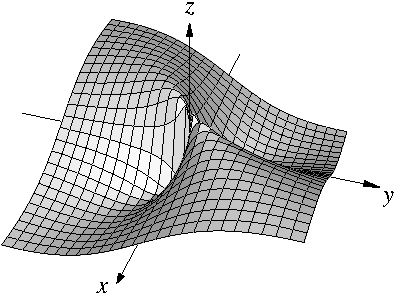
\includegraphics{figures/xyxsqysq}
\caption{Graph of $\frac{xy}{x^2+y^2}$.\label{fig:xyxsqysqvol2}}
\end{myfig}

\subsection{Fixed point theorem}

Before we prove the inverse function theorem we must take a detour to prove
a fixed point theorem for metric spaces.

\begin{defn}
Let $(X,d_X)$ and $(Y,d_Y)$ be metric spaces.
A mapping
$f \colon X \to Y$ is said to be a \emph{\myindex{contraction}}
(or a contractive map) if it is
a $k$-Lipschitz map for some $k < 1$, i.e., if there exists a $k < 1$ such that
\begin{equation*}
d_Y\bigl(f(p),f(q)\bigr) \leq k\, d_X(p,q)
\qquad \text{for all } p,q \in X.
\avoidbreak
\end{equation*}
If $f \colon X \to X$ is a map, $x \in X$ is called a
\emph{\myindex{fixed point}}
if $f(x)=x$.
\end{defn}

\begin{thm}%
[Contraction mapping principle\index{contraction mapping principle}
or \myindex{Banach fixed point theorem}\index{fixed point theorem}]
\label{thm:contr}
Let $(X,d)$ be a nonempty complete metric space and $f \colon X \to X$ a
contraction.
Then $f$ has a unique fixed point.
\end{thm}

\begin{proof}
Pick any $x_0 \in X$.
Define a sequence $\{ x_n \}$ by $x_{n+1} = f(x_n)$.
\begin{equation*}
d(x_{n+1},x_n) = d\bigl(f(x_n),f(x_{n-1})\bigr)
\leq k d(x_n,x_{n-1})
\leq \cdots
\leq k^n d(x_1,x_0) .
\end{equation*}
Suppose $m > n$, then
\begin{multline*}
d(x_m,x_n)
\leq \sum_{\ell=n}^{m-1} d(x_{\ell+1},x_\ell)
\leq \sum_{\ell=n}^{m-1} k^\ell d(x_1,x_0)
= k^n d(x_1,x_0) \sum_{\ell=0}^{m-n-1} k^\ell
\\
\leq k^n d(x_1,x_0) \sum_{\ell=0}^{\infty} k^\ell
= k^n d(x_1,x_0) \frac{1}{1-k} .
\end{multline*}
So the sequence is Cauchy.  Since $X$ is complete,
let $x = \lim\, x_n$.  We claim that $x$
is our unique fixed point.

Fixed point?  The function $f$ is a contraction,
so it is Lipschitz continuous:
\begin{equation*}
f(x) = f( \lim \, x_n) = \lim\, f(x_n) = \lim\, x_{n+1} = x .
\end{equation*}

Unique?  Let $x$ and $y$ both be fixed points.
\begin{equation*}
d(x,y) = d\bigl(f(x),f(y)\bigr) \leq k\, d(x,y) .
\end{equation*}
As $k < 1$ this means that $d(x,y) = 0$ and hence $x=y$.  The theorem is
proved.
\end{proof}

The proof is constructive.  Not only do we know 
a unique fixed point exists.  We also know how to find it.  Start with
any $x_0 \in X$ and iterate $f(x_0)$,
$f(f(x_0))$,
$f(f(f(x_0)))$, etc.

\begin{exbox}
\begin{exercise}
\begin{exparts}
\item
Find an example of a contraction $f \colon X \to X$
of a non-complete metric space $X$ with no
fixed point.
\item
Find a 1-Lipschitz map $f \colon X \to X$ of a complete metric space $X$ with no fixed point.
\end{exparts}
\end{exercise}

\begin{exercise}
Let $f(x) = x-\frac{x^2-2}{2x}$ (you may recognize Newton's method for
$\sqrt{2}$).
\begin{exparts}
\item
Prove $f\bigl([1,\infty)\bigr) \subset [1,\infty)$.
\item
Prove that $f \colon [1,\infty) \to [1,\infty)$ is a contraction.
\item
Apply the fixed point theorem to find an $x \geq 1$ such that
$f(x) = x$, and show that $x = \sqrt{2}$.
\end{exparts}
\end{exercise}
\end{exbox}

\subsection{Inverse function theorem}
\label{subsec:svinvfuncthm}

To prove the inverse function theorem, we use the contraction mapping
principle (\thmref{thm:contr}).
Intuitively, we again consider that if a function is continuously differentiable, then it
locally \myquote{behaves like} the derivative (a linear function).
The idea of the inverse function theorem is that if a function is
continuously differentiable and the derivative is invertible, the function is
(locally) invertible.

\begin{thm}[Inverse function theorem]\index{inverse function theorem}
\label{thm:inverse}
Suppose $U \subset \R^n$ is open, 
$f \colon U \to \R^n$ is continuously differentiable, $p \in U$, and $Df|_p$ is invertible
(that is, $\det Df|_p \not=0$).
Then there exist open sets $V, W \subset \R^n$ such that
$p \in V \subset U$, $f(V) = W$, the restriction $f|_V$ is injective (one-to-one),
and hence a $g \colon W \to V$ exists such that
$g(y) = (f|_V)^{-1}(y)$.
See \figureref{fig:inversefuncRn}.
Furthermore, $g$ is continuously differentiable
and 
\begin{equation*}
Dg|_y = {\bigl(Df|_x\bigr)}^{-1}, \qquad \text{for all } x \in V, y = f(x).
\end{equation*}
\end{thm}

\begin{myfig}
\subimport*{figures/}{inversefuncRn.pdf_t}
\caption{Setup of the inverse function theorem in $\R^n$.\label{fig:inversefuncRn}}
\end{myfig}

\begin{proof}
Write $A = Df|_p$.  As $Df$ is continuous, there exists an open ball
$V$ around $p$ such that
\begin{equation*}
\snorm{A-Df|_x} < \frac{1}{2\snorm{A^{-1}}}
\qquad \text{for all } x \in V.
\end{equation*}
The inequality implies that $Df|_x$ is invertible for all $x \in V$
(see exercise below).

Given $y \in \R^n$, define $\varphi_y \colon C \to \R^n$ by
\begin{equation*}
\varphi_y (x) = x + A^{-1}\bigl(y-f(x)\bigr) .
\end{equation*}
As $A^{-1}$ is one-to-one,
$\varphi_y(x) = x$ ($x$ is a fixed point) if only if
$y-f(x) = 0$, or in other words $f(x)=y$.  Using the chain rule we obtain
\begin{equation*}
D\varphi_y|_x = I - A^{-1} Df|_x = A^{-1} \bigl( A-Df|_x \bigr) .
\end{equation*}
So for $x \in V$,
\begin{equation*}
\snorm{D\varphi_y|_x} \leq \snorm{A^{-1}} \, \snorm{A-Df|_x} < \nicefrac{1}{2} .
\end{equation*}
As $V$ is a ball, it is convex.  Hence,
\begin{equation*}
\snorm{\varphi_y(x_1)-\varphi_y(x_2)} \leq \frac{1}{2} \snorm{x_1-x_2} 
\qquad
\text{for all } x_1,x_2 \in V.
\end{equation*}
In other words, $\varphi_y$ is a contraction defined on $V$, though we so far
do not know what is the range of $\varphi_y$.  We cannot yet
apply the fixed
point theorem, but we can say that $\varphi_y$ 
has at most one fixed point in $V$:
If $\varphi_y(x_1) = x_1$ and
$\varphi_y(x_2) = x_2$, then
$\snorm{x_1-x_2} = \snorm{\varphi_y(x_1)-\varphi_y(x_2)} \leq
\frac{1}{2} \snorm{x_1-x_2}$, so $x_1 = x_2$.
That is, there exists at most one $x \in V$
such that $f(x) = y$, and so $f|_V$ is one-to-one.

Let $W = f(V)$.  We need to show that $W$ is open.  Take a $y_0 \in W$.
There is a unique $x_0 \in V$ such that $f(x_0) = y_0$.
Let $r > 0$ be small enough such that the closed ball $C(x_0,r) \subset V$
(such $r > 0$ exists as $V$ is open).
Suppose $y$ is such that
\begin{equation*}
\snorm{y-y_0} <
\frac{r}{2\snorm{A^{-1}}} .
\end{equation*}
If we show that $y \in W$, then we have shown that $W$ is open.
If $x \in
C(x_0,r)$, then
\begin{equation*}
\begin{split}
\snorm{\varphi_y(x)-x_0}
& \leq
\snorm{\varphi_y(x)-\varphi_y(x_0)} +
\snorm{\varphi_y(x_0)-x_0} \\
& \leq
\frac{1}{2}\snorm{x-x_0} +
\snorm{A^{-1}(y-y_0)} \\
& \leq
\frac{1}{2}r +
\snorm{A^{-1}} \, \snorm{y-y_0} \\
& <
\frac{1}{2}r +
\snorm{A^{-1}}
\frac{r}{2\snorm{A^{-1}}} = r .
\end{split}
\end{equation*}
So $\varphi_y$ takes $C(x_0,r)$ into $B(x_0,r) \subset C(x_0,r)$.  It is a
contraction on $C(x_0,r)$ and $C(x_0,r)$ is complete (closed subset of $\R^n$
is complete).
Apply the contraction mapping principle to obtain a fixed point $x$,
i.e., $\varphi_y(x) = x$.  That is, $f(x) = y$, and $y \in
f\bigl(C(x_0,r)\bigr) \subset f(V) = W$.  Therefore, $W$ is open.

Next we need to show that $g$ is continuously differentiable and compute
its derivative.  First let us show that it is differentiable.
Consider $y \in W$ and $k \in \R^n$, $k\not= 0$, such that $y+k \in W$.
Because $f|_V$ is a one-to-one and onto mapping of $V$ onto $W$,
there are unique
$x \in V$ and $h \in \R^n$, where $h \not= 0$ and $x+h \in V$, such that
$f(x) = y$ and $f(x+h) = y+k$.
In other words, $g(y) = x$ and $g(y+k) = x+h$.  See
\figureref{fig:inversefuncRn2}.
\begin{myfig}
\subimport*{figures/}{inversefuncRn2.pdf_t}
\caption{Proving that $g$ is differentiable.\label{fig:inversefuncRn2}}
\end{myfig}

We can still
squeeze some information from the fact that $\varphi_y$ is a contraction.
\begin{equation*}
\varphi_y(x+h)-\varphi_y(x) = h + A^{-1} \bigl( f(x)-f(x+h) \bigr) = h - A^{-1} k .
\end{equation*}
So
\begin{equation*}
\snorm{h-A^{-1}k} = \snorm{\varphi_y(x+h)-\varphi_y(x)} \leq
\frac{1}{2}\snorm{x+h-x} = \frac{\snorm{h}}{2}.
\end{equation*}
By the inverse triangle inequality, $\snorm{h} - \snorm{A^{-1}k} \leq
\frac{1}{2}\snorm{h}$.
Hence,
\begin{equation*}
\snorm{h} \leq 2 \snorm{A^{-1}k} \leq 2 \snorm{A^{-1}} \, \snorm{k}.
\end{equation*}
In particular, as $k$ goes to $0$, so does $h$.

As $x \in V$, then $Df|_x$ is invertible.
Let $B = \bigl(Df|_x\bigr)^{-1}$, which is what we think the derivative of
$g$ at $y$ is.  Then
\begin{equation*}
\begin{split}
\frac{\snorm{g(y+k)-g(y)-Bk}}{\snorm{k}}
& =
\frac{\snorm{h-Bk}}{\snorm{k}}
\\
& =
\frac{\snorm{h-B\bigl(f(x+h)-f(x)\bigr)}}{\snorm{k}}
\\
& =
\frac{\snorm{B\bigl(f(x+h)-f(x)-Df|_x h\bigr)}}{\snorm{k}}
\\
& \leq
\snorm{B}
\frac{\snorm{h}}{\snorm{k}}\,
\frac{\snorm{f(x+h)-f(x)-Df|_x h}}{\snorm{h}}
\\
& \leq
2\snorm{B} \, \snorm{A^{-1}}
\frac{\snorm{f(x+h)-f(x)-Df|_x h}}{\snorm{h}} .
\end{split}
\end{equation*}
As $k$ goes to $0$, so does $h$, and, as $f$ is differentiable, so does the right-hand side.
So $g$ is differentiable with , and $B$
is precisely what we claimed $Dg|_y$ to be.

Let us show $g$ is continuously
differentiable.
The function $g \colon W \to V$ is continuous (it is differentiable),
$Df$ is a continuous function from $V$
to the space of $n \times n$ matrices (each entry is continuous),
and the inverse of a matrix $M$ is $M^{-1} = \frac{1}{\det M} \operatorname{adj} M$,
so $M \mapsto M^{-1}$ is continuous outside the set where $\det M = 0$.
As
$Dg|_y = {\bigl( Df|_{g(y)}\bigr)}^{-1}$ is the composition
of these three
continuous functions, it is continuous.
\end{proof}

\begin{example}
Just because $Df|_x$ is invertible everywhere does not
mean that $f$ is
one-to-one globally.  Consider
the map $f \colon \R^2 \setminus \{ 0 \} \to \R^2 \setminus \{
0 \}$ defined
by $f(x,y) = (x^2-y^2,2xy)$,  that is, the mapping $z \mapsto z^2$ in the
complex plane.  It is not hard to check that
the derivative is invertible on $\R^2 \setminus \{ 0 \}$.
On the other hand, the mapping is 2-to-1 globally (except at the origin).
For every $(a,b) \not= (0,0)$, there are exactly two
solutions to $x^2-y^2=a$ and $2xy=b$.
\end{example}

The invertibility of the derivative is not a necessary
condition, just sufficient, for having a continuous inverse and being an open
mapping.  For example, the function $f(x) = x^3$ is an open mapping from $\R$
to $\R$ and is globally one-to-one with a continuous inverse, although the
inverse is not differentiable at $x=0$.

\begin{remark}
As a side note, there is a related famous, and as yet unsolved problem,
called the \emph{\myindex{Jacobian conjecture}}.  If $F \colon \R^n \to \R^n$
(or more famously $F \colon \C^n \to \C^n$)
is polynomial (each component is a polynomial) and $\det DF$ is a nonzero
constant, does $F$ have a polynomial inverse?
The inverse function theorem gives a local $C^1$ inverse, but can one always
find a global polynomial inverse is the question.
\end{remark}

\begin{exbox}
\begin{exercise}
\begin{exparts}
\item
Suppose $A$ is a linear operator on $\R^n$ such that
$\snorm{I-A} < 1$ ($I$ is the identity). Prove that $A$ is invertible.
\item
For two linear operators $A$ and $B$ on $\R^n$ where $A$ is invertible,
prove that $\snorm{A-B} < \frac{1}{\snorm{A^{-1}}}$ implies that $B$ is
invertible.
\end{exparts}
\end{exercise}

\begin{exercise}
Define $f \colon \R^2 \to \R^2$ by $f(x,y) =
\bigl(x,y+h(x)\bigr)$ for some continuously differentiable function $h$ of one
variable.
\begin{exparts}
\item
Show that $f$ is one-to-one and onto.
\item
Compute $Df$.
\item
Show that $Df$ is invertible at all points, and compute
its inverse.
\end{exparts}
\end{exercise}

\begin{exercise}
Define $f \colon \R^2 \to \R^2$
\begin{equation*}
f(x,y) =
\begin{cases}
\bigl(x^2 \sin (\nicefrac{1}{x}) + \nicefrac{x}{2} , y \bigr) &
\text{if } x \not= 0, \\
(0,y) &
\text{if } x=0.
\end{cases}
\end{equation*}
\begin{exparts}
\item
Show that $f$ is differentiable everywhere.
\item
Show that $Df|_{(0,0)}$ is invertible.
\item
Show that $f$ is not one-to-one in every neighborhood of the origin (it is
not locally invertible, that is, the inverse function theorem does not work).
\item
Show that $f$ is not continuously differentiable.
\end{exparts}
\end{exercise}

\begin{exercise}[Polar coordinates]%[\neededexmark, Polar coordinates]
\label{mv:exercise:polarcoordinates}
\index{polar coordinates}
Define a mapping $F(r,\theta) = \bigl(r \cos(\theta), r \sin(\theta) \bigr)$.
\begin{exparts}
\item
Show that $F$ is continuously differentiable (for all $(r,\theta) \in
\R^2$).
\item
Compute $DF|_{(0,\theta)}$ for all $\theta$.
\item
Show that if $r \not= 0$, then $DF|_{(r,\theta)}$ is invertible, and so an
inverse of $F$ exists locally as long as $r \not= 0$.
\item
Show that $F \colon \R^2 \to \R^2$ is onto, and for each point $(x,y) \in
\R^2$, the set $F^{-1}(x,y)$ is infinite.
\item
Show that $F|_{(0,\infty) \times [0,2\pi)}$ is one-to-one and onto
$\R^2 \setminus \bigl\{ (0,0) \bigr\}$.
\end{exparts}
\end{exercise}
\end{exbox}

%%%%%%%%%%%%%%%%%%%%%%%%%%%%%%%%%%%%%%%%%%%%%%%%%%%%%%%%%%%%%%%%%%%%%%%%%%%%%%
%%%%%%%%%%%%%%%%%%%%%%%%%%%%%%%%%%%%%%%%%%%%%%%%%%%%%%%%%%%%%%%%%%%%%%%%%%%%%%
%%%%%%%%%%%%%%%%%%%%%%%%%%%%%%%%%%%%%%%%%%%%%%%%%%%%%%%%%%%%%%%%%%%%%%%%%%%%%%

\chapter{Basic Notation and Terminology} \label{ap:basicnotation}

%%%%%%%%%%%%%%%%%%%%%%%%%%%%%%%%%%%%%%%%%%%%%%%%%%%%%%%%%%%%%%%%%%%%%%%%%%%%%%

Let us quickly review some basic notation used.
We use $\C$, $\R$ for complex and real numbers ($i$ for imaginary unit),
$\N = \{ 1,2,3, \ldots \}$ for the natural numbers,
$\Z$ for all integers, and $\Q$ for rational real numbers.

\glsadd{not:setminus}%
We denote the set subtraction by 
$Y \setminus X$ (all elements of
$Y$ that are not in $X$).
\glsadd{not:complement}%
We write the complement of a set as $X^c$, in which case
the ambient set should be clear.
\glsadd{not:closure}%
The topological closure of a set $X$ is denoted by $\widebar{X}$ and its
boundary by
\glsadd{not:boundary}%
$\partial X$.  By $\partial X$ we may also mean the path that gives the
topological boundary traversed counterclockwise.
We write the interior of $X$ as
\glsadd{not:interior}%
$X^\circ$.

\glsadd{not:function}%
The notation $f \colon X \to Y$ is a function with domain $X$ and
codomain $Y$.  By $f(S)$ we mean the direct image of $S$ by $f$.
By $f^{-1}$ we mean the inverse image of sets and
single points, and if $f$ is bijective (one-to-one and onto),
we use it for the inverse mapping.
To define a function without necessarily giving it a name, we use
\glsadd{not:mapsto}%
\begin{equation*}
x \mapsto F(x) ,
\end{equation*}
where $F(x)$ would generally be some formula giving the output.
The notation
\glsadd{not:restriction}%
$f|_S$
means the restriction of $f$ to $S$:
a function
$f|_S \colon S \to Y$ such that $f|_S(x) = f(x)$ for all $x \in S$.
For derivatives, vertical bar means evaluation,
$\frac{\partial f}{\partial x}\big|_p$ means 
$\frac{\partial f}{\partial x}$ evaluated at $p$.
To say that two functions $f$ and $g$ are identically equal,
that is that $f(x) = g(x)$ for all $x$ in the domain,
we write
\glsadd{not:identeq}%
\begin{equation*}
f \equiv g .
\end{equation*}
The notation
\glsadd{not:composition}%
$f \circ g$
denotes the composition defined by $x \mapsto f\bigl(g(x)\bigr)$.

For one-sided limits we use
\glsadd{not:limupfunc}%
\glsadd{not:limdownfunc}%
\begin{equation*}
\lim_{t \uparrow a} f(t) \quad \Bigl( = \lim_{\substack{t \to a\\t < a}} f(t)
\Bigr)
\qquad \text{and} \qquad
\lim_{t \downarrow a} f(t) \quad \Bigl( = \lim_{\substack{t \to a\\t > a}} f(t)
\Bigr) ,
\end{equation*}
as these seemed the clearer option in some of the situations in this book.
We may write $\{ x_n \}$ for a sequence $\{x_n\}_{n=1}^\infty$ and similarly
$\lim x_n$ instead of $\lim_{n\to \infty} x_n$ when it is clear that $n$ is
the index of the sequence.

To define $X$ to be $Y$ rather than just show equality, we write
\glsadd{not:definition}%
\begin{equation*}
X
\overset{\text{def}}{=}
Y .
\end{equation*}

%%%%%%%%%%%%%%%%%%%%%%%%%%%%%%%%%%%%%%%%%%%%%%%%%%%%%%%%%%%%%%%%%%%%%%%%%%%%%%
%%%%%%%%%%%%%%%%%%%%%%%%%%%%%%%%%%%%%%%%%%%%%%%%%%%%%%%%%%%%%%%%%%%%%%%%%%%%%%
%%%%%%%%%%%%%%%%%%%%%%%%%%%%%%%%%%%%%%%%%%%%%%%%%%%%%%%%%%%%%%%%%%%%%%%%%%%%%%

%FIXME: else I don't get links, weird
%\def\MR#1{\relax\ifhmode\unskip\spacefactor3000 \space\fi%
  %\href{http://www.ams.org/mathscinet-getitem?mr=#1}{MR#1}}
\def\myDOI#1{\href{http://dx.doi.org/#1}{#1}}



%FIXME
%\cleardoublepage  
\clearpage
\phantomsection
\addcontentsline{toc}{chapter}{Further Reading}
\markboth{FURTHER READING}{FURTHER READING}
\begin{bibchapter}[Further Reading] \label{ch:furtherreading}

%Here we list useful books for extra reading.

\begin{biblist}[\normalsize]

\bib{Boas}{book}{
   author={Boas, Ralph P.},
   title={Invitation to complex analysis},
   series={MAA Textbooks},
   edition={2},
   note={Revised by Harold P. Boas},
   publisher={Mathematical Association of America, Washington, DC},
   date={2010},
   pages={xiv+327},
   isbn={978-0-88385-764-9},
   review={\MR{2674618}},
}

\bib{Conway1}{book}{
   author={Conway, John B.},
   title={Functions of one complex variable},
   series={Graduate Texts in Mathematics},
   volume={11},
   edition={2},
   publisher={Springer-Verlag, New York-Berlin},
   date={1978},
   pages={xiii+317},
   isbn={0-387-90328-3},
   review={\MR{503901}},
}

\bib{Conway2}{book}{
   author={Conway, John B.},
   title={Functions of one complex variable. II},
   series={Graduate Texts in Mathematics},
   volume={159},
   publisher={Springer-Verlag, New York},
   date={1995},
   pages={xvi+394},
   isbn={0-387-94460-5},
   review={\MR{1344449}},
   doi={10.1007/978-1-4612-0817-4},
}

\bib{ra:book}{misc}{
   author={Lebl, Ji\v{r}\'i},
   title={Basic analysis I: Introduction to real analysis, Volume I},
   note={\url{https://www.jirka.org/ra/}}
}

\bib{ra:book2}{misc}{
   author={Lebl, Ji\v{r}\'i},
   title={Basic analysis II: Introduction to real analysis, Volume II},
   note={\url{https://www.jirka.org/ra/}}
}

\bib{scv:book}{misc}{
   author={Lebl, Ji\v{r}\'i},
   title={Tasty bits of several complex variables},
   note={\url{https://www.jirka.org/scv/}}
}

\bib{Rudin:principles}{book}{
   author={Rudin, Walter},
   title={Principles of mathematical analysis},
   edition={3},
   note={International Series in Pure and Applied Mathematics},
   publisher={McGraw-Hill Book Co., New York-Auckland-D\"usseldorf},
   date={1976},
   pages={x+342},
   review={\MR{0385023}},
}

\bib{Rudin}{book}{
   author={Rudin, Walter},
   title={Real and complex analysis},
   edition={3},
   publisher={McGraw-Hill Book Co., New York},
   date={1987},
   pages={xiv+416},
   isbn={0-07-054234-1},
   review={\MR{924157}},
}

\bib{Ullrich}{book}{
   author={Ullrich, David C.},
   title={Complex made simple},
   series={Graduate Studies in Mathematics},
   volume={97},
   publisher={American Mathematical Society, Providence, RI},
   date={2008},
   pages={xii+489},
   isbn={978-0-8218-4479-3},
   review={\MR{2450873}},
   doi={10.1090/gsm/097},
}

\end{biblist}
\end{bibchapter}

%%%%%%%%%%%%%%%%%%%%%%%%%%%%%%%%%%%%%%%%%%%%%%%%%%%%%%%%%%%%%%%%%%%%%%%%%%%%%%
%%%%%%%%%%%%%%%%%%%%%%%%%%%%%%%%%%%%%%%%%%%%%%%%%%%%%%%%%%%%%%%%%%%%%%%%%%%%%%
%%%%%%%%%%%%%%%%%%%%%%%%%%%%%%%%%%%%%%%%%%%%%%%%%%%%%%%%%%%%%%%%%%%%%%%%%%%%%%

%\cleardoublepage  
\clearpage  
\phantomsection
\addcontentsline{toc}{chapter}{\indexname}  
\microtypesetup{protrusion=false}
\printindex
\microtypesetup{protrusion=true}

%%%%%%%%%%%%%%%%%%%%%%%%%%%%%%%%%%%%%%%%%%%%%%%%%%%%%%%%%%%%%%%%%%%%%%%%%%%%%%
%%%%%%%%%%%%%%%%%%%%%%%%%%%%%%%%%%%%%%%%%%%%%%%%%%%%%%%%%%%%%%%%%%%%%%%%%%%%%%
%%%%%%%%%%%%%%%%%%%%%%%%%%%%%%%%%%%%%%%%%%%%%%%%%%%%%%%%%%%%%%%%%%%%%%%%%%%%%%

%
% automake on glossaries doesn't work if the index is before the glossary.
% That's why the List of Notation is last, no other reason.  Problem is
% that printindex does a clearpage which screws up the delayed write18
% that glossaries sets up
%

\begingroup
\renewcommand{\pagelistname}{Page}
\setglossarystyle{long3colheader}
% correctly set up with cellspace
\renewenvironment{theglossary}%
  {\setlength\cellspacetoplimit{4pt}
   \setlength\cellspacebottomlimit{4pt}
   \setlength\LTleft{0pt}
   \setlength\LTright{0pt}
   \markboth{LIST OF NOTATION}{LIST OF NOTATION}
   \begin{longtable}{Sl @{\extracolsep{\fill}} Sl @{\extracolsep{\fill}} Sl}}%
  {\end{longtable}}%
\cleardoublepage
\microtypesetup{protrusion=false}
\printglossary[type=notation] 
\microtypesetup{protrusion=true}
\endgroup

\end{document}
